\documentclass[a4paper, hidelinks]{book}
\usepackage[utf8]{inputenc}
\usepackage[T1]{fontenc}
\usepackage{polski}
\usepackage[margin = 2.5cm]{geometry}
\usepackage{anyfontsize}
\usepackage{amsmath}
\usepackage{amssymb}
\usepackage{amsfonts}
\usepackage{amsthm}
\usepackage{dsfont}
\usepackage[shortlabels]{enumitem}
\usepackage{mathdots}
\usepackage{array}
\usepackage{enumitem}
\usepackage{hyperref} % referencje do miejsc w pdfie
\usepackage{url}
\usepackage{xfrac} % ukośne ułamki
\usepackage{cancel} % skracanie
\usepackage{environ} % zaawansowane środowiska
\usepackage{minted} % formatowanie kodu
\usepackage{tabularx} % lepsze tabelki
\usepackage{wrapfig} % do ustawiania pozycji obrazków
\usepackage{multicol} % wiele kolumn
\usepackage{bussproofs} % logika

% --- Podstawowe matematyczne symbole
\newcommand{\wtw}{\quad \Leftrightarrow \quad}  % wtedy i tylko wtedy
\newcommand{\bigexists}{\mbox{\Large $\mathsurround0pt\exists$}\hspace{0.2em}} 
\newcommand{\bigforall}{\mbox{\Large $\mathsurround0pt\forall$}\hspace{0.1em}}
\newcommand{\lr}[1]{\left\langle #1 \right\rangle}

% --- Oznaczenia zbiorów i grup
\newcommand{\RR}{\mathbb{R}}
\newcommand{\ZZ}{\mathbb{Z}}
\newcommand{\NN}{\mathbb{N}}
\newcommand{\CC}{\mathbb{C}}
\newcommand{\KK}{\mathbb{K}}
\newcommand{\QQ}{\mathbb{Q}}
\newcommand{\GG}{\mathbb{G}}

% --- Tekst w math mode
\newcommand{\dm}[1]{\displaystyle{#1}}  % skrót do displaystyle
\newcommand{\textq}[1]{\quad \text{#1} \quad}
\newcommand{\textqq}[1]{\qquad \text{#1} \qquad}

% --- Analiza matematyczna
\newcommand{\Dom}{\operatorname{Dom}}
\newcommand{\sgn}{\operatorname{sgn}}
\newcommand{\floor}[1]{\left\lfloor #1 \right\rfloor}
\newcommand{\ceil}[1]{\left\lceil #1 \right\rceil}
\newcommand{\inj}{\xrightarrow[]{1-1}}
\newcommand{\surj}{\xrightarrow[]{\text{na}}}
\newcommand{\bij}{\xrightarrow[\text{na}]{1-1}}
\renewcommand{\tg}{\operatorname{tg}}
\newcommand{\arctg}{\operatorname{arctg}}

\newcommand{\Sum}{\sum\limits}
\newcommand{\sumn}{\sum_{n = 0}^{\infty}}
\newcommand{\Sumn}{\sum\limits_{n = 0}^{\infty}}

\newcommand{\Lim}{\lim\limits}
\newcommand{\limn}{\lim_{n\to\infty}}
\newcommand{\Limn}{\lim\limits_{n\to\infty}}
\newcommand{\Limsup}{\limsup\limits}
\newcommand{\limsupn}{\limsup_{n\to\infty}}
\newcommand{\Limsupn}{\limsup\limits_{n\to\infty}}
\newcommand{\limxy}{\lim_{(x,y) \to (0,0)}}
\newcommand{\Limxy}{\lim\limits_{(x,y) \to (0,0)}}
\newcommand{\limuv}{\lim_{\vect{u \\ v} \to 0}}
\newcommand{\Limuv}{\lim\limits_{\vect{u \\ v} \to 0}}
\newcommand{\toto}{\rightrightarrows} % jednostajna zbieżność

\newcommand{\dx}{\ \textnormal{d}x}
\newcommand{\dy}{\ \textnormal{d}y}
\newcommand{\dz}{\ \textnormal{d}z}
\newcommand{\dt}{\ \textnormal{d}t}
\newcommand{\du}{\ \textnormal{d}u}
\newcommand{\dfdx}{\frac{\partial f}{\partial x}}
\newcommand{\dfdy}{\frac{\partial f}{\partial y}}

% --- Algebra liniowa
\renewcommand{\Re}{\operatorname{Re}}
\renewcommand{\Im}{\operatorname{Im}}
\newcommand{\compconj}[1]{\overline{#1}} % sprzężenie

\newcommand{\spn}{\operatorname{span}}
\newcommand{\vect}[1]{\left[\begin{smallmatrix} #1 \end{smallmatrix}\right]}
\newcommand{\Vect}[1]{\begin{bmatrix} #1 \end{bmatrix}}
\newcommand{\twovect}[2]{\genfrac{[}{]}{0pt}{}{#1}{#2}}

\newcommand{\im}{\operatorname{im}}
\newcommand{\rank}{\operatorname{rank}}
\renewcommand{\det}{\operatorname{det}}

\newcommand{\norm}[1]{\left\| #1 \right\|}
\newcommand{\emptynorm}{\norm{\hspace{0.2em} \cdot \hspace{0.2em} }}
\newcommand{\spr}[1]{\langle #1 \rangle} % iloczyn skalarny

% --- Teoria mnogości
\newcommand{\card}[1]{\overline{\overline{#1}}} % moc zbioru
\newcommand{\alef}{\aleph_0}
\newcommand{\cont}{\mathfrak{C}}
\newcommand{\pot}[1]{\mathcal{P}(#1)}     % zbiór potęgowy
\def\pusty{\varnothing}     % zbiór pusty
\def\puste{\varnothing}     % zbiór pusty v2

% --- Matematyka dyskretna
\newcommand{\pov}[1]{{^{\overline{#1}}}}    % górna silnia
\newcommand{\pun}[1]{{^{\underline{#1}}}}   % dolna silnia 
\newcommand{\firststir}[2]{\genfrac{[}{]}{0pt}{}{#1}{#2}} % liczba Stirlinga pierwszego rodzaju
\newcommand{\secondstir}[2]{\genfrac{\{}{\}}{0pt}{}{#1}{#2}} % liczba Stirlinga drugiego rodzaju

% --- Rachunek prawdopodobieństwa
\newcommand{\rpBinom}{\operatorname{Binom}}
\newcommand{\rpGeom}{\operatorname{Geom}}
\newcommand{\rpPois}{\operatorname{Pois}}
\newcommand{\rpUnif}{\operatorname{Unif}}
\newcommand{\rpExp}{\operatorname{Exp}}
\newcommand{\rpN}{\operatorname{N}}
\newcommand{\E}{\mathrm{E}}
\newcommand{\Var}{\operatorname{Var}}

% --- Kolory
\newcommand{\purple}[1]{\textcolor{purple}{#1}}
\newcommand{\teal}[1]{\textcolor{teal}{#1}}
\newcommand{\gray}[1]{\textcolor{gray}{#1}}
\newcommand{\grey}[1]{\textcolor{gray}{#1}}
\newcommand{\red}[1]{\textcolor{red}{#1}}
\newcommand{\orange}[1]{\textcolor{orange}{#1}}
\newcommand{\white}[1]{\textcolor{white}{#1}}
\newcommand{\black}[1]{\textcolor{black}{#1}}

% --- Wykresy
\usepackage{tikz}
\usepackage{pgfplots}
\usetikzlibrary{patterns}
\pgfplotsset{
    width = 7.6cm,
    compat = 1.9,
    xlabel = $x$,
    ylabel = $y$,
    axis lines = center
}

% --- Kod
\newcommand{\complexity}[4]{\textbf{Złożoność obliczeniowa:} $\begin{cases} \text{optymistyczna: } \purple{\Omega(#1)} \\ \text{oczekiwana: } \purple{\Theta(#2)} \\ \text{pesymistyczna: } \purple{O(#3)} \end{cases}$ \textbf{oraz pamięciowa:} $\teal{O(#4)}$}

\newminted[plain]{text}{
    autogobble,
    mathescape,
    frame = leftline,
    framerule = 1pt,
    framesep = 8pt
}

\newminted[cpp]{cpp}{
    autogobble,
    mathescape,
    frame = leftline,
    framerule = 1pt,
    framesep = 8pt
}
\newmintinline{cpp}{}

\newminted[java]{java}{
    autogobble,
    mathescape,
    frame = leftline,
    framerule = 1pt,
    framesep = 8pt
}
\newmintinline{java}{}

\newminted[sql]{sql}{
    autogobble,
    mathescape,
    frame = leftline,
    framerule = 1pt,
    framesep = 8pt
}
\newmintinline{sql}{}

\newminted[gas]{gas}{
    autogobble,
    mathescape,
    frame = leftline,
    framerule = 1pt,
    framesep = 8pt
}
\newmintinline{gas}{}

\newminted[js]{js}{
    autogobble,
    mathescape,
    frame = leftline,
    framerule = 1pt,
    framesep = 8pt
}
\newmintinline{js}{}

\newminted[html]{html}{
    autogobble,
    mathescape,
    frame = leftline,
    framerule = 1pt,
    framesep = 8pt
}
\newmintinline{html}{}

\newminted[css]{css}{
    autogobble,
    mathescape,
    frame = leftline,
    framerule = 1pt,
    framesep = 8pt
}
\newmintinline{css}{}

% --- Zadania, rozwiązania i odpowiedzi
\newcounter{problem}
\counterwithin{problem}{chapter}
\newcounter{solution}
\counterwithin{solution}{chapter}

\newenvironment{problems}{
    \begin{problemsf}
    \begin{enumerate}
}{
    \end{enumerate}
    \end{problemsf}
}

\newenvironment{solutions}{
    \section{Rozwiązania}
    \begin{solutionsf}
    \begin{enumerate}
}{
    \end{enumerate}
    \end{solutionsf}
}

\newcommand{\prob}{
    \stepcounter{problem}
    \item[\hypertarget{sol\theproblem}{} \hyperlink{prob\theproblem}{\black{\sf\textbf{\theproblem.}}}]
}

\newcommand{\sol}{
    \stepcounter{solution}
    \item[\hypertarget{prob\thesolution}{}\hyperlink{sol\thesolution}{\black{\sf\textbf{\thesolution.}}}]
}

\newcommand{\answers}[3]{
    \begin{itemize}[leftmargin = 1.5cm]
        \item[\fbox{\phantom{\texttt{TAK}}} \ \textbf{A.}] #1
        \item[\fbox{\phantom{\texttt{TAK}}} \ \textbf{B.}] #2
        \item[\fbox{\phantom{\texttt{TAK}}} \ \textbf{C.}] #3
    \end{itemize}
}

\newcommand{\answerss}[6]{
    \begin{itemize}[leftmargin = 1.5cm]
        \item[\fbox{\texttt{#4}} \ \textbf{A.}] #1
        \item[\fbox{\texttt{#5}} \ \textbf{B.}] #2
        \item[\fbox{\texttt{#6}} \ \textbf{C.}] #3
    \end{itemize}
}

% --- Lematy, Twierdzenia
\newtheorem{lemma}{Lemat}
\newtheorem{theorem}{Twierdzenie}
\usepackage[pagestyles]{titlesec}
\usepackage{xcolor}
\usepackage{tcolorbox}
\usepackage{tocloft}    % spis treści
\usepackage[pages = some, firstpage = true]{background}
\tcbuselibrary{skins}
\tcbuselibrary{breakable}

% --- Font
\usepackage{stickstootext}
\usepackage[stickstoo, vvarbb]{newtxmath}
\renewcommand{\geq}{\geqslant}
\renewcommand{\leq}{\leqslant}

% --- Wymiary
\setlength{\parindent}{0pt}
\setlength{\parskip}{1ex}

% --- Tło strony tytułowej
\backgroundsetup{
    scale = 1,
    opacity = 1,
    angle = 0,
    contents = {
        \includegraphics[height = \paperheight]{rozdziały/images/mimuw.jpg}
    }
}

% --- Nagłówki sekcji
\definecolor{headingColor}{HTML}{8bc95c}

\titleformat{\chapter}[hang]{\sffamily}{
    \begin{tcolorbox}[
        extrude top by = 5cm,
        enlarge bottom finally by = -3.2mm,
        frame hidden,
        colback = headingColor,
        coltext = white,
        hbox,
        sharp corners = north,
        rounded corners = south,
        arc = 5mm
    ]
        {\fontsize{50}{60}\selectfont \thechapter}
    \end{tcolorbox}
}{2.5em}{\Huge\bfseries}

\titleformat{\section}{\sffamily\Large\bfseries}{
    \begin{tcolorbox}[
        enlarge bottom finally by = -3.2mm,
        grow to left by = 3.1cm,
        frame hidden,
        colback = headingColor,
        coltext = white,
        width = 3.5cm,
        halign = right,
        arc = 5mm
    ]
        {\thesection.}
    \end{tcolorbox}
}{1em}{}

\titleformat{\subsection}
{\sffamily\large\bfseries}{\textcolor{headingColor} {\LARGE $\blacksquare$}}{1em}{}

% --- Stopka
\renewpagestyle{plain}{
    \setfoot[
        \begin{tcolorbox}[
            enlarge bottom finally by = -1mm,
            grow to left by = 3.1cm,
            frame empty,
            colback = headingColor,
            coltext = white,
            width = 3.5cm,
            height = 4mm,
            size = tight,
            rightupper = 2mm,
            halign = right,
            valign = center,
            sharp corners = all
        ]{\sffamily\footnotesize\bfseries\thepage}
        \end{tcolorbox}
        \ifthechapter{\hspace{0.5cm} \sffamily\footnotesize\thechapter. \chaptertitle}{}
    ][][] % parzyste strony
    {}{}{
        \ifthesection{\sffamily\footnotesize\thesection. \sectiontitle \hspace{0.5cm}}{}
        \begin{tcolorbox}[
            enlarge bottom finally by = -1mm,
            grow to right by = 3.1cm,
            frame empty,
            colback = headingColor,
            coltext = white,
            width = 3.5cm,
            height = 4mm,
            size = tight,
            leftupper = 2mm,
            valign = center,
            sharp corners = all
        ]{\sffamily\footnotesize\bfseries\thepage}
        \end{tcolorbox}
    }} % nieparzyste strony
\pagestyle{plain}

% --- Kolorowanie linków
\hypersetup{
    colorlinks = true,
    linkcolor = headingColor,
    filecolor = headingColor,
    urlcolor = headingColor
}
\urlstyle{same}

% --- Spis treści
\renewcommand{\cfttoctitlefont}{\sffamily\Huge\bfseries}
\renewcommand{\cftchapfont}{\sffamily\large\bfseries}
\renewcommand{\cftchapafterpnum}{\vspace{4pt}}
\renewcommand{\cftchapaftersnum}{.}
\renewcommand{\cftsecaftersnum}{.}

% --- Ramki
\definecolor{exampleColor}{HTML}{f89b0f}
\definecolor{exampleSubtitleColor}{HTML}{ffdba0}
\definecolor{examColor}{HTML}{40bfdf}
\definecolor{examBackgroundColor}{HTML}{f3fbfd}
\definecolor{problemsColor}{HTML}{f89b0f}
\definecolor{problemsBackgroundColor}{HTML}{fefddf}
\definecolor{solutionsColor}{HTML}{66c430}
\definecolor{solutionsBackgroundColor}{HTML}{f0f9e6}
\definecolor{editorsNoteColor}{HTML}{c53119}
\definecolor{editorsNoteBackgroundColor}{HTML}{ffe9e6}

\tcbset{
    enhanced,
    parbox = false,
    colback = white,
    colbacktitle = white,
    coltitle = black,
    fonttitle = \sffamily\bfseries,
    attach boxed title to top left = {
        yshift = -\tcboxedtitleheight/2,
        yshifttext = -\tcboxedtitleheight/2
    },
    boxed title style = {
        interior code = {
            \path [tcb fill interior] (frame.north west) -- (frame.north east) -- ([xshift = 2mm]frame.east) -- (frame.south east) -- (frame.south west) -- cycle;
            \draw [color = tcbcolframe, line width = 0.2mm] (frame.north west) -- (frame.north east) -- ([xshift = 2mm]frame.east) -- (frame.south east) -- (frame.south west);
            \draw[color = tcbcolframe, line width = 1mm] ([xshift = 0.5mm]frame.south west) -- ([xshift = 0.5mm]frame.north west);
        }
    },
    arc = 2mm,
    sharp corners = west,
    boxrule = 0.2mm,
    leftrule = 1mm,
    enlarge top by = 1mm,
    enlarge bottom by = 1mm
}

\newtcolorbox[
    auto counter,
    number within = section,
    number freestyle = {\noexpand\arabic{\tcbcounter}.},
]{example}{
    breakable,
    title = Przykład \thetcbcounter,
    colframe = exampleColor,
    subtitle style = {
        hbox,
        frame empty,
        colback = exampleSubtitleColor,
        fontupper = \rmfamily\bfseries
    },
    oversize
}

\newtcolorbox{exam}{
    breakable,
    title = To było na egzaminie,
    coltitle = white,
    colbacktitle = examColor,
    colframe = examColor,
    colback = examBackgroundColor,
    oversize
}

\newtcolorbox{problemsf}{
    breakable,
    sharp corners = all,
    spread sidewards,
    colbacktitle = problemsColor,
    coltitle = white,
    colframe = problemsColor,
    colback = problemsBackgroundColor,
    title = \hspace{1.8cm} Zestaw zadań,
    left = 2.4cm,
    right = 2.4cm,
    leftrule = 0pt,
    rightrule = 0pt
}

\newtcolorbox{solutionsf}{
    breakable,
    sharp corners = all,
    spread sidewards,
    colbacktitle = solutionsColor,
    coltitle = white,
    colframe = solutionsColor,
    colback = solutionsBackgroundColor,
    title = \hspace{1.8cm} Rozwiązania,
    left = 2.4cm,
    right = 2.4cm,
    leftrule = 0pt,
    rightrule = 0pt
}

\newtcolorbox{editorsnote}{
    breakable,
    title = Przypis redakcji,
    coltitle = white,
    colbacktitle = editorsNoteColor,
    colframe = editorsNoteColor,
    colback = editorsNoteBackgroundColor,
    oversize
}

\begin{document}

% Strona tytułowa
\thispagestyle{empty}
\newgeometry{margin = 1.5cm}
\vspace*{\fill}
{\fontsize{70pt}{84pt}\selectfont\sffamily\textcolor{white}{Repetytorium \\ \vspace{3mm} \\ licencjackie}} \\ \vspace{5mm} \\
{\huge\selectfont\sffamily\bfseries\textcolor{white}{Egzamin z informatyki na MIMUW}}
\restoregeometry

\chapter*{Od autorów}

Obszerna treść tej publikacji ma za zadanie dobrze przygotować Cię do egzaminu licencjackiego na MIM-ie. Można ją traktować jako coś na kształt repetytorium maturalnego, bo to właśnie na nich wzorowaliśmy się najbardziej, pisząc i składając ten dokument. W związku z tym wewnątrz nie zabraknie tak przyziemnych i~błahych elementów, jak kolorowe ramki i pogrubienia ważnych pojęć. Oraz, co najważniejsze, mnóstwo przykładów! Zależało nam, aby wszystko było jak najbardziej uporządkowane i jasne, żeby przyspieszyć i~uatrakcyjnić proces powtórki.

Ponieważ całość jest rozwijana przez dobrowolne kontrybucje, mogą pojawić się tu różne błędy: zarówno literówki, jak i poważniejsze usterki. Wszelkie uwagi (w tym sugestie, co poprawić, gdzie warto napisać dokładniejsze wyjaśnienie, gdzie umieścić rysunek itp.) są mile widziane i z całego serca będziemy za nie wdzięczni! Śmiało zgłaszajcie je w zakładce \textit{Issues} \href{https://github.com/Buarzej/Repetytorium-licencjackie-MIMUW}{w tym repozytorium na GitHubie}. Niech ta publikacja stanowi nasze wspólne dobro i służy najbliższym pokoleniom!

Przy okazji, jeśli chcecie przyczynić się do (nawet drobnego) rozwoju repetytorium, więcej informacji znajdziecie w pliku \textit{readme} we wcześniej wspomnianym repozytorium.

\subsection{Formuła egzaminu licencjackiego}

Egzamin licencjacki jest zwieńczeniem 3-letnich studiów licencjackich, a dodatkowo stanowi jednocześnie egzamin wstępny na studia magisterskie z informatyki. Składa się z \textbf{30 zadań}, na rozwiązanie których jest przeznaczone \textbf{150 minut}.

Pytania na egzaminie dotyczą wybranych zagadnień z przedmiotów obowiązkowych, do których tutaj odnosić się będziemy jako ,,podstawa programowa''. Można ją zobaczyć na \href{https://www.mimuw.edu.pl/pytania-na-egzamin-licencjacki#informatyka}{stronie wydziału}, ale wszystkie jej fragmenty znajdują się także w tym dokumencie przy odpowiednich rozdziałach.

W każdym spośród 30 zadań podane są trzy warianty: \textbf{A}, \textbf{B} i \textbf{C}. W kratce przy każdym z wariantów należy odpowiedzieć, czy jest on prawdziwy, wpisując drukowanymi literami \texttt{TAK} albo \texttt{NIE}. W przypadku omyłkowego wpisu kratkę należy przekreślić i napisać jedno z tych słów po jej lewej stronie.

Oto przykład poprawnie rozwiązanego zadania:
\begin{enumerate}
    \item[\sf\textbf{1.}] Każda liczba całkowita postaci $10^n - 1$, gdzie $n$ jest całkowite i dodatnie
    \answerss{dzieli się przez 9}{jest pierwsza}{jest nieparzysta}{TAK}{NIE}{TAK}
\end{enumerate}

Na teście nie pojawiają się żadne zadania innego typu niż wyżej pokazane.

\subsection{Zasady punktowania}

Zdający zdobywa punkty ,,duże'' (od 0 do 30) oraz ,,małe'' (od 0 do 90):
\begin{itemize}
    \item jeden punkt ,,duży'' jest przyznawany za zadanie, w którym poprawnie wskazana jest prawdziwość albo fałszywość \textbf{wszystkich trzech wariantów};
    \item jeden punkt ,,mały'' jest przyznawany za każde poprawne wskazanie prawdziwości albo fałszu \textbf{pojedynczego wariantu odpowiedzi}.
\end{itemize}
Oznacza to, że całkowicie poprawnie rozwiązane zadanie zwiększa nasz wynik o trzy ,,małe'' punkty i jeden ,,duży'' punkt.

Ostatecznym wynikiem egzaminu jest liczba $D + 0.01m$, gdzie $D$ oznacza liczbę ,,dużych'', a $m$ liczbę ,,małych'' punktów. Na przykład, wynik $5.50$ oznacza, że kandydat poprawnie wskazał w całym teście prawdziwość albo fałszywość łącznie 50 wariantów odpowiedzi, w tym każdego z trzech wariantów dla pewnych pięciu zadań. Z egzaminu nie można zdobyć więcej niż 30 punktów (wszystkie wyższe wyniki są obcinane w dół do 30).

Zasadniczą rolę w ostatecznym wyniku testu mają więc punkty ,,duże''. Punkty ,,małe'' służą jedynie rozstrzyganiu sytuacji, w których wielu kandydatów dostało tyle samo ,,dużych'' punktów.

\subsection{Układ repetytorium}

Publikacja podzielona jest na rozdziały względem przedmiotów obowiązkowych, a każdy z nich na podrozdziały o różnej tematyce materiału. Podział materiału jest ściśle skorelowany z podstawą programową egzaminu, która jest zaprezentowana na pierwszej stronie każdego rozdziału, oraz z zadaniami występującymi na poprzednich egzaminach.

Podrozdziały zaczynają się od \textbf{teoretycznego wstępu}, przeplatanego wieloma przykładami oraz okazjonalnymi wstawkami {\sffamily\bfseries To było na egzaminie}, zawierającymi najbardziej reprezentatywne pytania z archiwalnych egzaminów wraz ze sposobem ich rozwiązania.

Po części teoretycznej każdego podrozdziału zostały umieszczone \textbf{zestawy tematycznych zadań} do samodzielnego rozwiązania, wraz z \textbf{rozwiązaniami} umieszczonymi na samym końcu rozdziału. \purple{Wskazówka: aby szybko przenieść się do rozwiązania danego zadania (w elektronicznej wersji dokumentu), wystarczy kliknąć w jego numer!}

\bigskip
Na sam koniec, chcielibyśmy podziękować wszystkim poprzednim pokoleniom, których prace archiwizacyjne nieświadomie przyczyniły się do powstania tej publikacji (jako że jedynie niewielka część poprzednich egzaminów jest \textit{oficjalnie} udostępniana). Życzymy miłej pracy z repetytorium i smacznej kawusi!

\begin{flushright}
\textit{Autorzy}
\end{flushright}
\newpage

% Spis treści
\begingroup
    \hypersetup{linkcolor = black}
    \setcounter{tocdepth}{1} % schowanie subsekcji
    \tableofcontents
\endgroup

% Rozdziały
\chapter{Analiza matematyczna}

Materiały teoretyczne z analizy matematycznej zostały opracowane na podstawie \href{https://www.mimuw.edu.pl/~pawelst/dydaktyka/}{skryptu Pawła Strzeleckiego}, oryginalnych prac Eulera, Weierstrassa, Darboux, Rolle'a i Lagrange'a oraz \href{https://docs.google.com/document/d/1zH2fxnEpsVWZCMUf7qZtla7rl0BFxe-I6gzpkSep8nk}{tego dokumentu}.

\section*{Podstawa programowa}
\begin{enumerate}
    \item \textbf{Granica} ciągu.
    \item \textbf{Szeregi} liczbowe, zbieżność bezwzględna i warunkowa.
    \item \textbf{Ciągłość} i \textbf{jednostajna ciągłość} funkcji i najważniejsze własności funkcji ciągłych.
    \item \textbf{Pochodna funkcji jednej zmiennej}, interpretacja geometryczna i mechaniczna.
    \item \textbf{Twierdzenie Lagrange’a o wartości średniej}, jego interpretacja geometryczna i niektóre konsekwencje (monotoniczność, wklęsłość, wypukłość, szacowanie przyrostów).
    \item \textbf{Wzór Taylora} dla funkcji jednej zmiennej, zastosowania do obliczeń przybliżonych, rozwijanie funkcji w \textbf{szeregi potęgowe}.
    \item Pojęcie \textbf{zbieżności ciągów} liczbowych i funkcyjnych, twierdzenia o przejściu do granicy pod znakiem pochodnej i całki.
    \item \textbf{Ekstrema funkcji} jednej i kilku zmiennych rzeczywistych: warunki konieczne i dostateczne.
    \item \textbf{Funkcja pierwotna, całka oznaczona}. Zastosowania geometryczne całki.
    \item \textbf{Elementy teorii miary}.
\end{enumerate}

\section{Granica ciągu}
\subsection{Podstawowe informacje}
Ciąg $(a_n)\subset \RR$ jest \textbf{zbieżny do granicy} $a \in \RR \Longleftrightarrow$
$$
\purple{\forall \epsilon > 0 \quad \exists N_0 \in \NN \quad \forall n > N_0: \quad |a_n - a| < \epsilon}
$$
zapisujemy 
$$
\lim_{n\to\infty}a_n = a, \qquad a_n \to a \ (\mbox{dla } n\to\infty)
$$
dla liczb zespolonych analogicznie.

\begin{figure}[h]
    \centering
    \includegraphics[scale=0.5]{rozdziały/images/Analiza/granica_ciagu_shooter.png}
\end{figure}

\textbf{Wnioski} 
\begin{itemize}
    \item Każdy ciąg \textbf{zbieżny jest ograniczony} (poza ustalonym paskiem jest tylko skończenie wiele $a_n$). 
    \item Ciąg zbieżny ma \textbf{jedną} granicę.
\end{itemize}
\begin{example}
    $$
    \lim_{n\to\infty}\frac{1}{n}=0, \qquad \lim_{n\to\infty}\sqrt[n]{n}=1, \qquad \mbox{dla } q\in(-1,1) \ \lim_{n\to\infty}q^n = 0, \ \lim_{n\to\infty}n^kq^n=0
    $$
\end{example}
\textbf{Własności arytmetyczne granicy}:
Jeśli $a_n \to a$ oraz $b_n \to b$, to
\begin{itemize}
    \item $a_n \pm b_n \to a \pm b$
    \item $a_n\cdot b_n \to a \cdot b$
    \item $\frac{a_n}{b_n}\to \frac{a}{b}$ o ile $b_n, b \neq 0$
\end{itemize}
\subsection{Ważne twierdzenia}
\textbf{Twierdzenie o trzech ciągach/dwóch policjantach}:
Jeśli $b_n \le a_n \le c_n$ dla $n\ge N_1$ oraz $b_n, c_n \to a$, to także $a_n \to a$
\begin{example}
\begin{itemize}
    \item $\sqrt[n]{69}\to 1$, bo dla $n>69$ zachodzi $1 < \sqrt[n]{69} < \sqrt[n]{n}$ oraz $1\to 1, \sqrt[n]{n}\to 1$
    \item $\sqrt[n]{3^n + 5^n + 8^n}\to 8$, bo $8=\sqrt[n]{8^n} \le \sqrt[n]{3^n + 5^n + 8^n} \le \sqrt[n]{3 * 8^n} = \sqrt[n]{3}* 8\to 8 $
\end{itemize}
\end{example}
\begin{exam}
    Ciąg, którego $n$-ty wyraz zadany jest wzorem $\sqrt{n^2+(-1)^n}-n$
    \answers{jest monotoniczny}{jest rozbieżny}{jest nieograniczony}
    Zastosujemy twierdzenie o trzech ciągach. Widzimy, że $\sqrt{n^2 - 1} - n \le \sqrt{n^2 - (-1)^n} - n \le \sqrt{n^2 + 1} - n$. Pozostaje tylko pokazać granice policjantów. Mamy $\sqrt{n^2 - 1} - n = \frac{(\sqrt{n^2 - 1} - n)(\sqrt{n^2 - 1} + n)}{\sqrt{n^2-1}+n}=\frac{-1}{\sqrt{n^2-1}+n} \to 0$. Dla $(+1)$ tak samo. W takim razie \textbf{B} i \textbf{C} to \texttt{NIE}. Czy ciąg jest monotoniczny? $a_1 = -1 < 0, \ a_2=\sqrt{4 + 1} - 2 > 0, \ a_3=\sqrt{9-1}-3=\sqrt{8}-3 < 0$. Nie jest. Zatem \textbf{A} to też \texttt{NIE}.
\end{exam}
\textbf{Twierdzenie Bolzano-Weierstrassa}:
Każdy ciąg ograniczony ma podciąg zbieżny.

\textbf{Twierdzenie}:
Każdy ciąg monotoniczny i ograniczony ma granicę (skończoną).
\begin{example}
\begin{itemize}
    \item $a_1=2, \quad a_{n+1}=\sqrt{6 + a_n} \ \Longrightarrow a_n \to 3$
    \item $b_1=2, \quad b_{n+1}=12 + \frac{b_n}{7} \ \Longrightarrow b_n \to 14$
    \item $c_1=2, \quad c_{n+1}=\frac{c_n^2 + 2}{2c_n} \ \Longrightarrow c_n \to \sqrt{2}$
\end{itemize}
Jak to wykazać? Analiza dla $c_n$
\begin{itemize}
    \item Widać, że wszystkie $c_n>0$
    \item Monotoniczność: $c_{n+1} < c_n$, po indukcji: $c_{n+1} \stackrel {?}{<} c_n$ wtedy $c_n-c_{n+1}>0$, czyli $c_n-\frac{c_n^2+2}{2c_n}=\frac{2c_n^2-c_n^2-2}{2c_n}=\frac{c_n^2-2}{2c_n}>0$, co zachodzi jedynie gdy $c_n > \sqrt{2}$
    \item Czy faktycznie $c_n>\sqrt{2}$? Indukcja: $c_1=2>\sqrt{2}$ -- baza ok. Zał. $c_n>\sqrt{2}$, $c_{n+1}-\sqrt{2}=\frac{c_n^2+2}{2c_n}-\sqrt{2}=\frac{c_n^2-2c_n\sqrt{2} + 2}{2c_n} = \frac{(c_n-\sqrt{2})^2}{2c_n}>0$
\end{itemize}
Wszystkie wyrazy ciągu są $>\sqrt{2}$ i jest on malejący, zatem $c_n\to \sqrt{2}$.
\end{example}

\subsection{Ciągi Cauchy'ego}
$(a_n) \subset \RR$ spełnia \textbf{warunek Cauchy'ego} (jest ciągiem Cauchy'ego) $\Longleftrightarrow$
$$
\purple{\forall \epsilon > 0 \quad \exists N_0\in \NN \quad \forall m,n > N_0: \quad |a_n-a_m| < \epsilon}
$$
Intuicyjnie: dalekie wyrazy różnią się dowolnie mało.

\textbf{Stwierdzenie:} każdy ciąg Cauchy'ego jest ograniczony.

\textbf{Twierdzenie:} Ciąg w $\RR$ (w $\CC$) jest zbieżny $\Longleftrightarrow$ jest ciągiem Cauchy'ego.

\subsection{Exp i ln}
\textbf{Definicja:} $$e^x=\exp(x) := \lim_{n\to\infty}\left(1 + \frac{x}{n}\right)^n$$
\textbf{Twierdzenie:} $\exp$ jest różnowartościową surjekcją na $(0, \infty)$.

\textbf{Definicja:} 
$$
ln = (\exp)^{-1}: \ (0, \infty) \to \RR
$$

\begin{problems}
    \prob Jeśli ciąg liczb rzeczywistych dodatnich $a_n$ jest monotoniczny i ograniczony, to
    \answers{ciąg $\sin (a_n)$ jest monotoniczny}{ciąg $\cos (a_n)$ jest zbieżny}{ciąg $\log (a_n)$ jest ograniczony} % nie tak nie

    \prob Ciąg, którego $n$-ty wyraz zadany jest wzorem $\cfrac{2010^n - n^{2010}}{2^{n^2}-2010^n}$,
    \answers
    {jest zbieżny}
    {ma granicę równą $-1$}
    {ma granicę równą 0}

    \prob Niech $\{a_n\}_{n \geq 0}$ będzie ograniczonym ciągiem dodatnich liczb rzeczywistych. Wtedy
    \answers{jeśli $\{\sin(a_n)\}_{n \geq 0}$ jest zbieżny, to $a_n$ jest monotoniczny}{$\{\exp(-a_n)\}_{n \geq 0}$ posiada podciąg zbieżny do granicy dodatniej}{jeśli $\{\exp(-a_n)\}_{n \geq 0}$ jest zbieżny, to $\{\arctan(a_n)\}_{n \geq 0}$ ma granicę dodatnią}

    \prob Ciąg określony dla $n \geq 1$ wzorem $(1+\frac{1}{4^n})^{2^n}$ jest
    \answers{zbieżny do 1}{rosnący, począwszy od pewnego miejsca}{ograniczony}

    \prob Ciąg $a_n = \left(0.999 + \frac{1}{4n}\right)^{4n}$
    \answers{jest zbieżny do liczby większej od 0}{jest zbieżny do liczby niewymiernej}{jest ograniczony z góry}
\end{problems}

\section{Szeregi o wyrazach dodatnich}
\subsection{Definicje}
Szereg $$\purple{\sum_{n=1}^{\infty}a_n}$$ to \textbf{para ciągów}, $(a_n)\subset \RR$ (lub $\CC$) oraz $$\purple{s_n = a_1 + \dots + a_n = \sum_{k=1}^na_k}, \ n \in \NN,$$ gdzie $\purple{s_n}$ to \textbf{sumy częściowe szeregu} $\purple{a_n}$ to \textbf{wyrazy szeregu}. 

Szereg $\sum_{n=1}^na_n$ jest \textbf{zbieżny} $\Longleftrightarrow$ sumy częściowe $s_n$ mają skończoną granicę s. Zapis: $s=\lim_{n\to\infty}s_n=\sum_{n=1}^{\infty}a_n$
\subsection{Warunki zbieżności}
\begin{itemize}
    \item warunek konieczny: jeśli szereg $\sum_{n=1}^{\infty}a_n$ jest zbieżny, to $\lim_{n\to\infty}a_n=0$
    \item warunek dostateczny (warunek Cauchy'ego dla szeregów): $\sum_{n=1}^{\infty}a_n$ jest zbieżny $\Longleftrightarrow$ zachodzi \textbf{warunek Cauchy'ego dla szeregów}
\end{itemize}
\textbf{Warunek Cauchy'ego:} dla kazdego $\epsilon > 0$ istnieje $n_{\epsilon}\in \NN$ takie, że dla $m > k > n_{\epsilon}$ jest 
$$
|a_{k+1}+a_{k+2}+\dots+a_m| < \epsilon
$$
\textbf{Równoważne warunki:}
\begin{itemize}
    \item szereg $\sum_{n=1}^{\infty}a_n$ jest zbieżny
    \item Ciąg $(s_n)$ jest ograniczony z góry (\textbf{mówimy o szeregach dodatnich})
    \item $\sup{s_n : n\in\NN}\in \RR$
\end{itemize}
\begin{example}
    Szereg harmoniczny jest rozbieżny, bo $\frac{1}{n+1} + \frac{1}{n+2}+\dots+\frac{1}{2n}> n \cdot \frac{1}{2n} =\frac{1}{2}$. Każdą paczkę $n$ składników możemy ograniczyć z dołu przez $\frac{1}{2}$. Dokładając kolejne paczki zwiększamy sumy częściowe, które zatem nie są ograniczone z góry.
\end{example}
\subsection{Kryteria zbieżności szeregów o wyrazach dodatnich}
\textbf{Kryterium zagęszczeniowe}

Jeśli $a_1 > a_2 > \dots > 0$, to szeregi
$$
\sum_{n=1}^{\infty}a_n \qquad \mbox{i} \qquad \sum_{n=1}^{\infty}2^na_{2^n}
$$
są jednocześnie \textbf{oba zbieżne, albo oba rozbieżne}.
\begin{example}
    Dla $a_n=\frac{1}{n}$ jest $2^na_{2^n}=2^n\cdot\frac{1}{2^n}=1$. Szereg $\sum 1$ jest rozbieżny, więc $\sum\frac{1}{n}$ także.
\end{example}
\textbf{Kryterium porównawcze}
Niech $a_n, b_n>0$ oraz $a_n\le c \cdot b_n$ dla $n\ge n_0$. Wtedy
$$
\sum_{n=1}^{\infty}b_n \mbox{ zbieżny } \Longrightarrow \sum_{n=1}^{\infty}a_n \mbox{ zbieżny }, \qquad 
\sum_{n=1}^{\infty}a_n \mbox{ rozbieżny } \Longrightarrow \sum_{n=1}^{\infty}b_n \mbox{ rozbieżny }
$$
\textbf{Kryterium porównawcze asymptotyczne}
Jeśłi $a_n, b_n>0$ dla $n\ge n_0$ oraz $\lim_{n\to\infty}\frac{a_n}{b_n}\in(0, +\infty),$ to $\sum a_n$ i $\sum b_n$ są oba zbieżne, \textbf{albo} oba rozbieżne.
\begin{example}
    $\sum\frac{1}{n^2}=1 + \frac{1}{2^2} + \frac{1}{3^2}+\dots+\frac{1}{n^2} < 1 + \frac{1}{1\cdot 2} + \frac{1}{2\cdot 3} + \dots + \frac{1}{n(n-1)}=1+(1-\frac{1}{2})+(\frac{1}{2}-\frac{1}{3})+\dots+(\frac{1}{n-1}-\frac{1}{n}) = 2-\frac{1}{n} < 2,$ czyli sumy częściowe są ograniczone, sztuczka z "teleskopowaniem".

    W ogólności $\sum\frac{1}{n^2}$ zbieżny dla $s>1$.
\end{example}
\begin{problems}
    \prob $\{S_n\}_{n\geq1}$ jest ciągiem sum częściowych szeregu rozbieżnego. Wynika z tego, że ciąg $\{S_{n+1} - S_n\}_{n\geq1}$ jest
    \answers
    {rozbieżny}
    {nieograniczony}
    {niezbieżny do 0}
\end{problems}

\section{Szeregi o wyrazach dowolnych}
\subsection{Rodzaje zbieżności}
\begin{itemize}
    \item szereg $\sum_{n=1}^{\infty}a_n$ jest \purple{bezwzględnie} zbieżny $\Longleftrightarrow \purple{\sum_{n=1}^{\infty}|a_n|<\infty}$
\item Szereg $\sum_{n=1}^{\infty}a_n$ jest \purple{warunkowo} zbieżny $\Longleftrightarrow $ jest zbieżny, ale \purple{nie bezwzględnie}
\end{itemize}
Naturalnie szereg zbieżny bezwzględnie jest zbieżny.
\subsection{Kryterium Leibniza}
\textbf{Twierdzenie:} jeśli $a_1 \ge a_2 \ge \dots \ge 0$ oraz $a_n \to 0$, to szereg $\sum_{n=1}^{\infty}(-1)^{n+1}a_n$ jest zbieżny.

\begin{example}
    Szereg anharmoniczny $\sum_{n=1}^{\infty}\frac{(-1)^{n+1}}{n}$ jest zbieżny (ale nie bezwzględnie). Zbieżność wynika wprost z kryterium Leibniza, a wiemy, że nie jest bezwzględnie zbieżny z działu o szeregach o wyrazach dodatnich.
\end{example}
\subsection{Kryterium Dirichleta}
\textbf{Twierdzenie Abela:}
$$(a_n), (b_n) \subset \CC, M > 0.$$
Niech $|A_n| = |a_1 + \dots + a_n| \le M$ dla $n\in \NN$, 
$$
\sum_{n=1}^{\infty}|b_n-b_{n+1}| < +\infty \ \mbox{  oraz  } \ b_n \to 0 \mbox{ dla } n \to \infty
$$
Wtedy $\sum a_n b_n$ jest zbieżny.
\textbf{Wniosek (kryterium Dirichleta)} jeśli $b_1 \ge b_2 \ge \dots \ge 0, b_n \to 0$ oraz $\sum a_n$ ma sumy częściowe wspólnie ograniczone (jak w tw. Abela), to $\sum a_n b_n$ jest zbieżny.
\begin{example}
    $z\in \CC, \ |z| = 1, \ z \neq 1$, to $\sum\frac{z^n}{n}$ jest zbieżny.  Bierzemy $a_n=z^n$ oraz $b_n=\frac{1}{n}$. Możemy oszacować $|1 + z + z^2 + \dots + z^n| = \frac{1-z^n}{1-z} \le \frac{2}{1-z}$ ograniczone, $b_n$ oczywiście zbiega do $0$.
\end{example}

\begin{problems}
    \prob Rozważmy szeregi:
    $$
    (A)\ \sum_{n=1}^{\infty}\frac{7^n+n^9+\ln(19^{n^2}+8)}{8^n-11^{\ln(1+n)}+2}\quad\text{oraz}\quad (B)\ \sum_{n=1}^{\infty}\frac{8^n-11^{\ln(1+n)}+2}{7^n+n^9+\ln(19^{n^2}+8)}
    $$
    \answers{ciąg sum częściowych każdego z tych szeregów jest ograniczony}{szereg $(A)$ jest zbieżny}{szereg $(B)$ jest zbieżny}
\end{problems}

\section{Ciągłość funkcji}

Powiemy, że $a$ jest \textbf{punktem skupienia} zbioru $A \subset \RR$ wtedy i tylko wtedy, gdy istnieje ciąg $(a_n) \subset A - \{a\}$, taki że $a_n \to a$.

\begin{example}
    \begin{itemize}
        \item Zbiór $\ZZ$ nie ma punktów skupienia.
        \item 0 jest jedynym punktem skupienia zbioru $A = \{\frac{1}{n} \ : \ n \in \NN\}$.
        \item Każde $a \in [p, q]$ jest punktem skupienia zbioru $(p, q)$.
        \item Każde $a \in \QQ$ jest punktem skupienia $\RR - \QQ$, bo np. $\Limn (a + \frac{\sqrt{2}}{n}) = a$.
    \end{itemize}
\end{example}

Niech $a$ będzie punktem skupienia $A \subset \RR$ i weźmy funkcję $f : A \to \RR$. \textbf{Granicę funkcji} możemy zdefiniować na dwa sposoby:

\textbf{Definicja Heinego} (ciągowa):
$$\lim_{x \to a} f(x) = b \quad \wtw \quad x_n \to a \Rightarrow f(x_n) \to b$$

\textbf{Definicja Cauchy'ego}:
$$\lim_{x \to a} f(x) = b \quad \wtw \quad \forall_{\epsilon > 0} \ \exists_{\delta > 0} \ \forall_{x \in A - \{a\}} \ |x - a| < \delta \Rightarrow |f(x) - b| < \epsilon$$

Wszystkie arytmetyczne własności granicy ciągu mają zastosowanie w granicach funkcji, włącznie z twierdzeniem o trzech funkcjach.

\begin{example}
    Ważne przykłady granic funkcji:
    $$\lim_{x \to 0} \frac{e^x - 1}{x} = 1 \qquad \qquad \lim_{x \to 0} \frac{\sin x}{x} = 1 \qquad \qquad \lim_{x \to 0} \frac{\ln(x + 1)}{x} = 1 \qquad \qquad \lim_{x \to 0} (1 + x)^{1/x} = e$$
\end{example}

Niech $d \in D \subset \RR$ oraz $f : D \to \RR$. \textbf{Definicja Heinego ciągłości funkcji}: funkcja $f$ jest ciągła w punkcie $d$ wtedy i tylko wtedy, gdy dla dowolnego ciągu $(x_n) \subset D$, takiego że $x_n \to d$, zachodzi $f(x_n) \to f(d)$.

Zauważmy, że ta definicja bardzo przypomina definicję Heinego granicy. Ale istotne różnice są takie: tu zamiast granicy $b$ jest $f(a)$ oraz tutaj $d$ niekoniecznie musi być punktem skupienia $D$. Ponadto, może tu zachodzić $x_n = a$ dla pewnych $n$.

Czasami używa się alternatywnej definicji (Cauchy'ego, która z kolei przypomina definicję Cauchy'ego granicy funkcji). Skoro jednak my zdecydowaliśmy się na definicję ciągłości w wersji Heinego, ta alternatywna definicja będzie dla nas już twierdzeniem.

\textbf{Twierdzenie (Weierstrassa o przyjmowaniu kresów)}:
Jeśli $f:\RR\supset[a,b]\to\RR$ jest ciągła, to istnieją $x_1,x_2\in[a,b]$ takie, że
$$f(x_1)=\sup_{t\in[a,b]}f(t),\qquad f(x_2)=\inf_{t\in[a,b]}f(t)$$

\textbf{Własność Darboux}:
Jeśli $f:[a,b]\to\RR$ jest ciągła i dla pewnych liczb $x,y\in[a,b],$ $x<y$, jest
$$f(x)<c<f(y)\quad\text{albo}\quad f(x)>c>f(y)$$
to istnieje $t\in(x,y)$ takie, że $f(t)=c$.

\subsection{Jednostajna ciągłość}
Niech $A\subset\RR$. Mówimy, że funkcja $f:A\to\RR$ jest jednostajnie ciągła (na zbiorze $A$) wtedy i tylko wtedy, gdy dla każdego $\epsilon>0$ istnieje taka liczba $\delta>0$, że dla wszystkich $x,y\in A$ z warunku $|x-y|<\delta$ wynika, że $|f(x)-f(y)|<\epsilon$.

\textbf{Warunek Lipschitza}:
Mówimy, ze funkcja $f:A\to\RR$ spełnia warunek Lipschitza (ze stałą $L$) wtedy i tylko wtedy, gdy dla wszystkich $x,y\in A$ zachodzi nierówność
$$|f(x)-f(y)|\leq L|x-y|$$

\textbf{Twierdzenie}: Jeśli $f:A\to\RR$ spełnia na $A$ warunek Lipschitza to $f$ jest jednostajnie ciągła.

\textbf{Twierdzenie Cantora o jednostajnej ciągłości}: Każda funkcja ciągła $f:[a,b]\to\RR$ jest jednostajnie ciągła na przedziale $[a,b]$.

% TODO
\begin{editorsnote}
    W części teoretycznej brak informacji o niemal jednostajniej ciągłości, a pojawia się ona w zadaniach.
\end{editorsnote}

\begin{problems}
    \prob Funkcja $\textit{f}: \mathbb{R} \xrightarrow{} \mathbb{R}$ dana wzorem $f(x) = e^{-x^2} \cdot \sqrt[3]{x} \cdot \sin(e^{x^2})$
    \answers{jest różniczkowalna na $\mathbb{R}$}{jest jednostajnie ciągła na $\mathbb{R}$}{spełnia warunek Lipschitza na $\mathbb{R}$}

    \prob Dla $n > 0$ określamy
    $$ a_n = 
    \begin{cases}
        1 - \frac{1}{n} & \text{ dla } n \text{ nieparzystych} \\
        2 + \frac{1}{n^2} & \text{ dla } n \text{ parzystych} \\
    \end{cases}
    $$
    Oznaczmy $A = \{ a_n \ | \ n > 0 \}$ oraz $-A = \{-a_n \ | \ n > 0\}$. Wtedy
    \answers{$A$ zawiera dokładnie jeden ze swoich kresów}{$A$ ma dokładnie dwa punkty skupienia}{$\sup(-A) = \inf(A)$}

    \prob Funkcje $f : (0, 3) \to \RR$ i $g : [0, 3] \to \RR$ są ciągłe oraz $f(1) = g(1) = -7$, $f(2) = g(2) = 7$. Wynika z tego, że
    \answers
    {obydwie funkcje są ograniczone}
    {0 należy do zbiorów wartości obydwu funkcji}
    {obydwie funkcje są jednostajnie ciągłe}
\end{problems}

\section{Pochodna}
\subsection{Definicje}
Funkcja $f: \ \RR \supset A \ \to \RR$ ma pochodną (jest różniczkowalna) w punkcie (skupienia tego zbioru) $a \in A \Longleftrightarrow$ istnieje \textbf{skończona} granica
$$
\purple{\lim_{x\to a}\frac{f(x)-f(a)}{x-a} =: f'(a)}
$$
Tak samo definiuje się
\begin{itemize}
    \item Pochodną funkcji zespolonej $f: \ \CC \supset A \ \to \CC $, $f'(a) \in \CC$
    \item Pochodną funkcji wektorowej: $f: \ \KK \supset A \ \to \KK^n$ dla $\KK = \RR, \CC$, $f'(a)\in \KK^n$
\end{itemize}
\subsection{Interpretacja geometryczna}
\begin{figure}[h]
    \centering
    \includegraphics[scale=0.5]{rozdziały/images/Analiza/pochodna_interpretacja_shooter.png}
\end{figure}

\textbf{Iloraz różnicowy}
$$
\frac{f(x)-f(a)}{x-a} = tg \alpha 
$$
to tangens kąta $\alpha$ nachylenia sieczniej do osi OX.

W granicy, $f'(a)$ to współczynnik kierunkowy stycznej do wykresu f w punkcie $(a, f(a))$.

Prosta o równaniu $y-f(a)=f'(a)(x-a)$ jest styczna do wykresu f.

Naturalna interpretacja wskazuje, że znak pochodnej związany jest z monotonicznością. W szczególności, gdy mamy na wykresie "dołek" - ekstremum lokalne, styczna do funkcji w tym punkcie jest pozioma, tj. pochodna wynosi 0.

\begin{example}
    Pochodne funkcji elementarnych
    $$
    f(x)=const \Longrightarrow f'(x) = 0 \qquad (x^n)' = nx^{n-1} \qquad (\exp x)' = \exp x \qquad (\ln y)' = \frac{1}{y}, \ y > 0
    $$
    $$
    (\sin x)' = \cos x \qquad (\cos x)' = -\sin x \qquad (\tg x)' = 1 + \tg^2 x \qquad (\arctan x)' = \frac{1}{1+x^2}
    $$
    $$
    (ctg x)' = -1 - ctg^2x \qquad (\arcsin y)' = \frac{1}{\sqrt{1-y^2}} , \ -1 < y < 1
    $$
\end{example}

\subsection{Własności pochodnej}
Jeśli $f, g: \RR \supset A \to \RR$ są różniczkowalne w $a \in A$, to
\begin{itemize}
    \item $(f+g)'(a) = f'(a) + g'(a)$
    \item $(fg)'(a)=f'(a)g(a) + f(a)g'(a)$
    \item $\left(\frac{1}{g}\right)'(a)=-\frac{g'(a)}{g^2(a)}$ o ile $g(a)\neq 0$
    \item $(f \circ g )'(a) = f'(g(a))\cdot g'(a)$
    \item Jeśli $g=f^{-1}$, $g$ ciągła w punkcie $b=f(a)$, $f'(a)\neq 0$, to $g'(b)=\frac{1}{f'(a)}$
\end{itemize}

\textbf{Różniczkowalność} $\Longrightarrow$ \textbf{ciągłość}, ale nie na odwrót.

\textbf{Uwaga}:
Może być tak, że funkcja jest ciągła na całej swojej dziedzinie, ale nie jest różniczkowalna w żadnym punkcie ze swojej dziedziny. Przykładem takiej funkcji jest \href{https://pl.wikipedia.org/wiki/Funkcja_Weierstrassa}{funkcja Weierstrassa}.

% TODO
\begin{editorsnote}
    W części teoretycznej brak informacji o funkcjach klasy $C^n$, a pojawia się to w zadaniach i dalszej teorii.
\end{editorsnote}

\subsection{Reguła de l'Hospitala}
Reguła de l'Hospitala ułatwia obliczanie granic wyrażeń nieoznaczonych typu $\frac{0}{0}$ i $\frac{\infty}{\infty}$.

\textbf{Twierdzenie}: Załóżmy, że $f,g:\RR\supset P\to\RR$ są różniczkowalne w punkcie skupienia $a\in P$ zbioru $P\subset\RR$, a ponadto $f(a)=g(a)=0\neq g'(a)$. Wówczas granica
$$\lim_{x\to a}\frac{f(x)}{g(x)}$$
istnieje i jest równa $f'(a)/g'(a)$.

\begin{example}
    Policzymy granicę
    $$\lim_{x\to0}\frac{1+2x+x\sin{x}-x^2\cos{x}-(\exp{x})^2}{\sqrt{1+x^2}-\exp(x^2)}$$
    Wstawiając 0 w miejsce $x$ widzimy, że powyższa granica jest postaci $\frac{0}{0}$, więc używamy reguły de l'Hospitala:
    $$\lim_{x\to0}\frac{1+2x+x\sin{x}-x^2\cos{x}-(\exp{x})^2}{\sqrt{1+x^2}-\exp(x^2)}=\lim_{x\to0}\frac{0+2+\sin{x}+x\cos{x}-2x\cos{x}+x^2\sin{x}-2\exp(2x)}{2x\frac{1}{2\sqrt{1+x^2}}-2x\exp(x^2)}=$$
    $$=\lim_{x\to0}\frac{2+x^2\sin{x}+\sin{x}-x\cos{x}-2\exp(2x)}{\frac{x}{\sqrt{1+x^2}}-2x\exp(x^2)}=*$$
    Wstawiając 0 za $x$ widzimy, że ponownie uzyskujemy granicę postaci $\frac{0}{0}$, więc znów korzystamy z reguły de l'Hospitala:
    $$*=\lim_{x\to0}\frac{0+2x\sin{x}+x^2\cos{x}+\cos{x}-\cos{x}+x\sin{x}-2\cdot2\exp(2x)}{\frac{1\sqrt{1+x^2}-x\frac{2x}{2\sqrt{1+x^2}}}{1+x^2}-2\exp(x^2)-2x\cdot2x\exp(x^2)}=$$
    $$=\lim_{x\to0}\frac{3x\sin{x}+x^2\cos{x}-4\exp(2x)}{\frac{1+x^2-x^2}{(1+x^2)\sqrt{1+x^2}}-4x^2\exp(x^2)-2\exp(x^2)}=\frac{3\cdot0\sin{0}+0\cos{0}-4\exp(0)}{\frac{1}{(1+0)\sqrt{1+0}}-4\cdot0\exp(0)-2\exp(0)}=\frac{-4}{1-2}=4$$
    Reguła de l'Hospitala zawsze doprowadzi nas do wyniku, ale jak widać na przykładzie powyżej, czasami rachunki potrafią być długie i żmudne.
\end{example}

\begin{problems}
    \prob Dana jest funkcja $f: (a, b) \to \mathbb{R}$ różniczkowalna na $(a, x_0) \cup (x_0, b)$, gdzie $x_0 \in (a,b)$. Wynika z tego, że
    \answers{$f$ jest ciągła na $(a, b)$}{jeśli $f$ jest ciągła na $(a, b)$, to jest też różniczkowalna na $(a, b)$}{$f$ ma ograniczony zbiór wartości na każdym przedziale domkniętym zawartym w $(a, b)$}
    \prob Funkcja $f:\RR\longrightarrow\RR$ jest różniczkowalna oraz $f(0)=f(1)=0$. Wynika z tego, że skończona jest granica
    \answers{$\Limn nf\left(\frac{1}{n}\right)$}{$\Limn nf\left(\frac{n+1}{n}\right)$}{$\Limn nf\left(\frac{n}{n+1}\right)$}
    \prob Dla $a, b \in \RR$ funkcja $f_{a, b} : \RR \to \RR$ jest zdefiniowana wzorem
    \begin{equation*}
    f_{a, b}(x) =
        \begin{cases}
            e^x & \text{dla $x < 0$}\\
            ax + b & \text{dla $x \geq 0$}
        \end{cases}       
    \end{equation*}
    Wtedy
    \answers{istnieje dokładnie jedna para $a, b \in \RR$, taka że $f_{a, b}$ jest funkcją dwukrotnie różniczkowalną}{istnieje nieskończenie wiele par $a, b \in \RR$, takich że $f_{a, b}$ jest funkcją ciągłą}{istnieje dokładnie jedna para $a, b \in \RR$, taka że $f_{a, b}$ jest funkcją różniczkowalną}
    \prob Funkcja $f:(0;1) \to \RR$ zadana wzorem $f(x) = \sqrt{|\sin{x}|}$
    \answers{jest różniczkowalna}{jest ciągła i osiąga swój kres górny}{ma pochodną ograniczoną}
\end{problems}

\section{Twierdzenie Lagrange'a o wartości średniej}
\textbf{Twierdzenie}:
Załóżmy, że $a<b$, zaś funkcja $f:[a,b]\to\RR$ jest ciągła na $[a,b]$ i różniczkowalna w każdym punkcie $x\in(a,b)$. Wówczas istnieje taki punkt $\xi\in(a,b)$, że
$$f'(\xi)=\frac{f(b)-f(a)}{b-a}$$
Twierdzenie Lagrange'a ma bardzo prostą interpretację geometryczną: w przedziale $(a,b)$ istnieje taki punkt, w którym styczna do wykresu $f$ jest równoległa do siecznej, poprowadzonej przez dwa końce łuku wykresu.
\begin{figure}[h]
    \centering
    \includegraphics[scale=0.5]{rozdziały/images/Analiza/lagrange_interpretacja_geom.png}
\end{figure}

\textbf{Wniosek}: Załóżmy, że $A\subset\RR$, $[c,d]\subset A$, $c<d$, a funkcja $f:A\to\RR$ jest ciągła na $[c,d]$ i różniczkowalna w $(c,d)$. Zachodzą wówczas następujące implikacje:
\begin{itemize}
    \item Jeśli $f'(x)\geq0$ dla każdego $x\in(c,d)$, to $f$ jest niemalejąca na $[c,d]$
    \item Jeśli $f'(x)>0$ dla każdego $x\in(c,d)$, to $f$ jest rosnąca na $[c,d]$
    \item Jeśli $f'(x)<0$ dla każdego $x\in(c,d)$, to $f$ jest malejąca na $[c,d]$
    \item Jeśli $f'(x)\leq0$ dla każdego $x\in(c,d)$, to $f$ jest nierosnąca na $[c,d]$
\end{itemize}

\begin{exam}
    Funkcja $f : [0; 1] \rightarrow \RR$ jest różniczkowalna oraz $f(0) = 1, f(1) = 0$. Wynika z tego, że istnieje $x \in [0; 1]$, dla którego $f'(x)$ jest
    \answers
    {mniejsze od 0}
    {równe $-1$}
    {większe bądź równe 1}
    \bigskip

    \begin{enumerate}[\bf A.]
        \item Ponieważ funkcja zmalała między $0$ a $1$, to na jakimś odcinku na przedziale  $[0,1]$ pochodna była ujemna.

        \item Z twierdzenia Lagrange'a o wartości średniej dostajemy, że istnieje takie $\xi$, że $f'(\xi)=\frac{f(b)-f(a)}{b-a}=\frac{0-1}{1-0}=-1$, gdzie $a=0$, $b=1$.

        \item Nie możemy nic na ten temat założyć. Funkcja $f(x) = 1-x$ jest kontrargumentem.
    \end{enumerate}
\end{exam}

\subsection{Wypukłość}
Załóżmy, że $f:P=(a,b)\to\RR$ jest dwukrotnie różniczkowalna. Wówczas:
\begin{itemize}
    \item Jeśli $f''\geq0$ na $P$, to $f$ jest wypukła na $P$
    \item Jeśli $f''>0$ na $P$, to $f$ jest ściśle wypukła na $P$
    \item Jeśli $f''<0$ na $P$, to $f$ jest ściśle wklęsła na $P$
    \item Jeśli $f''\leq0$ na $P$, to $f$ jest wklęsła na $P$
\end{itemize}

\section{Wzór Taylora}
Oznaczmy $f^{(n)}$ jako $n$-tą pochodną funkcji $f$.

\textbf{Wzór Taylora z resztą Peano}:
Niech $P\subset\RR$ będzie przedziałem otwartym, $x_0\in P$. Załóżmy, że $f:P\to\RR$ ma $(k-1)$ pochodnych na $P$ i $k$-tą pochodną w punkcie $x_0$. Wówczas
$$\purple{f(x)=\sum_{j=0}^k\frac{f^{(j)}(x_0)}{j!}(x-x_0)^j+r(x)},\quad\lim_{x\to x_o}\frac{r(x)}{(x-x_0)^k}=0$$

\textbf{Wzór Taylora z resztą Lagrange'a}:
Załóżmy, że funkcja $f:(a,b)\to\RR$ ma w przedziale $(a,b)$ pochodne do rzędu $(k+1)$ włącznie. Wówczas, dla każdego $x_0\in(a,b)$ i każdego $x\in(a,b)$ istnieje taki punkt $c$, pośredni między $x_0$ i $x$, że
$$\purple{f(x)=\sum_{j=0}^k\frac{f^{(j)}(x_0)}{j!}(x-x_0)^j + \frac{f^{(k+1)}(c)}{(k+1)!}(x-x_0)^{k+1}}$$

\begin{example}
    Rozwinięcie znanych funkcji w szereg Taylora:
    $$\purple{\exp(x)=\sum_{n=0}^\infty\frac{x^n}{n!}} = 1+\frac{1}{1!}x+\frac{1}{2!}x^2+\frac{1}{3!}x^3+\cdots$$
    $$\purple{\sin(x)=\sum_{n=0}^\infty\frac{(-1)^n}{(2n+1)!}x^{2n+1}} = x-\frac{x^3}{3!}+\frac{x^5}{5!}-\frac{x^7}{7!}+\cdots$$
    $$\purple{\cos(x)=\sum_{n=0}^\infty\frac{(-1)^n}{(2n)!}x^{2n}} = 1-\frac{x^2}{2!}+\frac{x^4}{4!}-\frac{x^6}{6!}+\cdots$$
    $$\purple{\ln(1+x)=\sum_{n=1}^\infty(-1)^{n+1}\frac{x^n}{n}} = x-\frac{x^2}{2}+\frac{x^3}{3}-\frac{x^4}{4}+\cdots$$
\end{example}

\subsection{Szeregi potęgowe}
\textbf{Definicja} $\limsup$:
$$\limsup_{n\to\infty}a_n = \inf_{n\in\NN}\left(\sup_{k\geq n}a_k\right) = \lim_{n\to\infty}s_n, \quad\text{gdzie}\quad s_n = \sup_{k\geq n}a_k$$
Równoważne definicje:
\begin{itemize}
    \item Kres górny zbioru granic wszystkich podciągów $(a_n)$
    \item Największa spośród granic podciągów $(a_n)$
\end{itemize}

Szereg potęgowy o współczynnikach $a_n\in\CC$ i środku $z_0\in\CC$:
$$\purple{S(z)=\sum_{n=0}^\infty a_n(z-z_0)^n}$$

\textbf{Twierdzenie}:
Szereg jw. jest zbieżny (bezwzględnie) w kole $|z-z_0|<R$ i rozbieżny dla $|z-z_0|>R$, gdzie
$$\purple{\frac{1}{R}=\limsup_{n\to\infty}\sqrt[n]{|a_n|}}$$
\textbf{Uwaga}: na brzegu koła zbieżności, dla $|z-z_0|=R$, może być różnie \ldots

\begin{example}
    Pokażemy, że szereg $\sin(x)=\sum_{k=0}^\infty\frac{(-1)^k}{(2k+1)!}x^{2k+1}$ ma promień zbieżności $R=\infty$. Zauważmy, że dla $n$ parzystych mamy $a_n=0$. Dla $n$ nieparzystych dostajemy podciąg ciągu $(n!)^{-1/n}$, który zbiega do 0:
    $$
    \limsup_{n\to\infty}|a_n|^{1/n} = \limsup_{n\to\infty}\left|\frac{1}{(n!)^{1/n}}\right| = \Limn\frac{1}{(n!)^{1/n}} = 0,
    $$
    a więc $\frac{1}{R}=0 \Rightarrow R = \infty$.
\end{example}

\subsection{Różniczkowalność sumy szeregu potęgowego}
\textbf{Twierdzenie}:
Załóżmy, że $R>0$ jest promieniem zbieżności szeregu potęgowego $S(z)=\sum_{n=0}^\infty a_nz^n$. Wtedy funkcja $S$ ma pochodną w każdym punkcie $z\in\{w\in\CC:|w|<R\}$ i zachodzi wzór
$$\purple{S'(z)=\sum_{n=1}^\infty na_nz^{n-1}}$$

\textbf{Wniosek}:
\begin{itemize}
    \item Suma szeregu potęgowego jest ciągła wewnątrz koła zbieżności
    \item Suma szeregu potęgowego jest $C^\infty$ wewnątrz koła zbieżności
    \item Dla $k\in\NN$ jest $$S^{(k)}(z)=\sum_{n=k}^\infty n(n-1)\ldots(n-k+1)a_nz^{n-k},\quad S^{(k)}(0) = k!\cdot a_k$$
    (każdy szereg potęgowy sam jest swoim szeregiem Tayolora)
\end{itemize}

\begin{problems}
    \prob Dany jest szereg $S(x) = \sum_{n = 2}^{\infty} a_n x^n$ zbieżny dla $x \in (-1, 1)$ oraz rozbieżny w $x = -1$. Wynika z tego, że
    \answers{$S(x)$ jest rozbieżny w $x = 1$}{$S(x)$ jest rozbieżny w $x = -2$}{$S(x)$ jest różniczkowalny na odcinku $(-1, 1)$ oraz $S'(0) = 0$}
    \prob Niech $f: \mathbb{R} \to \mathbb{R}$ będzie dana wzorem $f(x) = \left|-3x+x^2-5\right|$. Prawdą jest, że
    \answers{$f$ jest różniczkowalna}{$f$ jest dwukrotnie różniczkowalna}{jej pierwszy szereg Taylora w otoczeniu $x_0 = 0$ i $x = 1$ wynosi $\sqrt{2}$}
    \prob Niech $f: [0, 1] \to \mathbb{R}$ będzie ciągła. Wtedy
    \answers{$f'(x)$ istnieje dla każdego $x \in ([0, 1] \setminus A)$ gdzie $A$ jest pewnym skończonym podzbiorem $\mathbb{R}$}{zbiór wartości $f$ jest punktem lub przedziałem domkniętym}{$f$ jest sumą pewnego szeregu potęgowego}
    \prob Niech $H_n := \sum_{j=1}^n \frac{1}{j}$ będzie $n$-tą liczbą harmoniczną. Wówczas
    \answers{promień zbieżności szeregu potęgowego $\sum_{n=1}^{\infty} H_n x^n $ wynosi 1}{$\Limn \frac{H_n}{\ln n} = 1$}{$\Limn (H_n - \ln n) = 0$}
\end{problems}

\section{Zbieżność ciągów liczbowych i funkcyjnych}
Powiemy, że ciąg funkcji $(f_n)$ jest \textbf{zbieżny punktowo} do $f$ na zbiorze $X$ wtedy i tylko wtedy, gdy dla każdego punktu $x\in X$ zachodzi równość
$$\purple{f(x) = \lim_{n\to\infty}f_n(x)}$$
Piszemy wtedy: $f_n\to f$ na $X$.

Powiemy, że ciąg funkcji $(f_n)$ jest \textbf{zbieżny jednostajnie} do $f$ na zbiorze $X$ wtedy i tylko wtedy, gdy zachodzi warunek: dla każdego $\epsilon>0$ istnieje $n_0=n_0(\epsilon)\in\NN$ takie, że dla wszystkich $x\in X$ i wszystkich $n>n_0$ jest
$$\purple{|f(x)-f_n(x)|<\epsilon}$$
Piszemy wtedy: $f_n\toto f$ na $X$.

\textbf{Twierdzenie}:
Załóżmy, że $P\subset\RR$ jest dowolnym przedziałem. Niech $f_n:P\to\RR$ będą funkcjami ciągłymi na $P$. Jeśli $f_n\toto f$ na $P$, to $f$ jest ciągła na $P$.

Mówimy, że szereg funkcji $\sum_{k=1}^\infty f_k(x)$ jest zbieżny punktowo (jednostajnie) do funkcji $f(x)$ na zbiorze $X$ wtedy i tylko wtedy, gdy ciąg sum częściowych $S_n=\sum_{k=1}^n f_k$ tego szeregu jest zbieżny do $f$ punktowo (jednostajnie) na zbiorze $X$.

\begin{example}
    Niech $f_n:[0,1]\to\RR$ będzie dana wzorem $f_n(x)=x^n$. Wtedy
    $$
    \Limn f_n(x) = \Limn x^n = f(x) := \begin{cases}
        0, & x\in[0,1) \\
        1, & x = 1
    \end{cases}
    $$
    Innymi słowy, ciąg $f_n$ jest zbieżny \textbf{punktowo} na $[0,1]$ do funkcji $f$. NIE jest jednak zbieżny \textbf{jednostajnie}: dla każdego $n\in\NN$ jest
    $$
    |f_n(2^{-1/n}) - f(2^{-1/n})| = \frac{1}{2} - 0 = \frac{1}{2},
    $$
    a zatem warunek z definicji zbieżności jednostajnej nie zachodzi dla żadnej liczby $\epsilon<\frac{1}{2}$.
\end{example}

\subsection{Kryteria zbieżności jednostajnej}
\textbf{Twierdzenie}:
Niech $f_n:X\to\RR$ dla $n=1,2,\ldots$. Następujące warunki są równoważne:
\begin{itemize}
    \item Ciąg $(f_n)$ jest zbieżny jednostajnie na $X$ do pewnej funkcji $f:X\to\RR$
    \item Ciąg $(f_n)$ spełnia \textbf{jednostajny warunek Cauchy'ego}: dla każdego $\epsilon>0$ istnieje $n_0\in\NN$ takie, że dla wszystkich $m,n>n_0$ i wszystkich $x\in X$ zachodzi nierówność
    $$\purple{|f_n(x)-f_m(x)|<\epsilon}$$
\end{itemize}

\textbf{Twierdzenie (Kryterium Weierstrassa)}:
Niech $f_n:X\to\RR$ dla $n=1,2,\ldots$. Jeśli $|f_n(x)|\leq a_n$ dla $n\in\NN$, a szereg liczbowy $\sum_{n=1}^\infty a_n$ jest zbieżny, to wówczas szeregi funkcyjne $\sum_{n=1}^\infty f_n(x)$ oraz $\sum_{n=1}^\infty |f_n(x)|$ są zbieżne jednostajnie na $X$. W takiej sytuacji mówimy, że szereg $\sum f_n(x)$ jest zbieżny jednostajnie i bezwzględnie.

\subsection{Różniczkowanie ciągów funkcyjnych}
\textbf{Twierdzenie}:
Niech $f_n:\RR\supset[a,b]\to\RR$ będą różniczkowalne. Jeśli ciąg $f_n'\toto g$ na $[a,b]$, a ponadto istnieje taki punkt $x_0\in[a,b]$, że ciąg $(f_n(x_0))$ jest zbieżny, to wówczas
\begin{itemize}
    \item $f_n\toto f$ na $[a,b]$, gdzie $f$ ciągła
    \item Funkcja $f$ jest różniczkowalna na $[a,b]$ i $f'=g$
\end{itemize}

\begin{problems}
    \prob Funkcja $f:\RR\rightarrow\RR$ jest zadana wzorem $f(x)=\sum_{n=1}^\infty\frac{\sin(nx)}{n^3}$. Wynika z tego, że
    \answers{funkcja $f$ jest ograniczona na $\RR$}{funkcja $f$ jest różniczkowalna na $\RR$}{spełniona jest nierówność $16>f'(0)>\frac{1}{16}$}
    \prob Ciąg funkcji $f_n(x) = x^n$ jest
    \answers{zbieżny punktowo na $[0, 1]$}{zbieżny jednostajnie na $[0, 1)$}{ograniczony na $[0, 1 + \epsilon)$ dla pewnego $\epsilon > 0$}
    \prob Ciąg funkcyjny $\{f_n\}_{n\geq1}$ składa się z funkcji $f_n : \RR \rightarrow \RR$ zdefiniowanych wzorami $f_n(x) = x - \frac{1}{n}$ dla $x \in \RR$. Ten ciąg funkcyjny jest
    \answers
    {zbieżny punktowo i jednostajnie}
    {niemal jednostajnie zbieżny}
    {zbieżny punktowo do funkcji ciągłej}
\end{problems}

\section{Ekstrema funkcji}
Niech $f:I\to\RR$, gdzie $I$ jest przedziałem w $\RR$. Mówimy, że funkcja $f$ ma w punkcie $a\in I$ maksimum lokalne (odpowiednio: minimum lokalne), jeśli istnieje taka liczba $\delta>0$, że dla wszystkich $x\in I$, $|x-a|<\delta$, zachodzi nierówność $f(a)\geq f(x)$ (odpowiednio: $f(a)\leq f(x)$).

Słowo \textbf{ekstremum} jest wspólną nazwą minimum i maksimum. Należy pamiętać, że wartość funkcji w punkcie ekstremum lokalnego nie musi być najmniejszą ani największą wartością funkcji na danym przedziale. Ekstremów może być wiele, a ponadto jeśli przedział jest otwarty, to funkcja w ogóle nie musi przyjmować swoich kresów.

\subsection{Warunki istnienia ekstremów}
\textbf{Lemat (Fermata, warunek konieczny)}:
Jeśli $I$ jest odcinkiem otwartym, $a\in I$, $f:I\to\RR$ jest różniczkowalna w punkcie $a$ i $f$ ma w $a$ ekstremum lokalne, to $f'(a)=0$.

Interpretacja geometryczna: styczna do wykresu funkcji różniczkowalnej w punkcie ekstremum lokalnego jest pozioma.

\begin{example}
    Należy pamiętać, że warunek ten \underline{nie} jest wystarczający, a najlepszym na to przykładem jest funkcja $f(x)=x^3$. Jej pochodna $f'(x)=3x^2$ zeruje się w $x_0=0$, ale oczywiście $f$ nie ma w tym punkcie ekstremum, co widać na wykresie.
\end{example}

\textbf{Twierdzenie (Rolle’a)}:
Załóżmy, że $a<b$, zaś funkcja $f:[a,b]\to\RR$ jest ciągła na $[a,b]$ i różniczkowalna w każdym punkcie $x\in(a,b)$. Jeśli $f(a)=f(b)$, to istnieje taki punkt $x_0\in(a,b)$, że $f'(x_0)=0$.

\textbf{Warunek dostateczny istnienia ekstremum}:
Funkcja ciągła $f:[a,b]\to\RR$, różniczkowalna w $(a,b)$ ma w punkcie $x_0\in(a,b)$:
\begin{itemize}
    \item maksimum lokalne wtedy i tylko wtedy, gdy $f'(x_0)=0$ oraz istnieje $\delta>0$ takie, że $f'(x)>0$ dla $x\in(x_0-\delta, x_0)$ i $f'(x)<0$ dla $x\in(x_0, x_0+\delta)$;
    \item minimum lokalne wtedy i tylko wtedy, gdy $f'(x_0)=0$ oraz istnieje $\delta>0$ takie, że $f'(x)<0$ dla $x\in(x_0-\delta, x_0)$ i $f'(x)>0$ dla $x\in(x_0, x_0+\delta)$.
\end{itemize}

\begin{exam}
    Liczba rozwiązań równania $e^x = 2x$ jest równa
    \answers{0}{1}{2}
    Oznaczmy $f(x)=e^x-2x$. Wtedy $f'(x)=e^x-2$. Policzmy ekstremum funkcji $f$. Warunek konieczny: $f'(x_0)=0 \Rightarrow x_0=\ln{2}$. Zauważmy, że dla $x<x_0$ jest $f'(x)<0$ oraz dla $x>x_0$ jest $f'(x)>0$. Z warunku dostatecznego otrzymujemy, że $x_0$ jest minimum lokalnym funkcji $f$. Skoro $f(x_0)=e^{\ln{2}}-2\ln{2}=2-2\ln{2}>2-2\ln{e}=0$, to znaczy, że $f$ nie ma miejsc zerowych, bo jest dodatnia w całej swojej dziedzinie. Tak więc, liczba rozwiązań równania $e^x=2x$ wynosi 0.
\end{exam}

\begin{problems}
    \prob Dana jest różniczkowalna funkcja $f: \RR \to \RR$, taka że $f'(0) = 0$. Wynika z tego, że
    \answers{$f$ ma ekstremum lokalne w $x = 0$}{jeśli dla każdego $x \neq 0$ zachodzi $f'(x) < 0$, to $f$ jest malejąca}{$f$ jest ciągła w $x = 2019$}
\end{problems}

\section{Całki}
$F$ jest funkcją pierwotną $f$ na $P$, gdy $F'=f$ na $P$.

\subsection{Całka nieoznaczona}
Niech $f:P\to\RR$, gdzie $P\subset\RR$ jest dowolnym przedziałem. Całką nieoznaczoną funkcji $f$ nazywamy rodzinę wszystkich funkcji pierwotnych funkcji $f$. Używa się zwykle zapisu
$$
\purple{\int f(x)\ dx = F(x) + const},
$$
gdzie $F$ jest dowolnie wybraną funkcją pierwotną $f$ na danym przedziale.

\begin{example}
    Najważniejsze wzory na całki nieoznaczone:
    $$\int x^n\ dx = \frac{1}{n+1}x^{n+1} + C, \quad n\neq -1 \qquad \int\frac{1}{x}\ dx = \ln|x| + C \qquad \int a^x\ dx = \frac{a^x}{\ln{a}} + C$$
    $$\int e^x\ dx = e^x + C \qquad \int\sin{x}\ dx = -\cos{x} + C \qquad \int\cos{x}\ dx = \sin{x} + C$$
    $$\int \tg{x}\ dx = -\ln|\cos{x}| + C \qquad \int \ctg{x}\ dx = \ln|\sin{x}| + C \qquad \int\frac{1}{\cos^2{x}}\ dx = \tg{x} + C$$
    $$\int\frac{1}{\sin^2{x}}\ dx = -\ctg{x} + C \qquad \int\frac{1}{1+x^2}\ dx = \arctg{x} + C \int\frac{1}{\sqrt{1-x^2}}\ dx = \arcsin{x} + C$$
\end{example}

\subsection{Własności całek nieoznaczonych}
\textbf{Liniowość całki}:
Jeśli $f,g:P\to\RR$ są ciągłe, zaś $a,b\in\RR$, to
$$\purple{\int(af(x)+bg(x))\ dx = a\int f(x)\ dx + b\int g(x)\ dx}$$
Dowód: przez wzór na pochodną sumy.

\textbf{Całkowanie przez części}:
Jeśli $f,g:P\to\RR$ są różniczkowalne, to
$$\purple{\int f(x)\cdot g'(x)\ dx = f(x)g(x) - \int f'(x)\cdot g(x)\ dx}$$
Dowód: przez wzór na pochodną iloczynu.

\begin{example}
    Policzymy całkę $\int\ln{x}\ dx$. Połóżmy $f(x)=\ln{x}$ i $g'(x)=1$. Wtedy $f'(x)=\frac{1}{x}$ oraz $g(x)=x$. Stosując powyższy wzór dla $f$ i $g$ zdefiniowanych przed chwilą, dostajemy:
    $$
    \int\ln{x}\ dx = x\ln{x} - \int\frac{1}{x}\cdot x\ dx = x\ln{x} - \int dx = x\ln{x} - x + C
    $$
\end{example}

\textbf{Całkowanie przez podstawienie}:
Niech $f,g'$ będą ciągłe i niech $F$ będzie funkcją pierwotną $f$. Wtedy
$$\purple{\int f(g(x))g'(x)\ dx = F(g(x) + C}$$
Dowód: przez wzór na pochodną złożenia.

\begin{example}
    Policzymy całkę $\int\sin^5{x}\cos{x}\ dx$. Podstawimy $t=\sin{x}$. Wtedy $dt=\cos{x}\ dx$. Dostajemy
    $$
    \int\sin^5{x}\cos{x}\ dx = \int t^5\ dt = \frac{t^6}{6} + C = \frac{\sin^6{x}}{6} + C
    $$
    Intuicja: szukamy takiego podstawienia, że mając $t=p(x)$, gdzieś pod całką jest czynnik $p'(x)\cdot dx$, co fajnie działa np. w przypadku iloczynu sinusa z cosinusem, jak widać powyżej.
\end{example}

\subsection{Całka oznaczona}
Niech $f:[a,b]\to\RR$ będzie funkcją ciągłą. Całką oznaczoną funkcji $f$ na przedziale $[a,b]$ nazywamy liczbę
$$
\purple{\int_a^b f(x)\ dx = F(b) - F(a)},
$$
gdzie $F$ jest dowolną funkcją pierwotną funkcji $f$.

Wszystkie własności całki nieoznaczonej mają tu zastosowanie. Generalnie, jeśli chcemy policzyć całkę oznaczoną, to liczymy całkę nieoznaczoną, a następnie podstawiamy krańce przedziałów za $x$ i odejmujemy od siebie.

\subsection{Interpretacja geometryczna}
Całkę możemy interpretować jako pole pod wykresem funkcji. Suma $\sum_{i=1}^n f(t_i)(x_i-x_{i-1})$ to suma pól prostokątów. Dla dużych $n$, gdy podstawy wszystkich prostokątów są małe, wartość tej sumy jest dobrym przybliżeniem całki $\int_a^b f(x)\ dx$, tzn. pola zacieniowanego obszaru.
\begin{figure}[ht]
    \centering
    \includegraphics[scale=0.5]{rozdziały/images/Analiza/calka_interpretacja_geom.png}
\end{figure}

\subsection{Całka niewłaściwa}
Załóżmy, że funkcja $f:[a,\infty)\to\RR$ jest ciągła. Jeśli istnieje skończona granica
$$
\lim_{y\to\infty}\int_a^y f(x)\ dx,
$$
to nazywamy ją całką niewłaściwą funkcji $f$ na przedziale $[a,\infty)$ i oznaczamy
$$
\int_a^\infty f(x)\ dx
$$
Mówimy wtedy, że całka niewłaściwa $f$ na $[a,\infty)$ jest zbieżna. Jeśli granica nie istnieje, to mówimy, że całka $\int_a^\infty f(x)\ dx$ jest rozbieżna. Analogicznie definiujemy całkę niewłaściwą funkcji $f:(-\infty, a]\to\RR$.

\begin{example}
    Policzymy całkę $\int_0^\infty e^{-x}\ dx$. Mamy
    $$
    \int_0^\infty e^{-x}\ dx = \lim_{y\to\infty} \int_0^y e^{-x}\ dx = \lim_{y\to\infty} -e^{-x}\Big|_0^y = \lim_{y\to\infty} (-e^{-y} + e^0) = \lim_{y\to\infty} (1-e^{-y}) = 1,
    $$
    tak więc całka $\int_0^\infty e^{-x}\ dx$ jest zbieżna do 1.
\end{example}

\begin{problems}
    \prob Niech $\{f_n\}_{n \geq 0}$ będzie ciągiem ograniczonych funkcji typu $(0, 1) \to \mathbb{R}$, takich że $\int_0^1{f_n(t) \dt} = 0$. Wtedy
    \answers{istnieje prawostronna granica $f_0$ w $0^+$}{$\{f_n(x)\}_{n \geq 0}$ jest zbieżny do $0$ dla każdego $x \in (0, 1)$}{jeśli $\{f_n(x)\}_{n \geq 0}$ jest zbieżny do $0$ dla każdego $x \in (0, 1)$, to $\left\{\int_0^1{|f_n(t)| \dt}\right\}_{n \geq 0}$ jest zbieżny do $0$}
    \prob Niech $f : (-1, 1) \to \RR$ będzie zdefiniowana wzorem
    $$f(x) = \frac{1}{x^2 - 4x + 3}$$
    Wtedy
    \answers{funkcja $f$ jest ograniczona na $(-1, 1)$}{pochodna $f^{(1000)}(0)$ wynosi $1000!\left(\frac{1}{2} - \frac{1}{6 \cdot 3^{1000}}\right)$}{zachodzi $\int_{-1}^{0} f(t) \dt = \frac{\ln{3} - \ln{2}}{2}$}
\end{problems}

\section{Elementy teorii miary}

% TODO
\begin{editorsnote}
    Rozdział nie jest jeszcze stworzony -- w historii przeanalizowanych na potrzeby tego repetytorium egzaminów pojawiło się tylko jedno zadanie z teorii miary, w dodatku w miarę proste.
\end{editorsnote}

\begin{problems}
    \prob W pewnej metryce $\rho$ zachodzi $\rho(x_1, x_2) = 7$. Dane są dwie otwarte kule, $K_1$ o środku $x_1$ i promieniu 1 oraz $K_2$ o środku w $x_2$ i promieniu 2. Wtedy
    \answers
    {$(K_2 \cup K_1)$ jest zbiorem otwartym}
    {istnieje kula otwarta o promieniu $8$ zawierająca kulę $K_1$ i $K_2$}
    {zbiór $(K_1 \cap K_2)$ jest niepusty}
\end{problems}

\begin{solutions}
    \sol Jeśli ciąg liczb rzeczywistych dodatnich $a_n$ jest monotoniczny i ograniczony, to
    \answerss{ciąg $\sin (a_n)$ jest monotoniczny}{ciąg $\cos (a_n)$ jest zbieżny}{ciąg $\log (a_n)$ jest ograniczony}{NIE}{TAK}{NIE}
    Ciąg $a_n$ jest zbieżny. \textbf{A.} Nie musi tak wcale być, np dla ciągu $a_1=\frac{\pi}{2}, a_2=\frac{-3\pi}{2}, a_n=\frac{1}{n}$ dla $n> 2$. \textbf{B.} jest zbieżny, bo $\lim_{n\to\infty}cos(a_n)=cos\left(\lim_{n\to\infty}a_n\right)$. \textbf{C.} dla $a_n=\frac{1}{n}$ mamy granicę równą $0$ a $\lim_{n\to 0}log(n) = -\infty$.
    
    % Grześ
    \sol Ciąg, którego $n$-ty wyraz zadany jest wzorem $\cfrac{2010^n - n^{2010}}{2^{n^2}-2010^n}$,
    \answerss
    {jest zbieżny}
    {ma granicę równą $-1$}
    {ma granicę równą 0}
    {TAK}{NIE}{TAK}
    $$
    \lim_{n\to\infty}\frac{2010^n - n^{2010}}{2^{n^2}-2010^n} = \lim_{n\to\infty}\frac{1 - \frac{n^{2010}}{2010^n}}{\frac{2^{n^2}}{2010^n}-1} = \lim_{n\to\infty}\frac{1 - \frac{n^{2010}}{2010^n}}{(\frac{2^{n}}{2010})^n-1}
    $$
    Funkcja wykładnicza rośnie szybciej niż wielomianowa, więc składnik $\frac{n^{2010}}{2010^n}\to0$, a oczywiście $\frac{2^n}{2010}\to\infty$, więc $\lim_{n\to\infty}\frac{2010^n - n^{2010}}{2^{n^2}-2010^n}=\frac{1-0}{\infty-1}=0$. Ciąg jest zbieżny do 0, więc odpowiedzi \textbf{A} i \textbf{C} są prawdziwe.
    
    \sol Niech $\{a_n\}_{n \geq 0}$ będzie ograniczonym ciągiem dodatnich liczb rzeczywistych. Wtedy
    \answerss{jeśli $\{\sin(a_n)\}_{n \geq 0}$ jest zbieżny, to $a_n$ jest monotoniczny}{$\{\exp(-a_n)\}_{n \geq 0}$ posiada podciąg zbieżny do granicy dodatniej}{jeśli $\{\exp(-a_n)\}_{n \geq 0}$ jest zbieżny, to $\{\arctan(a_n)\}_{n \geq 0}$ ma granicę dodatnią}{NIE}{TAK}{NIE}
    \textbf{A.} podobnie jak w 1.1.A, nie musi tak być. \textbf{B.} $a_n$ jest ograniczony, więc posiada podciąg zbieżny. W takim razie ciąg $1/e^{a_n}$ ma podciąg zbieżny do granicy dodatniej. Wystarczy wziąć ten podciąg zbieżny z $a_n$ i wziąć z niego funkcję $\exp$. \textbf{C.} Niech $a_n=\frac{1}{n}$. Wtedy $\exp(-a_n)$ jest zbieżny, $a_n$ ograniczony, ale $arctan(a_n)$ zbiega do $arctan(0)=0$.
    
    % Grześ
    \sol Ciąg określony dla $n \geq 1$ wzorem $(1+\frac{1}{4^n})^{2^n}$ jest
    \answerss{zbieżny do 1}{rosnący, począwszy od pewnego miejsca}{ograniczony}{TAK}{NIE}{TAK}
    $$
    \lim_{n\to\infty}\left(1+\frac{1}{4^n}\right)^{2^n} = \lim_{n\to\infty}\left(\left(1+\frac{1}{4^n}\right)^{4^n}\right)^\frac{1}{2^n} = e^{\lim_{n\to\infty}\frac{1}{2^n}} = e^0 = 1
    $$
    Ciąg zbiega do 1, więc jest ograniczony. Odpowiedzi \textbf{A} i \textbf{C} są więc prawdziwe. Sprawdźmy, czy ciąg rośnie od pewnego miejsca. W tym celu sprawdzimy, czy iloraz $\frac{a_{n+1}}{a_n}>1$. Mamy
    $$
    \frac{a_{n+1}}{a_n} = \frac{(1+\frac{1}{4^{n+1}})^{2^{n+1}}}{(1+\frac{1}{4^n})^{2^n}} = \left(\frac{(1+\frac{1}{4^{n+1}})^2}{1+\frac{1}{4^n}}\right)^{2^n} = \left(\frac{1+\frac{2}{4^{n+1}}+\frac{1}{4^{2n+2}}}{1+\frac{1}{4^n}}\right)^{2^n}
    $$
    Musi być $1+\frac{2}{4^{n+1}}+\frac{1}{4^{2n+2}}>1+\frac{1}{4^n}$, czyli $\frac{2}{4}+\frac{1}{4^{n+2}}>1$, co jest równoważne $4^{n+2} < 2$. To jest oczywiście nieprawda dla dużych $n$, więc odpowiedź w \textbf{B} to \texttt{NIE}.
    
    % Grześ
    \sol Ciąg $a_n = \left(0.999 + \frac{1}{4n}\right)^{4n}$
    \answerss{jest zbieżny do liczby większej od 0}{jest zbieżny do liczby niewymiernej}{jest ograniczony z góry}{NIE}{NIE}{TAK}
    Możemy ograniczyć ciąg z dołu przez 0, bo wszystkie jego wyrazy są dodatnie. Zauważmy teraz, że dla bardzo dużych $n$ możemy ograniczyć go z góry $\left(0.999 + \frac{1}{4n}\right)^{4n}<\left(0.999 + 0.0001\right)^{4n}=\left(0.9991\right)^{4n}\to0$, bo podnosimy liczbę mniejszą od 1 do bardzo dużej potęgi. Z twierdzenia o trzech ciągach otrzymujemy $a_n\to0$, więc odpowiedzi \textbf{A} i \textbf{B} są fałszywe. Ograniczenie z góry możemy łatwo pokazać, np. $\left(0.999 + \frac{1}{4n}\right)^{4n} < \left(1 + \frac{1}{4n}\right)^{4n} \to e$, więc odpowiedź \textbf{C} jest prawdziwa.
    
    \sol $\{S_n\}_{n\geq1}$ jest ciągiem sum częściowych szeregu rozbieżnego. Wynika z tego, że ciąg $\{S_{n+1} - S_n\}_{n\geq1}$ jest
    \answerss
    {rozbieżny}
    {nieograniczony}
    {niezbieżny do 0}
    {NIE}{NIE}{NIE}
    Trzeba się dokładnie wczytać co jest ciągiem a co szeregiem. $S_n$ jest ciągiem, tak samo $S_{n+1} - S_n$. Powiedzmy, że szeregiem w zadaniu jest $\sum\frac{1}{n}$. Wtedy $S_n=1+\frac{1}{2} + \dots + \frac{1}{n}$, a $(S_{n+1}-S_n)= S_n + \frac{1}{n+1} - S_n=\frac{1}{n+1}$. Ten ciąg jest zbieżny do $0$, także ograniczony i nie rozbieżny.
    
    \sol Rozważmy szeregi:
    $$
    (A)\ \sum_{n=1}^{\infty}\frac{7^n+n^9+\ln(19^{n^2}+8)}{8^n-11^{\ln(1+n)}+2}\quad\text{oraz}\quad (B)\ \sum_{n=1}^{\infty}\frac{8^n-11^{\ln(1+n)}+2}{7^n+n^9+\ln(19^{n^2}+8)}
    $$
    \answerss{ciąg sum częściowych każdego z tych szeregów jest ograniczony}{szereg $(A)$ jest zbieżny}{szereg $(B)$ jest zbieżny}{NIE}{TAK}{NIE}
    
    Bystry czytelnik zauważy, że wyrazy $7^n$ i $8^n$ dominują w obydwu szeregach, więc przy liczeniu warunku koniecznego dostajemy:
    $\lim_{n\to\infty}\frac{7^n}{8^n}=0$ w szeregu $(A)$ oraz $\lim_{n\to\infty}\frac{8^n}{7^n}=\infty$ w szeregu $(B)$. Wynika z tego, że tylko szereg $(A)$ jest zbieżny, czyli ma ograniczony ciąg sum częściowych.
    
    \sol Funkcja $\textit{f}: \mathbb{R} \xrightarrow{} \mathbb{R}$ dana wzorem $f(x) = e^{-x^2} \cdot \sqrt[3]{x} \cdot \sin(e^{x^2})$
    \answerss{jest różniczkowalna na $\mathbb{R}$}{jest jednostajnie ciągła na $\mathbb{R}$}{spełnia warunek Lipschitza na $\mathbb{R}$}{NIE}{TAK}{NIE}
    \textbf{A.} Wywala się w 0. Aby to zobaczyć, policzmy pochodną w 0 z definicji:
    $$
    \lim_{x\to0}\frac{f(x)-f(0)}{x-0} = \lim_{x\to0}\frac{e^{-x^2}\cdot\sqrt[3]{x}\cdot\sin(e^{x^2})}{x} = \lim_{x\to0}\frac{e^{-x^2}\cdot\sin(e^{x^2})}{\sqrt[3]{x^2}} = \frac{e^0\cdot\sin(e^0)}{0} = \infty,
    $$
    czyli granica nie istnieje, a więc funkcja nie jest różniczkowalna w $\RR$, bo nie jest różniczkowalna w 0.

    \textbf{B.} Zbadajmy jednostajną ciągłość $g(x)=e^{-x^2}$. Z twierdzenia Lagrange'a o wartości średniej (o którym później) mamy, że jeśli $x<y$, to istnieje takie $c\in(x,y)$, że $g(y)-g(x)=(y-x)g'(c)=(y-x)(-2ce^{-c^2})$. Znając nierówność $e^x\geq x+1$ oraz $|x|^2+1\geq 2|x|$ nakładamy moduł na obydwie strony równości dostając:
    $$
    |g(y)-g(x)| = |y-x|\frac{2|c|}{e^{c^2}} \leq |y-x|\frac{2|c|}{c^2+1} \leq |y-x|\frac{2|c|}{2|c|} = |y-x|.
    $$
    Dostaliśmy oszacowanie $|g(x)-g(y)|\leq|x-y|$ dla dowolnych $x,y$. Znaczy to, że $g$ spełnia warunek Lipschitza ze stałą $L=1$, więc jest jednostajnie ciągła. Zadanie dla Czytelnika: pokazać, że przemnożenie $g$ przez $\sqrt[3]{x}\cdot\sin(e^{-x^2}$ nie popsuje jedostajnej ciągłości.

    \textbf{C.} Nie spełnia, bo jeśli położymy $y=0$ w nierówności z warunku Lipschitza, to dostaniemy $\big|\frac{f(x)}{x}\big|\leq L$. Z podpunktu \textbf{A.} wiemy, że nie da się tego ograniczyć dla małych $x$.

    %  Tomek
    \sol Dla $n > 0$ określamy
    $$ a_n = 
    \begin{cases}
        1 - \frac{1}{n} & \text{ dla } n \text{ nieparzystych} \\
        2 + \frac{1}{n^2} & \text{ dla } n \text{ parzystych} \\
    \end{cases}
    $$
    Oznaczmy $A = \{ a_n \ | \ n > 0 \}$ oraz $-A = \{-a_n \ | \ n > 0\}$. Wtedy
    \answerss{$A$ zawiera dokładnie jeden ze swoich kresów}{$A$ ma dokładnie dwa punkty skupienia}{$\sup(-A) = \inf(A)$}{NIE}{TAK}{TAK}

    \begin{enumerate}[\bf A.]
        \item Można zobaczyć, że $A= \{0, \frac{1}{2}, \frac{2}{3}, \frac{3}{4}, \ldots \}\cup\{2\frac{1}{4}, 2\frac{1}{9}, \ldots\}$ skąd widać, że $A$ zawiera 2 swoje kresy: $\{0, 3\} \subset A$

        \item Punktami skupienia $A$ są $1$ i $2$ 

        \item Można zobaczyć, że $-A= \{0, -\frac{1}{2}, -\frac{2}{3}, -\frac{3}{4}, \ldots \}\cup\{-2\frac{1}{4}, -2\frac{1}{9}, \ldots\}$, skąd $\sup(-A)= 0$, oraz z kresu dolnego $A$, mamy $\inf(A) = 0$
    \end{enumerate}

    
    \sol Funkcje $f : (0, 3) \to \RR$ i $g : [0, 3] \to \RR$ są ciągłe oraz $f(1) = g(1) = -7$, $f(2) = g(2) = 7$. Wynika z tego, że
    \answerss
    {obydwie funkcje są ograniczone}
    {0 należy do zbiorów wartości obydwu funkcji}
    {obydwie funkcje są jednostajnie ciągłe}
    {NIE}{TAK}{NIE}
    \textbf{A.} $f$ nie musi być ograniczona, może mieć asymptotę w $3$. \textbf{B.} wynika to z tw. Darboux. \textbf{C.} twierdzenie Cantora o jednostajnej ciągłości dotyczy przedziałów domkniętych, więc dla $f$ to nie musi być prawda.
    
    \sol Dana jest funkcja $f: (a, b) \to \mathbb{R}$ różniczkowalna na $(a, x_0) \cup (x_0, b)$, gdzie $x_0 \in (a,b)$. Wynika z tego, że
    \answerss{$f$ jest ciągła na $(a, b)$}{jeśli $f$ jest ciągła na $(a, b)$, to jest też różniczkowalna na $(a, b)$}{$f$ ma ograniczony zbiór wartości na każdym przedziale domkniętym zawartym w $(a, b)$}{NIE}{NIE}{NIE}
    \textbf{A.} nie wiemy o tym co dzieje się w $x_0$, choć na lewo od $x_0$ i na prawo funkcja jest różniczkowalna, a więc też ciągła. W $x_0$ może być np. asymptota. \textbf{B.} implikacja jest w drugą stronę. \textbf{C.} Zakładając, że w $x_0$ jest asymptota i $f(x) \to +\infty$ dla $x\to x_0$, to na przedziale $[a+\varepsilon, x_0 + \varepsilon]$ $f$ nie ma ograniczonego zbioru wartości. 
    
    % Grześ
    \sol Funkcja $f:\RR\longrightarrow\RR$ jest różniczkowalna oraz $f(0)=f(1)=0$. Wynika z tego, że skończona jest granica
    \answerss{$\Limn nf\left(\frac{1}{n}\right)$}{$\Limn nf\left(\frac{n+1}{n}\right)$}{$\Limn nf\left(\frac{n}{n+1}\right)$}{TAK}{TAK}{TAK}
    Każdą z granic policzymy regułą de l'Hospitala:
    
    \textbf{A.} $\Limn nf\left(\frac{1}{n}\right) = \Limn \frac{f\left(\frac{1}{n}\right)}{\frac{1}{n}} = \Limn \frac{(1/n)'f'\left(\frac{1}{n}\right)}{(1/n)'} = \Limn f'\left(\frac{1}{n}\right) = f'(0)$
    
    \textbf{B.} $\Limn nf\left(\frac{n+1}{n}\right) = \Limn \frac{f\left(1+\frac{1}{n}\right)}{\frac{1}{n}} = \Limn \frac{(1+1/n)'f'\left(1+\frac{1}{n}\right)}{(1/n)'} = \Limn \frac{(1/n)'f'\left(1+\frac{1}{n}\right)}{(1/n)'} = \Limn f'\left(1+\frac{1}{n}\right) = f'(1)$
    
    \textbf{C.} $\Limn nf\left(\frac{n}{n+1}\right) = \Limn \frac{f\left(\frac{n}{n+1}\right)}{\frac{1}{n}} = \Limn \frac{(\frac{n}{n+1})'f'\left(\frac{n}{n+1}\right)}{(\frac{1}{n})'} = \Limn \frac{\frac{n+1-n}{(n+1)^2}f'\left(\frac{n}{n+1}\right)}{\frac{-1}{n^2}} = \Limn -\frac{n^2}{(n+1)^2} f'\left(\frac{n}{n+1}\right) = - f'(1)$

    Skoro $f$ jest różniczkowalna, to jej pochodna jest skończona, a więc wszystkie odpowiedzi są prawdziwe.
    
    \sol Dla $a, b \in \RR$ funkcja $f_{a, b} : \RR \to \RR$ jest zdefiniowana wzorem
    \begin{equation*}
    f_{a, b}(x) =
        \begin{cases}
            e^x & \text{dla $x < 0$}\\
            ax + b & \text{dla $x \geq 0$}
        \end{cases}       
    \end{equation*}
    Wtedy
    \answerss{istnieje dokładnie jedna para $a, b \in \RR$, taka że $f_{a, b}$ jest funkcją dwukrotnie różniczkowalną}{istnieje nieskończenie wiele par $a, b \in \RR$, takich że $f_{a, b}$ jest funkcją ciągłą}{istnieje dokładnie jedna para $a, b \in \RR$, taka że $f_{a, b}$ jest funkcją różniczkowalną}{NIE}{TAK}{TAK}
    
    Liczymy pierwszą i drugą pochodną $f_{a,b}$:
    $$
    f_{a, b}'(x) =
        \begin{cases}
            e^x & \text{dla $x < 0$}\\
            a & \text{dla $x \geq 0$}
        \end{cases}\qquad
    f_{a, b}''(x) =
        \begin{cases}
            e^x & \text{dla $x < 0$}\\
            0 & \text{dla $x \geq 0$}
        \end{cases}
    $$
    Zauważmy, że do policzenia pierwszej pochodnej, musimy mieć warunek $f_{a,b}(0)=b=1$, żeby funkcja była ciągła, więc $a$ w tym przypadku może być dowolne, czyli \textbf{B.} to \texttt{TAK}. Do policzenia drugiej pochodnej, musi być znów $f_{a,b}'(0)=a=1$, aby mieć ciągłość, ale po zastosowaniu drugiej pochodnej funkcja przestaje być ciągła, więc nigdy nie będzie dwukrotnie różniczkowalna, więc \textbf{A.} to \texttt{NIE}. Podpunkt \textbf{C.} jest prawdziwy, tylko dla $a=b=1$ funkcja jest różniczkowalna ($f_{a,b}$ ciągła i pierwsza pochodna ciągła).

    % TODO: przeredagować rozwiązanie i usunąć blef
    \begin{editorsnote}
        Tu uwaga na blef: różniczkowalność nie oznacza ciągłości pochodnej, a dwukrotna różniczkowalność -- ciągłości drugiej pochodnej.
    \end{editorsnote}

    % Kasia K
    \sol Funkcja $f:(0;1) \to \RR$ zadana wzorem $f(x) = \sqrt{|\sin{x}|}$
    \answerss
    {jest różniczkowalna}
    {jest ciągła i osiąga swój kres górny}
    {ma pochodną ograniczoną}
    {TAK}{NIE}{NIE}

    \textbf{A.}  Jak wynika z własności pochodnej, jeżeli funkcje $f$ i $g$ są różniczkowalne, to ich złożenie również takie jest. Funkcja $f(x) = \sqrt{|\sin{x}|}$ jest więc różniczkowalna w przedziale (0, 1), ponieważ funkcja $|\sin{x}|$ oraz pierwiastek kwadratowy są różniczkowalne w tym przedziale.
    
    Pochodna zdefiniowana jest wzorem $f'(x) = \frac{\cos{x} \sin{x}}{2 |\sin{x}|^{3/2}}$, a ponieważ na przedziale (0, 1) $\sin(x) \ge 0$ to można porzucić wartość bezwzględną otrzymując $f'(x) = \frac{\cos{x} }{2 \sqrt{\sin{x}}}$.
    
    \textbf{B.} Funkcja ta jest ciągła ponieważ jest różniczkowalna. Jak łatwo zauważyć, wartość funkcji $f'(x)$ na przedziale (0, 1] jest dodatnia, a zatem funkcja $f$ na tym przedziale jest rosnąca. Kresem górnym jest więc $f(1)$ i nie jest on osiągany ponieważ badany przedział jest otwarty.

    \textbf{C.} Zauważamy że dla $x \rightarrow 0$ wartość $\sin{x} \rightarrow 0$, a co za tym idzie $f'(x) \rightarrow \infty$. Zatem pochodna funkcji $f$ nie jest ograniczona na przedziale (0, 1).
    
    % Kasia K
    \sol Dany jest szereg $S(x) = \sum_{n = 2}^{\infty} a_n x^n$ zbieżny dla $x \in (-1, 1)$ oraz rozbieżny w $x = -1$. Wynika z tego, że
    \answerss
    {$S(x)$ jest rozbieżny w $x = 1$}
    {$S(x)$ jest rozbieżny w $x = -2$}
    {$S(x)$ jest różniczkowalny na odcinku $(-1, 1)$ oraz $S'(0) = 0$}
    {NIE}{TAK}{TAK}

    Z treści możemy wywnioskować że środkiem podanego szeregu jest $z_0 = 0$, a jego promień wynosi 1 i w  zwiąkzu z tym:
    \begin{enumerate}[\bf A.]
        \item Na brzegu koła zbieżności może być różnie, a informacja o sytuacji na jednym z krańców nie daje nam pewności co do drugiego, w związku z tym jest to stwierdzenie fałszywe.
        \item Punkt $x=-2$ znajduje się poza kołem zbieżności (oraz jego brzegami), a więc $S(x)$ jest w nim rozbieżny.
        \item Odcinek $(-1, 1)$ należy do koła zbieżności szeregu, a więc jak wynika z twierdzenia o różniczkowalności sumy szeregu potęgowego, $S(x)$ jest na nim różniczkowalne oraz $S'(0) = 1! \cdot a_1 = 1 \cdot 0 = 0$.
    \end{enumerate} 

     % Tomek
    \sol Niech $f: \mathbb{R} \to \mathbb{R}$ będzie dana wzorem $f(x) = \left|-3x+x^2-5\right|$. Prawdą jest, że
    \answerss{$f$ jest różniczkowalna}{$f$ jest dwukrotnie różniczkowalna}{jej pierwszy szereg Taylora w otoczeniu $x_0 = 0$ i $x = 1$ wynosi $\sqrt{2}$}
    {NIE}{NIE}{NIE}
    
    \textbf{A.} i \textbf{B}. Nie jest różniczkowalna, podobnie jak $|x|$

    % TODO: przeredagować rozwiązanie
    \begin{editorsnote}
        Powyżej zbyt słabe wytłumaczenie, istnieją przecież funkcje kwadratowe, które obłożone modułem są różniczkowalne.
    \end{editorsnote}
    
    \textbf{C.} Pierwszy szereg taylora w otoczeniu $x_0 = 0$ można obliczyć z $f(x_0) + f'(x_0)(x-x_0)$. W otoczeniu $x_0$ funkcja $f(x)$ zachowuje się jak $3x-x^2 + 5$ Mamy wtedy $f'(x) = -2x +3$ zatem pierwszy szereg taylora w otoczeniu $x_0 = 0$ wynosi $f(x) \approx 8 - 2x$ dla $x = 1$ mamy $6$, $6 \neq \sqrt{2}$ 
    
    \sol Niech $f: [0, 1] \to \mathbb{R}$ będzie ciągła. Wtedy
    \answerss{$f'(x)$ istnieje dla każdego $x \in ([0, 1] \setminus A)$ gdzie $A$ jest pewnym skończonym podzbiorem $\mathbb{R}$}{zbiór wartości $f$ jest punktem lub przedziałem domkniętym}{$f$ jest sumą pewnego szeregu potęgowego}{NIE}{TAK}{NIE}
    \textbf{A.} Istnieje funkcja, która jest ciągła, a nie jest różniczkowalna w żadnym punkcie -- funkcja Weierstrassa. Jeśli $f$ jest jej obcięciem do $[0,1]$, to \textbf{NIE}. \\
    \textbf{B.} Tak -- twierdzenie Weierstrassa o przyjmowaniu kresów. \\
    \textbf{C.} Suma szeregu potęgowego jest klasy $C^{\infty}$. Nie mamy nic o tym, że funkcja $f$ także jest $C^{\infty}$. \\

    % Patryk
    \sol Niech $H_n := \sum_{j=1}^n \frac{1}{j}$ będzie $n$-tą liczbą harmoniczną. Wówczas
    \answerss{promień zbieżności szeregu potęgowego $\sum_{n=1}^{\infty} H_n x^n $ wynosi 1}{$\Limn \frac{H_n}{\ln n} = 1$}{$\Limn (H_n - \ln n) = 0$}{TAK}{TAK}{NIE}
    \textbf{A.} Obliczmy promień zbieżności korzystając ze wzoru $\frac{1}{R} = \lim_{n \to \infty} \sup \sqrt[n]{|a_n|}$. Możemy skorzystać z tw. o 3 ciągach żeby oszacować ciąg $H_n$.
    $$
    1 = \lim_{n \to \infty} \sup \sqrt[n]{1} \leq \lim_{n \to \infty} \sup \sqrt[n]{H_n} 
    \leq \lim_{n \to \infty} \sup \sqrt[n]{n} = 1
    $$
    Więc promień jest równy 1.\\
    \textbf{B.} Żeby odpowiedzieć na 2 poniższe pytania potrzebujemy znać fakt, że $H_n$ rośnie tak samo jak $\log{n}$ oraz, że $\Limn (H_n - \ln n) = \gamma \approx 0.58$. Stąd odpowiedź do \textbf{B} to tak a do \textbf{C} to nie. \href{https://en.wikipedia.org/wiki/Harmonic_series_%28mathematics%29#Partial_sums}{Dowód obu tych faktów jest zbyt skomplikowany na to repetytorium.}
    
    \sol Funkcja $f:\RR\rightarrow\RR$ jest zadana wzorem $f(x)=\sum_{n=1}^\infty\frac{\sin(nx)}{n^3}$. Wynika z tego, że
    \answerss{funkcja $f$ jest ograniczona na $\RR$}{funkcja $f$ jest różniczkowalna na $\RR$}{spełniona jest nierówność $16>f'(0)>\frac{1}{16}$}{TAK}{TAK}{TAK}
    Szereg $\sum_{n=1}^\infty\frac{\sin(nx)}{n^3}$ jest zbieżny, ponieważ $\sum_{n=1}^\infty\left|\frac{\sin(nx)}{n^3}\right|\leq\sum_{n=1}^\infty\frac{1}{n^3}<\infty$. Wynika z tego, że $f$ jest różniczkowalna (nawet nieskończenie wiele razy), więc odpowiedzi \textbf{A.} i \textbf{B.} są prawdziwe. Policzmy $f'(x)=\sum_{n=1}^\infty\frac{n\cos(nx)}{n^3}$, więc $f'(0)=\sum_{n=1}^\infty\frac{n\cos(0)}{n^3}=\sum_{n=1}^\infty\frac{1}{n^2}$. Każdy dorosły matematyk wie, że $\sum_{n=1}^\infty\frac{1}{n^2}=\frac{\pi}{6}\approx\frac{3}{6}=\frac{1}{2}$, czyli \textbf{C.} to też \texttt{TAK}.
    
    \sol Ciąg funkcji $f_n(x) = x^n$ jest
    \answerss{zbieżny punktowo na $[0, 1]$}{zbieżny jednostajnie na $[0, 1)$}{ograniczony na $[0, 1 + \epsilon)$ dla pewnego $\epsilon > 0$}{TAK}{NIE}{NIE}
    \textbf{A.} Mamy $\Limn x^n=0$ dla $x\in[0,1)$ i $\Limn x^n=1$ dla $x=1$, więc ciąg $f_n$ zbiega punktowo do
    $$
    f(x) = \begin{cases}
        0 & \text{dla } x\in(0,1) \\
        1 & \text{dla } x = 1
    \end{cases}
    $$

    \textbf{B.} Nie będzie jednostajnej zbieżności, ponieważ dla każdego $n\in\NN$ i $x=2^{-1/n}$ jest: $f_n(x) - f(x) = \frac{1}{2} - 0 = \frac{1}{2}<\epsilon$, co nie zachodzi dla żadnej liczby $\epsilon<\frac{1}{2}$.

    \textbf{C.} Weźmy $x=1+\frac{\epsilon}{2}\in[0,1+\epsilon)$. Wtedy ciąg $x^n$ jest rozbieżny, więc nieograniczony.

    % Patryk
    \sol Ciąg funkcyjny $\{f_n\}_{n\geq1}$ składa się z funkcji $f_n : \RR \rightarrow \RR$ zdefiniowanych wzorami $f_n(x) = x - \frac{1}{n}$ dla $x \in \RR$. Ten ciąg funkcyjny jest
    \answerss
    {zbieżny punktowo i jednostajnie}
    {niemal jednostajnie zbieżny}
    {zbieżny punktowo do funkcji ciągłej}
    {TAK}{TAK}{TAK}
    \textbf{A.} Sprawdźmy zbieżność punktową. Oczywiście $\Limn f_n(x) = x$, więc jest zbieżny punktowo. Sprawdźmy zbieżność jednostajną.
    $$
    |f(x) - f_n(x)| = \left|x - (x - \frac{1}{n})\right| = \frac{1}{n} < \epsilon
    $$
    Więc jest też zbieżna jednostajnie.\\
    Sprawdźmy czy jest jednostajnie zbieżna używając warunku Cauchy'ego
    $$
    |f_n(x) - f_m(x)| = \left|x - \frac{1}{n}- (x - \frac{1}{m})\right| = \left|\frac{1}{m} - \frac{1}{n}\right|< \epsilon
    $$
    \textbf{B.} Ciąg ten jest jednostajnie zbieżny więc jest też niemal jednostajnie zbieżny.\\
    \textbf{C.} Funkcja $f(x) = x$ jest ciągła więc \texttt{TAK}.
    
    % Julia
    \sol Dana jest różniczkowalna funkcja $f: \RR \to \RR$, taka że $f'(0) = 0$. Wynika z tego, że
    \answerss{$f$ ma ekstremum lokalne w $x = 0$}{jeśli dla każdego $x \neq 0$ zachodzi $f'(x) < 0$, to $f$ jest malejąca}{$f$ jest ciągła w $x = 2019$}{NIE}{TAK}{TAK}

    \textbf{A.} Kontrprzykładem jest funkcja $f(x) = x^3$ (w ogólności warunki z zadania to warunki konieczne istnienia ekstremum, ale niewystarczające) \\
    \textbf{B.}  \\
    \textbf{C.} Z różniczkowalności funkcji $f$ wynika jej ciągłość. \\

    % Filip
    \sol Niech $\{f_n\}_{n \geq 0}$ będzie ciągiem ograniczonych funkcji typu $(0, 1) \to \mathbb{R}$, takich że $\int_0^1{f_n(t) \dt} = 0$. Wtedy
    \answerss{istnieje prawostronna granica $f_0$ w $0^+$}{$\{f_n(x)\}_{n \geq 0}$ jest zbieżny do $0$ dla każdego $x \in (0, 1)$}{jeśli $\{f_n(x)\}_{n \geq 0}$ jest zbieżny do $0$ dla każdego $x \in (0, 1)$, to $\left\{\int_0^1{|f_n(t)| \dt}\right\}_{n \geq 0}$ jest zbieżny do $0$}{NIE}{NIE}{NIE}
    \textbf{A.} Nie musi tak być. Zauważmy, że istnieje taka funkcja jak $sin(1/x)$, która nie ma granicy w 0, ale istnieje całka $\int_0^1 sin(1/x) dx$ i ma skończoną, dodatnią wartość. Ponadto ta funkcja jest ograniczona, więc wystarczy wziąć $f_0$ jako taką sklejoną funkcję: od 0 do $1/2$ weźmiemy wyżej wspomnianą funkcję, przeskalowaną tak, aby $\int_0^{1/2} f_0(x) dx$ było równe $1$. Następnie od $1/2$ do 1 weźmiemy po prostu funkcję stale równą -2. \\
    \textbf{B.} Nie -- wystarczy wziąć dla danego $x$ ciąg taki, że każda funkcja w ciągu ma na $x$ wartość 1. \\
    \textbf{C.} Nie jest to prawda. Weźmy ciąg funkcji $f_n$ taki, że $f_n(x) = n$ jeśli $x < \frac1n$, zaś 0 wpp. Ich całka oczywiście jest równa 1, ponieważ wtedy liczymy pole prostokąta, który ma podstawę $1/n$, zaś wysokość $n$. Łatwo też widać, że dla każdego $x \in (0, 1)$ zachodzi, że $f_n(x) \to 0$. Dla każdego takiego $x$ istnieje $k$ takie, że $x > \frac1k$. Zatem dla $i > k$, wszystkie funkcje $f_i$ będą spełniały $f_i(x) = 0$.
    
    \sol Niech $f : (-1, 1) \to \RR$ będzie zdefiniowana wzorem
    $$f(x) = \frac{1}{x^2 - 4x + 3}$$
    Wtedy
    \answerss{funkcja $f$ jest ograniczona na $(-1, 1)$}{pochodna $f^{(1000)}(0)$ wynosi $1000!\left(\frac{1}{2} - \frac{1}{6 \cdot 3^{1000}}\right)$}{zachodzi $\int_{-1}^{0} f(t) \dt = \frac{\ln{3} - \ln{2}}{2}$}{NIE}{TAK}{TAK}
    Zapiszmy $f$ jako
    $$
    f(x) = \frac{1}{(x-1)(x-3)} = \frac{1}{2}\left(\frac{1}{x-3}-\frac{1}{x-1}\right).
    $$
    \textbf{A.} Widzimy, że funkcja $f$ ma w $x=1$ asymptotę pionową, więc nie będzie ograniczona.

    \textbf{B.} Weźmy na warsztat $g(x)=\frac{1}{x-3}$. Licząc parę pierwszych pochodnych: $g'(x)=\frac{-1}{(x-3)^2}$, $g''(x)=\frac{2(x-3)}{(x-3)^4}=\frac{2}{(x-3)^3}$, $g'''(x)=\frac{-2\cdot3(x-3)^2}{(x-3)^6}=\frac{-2\cdot3}{(x-3)^4}$, itd. zauważymy, że wzór na $k$-tą pochodną funkcji $g$ to $g^{(k)}=\frac{(-1)^k\cdot k!}{(x-3)^{k+1}}$. Oznacza to, że możemy napisać bardzo ładny wzór na $k$-tą pochodną funkcji $f$:
    $$
    f^{(k)} = \frac{1}{2}\left(\frac{(-1)^k\cdot k!}{(x-3)^{k+1}} - \frac{(-1)^k\cdot k!}{(x-1)^{k+1}}\right),
    $$
    stąd łatwo policzymy $f^{(1000)}(0)=\frac{1}{2}\left(\frac{1000!}{(-3)^{1001}}-\frac{1000!}{(-1)^{1001}}\right)=\frac{1000!}{2}\left(-\frac{1}{3\cdot3^{1000}}+1\right)=1000!\left(\frac{1}{2}-\frac{1}{6\cdot3^{1000}}\right)$.

    \textbf{C.} Skrupulatnie liczymy całeczkę
    $$
    \int_{-1}^0 f(t)\ dt = \int_{-1}^0\frac{1}{(t-1)(t-3)}\ dt = \int_{-1}^0 \frac{1}{2}\left(\frac{1}{t-3}-\frac{1}{t-1}\right)\ dt = \frac{1}{2}\left(\int_{-1}^0\frac{1}{t-3}\ dt - \int_{-1}^0\frac{1}{t-1}\ dt \right) = 
    $$
    $$
    = \frac{1}{2}(\ln|t-3|\big|_{-1}^0 -\ln|t-1|\big|_{-1}^0) = \frac{1}{2}(\ln(3) - \ln(4) -\ln(1) + \ln(2)) = \frac{\ln(3)-2\ln(2)-0+\ln(2)}{2} = \frac{\ln(3)-\ln(2)}{2}.
    $$
    
    \sol W pewnej metryce $\rho$ zachodzi $\rho(x_1, x_2) = 7$. Dane są dwie otwarte kule, $K_1$ o środku $x_1$ i promieniu 1 oraz $K_2$ o środku w $x_2$ i promieniu 2. Wtedy
    \answerss
    {$(K_2 \cup K_1)$ jest zbiorem otwartym}
    {istnieje kula otwarta o promieniu $8$ zawierająca kulę $K_1$ i $K_2$}
    {zbiór $(K_1 \cap K_2)$ jest niepusty}
    {TAK}{TAK}{NIE}
    \textbf{A.} Suma zbiorów otwartych jest otwarta.

    \textbf{B.} i \textbf{C.} rysujemy obrazek i widać (wystarczy na płaszczyźnie dla okręgów).
\end{solutions}


\chapter{Geometria z algebrą liniową}

Materiały teoretyczne z geometrii z algebrą liniową zostały opracowane na podstawie \href{https://www.mimuw.edu.pl/~pbechler/inf_gal/}{skryptu Pawła Bechlera}, \href{https://www.ap.uj.edu.pl/diplomas/149716/?_s=1}{skryptu Lechosława Grochowskiego} oraz filmów \href{https://www.youtube.com/c/3blue1brown/}{3Blue1Brown}.

\section*{Podstawa programowa}
\begin{enumerate}
    \item Definicja \textbf{grupy} i grupy przemiennej.
    \item Ciała \textbf{liczb rzeczywistych} i \textbf{zespolonych}.
    \item \textbf{Przestrzenie liniowe}, liniowa niezależność wektorów, baza i wymiar przestrzeni liniowej.
    \item \textbf{Macierze i przekształcenia liniowe}, wyznaczniki.
    \item \textbf{Wektory i wartości własne} macierzy i przekształceń liniowych.
    \item Istnienie i jednoznaczność rozwiązań \textbf{układów liniowych}, eliminacja Gaussa.
    \item Przestrzenie z \textbf{iloczynem skalarnym}.
\end{enumerate}

\section{Grupy i ciała}

W zbiorze liczb rzeczywistych mamy zdefiniowane dwa działania jednoargumentowe:
\begin{itemize}
    \item wyznaczenie \textbf{liczby przeciwnej} do danej: $x\mapsto-x$,
    \item dla liczby różnej od zera, wyznaczenie jej \textbf{odwrotności}: $x\mapsto\frac{1}{x}=x^{-1}$.
\end{itemize}

Analogicznie, definiujemy także działania dwuargumentowe -- \textbf{dodawanie} oraz \textbf{mnożenie} dwóch liczb: $(x,y)\mapsto x+y$, $(x,y)\mapsto x\cdot y$. Odejmowanie i dzielenie można otrzymać jako złożenie odpowiednich operacji jedno- i dwuargumentowych.

Działania dodawania i mnożenia mają następujące własności:
\begin{itemize}
    \item Dla dowolnych $a,b\in\RR$ zachodzi $a+b=b+a$ oraz $a\cdot b=b\cdot a$. Mówimy, że działania są \textbf{przemienne}.
    \item Dla dowolnych $a,b,c\in\RR$ zachodzi $a+(b+c)=(a+b)+c$ oraz $a\cdot(b\cdot c)=(a\cdot b)\cdot c$. Mówimy, że działania są \textbf{łączne}.
    \item Dla dowolnych $a,b,c\in\RR$ zachodzi $a\cdot(b+c)=a\cdot b+a\cdot c$. Mówimy, że \textbf{mnożenie jest rozdzielne względem dodawania}.
\end{itemize}

W zbiorze liczb rzeczywistych istnieją również pewne szczególne elementy, które oznaczamy symbolami 0 i 1. Dla dowolnej liczby $a \in \RR$:
$$a + 0 = 0 + a = a \textqq{oraz} a \cdot 1 = 1 \cdot a = a$$

Liczby te nazywamy \textbf{elementem neutralnym} odpowiednio dodawania i mnożenia.
\bigskip

Nie zawsze prawdą jest, że wynik działania jedno- lub dwuargumentowego musi należeć do tego samego zbioru, co liczby wejściowe. Jeśli tak jest, to mówimy, że dany zbiór jest \textbf{zamknięty} ze względu na rozważane działanie lub że dane działanie jest działaniem \textbf{wewnętrznym} w tym zbiorze.

\begin{example}
    Oto kilka przykładów zamkniętości wybranych podzbiorów $\RR$ ze względu na podstawowe działania:
    \begin{itemize}
        \item W liczbach całkowitych $\ZZ$ wewnętrzne jest działanie wyznaczenia liczby przeciwnej, natomiast własności tej nie ma działanie wyznaczenia liczby odwrotnej.
        \item Zbiór liczb rzeczywistych różnych od zera $\RR_{\neq 0}$ jest zamknięty na działanie mnożenia, ale nie jest zamknięty na działanie dodawania (bo np. $1 + (-1) = 0 \notin \RR_{\neq 0}$).
    \end{itemize}
\end{example}

\subsection{Grupy}

Jeśli zbiór jest jednocześnie zamknięty ze względu na dane działanie dwuargumentowe (dodawanie lub mnożenie) i odpowiadające mu działanie jednoargumentowe (liczba przeciwna lub odwrotna), a dodatkowo element neutralny danego działania też należy do tego zbioru, to mówimy, że taki zbiór jest \textbf{grupą}. Formalna definicja jest następująca:

Zbiór $G$ wraz z
\begin{itemize}
    \item elementem wyróżnionym $e\in G$,
    \item działaniem dwuargumentowym ,,$\diamond$'' o własnościach
    \begin{itemize}
        \item zbiór $G$ jest zamknięty ze względu na ,,$\diamond$''
        \item dla dowolnych $x, y, z \in G$ zachodzi $x \diamond (y \diamond z) = (x \diamond y) \diamond z$ \gray{(łączność)}
        \item dla dowolnego $x \in G$ zachodzi $e \diamond x = x \diamond e = x$ \gray{(element neutralny)}
        \item dla każdego $x \in G$ istnieje $y \in G$, taki że $x \diamond y = e$ \gray{(element odwrotny)}
    \end{itemize}
\end{itemize}
nazywamy grupą z działaniem ,,$\diamond$'' i elementem neutralnym $e$. Grupę możemy zapisać jako trójkę uporządkowaną $(G,\diamond,e)$.

Jeżeli dodatkowo spełniony jest warunek przemienności (dla każdych $x, y \in G$ zachodzi $x \diamond y = y \diamond x$), to taką grupę nazywamy grupą \textbf{abelową} lub \textbf{przemienną}.

\begin{example}
    Oto kilka przykładów grup (oraz struktur, które grupami nie są):
    \begin{itemize}
        \item Zbiór $\ZZ$ z działaniem ,,$+$'' i elementem neutralnym 0 jest grupą abelową -- w oczywisty sposób spełnia on wszystkie warunki wymienione w definicji grupy.
        \item Zbiór $\RR$ z działaniem ,,$\cdot$'' i elementem neutralnym 1 nie jest grupą, ponieważ liczba 0 nie posiada elementu odwrotnego.
        \item Niech $\ZZ_n=\{0,1,\ldots,n-1\}$ oraz oznaczmy przez ,,$+$'' dodawanie modulo $n$. Wówczas $(\ZZ_n,+,0)$ jest $n$-elementową grupą abelową (dla dowolnego $n$).
    \end{itemize}
\end{example}

\subsection{Ciała}

Jak łatwo zauważyć, w zbiorze liczb rzeczywistych $\RR$ mamy do czynienia z dwiema podstawowymi grupami, jedną z dodawaniem, a drugą z mnożeniem:
$$(\RR, +, 0) \textqq{oraz} (\RR_{\neq 0}, \cdot, 1)$$

Taki opis struktury zbioru liczb rzeczywistych nie uwzględnia jednak tego, że działanie mnożenia jest rozdzielne względem dodawania. W związku z tym wprowadzamy jeszcze jedną strukturę: \textbf{ciało}.

Ciałem nazywamy zbiór $X$ wraz z działaniami ,,$+$'' i ,,$\cdot$'', zwanymi dodawaniem i mnożeniem, oraz wyróżnionymi elementami 0 i 1, taki że
\begin{itemize}
    \item $(X,+,0)$ jest grupą abelową,
    \item mnożenie jest przemienne i łączne oraz $(X\backslash\{0\},\cdot,1)$ jest grupą abelową,
    \item mnożenie jest rozdzielne względem dodawania.
\end{itemize}
Ciało możemy zapisać jako piątkę uporządkowaną $(X,+,\cdot,0,1)$.

\begin{example}
    Oto przykłady ciał:
    \begin{itemize}
        \item Ciało liczb rzeczywistych: $(\RR, +, \cdot, 0, 1)$.
        \item Ciało liczb wymiernych: $(\QQ, +, \cdot, 0, 1)$.
        \item Dla liczby pierwszej $p$ oraz ,,$+$'' i ,,$\cdot$'' jako dodawania i mnożenia modulo $p$, $(\ZZ_p,+,\cdot,0,1)$ jest ciałem mającym $p$ elementów (\textit{dla koneserów:} jest to przykład ciała Galois).
    \end{itemize}
\end{example}

\begin{problems}
    \prob Niech $(G, \diamond, e)$ będzie grupą, $a, b, c \in G$ i $a \diamond c = e$. Wtedy
    \answers{$a \diamond b = b \diamond a$}{$a \diamond c = c \diamond a$}{$(b \diamond a) \diamond (c \diamond b) = b \diamond b$}

    \prob Niech $\mathbb{G}=(G, \circ, e)$ będzie grupą. Rozważmy grupę $\mathbb{G}^{op}=(G, \cdot, e)$, gdzie $x \cdot y = y \circ x$ dla $x,y \in G$. Wtedy
    \answers{dla funkcji $f: \mathbb{G} \to \mathbb{G}$ określonej wzorem $f(x) = x^{-1}$ oraz dowolnej podgrupy $\mathbb{H}=(H,\circ,e)$ grupy $\mathbb{G}$ zbiór $f(\mathbb{H})$ jest podgrupą grupy $\mathbb{G}^{op}$}{grupy $\mathbb{G}$ i $\mathbb{G}^{op}$ są izomorficzne}{$\mathbb{G}=\mathbb{G}^{op}$ wtedy i tylko wtedy, gdy grupa $\mathbb{G}$ jest abelowa}
\end{problems}

\section{Liczby zespolone}

Oznaczmy obiekt $\sqrt{-1}$ jako $i$ (\textbf{jednostka urojona}). Co jasne, nie jest to liczba rzeczywista, ale taki obiekt okazuje się bardzo przydatny -- pozwala nam na spierwiastkowanie dowolnej liczby rzeczywistej ujemnej, np. $(5i)^2 = -25$ albo $(i\sqrt{2})^2 = -2$.

Takie obiekty postaci $bi$, gdzie $b \in \RR$ możemy dodać do znanych już liczb rzeczywistych, tworząc obiekty typu $a + bi$ (dla $a, b \in \RR$), czyli \textbf{liczby zespolone}. Zespolone z dwóch części: rzeczywistej (tej bez $i$) oraz urojonej (tej z $i$). Formalnie, jeśli $z=a+bi$, to
\begin{itemize}
    \item liczbę rzeczywistą $a$ nazywamy \textbf{częścią rzeczywistą} liczby zespolonej $z$ i oznaczamy $\purple{\Re z}$,
    \item liczbę rzeczywistą $b$ nazywamy \textbf{częścią urojoną} liczby zespolonej $z$ i oznaczamy $\purple{\Im z}$,
\end{itemize}

Zbiór wszystkich liczb zespolonych oznaczamy symbolem $\CC$ (ang. \textit{complex}). Na zbiorze $\CC$ mamy określone działania:
\begin{itemize}
    \item \textbf{dodawania}:
    $$
    (a+bi)+(c+di)=(a+c)+(b+d)i
    $$
    z elementem neutralnym $0=0+0i$,
    \item \textbf{mnożenia}:
    $$
    (a+bi)\cdot(c+di)=(ac-bd)+(ad+bc)i
    $$
    z elementem neutralnym $1=1+0i$,
    \item wyznaczenia \textbf{liczby przeciwnej} do $z=a+bi$:
    $$
    -z=-a-bi,
    $$
    takiej że $z+(-z)=0$,
    \item wyznaczenia \textbf{liczby odwrotnej} do $z=a+bi$:
    $$
    z^{-1}=\frac{1}{z}=\frac{1}{a+bi}=\frac{a}{a^2+b^2}-\frac{b}{a^2+b^2}i,
    $$
    takiej że $z\cdot z^{-1}=1$.
\end{itemize}

\textbf{Sprzężenie} liczby zespolonej $z = a + bi$ definiujemy jako
$$\overline{z}=a-bi$$

Jest to o tyle ciekawy obiekt, że pozwala nam na pokazanie ważnej własności wielomianów: \purple{jeśli wielomian zmiennej zespolonej o współczynnikach rzeczywistych ma pierwiastek nierzeczywisty, to ma również pierwiastek do niego sprzężony}. \; \textbf{\red{(przyp. red.: potrzebny przykład)}}

\subsection{Interpretacja wektorowa}

Skoro liczby zespolone, podobnie jak punkty na płaszczyźnie, możemy jednoznacznie definiować parami liczb rzeczywistych $(a, b) := a + bi$, to ich naturalną reprezentacją jest \textbf{płaszczyzna zespolona}, czyli układ współrzędnych, w którym osi $x$-ów odpowiada część rzeczywista, a osi $y$-ów -- część zespolona. W ten sposób możemy interpretować liczby zespolone jako wektory.

Zauważmy, że wtedy dodawanie liczb zespolonych jest jak dodawanie wektorów z $\RR^2$, co obrazuje poniższy rysunek:

\begin{center}
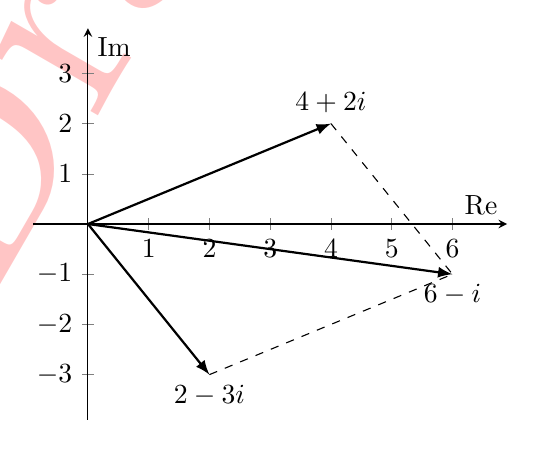
\begin{tikzpicture}
    \begin{axis}[
        xmin = -0.9, xmax = 6.9,
        ymin = -3.9, ymax = 3.9,
        xlabel = Re,
        ylabel = Im,
        xtick distance = 1,
        ytick distance = 1,
    ]
    \draw[thick, -latex] (axis cs: 0, 0) -- (axis cs: 4, 2) node[above] {$4 + 2i$};
    \draw[thick, -latex] (axis cs: 0, 0) -- (axis cs: 2, -3) node[below] {$2 - 3i$};
    \draw[thick, -latex] (axis cs: 0, 0) -- (axis cs: 6, -1) node[below] {$6 - i$};
    \draw[dashed] (axis cs: 4, 2) -- (axis cs: 6, -1);
    \draw[dashed] (axis cs: 2, -3) -- (axis cs: 6, -1);
    \end{axis}
\end{tikzpicture}
\end{center}

Podobnie jak dla liczb rzeczywistych, tak i dla zespolonych można zdefiniować \textbf{moduł} jako odległość od zera w układzie współrzędnych: dla $z = a + bi$ mamy
$$|z| = \sqrt{a^2 + b^2}$$

Dla tak określonego modułu zachodzi również \textbf{nierówność trójkąta}: dla dowolnych $z, w \in \CC$
$$|z + w| \leq |z| + |w|$$

\subsection{Postać trygonometryczna}

Do liczb zespolonych można wprowadzić koncepcję współrzędnych biegunowych -- zamiast określać wektor jako parę współrzędnych $x, y$, będziemy ustalać jego długość i kąt skierowania.

Niech $z=x+iy\in\CC$ i $z\neq0$. Oznaczmy literą $\phi$ kąt pomiędzy półosią rzeczywistą dodatnią i wektorem odpowiadającym $z$ i ustalmy, że jest to kąt zorientowany przeciwnie do ruchu wskazówek zegara. Wówczas $\cos\phi = \frac{x}{|z|}$, $\sin\phi = \frac{y}{|z|}$ oraz
$$
\purple{z = |z|(\cos\phi + i\sin\phi)}
$$
Kąt $\phi$ nazywamy \textbf{argumentem} liczby zespolonej $z$ i oznaczamy $\phi = \arg z$.

\begin{center}
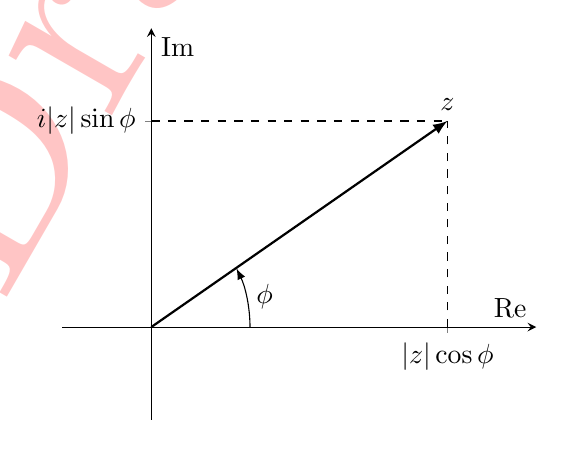
\begin{tikzpicture}
    \begin{axis}[
        xmin = -0.9, xmax = 3.9,
        ymin = -0.9, ymax = 2.9,
        xlabel = Re,
        ylabel = Im,
        xtick = {3},
        ytick = {2},
        xticklabels = {$|z| \cos \phi$},
        yticklabels = {$i |z| \sin \phi$}
    ]
    \draw[thick, -latex] (axis cs: 0, 0) -- (axis cs: 3, 2) node[above] {$z$};
    \draw[dashed] (axis cs: 0, 2) -- (axis cs: 3, 2);
    \draw[dashed] (axis cs: 3, 0) -- (axis cs: 3, 2);
    \draw[-latex] (axis cs: 1, 0) arc [radius = 17mm, start angle = 0, end angle = 26]
        node[right, pos = 0.5] {$\phi$};
    \end{axis}
\end{tikzpicture}
\end{center}

Przy powyższym zapisie, mając $z = |z|(\cos\phi + i\sin\phi)$ i $w = |w|(\cos\theta + i\sin\theta)$, możemy zgrabnie wymnożyć obie liczby:
$$
zw = |z|\cdot|w|(\cos(\phi+\theta)+i\sin(\phi+\theta)).
$$

Widzimy więc, że przy mnożeniu liczb zespolonych ich moduły się mnożą, a argumenty dodają.

\begin{center}
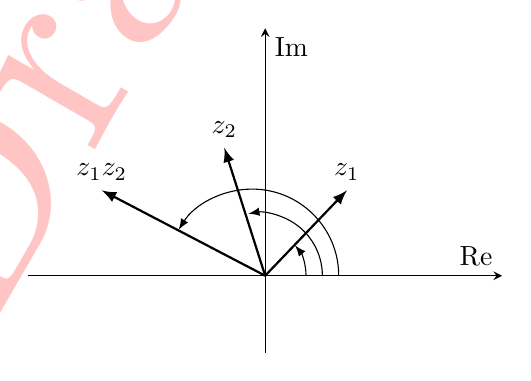
\begin{tikzpicture}
    \begin{axis}[
    	height = 5.7cm,
        xmin = -2.9, xmax = 2.9,
        ymin = -0.9, ymax = 2.9,
        xlabel = Re,
        ylabel = Im,
        xtick = \empty,
        ytick = \empty,
    ]
    \draw[thick, -latex] (axis cs: 0, 0) -- (axis cs: 1, 1) node[above] {$z_1$};
    \draw[-latex] (axis cs: 0.5, 0) arc [radius = 6mm, start angle = 0, end angle = 40];
    \draw[thick, -latex] (axis cs: 0, 0) -- (axis cs: -0.5, 1.5) node[above] {$z_2$};
    \draw[-latex] (axis cs: 0.7, 0) arc [radius = 8mm, start angle = 0, end angle = 100];
    \draw[thick, -latex] (axis cs: 0, 0) -- (axis cs: -2, 1) node[above] {$z_1z_2$};
    \draw[-latex] (axis cs: 0.9, 0) arc [radius = 11mm, start angle = 0, end angle = 148];
    \end{axis}
\end{tikzpicture}
\end{center}

Postać trygonometryczną możemy skrócić do \textbf{zapisu wykładniczego}:
$$
\purple{e^{i\phi} = \cos\phi+i\sin\phi}.
$$
Przy tym zapisie mnożenie liczb zespolonych wygląda prościej:
$$zw = |zw|e^{i(\phi+\theta)}$$

Potęgowanie liczb zespolonych możemy w łatwy sposób wykonać, wykorzystując \textbf{wzór de Moivre'a}:
jeżeli liczba $n$ jest całkowita, natomiast $z=|z|e^{i\phi}=|z|(\cos\phi + i\sin\phi)$, to
$$
\purple{z^n = |z|^ne^{in\phi} = |z|^n(\cos{n\phi} + i\sin{n\phi})}.
$$

\begin{example}
    Obliczymy $(1+i)^{21}$. W postaci trygonometrycznej mamy $1+i=\sqrt{2}(\cos\frac{\pi}{4}+i\sin\frac{\pi}{4})$, zatem
    $$
    (1+i)^{21} = (\sqrt{2})^{21}\left(\cos\frac{21\pi}{4}+i\sin\frac{21\pi}{4}\right) = 2^{10}\sqrt{2}\left(\cos\frac{5\pi}{4}+i\sin\frac{5\pi}{4}\right) = 2^{10}(-1-i)
    $$
\end{example}

\subsection{Pierwiastki zespolone}

Rozpatrzymy rozwiązania równania postaci $x^n = z$, gdzie $z \in \CC \backslash \{0\}$. Każde takie rozwiązanie $x \in \CC$ będziemy nazywać \textbf{pierwiastkiem zespolonym} stopnia $n$ z liczby zespolonej $z$.

Równanie $x^n = z$ ma zawsze $n$ pierwiastków, które są postaci
$$
x_k = \sqrt[n]{|z|} e^{i(\phi+2k\pi)/n} = \sqrt[n]{|z|}\left(\cos\left(\frac{\phi+2k\pi}{n}\right) + i\sin\left(\frac{\phi+2k\pi}{n}\right)\right).
$$

Zwróćmy uwagę, że pierwiastek zespolony to nie liczba, a zbiór liczb. Geometrycznie są one wierzchołkami wielokąta foremnego wpisanego w okrąg o środku w punkcie $(0, 0)$ i promieniu $\sqrt[n]{|z|}$ (dla $n = 2$ otrzymujemy dwa punkty symetryczne względem zera). Wyjaśnienie tego faktu jest intuicyjnie proste: o ile w liczbach rzeczywistych przyjmujemy jako pierwiastki zawsze wartości dodatnie, odrzucając ujemne (np. $\sqrt{9} = 3$, mimo że $(-3)^2$ to też 9), o tyle w liczbach zespolonych nie ma powodu, żeby wyróżniać którykolwiek z pierwiastków.

% TODO: rysunek

Rozpatrzymy jeszcze jeden szczególny przypadek: gdy $z = 1$, otrzymujemy następujący wzór na $n$ różnych zespolonych \textbf{pierwiastków z jedności} stopnia $n$:
$$
x_k = e^{i2k\pi/n} = \cos\left(\frac{2k\pi}{n}\right) + i\sin\left(\frac{2k\pi}{n}\right).
$$

Zauważmy, że wtedy $1 = 1 + 0i$ zawsze jest jednym z pierwiastków. Graficznie wystarczy więc wyznaczyć wierzchołki $n$-kąta foremnego położonego na okręgu o promieniu 1, którego jednym z wierzchołków jest jedynka.

% TODO: rysunek

\begin{editorsnote}
    Do sekcji ,,pierwiastki zespolone'' warto byłoby dodać rysunki.
\end{editorsnote}

\begin{problems}
    \prob Liczba zespolona $x_0$ jest rozwiązaniem równania $x^2 + x + 1 = 0$. Wynika z tego, że
    \answers{liczba $x_0^2$ też jest rozwiązaniem tego równania}{liczba $1/x_0$ też jest rozwiązaniem tego równania}{$x_0^3 = 1$}

    \prob Strukturę grupy z działaniem mnożenia liczb zespolonych i 1 jako elementem neutralnym ma zbiór
    \answers{$\{2^kz \in \CC \ : \; z^{2019} = 1\}$}{$\{z \in \CC \ : \; \Re(z) \cdot \Im(z) = 0\}$}{$\{z \in \CC \ : \ k \in \ZZ, \ |z| = 1\}$}
\end{problems}

\section{Przestrzenie liniowe}

Aby móc odpowiednio wprowadzić intuicję stojącą za przestrzeniami liniowymi, zaczniemy od ujednolicenia pojęcia \textbf{wektora}. Rozważając zagadnienia algebry liniowej umawiamy się, że \purple{punktem przyłożenia każdego z rozważanych wektorów jest zero} (o zadanym wymiarze, a więc może to być np. $(0, 0), (0, 0, 0)$ itd.).

Ponadto, w wielu przypadkach będziemy \purple{utożsamiać pojęcie punktu z pojęciem wektora}, tzn. punkt $(x, y)$ będziemy intuicyjnie kojarzyć z wektorem o początku w zerze i końcu w punkcie $(x, y)$. W związku z tym współrzędne wektora zapisujemy czasem w nawiasach okrągłych (jak w przypadku punktu) i nie zawsze używamy notacji nawiasów kwadratowych.

\begin{example}
	Punkt $(3, 2)$ można utożsamiać z wektorem $(3, 2)$, co pokazuje poniższy rysunek.
	
	\begin{center}
	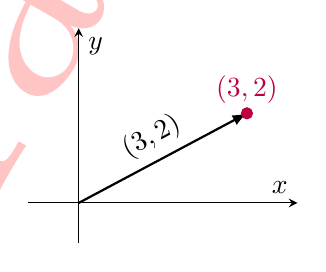
\begin{tikzpicture}
		\begin{axis}[
			width = 5cm,
			xmin = -0.9, xmax = 3.9,
			ymin = -0.9, ymax = 3.9,
			xtick = \empty,
			ytick = \empty,
			]
			\draw[thick, -latex] (axis cs: 0, 0) -- (axis cs: 3, 2)
				node[above, pos = 0.5, sloped] {$(3, 2)$};
                \draw[purple, fill] (axis cs: 3, 2) circle (2pt)
				node[above] {$(3, 2)$};
		\end{axis}
	\end{tikzpicture}
	\end{center}
\end{example}

Oznaczmy przez $\KK$ pewne ciało i przez $V$ zbiór pewnych wektorów, taki że $(V, +, 0)$ jest grupą abelową. Załóżmy też, że w zbiorze $X$ określone jest działanie ,,$\cdot$'' mnożenia wektora $\vec{v} \in V$ przez skalar $a \in \KK$, przy czym spełnia ono następujące własności: dla dowolnych $a, b \in \KK$ i $\vec{v}, \vec{w} \in V$
\begin{itemize}
	\item mnożenie przez skalar jest rozdzielne względem dodawania wektorów:
	$$a(\vec{v} + \vec{w}) = a\vec{v} + a\vec{w},$$
	
	\item mnożenie przez wektor jest rozdzielne względem dodawania skalarów:
	$$(a + b)\vec{v} = a\vec{v} + b\vec{v},$$
	
	\item dwukrotne mnożenie wektora przez skalar można zastąpić mnożeniem skalarów:
	$$a \cdot (b \cdot \vec{v}) = (a \cdot b) \cdot \vec{v},$$
	
	\item elementem neutralnym mnożenia przez skalar jest element neutralny mnożenia skalarów $1 \in \KK$:
	$$1 \cdot \vec{v} = \vec{v}.$$
\end{itemize}

Wówczas zbiór $V$ wraz z tak zdefiniowanymi działaniami ,,$+$'' i ,,$\cdot$'' jest \textbf{przestrzenią liniową} nad ciałem $\KK$. Elementy przestrzeni liniowej nazywamy wektorami, a ciała $\KK$ -- skalarami.

\begin{example}
	Oto kilka przykładów przestrzeni liniowych (oraz struktur, które przestrzeniami liniowymi nie są):
	
	\begin{itemize}
		\item Standardowa przestrzeń rzeczywistych wektorów $n$-wymiarowych $\RR^n$ jest, w oczywisty sposób, przestrzenią liniową nad $\RR$. Nie jest ona jednak przestrzenią liniową nad $\CC$, gdyż np. mamy $i \cdot (1, 1) = (i, i)$ -- pomnożenie wektora z $\RR^n$ przez skalar z $\CC$ sprawia, że opuszczamy przestrzeń wektorów rzeczywistych.
		
		\item Ogół funkcji wielomianowych jednej zmiennej rzeczywistej $x$ o współczynnikach rzeczywistych $\RR[x]$ jest przestrzenią liniową nad $\RR$. Przykładowo, $x^2 + 1$ oraz $2x^3 + 5x^2 + 3$ są wektorami tej przestrzeni. Możemy je do siebie dodawać i mnożyć przez rzeczywiste skalary, a działania te spełniają wszystkie warunki wymagane w definicji przestrzeni liniowej.
		
		\item Wektory z $\RR^2$ postaci $\{(2a, a) \ | \ a \in \RR\}$ rozpinają przestrzeń liniową. Gdybyśmy narysowali zbiór punktów tożsamych z tymi wektorami, uzyskalibyśmy prostą przechodzącą przez $(0, 0)$. Nie jest jednak prawdą, że punkty z dowolnej prostej utworzą przestrzeń wektorową. Na przykład, punkty z prostej o równaniu $y = x + 1$ są postaci $(x, x + 1)$ i nie tworzą przestrzeni wektorowej, gdyż m.in. punkty $(0, 1)$ i $(1, 2)$ do niej należą, a ich suma $(1, 3)$ -- już nie.
	\end{itemize}
\end{example}

Jak widać, wektorami mogą być obiekty dość dalekie od definicji ze szkoły średniej (czyli przestrzeni $\RR^n$). Takie ogólne podejście pozwoli przenosić wiele ciekawych zależności ze standardowego $\RR^n$ do innych struktur.
\bigskip

Fakt istnienia w przestrzeniach liniowych \textbf{wektora i skalara zerowego} definiuje nam kilka dodatkowych własności: jeżeli $V$ jest przestrzenią liniową nad ciałem $\KK$, to dla każdego wektora $\vec{v} \in V$ oraz skalara $a \in \KK$ zachodzą zależności:
\begin{itemize}
    \item $0 \cdot \vec{v} = a \cdot \vec{0} = 0$ (gdzie ,,$0$'' po lewej to zero w ciele $\KK$, a ,,$\vec{0}$'' po prawej to element neutralny dodawania w $V$),
    \item $a\vec{v} = \vec{0} \wtw a = 0 \ \lor \ \vec{v} = \vec{0}$,
    \item $(-a)\vec{v} = a(-\vec{v}) = -(a\vec{v})$, gdzie przez $-\vec{v} \in V$ rozumiemy wektor przeciwny do $\vec{v}$.
\end{itemize}

\subsection{Podprzestrzenie liniowe}

Załóżmy, że $V$ jest przestrzenią liniową nad ciałem $\KK$ i $P \subset V$ jest jej niepustym podzbiorem, który, wraz z odziedziczonymi z $V$ działaniami dodawania i mnożenia przez skalar, także jest przestrzenią liniową nad $\KK$. Mówimy wówczas, że $P$ jest \textbf{podprzestrzenią liniową} przestrzeni $V$.

\begin{example}
	Weźmy przestrzeń $\RR^2$ nad $\RR$. Jej przykładową podprzestrzenią jest zbiór $\{(3a, 5a) \ | \ a \in \RR\}$. Z kolei przykładową podprzestrzenią tej przestrzeni jest $\{\vec{0}\}$ -- podprzestrzeń jednoelementowa, składająca się wyłącznie z wektora zerowego.
\end{example}

Prawdą jest, że $P \neq \pusty$ jest podprzestrzenią liniową $V$ wtedy i tylko wtedy, gdy zachodzą wszystkie z poniższych warunków:
\begin{itemize}
	\item $\vec{0} \in P$
    \item dla dowolnych $\vec{v}, \vec{w} \in P$ także $\vec{v} + \vec{w} \in P$,
    \item dla dowolnych $\vec{v} \in P$ i $a \in \KK$ także $a \vec{v} \in P$.
\end{itemize}

\subsection{Liniowa niezależność}

Załóżmy, że $V$ jest przestrzenią liniową nad ciałem $\KK$. \textbf{Kombinacją liniową wektorów} $\vec{v_1}, ..., \vec{v_n} \in V$ o współczynnikach $a_1, ..., a_n \in \KK$ nazywamy każdy z wektorów postaci
$$\vec{v} = a_1\vec{v_1} + ... + a_n\vec{v_n}.$$

\begin{example}
    Każdy wektor $\vec{v} \in \RR^3$ jest kombinacją liniową wektorów jednostkowych $\vec{e_1} = (1, 0, 0), \vec{e_2} = (0, 1, 0), \vec{e_3} = (0, 0, 1)$:
    $$\vec{v} = (a_1, a_2, a_3) = a_1\vec{e_1} + a_2\vec{e_2} + a_3\vec{e_3}$$
\end{example}

Niech $V$ będzie przestrzenią liniową, natomiast $G \subset V$ pewnym zbiorem wektorów. Najmniejszą podprzestrzeń liniową zawierającą wszystkie wektory z $G$ nazywamy \textbf{podprzestrzenią rozpiętą} przez $G$ i oznaczamy jako
$\purple{\spn{G}}$. Jeżeli $G = \{\vec{g_1}, ..., \vec{g_k}\}$, to
$$\purple{\spn{G} = \{a_1\vec{g_1} + ... + a_k\vec{g_k} \ | \ a_1, ..., a_k \in \KK\}}$$

Podprzestrzenie rozpięte przez pewien zbiór wektorów składają się więc ze wszystkich kombinacji liniowych wektorów z tego zbioru.

\begin{example}
    Weźmy przestrzeń funkcji wielomianowych $\RR[x]$. Wtedy $\spn{\{1, x^2\}}$ to ogół wielomianów postaci $w(x) = ax^2 + b$, gdzie $a, b \in \RR$. Z kolei $\spn{\{1, x^2 + 1\}}$ to ogół wielomianów postaci $w(x) = c(x^2 + 1) + d$, gdzie $c, d \in \RR$, czyli tak naprawdę ogół wielomianów postaci $w(x) = ax^2 + b$ -- taka zmiana zbioru rozpinającego przestrzeń nie dała w tym wypadku niczego nowego.
    
    A czym jest $\spn{\{x^2 + 1\}}$? To zbiór wszystkich wielomanów postaci $ax^2 + a$ dla $a \in \RR$. Jest on mniejszy niż poprzedni (tzn. poprzedni ma wszystkie występujące tu wielomiany i jeszcze jakieś inne, np. $x^2 + 2$).
\end{example}

\begin{example}
	Pozostańmy w przestrzeni $\RR[x]$. Tym razem weźmy jednak nieskończony zbiór rozpinający przestrzeń: $G = \{1, x, x^2, x^3, ...\}$. Widać, że w $\spn{G}$ znajdą się wszystkie wielomiany, a ponieważ wielomiany są podprzestrzenią, w $\spn{G}$ nie będzie nic więcej. Może trochę dziwić fakt, że choć np. $2x^3 + 5x^2 - 7x + 4 \in \spn{G}$, to $1 + x + x^2 + x^3 + ... \notin \spn{G}$ -- weźmy jednak pod uwagę, że w podprzestrzeniach rozpiętych mamy jedynie skończone sumy przeskalowanych wektorów bazowych.
\end{example}

\begin{example}
	Rozważmy przestrzeń $\RR^3$ i weźmy zbiór jednoelementowy $\{(1, 2, 3)\}$. Wtedy $$\spn{\{(1, 2, 3)\}} = \{a(1, 2, 3) \ | \ a \in \RR\},$$ czyli podprzestrzenią rozpiętą jest zbiór wszystkich przeskalowań wektora $(1, 2, 3)$, a więc wektory $$(0, 0, 0), (1, 2, 3), (2, 4, 6), (0.5, 1, 1.5), (-1, -2, -3) \ \text{itd.}$$ Geometrycznie będzie to prosta w $\RR^3$ przechodząca przez punkt $(0, 0, 0)$.
	
	Dodajmy teraz wektor $(2, 0, 3)$, otrzymując $$\spn{\{(1, 2, 3), (2, 0, 3)\}} = \{a(1, 2, 3) + b(2, 0, 3) \ | \ a, b \in \RR\}.$$ Ustalając $b = 0$ i wstawiając wszystkie możliwe $a$, wygenerujemy tę samą prostą, co poprzednio. Dla innych wartości $b$ otrzymamy inne proste, równoległe do siebie wzajemnie. Wszystkie te proste biegną w tym samym kierunku co wektor $(2, 0, 3)$, więc łącząc je wszystkie w całość dochodzimy do wniosku, że nasza przestrzeń $\spn{\{(1, 2, 3), (2, 0, 3)\}}$ to pewna płaszczyzna umieszczona w $\RR^3$ (złożona ze wszystkich powstałych prostych).
	
	A co ze $\spn{\{(1, 2, 3), (2, 0, 3), (-1, 2, -2)\}}$? Dodanie wektora $(-1, 2, -2)$ nie zmieni naszej przestrzeni -- wystarczy zauważyć, że $$(-1, 2, -2) = (1, 2, 1) + (-1)(2, 0, 3),$$ więc z pomocą $(-1, 2, -2)$ nie wygenerujemy żadnych nowych kombinacji liniowych.
\end{example}

Rozważając powyższe przykłady, zajmiemy się teraz kwestią zbędnych generatorów, czyli takich wektorów, których dodanie do zbioru rozpinającego przestrzeń nie ma żadnego wpływu na otrzymaną przestrzeń. Nietrudno zauważyć, że jeśli pewien wektor jest kombinacją liniową pozostałych wektorów, to można go odrzucić, gdyż nic nowego nie wniesie.

Zbiór wektorów nazywamy zbiorem wektorów \textbf{liniowo zależnych}, jeśli pewien element tego zbioru można przedstawić jako kombinacją liniową pewnych pozostałych.

Natomiast układ wektorów niespełniający powyższego warunku jest \textbf{liniowo niezależny}. Formalnie, ma on więc następującą własność: dla dowolnych $a_1, ..., a_n \in \KK$ zachodzi
$$a_1\vec{v_1} + ... + a_n\vec{v_n} = 0 \ \Leftarrow \ a_1 = ... = a_n = 0$$

\begin{example}
	Liniowo niezależny jest zbiór wektorów $\{(1, 0, 0), (1, 1, 0), (1, 1, 1)\}$ -- nie da się otrzymać żadnego z wektorów poprzez kombinację liniową pozostałych.
	
	Natomiast zbiór
	$$\{(1, 0, 0), (1, 1, 0), (1, 1, 1), (5, 6, 7)\}$$
	jest liniowo zależny, bo na przykład
	$$(5, 6, 7) = 7 \cdot (1, 1, 1) - (1, 1, 0) - (1, 0, 0)$$
\end{example}

Intuicyjnie, o liniowej niezależności możemy myśleć w następujący sposób: każdy wektor w zbiorze liniowo niezależnym niesie ze sobą \textit{pewną unikalną informację}, której nie da się uzyskać za pomocą pozostałych wektorów w tym zbiorze.

Przytoczymy jeszcze jeden ważny fakt: \purple{dowolny podzbiór zbioru wektorów liniowo niezależnych także jest liniowo niezależny}.

\subsection{Baza i wymiar przestrzeni liniowej}

Jeszcze raz przyjrzymy się kwestii zbędnych generatorów przestrzeni rozpiętych. Wiemy już, że kluczowa jest tu cecha liniowej niezależności zbioru rozpinającego przestrzeń.

Układ wektorów $\vec{v_1}, ..., \vec{v_n} \in V$ nazywamy \textbf{bazą} przestrzeni $V$, jeżeli jest on liniowo niezależny i rozpina przestrzeń $V$ (tj. $V = \spn{\{\vec{v_1}, ..., \vec{v_n}\}}$).

Co ważne, każdy wektor z przestrzeni \purple{zapisuje się dokładnie na jeden sposób} jako kombinacja liniowa wektorów z bazy tej przestrzeni. Intuicyjnie więc baza stanowi zbiór wektorów, z których ,,budujemy'' całą przestrzeń bazową (tj. wszystkie jej elementy).

Baza jest zarówno maksymalnym układem wektorów liniowo niezależnych w swojej przestrzeni, jak i minimalnym zbiorem wektorów rozpinających daną przestrzeń. Jak należy to rozumieć?
\begin{itemize}
	\item \purple{Każdy właściwy podzbiór bazy jest zbiorem liniowo niezależnym, rozpinającym pewną podprzestrzeń bazowej przestrzeni.} Intuicyjnie: skoro baza składa się z wektorów liniowo niezależnych, to usunięcie z niej dowolnego elementu zabiera nam \textit{pewną unikalną informację}, którą ten element wnosił. Co za tym idzie -- nie będziemy w stanie wygenerować (za pomocą kombinacji liniowych pozostałych elementów) niektórych elementów z bazowej przestrzeni, do których otrzymania był niezbędny usunięty przez nas element. Taki podzbiór bazy rozepnie więc pewną, mniejszą podprzestrzeń bazowej przestrzeni.
	
	\item \purple{Każdy właściwy nadzbiór bazy jest zbiorem liniowo zależnym.} Skoro baza rozpina całą przestrzeń, tj. nie ma w niej elementów, których nie dałoby się uzyskać poprzez kombinację liniową wektorów z bazy, to dodanie jakiegokolwiek elementu nie może przynieść nam już żadnej dodatkowej informacji, która pozwoliłaby nam uzyskać nowe elementy (bo takie nie istnieją). Mamy więc pewność, że każdy dodany do bazy element jest kombinacją liniową wektorów z bazy.
\end{itemize}

\begin{example}
    Rozważmy przestrzeń $\RR^3$ i jej \textbf{bazę kanoniczną} (tzn. złożoną z wektorów jednostkowych):
    $$\{(1, 0, 0), (0, 1, 0), (0, 0, 1)\}$$
   	Nietrudno sprawdzić, że rzeczywiście jest to baza: jej wektory są w oczywisty sposób liniowo niezależne, a każdy wektor z $\RR^3$ można zapisać jako liniową kombinację wektorów bazowych:
   	$$(a, b, c) = a(1, 0, 0) + b(0, 1, 0) + c(0, 0, 1)$$
   	
   	Inną przykładową bazą przestrzeni $\RR^3$ jest
   	$$\{(1, 0, 0), (7, 7, 0), (42, 42, 42)\}.$$
\end{example}

Z przedstawionych powyżej dwóch faktów możemy wywnioskować, że wszystkie bazy danej przestrzeni składają się z tej samej liczby wektorów. Tę liczbę nazywamy \textbf{wymiarem} przestrzeni liniowej $V$ i oznaczamy przez $\purple{\dim V}$. Jeżeli $V$ nie ma bazy skończonej, przyjmujemy $\dim V = \infty$.

\begin{example}
    Oto kilka przykładów wymiarów baz różnych przestrzeni:
    \begin{itemize}
    	\item Każda z przestrzeni $\RR^n$ dla $n \in \NN_+$ ma wymiar $n$, gdyż np. jej baza kanoniczna liczy właśnie $n$ elementów ($n$ wektorów bazowych, po jednym na każdą z $n$ współrzędnych wektora).
    	
    	\item Podprzestrzeń zerowa $\{(0, 0, 0)\}$ przestrzeni $\RR^3$ ma wymiar równy 0.
    	
    	\item Przestrzeń funkcji wielomianowych zmiennej rzeczywistej stopnia co najwyżej 2 o współczynnikach rzeczywistych ma wymiar 3, gdyż jej baza kanoniczna $\{1, x, x^2\}$ liczy właśnie 3 elementy.
    	
    	\item Przestrzeń $\RR[x]$ ma wymiar równy $\infty$ -- skończona baza nie pozwoliłaby bowiem zapisywać wielomianów odpowiednio wysokich stopni.
    \end{itemize}
\end{example}

Z pojęciem wymiaru związane są bardzo ważne własności.

Załóżmy, że $\dim{V} < \infty$ i $U \subseteq V$ jest podprzestrzenią liniową $V$. Wówczas
\begin{itemize}
	\item $\dim{U} \leq \dim{V}$,
	\item $\dim{U} = \dim{V}$ wtedy i tylko wtedy, gdy $U = V$.
\end{itemize}

Załóżmy, że $\dim{X}=n<\infty$. Wówczas
\begin{itemize}
    \item każdy liniowo niezależny układ wektorów z $X$ można uzupełnić do bazy przestrzeni $X$,
    \item z każdego układu wektorów rozpinających przestrzeń $X$ można wybrać bazę przestrzeni $X$,
    \item jeżeli pewne $n$ wektorów $x_1,\ldots,x_n\in X$ jest liniowo niezależne, to są one bazą przestrzeni $X$,
    \item jeżeli pewne $n$ wektorów $x_1,\ldots,x_n\in X$ rozpina przestrzeń $X$, to są one jej bazą.
\end{itemize}

\subsection{Przecięcie i suma podprzestrzeni}

Załóżmy, że $X$ jest przestrzenią liniową nad ciałem $\KK$ i $Y_j\subset X$ są podprzestrzeniami liniowymi, gdzie $j\in J$. Wówczas zbiór będący \textbf{przecięciem} tych przestrzeni,
$$
Y = \bigcap_{j\in J}Y_j,
$$
też jest podprzestrzenią liniową w $X$.

\begin{example}
    Przecięciem podprzestrzeni $U = \{ x \in \RR^3 : x_1 + x_2 = 0\}, V = \{x \in \RR^3 : x_2 + x_3 = 0\}$ jest
    $$U \cap V = \spn\big\{(1, -1, 1)\big\} \subset \RR^3$$
\end{example}

Załóżmy, że $X$ jest przestrzenią liniową nad ciałem $\KK$ i $U,V\subset X$ są podprzestrzeniami liniowymi. \textbf{Suma} podprzestrzeni $U$ i $V$ to zbiór
$$
U + V = \{u+v\in X : u\in U, v\in V\}.
$$
Taka suma podprzestrzeni też jest podprzestrzenią liniową w $X$.

W ogólności nie jest prawdą, że $U+V=U\cup V$. Łatwo widać, że $U\cup V\subset U+V$. Ponadto, zbiór $U\cup V$ nie musi być podprzestrzenią liniową w $X$.

Następujące warunki są równoważne:
\begin{itemize}
    \item $U\cap V=\{0\}$,
    \item dla każdego wektora $x\in U+V$ wektory $u\in U$ i $v\in V$ takie, że $x=u+v$ są wyznaczone jednoznacznie.
\end{itemize}

\begin{example}
    W przestrzeni wielomianów 3 stopnia o współczynnikach rzeczywistych $\RR[x]_3$ zachodzi
    $$\spn(1, x^2) + \spn(1 + x, x^2 + x^3) = \spn(1, x, x^2, x^3) = \RR[x]_3$$
\end{example}

Załóżmy, że $X$ jest przestrzenią liniową nad ciałem $\KK$ i $U,V\subset X$ są podprzestrzeniami liniowymi. Jeśli $U$ i~$V$ są rozłączne (tj. $U\cap V=\{0\}$), mówimy, że podprzestrzeń $U+V$ jest \textbf{sumą prostą} podprzestrzeni $U$ i~$V$ i~piszemy $U+V=\purple{U\oplus V}$.

\begin{example}
    W przestrzeni wielomianów 3 stopnia o współczynnikach rzeczywistych $\RR[x]_3$ zachodzi
    $$\spn(1, x^2) \oplus \spn(x, x^3) = \spn(1, x, x^2, x^3) = \RR[x]_3$$
\end{example}

Jeżeli $Y,Z\subset X$ są podprzestrzeniami skończonego wymiaru, to
\begin{itemize}
    \item wymiary podprzestrzeni $Y\cap Z$ oraz $Y+Z$ też są skończone,
    \item $\purple{\dim(Y+Z)=\dim{Y}+\dim{Z}-\dim(Y\cap Z)}$.
\end{itemize}

\begin{problems}
    \prob Niech $X$ będzie przestrzenią liniową wymiaru 15. Wynika z tego, że
    \answers{każdy układ 20 wektorów z $X$ jest liniowo zależny}{każdy układ 10 wektorów z $X$ jest liniowo niezależny}{każda baza $X$ składa się z 15 wektorów}

    \prob Dana jest przestrzeń $X$ wymiaru 10 oraz podprzestrzenie $U$, $V$, takie że $\dim(U) = \dim(V)$ oraz $X = U + V$. Wynika z tego, że
    \answers
    {$\dim(U) = 5$}
    {$\dim(U) \geq 5$}
    {$\dim(U \cap V) = 0$}
    
    \prob Dane są elementy przestrzeni liniowej nad ciałem liczb rzeczywistych $\Vec{a}, \Vec{b}, \Vec{c}$. Prawdą jest, że
    \answers{jeżeli $(\Vec{a}, \Vec{b}, \Vec{c})$ jest niezależny liniowo, to $(\Vec{a} - \Vec{b}, \Vec{b} - \Vec{c}, \Vec{c} - \Vec{a})$ jest niezależny liniowo}{jeżeli $(\Vec{a}, \Vec{b}, \Vec{c})$ jest niezależny liniowo, to $(\Vec{a} + \Vec{b}, \Vec{b} + \Vec{c}, \Vec{c} + \Vec{a})$ jest niezależny liniowo}{jeżeli $(\Vec{a} + \Vec{b}, \Vec{b} + \Vec{c}, \Vec{c} + \Vec{a})$ jest niezależny liniowo, to $(\Vec{a}, \Vec{b}, \Vec{c})$ jest niezależny liniowo}
\end{problems}

\section{Macierze i przekształcenia liniowe}

\textbf{Macierzą} (nad ciałem $\KK$) wymiaru $m \times n$ nazywamy tablicę prostokątną 
$$
\begin{bmatrix}
    a_{1,1} & a_{1,2} & \cdots & a_{1,n} \\
    a_{2,1} & a_{2,2} & \dots & a_{2,n} \\
    \vdots & \vdots & \ddots & \vdots \\
    a_{m,1} & a_{m,2} & \cdots & a_{m,n}     
\end{bmatrix}
$$
gdzie $a_{i,j} \in \KK$ dla $1 \leq i \leq m, \ 1 \leq j \leq n$. Można też zapisać taką macierz jako $$
A=[a_{i,j}]_{i=1,\dots,m, \ j=1,\dots,n}
$$
Macierz $m\times n$ ma $m$ wierszy i $n$ kolumn. \purple{Pierwszy indeks odpowiada wierszowi, a drugi kolumnie}. Piszemy wtedy, że macierz należy do zbioru macierzy $\KK^{m, n}$.

Specyficznym przypadkiem macierzy jest macierz $\KK^{n, 1}$ lub po prostu macierz $\KK^n$, którą nazywamy \textbf{wektorem} długości $n$:
$$
\vec{x} = \begin{bmatrix}
    x_1 \\ x_2 \\ \dots \\ x_n
\end{bmatrix}
$$

Przykłady innych często spotykanych macierzy:
\begin{itemize}
    \item \textbf{macierz zerowa} -- jej elementy to same zera,
    \item \textbf{macierz diagonalna} -- macierz kwadratowa zawierająca niezerowe wartości jedynie na diagonali (przekątnej), zapisujemy $D=\text{diag}(d_1,\dots, d_n)$,
    \item \textbf{macierz jednostkowa} rozmiaru $n \times x$, taka że $I_n=\text{diag}(1, \dots, 1)$,
    \item \textbf{macierz górno- i dolnotrójkątna} -- zawierająca niezerowe wartości jedynie na diagonali oraz ponad/poniżej niej,
    \item \textbf{macierz permutacji} -- macierz kwadratowa, która ma w każdym wierszu i w każdej kolumnie dokładnie jedną jedynkę oraz zera na pozostałych miejscach.
\end{itemize}

\subsection{Działania na macierzach}
Niech 
$$
A=\begin{bmatrix}
    a_{1,1} & a_{1,2} & \cdots & a_{1,n} \\
    a_{2,1} & a_{2,2} & \cdots & a_{2,n} \\
    \vdots & \vdots & \ddots & \vdots \\
    a_{m,1} & a_{m,2} & \cdots & a_{m,n}    
\end{bmatrix} \ \in \KK^{m,n}
$$
\textbf{Transpozycją macierzy} $A\in\KK^{m,n}$ nazywamy macierz
$$
A^T=\begin{bmatrix}
    a_{1,1} & a_{2,1} & \cdots & a_{m,1} \\
    a_{1,2} & a_{2,2} & \cdots & a_{m,2} \\
    \vdots & \vdots & \ddots & \vdots \\
    a_{1,n} & a_{2,n} & \cdots & a_{m,n}    
\end{bmatrix} \ \in \KK^{n,m}
$$
o zamienionych kolumnach z wierszami (dla macierzy niekwadratowych zmieniają się także wymiary macierzy). Macierz $A$ jest \textbf{symetryczna} jeśli zachodzi $A=A^T$ oraz \textbf{antysymetryczna} jeśli $A=-A^T$.

\textbf{Hermitowskie sprzężenie} macierzy $A$ to jej transpozycja wraz ze sprzężeniem każdego z jej elementów, na przykład
$$
\begin{bmatrix}
    1+i & 2 & 2 - i \\
    2 + 3i  & i & 0 \\
\end{bmatrix}^H = 
\begin{bmatrix}
    1 - i & 2 - 3i \\
    2 & -i \\
    2 + i & 0
\end{bmatrix}
$$
i, jak widać, $A^H=\overline{A^T}=(\overline{A})^T$. Macierz $A$ jest hermitowska, gdy $A=A^H$.

\textbf{Dodawanie i odejmowanie macierzy} określone jest \purple{jedynie dla macierzy o tych samych wymiarach} -- odpowiadające sobie elementy (o tych samych indeksach) należy dodać lub odjąć i utworzyć w ten sposób macierz wynikową.

\textbf{Mnożenie macierzy} $A$ z macierzą $B$ jest zdefiniowane jedynie, gdy \purple{$A$ jest wymiarów $m\times k$ oraz $B$ jest wymiarów $k \times n$}, czyli macierz po lewej musi mieć tyle kolumn, ile ta po prawej ma wierszy. Widać to, gdy zapiszemy macierze w sposób wygodny do mnożenia:

$$
\hspace{6em} \begin{bmatrix}
    1 & -1 & 1 & 2 \\
    2 & 0 & 1 & 3 \\
    3 & 1 & 1 & 4
\end{bmatrix}
$$
$$
\begin{bmatrix}
    1 & -1 & 2 \\
    0 & 3 & -2
\end{bmatrix}\cdot = 
\begin{bmatrix}
    5 & 1 & 2 & 13 \\
    0 & -2 & 1 & -17
\end{bmatrix}
$$

Własności mnożenia macierzy ($A, B, C$ są macierzami takimi, że odpowiednie działania są zdefiniowane, $c$~jest skalarem):
\begin{itemize}
    \item $(A + B)\cdot C = A\cdot C + B \cdot C$
    \item $A\cdot(B+C)=A\cdot B + A\cdot C$
    \item $c(A\cdot B) = cA \cdot B = A \cdot cB$
    \item $(A\cdot B)\cdot C = A\cdot(B\cdot C)$
    \item $(A\cdot B)^T = B^T\cdot A^T$
    \item jeśli $A$ to macierz zerowa, to $A\cdot B$ też jest zerowa
    \item $A\cdot B$ niekoniecznie wynosi $B\cdot A$, dla macierzy niekwadratowych nie jest w ogóle określone
    \item jeśli $A\cdot B = [0]_{m,n}$, to niekoniecznie $A$ lub $B$ muszą być macierzami zerowymi
\end{itemize}

Macierz kwadratowa $A \in \KK^{n,n}$ jest \textbf{nieosobliwa} (odwracalna), gdy istnieje macierz kwadratowa $A^{-1} \in \KK^{n,n}$ \textit{odwrotna} do niej, taka że $A \cdot A^{-1} = A^{-1} \cdot A = I_n$. Tylko dla macierzy kwadratowych istnieją macierze odwrotne.

\subsection{Wyznacznik macierzy}
Oznaczmy jako $A_{i,j} \in \KK^{n-1, n-1}$ macierz otrzymaną z macierzy $A \in \KK^{n, n}$ poprzez usunięcie $i$-tego wiersza i~$j$-tej kolumny. Niech $n=1,2,3,\dots$ oraz $A=[a_{i,j}]_{i,j=1}^n\in\KK^{n,n}$. \textbf{Wyznacznik} stopnia $n$ to funkcja \purple{$\det = \det_n:\KK^{n,n}\to \KK$} zdefiniowana w następujący sposób:
\begin{itemize}
    \item dla $n=1$: $\det_1[a_{1,1}]=a_{1,1}$,
    \item dla $n>1$: $\det_nA=\sum_{i=1}^n(-1)^{i+1}a_{i,1}\cdot \det_{n-1}A_{i,1}$ -- rozwinięcie Laplace'a.
\end{itemize}

\begin{example}
    Obliczymy wyznacznik macierzy o wymiarach $2 \times 2$ za pomocą rozwinięcia Laplace'a: jeśli $A = \begin{bmatrix}
        a & b \\ c & d
    \end{bmatrix}$, to
    $$\det A = \det_2 A = a \cdot \det_1 \Vect{d} - c \cdot \det_1 \Vect{b} = ad - bc$$
\end{example}

Przy liczeniu wyznaczników przydaje się także \textbf{twierdzenie Cauchy'ego}: jeżeli $A,B\in \KK^{n,n}$, to 
$$
\purple{\det_n(AB)=\det_n(A)\cdot \det_n(B)}.
$$

Rozważymy teraz \textbf{interpretację geometryczną wyznacznika}: odpowiada ona temu, jak macierz jako przekształcenie liniowe (o tym więcej w następnym dziale) \purple{skaluje pole powierzchni} przypadające na dany jej fragment:
\begin{figure}[H]
    \centering
    \includegraphics[scale=0.2]{rozdziały/images/GAL/3b1b_1.png}
\end{figure}
macierz $\begin{bmatrix}
    3 & 0 \\ 0 & 2
\end{bmatrix}$ przekształca kwadrat o wymiarach $1\times 1$ na prostokąt o wymiarach $3\times 2$, więc jej wyznacznik jest równy 6 (pole obszaru wzrosło sześciokrotnie),
\begin{figure}[H]
    \centering
    \includegraphics[scale=0.2]{rozdziały/images/GAL/3b1b_2.png}
\end{figure}
a macierz $\begin{bmatrix}
    1 & 1 \\ 0 & 1
\end{bmatrix}$ ma wyznacznik $1$: chociaż zmienia ona ułożenie układu współrzędnych, widać, że początkowy kwadrat zmienił się jedynie w romb o takim samym polu powierzchni.
\begin{figure}[H]
    \centering
    \includegraphics[scale=0.2]{rozdziały/images/GAL/3b1b_3.png}
\end{figure}
Z tą wiedzą nietrudno zauważyć, że wyznacznik macierzy odwrotnej musi wynosić $\purple{\det(A^{-1})=\frac{1}{\det(A)}}$. Skoro macierz odwrotna cofa zmiany wprowadzone na układzie współrzędnych, w szczególności musi przywrócić pole początkowego kwadratu do pierwotnej powierzchni.

\subsection{Obraz, jądro i rząd macierzy}

\textbf{Obrazem macierzy} $A\in\KK^{m,n}$ nazywamy zbiór wektorów, które mogą powstać przez przemnożenie ich przez macierz $A$:
$$
\purple{\im A= \{A\vec{x}\in \KK^m \ : \ x \in \KK^n \}}
$$
Obraz macierzy jest podprzestrzenią liniową w $\KK^m$ \purple{rozpiętą przez jej kolumny}.

\begin{example}
    Wyznaczymy obraz macierzy $A=\begin{bmatrix} 1 & 2 & 0 \\ -1 & 1 & -3 \\ 1 & 0 & 2 \end{bmatrix} \in \RR^{3,3}$. Weźmy dowolny wektor $\vec{x}=[x_1,x_2,x_3]^T\in\RR^3$. Wtedy
    $$
    \begin{bmatrix}
        1 & 2 & 0 \\
        -1 & 1 & -3 \\
        1 & 0 & 2 
    \end{bmatrix} \begin{bmatrix}
        x_1 \\ x_2 \\ x_3
    \end{bmatrix} = x_1 \begin{bmatrix}
        1 \\ -1 \\ 1
    \end{bmatrix} + x_2 \begin{bmatrix}
        2 \\ 1 \\ 0
    \end{bmatrix} + x_3 \begin{bmatrix}
        0 \\ -3 \\ 2
    \end{bmatrix}.
    $$
    Zatem
    $$
    \im A = \spn \left(
    \begin{bmatrix}
        1 \\ -1 \\ 1
    \end{bmatrix},
     \begin{bmatrix}
        2 \\ 1 \\ 0
    \end{bmatrix} ,
    \begin{bmatrix}
        0 \\ -3 \\ 2
    \end{bmatrix}
    \right).
    $$
\end{example}

\textbf{Jądrem macierzy} $A \in \KK^{m, n}$ nazywamy zbiór tych wektorów, które przemnożone przez macierz $A$ stają się wektorem zerowym:
$$
\purple{\ker A = \{\vec{x} \in \KK^n \ : \ A\vec{x}=\vec{0}  \}}.
$$
Jądro macierzy jest podprzestrzenią liniową w $\KK^n$.
\bigskip

\textbf{Rząd macierzy} $A\in\KK^{m,n}$ to liczba $\purple{\rank A=\dim(\im A)}$. Zachodzą równości $\rank(A)=\rank(A^T)=\rank(A^H)$. Rząd macierzy opisuje, ile jest w niej liniowo niezależnych kolumn. Jeśli potrafimy zeschodkować macierz i~nie otrzymamy żadnej kolumny z samymi zerami, rząd jest maksymalny.

Ważne jest \textbf{twierdzenie o wymiarze obrazu i jądra}: jeśli $A\in\KK^{m,n}$, to wówczas
$$
\purple{\dim(\im A) + \dim(\ker A) = n}.
$$

\subsection{Warunki odwracalności}

Istnieje wiele równoważnych warunków sprawdzenia, czy macierz jest nieosobliwa, najważniejsze z nich to:
\begin{itemize}
    \item wyznacznik jest niezerowy 
    \item jądro macierzy zawiera jedynie wektor zerowy
    \item rząd macierzy jest maksymalny
    \item kolumny macierzy są liniowo niezależne
    \item wiersze macierzy są liniowo niezależne
    \item macierz $A^T$ jest nieosobliwa
\end{itemize}

\subsection{Przekształcenia liniowe}
Niech $X, Y$ będą przestrzeniami liniowymi nad ciałem $\KK$. Powiemy, że odwzorowanie (funkcja) $f \ : \ X \to Y$ jest \textbf{przekształceniem liniowym} z przestrzeni $X$ w przestrzeń $Y$, jeżeli dla dowolnych wektorów $x,y\in X$ i~dowolnych skalarów $\alpha, \beta \in \KK$ zachodzi
$$
f(\alpha x + \beta y) = \alpha f(x) + \beta f(y).
$$
Zbiór wszystkich przekształceń liniowych z przestrzeni $X$ w przestrzeń $Y$ oznaczamy $L(X, Y).$ Jeżeli $\dim X=n$ i $\dim Y=m$ oraz $m,n< \infty$, to
$$
\dim(L(X,Y)) = m\cdot n.
$$

\purple{Możemy traktować macierze jako przekształcenia liniowe}. Rozważmy funkcję $f \ : \ \RR^3 \to \RR^2$, która wektorowi $[x_1,x_2,x_3]^T$ przyporządkowuje wektor $[x_1+x_2+x_3,2x_1-3x_2+6x_3]^T$. Wtedy
$$
f(\vec{x})=\begin{bmatrix}
    1 & 1 & 1 \\
    2 & -3 & 6
\end{bmatrix}\vec{x}
$$
Każda macierz $A\in\KK^{m,n}$ jednoznacznie zadaje przekształcenie liniowe $f\in L(\KK^n, \KK^m)$.
\bigskip

\textbf{Macierz przekształcenia liniowego} $f \ : \ X \to Y$ w bazach $A$ i $B$, gdzie $A$ jest bazą $X$ oraz $B$ jest bazą $Y$, zapisujemy jako $M(f)_A^B$. Wyznaczanie najlepiej obrazuje przykład.

\begin{example}
    Funkcję $f \ : \ \RR^3 \to \RR^2$ określono wzorem
    $$
    f([x_1,x_2,x_3]^T)=[2x_1+x_2-x_3, x_1-x_2+x_3]
    $$
    Układ
    $$
    A=\left( [1,0,1]^T, [0,1,2]^T, [2,1,0]^T \right)
    $$
    jest bazą $\RR^3$, zaś układ
    $$
    B = \left( [0,1]^T, [1,1]^T \right)
    $$
    jest bazą $\RR^2$. Żeby wyznaczyć $i$-tą kolumnę przekształcenia $f$, należy zapisać $f(a_i)$ jako kombinację liniową wektorów bazy $B$ i odczytać odpowiednie współczynniki:
    $$
    \begin{matrix}
        f([1,0,1]^T) = [1,2]^T = 1\cdot[0,1]^T + 1\cdot[1,1]^T  \\
        f([0,1,2]^T) = [-1,1]^T = 2\cdot[0,1]^T -1\cdot[1,1]^T \\
        f([2,1,0]^T) = [5,1]^T = -4\cdot[0,1]^T + 5\cdot[1,1]^T
    \end{matrix}
    $$
    Zatem przekształceniu $f$ odpowiada macierz
    $$
    M(f)_A^B=\begin{bmatrix}
        1 & 2 & -4 \\ 1 & -1 & 5
    \end{bmatrix}.
    $$
\end{example}
Możemy też mówić o przekształceniach liniowych w kontekście innych przestrzeni liniowych, np. przestrzeni wielomianów. 
\begin{example}
Rozważmy funkcję z przestrzeni $f \ : \ \RR[x]_2 \to \RR$
$$
f(p)=p(0)-2p(-1).
$$
Tak zadana funkcja $f$ jest przekształceniem liniowym z $\RR[x]_2$ w $\RR$. 
\end{example}

\subsection{Monomorfizmy, epimorfizmy, izomorfizmy}
Przekształcenie liniowe $f\in L(X,Y)$ nazwiemy \begin{itemize}
    \item \textbf{monomorfizmem}, jeżeli $f$ jest różnowartościowe,
    \item \textbf{epimorfizmem}, jeżeli $\im f = Y$,
    \item \textbf{izomorfizmem}, jeżeli jest jednocześnie mono- i epimorfizmem.
\end{itemize}
Załóżmy, że $\dim X < \infty$ oraz $f\in L(X,Y)$. Następujące warunki są równoważne:
\begin{itemize}
    \item $f$ jest monomorfizmem
    \item $\ker f = \{ 0 \}$
    \item $\dim(\im f) = \dim X$
    \item dla pewnej bazy $x_1,\dots, x_n$ przestrzeni $X$ układ $f(x_1), \dots, f(x_n)$ jest bazą przestrzeni $\im f$.
\end{itemize}
Załóżmy, że przekształcenie liniowe $f\in L(X,Y)$ ma w pewnych bazach macierz $A\in\KK^{m,n}$. Wtedy zachodzi
\begin{itemize}
    \item \purple{$f$ jest monomorfizmem $\wtw$ $\ker A=\{0\}$},
    \item \purple{$f$ jest epimorfizmem $\wtw$ $\rank A=m$}.
\end{itemize}

\subsection{Przestrzenie dualne}

Niech $X$ będzie przestrzenią liniową nad ciałem $\KK$. \textbf{Przestrzeń dualna} (sprzężona) do $X$ to przestrzeń $L(X,\KK)$. Oznaczamy ją symbolem $X^*$. Elementy przestrzeni $X^*$ (czyli przekształcenia liniowe z $X$ w $\KK$) nazywamy \textbf{funkcjonałami liniowymi} na $X$. Funkcjonały liniowe często oznacza się symbolami $x^*, u^*$, itp.

Jeżeli $X$ jest przestrzenią liniową i $\dim X = n < +\infty$ to także $\dim X^*=n$.
\bigskip

Niech $X$ będzie przestrzenią liniową nad ciałem $\KK$ z bazą $(x_1, ..., x_n)$. Jasne jest, że dla każdego $x \in X$ istnieją jednoznacznie wyznaczone współczynniki $\alpha_1, ..., \alpha_n$, takie że $x = \alpha_1 x_1 + ... + \alpha_n x_n$. Każde z przekształceń $x_i^* : X \to \KK$ zdefiniowane jako $x_i^*(x) = \alpha_i$ jest funkcjonałem liniowym na $X$.

Układ takich funkcjonałów $(x_1^*, ..., x_n^*)$ jest bazą przestrzeni $X^*$ i dla każdego $x \in X$ zachodzi wzór
$$x = \sum_{i = 1}^{n} x_i^*(x) x_i$$
Intuicyjnie, funkcjonały $x_i^*$ wyznaczają współczynniki kombinacji liniowej dowolnego wektora $x \in X$ w zadanej bazie $(x_1, ..., x_n)$.

Bazę $(x_1^*, ..., x_n^*)$ nazywamy \textbf{bazą dualną} (sprzężoną) do bazy $(x_1, ..., x_n)$.

\begin{example}
    Rozważmy bazę $(1, x, x^2)$ przestrzeni liniowej wielomianów 2 stopnia o współczynnikach rzeczywistych $\RR[x]_2$. Bazą dualną do tej bazy będzie $(p_1^*, p_2^*, p_3^*)$, gdzie
    $$p_1^*(ax^2 + bx + c) = c, \quad p_2^*(ax^2 + bx + c) = b, \quad p_3^*(ax^2 + bx + c) = a$$
\end{example}

\begin{problems}
    \prob W przestrzeni liniowej $\RR[x]_{<3}$ wielomianów rzeczywistych stopnia mniejszego niż 3 dane są wielomiany
    $$p_1(t)=1,\quad p_2(t)=1+t^2,\quad p_3(t)=1+t+t^2.$$
    Wynika z tego, że
    \answers{układ $(p_1,p_2,p_3)$ stanowi bazę przestrzeni $\RR[x]_{<3}$}{jeśli $q(t)$ jest wielomianem stopnia pierwszego, to układ $(p_1,p_2,q)$ jest liniowo niezależny}{macierz $A=(p_i(j))_{i,j=1}^3$ jest nieosobliwa}

    \prob Niech $M = \{(a_{ij})_{i,j=1}^{3} \in \mathbb{R}^{3,3} : a_{11}+a_{22}+a_{33}=0 \}$. Prawdą jest, że
    \answers{zbiór $M$ jest zamknięty na działanie mnożenia macierzy}{zbiór $M$ jest podprzestrzenią liniową w $\mathbb{R}^{3,3}$}{istnieje niezerowa podprzestrzeń liniowa $N$ przestrzeni $\mathbb{R}^{3,3}$, taka że $M \cap N = \{0\}$, gdzie $0$ oznacza macierz zerową}

    \prob Macierz rzeczywista $A$ ma $n$ wierszy i $k$ kolumn. Wynika z tego, że
    \answers{jeśli wymiar jądra macierzy $A$ wynosi $n$, to $k \geq n$}{jeśli rząd macierzy $A$ jest równy $n$, to $k \geq n$}{jeśli rząd macierzy $A$ jest równy $k$, to macierz $A^TA$ jest nieosobliwa}

    \prob Macierz $A$ jest wymiaru $10 \times 10$ oraz $\det(A) = 5$. Oznacza to, że
    \answers
    {kolumny $A$ są liniowo niezależne}
    {$A$ jest odwracalna}
    {$\det(A^{-1}) = -5$}

    \prob W macierzy kwadratowej $A$ o wymiarach $n \times n$ dokładnie $n$ elementów jest jedynkami, a pozostałe elementy są zerami. Wynika z tego, że
    \answers
    {$\det(A) \in \{-1, 0, 1\}$}
    {jeśli $A$ jest nieosobliwa, to jest macierzą permutacji}
    {jeśli którąkolwiek jedynkę w macierzy $A$ zastąpimy zerem, to wyznacznik powstałej macierzy będzie równy zero}

    \prob Niech $X, Y$ będą przestrzeniami liniowymi, a $f: X \to Y$ przekształceniem liniowym. Prawdą jest, że
    \answers{jeśli $\ker f = 0$, to $\dim X \leq \dim Y$}{jeśli $\ker f \neq 0$, to $\dim X > \dim Y$}{jeśli $\dim X > \dim Y$, to $\ker f \neq 0$}
    
    \prob Dane są przestrzenie liniowe $X$ i $X'$, podprzestrzenie $U, V \subseteq X$ oraz podprzestrzenie $U', V' \subseteq X'$, takie że $X = U \oplus V$ oraz $X' = U' \oplus V'$. Prawdą jest, że
    \answers{jeżeli $g: U \to U'$, $h: V \to V'$ są przekształceniami liniowymi, to istnieje dokładnie jedno przekształcenie liniowe $f: X \to X'$, takie że $f |_U = g$ i $f|_V = h$}{jeżeli $X$ i $X'$ są izomorficzne, to $U, U'$ są izomorficzne lub $U, V'$ są izomorficzne}{jeżeli $U$ jest izomorficzne z $U'$ oraz $V$ izomorficzne z $V'$, to $X$ jest izomorficzne z $X'$}

    \prob Przekształcenie $f:\RR^2\rightarrow\RR^2$ dane jest wzorem $f\left(\begin{bmatrix}x_1\\ x_2\end{bmatrix}\right)=\begin{bmatrix}2x_1-x_2\\ x_1+x_2\end{bmatrix}$. Wynika z tego, że
    \answers{w pewnej bazie przestrzeni $\RR^2$ macierzą przekształcenia $f$ jest $\begin{bmatrix}1 & 0\\ 0 & 1\end{bmatrix}$}{$f$ jest przekształceniem różnowartościowym i ,,na''}{macierzą przekształcenia $f$ w bazie $([1,0]^T,[1,1]^T)$ jest $\begin{bmatrix}1 & 1\\ -1 & 2\end{bmatrix}$}

    \prob W przestrzeni $\RR[x]_{\leq 1}$ wielomianów rzeczywistych stopnia co najwyżej 1 funkcjonały $\phi_1$ i $\phi_2$ dane są wzorami 
    $$
    \phi_1(p) = p(0), \quad \phi_2(p) = p(1),
    $$
    gdzie $p \in \RR[x]_{\leq 1}$. Wynika z tego, że
    \answers
    {funkcjonały $\phi_1$ i $\phi_2$ są liniowo niezależne}
    {funkcjonał $\phi$ dany wzorem $\phi(p) = p'(\frac{1}{2})$ jest pewną kombinacją liniową $\phi_1$ i $\phi_2$}
    {wielomiany $p_1(t) = 1-t$ i $p_2(t) = t$ oraz funkcjonały $\phi_1$ i $\phi_2$ stanowią wzajemnie do siebie sprzężone bazy odpowiednio w $\RR[x]_{\leq 1}$ oraz przestrzeni sprzężonej $(\RR[x]_{\leq 1})^*$}
\end{problems}

\section{Wektory i wartości własne}
Wektor własny $v$ i wartość własna $\lambda$ stanowią parę własną, jeśli
$$
Av = \lambda v.
$$
\begin{example}
    Obliczanie wartości własnych macierzy. Niech $A=\begin{bmatrix}
        -5 & -4 \\ 8 & 7
    \end{bmatrix}.$ Obliczamy wielomian charakterystyczny macierzy $A$, czyli zapisujemy macierz $$
    \begin{bmatrix}
        \lambda + 5 & -4 \\
        8 & \lambda - 7
    \end{bmatrix}
    $$ 
    i obliczamy miejsca zerowe wyznacznika. Tutaj otrzymujemy $\lambda_1 = 3, \ \lambda_2=-1$.
    Wektory własne liczymy z definicji $Av_1=\lambda_1 v_1$ i mamy $v_1 = [-1,2]^T, v_2=[1,-1]^T$.
\end{example}

\begin{problems}
    \prob Niech $A \in \CC^{2n, 2n}$, gdzie $n \in \NN$ oraz $n > 0$, będzie macierzą nieosobliwą. Wynika z tego, że
    \answers
    {liczba różnych wartości własnych macierzy $A$ jest parzysta}
    {w zbiorze wartości własnych macierzy $A$ nie ma zera}
    {jeśli $\lambda$ jest wartością własną macierzy $A^{-1}$, to $\lambda^{-1}$ jest wartością własną macierzy $A$}
\end{problems}

\section{Układy równań liniowych}

% TODO
\begin{editorsnote}
    Rozdział nie jest jeszcze stworzony -- w historii przeanalizowanych na potrzeby tego repetytorium egzaminów nie pojawiło się żadne zadanie z konkretnie tego materiału.
\end{editorsnote}

\section{Przestrzenie z iloczynem skalarnym}

Niech $X$ będzie przestrzenią liniową nad ciałem $\KK$. \textbf{Iloczyn skalarny} na $X$ to funkcja $\phi: X\times X\to\KK$, którą będziemy zapisywać jako \purple{$\spr{x,y}=\phi(x,y)$}, o~następujących własnościach:
\begin{itemize}
    \item dla dowolnych $x,y_1,y_2\in X$ i $\alpha_1,\alpha_2\in\KK$:
    $$
    \spr{x,\alpha_1y_1 + \alpha_2y_2} = \alpha_1\spr{x,y_1} + \alpha_2\spr{x,y_2},
    $$
    \item dla dowolnych $x,y\in X$
    $$
    \spr{x,y} = \overline{\spr{y,x}},
    $$
    \item dla dowolnego $x\in X\backslash\{0\}$
    $$
    \spr{x,x} > 0.
    $$
\end{itemize}

Standardowy iloczyn skalarny w $\RR^n$ przyjmuje postać
$$\purple{\lr{\vec{x}, \vec{y}} = \vec{x}^T\vec{y} = \sum_{i = 1}^{n} x_iy_i}$$

Załóżmy, że $\spr{\cdot,\cdot}$ jest iloczynem skalarnym na przestrzeni liniowej $X$ nad ciałem $\KK$. Wówczas
\begin{itemize}
    \item dla dowolnych $x_1,x_2,y\in X$, $\alpha_1,\alpha_2\in\KK$
    $$
    \spr{\alpha_1x_1+\alpha_2x_2,y} = \overline{\alpha_1}\spr{x_1,y} + \overline{\alpha_2}\spr{x_2,y},
    $$
    \item dla dowolnego $x\in X$
    $$
    \spr{x,0} = \spr{0, x} = 0,
    $$
    \item dla dowolnego $x\in X$
    $$
    \spr{x,x} = 0 \text{ wtedy i tylko wtedy, gdy } x = 0,
    $$
    \item jeżeli $x\in X$ i dla każdego $y\in X$ zachodzi $\spr{x,y}=0$, to $x=0$.
\end{itemize}

Przestrzeń liniową skończenie wymiarową $X$ nad ciałem $\RR$ z iloczynem skalarnym $\spr{\cdot,\cdot}$ nazywamy \textbf{przestrzenią euklidesową}. Przestrzeń liniową $X$ nad ciałem $\CC$ z iloczynem skalarnym  $\spr{\cdot,\cdot}$ nazywamy \textbf{przestrzenią unitarną}.

Przestrzeń liniową $X$ z iloczynem skalarnym $\spr{\cdot,\cdot}: X\times X\to\KK$ zapisujemy jako parę $(X,\spr{\cdot,\cdot})$.

\subsection{Normy}

\textbf{Norma} na przestrzeni z iloczynem skalarnym $(X,\spr{\cdot,\cdot})$, pochodząca od iloczynu skalarnego, to funkcja $\emptynorm:X\to[0,+\infty)$ zadana wzorem
$$
\purple{\norm{x} = \sqrt{\spr{x,x}}}, \quad x\in X.
$$

\textbf{Twierdzenie (nierówność Schwarza)}:
W przestrzeni z iloczynem skalarnym $(X,\spr{\cdot,\cdot})$, dla dowolnych $x,y\in X$ zachodzi nierówność
$$
|\spr{x,y}| \leq \norm{x} \cdot \norm{y}.
$$

Niech $(X,\spr{\cdot,\cdot})$ będzie przestrzenią z iloczynem skalarnym, a $\emptynorm$ to norma na $X$ pochodząca od iloczynu skalarnego. Wówczas
\begin{itemize}
    \item dla każdego $x\in X$, $\norm{x}=0$ wtedy i tylko wtedy, gdy $x=0$,
    \item dla dowolnych $x\in X$ i $\alpha\in\KK$ $\norm{\alpha x} = |\alpha|\cdot\norm{x}$,
    \item dla dowolnych $x,y\in X$ $\norm{x+y}\leq\norm{x}+\norm{y}$.
\end{itemize}

\subsection{Ortogonalność}

Powiemy, że wektory $x,y\in\KK$ są \textbf{ortogonalne} (prostopadłe), jeżeli $\spr{x,y}=0$. Piszemy wówczas $x\perp y$.

Powiemy, że układ wektorów $x_1,\ldots,x_k\in X$ jest \textbf{układem ortogonalnym}, jeżeli $x_j\neq0$ dla każdego $j$ oraz $x_i\perp x_j$ dla $i\neq j$.

Ortogonalny układ wektorów nazywamy \textbf{ortonormalnym}, jeżeli dodatkowo $\norm{x_j}=1$ dla każdego $j$.

\begin{example}
    W $\RR^4$ ze standardowym iloczynem skalarnym wektory 
    $$\Vect{1 \\ 1 \\ 1 \\ 1}, \Vect{1 \\ -1 \\ 1 \\ -1}, \Vect{1 \\ 1 \\ -1 \\ -1}, \Vect{1 \\ -1 \\ -1 \\ 1}$$
    są ortogonalne, a jeśli każdy z nich przemnożymy przez $\frac{1}{2}$, to stworzą także układ ortonormalny.
\end{example}

Każdy ortogonalny układ wektorów w przestrzeni z iloczynem skalarnym $(X,\spr{\cdot,\cdot})$ jest liniowo niezależny.

Układ ortogonalny (ortonormalny) w przestrzeni z iloczynem skalarnym $(X,\spr{\cdot,\cdot})$, który jest bazą tej przestrzeni, nazywamy \textbf{bazą ortogonalną (ortonormalną)}.

W przestrzeni z iloczynem skalarnym $(X,\spr{\cdot,\cdot})$ dana jest podprzestrzeń liniowa $Z$. Wówczas, dla każdego $x\in X$ istnieją jednoznacznie wyznaczone wektory $z\in Z$ oraz $w\in Z^\perp$ takie, że $x=z+w$. Wektor $z$ nazywamy \textbf{rzutem ortogonalnym} wektora $x$ na podprzestrzeń $Z$.

\begin{problems}
    \prob $X$ jest przestrzenią euklidesową i wektory $u, v, w \in X$ tworzą układ ortonormalny. Wynika z tego, że
    \answers
    {wektory $u$, $v$, $w$ są liniowo niezależne}
    {wektory $u+v+w$ i $u-2v+w$ są ortogonalne}
    {wektory $u+v+w$ i $u-2v+w$ są ortonormalne}
    
    \prob Niech $\RR^3$ będzie przestrzenią euklidesową ze zwykłym iloczynem skalarnym $(\vec{x}, \vec{y}) = x_1y_1 + x_2y_2 + x_3y_3$ i niech $\mathcal{Y}$ będzie podprzestrzenią wszystkich $\vec{x}\in\RR^3$ spełniających układ równań
    $$
    \begin{cases}
        x_1 - x_2 = 0 \\
        x_2 - x_3 = 0
    \end{cases}
    $$
    Wynika z tego, że
    \answers{zbiór wektorów prostopadłych do $\mathcal{Y}$ jest podprzestrzenią o wymiarze 1}{istnieje prostopadły do $\mathcal{Y}$ wektor $\vec{z}\neq\vec{0}$, dla którego $z_1=z_3$}{rzutem prostopadłym wektora $[1,0,-1]^T$ na podprzestrzeń $\mathcal{Y}$ jest wektor zerowy}
\end{problems}

\begin{solutions}
    \sol Niech $(G, \diamond, e)$ będzie grupą, $a, b, c \in G$ i $a \diamond c = e$. Wtedy
    \answerss{$a \diamond b = b \diamond a$}{$a \diamond c = c \diamond a$}{$(b \diamond a) \diamond (c \diamond b) = b \diamond b$}{NIE}{TAK}{TAK}

    \begin{enumerate}[\bf A.]
        \item Ten warunek zachodzi tylko, gdy grupa jest abelowa (a tak być nie musi).
        
        \item Zauważmy, że $a$ i $c$ to elementy odwrotne, w związku z czym zapis $a \diamond c = c \diamond a$ jest prawdziwy.

        \item Z łączności wynika, że zapis można przekształcić równoważnie:
        $$b \diamond (a \diamond c) \diamond b = b \diamond e \diamond b = b \diamond b$$ 
    \end{enumerate}
    
    \sol Niech $\mathbb{G}=(G, \circ, e)$ będzie grupą. Rozważmy grupę $\mathbb{G}^{op}=(G, \cdot, e)$, gdzie $x \cdot y = y \circ x$ dla $x,y \in G$. Wtedy
    \answerss{dla funkcji $f: \mathbb{G} \to \mathbb{G}$ określonej wzorem $f(x) = x^{-1}$ oraz dowolnej podgrupy $\mathbb{H}=(H,\circ,e)$ grupy $\mathbb{G}$ zbiór $f(\mathbb{H})$ jest podgrupą grupy $\mathbb{G}^{op}$}{grupy $\mathbb{G}$ i $\mathbb{G}^{op}$ są izomorficzne}{$\mathbb{G}=\mathbb{G}^{op}$ wtedy i tylko wtedy, gdy grupa $\mathbb{G}$ jest abelowa}{TAK}{TAK}{TAK}

    \begin{enumerate}[\bf A.]
        \item 
            Sprawdźmy, czy rzeczywiście $(f(\mathbb{H}), \cdot, e)$ jest grupą. Weźmy $x, y \in H$, wtedy $x^{-1}, y^{-1} \in f(H)$. Mamy
            $$x^{-1} \cdot y^{-1} = y^{-1} \circ x^{-1} = (x \circ y)^{-1},
            \quad \text{bo } (x \circ y) \circ (y^{-1} \circ x^{-1}) = e.$$

            W związku z tym:            
            \begin{itemize}
                \item $f(\mathbb{H})$ jest zamknięty na ,,$\cdot$'', bo $x^{-1} \cdot y^{-1} = (x \circ y)^{-1}$, a $x \circ y \in H$

                \item łączność i element neutralny -- trywialne, wprost z definicji

                \item element odwrotny zawsze istnieje: $x^{-1} \in H$, bo $\mathbb{H}$ jest grupą, zatem $(x^{-1})^{-1} \in f(H)$
            \end{itemize}

        \item Nietrudno zauważyć, że $f$ jest izomorfizmem.
        Musi zachodzić warunek, że dla dowolnych $x, y \in G$ jest $f(x \circ y) = 
        f(x) \cdot f(y)$, a to już udowodniliśmy w podpunkcie \textbf{A.}
    
        \item Żeby $\mathbb{G}=\mathbb{G}^{op}$, dla dowolnych $x, y \in G$ musi być $$x \circ y = x \cdot y \wtw x \circ y = y \circ x,$$ a to jest definicja grupy abelowej.
    \end{enumerate}

    \sol Liczba zespolona $x_0$ jest rozwiązaniem równania $x^2 + x + 1 = 0$. Wynika z tego, że
    \answerss{liczba $x_0^2$ też jest rozwiązaniem tego równania}{liczba $1/x_0$ też jest rozwiązaniem tego równania}{$x_0^3 = 1$}{TAK}{TAK}{TAK}

    W zadaniu zastosujemy algebraiczny trik (który warto zapamiętać!): zauważmy, że
    $$x^3 - 1 = (x - 1)(x^2 + x + 1),$$
    a stąd mamy
    $$x^2 + x + 1 = \frac{x^3 - 1}{x - 1}$$
    
    Widzimy więc, że równanie z zadania możemy zapisać w analogicznej postaci:
    $$x^2 + x + 1 = 0 \wtw \frac{x^3 - 1}{x - 1} = 0$$
    Rozwiązaniami są więc wszystkie pierwiastki zespolone stopnia 3 z jedności ($x^3 - 1$ musi być równe 0) z wykluczeniem jedynki (która ,,wypadła'' z dziedziny: $x - 1 \neq 0$). Ze wzoru na pierwiastki zespolone z jedności (lub geometrycznie, szkicując odpowiedni trójkąt równoboczny na okręgu jednostkowym i odczytując współrzędne wierzchołków), otrzymujemy dwa rozwiązania:
    $$x_1 = e^{i \cdot 2\pi/3} = \cos\left(\frac{2\pi}{3}\right) + i \sin\left(\frac{2\pi}{3}\right), \qquad x_2 = e^{i \cdot 4\pi/3} = \cos\left(\frac{4\pi}{3}\right) + i \sin\left(\frac{4\pi}{3}\right)$$
    
    \begin{enumerate}[\bf A.]
    	\item Rozważmy oba przypadki:
    	$$x_1^2 = (e^{i \cdot 2\pi/3})^2 = e^{i \cdot 4\pi/3} = x_2, \qquad x_2^2 = (e^{i \cdot 4\pi/3})^2 = e^{i \cdot 8\pi/3} \overset{(*)}{=} e^{i \cdot 2\pi/3} = x_1$$
    	
    	Równość $(*)$ wynika z okresowości kosinusa. W obu przypadkach kwadrat jednego z rozwiązań także jest rozwiązaniem wyjściowego równania, odpowiedź jest więc prawdziwa.
    	
    	\item Zauważmy, że liczby $x_1$ i $x_2$ są wzajemnie odwrotne:
    	$$x_1 \cdot x_2 = e^{i \cdot 2\pi/3} \cdot e^{i \cdot 4\pi/3} = e^{i \cdot 2\pi} = 1$$
    	
    	W związku z tym mamy pewność, że odwrotność dowolnego rozwiązania wyjściowego równania również jest rozwiązaniem tego równania.
    	
    	\item Sprawdzamy oba przypadki:
    	$$x_1^3 = (e^{i \cdot 2\pi/3})^3 = e^{i \cdot 6\pi/3} = 1, \qquad x_2^3 = (e^{i \cdot 4\pi/3})^3 = e^{i \cdot 12\pi/3} = 1$$
    	
    \end{enumerate}

    % Grześ
    \sol Strukturę grupy z działaniem mnożenia liczb zespolonych i 1 jako elementem neutralnym ma zbiór
    \answerss{$\{z \in \CC \ : \; z^{2019} = 1\}$}{$\{z \in \CC \ : \; \Re(z) \cdot \Im(z) = 0\}$}{$\{2^kz \in \CC \ : \ k \in \ZZ, \ |z| = 1\}$}{TAK}{NIE}{TAK}

    \begin{enumerate}[\bf A.]
        \item Zbiór z tego podpunktu to zbiór pierwiastków stopnia 2019 z jedności. Rozważając ich postać zespoloną $z_k = e^{i \cdot 2k\pi/2019}$ nietrudno zauważyć, że jest to grupa: działanie mnożenia nie wyjdzie poza zbiór (mamy $z_k \cdot z_l = z_m$, gdzie $m = k + l \mod 2019$), a elementem odwrotnym dla jakiegoś pierwiastka $z_k$ będzie pierwiastek do niego sprzężony $\overline{z_k} = e^{i \cdot (-2k\pi)/2019}$.

        \item Zero (należące do zbioru z tego podpunktu) nie ma elementu odwrotnego, nie jest to więc grupa.

        \item Rozważany tu zbiór składa się z liczb zespolonych leżących na okręgach o promieniach równych potęgom dwójki. Biorąc pod uwagę graficzną interpretację mnożenia liczb zespolonych (moduły się mnożą, a argumenty dodają), nietrudno dostrzec, że po przemnożeniu dwóch liczb ze wspomnianego zbioru wynik również będzie znajdował się na którymś z okręgów, a dla dowolnego $w = 2^kz$ mamy element odwrotny $w^{-1} = \frac{1}{2^k}z^{-1}$ (który na pewno istnieje, bo $z$ leżą na okręgu jednostkowym). Mamy do czynienia z grupą.
    \end{enumerate}

    % Julia
    \sol Niech $X$ będzie przestrzenią liniową wymiaru 15. Wynika z tego, że
    \answerss{każdy układ 20 wektorów z $X$ jest liniowo zależny}{każdy układ 10 wektorów z $X$ jest liniowo niezależny}{każda baza $X$ składa się z 15 wektorów}{TAK}{NIE}{TAK}

    \begin{enumerate}[\bf A.]
        \item Z definicji wymiaru przestrzeni, wymiar to liczba elementów dowolnej bazy. Układ wektorów jest bazą przestrzeni wtedy i tylko wtedy, gdy ten układ jest maksymalnym układem liniowo niezależnym w przestrzeni. Zatem układ z większą liczbą wektorów niż wymiar przestrzeni musi być liniowo zależny.

        \item Jest to nieprawda, możemy wybrać z przestrzeni 10 wektorów, które będą liniowo zależne. Wymiar przestrzeni nie mówi o tym, że układ z mniejszą ilością wektorów z tej przestrzeni niż jej wymiar jest niezależny.

        \item Jest to prawda na podstawie przytoczonej definicji w podpunkcie \textbf{A.}
    \end{enumerate}

    % Julia
    \sol Dana jest przestrzeń $X$ wymiaru 10 oraz podprzestrzenie $U$, $V$, takie że $\dim(U) = \dim(V)$ oraz $X = U + V$. Wynika z tego, że
    \answerss
    {$\dim(U) = 5$}
    {$\dim(U) \geq 5$}
    {$\dim(U \cap V) = 0$}
    {NIE}{TAK}{NIE}

    \begin{enumerate}[\bf A.]
        \item Wiemy, że $\dim(U+V)=\dim(U)+\dim(V)-\dim(U \cap V)$ oraz $\dim(X)=\dim(U+V)$. Jeżeli $\dim(U)=5$, to $\dim(V)=5$, co zakładałoby, że $\dim(U \cap V)=0$, co nie musi być prawdą.

        \item Gdyby $\dim(U)<5$, to $\dim(U) + \dim(V) < 10$ i równanie $\dim(U+V)=\dim(U)+\dim(V)-\dim(U \cap V)$ nie mogłoby być spełnione (oczywiście zakładając, że wymiar nie może być ujemny).

        \item Informacje z zadania w żaden sposób nie udowadniają, że $\dim(U \cap V) = 0$.
    \end{enumerate}

    \sol Dane są elementy przestrzeni liniowej nad ciałem liczb rzeczywistych $\Vec{a}, \Vec{b}, \Vec{c}$. Prawdą jest, że
    \answerss{jeżeli $(\Vec{a}, \Vec{b}, \Vec{c})$ jest niezależny liniowo, to $(\Vec{a} - \Vec{b}, \Vec{b} - \Vec{c}, \Vec{c} - \Vec{a})$ jest niezależny liniowo}{jeżeli $(\Vec{a}, \Vec{b}, \Vec{c})$ jest niezależny liniowo, to $(\Vec{a} + \Vec{b}, \Vec{b} + \Vec{c}, \Vec{c} + \Vec{a})$ jest niezależny liniowo}{jeżeli $(\Vec{a} + \Vec{b}, \Vec{b} + \Vec{c}, \Vec{c} + \Vec{a})$ jest niezależny liniowo, to $(\Vec{a}, \Vec{b}, \Vec{c})$ jest niezależny liniowo}{NIE}{TAK}{TAK}

    \begin{enumerate}[\bf A.]
        \item Zauważmy, że $(\vec{a}-\vec{b})+(\vec{b}-\vec{c})+(\vec{c}-\vec{a})=0$, więc układ jest liniowo zależny.
        
        \item Weźmy $\alpha,\beta,\gamma$, takie że $\alpha(\vec{a}+\vec{b})+\beta(\vec{b}+\vec{c})+\gamma(\vec{c}+\vec{a})=0$. Przekształcając równanie, dostajemy $(\gamma+\alpha)\vec{a}+(\alpha+\beta)\vec{b}+(\beta+\gamma)\vec{c}=0$. Skoro układ $(\vec{a},\vec{b},\vec{c})$ jest liniowo niezależny, to $\alpha+\beta=\beta+\gamma=\gamma+\alpha=0$, co prowadzi do $\alpha=\beta=\gamma=0$, więc dany układ jest liniowo niezależny.

        \item Widzimy, że za pomocą wektorów $\vec{a},\vec{b},\vec{c}$ w prosty sposób otrzymamy każdy z trzech wektorów z~układu $(\vec{a}+\vec{b},\vec{b}+\vec{c},\vec{c}+\vec{a})$, który jest liniowo niezależny, więc układ $\vec{a},\vec{b},\vec{c}$ również musi być.
    \end{enumerate}

    \sol W przestrzeni liniowej $\RR[x]_{<3}$ wielomianów rzeczywistych stopnia mniejszego niż 3 dane są wielomiany
    $$p_1(t)=1,\quad p_2(t)=1+t^2,\quad p_3(t)=1+t+t^2.$$
    Wynika z tego, że
    \answerss{układ $(p_1,p_2,p_3)$ stanowi bazę przestrzeni $\RR[x]_{<3}$}{jeśli $q(t)$ jest wielomianem stopnia pierwszego, to układ $(p_1,p_2,q)$ jest liniowo niezależny}{macierz $A=(p_i(j))_{i,j=1}^3$ jest nieosobliwa}{TAK}{TAK}{TAK}

    \begin{enumerate}[\bf A.]
        \item Nietrudno zauważyć, że wielomiany te są liniowo niezależne, więc tworzą bazę $\RR[x]_{<3}$.

        \item Ten układ to $(1, 1+t^2, at+b)$, więc rzeczywiście jest liniowo niezależny (oczywiście $a\neq0$).

        \item Rozpisujemy macierz i schodkujemy:
        $$
        \begin{bmatrix}
            1 & 1 & 1 \\
            2 & 5 & 10 \\
            3 & 7 & 13
        \end{bmatrix}\to
        \begin{bmatrix}
            1 & 1 & 1 \\
            0 & 3 & 8 \\
            0 & 4 & 10
        \end{bmatrix}\to
        \begin{bmatrix}
            1 & 1 & 1 \\
            0 & 3 & 8 \\
            0 & 0 & -\frac{2}{3}
        \end{bmatrix}\to
        \begin{bmatrix}
            1 & 1 & 1 \\
            0 & 3 & 8 \\
            0 & 0 & 1
        \end{bmatrix}
        $$
        Widzimy, że macierz po przekształceniach jest nieosobliwa.
    \end{enumerate}
    
    % Jasiek
    \sol Niech $M = \{(a_{ij})_{i,j=1}^{3} \in \mathbb{R}^{3,3} : a_{11}+a_{22}+a_{33}=0 \}$. Prawdą jest, że
    \answerss{zbiór $M$ jest zamknięty na działanie mnożenia macierzy}{zbiór $M$ jest podprzestrzenią liniową w $\mathbb{R}^{3,3}$}{istnieje niezerowa podprzestrzeń liniowa $N$ przestrzeni $\mathbb{R}^{3,3}$, taka że $M \cap N = \{0\}$, gdzie $0$ oznacza macierz zerową}{NIE}{TAK}{TAK}

    \begin{enumerate}[\bf A.]
        \item Nie, np. dla $A =
        \begin{bmatrix}
            1 & 0 & 0 \\
            0 & 2 & 0 \\
            0 & 0 & -3
        \end{bmatrix}$, gdzie $A \in M$ mamy $A \cdot A =
        \begin{bmatrix}
            1 & 0 & 0 \\
            0 & 4 & 0 \\
            0 & 0 & 9
        \end{bmatrix}$, czyli $A \cdot A \notin M$, sprzeczność.

        \item Sprawdzamy warunki z definicji podprzestrzeni dla przestrzeni liniowej $\RR^{3, 3}$. W oczywisty sposób dla $A, B \in M$, $\alpha \in \KK$ zachodzi $A + B \in M$ oraz $\alpha \cdot A \in M$, zatem zbiór $M$ jest podprzestrzenią liniową w $\RR^3$.

        \item Zauważmy, że jeśli $A \in M$, to znając $A_{11}$ oraz $A_{22}$, wiemy, jaka będzie wartość $A_{33}$. Nie mamy żadnych informacji o pozostałych elementach $A$, więc $\dim M = 8$. Skoro $\dim \RR^{3, 3} = 9$, to istnieje opisane $N$ (i $\dim N = 1$).
    \end{enumerate}

    \sol Macierz rzeczywista $A$ ma $n$ wierszy i $k$ kolumn. Wynika z tego, że
    \answerss{jeśli wymiar jądra macierzy $A$ wynosi $n$, to $k \geq n$}{jeśli rząd macierzy $A$ jest równy $n$, to $k \geq n$}{jeśli rząd macierzy $A$ jest równy $k$, to macierz $A^TA$ jest nieosobliwa}{TAK}{TAK}{TAK}

    \begin{enumerate}[\bf A.]
        \item Z równania $\rank A + \dim(\ker A) = k$ wprost wynika, że $k \geq n$.

        \item Analogicznie jak w \textbf{A.}

        \item Skoro $A$ ma rząd równy $k$, to jest on maksymalny możliwy i jednocześnie $\rank A^T=k$ także. Przypuśćmy, że $\ker(A^TA)\neq \{ \vec 0\}$. Wtedy istnieje wektor niezerowy $\vec v$, dla którego zachodzi $A^TA \vec v = \vec 0$. Możemy pomnożyć lewostronnie przez $\vec v^T$. Mamy $(v^T A^T)Av =(Av)^T Av = 0$, oznaczmy wektor $y = Av$. Otrzymujemy $y^Ty = 0$. Ponieważ $A$ ma maksymalny rząd, to w jej jądrze jest tylko wektor zerowy. Dlatego $y=Av = \vec 0 \Longleftrightarrow v = 0$. Sprzeczność.
    \end{enumerate}

    \sol Macierz $A$ jest wymiaru $10 \times 10$ oraz $\det(A) = 5$. Oznacza to, że
    \answerss
    {kolumny $A$ są liniowo niezależne}
    {$A$ jest odwracalna}
    {$\det(A^{-1}) = -5$}
    {TAK}{TAK}{NIE}

    Ponieważ macierz ma niezerowy wyznacznik, to znaczy, że jest osobliwa (rozwiązuje to podpunkt \textbf{B.}). Z warunków równoważnych osobliwości wnioskujemy także, że podpunkt \textbf{A.} jest prawdziwy.

    Fałszywość podpunktu \textbf{C.} łatwo uzyskujemy ze wzoru na wyznacznik macierzy odwrotnej: $$\det(A^{-1})=\frac{1}{\det(A)}=\frac{1}{5}$$

    % Jasiek
    \sol W macierzy kwadratowej $A$ o wymiarach $n \times n$ dokładnie $n$ elementów jest jedynkami, a pozostałe elementy są zerami. Wynika z tego, że
    \answerss
    {$\det(A) \in \{-1, 0, 1\}$}
    {jeśli $A$ jest nieosobliwa, to jest macierzą permutacji}
    {jeśli którąkolwiek jedynkę w macierzy $A$ zastąpimy zerem, to wyznacznik powstałej macierzy będzie równy zero}
    {TAK}{TAK}{TAK}
    
    Zauważmy, że jeśli którakolwiek z kolumn zawiera same zera, to wyznacznik macierzy będzie równy 0 ($\rank(A) < n$), co rozwiązuje podpunkt \textbf{C.} Z tego wynika, że każda nieosobliwa macierz z treści zadania ma dokładnie jedną jedynkę w każdym wierszu i kolumnie, więc jest macierzą permutacji (\textbf{B.}). W podpunkcie \textbf{A.} pozostało policzyć wyznacznik $A$, korzystając z rozwinięcia Laplace'a względem dowolnej kolumny/wiersza -- wynik zawsze będzie ze zbioru $\{-1, 0, 1\}$.

    \sol Niech $X, Y$ będą przestrzeniami liniowymi, a $f: X \to Y$ przekształceniem liniowym. Prawdą jest, że
    \answerss{jeśli $\ker f = 0$, to $\dim X \leq \dim Y$}{jeśli $\ker f \neq 0$, to $\dim X > \dim Y$}{jeśli $\dim X > \dim Y$, to $\ker f \neq 0$}{TAK}{NIE}{TAK}

    \begin{enumerate}[\bf A.]
        \item Ponieważ $f$ ma jądro równe $0$, to jest monomorfizmem, czyli przekształceniem różnowartościowym. W takim razie z pewnością $\dim Y \geq \dim X$.

        \item Macierz $A\in\KK^{m,n}$ zadaje przekształcenie liniowe $f\in L(\KK^n, \KK^m)$. Jeśli jądro jest niezerowe, niekoniecznie musi być tak, że $n>m$.

        \item Jeśli dziedzina jest liczniejsza (tutaj -- ma więcej wymiarów) od przeciwdziedziny, przekształcenie nie może być różnowartościowe.
    \end{enumerate}

    % Grześ
    \sol Dane są przestrzenie liniowe $X$ i $X'$, podprzestrzenie $U, V \subseteq X$ oraz podprzestrzenie $U', V' \subseteq X'$, takie że $X = U \oplus V$ oraz $X' = U' \oplus V'$. Prawdą jest, że
    \answerss{jeżeli $g: U \to U'$, $h: V \to V'$ są przekształceniami liniowymi, to istnieje dokładnie jedno przekształcenie liniowe $f: X \to X'$, takie że $f |_U = g$ i $f|_V = h$}{jeżeli $X$ i $X'$ są izomorficzne, to $U, U'$ są izomorficzne lub $U, V'$ są izomorficzne}{jeżeli $U$ jest izomorficzne z $U'$ oraz $V$ izomorficzne z $V'$, to $X$ jest izomorficzne z $X'$}{TAK}{NIE}{TAK}
    \textbf{A.} Są trzy podejścia do rozwiązania tego problemu:
    \begin{enumerate}[1.]
        \item Intuicja z docsa z odpowiedziami -- ,,będzie jak ****".
        \item Machanie rękami -- $g$ mapuje nam $U$ na $U'$, a $h$ mapuje $V$ na $V'$. Jakie może być przekształcenie $f:X\to X'$ o zadanych własnościach? Oczywiście jedno i będzie ono działać tak: wiedząc, że  $X=U\oplus V$, to każdy wektor z $x$ należy do $U$, albo $V$. W zależności od tego, z której podprzestrzeni bierzemy $x$, używamy $g$, albo $h$ do zmapowania go na odpowiednią podprzestrzeń. Innymi słowy, obcinając dziedzinę $f$ do wektorów z podprzestrzeni $U$ działamy funkcją $g$ i analogicznie $h$ dla $V$, czyli $f|_U=g$ i $f|_V=h$.
        \item Dowód formalny -- zostawiam jako ćwiczenie dla Czytelnika.
    \end{enumerate}

    \textbf{B.} Wcale nie musi tak być, załóżmy, że $\dim{X}=4$ i $\dim{U}=1$, $\dim{V}=3$, $\dim{U'}=\dim{V'}=2$. Wtedy $U$ nie ma jak być izomorficzne zarówno z $U'$, jak i z $V'$.

    \textbf{C.} Mamy $X=U\oplus V$ i $X'=U'\oplus V'$. Skoro $U$ i $U'$ są izomorficzne, podobnie $V$ i $V'$, to ich sumy proste również muszą być izomorficzne, więc $X$ i $X'$ są izomorficzne.

    \sol Przekształcenie $f:\RR^2\rightarrow\RR^2$ dane jest wzorem $f\left(\begin{bmatrix}x_1\\ x_2\end{bmatrix}\right)=\begin{bmatrix}2x_1-x_2\\ x_1+x_2\end{bmatrix}$. Wynika z tego, że
    \answerss{w pewnej bazie przestrzeni $\RR^2$ macierzą przekształcenia $f$ jest $\begin{bmatrix}1 & 0\\ 0 & 1\end{bmatrix}$}{$f$ jest przekształceniem różnowartościowym i ,,na''}{macierzą przekształcenia $f$ w bazie $([1,0]^T,[1,1]^T)$ jest $\begin{bmatrix}1 & 1\\ -1 & 2\end{bmatrix}$}{NIE}{TAK}{NIE}

    \begin{enumerate}[\bf A.]
        \item Gdyby tak było, to przekształcenie to nie zmieniałoby wektorów z bazy (macierz jest identycznościowa), a istotnie je zmienia.

        \item Weźmy $\vec{x}=[x_1,x_2]^T$ i $\vec{y}=[y_1,y_2]^T$. Mamy $f(\vec{x})=[2x_1-x_2,x_1+x_2]^T$ i $f(\vec{y})=[2y_1-y_2,y_1+y_2]^T$. Załóżmy, że $f(\vec{x})=f(\vec{y})$. Wtedy dostajemy układ równań
        $$
        \begin{cases}
            2x_1-x_2 = 2y_1-y_2 \\
            x_1+x_2 = y_1+y_2
        \end{cases}
        $$
        z którego wynika, że $x_1=y_1$ oraz $x_2=y_2$, więc $\vec{x}=\vec{y}$, czyli przekształcenie jest różnowartościowe. Niech teraz $\vec{y}=[y_1,y_2]$ będzie dowolnym wektorem z przeciwdziedziny. Wtedy nietrudno pokazać, że powstaje on jako wynik $f([\frac{y_1+y_2}{3},\frac{-y_1+2y_2}{3}]^T)$, więc przekształcenie jest również ,,na''.

        \item Jest $f([1,0]^T)=[2,1]^T=1\cdot[1,0]^T+1\cdot[1,1]^T$ oraz $f([1,1]^T)=[1,2]^T=-1\cdot[1,0]^T+2\cdot[1,1]^T$, więc macierzą przekształcenia $f$ w tej bazie jest macierz $\begin{bmatrix}1 & -1 \\ 1 & 2\end{bmatrix}$.
    \end{enumerate}

    \sol W przestrzeni $\RR[x]_{\leq 1}$ wielomianów rzeczywistych stopnia co najwyżej 1 funkcjonały $\phi_1$ i $\phi_2$ dane są wzorami 
    $$
    \phi_1(p) = p(0), \quad \phi_2(p) = p(1),
    $$
    gdzie $p \in \RR[x]_{\leq 1}$. Wynika z tego, że
    \answerss
    {funkcjonały $\phi_1$ i $\phi_2$ są liniowo niezależne}
    {funkcjonał $\phi$ dany wzorem $\phi(p) = p'(\frac{1}{2})$ jest pewną kombinacją liniową $\phi_1$ i $\phi_2$}
    {wielomiany $p_1(t) = 1-t$ i $p_2(t) = t$ oraz funkcjonały $\phi_1$ i $\phi_2$ stanowią wzajemnie do siebie sprzężone bazy odpowiednio w $\RR[x]_{\leq 1}$ oraz przestrzeni sprzężonej $(\RR[x]_{\leq 1})^*$}
    {TAK}{TAK}{TAK}

    \begin{enumerate}[\bf A.]
        \item Jeśli $p(x)=ax+b$, to $\phi_1(p)=b$, $\phi_2(p)=a+b$, więc widzimy, że rzeczywiście są liniowo niezależne.

        \item Jest $p'(x) = a$, więc $\phi(p)=p'(\frac{1}{2})=a=-1\cdot\phi_1(p)+1\cdot\phi_2(p)$.

        \item Dla ułatwienia zapisu zastosujemy nic nie wnoszące podstawienie $t \mapsto x$. Z definicji bazy dualnej: chcemy sprawdzić, czy funkcjonały $\phi_1, \phi_2$ opisują współczynniki kombinacji liniowej dowolnego wielomianu z $\RR[x]_2$ (postaci $ax + b$) w bazie $(1 - x, x)$:
        $$\phi_1(ax + b) \cdot (1 - x) + \phi_2(ax + b) \cdot x = b(1 - x) + (a + b)x = ax + b$$

        Widzimy, że w wyniku otrzymaliśmy wejściowy wielomian $ax + b$, więc odpowiedź jest prawdziwa.
    \end{enumerate}

    \sol Niech $A \in \CC^{2n, 2n}$, gdzie $n \in \NN$ oraz $n > 0$, będzie macierzą nieosobliwą. Wynika z tego, że
    \answerss
    {liczba różnych wartości własnych macierzy $A$ jest parzysta}
    {w zbiorze wartości własnych macierzy $A$ nie ma zera}
    {jeśli $\lambda$ jest wartością własną macierzy $A^{-1}$, to $\lambda^{-1}$ jest wartością własną macierzy $A$}
    {???}{???}{???}

    \textbf{\red{przyp. red.: TODO}}
    
    \sol $X$ jest przestrzenią euklidesową i wektory $u, v, w \in X$ tworzą układ ortonormalny. Wynika z tego, że
    \answerss
    {wektory $u$, $v$, $w$ są liniowo niezależne}
    {wektory $u+v+w$ i $u-2v+w$ są ortogonalne}
    {wektory $u+v+w$ i $u-2v+w$ są ortonormalne}
    {TAK}{TAK}{NIE}

    \begin{enumerate}[\bf A.]
        \item Skoro wektory tworzą układ ortonormalny (w szczególności ortogonalny), to są liniowo niezależne.

        \item Policzmy $\spr{u+v+w,u-2v+w} = \spr{u,u} - 2\spr{u,v} + \spr{u,w} + \spr{v,u} - 2\spr{v,v} + \spr{v,w} + \spr{w,u} - 2\spr{w,v} + \spr{w,w} = *$. Skoro $u,v,w$ tworzą układ ortonormalny, to $\spr{u,u} = \spr{v,v} = \spr{w,w} = 1$ i $\spr{x,y} = 0$ wpp. Otrzymujemy $* = 1 - 2 + 1 = 0$, a więc wektory są ortogonalne.

        \item Policzmy $\norm{u+v+w} = \sqrt{\spr{u+v+w,u+v+w}} = \\ \sqrt{ \spr{u,u} + \spr{u,v} + \spr{u,w} + \spr{v,u} + \spr{v,v} + \spr{v,w} + \spr{w,u} + \spr{w,v} + \spr{w,w} } = \sqrt{ \spr{u,u} + \spr{v,v} + \spr{w,w} } = \sqrt{3} \neq 1$, a więc wektory nie są ortonormalne.
    \end{enumerate}

    \sol Niech $\RR^3$ będzie przestrzenią euklidesową ze zwykłym iloczynem skalarnym $(\vec{x}, \vec{y}) = x_1y_1 + x_2y_2 + x_3y_3$ i niech $\mathcal{Y}$ będzie podprzestrzenią wszystkich $\vec{x}\in\RR^3$ spełniających układ równań
    $$
    \begin{cases}
        x_1 - x_2 = 0 \\
        x_2 - x_3 = 0
    \end{cases}
    $$
    Wynika z tego, że
    \answerss{zbiór wektorów prostopadłych do $\mathcal{Y}$ jest podprzestrzenią o wymiarze 1}{istnieje prostopadły do $\mathcal{Y}$ wektor $\vec{z}\neq\vec{0}$, dla którego $z_1=z_3$}{rzutem prostopadłym wektora $[1,0,-1]^T$ na podprzestrzeń $\mathcal{Y}$ jest wektor zerowy}{NIE}{TAK}{TAK}
    
    Zauważmy, że $\mathcal{Y}=\spn([1,1,1]^T)$.

    \begin{enumerate}[\bf A.]
        \item Weźmy wektor $x\in\mathcal{Y}=[\alpha,\alpha,\alpha]$. Wektory prostopadłe do $x$ to takie $y=[y_1,y_2,y_3]^T$, że $\alpha y_1 + \alpha y_2 + \alpha y_3 = \alpha(y_1 + y_2 + y_3) = 0$. Wynika stąd, że $y_3 = -(y_1 + y_2)$, czyli $y=[y_1,y_2,-(y_1+y_2)]^T$, a więc zbiór takich wektorów $y$ jest podprzestrzenią o wymiarze 2.

        \item Oczywiście, że istnieje. Jak wiemy z poprzedniego podpunktu, taki wektor musi być postaci $z=[z_1,-(z_1+z_3),z_3]^T$, więc np. $z=[1,-2,1]$ jest prostopadły do $\mathcal{Y}$ i nierówny $\vec{0}$.

        \item Tak, wystarczy zauważyć, że wektory $[1,0,-1]^T$ i $[\alpha, \alpha, \alpha]^T \in \mathcal{Y}$ są do siebie prostopadłe (co jasne, niezależnie od $\alpha$).
    \end{enumerate}
\end{solutions}


\chapter{Podstawy matematyki}

Materiały teoretyczne z tego przedmiotu zostały opracowane na podstawie \href{https://www.mimuw.edu.pl/~urzy/Pmat/pomat.pdf}{skryptu Pawła Urzyczyna}.

\section*{Podstawa programowa}
\begin{enumerate}
    \item Działania na \textbf{zbiorach}.
    \item \textbf{Funkcje} i ich własności.
    \item \textbf{Relacje równoważności} i ich własności.
    \item \textbf{Moce zbiorów}.
    \item \textbf{Porządki częściowe} i ich własności.
    \item \textbf{Dobre ufundowanie} i indukcja.
    \item \textbf{Rachunek zdań} -- semantyka i naturalna dedukcja.
    \item Przykłady opisu własności struktur matematycznych w \textbf{logice pierwszego rzędu}.
\end{enumerate}

% Michał
\section{Działania na zbiorach}

\textbf{Zbiór} złożony dokładnie z tych elementów typu $\mathcal{D}$, 
które spełniają warunek $K(x)$, oznaczamy przez $$\{x : \mathcal{D} \; | \; K(x) \}$$

Zbiory można też definiować przez \textit{zastępowanie}, czyli:
$$\{f(x) \; | \; x \in \mathcal{D} \}$$

Dwa zbiory $A, B : \pot{\mathcal{D}}$ są równe wtedy i tylko wtedy, gdy $A \subseteq B$ oraz $B \subseteq A$.

Niech $A, B : \pot{\mathcal{D}}$, gdzie $\pot{A}$ to zbiór wszystkich podzbiorów $A$ (\textbf{zbiór potęgowy}).
\begin{itemize}
    \item \textbf{Sumą} zbiorów $A$ i $B$ nazywamy zbiór
    $$A \cup B = \{ x : \mathcal{D} \; | \; x \in A 
    \lor x \in B \}$$
    \item \textbf{Iloczyn} lub \textbf{przecięcie} zbiorów $A$ i $B$ to zbiór
    $$A \cap B = \{ x : \mathcal{D} \; | \; x \in A \land x \in B \}$$
    \item \textbf{Różnicą} zbiorów $A$ i $B$ nazywamy zbiór
    $$A - B = \{ x : \mathcal{D} \; | \; x \in A \land x \notin B \}$$
    \item \textbf{Dopełnienie} zbioru $A$ (do typu $\mathcal{D}$)
    to zbiór $$-A = \{x : \mathcal{D} \; | \; x \notin A \}$$
    \item \textbf{Różnica symetryczna} zbiorów $A$ i $B$ to zbiór
    $$A \stackrel.- B = (A - B) \cup (B - A)$$
\end{itemize}

Dla odróżnienia od sumy prostej (patrz niżej), wspomnianą ,,zwykłą'' sumę nazywamy czasem sumą teoriomnogościową.

\subsection{Działania nieskończone}
Pojęcie sumy i iloczynu można uogólnić. Przypuśćmy, że mamy rodzinę zbiorów $\mathcal{R} \subseteq \pot{\mathcal{D}}$.
Wtedy \textbf{sumą uogólnioną} rodziny $\mathcal{R}$ nazywamy zbiór
$$\bigcup \mathcal{R} = \{x : \mathcal{D} \; | \; \exists A (x \in A \land A \in \mathcal{R}) \}$$
Jeśli $\mathcal{R}$ jest rodziną niepustą ($\mathcal{R} \neq \varnothing$) to określamy \textbf{uogólniony iloczyn} rodziny $\mathcal{R}$:
$$\bigcap \mathcal{R} = \{ x : \mathcal{D} \; | \; \forall A ( A \in \mathcal{R} \Rightarrow x \in A) \}$$

\subsection{Produkty, sumy proste}
\textbf{Iloczyn kartezjański} zbiorów $A$ i $B$ to zbiór oznaczany przez
$A \times B$, który składa się z par uporządkowanych postaci $\langle a, b \rangle$, gdzie $a \in A$ oraz $b \in B$. 
Para uporządkowana $\langle a, b \rangle$ to abstrakcyjny obiekt zadany przez wybór pierwszej współrzędnej $a$ i drugiej współrzędnej $b$. Inaczej mówiąc, dwie pary uważamy za równe, gdy ich odpowiednie współrzędne są takie same.

Pojęcie produktu można uogólnić na trzy i więcej wymiarów. Można zdefiniować produkt $A \times B \times C$ jako $(A \times B) \times C$, przyjmując, że trójka uporządkowane $\langle a, b, c \rangle$ to 
para $\langle \langle a, b \rangle, c \rangle$, i tak dalej.

\textbf{Suma prosta} zbiorów $A$ i $B$, którą oznaczymy przez $A \oplus B$, zwana jest też koproduktem lub sumą rozłączną. Każdy element sumy prostej $A \oplus B$ jest
\begin{itemize}
    \item albo postaci $\langle a \rangle_1$, gdzie $a \in A$
    \item albo postaci $\langle b \rangle_2$, gdzie $b \in B$
\end{itemize}
Innymi słowy, jest to suma zbiorów, która przy okazji oznacza każdy element, z którego zbioru on pochodził. Oznacza to, że jest to suma pozwalająca na powtórzenia. Przyjmujemy przy tym, że $\langle x \rangle_i = \langle y \rangle_j$
wtedy i tylko wtedy, gdy $x = y$ oraz $i = j$.

\begin{problems}
    \prob Dana jest rodzina zbiorów $A$ oraz zbiory $X, Y$ takie, że $X \in A$. Prawdą jest, że
    \answers{$(Y \subseteq X) \Rightarrow (Y \subseteq \bigcup A)$}{$\bigcap A \subseteq \bigcup A$}{$(Y \subseteq X) \Rightarrow (\bigcap A \subseteq Y$)}
\end{problems}

% Michał
\section{Funkcje i ich własności}
O \textbf{funkcji} mówimy wtedy, gdy każdemu elementowi $x \in A$ potrafimy jednoznacznie przypisać pewien element $f(x) \in B$. Zapisujemy to jako
$$f : A \to B$$
Zbiór wszystkich funkcji oznaczamy przez $A \to B$ albo $B^A$.
\textbf{Funkcja częściowa} nie zawsze musi mieć określoną wartość. Zbiór $\Dom(f) = \{ x \in A \; | \; f(x) \text{ jest określone} \}$ nazywamy \textbf{dziedziną funkcji}.

Dwie funkcje $f, g : A \to B$ są sobie równe wtedy i tylko wtedy, gdy dla każdego $x \in A$ zachodzi
$f(x) = g(x)$.

\textbf{Wykresem} funkcji nazywamy zbiór $\mathcal{W}(f) = \{ \langle x, y \rangle \; | \; f(x) = y \} \subseteq A \times B$. 

\textbf{Zbiorem wartości} funkcji $f : A \to B$ nazywamy zbiór
$$\text{Rg}(f) = \{ y \in B \; | \; \exists x \in A . f(x) = y \}$$

\subsection{Injekcje, surjekcje, bijekcje}

Funkcja $f : A \to B$ jest \textbf{różnowartościowa} wtedy i tylko wtedy, gdy dla każdej pary $x, y \in A$, takiej że $x \neq y$, zachodzi $f(x) \neq f(y)$.

Funkcja $f : A \to B$ jest \textbf{,,na''} wtedy i tylko wtedy, gdy dla każdego $y \in B$ istnieje odpowiadający mu $x \in A$, taki że $f(x) = y$.

Funkcję różnowartościową nazywamy też \textbf{injekcją}, funkcję ,,na'' -- \textbf{surjekcją}, a funkcję, która jest różnowartościowa i ,,na'' -- \textbf{bijekcją}.

\subsection{Odwracanie i składanie funkcji}
Jeśli $f : A \to B$ jest injekcją, to możemy określić funkcję częściową $f^{-1}$ będącą \textbf{odwrotnością funkcji}, taką że dla każdego $x \in A$ jest $f^{-1}(f(x)) = x$.

Niech $f : A \to B$ oraz $g : B \to C$. \textbf{Złożeniem funkcji} $f$ i $g$ nazywamy funkcję $g \circ f$, określoną równaniem $(g \circ f)(x) = g(f(x))$ dla każdego $x \in A$.

Wybrane własności:
\begin{itemize}
    \item Jeśli $f : A \to B, g : B \to C, h : C \to D$, to $h \circ (g \circ f) = (h \circ g) \circ f$.
    \item Jeśli $f : A \to B$ jest bijekcją, to $f^{-1} \circ f = id_A$ oraz $f \circ f^{-1} = id_B$.
    \item Jeśli $f : A \to B$, to $f \circ id_A = f = id_B \circ f$.
    \item Jeśli $f : A \to B, g : B \to C$ są injekcjami, to $g \circ f$ też jest.
    \item Jeśli $f : A \to B, g : B \to C$ są surjekcjami, to $g \circ f$ też jest.
\end{itemize}

\subsection{Obrazy i przeciwobrazy}

Niech $f : A \to B$. \textbf{Obraz} zbioru $C \subseteq A$ przy przekształceniu $f$ to zbiór
$$f(C) = \{ f(a) \; | \; a \in C \}$$
\textbf{Przeciwobrazem} zbioru $D \subseteq B$ przekształceniu $f$ nazwiemy zbiór
$$f^{-1}(D) = \{ a \in A \; | \; a \in Dom(f) \land f(a) \in D \}$$

\begin{example}
    Niech $f \ : \ \mathbb{N} \to \mathbb{N}$ taka, że $f(n) = 2n$. Wtedy obraz zbioru $\{ 2, 3, 4 \}$ przy przekształceniu $f$ to $f(\{ 2, 3, 4 \}) = \{ 4, 6, 8 \}$, zaś przeciwobraz to $f^{-1}(\{ 2, 3, 4 \}) = \{ 1, 2 \}$.
\end{example}

\begin{problems}
    \prob Dane są trzy funkcje $f: A \rightarrow B$, $g: B \rightarrow C$ i $h: C \rightarrow D$, których złożenie $h \circ g \circ f: A \rightarrow D$ jest bijekcją. Wynika z tego, że
    \answers{$f$ jest funkcją różnowartościową (injekcją)}{$g$ jest bijekcją}{$h$ jest na $D$ (surjekcją)}
    
    \prob Dana jest funkcja $f: \NN \to \NN$. Niech $f^{2019}$ będzie 2019-krotnym złożeniem funkcji $f$. Prawdą jest, że
    \answers{$f$ jest injekcją $\Leftrightarrow f^{2019}$ jest injekcją}{$f$ jest surjekcją $\Leftrightarrow f^{2019}$ jest surjekcją}{$f(42) = 42 \Leftrightarrow f^{2019}(42) = 42$}
    
    \prob Jeśli $f : A \rightarrow B$ jest różnowartościowa, to funkcja obrazu $f^{\rightarrow} : \mathcal{P}(A) \rightarrow \mathcal{P}(B)$
    \answers
    {jest różnowartościowa}
    {jest funkcją odwrotną do funkcji przeciwobrazu $f^{\leftarrow} : \mathcal{P}(B) \rightarrow \mathcal{P}(A)$}
    {spełnia warunek $ \bigcup \{f^{\rightarrow}(Z): Z \in \mathcal{L}\} = f^{\rightarrow} (\bigcup \mathcal{L})$ dla dowolnej rodziny $\mathcal{L} \subseteq \mathcal{P}(A)$}

    \prob Niech $f$ będzie funkcją ze zbioru $A$ w zbiór $B$. Wynika z tego, że
    \answers
    {obraz zbioru $A$ przy funkcji $f$ to zbiór $B$}
    {przeciwobraz zbioru $B$ przy funkcji $f$ to zbiór $A$}
    {jeśli $X$ jest niepustym podzbiorem $B$, to przeciwobraz zbioru $X$ przy funkcji $f$ jest niepusty}
\end{problems}



% Jasiek
\section{Relacje równoważności i ich własności}
\textbf{Relacja} dwuargumentowa to zbiór wszystkich uporządkowanych par tych przedmiotów, pomiędzy którymi relacja zachodzi. Jeśli dwa elementy $a, b$ są ze sobą w relacji $r$, to zapiszemy to jako $a \ r \ b$. 
Pewne własności relacji dwuargumentowych mają swoje nazwy:
\begin{itemize}
    \item \textbf{zwrotna} -- $\forall_{x \in A} \; x \; r \; x$
    \item \textbf{symetryczna} -- $\forall_{x, y \in A} \; x \; r \; y \Rightarrow y \; r \; x$
    \item \textbf{przechodnia} -- $\forall_{x, y, z \in A} \; x \; r \; y \land y \; r \; z \Rightarrow x \; r \; z$
    \item \textbf{antysymetryczna} -- $\forall_{x, y \in A} \; x \; r \; y \land y \; r \; x \Rightarrow x = y$
    \item \textbf{spójna} -- $\forall_{x, y \in A} \; x \; r \; y \lor y \; r \; x$ -- innymi słowy, każde dwa elementy są porównywalne
\end{itemize}

Należy pamiętać, że relacje to nadal zwyczajne zbiory, w związku z tym pojęcia takie jak suma relacji, iloczyn relacji itp. to zupełnie zwyczajne sumy i iloczyny.

\subsection{Relacje równoważności}
\textbf{Relacja równoważności} to dwuargumentowa relacja $r$ na zbiorze $A$, która jest zwrotna, symetryczna i przechodnia. Intuicyjnie możemy więc utożsamiać relację równoważności z podziałem zbioru $A$ na klasy, których elementy mają pewną cechę wspólną.

\textbf{Klasą abstrakcji} relacji równoważności $r$ w zbiorze $A$, wyznaczoną przez element $x \in A$, nazywamy zbiór $[x]_r = \{y \in A \; | \; x \; r \; y\}$.

Równoważne są warunki:
\begin{enumerate}
    \item $x \; r \; y$
    \item $x \in [y]_r$
    \item $y \in [x]_r$
    \item $[x]_r = [y]_r$
    \item $[x]_r \cap [y]_r \neq \varnothing$
\end{enumerate}

\textbf{Zbiór ilorazowy} relacji $r$ w zbiorze $A$ jest zdefiniowany jako zbiór jej klas abstrakcji i oznaczany jest poprzez $A/_r$.

\begin{example}
    Przykładem relacji równoważności jest relacja przystawania modulo 7 w zbiorze liczb naturalnych. Taka relacja ma siedem klas abstrakcji. Jeśli $x, y \in \NN$ należą do różnych klas abstrakcji, to dają one inne reszty z dzielenia przez 7.
\end{example}

\begin{example}
    Szczególnym przykładem relacji równoważności jest relacja identycznościowa $1_A = \{ \langle x, x \rangle \; | \; x \in A\}$. Jej klasami abstrakcji są wszystkie singletony.
\end{example}

\textbf{Podział} zbioru $A$ to rodzina $P \subseteq \pot{A}$, która spełnia warunki:
\begin{itemize}
    \item $\forall_{p \in P} \; p \neq \varnothing$
    \item $\forall_{p, q \in P} \; p = q \lor p \cap q = \varnothing$
    \item $\bigcup P = A$
\end{itemize}
Bardziej intuicyjnie, podział zbioru $A$ dzieli go na rozłączne części, a każdy element $x \in A$ należy do pewnej części (czyli nie ma elementów nieprzydzielonych).

\textbf{Lemat 1.} Jeżeli $r$ jest relacją równoważności w $A$ to $A /_r$ jest podziałem zbioru $A$.

\textbf{Lemat 2.} Jeżeli $P$ jest podziałem zbioru $A$, to istnieje taka relacja równoważności $r$ w $A$, że $P = A /_r$.

Powyższe lematy mówią, że relacje równoważności i podziały zbioru to w istocie to samo. Jedno determinuje drugie i na odwrót.

\subsection{Aksjomat wyboru}
Niech $r$ będzie częściową relacją równoważności w typie $D$. Rozważmy funkcję wyboru
\begin{align*}
    \sigma: D /_r \rightarrow D \hspace{20pt} \text{taka, że} \hspace{20pt} \forall_{a \in D} \; \sigma([a]_r) \in [a]_r
\end{align*}
Zatem funkcja wyboru dla każdego typu ilorazowego powinna zwrócić pewnego reprezentanta tego typu. Oczywiście takich funkcji może być wiele. Założenie, że taka funkcja istnieje nazywamy \textbf{aksjomatem (pewnikiem) wyboru}. To założenie nie jest wcale oczywiste, bo nie zawsze jest możliwe określenie konkretnej funkcji wyboru.

Własność $\sigma(K) \in K$ dla $K \in \Dom(\sigma)$ sugeruje następujące uogólnienie pojęcia funkcji wyboru: jeśli $R$ jest rodziną podzbiorów $D$ (niekoniecznie rozłączną), to funkcją wyboru
dla $R$ nazywamy dowolną funkcję $f: R \rightarrow D$ spełniającą dla wszystkich $A \in R$ warunek $f(A) \in A$. Intuicyjnie, podobnie jak powyżej, dla każdego zbioru wybieramy jego reprezentanta.

\begin{problems}
    \prob Niech $A$ będzie dowolnym zbiorem i niech $s,r\subseteq A\times A$ będą relacjami. Jeśli $s$ i $r$ są
    \answers{zwrotne, to $s\cup r$ jest relacją zwrotną}{symetryczne, to $s\cup r$ jest relacją symetryczną}{przechodnie, to $s\cup r$ jest relacją przechodnią}

    \prob Niech $f:A\rightarrow B$ będzie funkcją ,,na'' $B$ i niech $s_A$ będzie relacją równoważności na $A$. Przez $f^{-1}(X)$ oznaczamy przeciwobraz $X$ przy $f$. Następująca relacja $r$ jest relacją równoważności na $B$:
    \answers{$b\ r\ b'$ wtedy i tylko wtedy, gdy $f^{-1}(\{b\})\cup f^{-1}(\{b'\})$ jest pewną klasą abstrakcji relacji $s_A$}{$b\ r\ b'$ wtedy i tylko wtedy, gdy istnieją $a,a'\in A$ takie, że $a\in f^{-1}(\{b\})$ i $a'\in f^{-1}(\{b'\})$ oraz $a\ s_A\ a'$}{$b\ r\ b'$ wtedy i tylko wtedy, gdy dla każdych $a,a'\in A$ takich, że $a\in f^{-1}(\{b\})$ i $a'\in f^{-1}(\{b'\})$, zachodzi $a\ s_A\ a'$}

    \prob $r$ jest relacją równoważności na liczbach naturalnych dodatnich określoną w następujący sposób: liczby $x$ i $y$ są w relacji $r$ wtedy i tylko wtedy, gdy zbiory dzielników pierwszych liczb $x$ i $y$ są takie same. Wynika z tego, że
    \answers{wszystkie klasy abstrakcji relacji $r$ są nieskończone}{wszystkie klasy abstrakcji relacji $r$ są równoliczne}{zbiór ilorazowy relacji $r$ jest skończony}

    \prob W zbiorze $5$-elementowym
    \answers{każda relacja przechodnia ma moc co najmniej $3$}{każda relacja przechodnia ma moc co najwyżej $25$}{istnieje relacja przechodnia o mocy równej $24$}

    \prob Niech $r$ będzie relacją równoważności na niepustym zbiorze $A$. Wynika z tego, że
    \answers
    {każda klasa abstrakcji relacji $r$ jest niepusta}
    {dowolne dwie różne klasy abstrakcji relacji $r$ są rozłączne}
    {suma zbioru klas abstrakcji relacji $r$ jest równa $A$}
\end{problems}

\section{Moce zbiorów}
Mówimy, że zbiory $A$ i $B$ są \textbf{równoliczne}, albo że są to zbiory \textbf{tej samej mocy} (i piszemy $A \sim B$) wtedy i tylko wtedy, gdy istnieje bijekcja $f : A \to B$.

Pojęcie mocy zbioru, inaczej zwanej jego \textbf{liczbą kardynalną}, jest wygodnym skrótem myślowym. Jeśli użyjemy znaku $\mathfrak{m}$ na oznaczenie mocy jakiegoś zbioru $A$, to napis $|B| = \mathfrak{m}$ oznacza tyle samo co $B \sim A$.

Relacja równoliczności zbiorów tego samego typu jest relacją równoważności.

\subsection{Zbiory przeliczalne}
Liczbę kardynalną (moc) zbioru $\mathbb{N}$ oznaczamy symbolem
$\alef$ (\textbf{alef zero}). Mówimy, że zbiór $A$ jest \textbf{przeliczalny} wtedy i~tylko wtedy, gdy jest skończony lub jest zbiorem mocy $\alef$. W przeciwnym razie zbiór $A$ jest \textbf{nieprzeliczalny}.

Przykłady zbiorów przeliczalnych: \purple{$\mathbb{N} \times \mathbb{N}$, $\mathbb{Z}$, $\mathbb{Q}$}.

Suma przeliczalnej rodziny zbiorów przeliczalnych jest przeliczalna.

\begin{example}
    Pokażemy, że jeśli alfabet $A$ jest przeliczalny, to zbiór wszystkich słów
    $A^*$ też jest przeliczalny.

    Niech $A^n$ oznacza zbiór wszystkich słów nad $A$ długości $n$. 
    Nietrudno pokazać przez indukcję, że każdy ze zbiorów $A^n$ jest przeliczalny. 
    Skoro $A^*$ jest sumą wszystkich $A^n$, dla $n \in \mathbb{N}$, teza wynika 
    ze wspomnianego twierdzenia.
\end{example}

\begin{example}
    Zbiór $\{ 0, 1 \}^\mathbb{N}$ wszystkich nieskończonych ciągów zerojedynkowych nie jest równoliczny z $\mathbb{N}$,
    a więc nie jest przeliczalny. W przeciwnym razie moglibyśmy wszystkie ciągi zerojedynkowe ustawić w nieskończony ciąg,
    tworząc dwuwymiarową tablicę bitów.
    Weźmy ciąg stworzony przez odwracanie kolejnych elementów na przekątnej -- nietrudno zauważyć, że ten ciąg nie może znajdować się na tablicy, skąd uzyskujemy sprzeczność.
\end{example}

\subsection{Teoria mocy}

Moc zbioru $\RR$ nazywamy \textbf{continuum} i oznaczamy przez $\cont$. 

Przykłady zbiorów o mocy continuum: \purple{$\pot{\mathbb{N}}$, $\{0, 1\}^\mathbb{N}$, $\mathbb{N}^\mathbb{N}$}.
\bigskip

Dla dowolnych niepustych zbiorów $A, B$ następujące warunki są równoważne:
\begin{enumerate}
    \item $|A| \leq |B|$,
    \item istnieje injekcja $f : A \to B$, 
    \item istnieje surjekcja $f : B \to A$,
    \item zbiór $A$ jest równoliczny z pewnym podzbiorem zbioru $B$.
\end{enumerate}

Ponadto warto pamiętać, że dla dowolnych zbiorów $A, B$, jeśli $A \subseteq B$, to $|A| \leq |B|$.

Bardzo istotne w teorii mocy jest \textbf{twierdzenie Cantora-Bernsteina}. Choć może wydawać się oczywiste, za jego pomocą możemy w łatwy sposób wyznaczać nieznane nam moce zbiorów, korzystając ze zbiorów, których moc znamy:
\begin{center}
    jeśli $|A| \leq |B|$ oraz $|B| \leq |A|$, to $|A| = |B|$
\end{center}

% TODO
\begin{editorsnote}
    Do twierdzenia Cantora-Bernsteina przydałoby się dorzucić przykład pokazujący jego zastosowanie w praktyce.
\end{editorsnote}

\subsection{Arytmetyka liczb kardynalnych}

Na liczbach kardynalnych, tak jak na zwykłych liczbach naturalnych, można wykonywać operacje arytmetyczne, jednakże z drobnymi różnicami. Dopóki operujemy na liczbach kardynalnych skończonych (tj. wprawdzie liczbach naturalnych), to arytmetyka jest dokładnie taka, jakiej możemy się spodziewać. W przeciwnym przypadku sprawa wygląda inaczej. Na ogół wystarczy pamiętać, że jeśli $\kappa$ lub $\mu$ jest nieskończone, to:
\begin{enumerate}
    \item $\kappa + \mu = \kappa \cdot \mu = \max\{\kappa, \mu\}$,
    \item $\kappa - \mu = \kappa$ jeśli $\kappa > \mu$, wpp. 0,
    \item zakładając, że $\mu \not= 0$, $\kappa / \mu = \kappa$ jeśli $\kappa > \mu$, dla $\kappa = \mu$ wynikiem może być każda liczba kardynalna $\leqslant \kappa$, zaś w przeciwnym przypadku operacja nie jest zdefiniowana.
\end{enumerate}

\begin{problems}
    \prob Każdy podzbiór $\mathbb{R}$ o mocy continuum
    \answers{zawiera przedział otwarty}{jest nieograniczony}{ma przeliczalne dopełnienie}

    \prob Istnieje nieskończenie wiele funkcji z liczb naturalnych w liczby naturalne, dla których
    \answers{obrazem zbioru $\{1,2\}$ jest zbiór pusty}{obrazem zbioru $\{1,2\}$ jest zbiór $\{2,3,4\}$}{przeciwobrazem zbioru $\{1,2\}$ jest zbiór pusty}

    \prob Równoliczne są
    \answers{zbiór liczb naturalnych i zbiór liczb wymiernych}{zbiór liczb rzeczywistych i zbiór potęgowy zbioru liczb naturalnych}{zbiór ciągów nieskończonych o wyrazach ze zbioru $\{0,1\}$ i zbiór ciągów nieskończonych o~wyrazach ze zbioru liczb naturalnych}

    \prob Zbiorem mocy continuum jest
    \answers
    {zbiór liczb naturalnych}
    {zbiór potęgowy zbioru liczb naturalnych}
    {zbiór liczb niewymiernych}
\end{problems}

% Jasiek
\section{Porządki częściowe i ich własności}
Relację $r \subseteq A \times A$ nazywamy relacją \textbf{częściowego porządku} w $A$, gdy jest zwrotna, antysymetryczna i~przechodnia. Parę $\langle A, r \rangle$, a czasami sam zbiór $A$, nazywamy zbiorem \textbf{częściowo uporządkowanym} lub po prostu częściowym porządkiem. Jeśli dodatkowo relacja $r$ jest spójna, to mówimy, że jest to relacja \textbf{liniowego porządku}.

\begin{example}
    Rozważmy kilka relacji:
    \begin{itemize}
        \item Relacja $\leq$ w zbiorze liczb rzeczywistych jest liniowym porządkiem.
        \item Relacja podzielności $n \; | \; m$ jest częściowym porządkiem w zbiorze liczb naturalnych.
        \item Relacja inkluzji $\subseteq$ jest częściowym porządkiem w zbiorze potęgowym liczb naturalnych $\pot{\NN}$ (a także w dowolnej rodzinie zbiorów).
        \item Porządek leksykograficzny jest relacją liniowego porządku w zbiorze $A^*$ (o ile alfabet jest liniowo uporządkowany, wpp. jest to relacja częściowego porządku).
        \item Relacja $<$ w zbiorze liczb rzeczywistych nie jest częściowym porządkiem, ponieważ nie jest zwrotna.
    \end{itemize}
\end{example}

Poniżej przedstawione są trzy ważne definicje dla porządku częściowego $\langle A, \leq \rangle$:
\begin{enumerate}
    \item Elementy $a, b \in A$ są \textbf{porównywalne}, gdy $a \leq b$ lub $b \leq a$. W przeciwnym razie $a, b$ są \textbf{nieporównywalne}.
    \item Jeśli $B \subseteq A$ i każde dwa elementy zbioru $B$ są porównywalne to mówimy, że $B$ jest \textbf{łańcuchem} w $A$.
    \item Jeśli $B \subseteq A$ i każde dwa różne elementy zbioru $B$ są nieporównywalne, to mówimy, że $B$ jest \textbf{antyłańcuchem} w $A$. 
\end{enumerate}

\begin{example}
    Oto proste przykłady łańcuchów i antyłańcuchów:
    \begin{itemize}
        \item W porządku $\lr{\NN, |}$ potęgi dwójki tworzą łańcuch, a liczby pierwsze -- antyłańcuch.
        \item Zbiory dwuelementowe tworzą antyłańcuch w $\lr{\pot{\NN}, \subseteq}$.
    \end{itemize}
\end{example}

\subsection{Elementy wyróżnione}
Niech $\langle A, \leq \rangle$ będzie częściowym porządkiem i niech $a \in A$. Mówimy, że element $a$ jest w zbiorze $A$:
\begin{itemize}
    \item \textbf{największy}, gdy $\forall_{x \in A} \; x \leq a$
    \item \textbf{maksymalny}, gdy $\forall_{x \in A} \; a \leq x \Rightarrow a = x$
    \item \textbf{najmniejszy}, gdy $\forall_{x \in A} \; a \leq x$
    \item \textbf{minimalny}, gdy $\forall_{x \in A} \; x \leq a \Rightarrow a = x$
\end{itemize}
Z tego wynika, że jeśli $a$ jest elementem największym (najmniejszym) to jest też jedynym elementem
maksymalnym (minimalnym).

\begin{example}
    Oto kilka przykładów porządków oraz ich elementy wyróżnione:
    \begin{itemize}
        \item W porządku $\langle \NN - \{0, 1\}, \; | \; \rangle$ nie ma elementu najmniejszego ani żadnych elementów maksymalnych. Natomiast liczby pierwsze są elementami minimalnymi.
        \item W zbiorze liczb rzeczywistych $\RR$ uporządkowanym przez zwykłą relację $\leq$, nie ma żadnych elementów minimalnych ani maksymalnych.
        \item W zbiorze potęgowym liczb naturalnych $\pot{\NN}$ uporządkowanym przez inkluzję elementem najmniejszym jest $\varnothing$ a największym $\NN$.
    \end{itemize}
\end{example}

Niech $\langle A, \leq \rangle$ będzie częściowym porządkiem i niech $B \subseteq A$ oraz $a \in A$. Mówimy, że $a$ jest \textbf{ograniczeniem górnym} zbioru $B$ ($a \geq B$), gdy $b \leq a$ dla wszystkich $b \in B$.

Element $a$ jest \textbf{kresem górnym} zbioru $B$ ($a = \sup B$), gdy jest najmniejszym ograniczeniem górnym $B$, czyli:
\begin{itemize}
    \item $a \geq B$
    \item jeśli $c \geq B$, to $c \geq a$ dla dowolnego $c \in A$
\end{itemize}
Analogicznie definiujemy \textbf{ograniczenia dolne} ($a \leq B$) i \textbf{kresy dolne} ($a = \inf B$).

\begin{example}
    Rozważmy kilka przykładów kresów i ograniczeń:
    \begin{itemize}
        \item W rodzinie wszystkich podzbiorów zbioru $A$ (uporządkowanej przez inkluzję) kresem górnym dowolnej podrodziny $X \subseteq \pot{A}$ jest suma $\bigcup X$.
        \item W zbiorze liczb wymiernych $\QQ$ ze zwykłym uporządkowaniem zbiór $\{q \in \QQ. \; q^2 < 2\}$ ma ograniczenia górne, ale nie ma kresu górnego.
    \end{itemize}
\end{example}

\subsection{Izomorfizmy porządków}
Często mamy do czynienia z dwoma zbiorami, które są różne, ale „tak samo” uporządkowane. Takie porządki nazywamy \textbf{izomorficznymi}. Mówimy, że zbiory częściowo uporządkowane $\langle A, \leq \rangle$ i $\langle B, \leq \rangle$ są izomorficzne, gdy istnieje bijekcja $f: A \rightarrow B$ spełniająca warunek $a \leq a' \ \Leftrightarrow \ f(a) \leq f(a')$ dla dowolnych $a, a' \in A$. Piszemy wtedy $A \approx B$, a funkcję $f$ nazywamy izomorfizmem.

Jeśli dwa zbiory częściowo uporządkowane są izomorficzne i jeden z nich
\begin{itemize}
    \item ma element najmniejszy, największy, maksymalny, minimalny;
    \item jest liniowo uporządkowany;
    \item spełnia dowolny warunek dotyczący tylko relacji porządkującej;
\end{itemize}
to ten drugi też ma odpowiednią własność.

\begin{example}
    Rozpatrzmy następujące podzbiory $\RR$, uporządkowane jak zwykle:
    \begin{itemize}
        \item $A = \{1 - \frac{1}{n} \; | \; n \in \NN - \{0\}\}$
        \item $A' = \{1 - \frac{1}{n} \; | \; n \in \NN - \{0\}\} \cup \{1\}$
        \item $A'' = \{1 - \frac{1}{n} \; | \; n \in \NN - \{0\}\} \cup \{1, 2\}$
        \item $B = \{m - \frac{1}{n} \; | \; n, m \in \NN - \{0\}\}$
    \end{itemize}
    Zbiór wszystkich liczb naturalnych $\NN$ jest izomorficzny ze zbiorem $A$. Żadne dwa spośród zbiorów $A, A', A'', B$ nie są izomorficzne (np. $A \napprox A'$, ponieważ $A$ nie ma elementu największego w przeciwieństwie do $A'$).
\end{example}

\begin{problems}
    \prob Dla $x \in \mathbb{N}$ niech $J(x)$ oznacza liczbę jedynek występujących w zapisie binarnym liczby $x$. Relacją częściowego porządku w $\mathbb{N}$ jest relacja
    \answers{$\{\langle x,y \rangle \in \mathbb{N} \times \mathbb{N} : J(x) \leq J(y)\}$}{$\{\langle x,y \rangle \in \mathbb{N} \times \mathbb{N} : J(x) < J(y)$ lub $x=y\}$}{$\{\langle x,y \rangle \in \mathbb{N} \times \mathbb{N} : J(x) < J(y)$ lub $x\leq y\}$}

    \prob Istnieje relacja równoważności na $\pot{\mathbb{N}}$, taka że
    \answers{jest częściowym porządkiem}{ma więcej niż continuum klas abstrakcji}{jej dopełnienie też jest relacją równoważności na $\pot{\NN}$}

    \prob Zbiór $A$ ma moc $\alef$. Wynika z tego, że w częściowym porządku $\langle\mathcal{P}(A),\subseteq\rangle$
    \answers{każdy podzbiór ma kres górny}{istnieje łańcuch o mocy continuum}{istnieje antyłańcuch o mocy continuum}

    \prob Relacja na zbiorze $A$: $\{\langle x, x\rangle \ | \ x \in A\}$ jest
    \answers
    {relacją równoważności}
    {relacją częściowego porządku}
    {przechodnia}

    \prob Rozpatrzmy zbiór funkcji różnowartościowych z $\NN$ w $\NN$, uporządkowany ,,po współrzędnych'', tj. $f \preceq g$ wtedy i tylko wtedy, gdy dla każdego $n \in \NN$ zachodzi $f(n) \leq g(n)$. W tym porządku
    \answers
    {każdy niepusty podzbiór ma kres dolny}
    {istnieje antyłańcuch mocy continuum}
    {istnieje łańcuch mocy continuum}
\end{problems}







% Jasiek
\section{Dobre ufundowanie i indukcja}

Niech $\langle A, \leq \rangle$ będzie zbiorem częściowo uporządkowanym. Jeśli każdy niepusty podzbiór zbioru $A$ ma element minimalny, to mówimy, że $\langle A, \leq \rangle$ jest częściowym dobrym porządkiem, lub, że $A$ jest \textbf{dobrze ufundowany}. Jeśli ponadto porządek $\langle A, \leq \rangle$ jest liniowy, to jest to dobry porządek (wtedy każdy niepusty podzbiór $A$ ma element najmniejszy).

Zbiór $\langle A, \leq \rangle$ jest dobrze ufundowany wtedy i tylko wtedy, \purple{gdy nie istnieje w nim nieskończony ciąg malejący}.

\begin{example}
    Rozważmy kilka przykładów (częściowo) dobrych porządków:
    \begin{itemize}
        \item Zbiór $\NN$ jest dobrze uporządkowany.
        \item Zbiór $\NN^k$, gdzie $k \in \NN$, z porządkiem po współrzędnych jest dobrze uporządkowany.
        \item Zbiory $\ZZ, \QQ, \RR$ nie są dobrze uporządkowane.
        \item Porządek leksykograficzny na $A^*$, gdzie $A = \{a, b\}$ nie jest dobrze ufundowany.
    \end{itemize}
\end{example}

\subsection{Indukcja}
Zasada indukcji, którą znamy dla liczb naturalnych, uogólnia się łatwo na dowolne zbiory dobrze ufundowane. Tę uogólnioną zasadę indukcji nazywamy czasem indukcją strukturalną.

Podzbiór $B$ zbioru częściowo uporządkowanego $A$ nazywamy odcinkiem początkowym w $A$, gdy
\begin{align*}
    \forall_{x, y \in A} \; (x \in B \land y \leq x) \Rightarrow y \in B
\end{align*}
Szczególny przypadek odcinka początkowego to odcinek wyznaczony przez element $x \in A$:
\begin{align*}
    \mathcal{O}_A(x) = \{ y \in A \; | \; y < x \}
\end{align*}

\begin{example}
    W zbiorze $\NN$ ze zwykłym porządkiem zachodzi $\mathcal{O}_{\NN}(n) = \{0, 1, ..., n - 1\}$.
\end{example}

Analogicznie uogólniamy schemat definiowania przez indukcję. Jeśli $\langle A, \leq \rangle$ jest dobrze ufundowany, to możemy definiować funkcję $f: A \to B$, korzystając z dowolnych wartości $f (b)$ dla $b < a$ przy określaniu $f(a)$.

\begin{example}
    Funkcja $f: \NN \setminus \{0, 1\} \to \NN$ zdefiniowana w następujący sposób:
    \begin{align*}
        f(n) = \begin{cases}
            n, \hspace{60pt} & n \text{ jest pierwsze} \\
            f(m) + f(k), & n = mk, \; m, k \in \NN_{\geq 2}
        \end{cases}
    \end{align*}
jest zdefiniowana przez indukcję ze względu na dobrze ufundowaną relację podzielności.
\end{example}


\begin{problems}
    \prob Porządek leksykograficzny jest dobrze ufundowany na
    \answers{$\mathbb{N}^k$ dla każdego $k \in \mathbb{N}$}{$\mathbb{N}^*$ -- zbiór skończonych ciągów liczb naturalnych}{$\mathbb{Q}^k$ dla każdego $k \in \mathbb{N}$}

    \prob Każdy porządek częściowy można rozszerzyć do porządku
    \answers{liniowego}{dobrze ufundowanego}{dobrego}
\end{problems}






% Filip
\section{Rachunek zdań}

\textbf{Formułą zdaniową} nazwiemy wyrażenie zbudowane rekurencyjnie:
\begin{itemize}
\item Symbole zdaniowe (\textbf{zmienne}), zazwyczaj oznaczane jako $p, q, r, ...$, są formułami.
\item Znaki $\top$ i $\bot$ (odpowiednio ,,prawda'' i ,,fałsz'') są formułami.
\item Jeśli $\alpha$ jest formułą, to $\neg\alpha$ też jest formułą.
\item Formuły można łączyć spójnikami: alternatywa ($\lor$), koniunkcja ($\land$), implikacja ($\Rightarrow$) i równoważność ($\Leftrightarrow$).
\end{itemize}

Formuły zdaniowe mogą przyjmować wartości logiczne ,,prawda'' i ,,fałsz'' zależnie od \textbf{wartościowania}. Wartościowaniem dla danej formuły $\phi$ nazwiemy ustalone przypisanie każdej zmiennej zdaniowej występującej w~$\phi$~wartości prawda/fałsz. 

Formuła zdaniowa jest \textbf{spełnialna}, jeśli istnieje wartościowanie, dla którego ta formuła jest prawdziwa. Formuła jest \textbf{tautologią}, jeśli niezależnie od przyjętego wartościowania formuła ta zawsze jest prawdziwa. Warto znać następujące tautologie:
\begin{itemize}
\item prawo wyłączonego środka: $p \lor \neg p$,
\item prawa De Morgana: $\neg(p \lor q) \Leftrightarrow (\neg p \land \neg q)$ oraz $\neg(p \land q) \Leftrightarrow (\neg p \lor \neg q)$,
\item alternatywne sformułowanie implikacji: $(p \Rightarrow q) \Leftrightarrow (\neg p \lor q)$,
\item dwuwartościowość logiki zdaniowej: $p \Leftrightarrow \neg\neg p$.
\end{itemize}

Każdą formułę zdaniową można zapisać w \textbf{koniunkcyjnej postaci normalnej}, czyli jako koniunkcja alternatyw. Wygląda ona następująco:
\[
(p_{i^0_0} \lor p_{i^0_1} \lor p_{i^0_2} \lor \ldots) \land (p_{i^1_0} \lor p_{i^1_1} \lor p_{i^1_2} \lor \ldots) \land \ldots \land (p_{i^n_0} \lor p_{i^n_1} \lor p_{i^n_2} \lor \ldots) 
\]

\subsection{Naturalna dedukcja}
Aby pokazać, że dana formuła jest twierdzeniem (tautologią), można przeprowadzić dowód przy pomocy \textbf{naturalnej dedukcji}.

Dowód w naturalnej dedukcji polega na wyprowadzaniu kolejnych wniosków z przyjętych wcześniej założeń. Każdy dowód jest skończonym ciągiem wniosków postaci "ponieważ $A$, to $B$". Rozważać będziemy dowody w stylu Gentzena. System ten rozważa osądy postaci $\Gamma \vdash \phi$, gdzie $\Gamma$ to \textbf{zbiór założeń}, zaś $\phi$ to \textbf{cel dowodowy}. Dowody w stylu Gentzena będziemy układać w skończone drzewa przy pomocy \textbf{reguł naturalnej dedukcji}:

\begin{prooftree}
\AxiomC{}
\RightLabel{(Ax)}
\UnaryInfC{$\Gamma \cup \{\phi\} \vdash \phi$}
\end{prooftree}

\begin{prooftree}
\AxiomC{$\Gamma \vdash A$}
\AxiomC{$\Gamma \vdash B$}
\RightLabel{(W $\land$)}
\BinaryInfC{$\Gamma \vdash A \land B$}
\end{prooftree}

\begin{prooftree}
\AxiomC{$\Gamma \vdash A \land B$}
\RightLabel{(E $\land$)}
\UnaryInfC{$\Gamma \vdash A$}
\end{prooftree}

\begin{prooftree}
\AxiomC{$\Gamma \vdash A \land B$}
\RightLabel{(E $\land$)}
\UnaryInfC{$\Gamma \vdash B$}
\end{prooftree}

% TODO: dokończyć
\begin{editorsnote}
    Rozdział nie jest jeszcze dokończony, jednak zawarta tu teoria jest wystarczająca do rozwiązania zadań z przeanalizowanych na potrzeby tego repetytorium archiwalnych egzaminów.
\end{editorsnote}

\begin{problems}
    \prob W klasycznym rachunku zdań ze spójnikami $\land$, $\lor$, $\neg$, $\Rightarrow$
    \answers{formuła $(p \Rightarrow (q \land w )) \Rightarrow (q \lor \neg p)$ jest spełnialna}{każda formuła zdaniowa bez negacji jest spełnialna}{każda formuła zdaniowa bez negacji jest prawdziwa}
\end{problems}

% Filip
\section{Logika pierwszego rzędu}

Przez \textbf{sygnaturę} rozumiemy pewien (zwykle skończony) zbiór symboli relacyjnych i funkcyjnych, każdy z~ustaloną liczbą argumentów. \textbf{Arnością} symbolu nazwiemy liczbę argumentów, jakie przyjmuje. Szczególnym przypadkiem są symbole funkcyjne arności 0, które przyjmują tylko jedną wartość. Takie symbole będziemy nazywać \textbf{stałymi}.

\textbf{Modelem} sygnatury nazwiemy niepusty zbiór (zwany dziedziną lub nośnikiem struktury) wraz z interpretacją symboli z sygnatury jako funkcji i relacji o odpowiedniej liczbie argumentów. Formalniej, dla sygnatury o~symbolach funkcyjnych $f_0, f_1, \ldots, f_n$ i symbolach relacyjnych $r_0, r_1, \ldots, r_n$, modelem będzie krotka:
\[
\mathcal{A} = \langle A, f^{\mathcal{A}}_0, f^{\mathcal{A}}_1, \ldots, f^{\mathcal{A}}_n, r^{\mathcal{A}}_0, r^{\mathcal{A}}_1, \ldots, r^{\mathcal{A}}_n \rangle,
\]
gdzie dla każdego $i$:
\begin{itemize}
\item $f^{\mathcal{A}}_i: A^k \to A$, gdzie $k$ to arność $f_i$,
\item $r^{\mathcal{A}}_i \subseteq A^k$, gdzie $k$ to arność $r_i$.
\end{itemize}

\begin{example}
Rozważmy sygnaturę $\Sigma = \{ +, \cdot, 0, 1, \leqslant \}$, gdzie $+, \cdot$ to dwuargumentowe symbole funkcyjne, $0, 1$ to stałe, a $\leqslant$ to dwuargumentowy symbol relacyjny. Przykładowymi modelami dla tej sygnatury są: 
\begin{itemize}
\item $\mathcal{R} = \langle \mathbb{R}, +, \cdot, 0, 1, \leqslant \rangle$ -- zbiór liczb rzeczywistych z klasycznymi operacjami dodawania/mnożenia i klasycznym porządkiem,
\item $\mathcal{N} = \langle \mathbb{N}, +, \cdot, 0, 1, \leqslant \rangle$ -- zbiór liczb naturalnych z klasycznymi operacjami dodawania/mnożenia i klasycznym porządkiem,
\item $\mathcal{P} = \langle \pot{\mathbb{N}}, \cup, \cap, \varnothing, \pot{\mathbb{N}}, \subseteq \rangle$ -- rodzina podzbiorów $\mathbb{N}$ z operacjami sumy/przecięcia i porządkiem poprzez inkluzję.
\end{itemize}
\end{example}

Niech $V$ będzie zbiorem \textbf{zmiennych}, które są symbolami różnymi od elementów sygnatury. \textbf{Termem} nazwiemy wyrażenie zbudowane ze zmiennych i symboli funkcyjnych. \textbf{Formułę logiki pierwszego rzędu} zdefiniujemy indukcyjnie:
\begin{itemize}
\item \textbf{Symbole atomowe}, czyli $\top$, $\bot$ i wyrażenia postaci $r(t_0, \ldots, t_n)$, gdzie $r$ to symbol relacyjny, a $t_i$ to termy, są formułami.
\item Formuły połączone klasycznymi spójnikami logicznymi są formułami.
\item $\forall x : \phi$ oraz $\exists x : \phi$ są formułami, gdzie $x$ to zmienna, $\phi$ to formuła, a $\forall$ i $\exists$ nazywamy odpowiednio \textbf{kwantyfikatorem ogólnym} i \textbf{egzystencjalnym}. 
\end{itemize}

Zbiorem \textbf{zmiennych wolnych} formuły jest zbiór zmiennych, które nie są związane przez jakiś kwantyfikator.

Dla formuł logiki pierwszego rzędu również istnieje postać normalna, zwana \textbf{preneksową postacią normalną}. Formuła jest w takiej postaci, jeśli wygląda następująco:
\[
Q_0 x_0 Q_1 x_1 \ldots Q_n x_n \phi,
\]
gdzie $Q_i$ to kwantyfikatory, a $\phi$ to formuła bez kwantyfikatorów. Każda formuła daje się przedstawić w powyższej postaci.

\begin{solutions}
    % Patryk
    \sol Dana jest rodzina zbiorów $A$ oraz zbiory $X, Y$ takie, że $X \in A$. Prawdą jest, że
    \answerss{$(Y \subseteq X) \Rightarrow (Y \subseteq \bigcup A)$}{$\bigcap A \subseteq \bigcup A$}{$(Y \subseteq X) \Rightarrow (\bigcap A \subseteq Y$)}{TAK}{TAK}{NIE}

    \begin{enumerate}[\bf A.]
        \item $X \subseteq \bigcup A$, więc oczywiście zachodzi $Y \subseteq \bigcup A$.
        \item Wprost z definicji iloczynu i sumy uogólnionej.
        \item Niech $Y = \{1\}, X = \{1,2\}$ oraz $A = \{\{1,2\},\{2,3\}\}$. Wówczas $\bigcap A = \{2\}$ i nie zachodzi $\bigcap A \subseteq Y$.
    \end{enumerate}

    % Kasia K
    \sol Dane są trzy funkcje $f: A \rightarrow B$, $g: B \rightarrow C$ i $h: C \rightarrow D$, których złożenie $h \circ g \circ f: A \rightarrow D$ jest bijekcją. Wynika z tego, że
    \answerss
    {$f$ jest funkcją różnowartościową (injekcją)}
    {$g$ jest bijekcją}
    {$h$ jest na $D$ (surjekcją)}
    {TAK}{NIE}{TAK}

    \begin{enumerate}[\bf A.]
        \item Dowód nie wprost:
        
        Załóżmy, że funkcja $f$ nie jest różnowartościowa, czyli istnieją takie $x, y \in A$ i $z \in B$ dla których zachodzi $f(x) = z = f(y)$. Niezależnie od definicji $g$ i $h$ istnieje takie $w \in D$ dla którego $h(g(z)) = w$. Otrzymujemy więc, że $h(g(f(x))) = h(g(z)) = w = h(g(f(y))$, z czego wynika, że złożenie $h \circ g \circ f$ nie jest injekcją, a co za tym idzie, nie jest także bijekcją. Uzyskanie sprzeczności z przyjętym wcześniej założeniem pozwala wywnioskować, że było ono fałszywe, a zatem funkcja $f$ musi być różnowartościowa.
        
        \item Kontrprzykład: zdefiniujemy zbiory: $A = D = \{ 0\}$, $B = C = \NN$ oraz funkcje: $f(x) = x$, $g(x) = 0$, $h(x) = 0$. Jak łatwo zauważyć, złożenie $h \circ g \circ f$ jest bijekcją, a funkcja $g$ nie jest ani injekcją, ani surjekcją, a więc tym bardziej nie jest bijekcją.
        
        Dodatkowo, ten kontrprzykład pokazuje, że funkcja $f$ nie musi być ,,na'', a funkcja $h$ nie musi być różnowartościowa.
        \item Jeżeli złożenie $h \circ g \circ f$ jest bijekcją, to wszystkie elementy ze zbioru $D$ muszą być osiągane. Aby to zachodziło, w szczególności funkcja $h$ (jako ostatnia aplikowana) musi przyjmować wszystkie elementy ze zbioru $D$, czyli musi być surjekcją.
    \end{enumerate}

    % Filip
    \sol Dana jest funkcja $f: \NN \to \NN$. Niech $f^{2019}$ będzie 2019-krotnym złożeniem funkcji $f$. Prawdą jest, że
    \answerss{$f$ jest injekcją $\Leftrightarrow f^{2019}$ jest injekcją}{$f$ jest surjekcją $\Leftrightarrow f^{2019}$ jest surjekcją}{$f(42) = 42 \Leftrightarrow f^{2019}(42) = 42$}{TAK}{TAK}{NIE}
    
    W podpunkcie $\mathbf{A.}$ jasne jest, że składanie funkcji różnowartościowych daje funkcje różnowartościowe, co daje nam implikację w prawą stronę. Udowodnijmy implikację w lewą stronę. Przypuśćmy przeciwnie, że $f$ nie jest injekcją. Zatem istnieją $x, y$, że $f(x) = f(y)$. Ale to też znaczy, że $f^{2018}(f(x)) = f^{2018}(f(y))$, czyli $f^{2019}(x) = f^{2019}(y)$ -- sprzeczność.

    W podpunkcie $\mathbf{B.}$ jasne jest, że składanie surjekcji daje surjekcje. Pokażemy implikację w lewą stronę. Zauważmy, że $f^{2019}(x) = f(f^{2018}(x))$. Niech $y \in \mathbb{N}$. Ponieważ $f^{2019}$ jest surjekcją, to istnieje takie $x \in \mathbb{N}$, że $f^{2019}(x) = y$. Ale również $f^{2019}(x) = f(f^{2018}(x)) = y$. Zatem $f$ osiąga wartość $y$. Z dowolności $y$ mamy, że $f$ jest ,,na''.

    W podpunkcie $\mathbf{C.}$ implikacja w prawą stronę jest trywialna -- jeśli $f(42) = 42$, to $42$ jest punktem stałym funkcji $f$, zatem nieważne ile razy nałożymy $f$ na $42$, nadal otrzymamy wartość $42$. Nie zachodzi jednak implikacja w lewo. Kontrprzykład: $f = \lambda x . x + 1 \ \text{mod} \ 2019$.

    % Jasiek
    \sol Jeśli $f : A \rightarrow B$ jest różnowartościowa, to funkcja obrazu $f^{\rightarrow} : \mathcal{P}(A) \rightarrow \mathcal{P}(B)$
    \answerss
    {jest różnowartościowa}
    {jest funkcją odwrotną do funkcji przeciwobrazu $f^{\leftarrow} : \mathcal{P}(B) \rightarrow \mathcal{P}(A)$}
    {spełnia warunek $ \bigcup \{f^{\rightarrow}(Z): Z \in \mathcal{L}\} = f^{\rightarrow} (\bigcup \mathcal{L})$ dla dowolnej rodziny $\mathcal{L} \subseteq \mathcal{P}(A)$}
    {TAK}{NIE}{TAK}

    \begin{enumerate}[\bf A.]
        \item Rozważmy dwa różne podzbiory $A_1, A_2 \subseteq A$, b.s.o. $\exists a \in A_2 - A_1$. Wtedy $f(a) \in f^{\rightarrow}(A_2)$ oraz $f(a) \notin f^{\rightarrow}(A_1)$, a więc $f^{\rightarrow}$ jest różnowartościowa.

        \item Rozważmy $f : \NN \to \NN$ zdefiniowaną wzorem $f(n) = n + 1$ oraz niech $B = \{0, 1\}$. Wtedy $f^{\leftarrow}(B) = \{0\}$, ale $f^{\rightarrow}(\{0\}) = \{1\} \neq B$.

        \item Aby uniknąć pełnego dowodu, zastanówmy się, co oznacza dana równość. Po jej lewej stronie mamy sumę po obrazach zbiorów z rodziny $\mathcal{L}$. Zatem tworzymy zbiór wartości możliwych do uzyskania poprzez aplikację $f$ na elementach każdego $Z \in \mathcal{L}$. Oczywiście jest to równoważne zapisowi $f^{\rightarrow} (\bigcup \mathcal{L})$.
    \end{enumerate}

    % Jasiek
    \sol Niech $f$ będzie funkcją ze zbioru $A$ w zbiór $B$. Wynika z tego, że
    \answerss
    {obraz zbioru $A$ przy funkcji $f$ to zbiór $B$}
    {przeciwobraz zbioru $B$ przy funkcji $f$ to zbiór $A$}
    {jeśli $X$ jest niepustym podzbiorem $B$, to przeciwobraz zbioru $X$ przy funkcji $f$ jest niepusty}
    {NIE}{TAK}{NIE}

    \begin{enumerate}[\bf A.]
        \item Jeśli funkcja $f$ nie jest surjekcją, to obraz całej dziedziny nie jest całą przeciwdziedziną, np. dla $f: \NN \to \NN$, $f(n) = n + 1$ obrazem $\NN$ będzie $\NN - \{0\}$.

        \item Ponieważ dla każdego elementu z dziedziny $A$ funkcja jest określona (wynika to bezpośrednio z definicji funkcji), więc biorąc jako przeciwobraz całe $B$ na pewno uzyskamy całe $A$.

        \item Możemy rozważyć $f$ z podpunktu \textbf{A.} oraz niepusty zbiór $X = \{0\}, \; X \subseteq \NN$. Wtedy przeciwobraz $X$ przy $f$ jest pusty.
    \end{enumerate}

    % Michał
    \sol Niech $A$ będzie dowolnym zbiorem i niech $s,r\subseteq A\times A$ będą relacjami. Jeśli $s$ i $r$ są
    \answerss{zwrotne, to $s\cup r$ jest relacją zwrotną}{symetryczne, to $s\cup r$ jest relacją symetryczną}{przechodnie, to $s\cup r$ jest relacją przechodnią}{TAK}{TAK}{NIE}

    \begin{enumerate}[\bf A.]
        \item Skoro $s$ oraz $r$, są zwrotne, to dla każdego $a$ element $\langle a, a \rangle$ należy do obu relacji, a więc też do ich sumy.

        \item Weźmy dowolne $\langle x, y \rangle \in s \cup r$. Ten element musi też należeć do co najmniej jednej relacji $s$ i $r$. Bez straty ogólności załóżmy, że $\langle x, y \rangle \in s$. Z symetryczności jest też $\langle y, x \rangle \in s$, więc $\langle y, x \rangle \in s \cup r$.

        \item Kontrprzykład: $A = \mathbb{N}$, $s = \{ \langle 1, 2 \rangle \}, r = \{ \langle 2, 3 \rangle \}$. Z przechodniości $\langle 1, 3 \rangle$ powinno należeć do $s \cup r$, a tak nie jest.
    \end{enumerate}

    % Filip
    \sol Niech $f:A\rightarrow B$ będzie funkcją ,,na'' $B$ i niech $s_A$ będzie relacją równoważności na $A$. Przez $f^{-1}(X)$ oznaczamy przeciwobraz $X$ przy $f$. Następująca relacja $r$ jest relacją równoważności na $B$:
    \answerss{$b\ r\ b'$ wtedy i tylko wtedy, gdy $f^{-1}(\{b\})\cup f^{-1}(\{b'\})$ jest pewną klasą abstrakcji relacji $s_A$}{$b\ r\ b'$ wtedy i tylko wtedy, gdy istnieją $a,a'\in A$ takie, że $a\in f^{-1}(\{b\})$ i $a'\in f^{-1}(\{b'\})$ oraz $a\ s_A\ a'$}{$b\ r\ b'$ wtedy i tylko wtedy, gdy dla każdych $a,a'\in A$ takich, że $a\in f^{-1}(\{b\})$ i $a'\in f^{-1}(\{b'\})$, zachodzi $a\ s_A\ a'$}{NIE}{NIE}{TAK}

    \begin{enumerate}[\bf A.]
        \item Badana relacja nie jest relacją równoważności, bo w ogólności nie musi być zwrotna -- nie musi zachodzić, że dla dowolnego $b \in B$ zbiór $f^{-1}(\{b\})$ jest pewną klasą abstrakcji $s_A$. Na przykład: $A = B = \mathbb{N}$, $f = \text{id}_{\mathbb{N}}$, $s_A = \mathbb{N} \times \mathbb{N}$.

        \item Rozważmy zbiory $A = \{1, 2, 3, 4\}$ oraz $B = \{1, 2, 3\}$, funkcję $f$ zdefiniowaną następująco:
        $$f(1) = 1, \quad f(2) = 2, \quad f(3) = 2, \quad f(4) = 3$$
        oraz relację $s_A$ wyznaczoną przez klasy abstrakcji $\{1, 2\}, \{3, 4\}$.
        
        Wtedy 1 jest w relacji $r$ z 2 (ponieważ $f^{-1}(\{1\}) = \{1\}, f^{-1}(\{2\}) = \{2, 3\}$ i 1 jest w relacji $s_A$ z 2, więc przyjmując $a = 1, a' = 2$ spełniony jest warunek z podpunktu) oraz 2 jest w relacji $r$ z 3 (ponieważ $f^{-1}(\{2\}) = \{2, 3\}, f^{-1}(\{3\}) = \{4\}$ i 3 jest w relacji $s_A$ z 4, więc dla $a = 3, a' = 4$ warunek jest spełniony). Natomiast 1 nie jest w relacji $r$ z 3, ponieważ $f^{-1}(\{1\}) = \{1\}, f^{-1}(\{3\}) = \{4\}$, a 1 nie jest w relacji $s_A$ z 3.
        
        Podsumowując powyższe rozważania, zachodzi $1 \ r \ 2$ oraz $2 \ r \ 3$, ale nie zachodzi $1 \ r \ 3$. Relacja $r$ nie jest więc przechodnia, a co za tym idzie -- nie jest też relacją równoważności.

        \item Mamy tu do czynienia z relacją równoważności, co pokażemy wprost z definicji:
        \begin{itemize}
            \item \textit{Zwrotność}. Niech $b \in B$. Pokażemy, że $b \ r \ b$. Musimy pokazać, że dla każdego $a \in f^{-1}(\{b\})$ zachodzi $a \ s_A \ a$. To jest oczywiście prawda, bo $s_A$ jest relacją równoważności, więc jest zwrotna.
            
            \item \textit{Symetryczność}. Niech $b, b' \in B$ takie, że $b \ r \ b'$. Pokażemy, że $b' \ r \ b$. Z założenia mamy, że dla każdych $a, a' \in A$, takich że $a\in f^{-1}(\{b\})$ i $a'\in f^{-1}(\{b'\})$ zachodzi $a \ s_A \ a'$. Musimy pokazać, że dla każdych $x, y \in A$, takich że $x\in f^{-1}(\{b'\})$ i $y\in f^{-1}(\{b\})$ zachodzi $x \ s_A \ y$. Zbiory $f^{-1}(\{b'\})$ i~$f^{-1}(\{b\})$ są niepuste, zatem weźmy dowolne takie $x, y$ i pokażmy, że $x \ s_A \ y$. Z wniosku z założenia, przyjmując $a = y$ i $a' = x$, mamy $y \ s_A \ x$. Ale $s_A$ jest relacją równoważności, więc jest też symetryczna, czyli $x \ s_A \ y$. Z dowolności $x, y$ dostajemy $b' \ r \ b$.
            
            \item \textit{Przechodniość}. Niech $b, b', b'' \in B$ takie, że $b \ r \ b'$ oraz $b' \ r \ b''$. Pokażemy, że $b \ r \ b''$. Z założenia mamy, że:
            \begin{enumerate}
                \item $\forall a, a' \in A \ : \ a\in f^{-1}(\{b\})$ i $a'\in f^{-1}(\{b'\}) \Rightarrow a \ s_A \ a'$,
                \item $\forall a', a'' \in A \ : \ a'\in f^{-1}(\{b'\})$ i $a''\in f^{-1}(\{b''\}) \Rightarrow a' \ s_A \ a''$.
            \end{enumerate}
            Musimy pokazać, że dla każdych $x, y \in A$ takich, że $x\in f^{-1}(\{b\})$ i $y\in f^{-1}(\{b''\})$ zachodzi $x \ s_A \ y$. Ponieważ te przeciwobrazy są niepuste ($f$ jest ,,na''), weźmy dowolne $x, y$ spełniające pierwsze warunki. Musimy pokazać, że $x \ s_A \ y$. Weźmy dowolne $z \in f^{-1}(\{b'\})$. Z założeń i warunków (a)~i~(b)~mamy, że $x \ s_A \ z$ oraz $z \ s_A \ y$. Ale $s_A$ jest przechodnia, zatem $x \ s_A \ y$.
        \end{itemize}
    \end{enumerate}

    % Patryk
    \sol $r$ jest relacją równoważności na liczbach naturalnych dodatnich określoną w następujący sposób: liczby $x$ i $y$ są w relacji $r$ wtedy i tylko wtedy, gdy zbiory dzielników pierwszych liczb $x$ i $y$ są takie same. Wynika z tego, że
    \answerss{wszystkie klasy abstrakcji relacji $r$ są nieskończone}{wszystkie klasy abstrakcji relacji $r$ są równoliczne}{zbiór ilorazowy relacji $r$ jest skończony}{NIE}{NIE}{NIE}

    \begin{enumerate}[\bf A.]
        \item Klasa abstrakcji, do której należy ,,1'', jest jednoelementowa, bo żadna inna liczba nie posiada pustego zbioru dzielników pierwszych.

        \item Klasa abstrakcji, do której należy ,,1'', jest jednoelementowa, a wszystkie inne są nieskończone.

        \item Istnieje nieskończenie wiele klas abstrakcji, ponieważ każda klasa abstrakcji ma swojego reprezentanta w zbiorze potęgowym zbioru liczb pierwszych. Moc takiego zbioru jest oczywiście nieskończona.
    \end{enumerate}

    % Błażej
    \sol W zbiorze $5$-elementowym
    \answerss{każda relacja przechodnia ma moc co najmniej $3$}{każda relacja przechodnia ma moc co najwyżej $25$}{istnieje relacja przechodnia o mocy równej $24$}{NIE}{TAK}{NIE}

    \begin{enumerate}[\bf A.]
        \item Odwołując się do definicji przechodniości ($\forall_{x, y, z \in A} \; x \; r \; y \land y \; r \; z \Rightarrow x \; r \; z$), kontrprzykładem jest m.in. relacja pusta.

        \item Każda relacja w zbiorze 5-elementowym ma moc co najwyżej 25 (nie da się utworzyć 26. pary), więc w szczególności każda relacja przechodnia także ma tę własność.

        \item Skoro maksymalna relacja $r_{max}$ (tj. taka, że każdy element jest w relacji z każdym) w zbiorze 5-elementowym jest mocy 25, to spróbujemy utworzyć relację przechodnią, zabierając jedną parę z maksymalnej relacji. Zauważmy jednak, że jeśli $a, b, c$ to (niekoniecznie różne) elementy pierwotnego 5-elementowego zbioru, a my usuniemy z $r_{max}$ parę $\lr{a, b}$, to wciąż istnieją w niej pary $\lr{a, c}$ oraz $\lr{c, b}$, więc nie uzyskujemy przechodniości. Z ogólności rozważań wynika, że nie da się utworzyć relacji przechodniej o mocy 24.
    \end{enumerate}

    % Kasia K
    \sol Niech $r$ będzie relacją równoważności na niepustym zbiorze $A$. Wynika z tego, że
    \answerss
    {każda klasa abstrakcji relacji $r$ jest niepusta}
    {dowolne dwie różne klasy abstrakcji relacji $r$ są rozłączne}
    {suma zbioru klas abstrakcji relacji $r$ jest równa $A$}
    {TAK}{TAK}{TAK}

    Ponieważ zbiór ilorazowy (zbiór klas abstrakcji) relacji równoważności można utożsamić z podziałem zbioru, to każdy z punktów można utożsamić z konkretnym jego warunkiem:
    \begin{enumerate}[\bf A.]
        \item $\forall_{p \in P} \; p \neq \varnothing$
        \item $\forall_{p, q \in P} \; p = q \lor p \cap q = \varnothing$
        \item $\bigcup P = A$
    \end{enumerate}
    
    % Błażej
    \sol Każdy podzbiór $\mathbb{R}$ o mocy continuum
    \answerss{zawiera przedział otwarty}{jest nieograniczony}{ma przeliczalne dopełnienie}{NIE}{NIE}{NIE}

    Pokażemy kontrprzykłady do każdego podpunktu:
    \begin{enumerate}[\bf A.]
        \item $\RR - \QQ$
        \item $(0, 1)$
        \item $(0, 1)$
    \end{enumerate}

    \sol Istnieje nieskończenie wiele funkcji z liczb naturalnych w liczby naturalne, dla których
    \answerss{obrazem zbioru $\{1,2\}$ jest zbiór pusty}{obrazem zbioru $\{1,2\}$ jest zbiór $\{2,3,4\}$}{przeciwobrazem zbioru $\{1,2\}$ jest zbiór pusty}{NIE}{NIE}{TAK}
    
    Mamy do czynienia z funkcjami $f \ : \ \NN \to \NN$.
    \begin{enumerate}[\bf A.]
        \item Mamy $f(\{1,2\}) = \{ f(1), f(2)\}$. Ponieważ $f$ jest określone dla każdej liczby naturalnej, obraz $\{1,2\}$ nie może być pusty.

        \item Obraz zbioru $\{1,2\}$ ma maksymalnie dwie wartości. Nie może zatem być równy $\{2,3,4\}$.

        \item Przeciwobraz to $f^{-1}(\{1,2\}) = \{ a\in \NN \ | \ f(a)\in \{1,2\}\}$. Oczywiście, przeciwobraz tego zbioru może być pusty. Wystarczy rozpatrzeć funkcje $f(n)=n+k$ dla wszystkich $k > 3$, jest ich nieskończenie wiele.
    \end{enumerate}

    % Grześ
    \sol Równoliczne są
    \answerss{zbiór liczb naturalnych i zbiór liczb wymiernych}{zbiór liczb rzeczywistych i zbiór potęgowy zbioru liczb naturalnych}{zbiór ciągów nieskończonych o wyrazach ze zbioru $\{0,1\}$ i zbiór ciągów nieskończonych o~wyrazach ze zbioru liczb naturalnych}{TAK}{TAK}{TAK}

    \begin{enumerate}[\bf A.]
        \item Obydwa są mocy $\alef$.
        \item Obydwa są mocy $\cont$.
        \item Obydwa są mocy $\cont$.
    \end{enumerate}

    % Grześ
    \sol Zbiorem mocy continuum jest
    \answerss
    {zbiór liczb naturalnych}
    {zbiór potęgowy zbioru liczb naturalnych}
    {zbiór liczb niewymiernych}
    {NIE}{TAK}{TAK}

    \begin{enumerate}[\bf A.]
        \item Zbiór $\NN$ jest mocy $\alef$.
        \item Zbiór $\pot{\NN}$ jest mocy $2^\NN$, czyli $\cont$.
        \item Zbiór liczb niewymiernych to $\RR-\QQ$. Skoro $\RR$ jest mocy $\cont$, a $\QQ$ mocy $\alef$, to zbiór liczb niewymiernych musi być mocy $\cont$.
    \end{enumerate}
    
    % Julia
    \sol Dla $x \in \mathbb{N}$ niech $J(x)$ oznacza liczbę jedynek występujących w zapisie binarnym liczby $x$. Relacją częściowego porządku w $\mathbb{N}$ jest relacja
    \answerss{$\{\langle x,y \rangle \in \mathbb{N} \times \mathbb{N} : J(x) \leq J(y)\}$}{$\{\langle x,y \rangle \in \mathbb{N} \times \mathbb{N} : J(x) < J(y)$ lub $x=y\}$}{$\{\langle x,y \rangle \in \mathbb{N} \times \mathbb{N} : J(x) < J(y)$ lub $x\leq y\}$}{NIE}{TAK}{NIE}

    \begin{enumerate}[\bf A.]
        \item Nie jest to relacja częściowego porządku, ponieważ nie jest antysymetryczna. Na przykład, liczby $1$~i~$2$~mają w~zapisie binarnym tyle samo jedynek, ale nie są to te same liczby.

        \item Ta relacja jest częściowym porządkiem i aby to udowodnić, pokażemy, że jest ona zwrotna, antysymetryczna i przechodnia.
        \begin{itemize}
            \item \textit{Zwrotność.} Bezpośrednio z definicji relacji.
            \item \textit{Antysymetryczność.} Rozważamy cztery przypadki. Pierwszy z nich, to że dla pewnego $x, y$ z definicji antysymetryczności $x r y$ oraz $y r x$, gdy $x=y$ oraz $y=x$. Wtedy oczywiście relacja antysymetryczna. Podobnie dla przypadków, gdy $x r y$ lub $y r x$ to odpowiednio $x=y$ lub $y=x$. Przypadek z $J(x) < J(y) \land J(y) < J(x)$ nie może natomiast zachodzić. Zatem relacja jest antysymetryczna.
            \item \textit{Przechodniość.} Podobne przypadki jak dla antysymetryczności: dla $J(x) < J(y) \wedge J(y) < J(z)$ (gdzie $x, y, z$ jak w definicji przechodniości) zachodzi oczywiście $J(x) < J(z)$. Podobnie jest dla przypadków $J(x) < J(y) \wedge y=z$ oraz $x=y \wedge J(y) < J(z)$. Dla $x=y \wedge y=z$ mamy natomiast $x=z$. Zatem relacja ta jest przechodnia.
        \end{itemize}
        
        \item Nie jest to relacja częściowego porządku, ponieważ nie jest antysymetryczna. Przykładem mogą być liczby $4$ i $3$: $4$ jest w relacji z $3$, ponieważ w zapisie binarnym $4$ ma mniej jedynek niż $3$ oraz $3$ jest w relacji z $4$, ponieważ jest od niej mniejsza. Jednak nie są to te same liczby, zatem nie jest spełniona antysymetryczność.
    \end{enumerate}

    % Julia
    \sol Istnieje relacja równoważności na $\pot{\mathbb{N}}$, taka że
    \answerss{jest częściowym porządkiem}{ma więcej niż continuum klas abstrakcji}{jej dopełnienie też jest relacją równoważności na $\pot{\NN}$}{TAK}{NIE}{NIE}

    \begin{enumerate}[\bf A.]
        \item Możemy wziąć relację taką, że $x$ jest w relacji tylko z samym sobą (relacja $\lr{\pot{\NN}, =}$). Jest to oczywiście relacja równoważności oraz taka relacja na $\pot{\NN}$ jest częściowym porządkiem.

        \item Nie jest to możliwe, ponieważ mamy tylko continuum elementów.

        \item Nie jest to możliwe, ponieważ z definicji relacji równoważności, musi ona być zwrotna. Dopełnienie relacji równoważności na $\pot{\NN}$ nie będzie już tego spełniało.
    \end{enumerate}

    \sol Zbiór $A$ ma moc $\alef$. Wynika z tego, że w częściowym porządku $\langle\mathcal{P}(A),\subseteq\rangle$
    \answerss{każdy podzbiór ma kres górny}{istnieje łańcuch o mocy continuum}{istnieje antyłańcuch o mocy continuum}{TAK}{TAK}{TAK}

    \begin{enumerate}[\bf A.]
        \item Tak, jest to suma elementów maksymalnych tego podzbioru

        \item Niech $A = \mathbb{Q}$. Weźmy funkcję $f : \mathbb{R} \to \mathcal{P}(\mathbb{Q})$ taką, że $f(r) = \{ x \in \mathbb{Q} \mid x < r \}$. Funkcja ta jest izomorfizmem -- $a < b$ wtw. $f(a) \subseteq f(b)$. W dodatku jest różnowartościowa, zatem $f(\mathbb{R})$ jest mocy continuum i jest szukanym łańcuchem.

        \item Weźmy nieskończone, ukorzenione, pełne drzewo binarne z wierzchołkami ponumerowanymi liczbami naturalnymi. Niech każda nieskończona ścieżka w oczywisty sposób generuje podzbiór $\mathbb{N}$. Rodzina wszystkich takich podzbiorów jest szukanym antyłańcuchem -- żadne dwie ścieżki nie generują porównywalnych podzbiorów, bo to by znaczyło, że jedna ścieżka zawiera się w drugiej, co nie jest możliwe.

        Inny przykład -- weźmy funkcję $f : \mathbb{R} \to \mathcal{P}(\mathbb{Q})$ taką, że $f(x) = (x, x+1)$ (przedział w liczbach wymiernych). Żadne takie dwa przedziały nie są porównywalne, ponadto jest ich continuum wiele, bo $\mathbb{R}$ jest mocy continuum, a $f$ jest różnowartościowa. 
    \end{enumerate}

    % Grześ
    \sol Relacja na zbiorze $A$: $\{\langle x, x\rangle \ | \ x \in A\}$ jest
    \answerss
    {relacją równoważności}
    {relacją częściowego porządku}
    {przechodnia}
    {TAK}{TAK}{TAK}

    Zadanie jest proste, jeśli uświadomimy sobie, że owa relacja to relacja $\lr{A, =}$.
    \begin{enumerate}[\bf A.]
        \item W oczywisty sposób widać, że relacja jest zwrotna, symetryczna i przechodnia, a więc jest relacją równoważności.

        \item Wiemy już, że relacja jest zwrotna i przechodnia. Widzimy, że jest również antysymetryczna, więc jest to relacja częściowego porządku.

        \item Wprost z definicji przechodniości.
    \end{enumerate}

    \sol Rozpatrzmy zbiór funkcji różnowartościowych z $\NN$ w $\NN$, uporządkowany ,,po współrzędnych'', tj. $f \preceq g$ wtedy i tylko wtedy, gdy dla każdego $n \in \NN$ zachodzi $f(n) \leq g(n)$. W tym porządku
    \answerss
    {każdy niepusty podzbiór ma kres dolny}
    {istnieje antyłańcuch mocy continuum}
    {istnieje łańcuch mocy continuum}
    {NIE}{TAK}{TAK}

    \begin{enumerate}[\bf A.]
        \item Niech $f = \mathds{1} $, a $g(0) = 1, g(1) = 0, g(n) = n$. Wówczas zbiór składający się z tych dwóch funkcji nie ma ograniczenia dolnego, więc w szczególności nie ma kresu dolnego.

        \item Dla każdego podzbioru $A \subseteq \mathbb{N}$ konstruujemy funkcję $f$ następująco: $f$ jest ,,domyślnie'' funkcją identycznościową, a jeśli $x \in A$, to zamieniamy ze sobą wartości funkcji $f$ na pozycjach $2x$ i $2x + 1$. Na przykład, zbiór $\{ 0 \}$ wygeneruje funkcję, która przyjmuje kolejno wartości: $1, 0, 2, 3, 4, 5, \ldots$. Żadna taka funkcja nie jest porównywalna z żadną inną, bo jeśli dwa ciągi nie zgadzają się na jakiekolwiek pozycji, to od razu ich wygenerowane funkcje są nieporównywalne.

        \item Dla każdego podzbioru $A \subseteq \mathbb{N}$ konstruujemy funkcję $f$ następująco: $f(x) = 2x$, jeśli $x \in A$, zaś $2x + 1$ wpp. Innymi słowy, jest to funkcja $\lambda x.2x$, ale gdy $x \in A$, to na tej samej pozycji wartość $f$ ,,podskakuje'' do góry o 1. Łatwo zauważyć, że takie mapowanie dobrze modeluje zbiór $\mathcal{P}(\mathbb{N})$ (bo po ,,podskokach'' łatwo wywnioskować wyjściowy zbiór). Zatem, dwie tak wygenerowane funkcje są porównywalne wtw. ich początkowe podzbiory $\mathbb{N}$ były porównywalne ze względu na zawieranie. Na koniec weźmy dowolny antyłańcuch $X$ w zbiorze $\mathcal{P}(\mathbb{N})$ ze względu na relację $\subseteq$. Wtedy wystarczy każdy element $X$ zmapować na funkcję tak, jak opisano powyżej.
    \end{enumerate}
    
    \sol Porządek leksykograficzny jest dobrze ufundowany na
    \answerss{$\mathbb{N}^k$ dla każdego $k \in \mathbb{N}$}{$\mathbb{N}^*$ -- zbiór skończonych ciągów liczb naturalnych}{$\mathbb{Q}^k$ dla każdego $k \in \mathbb{N}$}{TAK}{NIE}{NIE}

    \begin{enumerate}[\bf A.]
        \item To po prostu fakt, który trzeba pamiętać.

        \item Można utworzyć ciąg nieskończenie zstępujący: $(1), (0, 1), (0, 0, 1), \ldots$.

        \item $\mathbb{Q}$ przy zwykłym porządku nie jest dobrze ufundowany, więc to też nie jest (szczególny przypadek dla $k = 1$).
    \end{enumerate}

    % Wiktor
    \sol Każdy porządek częściowy można rozszerzyć do porządku
    \answerss{liniowego}{dobrze ufundowanego}{dobrego}{TAK}{NIE}{NIE}
    
    \begin{enumerate}[\bf A.]
        \item Wystarczy dodać porównania między brakującymi elementami tak, żeby w interpretacji grafowej (diagramie Hassego) porządku z każdego węzła dało się do dowolnego innego dojść, startując w jednym z nich.
        \item Kontrprzykład: $\lr{\ZZ, \leq}$ jest częściowym (a nawet liniowym) porządkiem, ale niezależnie od tego, jak go rozszerzymy, zawsze będzie istnieć nieskończony ciąg malejący.
        \item Rozumowanie analogiczne jak w \textbf{B.}
    \end{enumerate}

    \sol W klasycznym rachunku zdań ze spójnikami $\land$, $\lor$, $\neg$, $\Rightarrow$
    \answerss{formuła $(p \Rightarrow (q \land w )) \Rightarrow (q \lor \neg p)$ jest spełnialna}{każda formuła zdaniowa bez negacji jest spełnialna}{każda formuła zdaniowa bez negacji jest prawdziwa}{TAK}{TAK}{NIE}

    \begin{enumerate}[\bf A.]
        \item Wystarczy, że lewa strona implikacji jest fałszem, czyli że $p$ jest prawdą, a $q$ i $w$ fałszami.

        \item Widać to, kiedy zapiszemy formułę w koniunkcyjnej postaci normalnej. Wtedy ustawiając wartości wszystkich zmiennych na ,,prawdę'', na pewno spełnimy daną formułę zdaniową.

        \item Nie, bo np. $p \Rightarrow q$ nie jest prawdziwe dla $p=1$ i $q=0$.
    \end{enumerate}
\end{solutions}


\chapter{Matematyka dyskretna}

Materiały teoretyczne z matematyki dyskretnej zostały opracowane na podstawie \href{https://drive.google.com/file/d/1RMCnr61_yARrSbZ0o6CkxMwGUOtbZ5cs/view?usp=share_link}{slajdów Adama Malinowskiego} oraz \href{https://drive.google.com/file/d/17ZUGMrbKvZUqiQrVUbWwG0XOjR8ip3Q7/view?usp=share_link}{notatek Błażeja Wilkoławskiego}.

\section*{Podstawa programowa}
\begin{enumerate}
    \item Metody obliczania \textbf{sum skończonych}.
    \item \textbf{Współczynniki dwumianowe} i inne liczby specjalne występujące w kombinatoryce.
    \item Równania rekurencyjne i \textbf{funkcje tworzące}.
    \item \textbf{Metody zliczania}: zasada włączania-wyłączania, enumeratory.
    \item \textbf{Grafy}: podstawowe pojęcia, cykle Eulera i Hamiltona.
    \item \textbf{Grafy dwudzielne}: skojarzenia i twierdzenie Halla.
    \item \textbf{Planarność} i \textbf{kolorowanie} grafów.
    \item Elementarna \textbf{teoria liczb}: podzielność, liczby pierwsze, rozkład na czynniki, NWD i algorytm Euklidesa.
    \item \textbf{Arytmetyka modularna}: małe i duże twierdzenie Fermata, twierdzenie Eulera, chińskie twierdzenie o resztach.
    \item \textbf{Asymptotyka}: notacja asymptotyczna, twierdzenie o rekurencji uniwersalnej, szacowanie sum.
\end{enumerate}

% Błażej
\section{Sumy i współczynniki dwumianowe}

Wyróżniamy kilka podstawowych własności obliczania skończonych sum:
\begin{itemize}
    \item $\dm{\sum_i kx_i = k \cdot \sum_i x_i}$ (\textbf{wyłączanie czynnika przed sumę})
    \item $\dm{\sum_i (x_i + y_i) = \sum_i x_i + \sum_i y_i}$ (\textbf{rozbicie złożonej sumy})
    \item $\dm{\sum_{i = 1}^{n} a_j = n \cdot a_j}$ (\textbf{zamiana sumy niezależnych składników na iloczyn})
\end{itemize}

Warto przypomnieć sobie też wzory na \textbf{sumę ciągu arytmetycznego i geometrycznego}: niech $(a_n)$ będzie arytmetyczny, a $(g_n)$ -- geometryczny o ilorazie $q$. Wtedy suma $n$ początkowych wyrazów każdego z ciągów jest równa
$$\sum_{i = 1}^n a_i = \frac{a_1 + a_n}{2} \cdot n, \qquad \sum_{i = 1}^n g_i = \frac{1 - q^n}{1 - q} \cdot g_1$$

\subsection{Obliczanie sum skończonych}
Ta część zawiera krótki przegląd najczęstszych metod i strategii obliczania skończonych sum.

Pierwszą z nich jest \textbf{metoda zaburzania}. Możemy ją zastosować, kiedy interesują nas skończone sumy odcinków początkowych pewnego ciągu $(a_n)$, czyli sumy postaci $S_n = \sum_{i = 0}^n a_i$. Strategia polega na obliczeniu wartości $S_{n + 1}$ za pomocą $S_n$ na dwa różne sposoby -- wydzielając raz pierwszy, a raz ostatni składnik sumy:
$$\purple{S_n + a_{n + 1} = a_0 + \sum_{i = 0}^n a_{i + 1}}$$
Jeśli uda nam się ostatnią sumę wyrazić za pomocą $S_n$, to otrzymamy równanie, którego rozwiązanie jest poszukiwaną sumą.

\begin{example}
    Znajdziemy zwarty wzór sumy $S_n = \dm{\sum_{i = 0}^n i2^i}$ za pomocą metody zaburzania. Rozpiszmy:
    \begin{align*}
        S_n + (n + 1)2^{n + 1} &= 0 \cdot 2^0 + \sum_{i = 0}^n (i + 1)2^{i + 1} \\
        &= 2 \sum_{i = 0}^n i2^i + 2 \teal{\sum_{i = 0}^n 2^i} \\
        &= 2S_n + 2\teal{(2^{n + 1} - 1)},
    \end{align*}
    gdzie suma $\teal{\sum 2^i = 2^{n + 1} - 1}$ została obliczona ze wzoru na sumę ciągu geometrycznego. Po przekształceniu równania i wyliczeniu z niego $S_n$, otrzymujemy ostatecznie
    $$S_n = (n + 1)2^{n + 1} - 2(2^{n + 1} - 1) = (n - 1)2^{n + 1} + 2$$
\end{example}

Jeśli mamy do czynienia z \textbf{sumą wielokrotną}, czyli taką, w której występuje więcej niż jedna zmienna, to najczęściej opłaca się ją zapisać jako \textbf{sumę iterowaną} (sumę wewnątrz sumy):
$$\purple{\underbrace{\sum_{1 \leq i \leq j \leq n} a_{ij}}_{\text{suma wielokrotna}} = \underbrace{\sum_{i = 1}^n \sum_{j = i}^n a_{ij}}_{\text{suma iterowana}}}$$

Przy obliczaniu sum iterowanych często korzystamy także z \textbf{zamiany kolejności zmiennych} -- tak aby po takiej zamianie nowa postać była prosta do przeliczenia.

\begin{example}
    Zdefiniujmy $k$-tą liczbę harmoniczną jako $H_k = \sum_{i = 1}^{k} \frac{1}{i}$. Znajdziemy zwarty wzór na sumę $n$ początkowych liczb harmonicznych:
    $$\sum_{k = 1}^{n} H_k = \sum_{k = 1}^n \sum_{i = 1}^k \frac{1}{i} \overset{(*)}{=} \sum_{i = 1}^n \sum_{k = i}^n \frac{1}{i} = \sum_{i = 1}^n \left((n - i + 1) \cdot \frac{1}{i}\right) = \sum_{i = 1}^n \frac{n - i + 1}{i} = (n + 1)H_n - n$$
    W równości $(*)$ użyto zamiany kolejności zmiennych ($k \leftrightarrow i$) w sumie iterowanej.
\end{example}

Czasem suma przyjmuje prostszą postać po zastosowaniu odpowiedniej \textbf{zamiany zmiennych}, tj. podstawieniu nowej zmiennej w miejsce jakiegoś wyrażenia i odpowiednim przeindeksowaniu.

Dla przykładu, do obliczenia sumy $\sum_{j = i}^{n} (j - i)$ moglibyśmy podstawić $k = j - i$ i otrzymać $\sum_{k = 0}^{n - i} k$, a to jest prosta do obliczenia suma $(n - i)$ początkowych liczb naturalnych.

\subsection{Współczynniki dwumianowe}
\textbf{Współczynnik dwumianowy} $\dm{\binom{n}{k}}$ to liczba $k$-elementowych podzbiorów $n$-elementowego zbioru.
$$\purple{\binom{n}{k} = \frac{n!}{k! \cdot (n - k)!}}$$
Wyrażenie $\binom{n}{k}$ czytamy jako ,,$n$ nad $k$'', ,,$n$ po $k$'' albo ,,$k$ z $n$''.

Bezpośrednio z definicji otrzymujemy kilka podstawowych własności:
$$\binom{n}{0} = \binom{n}{n} = 1, \hspace{1cm} \binom{n}{1} = n, \hspace{1cm} \binom{n}{k} = 0 \text{ dla } k > n, \hspace{1cm} \binom{n}{k} = \binom{n}{n - k} \hspace{1cm} \binom{n}{k} = \frac{n}{k} \cdot \binom{n - 1}{k - 1}$$

Sama nazwa ,,współczynniki dwumianowe'' wzięła się stąd, że liczby te pojawiają się w rozwinięciu dwumianu $(x + y)^n$. O tym fakcie mówi \textbf{twierdzenie o dwumianie}: dla $x, y \in \RR$ oraz $n \in \NN$ mamy
$$\purple{(x + y)^n = \sum_{i = 0}^n \binom{n}{i} x^i y^{n - i}}$$

Oto dwa ważne zastosowania twierdzenia o dwumianie -- warto je zapamiętać:
$$\gray{(1 + 1)^n = } \sum_{i = 0}^n \binom{n}{i} = 2^n, \hspace{2cm} \gray{(-1 + 1)^n = } \sum_{i = 0}^n (-1)^i \binom{n}{i} =
\begin{cases}
    1 &\text{dla } n = 0, \\
    0 &\text{wpp.}
\end{cases}$$

% Michał
\section{Permutacje, liczby Stirlinga}

\textbf{Permutacja} zbioru $X$ to bijekcja $f : X \to X$. 

Permutacje możemy zapisać na kilka sposobów, m.in. za pomocą
\begin{itemize}
    \item \textbf{listy}, np. $\langle 4, 1, 5, 2, 3 \rangle$ (pierwszy element przechodzi na drugie miejsce, drugi element na czwarte miejsce itd.)
    \item \textbf{zapisu cyklowego} -- złożenia rozłącznych cykli, np. $[2, 4, 1][5, 3]$ (taki zapis jest niejednoznaczny, można zamieniać miejscami cykle oraz elementy w obrębie cyklu)
    \item \textbf{,,superzapisu''} -- ulepszonego, jednoznacznego zapisu cyklowego: każdy cykl rozpoczyna się najmniejszym swoim elementem oraz cykle są posortowane malejąco, patrząc na ich pierwszy element. W takim zapisie (ze względu na jednoznaczność) możemy pominąć nawiasy kwadratowe. Dla przykładu, permutacja $[2, 4, 1][6][5, 3]$ w superzapisie zostanie przedstawiona jako $6 \ 3 \ 5 \ 1 \ 2 \ 4$ \gray{(= [6][3, 5][1, 2, 4])}.
\end{itemize}

O permutacji, która ma $\lambda_i$ cykli długości $i$, powiemy, że jest typu 
$1^{\lambda_1} 2^{\lambda_2} \dots n^{\lambda_n}$.

\subsection{Liczby Stirlinga}
\textbf{Liczba Stirlinga I rodzaju} $\dm{\firststir{n}{k}}$ to liczba $n$-permutacji o $k$ cyklach.

\begin{example}
$\dm{\firststir{4}{2} = 11}$, bo jest $\dm{\binom{4}{1} \cdot (3 - 1)! = 8}$ permutacji typu $1^1 3^1$ oraz $\dm{\binom{4}{2} / 2 = 3}$ permutacji typu $2^2$.
\end{example}

Nie ma jawnego wzoru na liczby Stirlinga I rodzaju, ale ich wartość można obliczać, korzystając ze wzoru rekurencyjnego:
$$\firststir{n}{k} = (n - 1) 
\firststir{n - 1}{k} + \firststir{n - 1}{k - 1} \text{ dla $k > 0$}, \hspace{1cm} \firststir{n}{0} = [n = 0]$$

\textbf{Liczba Stirlinga II rodzaju} $\dm{\secondstir{n}{k}}$ to liczba podziałów $n$ zbioru na $k$ bloków.

\begin{example}
$\dm{\secondstir{4}{2} = 7}$, bo są cztery podziały z singletonem i blokiem $3$-elementowym:
$$\big\{ \{1\}, \{2, 3, 4\} \big\}, \; \dots, \big\{ \{4\}, \{1, 2, 3\} \big\}$$
oraz trzy podziały na bloki $2$-elementowe:
$$\big\{ \{1, 2\}, \{3, 4\} \big\}, \; \big\{ \{1, 3\}, \{2, 4\} \big\}, \; \big\{ \{1, 4\}, \{2, 3\} \big\}$$
\end{example}

Tak samo jak w przypadku rodzaju I, znany jest tylko wzór rekurencyjny$$
\secondstir{n}{k} = k 
\secondstir{n - 1}{k} + \secondstir{n - 1}{k - 1}
\text{ dla $k > 0$}, \hspace{1cm} 
\secondstir{n}{0} = [n = 0]
$$

Pozostałe (nietrudne) własności, wynikające z definicji liczb Stirlinga: $$
\firststir{n}{1} = (n - 1)! \text{ dla $n > 0$}, \hspace{1cm}
\sum_{k} \firststir{n}{k} = n!, \hspace{1cm}
\secondstir{n}{1} = 1, \hspace{1cm}
\secondstir{n}{2} = 2^{n - 1} - 1, \hspace{1cm}
$$

\begin{exam}
    Dla $n \geq 6$ liczba permutacji zbioru $\{1, 2, 3, ..., n\}$, w których $1$ i $2$ są w różnych cyklach długości 3, jest równa
    \answers{$(n-2)!$}{${\binom{n-2}{2}} {\binom{n-4}{2}} (n-4)!$}{$24 \cdot \sum_{k=2}^{n-4} \binom{n - 2}{4} {\firststir{n-6}{k-2}}$, gdzie $\firststir{a}{b}$ to liczba Stirlinga pierwszego rodzaju}
    \bigskip

    Prześledźmy, na ile sposobów możemy wybierać kolejne liczby w permutacji $p$. Uwaga co do zapisu: $p(1)$ oznacza ,,liczbę, na którą przechodzi jedynka'' (przypominamy, że permutacja jest funkcją):
    \begin{itemize}
        \item $p(1)$ możemy wybrać na $n - 2$ sposobów, bo pasuje wszystko poza $1$ i $2$,
        \item $p(p(1))$ możemy wybrać na $n - 3$ sposobów, bo pasuje wszystko poza $1, 2$ i $p(1)$,
        \item $p(p(p(1))) = 1$, bo cykl musi mieć długość $3$ -- jednoznaczne,
        \item $p(2)$ możemy wybrać na $n - 4$ sposobów, bo pasuje wszystko poza $1, 2, p(1), p(p(1))$,
        \item $p(p(2))$ możemy wybrać na $n - 5$ sposobów, bo pasuje wszystko poza $1, 2, p(1), p(p(1)), p(2)$,
        \item $p(p(p(2))) = 2$, bo cykl musi mieć długość $3$ -- jednoznaczne,
        \item wartości dla pozostałych $n - 6$ liczb mogą być dowolne, więc mamy $(n - 6)!$ sposobów.
    \end{itemize}

    Widzimy zatem, że w podpunkcie \textbf{A.} odpowiedź to \texttt{TAK}. Zarazem nietrudno zauważyć, że odpowiedź do podpunktu \textbf{B.} to \texttt{NIE}, bo $\binom{n - 2}{2} \binom{n - 4}{2} > (n - 2)(n - 3)$ dla dużych $n$.
    \bigskip

    Aby lepiej zrozumieć podpunkt \textbf{C.}, ułożymy interpretację kombinatoryczną. Cztery liczby, które będą należeć do cykli z ,,1'' i ,,2'' wybieramy na $\binom{n - 2}{4}$ sposobów.
    Przeprowadzamy rozumowanie analogiczne do poprzedniego, żeby wyliczyć, że można ułożyć je we wspomniane cykle na $4! = 24$ sposobów. Niech $k$ będzie liczbą cykli w permutacji. Resztę wartości wybieramy na $\firststir{n - 6}{k - 2}$ sposobów (z definicji liczb Stirlinga). Sumując się po $k$, otrzymujemy wszystkie możliwe sposoby. Zatem odpowiedź to \texttt{TAK}.
\end{exam}

\begin{problems}
    \prob Niech $f$ oznacza permutację $\lr{3, 6, 1, 4, 2, 5}$ i niech $f^k$ oznacza $k$-krotne złożenie permutacji $f$. Wynika z tego, że
    \answers{$f^8 = \lr{1, 2, 3, 4, 5, 6}$}{$f^7=f$}{$f^4=f^{16}$}

    \prob Jeśli ponumerujemy permutacje zbioru $\{1, 2, 3, 4, 5\}$ od $1$ do $120$ w porządku leksykograficznym, to permutacją o numerze $60$ będzie
    \answers
    {$\lr{3, 5, 1, 2, 4}$}
    {$\lr{3, 4, 1, 2, 5}$}
    {$\lr{3, 2, 5, 4, 1}$}

    \prob Liczba permutacji liczb $\{1, 2, ..., 2021\}$, takich że ,,1'' jest w cyklu parzystej długości, jest równa
    \answers{$2021!/2$}{$1010 \cdot 2020!$}{$1011 \cdot 2020!$}
\end{problems}

% Grześ
\section{Funkcje tworzące}

\textbf{Funkcja tworząca} ciągu $\lr{a_n}_{n\in\NN}$ to obiekt reprezentujący nieskończony ciąg:
$$\purple{A(x)=\sum_{n=0}^\infty a_nx^n}$$
co zapisujemy również jako $\purple{A(x)\leftrightarrow \lr{a_n}_{n\in\NN}}$. Zbieżność szeregu formalnego jest nieistotna, dopóki nie podstawimy za $x$ konkretnych wartości.

Własności funkcji tworzących dla $A(x)\leftrightarrow \lr{a_n}_{n\in\NN}$ i $B(x)\leftrightarrow \lr{b_n}_{n\in\NN}$:
\begin{itemize}
    \item liniowość: $$\alpha A(x) + \beta B(x) \leftrightarrow \lr{\alpha a_n + \beta b_n}_{n\in\NN}$$
    \item przesunięcie w prawo: $$x^mA(x) \leftrightarrow \lr{\underbrace{0,\ldots,0}_{m\text{ wyrazów}},a_0,a_1,\ldots}$$
    \item przesunięcie w lewo: $$\frac{A(x)-\sum_{i=0}^{m-1}a_ix^i}{x^m} \leftrightarrow \lr{a_m,a_{m+1},\ldots}$$
    \item splot: $$A(x)\cdot B(x)=\sum_n\sum_k a_kb_{n-k}x^n \leftrightarrow 
    \lr{\sum_k a_kb_{n-k}}_{n\in\NN}$$
    \item różniczkowanie: $$A'(x)=a_1+2a_2x+\ldots \leftrightarrow \lr{(n+1)a_{n+1}}_{n\in\NN}$$
    \item całkowanie: $$\int_0^x A(t)\ dt=a_0x+\frac{1}{2}a_1x^2+\ldots \leftrightarrow \lr{\frac{a_{n-1}}{n}}_{n\in\NN}$$
    \item podstawianie: $$A(\alpha x) \leftrightarrow \lr{\alpha^n a_n}_{n\in\NN}$$
\end{itemize}

\begin{example}
    Oto przykłady funkcji tworzących dla wybranych ciągów:
    \begin{itemize}
        \item ciąg samych jedynek: $\lr{1,1,1,\ldots} \leftrightarrow 1+x+x^2+\ldots=\frac{1}{1-x}$
        \item splot dowolnego ciągu $(a_n)$ z ciągiem samych jedynek $\lr{1,1,1,\ldots}$ to \purple{ciąg sum częściowych} $$\lr{a_0+a_1+\ldots+a_n}_{n\in\NN}$$, więc np. splot $\lr{1,1,1,\ldots}$ z $\lr{1,1,1,\ldots}$ to
        $$\frac{1}{(1-x)^2}\leftrightarrow \lr{n+1}_{n\in\NN}$$
        i ogólniej
        $$\purple{\frac{1}{(1-x)^k}\leftrightarrow \lr{\binom{n+k-1}{k-1}}_{n\in\NN}}$$
        \item $(\ln\frac{1}{1-x})'=\frac{1}{1-x}=1+x+x^2+\ldots$, skąd na mocy całkowania:
        $$\ln\frac{1}{1-x}\leftrightarrow \lr{0,1,\frac{1}{2},\frac{1}{3},\ldots}$$
    \end{itemize}
\end{example}

\subsection{Wykładnicze funkcje tworzące}

Oprócz ,,zwykłych'' funkcji tworzących definiujemy także \textbf{wykładnicze funkcje tworzące}, tutaj dla ciągu $\lr{b_n}_{n\in\NN}$:
$$\purple{B_e(x)=\sum_{n=0}^\infty\frac{b_nx^n}{n!}}$$

Własności wykładniczych funkcji tworzących dla $A_e(x)\leftrightarrow \lr{a_n}_{n\in\NN}$ i $B_e(x)\leftrightarrow \lr{b_n}_{n\in\NN}$:
\begin{itemize}
    \item liniowość: $$\alpha A_e(x) + \beta B_e(x) \leftrightarrow \lr{\alpha a_n + \beta b_n}_{n\in\NN}$$
    \item splot dwumianowy: $$A_e(x)\cdot B_e(x) = \sum_n\left(\sum_k\binom{n}{k}a_kb_{n-k}\right)\frac{x^n}{n!} \leftrightarrow \lr{\sum_k\binom{n}{k}a_kb_{n-k}}_{n \in \NN}$$
    \item różniczkowanie (przesuwanie w lewo): $$B_e'(x) = \sum_n \frac{b_{n+1}x^n}{n!} \leftrightarrow \lr{b_1, b_2, \ldots}$$
    \item całkowanie (przesuwanie w prawo): $$\int_0^x \sum_{n\geq0}\frac{b_nt^n}{n!}\ dt = \sum_{n\geq1}\frac{b_{n-1}x^n}{n!} \leftrightarrow \lr{0, b_0, b_1,\ldots}$$
\end{itemize}

\subsection{Równania rekurencyjne}

Funkcje tworzące pomagają nam rozwiązywać równania rekurencyjne. Ogólny schemat postępowania:
$$
\begin{matrix}
    \text{\purple{\textbf{1.}} równanie rekurencyjne} \\
    \downarrow \\
    \text{\purple{\textbf{2.}} równanie funkcyjne} \\
    \downarrow \\
    \text{\purple{\textbf{3.}} funkcja tworząca} \\
    \downarrow \\
    \text{\purple{\textbf{4.}} wzór jawny}
\end{matrix}
$$
Równanie rekurencyjne przepiszemy na równanie funkcyjne, skąd łatwo dostaniemy funkcję tworzącą dla ciągu. Następnie, korzystając z rozkładu na sumę ułamków prostych lub wielomianu lustrzanego, z funkcji tworzącej dostaniemy jawny wzór na $n$-ty wyraz ciągu. Schemat postępowania łatwo prześledzimy na przykładzie:
\begin{example}
    Rozwiążemy równanie rekurencyjne\\
    $$
    \textbf{\purple{1.}}\begin{cases}
        a_0 = a_1 = 1 \\
        a_n = 2a_{n-1} + a_{n-2} \text{ dla } n\geq1
    \end{cases}
    $$
    Korzystając z notacji Iversona, włączamy warunki brzegowe do równania:\\
    $$a_n=2a_{n-1}+a_{n-2}+[n=0]-[n=1], \text{ dla } n\geq0$$
    Mnożąc stronami przez $x^n$ i sumując po $n$ dostajemy
    $$\textbf{\purple{2.}}\sum_n a_nx^n = 2\sum_n a_{n-1}x^n + \sum_n a_{n-2}x^n + 1 - x$$
    czyli równanie funkcyjne liniowe na funkcję tworzącą ciągu $\lr{a_n}_{n\in\NN}$:
    $$A(x) = 2x\cdot A(x) + x^2\cdot A(x) + 1 - x$$
    Stąd dostajemy funkcję tworzącą tego ciągu
    $$\textbf{\purple{3. }}A(x) = \frac{1-x}{1-2x-x^2}$$
    Żeby rozwinąć funkcję wymierną w szereg potęgowy, przedstawiamy jej mianownik jako iloczyn czynników postaci $(1-\lambda x)^k$ i rozkładamy na sumę ułamków prostych postaci
    $$\frac{C}{(1-\lambda x)^k} = \sum_{n\geq0}C\binom{n+k-1}{k-1}\lambda^nx^n$$
    U nas:
    $$A(x) = \frac{1-x}{(1-(1-\sqrt{2})x)(1-(1+\sqrt{2})x)} = \frac{\alpha}{1-(1-\sqrt{2})x} + \frac{\beta}{1-(1+\sqrt{2})x}$$
    Zatem
    $$\textbf{\purple{4. }}a_n = \alpha(1-\sqrt{2})^n + \beta(1+\sqrt{2})^n \text{ dla } n\geq0$$
    gdzie $\alpha$ i $\beta$ możemy wyznaczyć z warunków brzegowych przez rozwiązanie układu równań liniowych
    $$
    \begin{cases}
        1 = a_0 = \alpha + \beta \\
        1 = a_1 = \alpha(1-\sqrt{2}) + \beta(1+\sqrt{2})
    \end{cases} \Rightarrow \begin{cases}
        \alpha = \frac{1}{2} \\
        \beta = \frac{1}{2}
    \end{cases}
    $$
\end{example}

\begin{problems}
    \prob Niech $A(x)$ będzie funkcją tworzącą ciągu $\lr{a_n}_{n \in \NN}$.
    \answers{$\frac{A(x)}{1 - x}$ jest funkcją tworzącą ciągu $\lr{a_0 + a_1 + ... + a_n}_{n \in \NN}$}{$A^2(x)$ jest funkcją tworzącą ciągu $\lr{a_n^2}_{n \in \NN}$}{$xA(x)$ jest funkcją tworzącą ciągu $\lr{a_{n+1}}_{n \in \NN}$}

    \prob Funkcją tworzącą $A(x)$ ciągu $\lr{(n+1)2^n}_{n \in \NN}$ jest
    \answers{$\frac{1}{(1-2x)(1-x)}$}{$\frac{\text{d}}{\dx}\frac{1}{1-2x}$}{$\int_0^x\frac{\dt}{1-2t}$}

    \prob Niech $A(x)$ będzie funkcją tworzącą (zwykłą) ciągu $\lr{a_n}_{n \in \NN}$. Wynika z tego, że funkcją tworzącą ciągu
    \answers
    {$\lr{-a_n}_{n \in \NN}$ jest $A(-x)$}
    {$\lr{2^n a_n}_{n \in \NN}$ jest $A(2x)$}
    {$\lr{\sum_{k=0}^n a_k}_{n \in \NN}$ jest $\frac{A(x)}{1-x}$}
\end{problems}

% Michał
\section{Metody zliczania}

W tym rozdziale przytoczymy kilka obiektów i zasad ułatwiających kombinatoryczne zliczanie rozmaitych elementów. Pierwszą z metod będzie \textbf{zasada włączania-wyłączania}:

Załóżmy, że elementy uniwersum $X$ mogą mieć $n$ różnych własności nazwanych $A_1, A_2, \dots, A_n$. Oznaczmy:
$$S_j = \sum_{1 \leq i_1 \leq \dots \leq i_j \leq n} |A_{i_1} \cap \dots \cap A_{i_j}|$$

W szczególności $S_0 = |X|$. Jeśli przez $D(k)$ oznaczymy liczbę elementów mających dokładnie $k$ własności, to mamy $\purple{D(0) = \sum_{j \geq 0} (-1)^j S_j}$, a ogólniej:
$$\purple{D(k) = \sum_{j \geq k} \binom{j}{k} (-1)^{j - k} S_j}$$

\begin{example}
    Obliczymy liczbę $n$-nieporządków, czyli $n$-permutacji $f$ takich, że dla każdego $i$ zachodzi $f(i) \neq i$.

    Uniwersum $X$ to zbiór wszystkich $n$-permutacji; $A_i = \{ \text{$n$-permutacje $f$ takie, że $f(i) = i$} \}$. Wtedy zachodzi $|A_{i_1} \cap \dots \cap A_{i_j}| = (n - j)!$ (wartości permutacji w $j$ punktach są ustalone, w pozostałych mogą być dowolne), zatem:
    $$D(0) = \sum_{j = 0}^n (-1)^j \binom{n}{j} (n - j)! = n! \sum_{j = 0}^n (-1)^j \frac{1}{j!}$$
\end{example}

\subsection{Enumeratory}
\textbf{Enumerator} to funkcja tworząca zliczająca obiekty kombinatoryczne. Warto przypomnieć sobie podstawowe wzory zliczające te obiekty:
\begin{itemize}
    \item $r$-kombinacje ($r$-podzbiory $n$-zbioru)
    $$\binom{n}{r} \; \text{-- do kombinacji wybieramy $r$ spośród $n$ elementów}$$
    \item $r$-kombinacje z powtórzeniami
    $$\binom{n + r - 1}{r} \; \text{-- metoda \textit{stars and bars}, gwiazdki są miejscami w kombinacji, a kreski oddzielają krotności}$$
    $$\text{na przykład } \; * * | | * | * * * \; \text{ odpowiada kombinacji } \; \; \{1, 1, 3, 4, 4, 4\}$$
    \item $r$-permutacje
    $$n^{\underline r} = n (n - 1) \dots (n - r + 1)
    \; \text{-- najpierw $n$ możliwości, później $(n - 1)$ itd.}$$
    \item $r$-permutacje z powtórzeniami
    $$n^r \; \text{-- na każde miejsce mamy $n$ możliwości wyboru}$$
\end{itemize}

\textbf{Enumeratorem kombinacji} $r$-elementowych ze zbioru $n$-elementowego jest funkcja
$$\purple{\sum_{r = 0}^n \binom{n}{r} t^r = (1 + t)^n} \hspace{0.3cm} \text{(twierdzenie o dwumianie)}$$
Interpretację kombinatoryczną uzyskamy, symulując przemnażanie $n$ nawiasów wyrażenia $(1 + t)^n$: wybranie z $i$-tego nawiasu czynnika $t$ odpowiada wybraniu $i$-tego elementu do podzbioru, a wybranie jedynki $(= t^0)$ odpowiada pominięciu $i$-tego elementu.

Jeśli $i$-ty element może wystąpić $\alpha_1, \alpha_2, \dots$, $\alpha_k$ razy, to zamienimy $i$-ty nawias na 
$(t^{\alpha_1} + t^{\alpha_2} + \dots + t^{\alpha_k})$.

\begin{example}
    Enumerator kombinacji z powtórzeniami:
    $$(1 + t + t^2 + \dots)^n = \left( \frac{1}{1 - t} \right)^n = 
    (1 - t)^{-n} = \sum_{r \geq 0} \binom{-n}{r} (-t)^r = \sum_{r \geq 0} \binom{n + r - 1}{r} t^r $$
\end{example}

\begin{example}
    Enumerator kombinacji, w których każdy element musi wystąpić przynajmniej raz:
    $$(t + t^2 + \dots)^n = \left( \frac{t}{1 - t} \right)^n = t^n \sum_{r \geq 0} \binom{n + r - 1}{r} t^r \overset{(*)}{=} \sum_{r \geq n} \binom{r - 1}{r - n} t^r $$

    W równości oznaczonej $(*)$ zastosowaliśmy podstawienie $r + n \mapsto r$.
\end{example}

Dla zliczania permutacji wykorzystujemy wykładnicze funkcje tworzące: \textbf{enumerator $r$-permutacji} bez powtórzeń zbioru $n$-elementowego to funkcja 
$$\purple{(1 + t)^n = \sum_{r \geq 0} n^{\underline r} \frac{t^r}{r!}}$$
Analogicznie, jeśli $i$-ty element może wystąpić $0, 1, \dots, k$ razy, to zamieniamy
$i$-ty nawias na $\Big(1 + t + \frac{t^2}{2!} + \dots + \frac{t^k}{k!}\Big)$.

\begin{example}
    Enumerator permutacji z powtórzeniami:
    $$\left(1 + t + \frac{t^2}{2!} + \dots\right)^n = \big(\exp(t)\big)^n = \exp(n \cdot t) = 
    \sum_{r \geq 0} n^r \frac{t^r}{r!}$$
\end{example}

\begin{example}
    Wyznaczymy enumerator ciągów liter $A$, $B$ i $C$, w których $A$ występuje co najmniej raz, a $B$ -- nieparzystą liczbę razy.
    
    Taki ciąg liter długości $r$ traktujemy jako $r$-permutację z powtórzeniami zbioru $\{A, B, C\}$ spełniajacą podane warunki. Jej enumeratorem jest:
    $$\left(t + \frac{t^2}{2!} + \frac{t^3}{3!} + ...\right)\left(t + \frac{t^3}{3!} + \frac{t^5}{5!} + ...\right)\left(1 + t + \frac{t^2}{2!} + ...\right) = (\exp(t) - 1)\cdot \frac{\exp(t) - \exp(-t)}{2} \cdot \exp(t)$$
\end{example}

\begin{problems}
    \prob Liczba sposobów na umieszczenie $n > 0$ nierozróżnialnych kul w $k > 0$ rozróżnialnych komorach to współczynnik przy wyrazie
    \answers{$x^n$ funkcji $(1-x)^{-k}$}{$x^k$ funkcji $(1-x)^{-n}$}{$x^{k-1}$ funkcji $(1-x)^{-n-1}$}

    \prob Dany jest ciąg $a_n = |\{\langle A, x \rangle: A \subseteq \{1, ..., n\}, x \in A\}|$. Wtedy
    \answers{$\Limn \frac{a_{n + 1}}{a_n} = \infty$}{$a_n$ jest parzyste dla $n \geq 2$}{$a_n = n \cdot n!$ dla $n > 0$}

    \prob Liczba podzbiorów zbioru 2018-elementowego o mocy co najwyżej 1009 jest równa
    \answers
    {liczbie podzbiorów zbioru 2018-elementowego o mocy większej niż 1009}
    {$\binom{2018}{1009}$}
    {$2^{2017}$}

    \prob Liczba par $(A, B)$, takich że $A, B \subseteq \{1, 2, ..., 2023\}$ oraz
    \answers{$A \subseteq B$ jest równa $3^{2023}$}{$A \cap B = \pusty$ jest równa $3^{2023}$}{$|A \cup B|$ jest liczbą parzystą, jest równa $3^{2023}$}
\end{problems}

% Błażej
\section{Teoria grafów}

\textbf{Graf nieskierowany} to para $G = \lr{V, E}$, gdzie
\begin{itemize}
    \item $V$ jest zbiorem \textbf{wierzchołków},
    \item $E$ jest zbiorem \textbf{krawędzi}, czyli nieuporządkowanych par postaci $\{a, b\}$.
\end{itemize}

O ile nie jest powiedziane inaczej, wykluczamy multigrafy (grafy z powtórzeniami w zbiorze krawędzi) oraz pętle (krawędzie typu $\{a, a\}$).

W \textbf{grafie skierowanym} krawędź jest parą uporządkowaną $\lr{a, b}$, oznaczaną również $a \to b$.

$G'$ jest \textbf{podgrafem} $G$, jeśli $V_{G'} \subseteq V_G$ oraz $E_{G'} \subseteq E_G$
\bigskip

O krawędzi $\{a, b\}$ powiemy, że jest \textbf{incydentna} z wierzchołkami $a, b$. \textbf{Stopień wierzchołka} (ozn. $\deg(v)$) to liczba krawędzi z nim incydentnych. Faktem jest poniższy \textbf{lemat o uściskach dłoni}:
$$\purple{\sum_{v \in V} \deg(v) = 2|E|}$$
Powyższą własność nietrudno zrozumieć intuicyjnie: każda krawędź łączy dwa wierzchołki, a zatem dodając do siebie stopnie sąsiadujących wierzchołków, liczymy każdą z krawędzi dwukrotnie.

W grafach skierowanych rozróżniamy także \textbf{stopień wejściowy i wyjściowy} -- liczbę krawędzi odpowiednio wchodzących i wychodzących z danego wierzchołka.

Powiemy, że graf jest \textbf{$k$-regularny}, jeśli każdy jego wierzchołek ma stopień $k$. \textbf{Klika} (graf pełny) $K_n$ o~$n$~wierzchołkach to graf $(n - 1)$-regularny,
\bigskip

\textbf{Cykl} w grafie to taki ciąg wierzchołków $\lr{v_1, v_2, ..., v_k}$, że $v_1 = v_k$ oraz każde dwa kolejne wierzchołki są połączone krawędzią, przy czym żadna krawędź nie jest wykorzystana dwukrotnie. \textbf{Długość cyklu} to liczba jego wierzchołków (lub, równoważnie, krawędzi). \textbf{Cykl prosty} to cykl bez powtórzeń wierzchołków.
\bigskip

Graf jest \textbf{spójny} (a w przypadku skierowanym -- \textbf{silnie spójny}), jeśli między dowolnymi dwoma jego wierzchołkami istnieje ścieżka. Maksymalny spójny podgraf to \textbf{spójna składowa}.

Graf jest \textbf{dwuspójny}, jeśli usunięcie żadnego pojedynczego wierzchołka (oraz incydentych z nim krawędzi) go nie rozspójnia. \textbf{Dwuspójna składowa} to maksymalny podgraf dwuspójny. Prawdziwe są następujące fakty:
\begin{itemize}
    \item dwuspójna składowa to maksymalny podzbiór krawędzi grafu, taki że każda krawędź jest częścią cyklu prostego w stosunku z każdą inną krawędzią,
    \item w dwuspójnej składowej pomiędzy każdą parą wierzchołków istnieją dwie rozłączne krawędziowo drogi.
\end{itemize}
\bigskip

Podzbiór $I$ zbioru wierzchołków grafu $G$ jest \textbf{niezależny}, gdy dla dowolnej pary wierzchołków $a, b \in I$ zachodzi $\{a, b\} \notin E_G$.

Podzbiór $M$ zbioru krawędzi grafu $G$ jest \textbf{skojarzeniem}, gdy dowolna para krawędzi $e_1, e_2 \in M$ nie ma wspólnych wierzchołków ($e_1 \cap e_2 = \puste$). Skojarzenie $M$ jest \textbf{doskonałe}, jeśli pokrywa wszystkie wierzchołki, tj. dla każdego wierzchołka $v \in V_G$ istnieje krawędź $e \in M$, taka że $v \in e$.

\begin{example}
    \begin{wrapfigure}{r}{3.7cm}
        \vspace{-6mm}
        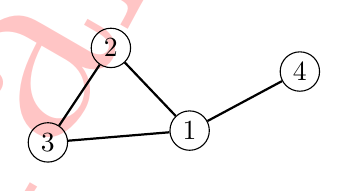
\begin{tikzpicture}[x=2.0cm,y=1.5cm]
            \tikzset{     
            e4c node/.style={circle,draw,minimum size=0.5cm,inner sep=0}, 
            e4c edge/.style={sloped,above,font=\footnotesize}
            }
            \node[e4c node] (1) at (0.9, 0.1) {1}; 
            \node[e4c node] (2) at (0.4, 0.8) {2}; 
            \node[e4c node] (3) at (0.0, 0.0) {3}; 
            \node[e4c node] (4) at (1.6, 0.6) {4}; 
            
            \path[-,draw,thick]
            (1) edge[e4c edge] (2)
            (1) edge[e4c edge] (3)
            (1) edge[e4c edge] (4)
            (2) edge[e4c edge] (3)
            ;
        \end{tikzpicture}
    \end{wrapfigure}
    W zbiorze wierzchołków grafu na rysunku obok istnieją dwa dwuelementowe niezależne podzbiory: $\{2, 4\}$ oraz $\{3, 4\}$.
    \bigskip

    Skojarzeniem $E_G$ jest na przykład $\big\{\{2, 3\}, \{1, 4\}\big\}$ i to skojarzenie jest doskonałe.
\end{example}

\textbf{Drzewo} to graf spójny bez cykli. Następujące warunki są równoważne:
\begin{enumerate}
    \item $G$ jest drzewem.
    \item Każde dwa wierzchołki w $G$ są połączone dokładnie jedną drogą.
    \item $G$ jest minimalny spójny.
    \item $G$ jest maksymalny acykliczny.
    \item $G$ jest spójny i $|V| = |E| + 1$.
\end{enumerate}

\subsection{Cykle Eulera i Hamiltona}
\textbf{Cykl Eulera} w grafie to cykl przechodzący przez każdą krawędź dokładnie raz. Powiemy, że graf jest \textbf{eulerowski}, gdy zawiera cykl Eulera.

Warunek konieczny i wystarczający: graf spójny $G$ jest eulerowski wtedy i tylko wtedy, gdy \purple{każdy jego wierzchołek jest parzystego stopnia}, a dla grafów skierowanych -- każdy wierzchołek ma równy stopień wyjściowy i wejściowy.
\bigskip

\textbf{Cykl Hamiltona} to cykl przechodzący przez każdy wierzchołek dokładnie raz. Powiemy, że graf jest \textbf{hamiltonowski}, gdy zawiera cykl Hamiltona.

W przeciwieństwie do cyklu Eulera, ogólny problem rozstrzygnięcia, czy dany graf ma cykl Hamiltona, jest zwykle bardzo trudny.

\begin{example}
    \begin{wrapfigure}{r}{8.3cm}
        \vspace{4mm}
        
        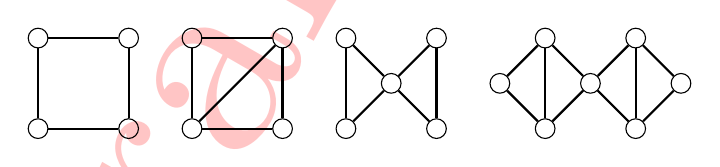
\begin{tikzpicture}[x=1.15cm,y=1.15cm]
            \tikzset{     
            e4c node/.style={circle,draw,minimum size=0.25cm,inner sep=0}, 
            e4c edge/.style={sloped,above,font=\footnotesize}
            }
            \node[e4c node] (1) at (0.0, 1.0) {}; 
            \node[e4c node] (2) at (0.0, 0.0) {}; 
            \node[e4c node] (3) at (1.0, 0.0) {}; 
            \node[e4c node] (4) at (1.0, 1.0) {}; 
            \node[e4c node] (1a) at (1.7, 1.0) {}; 
            \node[e4c node] (2a) at (1.7, 0.0) {}; 
            \node[e4c node] (3a) at (2.7, 0.0) {}; 
            \node[e4c node] (4a) at (2.7, 1.0) {};
            \node[e4c node] (1b) at (3.4, 1.0) {}; 
            \node[e4c node] (2b) at (3.4, 0.0) {}; 
            \node[e4c node] (3b) at (3.9, 0.5) {}; 
            \node[e4c node] (4b) at (4.4, 0.0) {};
            \node[e4c node] (5b) at (4.4, 1.0) {};
            \node[e4c node] (1c) at (5.1, 0.5) {}; 
            \node[e4c node] (2c) at (5.6, 1.0) {}; 
            \node[e4c node] (3c) at (5.6, 0.0) {}; 
            \node[e4c node] (4c) at (6.1, 0.5) {}; 
            \node[e4c node] (5c) at (6.6, 0.0) {};
            \node[e4c node] (6c) at (6.6, 1.0) {};
            \node[e4c node] (7c) at (7.1, 0.5) {}; 
            
            \path[-,draw,thick]
            (4) edge[e4c edge] (3)
            (3) edge[e4c edge] (2)
            (2) edge[e4c edge] (1)
            (1) edge[e4c edge] (4)
            (4a) edge[e4c edge] (3a)
            (3a) edge[e4c edge] (2a)
            (2a) edge[e4c edge] (1a)
            (1a) edge[e4c edge] (4a)
            (2a) edge[e4c edge] (4a)
            (1b) edge[e4c edge] (2b)
            (1b) edge[e4c edge] (3b)
            (2b) edge[e4c edge] (3b)
            (3b) edge[e4c edge] (4b)
            (3b) edge[e4c edge] (5b)
            (4b) edge[e4c edge] (5b)
            (1c) edge[e4c edge] (2c)
            (1c) edge[e4c edge] (3c)
            (2c) edge[e4c edge] (3c)
            (2c) edge[e4c edge] (4c)
            (3c) edge[e4c edge] (4c)
            (4c) edge[e4c edge] (5c)
            (4c) edge[e4c edge] (6c)
            (5c) edge[e4c edge] (6c)
            (5c) edge[e4c edge] (7c)
            (6c) edge[e4c edge] (7c)
            ;
        \end{tikzpicture}
    \end{wrapfigure}
    Na rysunku znajdują się kolejno przykłady grafu:
    \begin{itemize}
        \item eulerowskiego i hamiltonowskiego
        \item nieeulerowskiego, ale hamiltonowskiego
        \item eulerowskiego, ale niehamiltonowskiego
        \item nieeulerowskiego i niehamiltonowskiego
    \end{itemize}
\end{example}

\subsection{Grafy dwudzielne}

Graf $G$ jest grafem \textbf{dwudzielnym}, jeśli $V_G = V_1 \cup V_2$, gdzie $V_1$ i $V_2$ są rozłącznymi zbiorami wierzchołków i~każda krawędź ma jeden koniec w~$V_1$, a drugi w~$V_2$.

\textbf{Graf pełny dwudzielny} $K_{n, m}$ to taki, w którym $|V_1| = n, |V_2| = m$ oraz każdy wierzchołek z $V_1$ jest połączony z każdym innym z $V_2$.

Warunek konieczny i wystarczający: graf jest dwudzielny wtedy i tylko wtedy, gdy \purple{nie zawiera cykli nieparzystej długości}.
\bigskip

Skojarzenia (zbiory niezależnych krawędzi) w grafach dwudzielnych to \textbf{Systemy Różnych Reprezentantów} (SRR). Koncept ten jest wykorzystywany przy rozwiązywaniu niektórych problemów z teorii zbiorów, jak na poniższym przykładzie.

\begin{example}
    \begin{wrapfigure}{r}{5cm}
        \vspace{-4mm}
    
        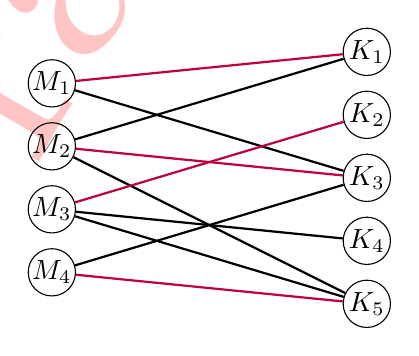
\begin{tikzpicture}[x=2cm,y=2cm]
            \tikzset{     
            e4c node/.style={circle,draw,minimum size=0.6cm,inner sep=0}, 
            e4c edge/.style={sloped,above,font=\footnotesize}
            }
            \node[e4c node] (M1) at (0.0, 1.4) {$M_1$}; 
            \node[e4c node] (M2) at (0.0, 1.0) {$M_2$}; 
            \node[e4c node] (M3) at (0.0, 0.6) {$M_3$}; 
            \node[e4c node] (M4) at (0.0, 0.2) {$M_4$}; 
            \node[e4c node] (K1) at (2.0, 1.6) {$K_1$}; 
            \node[e4c node] (K2) at (2.0, 1.2) {$K_2$}; 
            \node[e4c node] (K3) at (2.0, 0.8) {$K_3$}; 
            \node[e4c node] (K4) at (2.0, 0.4) {$K_4$}; 
            \node[e4c node] (K5) at (2.0, 0.0) {$K_5$}; 
            
            \path[-,draw,thick]
            (M1) edge[e4c edge, purple] (K1)
            (M1) edge[e4c edge] (K3)
            (M2) edge[e4c edge] (K1)
            (M2) edge[e4c edge, purple] (K3)
            (M2) edge[e4c edge] (K5)
            (M3) edge[e4c edge, purple] (K2)
            (M3) edge[e4c edge] (K4)
            (M3) edge[e4c edge] (K5)
            (M4) edge[e4c edge] (K3)
            (M4) edge[e4c edge, purple] (K5)
            ;
        \end{tikzpicture}
    \end{wrapfigure}

    Chcemy wybrać żony dla mężczyzn $M_1, ..., M_4$ wśród kandydatek $K_1, ..., K_5$, tak aby każdy mężczyzna ożenił się z kobietą, którą zna. 
    \bigskip
    
    Sporządźmy (dwudzielny) graf znajomości: jeśli $M_i$ zna $K_j$, to odpowiednie wierzchołki połączymy krawędzią.
    \bigskip

    Rozwiązaniem problemu jest wybór Systemu Różnych Reprezentantów, na przykład odpowiadającego skojarzeniu $$\big\{\{M_1, K_1\}, \{M_2, K_3\}, \{M_3, K_2\}, \{M_4, K_5\}\big\}$$
\end{example}

Naturalnie nasuwającym się pytaniem jest to, kiedy System Różnych Reprezentantów dla danego grafu dwudzielnego w ogóle istnieje. Odpowiedź przynosi nam \textbf{twierdzenie Halla}. Okazuje się, że warunkiem koniecznym i wystarczającym na istnienie SRR jest to, by \purple{każda podgrupa $k$ kobiet znała co najmniej $k$ mężczyzn}.

\subsection{Planarność}

\textbf{Płaskie włożenie} grafu w płaszczyznę to przedstawienie go graficznie w postaci, w której jego krawędzie nie przecinają się. Graf, który ma takie włożenie, nazywamy \textbf{planarnym}.

\textbf{Ścianą} w płaskim włożeniu nazywać będziemy maksymalny spójny obszar płaszczyzny rozłączny z grafem. Jedna ze ścian (zewnętrzna) jest nieograniczona.

\begin{example}
    Poniżej przedstawiono klikę $K_4$ i jej płaską reprezentację, wraz z wyróżnionymi ścianami. Płaskie włożenie uzyskano, przesuwając wierzchołek z lewego górnego rogu zgodnie ze strzałką.
    \begin{center}
        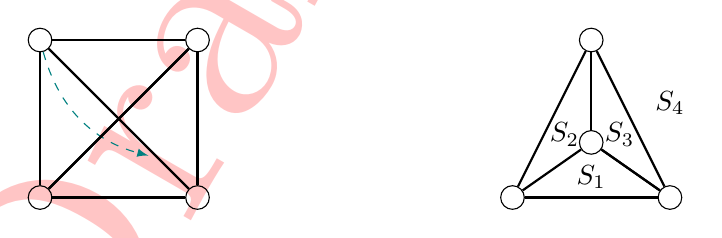
\begin{tikzpicture}[x=2cm,y=2cm]
            \tikzset{     
            e4c node/.style={circle,draw,minimum size=0.3cm,inner sep=0}, 
            e4c edge/.style={sloped,above,font=\footnotesize}
            }
            \node[e4c node] (1) at (0.0, 1.0) {}; 
            \node[e4c node] (2) at (0.0, 0.0) {}; 
            \node[e4c node] (3) at (1.0, 0.0) {}; 
            \node[e4c node] (4) at (1.0, 1.0) {}; 
            \node[e4c node] (1a) at (3.0, 0.0) {}; 
            \node[e4c node] (2a) at (4.0, 0.0) {}; 
            \node[e4c node] (3a) at (3.5, 1.0) {}; 
            \node[e4c node] (4a) at (3.5, 0.35) {};
            \node[] (M) at (0.75, 0.25) {};
            \node[] (S1) at (3.5, 0.13) {$S_1$};
            \node[] (S2) at (3.33, 0.4) {$S_2$};
            \node[] (S3) at (3.68, 0.4) {$S_3$};
            \node[] (S4) at (4.0, 0.6) {$S_4$};

            \path[-latex, bend right = 30, teal, dashed]
            (1) edge[] (M);
            
            \path[-,draw,thick]
            (1) edge[e4c edge] (2)
            (2) edge[e4c edge] (3)
            (3) edge[e4c edge] (4)
            (4) edge[e4c edge] (1)
            (1) edge[e4c edge] (3)
            (2) edge[e4c edge] (4)
            (2) edge[e4c edge] (4)
            (1a) edge[e4c edge] (2a)
            (2a) edge[e4c edge] (3a)
            (3a) edge[e4c edge] (4a)
            (4a) edge[e4c edge] (1a)
            (1a) edge[e4c edge] (3a)
            (2a) edge[e4c edge] (4a)
            (2a) edge[e4c edge] (4a)
            ;
        \end{tikzpicture}
    \end{center}
\end{example}

Liczba ścian płaskiego włożenia grafu spełnia \textbf{wzór Eulera}:
$$\purple{v - e + f = 2,}$$
gdzie $v$ -- liczba wierzchołków, $e$ -- liczba krawędzi, $f$ -- liczba ścian. Ze wzoru Eulera otrzymujemy górne oszacowanie liczby krawędzi w grafie planarnym:
$$\text{dla } v \geq 3 \text{ zachodzi } \purple{e \leq 3v - 6},$$
z którego wynika, że na przykład graf $K_5$ jest nieplanarny.

Dla grafów niezawierających trójkątów (cykli długości 3) prawdziwa jest jeszcze mocniejsza teza:
$$\purple{e \leq 2v - 4},$$
z której wiadomo, że graf dwudzielny $K_{3, 3}$ także jest nieplanarny. Z powyższych wzorów można też wywnioskować, że \purple{każdy graf planarny zawiera wierzchołek stopnia $\leq 5$}, co stanowi warunek konieczny planarności.
\bigskip

Grafy $G$ i $H$ nazwiemy \textbf{homeomorficznymi}, jeśli można je uczynić izomorficznymi poprzez dostawianie wierzchołków na ich krawędziach. Dla przykładu, poniższe dwa grafy są homeomorficzne.
\begin{center}
    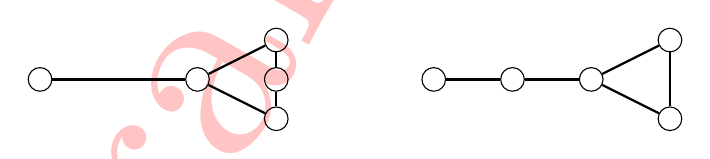
\begin{tikzpicture}[x=1cm,y=1cm]
        \tikzset{     
        e4c node/.style={circle,draw,minimum size=0.3cm,inner sep=0}, 
        e4c edge/.style={sloped,above,font=\footnotesize}
        }
        \node[e4c node] (1) at (0.0, 0.5) {}; 
        \node[e4c node] (2) at (2.0, 0.5) {}; 
        \node[e4c node] (3) at (3.0, 1.0) {}; 
        \node[e4c node] (4) at (3.0, 0.5) {}; 
        \node[e4c node] (5) at (3.0, 0.0) {}; 
        \node[e4c node] (1a) at (5.0, 0.5) {}; 
        \node[e4c node] (2a) at (6.0, 0.5) {}; 
        \node[e4c node] (3a) at (7.0, 0.5) {}; 
        \node[e4c node] (4a) at (8.0, 1.0) {}; 
        \node[e4c node] (5a) at (8.0, 0.0) {}; 
        
        \path[-,draw,thick]
        (1) edge[e4c edge] (2)
        (2) edge[e4c edge] (3)
        (3) edge[e4c edge] (4)
        (4) edge[e4c edge] (5)
        (5) edge[e4c edge] (2)
        (1a) edge[e4c edge] (2a)
        (2a) edge[e4c edge] (3a)
        (3a) edge[e4c edge] (4a)
        (4a) edge[e4c edge] (5a)
        (5a) edge[e4c edge] (3a)
        ;
    \end{tikzpicture}
\end{center}

Warunek konieczny i wystarczający istnienia płaskiego włożenia grafu opisuje \textbf{twierdzenie Kuratowskiego}: graf jest nieplanarny wtedy i tylko wtedy, gdy \purple{zawiera podgraf homeomorficzny z $K_5$ lub $K_{3,3}$}.

\begin{exam}
    Dany jest graf $G$ o $n \leq 6$ wierzchołkach i $m$ krawędziach. Wówczas
    \answers{$G$ lub dopełnienie $G$ jest planarne}{jeśli $m < 10$, to $G$ jest planarny}{jeśli $m > 10$, to $G$ nie jest planarny}
    \bigskip

    Rozwiążemy podpunkt \textbf{A.} Dla $n \leq 4$ jasne jest, że $G$ jest planarny (twierdzenie Kuratowskiego). Dla $n = 5$ jedynym istniejącym grafem nieplanarnym $G$ jest $K_5$, ale wtedy dopełnienie $G$ jest planarne. Rozpatrzmy $n = 6$ i załóżmy, że $G$ jest nieplanarny. Z twierdzenia Kuratowskiego wynika, że $G$ zawiera podgraf homeomorficzny z $K_5$ lub $K_{3, 3}$.
    
    Podgraf homeomorficzny z $K_5$ ma 5 wierzchołków stopnia 4. Jeśli podgrafem homeomorficznym w $G$ jest $K_5$, to dopełnienie $G$ ma przynajmniej 5 wierzchołków stopnia $< 2$, więc na podstawie twierdzenia Kuratowskiego dopełnienie $G$ jest planarne.

    Z drugiej strony, jeśli $G$ zawierałoby podgraf homeomorficzny z $K_{3,3}$, to skoro $G$ ma 6 wierzchołków, musi być $G = K_{3,3}$ i wtedy dopełnienie $G$ jest planarne. Podpunkt \textbf{A.} jest więc prawdziwy.
    \bigskip

    Do pozostałych podpunktów nietrudno znaleźć kontrprzykłady: dla podpunktu \textbf{B.} wystarczy wziąć $G = K_{3,3}$, a dla podpunktu \textbf{C.} graf z rysunku poniżej ($n = 6, m = 11$). Oba te stwierdzenia są więc fałszywe.
    
    \begin{center}
    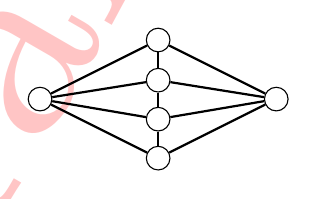
\begin{tikzpicture}[x=1.5cm,y=1.5cm]
        \tikzset{     
        e4c node/.style={circle,draw,minimum size=0.3cm,inner sep=0}, 
        e4c edge/.style={sloped,above,font=\footnotesize}
        }
        \node[e4c node] (1) at (0.0, 0.5) {}; 
        \node[e4c node] (2) at (1.0, 1.0) {}; 
        \node[e4c node] (3) at (1.0, 0.66) {}; 
        \node[e4c node] (4) at (1.0, 0.33) {}; 
        \node[e4c node] (5) at (1.0, 0.0) {};
        \node[e4c node] (6) at (2.0, 0.5) {};
        
        \path[-,draw,thick]
        (1) edge[e4c edge] (2)
        (1) edge[e4c edge] (3)
        (1) edge[e4c edge] (4)
        (1) edge[e4c edge] (5)
        (2) edge[e4c edge] (3)
        (3) edge[e4c edge] (4)
        (4) edge[e4c edge] (5)
        (6) edge[e4c edge] (2)
        (6) edge[e4c edge] (3)
        (6) edge[e4c edge] (4)
        (6) edge[e4c edge] (5)
        ;
    \end{tikzpicture}
    \end{center}
\end{exam}

\subsection{Kolorowanie grafów}

\textbf{Kolorowanie grafu} $G$ za pomocą $k$ kolorów to funkcja $f : V_G \to \{1, ..., k\}$ przyporządkowująca kolory wierzchołkom w taki sposób, że każde dwa wierzchołki połączone krawędzią są w różnych barwach.

Najmniejsze $k$, dla którego istnieje $k$-kolorowanie $G$, nazywamy \textbf{liczbą chromatyczną} $\chi(G)$. Znalezienie jej jest w ogólnym przypadku trudne. 
\bigskip

Istnieje szereg twierdzeń pomagających znaleźć liczbę chromatyczną. Jednym z nich jest \textbf{twierdzenie o czterech barwach}:
$$\purple{\text{jeśli graf jest planarny, to } \chi(G) \leq 4}.$$

Ponadto, z prostej obserwacji wynika, że
$$\purple{\chi(G) = 2 \wtw G \text{ jest dwudzielny}}.$$

Łącząc powyższe informacje, otrzymujemy wniosek, że graf planarny niebędący grafem dwudzielnym jest zawsze albo 3-, albo 4-kolorowalny. Okazuje się jednak, że sprawdzenie tej informacji dla danego grafu jest problemem NP-trudnym.
\bigskip

\begin{wrapfigure}{r}{2cm}
    \vspace{-5mm}
    
    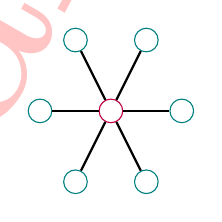
\begin{tikzpicture}[x=1.8cm,y=1.8cm]
        \tikzset{     
        e4c node/.style={circle,draw,minimum size=0.3cm,inner sep=0}, 
        e4c edge/.style={sloped,above,font=\footnotesize}
        }
        \node[e4c node, purple] (S) at (0.5, 0.5) {};
        \node[e4c node, teal] (1) at (0.25, 1.0) {}; 
        \node[e4c node, teal] (2) at (0.75, 1.0) {}; 
        \node[e4c node, teal] (3) at (1.0, 0.5) {}; 
        \node[e4c node, teal] (4) at (0.75, 0.0) {};
        \node[e4c node, teal] (5) at (0.25, 0.0) {};
        \node[e4c node, teal] (6) at (0.0, 0.5) {};
        
        \path[-,draw,thick]
        (S) edge[e4c edge] (1)
        (S) edge[e4c edge] (2)
        (S) edge[e4c edge] (3)
        (S) edge[e4c edge] (4)
        (S) edge[e4c edge] (5)
        (S) edge[e4c edge] (6)
        ;
    \end{tikzpicture}
\end{wrapfigure}

Innym narzędziem pozwalającym ograniczyć liczbę chromatyczną z góry jest \textbf{twierdzenie Brooksa}. Oznaczmy jako $\Delta(G)$ maksymalny stopień wierzchołka w grafie $G$. Jeśli spójny graf $G$ nie jest cyklem nieparzystej długości ani kliką, to $\purple{\chi(G) \leq \Delta(G)}$.

Ale uwaga: to oszacowanie może być bardzo niedokładne, na przykład gwiazda (rysunek obok) ma $\chi(G) = 2$ i dowolnie duże $\Delta(G)$ (wystarczy dokładać wierzchołki na brzegu i łączyć je z środkowym).
\bigskip

Wyróżniamy także \textbf{kolorowanie krawędziowe}, czyli funkcję $f : E_G \to \{1, ..., k\}$, taką że incydentne krawędzie są różnego koloru. Analogicznie, \textbf{indeks chromatyczny} $\chi_e(G)$ to najmniejsze $k$, dla którego istnieje $k$-kolorowanie krawędziowe.

Po krótkim rozumowaniu łatwo znaleźć dolne oszacowanie indeksu chromatycznego: $\chi_e(G) \geq \Delta(G)$, jednakże o dodatkowym, nieoczywistym fakcie mówi \textbf{twierdzenie Vizinga}: $$\chi_e(G) \leq \Delta(G) + 1.$$

W związku z tym \purple{indeks chromatyczny $\chi_e(G)$ jest zawsze równy albo $\Delta(G)$, albo $\Delta(G) + 1$} (dla dowolnego $G$). Mimo to rozstrzygnięcie, który wariant jest prawdziwy dla danego grafu, jest w ogólnym przypadku trudne. Jeśli jednak graf $G$ jest dwudzielny, to $\chi_e(G) = \Delta(G)$.

\begin{problems}
    \prob Graf $G$ ma cykl Eulera, ale nie ma cyklu Hamiltona. Wynika z tego, że
    \answers{dopełnienie grafu $G$ ma cykl Hamiltona}{$G$ ma ścieżkę Hamiltona}{$G$ ma więcej niż jedną dwuspójną składową}

    \prob Każdy graf nieplanarny o $n$ wierzchołkach
    \answers{zawiera podgraf $K_{3,3}$ lub $K_5$}{ma co najmniej $3n-5$ krawędzi}{ma liczbę chromatyczną nie mniejszą niż 5}

    \prob Graf $100$-wierzchołkowy $G$ ma liczbę chromatyczną $3$. Wynika z tego, że graf $G$
    \answers{jest planarny}{zawiera cykl}{zawiera niezależny zbiór wierzchołków rozmiaru $34$}

    \prob Dany jest $k$-regularny graf o $n$ wierzchołkach i $m$ krawędziach. Wtedy
    \answers
    {$k$ jest parzyste lub $n$ jest parzyste}
    {$k$ jest dzielnikiem $n$}
    {$k$ jest dzielnikiem $m$}

    \prob $G$ jest grafem spójnym o $n > 2$ wierzchołkach i takim, że każda jego krawędź należy do pewnego cyklu prostego. Wynika z tego, że
    \answers
    {$G$ ma cykl Hamiltona}
    {graf otrzymany przez usunięcie z $G$ jednego wierzchołka jest spójny}
    {każde dwa różne wierzchołki w $G$ są połączone przynajmniej dwiema krawędziowo rozłącznymi ścieżkami}

    \prob Graf $G$ ma $n > 2$ wierzchołków i $n$ krawędzi. Wynika z tego, że graf $G$
    \answers
    {jest spójny}
    {zawiera cykl}
    {jest planarny}

    \prob $G$ jest $n$-wierzchołkowym grafem spójnym regularnym stopnia 3. Wynika z tego, że
    \answers{$n$ jest parzyste}{$G$ jest planarny}{liczba chromatyczna $\chi(G) \leq 4$}
\end{problems}

% Grześ
\section{Teoria liczb}

Na wstępie, przypomnijmy sobie podstawowe definicje i notacje związane z podzielnością liczb.
\begin{itemize}
    \item Dla $b>0$ i dowolnego $a$ istnieją jednoznacznie wyznaczone $q$ (\textbf{iloraz}) i $0\leq r<b$ (\textbf{reszta}) takie, że $a=b\cdot q + r$.

    \item \textbf{Największy wspólny dzielnik} (NWD) liczb $a,b$ to liczba $s$ taka, że $s\mid a,b$ oraz jeśli $d\mid a,b$, to także $d\mid s$. $\mathrm{NWD}(a,b)$ to najmniejszy dodatni element zbioru $\{ax+by : x,y\in\ZZ\}$.
    
    \item Jeśli $\mathrm{NWD}(a,b)$ jest równe 1, to $a$ i $b$ są \textbf{względnie pierwsze} ($a\perp b$).

    \item Znane jest \textbf{podstawowe twierdzenie arytmetyki}: każda liczba $a>0$ ma rozkład $a=\prod_{i=1}^{n}p_i$, gdzie $p_i$ to \textbf{czynniki pierwsze}, który jest jednoznaczny z dokładnością do kolejności elementów.
\end{itemize}







\begin{example}
    Niech $a=p_1^{\alpha_1}p_2^{\alpha_2}\cdots p_k^{\alpha_k}$ oraz $b=p_1^{\beta_1}p_2^{\beta_2}\cdots p_k^{\beta_k}$, gdzie $p_i$ to różne czynniki pierwsze. Wtedy
    \begin{itemize}
        \item $b\mid a \wtw \forall_i \ \beta_i\leq\alpha_i$
        \item $b\perp a \wtw \forall_i \ \min(\alpha_i,\beta_i)=0$
        \item $\mathrm{NWD}(a,b)=\prod_{i=1}^k p_i^{\min(\alpha_i,\beta_i)}$
        \item $\purple{\mathrm{NWW}(a,b)=\frac{ab}{\mathrm{NWD}(a,b)}}=\prod_{i=1}^k p_i^{\max(\alpha_i,\beta_i)}$
    \end{itemize}
\end{example}

\begin{exam}
    Dla dowolnych dodatnich liczb całkowitych $a$ i $b$ zachodzi implikacja
    \answers{$a^2 \ | \ b^2 \Rightarrow a^3 \ | \ b^3$}{$a^2 \ | \ b^3 \Rightarrow a \ | \  b$}{$a^3 \ | \  b^2 \Rightarrow a \ | \  b$}
    \begin{enumerate}[\bf A.]
        \item Skoro $a^2$ dzieli $b^2$, to możemy zapisać, że $b^2=ka^2$ dla pewnego $k\in\ZZ$. Stąd $k=\frac{b^2}{a^2}=(\frac{b}{a})^2$. Widzimy, że $a$ musi być dzielnikiem $b$, ponieważ $k$ ma być całkowite. Skoro $a\mid b$, to również $a^3\mid b^3$, więc odpowiedź to \texttt{TAK}.
        \item Weźmy $a=2^3$ i~$b=2^2$. Oczywiście $a^2=2^6=b^3$, więc $a^2\mid b^3$, ale $a\nmid b$, więc odpowiedź to \texttt{NIE}.
        \item Podobnie jak w podpunkcie \textbf{A.}, zapiszmy daną relację jako $b^2=ka^3$ dla pewnego $k\in\ZZ$. Stąd $ak=(\frac{b}{a})^2$. Skoro $ak$ jest liczbą całkowitą (jako iloczyn liczb całkowitych), to $\frac{b}{a}$ również musi być całkowite, więc $a\mid b$ i odpowiedzią jest \texttt{TAK}.
    \end{enumerate}
\end{exam}

\subsection{Algorytm Euklidesa}

Algorytm Euklidesa pozwala efektywnie wyznaczyć $\mathrm{NWD}(a,b)$ oraz $x,y$ takie, że $\mathrm{NWD}(a,b)=ax+by$:
\begin{itemize}
    \item jeśli $b=0$, to $\langle x,y\rangle\leftarrow\langle1,0\rangle$
    \item wpp. mamy $x',y'$ takie, że $\mathrm{NWD}(a,b)=\mathrm{NWD}(b,a\mod{b})=bx'+(a\mod{b})y'$, ale $a\mod{b}=a-b\cdot\left\lfloor\frac{a}{b}\right\rfloor$, więc można przyjąć $\langle x,y\rangle\leftarrow\langle y',x'-y'\cdot\left\lfloor\frac{a}{b}\right\rfloor\rangle$
\end{itemize}

\begin{example}
    Znajdziemy $x,y$, dla których $\mathrm{NWD}(36,15)=36x+15y$:
    $$
    \begin{matrix}
        a & b & & x & y \\
        36 & 15 & \downarrow\ \uparrow & \purple{-2} & \purple{5} \\
        15 & 6 & \downarrow\ \uparrow & 1 & -2 \\
        6 & 3 & \downarrow\ \uparrow & 0 & 1 \\
        3 & 0 & \rightarrow & 1 & 0
    \end{matrix}
    $$
    Na początku stosujemy wzór $\mathrm{NWD}(a,b)=\mathrm{NWD}(b,a\mod{b})$ tak długo, dopóki nie otrzymamy 0 w drugiej kolumnie. Następnie korzystamy z pierwszego przypadku i przypisujemy wartości $\langle x,y\rangle\leftarrow\langle1,0\rangle$. Idąc do góry, stosujemy wzór $\langle x,y\rangle\leftarrow\langle y',x'-y'\cdot\left\lfloor\frac{a}{b}\right\rfloor\rangle$. Ostatecznie otrzymujemy
    $$\mathrm{NWD}(36,15)=36\cdot\purple{(-2)}+15\cdot\purple{5}=3$$
\end{example}

\subsection{Kongruencje}

Dla $n>0$ mówimy, że \textbf{$a$ przystaje do $b$ modulo $n$} ($a\equiv b\mod{n}$), gdy $n\mid a-b$, czyli $a$ i $b$ dają tę samą resztę z dzielenia przez $n$.

Własności kongruencji:
\begin{itemize}
    \item $\equiv$ (mod $n$) jest relacją równoważności, jako zbiór reprezentantów jej klas abstrakcji można wziąć $Z_n=\{0,\ldots,n-1\}$
    \item kongruencje można dodawać, odejmować, mnożyć i potęgować stronami (jak równania)
    \item kongruencję $a\equiv b$ (mod $n$) można podzielić obustronnie przez $d$ tylko, gdy $d\perp n$
    \item $ad\equiv bd\mod{nd}\wtw a\equiv b\mod{n}$
\end{itemize}
\bigskip

Jeśli $n_1\perp n_2$, to układ dwóch kongruencji
$$
\begin{cases}
    a \equiv b \mod{n_1} \\
    a \equiv b \mod{n_2}
\end{cases}
$$
jest równoważny pojedynczej kongruencji $a\equiv b\mod{n_1n_2}$. Na tym prostym spostrzeżeniu bazuje dużo silniejsze \textbf{chińskie twierdzenie o resztach}:

Niech $n=n_1\cdots n_k$, gdzie $n_i$ parami względnie pierwsze. Wtedy dla dowolnych $a_1,\ldots,a_k$ istnieje dokładnie jedno $a\in\{0,\ldots,n-1\}$ takie, że
$$a \equiv a_i \mod{n_i}, \text{ dla } i\in\{1,\ldots,k\}$$

\begin{example}
    Niech $\langle n_1,n_2,n_3\rangle = \langle7,11,13\rangle$ i wtedy $n=1001$. Weźmy $\langle a_1,a_2,a_3\rangle = \langle5,3,11\rangle$ i znajdźmy $a$ takie, że $a$ daje resztę $a_i \mod{n_i}$ dla $i=1,2,3$.

    Znajdujemy $m_i$ takie, że $n_j\mid m_i$ dla $j\neq i$ oraz $m_i\perp n_i$ (na przykład $m_i=\frac{n}{n_i}$) i przyjmujemy
    $$a=\sum_i(a_im_i(m_i^{-1}\mod{n_i}))\mod{n},$$
    gdzie $m^{-1}\mod{n}$ to odwrotność modularna, czyli takie $x$, że $mx\equiv1\mod{n}$. Odwrotność modularną łatwo znaleźć za pomocą algorytmu Euklidesa jako współczynnik przy $m_i$ w wyrażeniu $m_ix+n_iy=\mathrm{NWD}(m_i,n_i)=1$. U nas
    $$a=(5\cdot143\cdot5+3\cdot91\cdot4+11\cdot77\cdot12)\mod{1001}=817$$
\end{example}

Inne, często wykorzystywane przy kongruencjach twierdzenie to \textbf{małe twierdzenie Fermata}: jeśli $p$ jest liczbą pierwszą i $p\nmid a$, to $\purple{a^{p-1}\equiv1\mod{p}}$.

\subsection{Funkcja Eulera}

Niech $Z_n^*=\{1\leq k\leq n : k\perp n\}$, czyli zbiór liczb całkowitych dodatnich niewiększych niż $n$ i względnie pierwszych z $n$. \textbf{Funkcja Eulera} $\Phi:\NN\to\NN$ jest określona jako $\Phi(n)=|Z_n^*|$, czyli liczba liczb mniejszych od $n$ względnie pierwszych z $n$.

Własności:
\begin{itemize}
    \item jeśli $p$ jest pierwsza, to $\Phi(p^k)=p^k-p^{k-1}$
    \item multiplikatywność: jeśli $m\perp n$, to $\Phi(mn)=\Phi(m)\Phi(n)$
    \item wzór iloczynowy: $\Phi(n)=n\prod_{p\mid n}(1-\frac{1}{p})$, gdzie $p$ jest pierwsza
\end{itemize}

Funkcja Eulera pozwala nam uogólnić małe twierdzenie Fermata -- w ten sposób powstało \textbf{twierdzenie Eulera}: jeśli $a\perp n$, to $\purple{a^{\Phi(n)}\equiv1\mod{n}}$.

\begin{example}
    Obliczymy $2^{65536}$ mod 2009 za pomocą twierdzenia Eulera. Mamy $2009 = 7^2\cdot41$, więc korzystając z własności funkcji Eulera:
    $$\Phi(2009)=\Phi(7^2)\Phi(41)=42\cdot40=1680$$
    Stąd dostajemy
    $$2^{1680}\equiv1\mod{2009}$$
    Znajdziemy teraz iloraz i resztę z dzielenia 65536 przez 1680:
    $$65536=1680\cdot q+r=1680\cdot39+16$$
    To pozwoli nam dojść do szukanego wyrażenia -- podnosimy kongruencję stronami do potęgi $q=39$, a następnie przemnażamy stronami przez $2^r=2^{16}$:
    $$2^{1680\cdot39+16}\equiv2^{16}\mod{2009}$$
    stąd
    $$2^{65536}\equiv65536\equiv1248\mod{2009}$$
    Trzeba jednak pamiętać, że twierdzenia Eulera możemy używać jedynie, gdy $a\perp n$. W naszym przypadku $n=7^2\cdot41$, więc oczywiście jest względnie pierwsze z $a=2$.
\end{example}

\begin{problems}
    \prob Liczba $p > 2$ jest pierwsza. Wynika z tego, że
    \answers{$(p-2)^{p-1}-1$ dzieli się przez $p$}{$(p-2)^{p^2-1}-1$ dzieli się przez $p^2$}{$(p-2)^{p^3-p^2}-1$ dzieli się przez $p^3$}

    \prob Jeśli $a, b$ są dodatnimi liczbami całkowitymi, to $\mathrm{NWD}(a,b)$ jest najmniejszym dodatnim elementem zbioru
    \answers{$\{ax + by \mid x, y \in \mathbb{Z}\}$}{$\{a(x+y) + b(x-y) \mid x, y \in \mathbb{Z}\}$}{$\{2ax + 3by \mid x,y \in \mathbb{Z}\}$}

    \prob Dane są dodatnie liczby całkowite $a, b$, których największy wspólny dzielnik jest równy $d$. Wówczas względnie pierwsze są liczby
    \answers{$\frac{a}{d}$ oraz $b$}{$\frac{ab}{d^2}$ oraz $b$}{$\frac{a^2}{d^2}$ oraz $\frac{b^2}{d^2}$}
\end{problems}

% Błażej
\section{Asymptotyka}

\textbf{Notacja asymptotyczna} pozwala ukryć zbędne nadmiarowe informacje, uprościć operowanie wyrażeniami i~ocenić przybliżone graniczne zachowanie.

Jeśli $f, g : \NN \to \RR^+$, to zapisujemy $\purple{f = O(g)}$, gdy dla pewnej stałej $c$ i dostatecznie dużych $n$ zachodzi
$$f(n) \leq c \cdot g(n)$$

Zapis $f = O(g)$ czytamy jako ,,$f$ \textbf{jest co najwyżej rzędu} $g$'' albo ,,$f$ rośnie co najwyżej tak szybko, jak $g$''.

Inne stosowane oznaczenia:
\begin{itemize}
    \item $\purple{f = \Omega(g)} \wtw g = O(f)$ \hfill ,,$f$ rośnie co najmniej tak szybko, jak $g$"
    \item $\purple{f = \Theta(g)} \wtw f = O(g) \land g = O(f)$ \hfill ,,$f$ rośnie tak samo szybko, jak $g$"
    \item $\purple{f = o(g)} \wtw \Limn \frac{f(n)}{g(n)} = 0$ \hfill ,,$f$ rośnie istotnie wolniej niż $g$"
    \item $\purple{f = \omega(g)} \wtw g = o(f) \wtw \Limn \frac{f(n)}{g(n)} = \infty$ \hfill ,,$f$ rośnie istotnie szybciej niż $g$"
    \item $\purple{f \sim g} \wtw \Limn \frac{f(n)}{g(n)} = 1$ \hfill ,,$f$ jest asymptotycznie równe $g$"
\end{itemize}

Definicja notacji asymptotycznej jest ściśle powiązana z definicją granicy. Istotnie, jeśli wartość $\Limn \frac{f(n)}{g(n)}$ jest określona, możemy z niej wywnioskować relację asymptotyczną między $f$ i $g$:
$$\Limn \frac{f(n)}{g(n)} \neq \infty \ \Rightarrow \ f = O(g), \qquad \Limn \frac{f(n)}{g(n)} \neq 0 \ \Rightarrow \ f = \Omega(g),$$
$$\Limn \frac{f(n)}{g(n)} \neq 0, \infty \ \Rightarrow \ f = \Theta(g)$$

Powszechnie znane są także zależności asymptotyczne między charakterystycznymi funkcjami. Oznaczmy $f < g$, jeśli $f = o(g)$. Wtedy dla dowolnych $a \in (0, 1)$ i $b > 1$ zachodzi:
$$\purple{\frac{1}{b^n} < \frac{1}{n^b} < 1 < (\log \log n)^b < \log n < n^a < n < n \log n < n^b < b^n < n!}$$

\subsection{Twierdzenie o rekurencji uniwersalnej}

Równania rekurencyjne typu ,,\textbf{dziel i zwyciężaj}'' są postaci
$$\purple{T(n) = a \cdot T\left(\floor{\frac{n}{b}}\right) + f(n)},$$
gdzie $f$ jest funkcją nieujemną oraz $a, b \in \RR^+$. Tak zdefiniowana funkcja $T$ stanowi pewien schemat działania algorytmów typu ,,dziel i zwyciężaj'' -- problem o rozmiarze $n$ dzielony jest na $a$ podproblemów, każdy wielkości $\floor{\frac{n}{b}}$, funkcja $f$ przedstawia koszt dzielenia problemu oraz połączenia rozwiązań podproblemów.

W ogólnej postaci powyższego równania można \textbf{zignorować podłogi i sufity} (łatwo pokazać, że asymptotycznie nie zmieni to rozwiązania).

Takie równania łatwo rozwiązujemy, korzystając z \textbf{twierdzenia o rekurencji uniwersalnej}:
\begin{itemize}
    \item jeśli $f(n) = O(n^{\log_b a - \epsilon})$ dla pewnej stałej $\epsilon > 0$, to $\purple{T(n) = \Theta(n^{\log_b a})}$
    \item jeśli $f(n) = \Theta(n^{\log_b a})$, to $\purple{T(n) = \Theta(n^{\log_b a} \log n)}$
    \item jeśli $f(n) = \Omega(n^{\log_b a + \epsilon})$ dla pewnej stałej $\epsilon > 0$ i jeżeli $a \cdot f(\frac{n}{b}) \leq c \cdot f(n)$ dla pewnej stałej $c \in (0, 1)$ i~dostatecznie dużych $n$, to $\purple{T(n) = \Theta(f(n))}$
\end{itemize}

Intuicyjnie, każdy z trzech przypadków rekurencji uniwersalnej sprowadza się do stwierdzenia, która z funkcji $n^{\log_b a}$ i $f$ jest ,,większa''. Gdy znana jest odpowiedź na to pytanie, automatycznie znane jest asymptotyczne ograniczenie danej rekursji -- jest nią owa ,,większa'' funkcja.

\begin{example}
    Koszt rozwiązania algorytmu wyszukiwania binarnego opisuje równanie
    $$T(n) = T\left(\frac{n}{2}\right) + O(1).$$
    Korzystając z twierdzenia o rekurencji uniwersalnej, odczytujemy $a = 1, b = 2$ i wtedy $f(n) = \Theta(n^{\log_2 1}) = \Theta(1)$. Stąd otrzymujemy rozwiązanie $T(n) = O(\log n)$.
\end{example}

\begin{problems}
    \prob Funkcje $f, g: \NN \rightarrow \RR$ przyjmują wyłącznie wartości dodatnie i są niemalejące. Wynika z tego, że
    \answers{jeśli $f = O(g)$ i $g = O(f)$, to istnieje skończona granica $\Limn \frac{f(n)}{g(n)}$}{jeśli $f = O(g)$, to $f/g = O(1)$}{$f = O(g)$ lub $g = O(f)$}

    \prob Rozwiązaniem równania rekurencyjnego $T(n)=2T(\lfloor n/2 \rfloor)+f(n)$ dla $n>1$, $T(1)=0$, jest
    \answers{$T(n)=\Theta(\log{n})$, jeśli $f(n)=O(1)$}{$T(n)=\Theta(n)$, jeśli $f(n)=\Theta(\sqrt{n})$}{$T(n)=\Theta(n^2)$, jeśli $f(n)=\Theta(n^2)$}
\end{problems}

\begin{solutions}
    % Jasiek
    \sol Niech $f$ oznacza permutację $\lr{3, 6, 1, 4, 2, 5}$ i niech $f^k$ oznacza $k$-krotne złożenie permutacji $f$. Wynika z tego, że
    \answerss{$f^8 = \lr{1, 2, 3, 4, 5, 6}$}{$f^7=f$}{$f^4=f^{16}$}{NIE}{TAK}{TAK}

    Rozważmy zapis cyklowy danej permutacji: $[1, 3][2, 6, 5][4]$. Rozmiary tych cykli to kolejno 2, 3, 1. To oznacza, że $f^6 = id$, gdzie $id$ to permutacja identycznościowa. Z tego powodu dla dowolnego $k$ mamy $f^k = f^{k + 6}$ i po odpowiednim podstawieniu łatwo uzyskujemy odpowiedzi do zadania.

    % Kasia
    \sol Jeśli ponumerujemy permutacje zbioru $\{1, 2, 3, 4, 5\}$ od $1$ do $120$ w porządku leksykograficznym, to permutacją o numerze $60$ będzie
    \answerss
    {$\lr{3, 5, 1, 2, 4}$}
    {$\lr{3, 4, 1, 2, 5}$}
    {$\lr{3, 2, 5, 4, 1}$}
    {NIE}{NIE}{TAK}
    Jak łatwo zauważyć, permutacji z określoną liczbą na pierwszym miejscu jest dokładnie $4!=24$. Możemy zatem określić, że permutacje z numerami 1-24 mają jako pierwszą liczbę ,,1'', numery 25-48 -- liczbę ,,2'', a numery 49-72 -- liczbę ,,3''. Wiemy również, że permutacji z określonymi liczbami na pierwszych dwóch miejscach jest dokładnie $3!=6$. Zatem możemy określić, że permutacje z numerami 49-54 mają jako początek $\lr{3, 1}$, a numery 55-60 -- początek $\lr{3, 2}$. Stąd wniosek, że sześćdziesiątą permutacją będzie największa w porządku leksykograficznym permutacja o początku $\lr{3, 2}$ i jest nią permutacja $\lr{3, 2, 5, 4, 1}$. 

    % Kasia
    \sol Liczba permutacji liczb (1, ..., 2021) takich, że ,,1'' jest w cyklu parzystej długości, jest równa
    \answerss{$2021!/2$}{$1010 \cdot 2020!$}{$1011 \cdot 2020!$}{NIE}{TAK}{NIE}

    Szukane permutacje w postaci superzapisu mają liczbę ,,1'' na $(2k+1)$-szym miejscu od końca dla $0 \leq k \leq 1009$. Tworząc takie zapisy, najpierw na $2020!$ sposobów układamy liczby (2, ..., 2021), a następnie na jeden z $1010$ sposobów wybieramy, gdzie znajdzie się liczba ,,1''. Takich permutacji jest więc dokładnie $1010 \cdot 2020!$, stąd tylko odpowiedź \textbf{B.} jest poprawna.

    % Tomek
    \sol Niech $A(x)$ będzie funkcją tworzącą ciągu $\lr{a_n}_{n \in \NN}$.
    \answerss{$\frac{A(x)}{1 - x}$ jest funkcją tworzącą ciągu $\lr{a_0 + a_1 + ... + a_n}_{n \in \NN}$}{$A^2(x)$ jest funkcją tworzącą ciągu $\lr{a_n^2}_{n \in \NN}$}{$xA(x)$ jest funkcją tworzącą ciągu $\lr{a_{n+1}}_{n \in \NN}$}{TAK}{NIE}{NIE}
    \begin{enumerate}[\bf A.]
        \item Splot dowolnego ciągu z ciągiem samych jedynek tworzy ciąg sum częściowych (łatwo to pokazać, korzystając wprost z definicji splotu). Odpowiedź jest więc prawdziwa.
        \item Tożsamość nie jest prawdziwa, z definicji splotu otrzymujemy
        $$A(x)A(x) \leftrightarrow \lr{\sum_k a_k a_{n - k}}_{n \in \NN}$$
        a to nie musi być $\lr{a_n^2}_{n \in \NN}$.
        \item Nie, ponieważ $xA(x) \leftrightarrow \lr{0, a_0, a_1, \ldots}$ -- to przesunięcie w prawo, a nie w lewo.
    \end{enumerate}

    % Błażej
    \sol Funkcją tworzącą $A(x)$ ciągu $\lr{(n+1)2^n}_{n \in \NN}$ jest
    \answerss{$\frac{1}{(1-2x)(1-x)}$}{$\frac{\text{d}}{\dx}\frac{1}{1-2x}$}{$\int_0^x\frac{\dt}{1-2t}$}{NIE}{NIE}{NIE}

    \begin{enumerate}[\bf A.]
        \item Zauważmy, że wyrażenie można rozpisać jako iloczyn dwóch szeregów geometrycznych:
        $$\frac{1}{1 - 2x} \cdot \frac{1}{1 - x} = (1 + 2x + 4x^2 + 8x^3 + ...)(1 + x + x^2 + x^3 + ...),$$
        a to jest splot funkcji tworzących ciągów $\lr{1, 2, 4, 8, ...} = \lr{2^n}_{n \in \NN}$ oraz $\lr{1, 1, 1, ...}$. Jak wiemy, splot dowolnego ciągu z ciągiem samych jedynek tworzy ciąg sum częściowych. Stąd $$\frac{1}{(1 - 2x)(1 - x)} \leftrightarrow \lr{\sum_{k = 0}^n 2^k}_{n \in \NN}$$
        i odpowiedź to \texttt{NIE}.

        \item Z definicji różniczkowania funkcji tworzącej:
        $$\left(\frac{1}{1 - 2x}\right)' = (1 + 2x + 4x^2 + 8x^3 + ...)' = 2 + 8x + 24x^2 + ... \leftrightarrow \lr{(n + 1)2^{n + 1}}_{n \in \NN}$$
        Odpowiedź jest więc fałszywa.

        \item Z definicji całkowania funkcji tworzącej:
        $$\int_0^x\frac{\dt}{1-2t} = \int_0^x (1 + 2t + 4t^2 + 8t^3 + ...) \dt = x + \frac{2}{2} x^2 + \frac{4}{3} x^3 + \frac{8}{4} x^4 + ... \leftrightarrow \lr{\frac{2^{n - 1}}{n}}_{n \in \NN}$$
        Odpowiedź jest więc fałszywa.
    \end{enumerate}

    % Julia
    \sol Niech $A(x)$ będzie funkcją tworzącą (zwykłą) ciągu $\lr{a_n}_{n \in \NN}$. Wynika z tego, że funkcją tworzącą ciągu
    \answerss
    {$\lr{-a_n}_{n \in \NN}$ jest $A(-x)$}
    {$\lr{2^n a_n}_{n \in \NN}$ jest $A(2x)$}
    {$\lr{\sum_{k=0}^n a_k}_{n \in \NN}$ jest $\frac{A(x)}{1-x}$}
    {NIE}{TAK}{TAK}

    Odpowiedzi w podpunktach \textbf{A.} i \textbf{B.} wynikają z własności podstawienia do funkcji tworzących. W podpunkcie \textbf{A.} mamy $$A(-x) \leftrightarrow \lr{(-1)^n a_n}_{n \in \NN} \neq \lr{-a_n}_{n \in \NN}$$ Podpunkt \textbf{B.} także jest spełniony na podstawie wspomnianej własności.
    
    Prawdziwość podpunktu \textbf{C.} wynika z faktu, że splot
    dowolnego ciągu z ciągiem samych jedynek tworzy ciąg sum częściowych (a funkcja $\frac{1}{1-x} = 1 + x + x^2 + ...$ to funkcja tworząca ciągu samych jedynek).

    % Michał
    \sol Liczba sposobów na umieszczenie $n > 0$ nierozróżnialnych kul w $k > 0$ rozróżnialnych komorach to współczynnik przy wyrazie
    \answerss{$x^n$ funkcji $(1-x)^{-k}$}{$x^k$ funkcji $(1-x)^{-n}$}{$x^{k-1}$ funkcji $(1-x)^{-n-1}$}{TAK}{NIE}{TAK}

    Problem z zadania jest analogiczny do problemu wybierania $n$-kombinacji z powtórzeniami z $k$-elementowego zbioru. Enumeratorem jest więc $$(1 + x + x^2 + \dots)^k = \left(\frac{1}{1 - x}\right)^k = (1 - x)^{-k},$$zatem przy podpunkcie \textbf{A.} odpowiedzią jest \texttt{TAK}.

    Za pomocą metody \textit{stars and bars} możemy również sprawdzić, że szukana w zadaniu liczba sposobów jest równa $\binom{n + k - 1}{n}$. 
    
    Enumerator z podpunktu \textbf{B.} odpowiada umieszczaniu $N = k$ nierozróżnialnych kul w $K = n$ rozróżnialnych komorach, zatem liczba sposobów to $\binom{N + K - 1}{N} = \binom{n + k - 1}{k} \neq \binom{n + k - 1}{n}$, 
    odpowiedź to \texttt{NIE}.

    Enumerator z podpunktu \textbf{C.} odpowiada umieszczaniu $N = k - 1$ nierozróżnialnych kul w $K = n + 1$ nierozróżnialnych komorach, zatem liczba sposobów to $\binom{N + K - 1}{N} = \binom{n + k - 1}{k - 1} = \binom{n + k - 1}{n}$ i odpowiedź jest prawdziwa.

    % Patryk
    \sol Dany jest ciąg $a_n = |\{\langle A, x \rangle: A \subseteq \{1, ..., n\}, x \in A\}|$. Wtedy
    \answerss{$\Limn \frac{a_{n + 1}}{a_n} = \infty$}{$a_n$ jest parzyste dla $n \geq 2$}{$a_n = n \cdot n!$ dla $n > 0$}{NIE}{TAK}{NIE}
    Obliczymy kolejne wyrazy ciągu $(a_n)_{n \in \NN}$. Chcemy dowiedzieć się, ile jest par składających się ze zbioru i liczby zawartej w tym zbiorze. Liczbę $x$ możemy wybrać na $n$ sposobów. Natomiast liczba zbiorów zawierających $x$ to $2^{n-1}$ (połowa wszystkich możliwych zbiorów, ponieważ $x$ w 50\% przypadków należy do zbioru, a w 50\% nie należy).
    
    Mamy więc $a_n = 2^{n-1} \cdot n$, co rozwiązuje podpunkt \textbf{C.} W podpunkcie \textbf{A.} możemy łatwo zauważyć, że granica wynosi 2, a w podpunkcie \textbf{B.}, że faktycznie dla $n \geq 2$ wyrazy ciągu są parzyste.

    % Patryk
    \sol Liczba podzbiorów zbioru 2018-elementowego o mocy co najwyżej 1009 jest równa
    \answerss
    {liczbie podzbiorów zbioru 2018-elementowego o mocy większej niż 1009}
    {$\binom{2018}{1009}$}
    {$2^{2017}$}
    {NIE}{NIE}{NIE}
    
    Obliczymy wymaganą liczbę podzbiorów. Zauważmy symetrię wynikającą z dwumianu Newtona: $$\binom{2018}{0} = \binom{2018}{2018}, \quad \binom{2018}{1} = \binom{2018}{2017}, \quad ...$$ Możemy zauważyć, że $\binom{2018}{1008} = \binom{2018}{1010}$, natomiast $\binom{2018}{1009}$ jest bez pary, więc \textbf{A.} jest fałszywe.
    
    Podpunkt \textbf{B.} to liczba podzbiorów o mocy równej 1009, a nie \textit{co najwyżej} 1009 -- odpowiedź jest fałszywa.
    
    Przy podpunkcie \textbf{C.} możemy zauważyć, że $2^{2017}$ to połowa mocy zbioru potęgowego o 2018 elementach, a -- jak pokazaliśmy wyżej przy podpunkcie \textbf{A.} -- liczba podzbiorów o mocy co najwyżej 1009 jest większa niż połowa, więc odpowiedź jest fałszywa.

    \sol Liczba par $(A, B)$, takich że $A, B \subseteq \{1, 2, ..., 2023\}$ oraz
    \answerss{$A \subseteq B$ jest równa $3^{2023}$}{$A \cap B = \pusty$ jest równa $3^{2023}$}{$|A \cup B|$ jest liczbą parzystą, jest równa $3^{2023}$}
    {TAK}{TAK}{NIE}

    \begin{enumerate}[\bf A.]
        \item Każdy element zbioru $\{1, 2, ..., 2023\}$ może
        \begin{itemize}
            \item należeć jednocześnie do $A$ i $B$,
            \item należeć wyłącznie do $B$,
            \item nie należeć ani do $A$, ani do $B$.
        \end{itemize}
        Nietrudno sprawdzić, że takie przyporządkowanie elementów pozwoli nam jednoznacznie zliczyć odpowiednie pary $(A, B)$. Odpowiedź jest więc prawdziwa -- dla każdego z 2023 elementów mamy do podjęcia jeden z trzech wyborów.

        \item Rozumowanie analogiczne jak przy podpunkcie \textbf{A.}: każdy element zbioru $\{1, 2, ..., 2023\}$ może
        \begin{itemize}
            \item należeć do $A$ (ale nie do $B$),
            \item należeć do $B$ (ale nie do $A$),
            \item nie należeć ani do $A$, ani do $B$.
        \end{itemize}
        Odpowiedź jest prawdziwa.

        \item Tym razem każdy element zbioru $\{1, 2, ..., 2023\}$ może
        \begin{itemize}
            \item należeć jednocześnie do $A$ i $B$,
            \item należeć do $A$ (ale nie do $B$),
            \item należeć do $B$ (ale nie do $A$),
            \item nie należeć ani do $A$, ani do $B$.
        \end{itemize}

        Interesują nas jednak tylko te przypadki, w których $|A \cup B|$ jest parzyste, lub równoważnie: liczba elementów nienależących ani do $A$, ani do $B$ jest nieparzysta. Nietrudno sprawdzić, że to dokładnie połowa wszystkich możliwych przypadków (tutaj pominiemy to rozumowanie). Szukaną więc liczbą par $(A, B)$ w podpunkcie \textbf{C.} jest $4^{2023}/2 \neq 3^{2023}$.
    \end{enumerate}

    % Grześ
    \sol Graf $G$ ma cykl Eulera, ale nie ma cyklu Hamiltona. Wynika z tego, że
    \answerss{dopełnienie grafu $G$ ma cykl Hamiltona}{$G$ ma ścieżkę Hamiltona}{$G$ ma więcej niż jedną dwuspójną składową}{NIE}{NIE}{NIE}
    
    Rozważmy następujące grafy spełniające warunki zadania:

    \begin{center}
    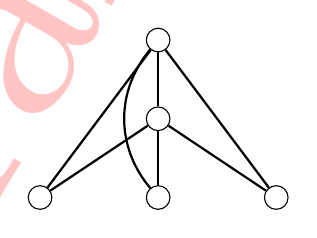
\begin{tikzpicture}[x=4cm, y=2cm, scale = 0.25]
        \tikzset{     
        e4c node/.style={circle,draw,minimum size=0.3cm,inner sep=0}, 
        e4c edge/.style={sloped,above,font=\footnotesize}
        }
        \node[e4c node] (1) at (0, 0) {};
        \node[e4c node] (2) at (0, -2) {};
        \node[e4c node] (3) at (-1.5, -4) {};
        \node[e4c node] (4) at (0, -4) {};
        \node[e4c node] (5) at (1.5, -4) {};

        \path[-,draw,thick]
        (1) edge[e4c edge] (2)
        (1) edge[e4c edge] (3)
        (1) edge[e4c edge] (5)
        (2) edge[e4c edge] (3)
        (2) edge[e4c edge] (4)
        (2) edge[e4c edge] (5)
        (4) edge[e4c edge, bend left = 40] (1)
        ;
    \end{tikzpicture}
    \qquad
    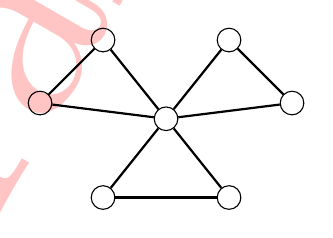
\begin{tikzpicture}[x=4cm,y=2cm]
        \tikzset{     
        e4c node/.style={circle,draw,minimum size=0.3cm,inner sep=0}, 
        e4c edge/.style={sloped,above,font=\footnotesize}
        }
        \node[e4c node] (1) at (3.6, 0.6) {}; 
        \node[e4c node] (2) at (3.8, 1.0) {}; 
        \node[e4c node] (3) at (3.8, 0.0) {}; 
        \node[e4c node] (4) at (4.0, 0.5) {};
        \node[e4c node] (5) at (4.2, 0.0) {};
        \node[e4c node] (6) at (4.2, 1.0) {};
        \node[e4c node] (7) at (4.4, 0.6) {};
        
        \path[-,draw,thick]
        (1) edge[e4c edge] (2)
        (1) edge[e4c edge] (4)
        (2) edge[e4c edge] (4)
        (3) edge[e4c edge] (4)
        (3) edge[e4c edge] (5)
        (4) edge[e4c edge] (5)
        (4) edge[e4c edge] (6)
        (4) edge[e4c edge] (7)
        (6) edge[e4c edge] (7)
        ;
    \end{tikzpicture}
    \end{center}

    \begin{enumerate}[\bf A.]
        \item W dopełnieniach obydwu grafów ich środkowy wierzchołek będzie odizolowany, więc nie może istnieć tam cykl Hamiltona.

        \item Graf po prawej nie ma ścieżki Hamiltona.

        \item Graf po lewej jest dwuspójny, więc posiada tylko jedną dwuspójną składową -- samego siebie.
    \end{enumerate}

    % Wiktor
    \sol Każdy graf nieplanarny o $n$ wierzchołkach
    \answerss{zawiera podgraf $K_{3,3}$ lub $K_5$}{ma co najmniej $3n-5$ krawędzi}{ma liczbę chromatyczną nie mniejszą niż 5}{NIE}{NIE}{NIE}
    \begin{enumerate}[\bf A.]
        \item Graf nieplanarny jest z $K_5$ lub $K_{3,3}$ homeomorficzny, ale nie oznacza to, że któryś z nich jest jego podgrafem.
        \item Kontrprzykładem jest $K_{3, 3}$ (9 krawędzi, 6 wierzchołków).
        \item Wiemy, że jeśli graf jest planarny, to jego liczba chromatyczna jest mniejsza bądź równa 4, ale nie jest to implikacja obustronna. Graf $K_{3,3}$ ma liczbę chromatyczną $2$.
    \end{enumerate}

    % Patryk
    \sol Graf $100$-wierzchołkowy $G$ ma liczbę chromatyczną $3$. Wynika z tego, że graf $G$
    \answerss{jest planarny}{zawiera cykl}{zawiera niezależny zbiór wierzchołków rozmiaru $34$}{NIE}{TAK}{TAK}

    Możemy o takim grafie pomyśleć jak o grafie \textit{trójdzielnym} -- dzielimy 100 wierzchołków na 3 zbiory, każdy odpowiadający jednemu kolorowi. Krawędź może wystąpić tylko między wierzchołkami o różnych kolorach (wynika to wprost z definicji kolorowania grafu).

    \begin{enumerate}[\bf A.]
        \item Weźmy oszacowanie na liczbę krawędzi w grafie planarnym: $e \leq 3v-6$. Wynika z niego, że w grafie $G$ mogą być co najwyżej 294 krawędzie. Weźmy graf, w którym są 33 wierzchołki niebieskie, 33 zielone i 34 czerwone. Połączmy ze sobą wszystkie niebieskie i zielone wierzchołki, otrzymując $33^2 = 1089 > 294$ krawędzi, więc taki graf nie jest planarny.

        \item Gdyby graf $G$ nie zawierał cyklu, jego liczba chromatyczna byłaby równa 2 (moglibyśmy pokolorować wierzchołki dwoma kolorami, na przemian) -- sprzeczność z założeniem.

        \item Przy podzieleniu 100 wierzchołków na 3 zbiory, jeden z nich będzie miał moc co najmniej 34 (zasada szufladkowa), więc można znaleźć w nim podzbiór 34 niezależnych wierzchołków.
    \end{enumerate}
    
    % Julia
    \sol Dany jest $k$-regularny graf o $n$ wierzchołkach i $m$ krawędziach. Wtedy
    \answerss
    {$k$ jest parzyste lub $n$ jest parzyste}
    {$k$ jest dzielnikiem $n$}
    {$k$ jest dzielnikiem $m$}
    {TAK}{NIE}{NIE}

    \begin{enumerate}[\bf A.]
        \item Z definicji $k$-regularnego grafu wiemy, że z każdego wierzchołka wychodzi $k$ krawędzi. Z lematu o uściskach dłoni otrzymujemy równanie $kn = 2m$. Ponieważ $m$ jest liczbą naturalną, $k$ lub $n$ musi być parzyste.
        \item Kontrprzykładem jest $K_5$.
        \item Kontrprzykładem jest $K_3$.
    \end{enumerate}

    % Grześ
    \sol $G$ jest grafem spójnym o $n > 2$ wierzchołkach i takim, że każda jego krawędź należy do pewnego cyklu prostego. Wynika z tego, że
    \answerss
    {$G$ ma cykl Hamiltona}
    {graf otrzymany przez usunięcie z $G$ jednego wierzchołka jest spójny}
    {każde dwa różne wierzchołki w $G$ są połączone przynajmniej dwiema krawędziowo rozłącznymi ścieżkami}
    {NIE}{NIE}{TAK}
    Rozważmy następujący graf spełniający warunki zadania:
    \begin{center}
        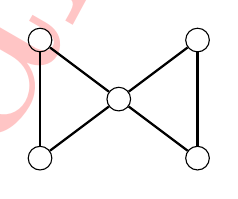
\begin{tikzpicture}[x=2cm,y=1.5cm]
            \tikzset{     
            e4c node/.style={circle,draw,minimum size=0.3cm,inner sep=0}, 
            e4c edge/.style={sloped,above,font=\footnotesize}
            }
            \node[e4c node] (1) at (3.4, 1.0) {}; 
            \node[e4c node] (2) at (3.4, 0.0) {}; 
            \node[e4c node] (3) at (3.9, 0.5) {}; 
            \node[e4c node] (4) at (4.4, 0.0) {};
            \node[e4c node] (5) at (4.4, 1.0) {};
            
            \path[-,draw,thick]
            (1) edge[e4c edge] (2)
            (1) edge[e4c edge] (3)
            (2) edge[e4c edge] (3)
            (3) edge[e4c edge] (4)
            (3) edge[e4c edge] (5)
            (4) edge[e4c edge] (5)
            ;
        \end{tikzpicture}
    \end{center}
    
    Nietrudno sprawdzić, że nie ma on cyklu Hamiltona, a po usunięciu środkowego wierzchołka graf się rozspójni. Wobec tego odpowiedzi \textbf{A.} i \textbf{B.} są fałszywe. 
    
    Zauważmy, że w grafie $G$ danym w treści zadania nie mogą wystąpić mosty (krawędzie rozspójniające) -- gdyby w grafie był most, krawędź ta musiałaby należeć do cyklu prostego, co jest niemożliwe, gdyż po przejściu przez most nie jesteśmy już w stanie ,,wrócić'', żeby zamknąć cykl. Skoro nie ma mostów, to usunięcie dowolnej krawędzi z grafu go nie rozspójnia.
    
    Weźmy więc ścieżkę pomiędzy dowolnymi dwoma wierzchołkami $u$ i $v$. Usuwając wszystkie krawędzie na ścieżce, graf wciąż jest spójny, więc istnieje druga, rozłączna krawędziowo z pierwszą, ścieżka z $u$ do $v$. Stąd odpowiedź w \textbf{C.} to \texttt{TAK}.

    % Wiktor
    \sol Graf $G$ ma $n > 2$ wierzchołków i $n$ krawędzi. Wynika z tego, że graf $G$
    \answerss
    {jest spójny}
    {zawiera cykl}
    {jest planarny}
    {NIE}{TAK}{NIE}
    
    \begin{enumerate}[\bf A.]
        \item Nie musi tak być -- weźmy $K_4$ (4 wierzchołki, 6 krawędzi) i dorzućmy dwa izolowane wierzchołki.
        \item Gdyby $G$ nie zawierał żadnego cyklu, to byłby drzewem. Jak wiemy, drzewa to spójne grafy spełniające zależność $|V| = |E| + 1$, więc w naszym przypadku, chcąc dołożyć $n$-tą krawędź, utworzylibyśmy cykl.
        \item Kontrprzykład: bierzemy $K_5$ i dokładamy tyle izolowanych wierzchołków, żeby ich liczba była równa liczbie krawędzi.
    \end{enumerate}

    \sol $G$ jest $n$-wierzchołkowym grafem spójnym regularnym stopnia 3. Wynika z tego, że
    \answerss{$n$ jest parzyste}{$G$ jest planarny}{liczba chromatyczna $\chi(G) \leq 4$}
    {TAK}{NIE}{TAK}

    \begin{enumerate}[\bf A.]
        \item Oznaczmy przez $m$ liczbę krawędzi grafu z zadania. Z lematu o uściskach dłoni otrzymujemy zależność $3n = 2m$ i -- ponieważ $n$ i $m$ to liczby naturalne -- nietrudno zauważyć, że $n$ musi być parzyste.
        
        \item Kontrprzykładem jest $K_{3, 3}$.

        \item Ponieważ każdy wierzchołek grafu $G$ jest połączony z dokładnie trzema innymi, mamy pewność, że wystarczą nam 4 barwy do prawidłowego pokolorowania grafu. 
    \end{enumerate}

    % Grześ
    \sol Liczba $p > 2$ jest pierwsza. Wynika z tego, że
    \answerss{$(p-2)^{p-1}-1$ dzieli się przez $p$}{$(p-2)^{p^2-1}-1$ dzieli się przez $p^2$}{$(p-2)^{p^3-p^2}-1$ dzieli się przez $p^3$}{TAK}{NIE}{TAK}
    Nietrudno zauważyć, że $(p-2)\perp p$. Możemy więc skorzystać z małego twierdzenia Fermata, otrzymując ${(p-2)^{p-1}\equiv 1\mod{p}}$. Zatem podpunkt \textbf{A.} jest prawdziwy.
    
    Skoro $(p-2)\perp p$, to również $(p-2)\perp p^3$ oraz $\Phi(p^3)=p^3-p^2$, bo $p$ jest pierwsze. Z twierdzenia Eulera dostajemy $(p-2)^{p^3-p^2}\equiv 1\mod{p^3}$, więc podpunkt \textbf{C.} również jest prawdziwy.
    
    Do podpunktu \textbf{B.} posłuży nam kontrprzykład: weźmy najmniejszą (sensowną) liczbę pierwszą $p=5$. Obliczamy:
    \begin{align*}
        (p-2)^{p^2-1} &\mod p^2 \\
        (5-2)^{25-1} &\mod 25 \\
        3^{24} &\mod 25
    \end{align*}
    Widzimy, że $3^3\equiv 27\equiv 2\mod{25}$. Podnosimy tę kongruencję stronami do potęgi 8 i dostajemy $3^{24}\equiv 2^8\equiv 256\equiv 6\nequiv 1\mod{25}$. Odpowiedź jest więc fałszywa.

    % Jasiek
    \sol Jeśli $a, b$ są dodatnimi liczbami całkowitymi, to $\mathrm{NWD}(a,b)$ jest najmniejszym dodatnim elementem zbioru
    \answerss{$\{ax + by \mid x, y \in \mathbb{Z}\}$}{$\{a(x+y) + b(x-y) \mid x, y \in \mathbb{Z}\}$}{$\{2ax + 3by \mid x,y \in \mathbb{Z}\}$}{TAK}{NIE}{NIE}
    Prawdziwa odpowiedź do podpunktu \textbf{A.} wynika wprost z definicji NWD. W podpunkcie \textbf{B.} rozważmy $a = 9, b = 15$ (wtedy NWD$(a, b) = 3$). Dla pewnych $x, y$ musi zachodzić:
    \begin{align*}
        9(x + y) + 15(x - y) = 3 \wtw 3(x + y) + 5(x - y) = 1 \wtw 8x - 2y = 1
    \end{align*}
    To prowadzi do sprzeczności, ponieważ po lewej stronie równości znajduje się liczba nieparzysta, a~po prawej parzysta.
    
    W podpunkcie \textbf{C.} przeprowadzamy taką samą argumentację dla $a = 2, b = 4$ i~ponownie uzyskujemy sprzeczność: $$4x + 12y = 2 \wtw 2x + 6y = 1$$
    
    % Grześ
    \sol Dane są dodatnie liczby całkowite $a, b$, których największy wspólny dzielnik jest równy $d$. Wówczas względnie pierwsze są liczby
    \answerss{$\frac{a}{d}$ oraz $b$}{$\frac{ab}{d^2}$ oraz $b$}{$\frac{a^2}{d^2}$ oraz $\frac{b^2}{d^2}$}{NIE}{NIE}{TAK}
    
    Połóżmy $a=d\cdot a'$ i $b=d\cdot b'$, gdzie $d$ to $\mathrm{NWD}(a,b)$. Oczywiście $a'\perp b'$. Podpunkt \textbf{A.} jest fałszywy, bo o ile $a'\perp b'$, to nieprawdą jest, że $a'\perp d$; nie musi tak być chociażby dla $a=2^2$ i $b=2\cdot3$. Ten przykład pokazuje również, że \textbf{B.} nie ma sensu (z tego samego powodu).
    
    Podpunkt \textbf{C.} jest jednak prawdziwy, gdyż $\frac{a^2}{d^2}=(a')^2$, $\frac{b^2}{d^2}=(b')^2$, a skoro $a'\perp b'$, to oczywiście $(a')^2\perp (b')^2$.

    % Patryk
    \sol Funkcje $f, g: \NN \rightarrow \RR$ przyjmują wyłącznie wartości dodatnie i są niemalejące. Wynika z tego, że
    \answerss{jeśli $f = O(g)$ i $g = O(f)$, to istnieje skończona granica $\Limn \frac{f(n)}{g(n)}$}{jeśli $f = O(g)$, to $f/g = O(1)$}{$f = O(g)$ lub $g = O(f)$}{NIE}{TAK}{NIE}

    \begin{enumerate}[\bf A.]
        \item Taka granica nie musi istnieć. Kontrprzykładem mogą być funkcje
        $$f(n) = n, \qquad g(n) = \begin{cases}
            n & \text{dla } n \text{ nieparzystych,} \\
            2n & \text{dla } n \text{ parzystych.}
        \end{cases}$$
        
        \item Z definicji notacji asymptotycznej mamy, że dla pewnej stałej $c$ i dostatecznie dużych $n$ zachodzi $$f(n) \leq c \cdot g(n), \quad \text{ a stąd } \quad \frac{f(n)}{g(n)} \leq c.$$ 

        \item Rozważmy funkcje
        $$
        f(n) = 
        \begin{cases}
            (n - 1)^2 & \text{dla } n \text{ nieparzystych,} \\
            n^2 & \text{dla } n \text{ parzystych,}
        \end{cases}
        $$
    
        $$
        g(n) = 
        \begin{cases}
            n^2 & \text{dla } n \text{ nieparzystych,} \\
            (n - 1)^2 & \text{dla } n \text{ parzystych,}
        \end{cases}
        $$
        będące ciągami kwadratowymi, przy czym raz rośnie $f$, a raz $g$. Wówczas różnica $|f(n)-g(n)|$ wraz ze wzrostem $n$ dąży do nieskończoności oraz $\big(f(n)-g(n)\big)\big(f(n+1)-g(n+1)\big) < 0$.
    \end{enumerate}

    % Grześ
    \sol Rozwiązaniem równania rekurencyjnego $T(n)=2T(\lfloor n/2 \rfloor)+f(n)$ dla $n>1$, $T(1)=0$, jest
    \answerss{$T(n)=\Theta(\log{n})$, jeśli $f(n)=O(1)$}{$T(n)=\Theta(n)$, jeśli $f(n)=\Theta(\sqrt{n})$}{$T(n)=\Theta(n^2)$, jeśli $f(n)=\Theta(n^2)$}{NIE}{TAK}{TAK}
    
    Korzystamy z twierdzenia o rekurencji uniwersalnej. Odczytujemy $a=b=2$, więc nasze $f(n)$ musimy dopasować do jednego z trzech przypadków:
    \begin{enumerate}[1.]
        \item $f(n)=O(n^{\log_b{a}-\epsilon})=O(n^{1-\epsilon})$,
        \item $f(n)=\Theta(n^{\log_b{a}})=\Theta(n)$,
        \item $f(n)=\Omega(n^{\log_b{a}+\epsilon})=\Omega(n^{1+\epsilon})$.
    \end{enumerate}

    \begin{enumerate}[\bf A.]
        \item Skoro $f(n)=O(1)$, to otrzymujemy pierwszy przypadek. Rozwiązaniem równania rekurencyjnego będzie $T(n)=\Theta(n^{\log_ba})=\Theta(n)$, czyli odpowiedź to \texttt{NIE}.

        \item Skoro $f(n)=\Theta(\sqrt{n})$, to znów jesteśmy w przypadku pierwszym i rozwiązaniem jest $T(n)=\Theta(n)$, czyli odpowiedź to \texttt{TAK}.

        \item Jeśli $f(n)=\Theta(n^2)$, to wpadamy do trzeciego przypadku, więc rozwiązaniem jest $T(n)=\Theta(f(n))=\Theta(n^2)$, czyli \texttt{TAK}.
    \end{enumerate}
\end{solutions}

\chapter{Rachunek prawdopodobieństwa}

Materiały teoretyczne zostały opracowane na podstawie \href{https://drive.google.com/file/d/1WlyT05bbN8DMYJ59sRA7HeTXgpvc7yQ4/view}{notatek Błażeja Wilkoławskiego}, \href{https://wazniak.mimuw.edu.pl/index.php?title=Rachunek_prawdopodobie%C5%84stwa_i_statystyka}{materiałów na Ważniaku} oraz \href{https://www.mimuw.edu.pl/~ados/MNRP/MNRP.pdf}{skryptu z Metodyki Nauczania Rachunku Prawdopodobieństwa autorstwa Adama Osękowskiego}.

\section*{Podstawa programowa}
\begin{enumerate}
    \item \textbf{Prawdopodobieństwo warunkowe i całkowite}, wzór Bayesa, niezależność zdarzeń.
    \item \textbf{Dyskretne zmienne losowe} i ich rozkłady: dwumianowy, geometryczny, Poissona.
    \item \textbf{Parametry rozkładu}: wartość oczekiwana, wariancja, funkcje tworzące prawdopodobieństwa.
    \item \textbf{Nierówności probabilistyczne}: Markowa, Czebyszewa, Chernoffa.
    \item \textbf{Ciągłe zmienne losowe}: definicja, własności, rozkład wykładniczy oraz normalny, centralne twierdzenie graniczne.
    \item \textbf{Łańcuchy Markowa}: prawdopodobieństwa oraz średnie czasy dotarcia, twierdzenie ergodyczne.
    \item \textbf{Wnioskowanie statystyczne}: estymatory nieobciążone, estymatory największej wiarygodności.
\end{enumerate}

\section{Prawdopodobieństwo warunkowe i całkowite}

\textbf{Doświadczeniem losowym} nazwiemy dowolny proces bądź ciąg czynności taki, że:
\begin{itemize}
    \item jego sposób wykonania i warunki są ściśle określone, a sam proces można dowolnie wiele razy powtarzać,
    \item zbiór możliwych wyników procesu (\textbf{zdarzeń elementarnych}) jest z góry znany,
    \item wyniku konkretnego doświadczenia nie można z góry przewidzieć.
\end{itemize}

Zbiór wszystkich zdarzeń elementarnych oznaczamy wielką literą $\Omega$.

W wielu sytuacjach interesuje nas nie tyle konkretny wynik doświadczenia (pojedyncze zdarzenie elementarne), ale to, czy należy on do wcześniej ustalonego podzbioru wszystkich zdarzeń elementarnych. Takie podzbiory nazywamy \textbf{zdarzeniami} i zwyczajowo oznaczamy wielkimi literami alfabetu, np. $A, B, X, Y...$

\begin{example}
    Dla doświadczenia losowego będącego rzutem kostką, zbiorem zdarzeń elementarnych jest $\Omega = \{1, 2, ..., 6\}$, a przykładowymi zdarzeniami:
    \begin{itemize}
        \item $A = \{2, 4, 6\}$ -- wypadła liczba parzysta
        \item $B = \{1, 2, 3, 4, 5, 6\}$ -- coś wypadło
        \item $C = \pusty$ -- nic nie wypadło
    \end{itemize}
\end{example}

\textit{Uwaga:} ponieważ w programie studiów informatycznych nie zajmujemy się innym prawdopodobieństwem niż prawdopodobieństwo klasyczne, pominiemy tutaj formalizmy związane z przestrzeniami probabilistycznymi -- nie są one potrzebne przy rozwiązywaniu zadań. Zaznaczymy jedynie, że przestrzenie te służą do definiowania sposobu przypisania poszczególnym zdarzeniom ich prawdopodobieństw.

\subsection{Podstawowe własności prawdopodobieństwa}

Niech $\Omega$ będzie niepustym zbiorem wszystkich zdarzeń elementarnych doświadczenia losowego, a $P$ -- prawdopodobieństwem określonym na podzbiorach $\Omega$. Wtedy:
\begin{itemize}
    \item dla każdego zdarzenia $A$ zachodzi $P(A) \in [0, 1]$, przy czym $P(\pusty) = 0$ oraz $P(\Omega) = 1$
    \item dla dowolnych zdarzeń $A, B$, takich że $A \subseteq B$, jest $P(A) \leq P(B)$
    \item $P(A') = 1 - P(A)$, gdzie $A'$ to zdarzenie przeciwne do zdarzenia $A$
    \item dla dowolnych zdarzeń $A, B$ mamy $$P(A \cup B) = P(A) + P(B) - P(A \cap B)$$
\end{itemize}

\begin{wrapfigure}{r}{5cm}
    \vspace{-5mm}
    
    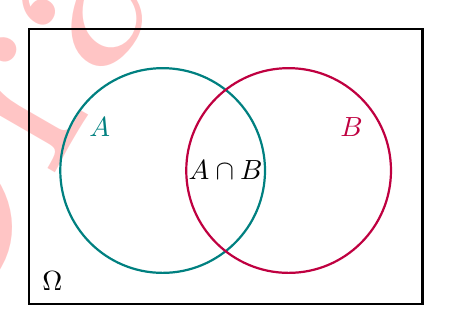
\begin{tikzpicture}
        \draw[black, thick] (-1.5,-1.5) rectangle (3.5,2);
        \draw[teal, thick] (0.2,0.2) circle (1.3);
        \draw[purple, thick] (1.8,0.2) circle (1.3);
    
        % Etykiety
        \node at (-0.6, 0.75) {$\teal{A}$};
        \node at (2.6, 0.75) {$\purple{B}$};
        \node at (-1.2, -1.2) {$\Omega$};
        \node at (1, 0.2) {$A \cap B$};
    \end{tikzpicture}
\end{wrapfigure}

Przydatnym trikiem jest \purple{wizualizacja geometryczna} przestrzeni probabilistycznej za pomocą \textbf{diagramów Venna}, czyli schematów służących ilustrowaniu zależności między zbiorami (w naszym przypadku -- między zdarzeniami).

Z rysunku łatwo odczytać na przykład powyższy wzór na prawdopodobieństwo sumy zdarzeń $P(A \cup B)$ oraz wiele innych nieoczywistych relacji, jak np.
$$P(A' \cup B) = 1 - P(A \setminus B)$$

\subsection{Schemat klasyczny}

Aby móc wygodnie obliczać prawdopodobieństwa interesujących nas zdarzeń, w większości przypadków będziemy sprowadzać całe rozumowanie do problemu kombinatorycznego za pomocą \textbf{schematu klasycznego}.

Załóżmy, że $\Omega$ jest zbiorem skończonym i wszystkie zdarzenia elementarne są jednakowo prawdopodobne. Wówczas dla każdego $\omega \in \Omega$ oraz $A \subseteq \Omega$ zachodzi
$$\purple{P(\omega) = \frac{1}{|\Omega|}} \textqq{oraz} \purple{P(A) = \frac{|A|}{|\Omega|}}$$

\begin{example}
    Obliczymy prawdopodobieństwo, że w losowej 5-kartowej ręce pokerowej jest dokładnie jedna para (w szczególności nie ma w niej żadnej trójki ani dwóch par).
    
    W naszym przypadku $\Omega$ to zbiór wszystkich 5-elementowych podzbiorów 52 kart, mamy więc $|\Omega| = \binom{52}{5}$. Niech $A$ będzie zbiorem wszystkich układów z dokładnie jedną parą. Ponieważ każdy 5-elementowy podzbiór kart jest równie prawdopodobny, korzystamy ze schematu klasycznego i dostajemy $P(A)=\frac{|A|}{|\Omega|}$.
    
    Sprawdźmy, na ile sposobów można wybrać jedną parę:
    \begin{enumerate}
        \item na 13 sposobów wybieramy rangę kart w parze,
        \item na $\binom{4}{2}=6$ sposobów wybieramy kolory tych kart,
        \item na $\binom{12}{3}$ sposobów wybieramy rangi pozostałych kart (muszą być różne),
        \item na $4^3$ sposobów wybieramy kolory tych kart.
    \end{enumerate}
    Ostatecznie $|A|=13\cdot6\cdot\binom{12}{3}\cdot4^3$ oraz $P(A)\approx0,423$. Jak widać, użycie schematu klasycznego sprowadziło problem probabilistyczny do problemu kombinatorycznego.
\end{example}

\subsection{Prawdopodobieństwo warunkowe i całkowite}

Na początek przytoczymy przykład, który pozwoli nam przybliżyć intuicję idącą za prawdopodobieństwem warunkowym. 

Przypuśćmy, że rzucamy dwukrotnie kostką ,,na ślepo'' (nie patrząc na wyniki) i ktoś stojący obok mówi nam, że w sumie wyrzuciliśmy osiem oczek. Jakie jest prawdopodobieństwo, że w pierwszym rzucie kostką uzyskaliśmy dwójkę lub trójkę?

Jasne jest, iż nie dysponując dodatkową informacją o sumie oczek podalibyśmy odpowiedź $\frac{1}{3}$ (dokładnie 12 z 36 możliwych zdarzeń elementarnych spełnia postawiony warunek). Jednak skoro wiemy, że suma oczek wynosi 8, to musiała zajść jedna z pięciu możliwości:
$$(2, 6), (3, 5), (4, 4), (5, 3), (6, 2).$$
Ponieważ w dokładnie dwóch z nich na pierwszej współrzędnej stoi dwójka lub trójka, widzimy, że szukane prawdopodobieństwo wynosi $\frac{2}{5}$.

Ten przykład dobrze pokazuje intuicję stojącą za \textbf{prawdopodobieństwem warunkowym} -- szukamy prawdopodobieństwa zajścia zdarzenia $A$ pod warunkiem zajścia zdarzenia $B$, oznaczanego $P(A | B)$.

Skoro zaszło zdarzenie $B$ i interesuje nas zdarzenie $A$, to w rzeczywistości muszą zajść oba zdarzenia $A$ i $B$ ($A \cap B$). Ponadto, skoro zaszło zdarzenie $B$, to zbiór $B$ staje się naszą nową, zredukowaną przestrzenią zdarzeń elementarnych (jak w przykładzie). To rozumowanie daje nam naturalną definicję
$$\purple{P(A | B) = \frac{P(A \cap B)}{P(B)}}$$
Zakładamy przy tym, że $P(B) > 0$.
\bigskip

Warto przytoczyć również \textbf{wzór iloczynowy}, pozwalający wyrazić prawdopodobieństwo iloczynu zdarzeń przez iloczyn odpowiednich prawdopodobieństw warunkowych.

Niech $A_1, A_2, ..., A_n \subseteq \Omega$ oraz $P(A_1 \cap A_2 \cap ... \cap A_n)>0$. Wtedy
$$
\purple{P(A_1 \cap A_2 \cap ... \cap A_n)=P(A_1)\cdot P(A_2|A_1)\cdot P(A_3|A_1\cap A_2)\cdot\ldots\cdot P(A_n|A_1\cap\ldots\cap A_{n-1})}
$$

\begin{example}
    Test na obecność koronawirusa ma skuteczność 95\%. Wiadomo, że średnio 1 na 1000 osób jest zakażona. Jeśli dla losowo wybranej osoby test dał wynik pozytywny, to jakie jest prawdopodobieństwo, że jest ona faktycznie chora?
    
    Oznaczmy:
    \begin{itemize}
        \item $C$ -- wybrana osoba jest chora,
        \item $Z$ -- wybrana osoba jest zdrowa,
        \item $T$ -- test da wynik pozytywny,
        \item $N$ -- test da wynik negatywny.
    \end{itemize}
    Naszym celem jest obliczenie $P(C|T)$. Z treści wiemy, że $P(T|C)=0,95$, $P(N|C)=0.05$, $P(T|Z)=0.05$, $P(N|Z)=0.95$. Korzystając ze wzoru iloczynowego, możemy znaleźć szukane prawdopodobieństwo:
    $$
    P(C|T) = \frac{P(C\cap T)}{\underbrace{P(T)}_{P(C\cap T)+P(Z\cap T)}} = \frac{P(C)P(T|C)}{P(C)P(T|C)+P(Z)P(T|Z)} = \frac{0.001\cdot0.95}{0.001\cdot0.95+0.999\cdot0.05} \approx 0.02.
    $$
\end{example}

Sposób, w jaki w powyższym przykładzie obliczyliśmy $P(T)$, to szczególny przypadek \textbf{twierdzenia o prawdopodobieństwie całkowitym}. Używamy go w szczególności do badania wyników doświadczeń, które składają się z kilku etapów.

Niech $A_1, A_2, ..., A_n \subset \Omega$ będą takie, że $P(A_i)>0$ i
\begin{itemize}
    \item $A_i\cap A_j=\varnothing$ (wszystkie $A_i$ są parami rozłączne),
    \item $A_1\cup\ldots\cup A_n=\Omega$ (wszystkie $A_i$ pokrywają $\Omega$)
\end{itemize}
Wówczas dla dowolnego zdarzenia $B \subseteq \Omega$ zachodzi wzór
$$\purple{P(B) = P(B|A_1)P(A_1)+\ldots+P(B|A_n)P(A_n)}$$

\begin{example}
    W urnie znajdują się dwie białe kule i jedna czarna. Losujemy kulę (nie oglądamy jej) i odkładamy na bok. Następnie losujemy drugą kulę. Jakie jest prawdopodobieństwo, że druga kula jest biała?

    Opisane doświadczenie składa się z dwóch etapów, będących wylosowaniem odpowiednio pierwszej i drugiej kuli z urny. Są dwa możliwe wyniki pierwszego etapu:
    \begin{itemize}
        \item $B_1$ -- jako pierwszą wylosowano kulę białą,
        \item $C_1$ -- jako pierwszą wylosowano kulę czarną.
    \end{itemize}
    W oczywisty sposób są to rozłączne przypadki oraz pokrywają wszystkie możliwości (nie ma innych kul niż białe i czarne) -- spełniają więc założenia twierdzenia o prawdopodobieństwie całkowitym.

    Oznaczmy szukane zdarzenie (,,jako drugą wylosowano kulę białą'') jako $B_2$ i obliczmy jego prawdopodobieństwo:
    $$P(B_2) = P(B_2 | B_1) \cdot P(B_1) + P(B_2 | C_1) \cdot P(C_1) = \frac{1}{2} \cdot \frac{2}{3} + 1 \cdot \frac{1}{3} = \frac{2}{3}$$
\end{example}

Twierdzenie o prawdopodobieństwie całkowitym pomagało nam przy badaniu wyników doświadczeń wieloetapowych. A co w przypadku, gdy znamy wynik takiego doświadczenia, a pytamy o jego przebieg?

W takich sytuacjach wykorzystujemy \textbf{wzór Bayesa}:
niech $B,A_1,\ldots,A_n\subset\Omega$ będą jak w twierdzeniu o prawdopodobieństwie całkowitym. Dla dowolnego $k$ zachodzi
$$
\purple{P(A_k|B) = \frac{P(A_k\cap B)}{P(B)} = \frac{P(A_k)P(B|A_k)}{\sum_{i=1}^n P(A_i)P(B|A_i)}}
$$

\begin{example}
    Kontynuujemy poprzedni przykład z urną i kulami. Załóżmy, że druga wylosowana kula jest biała. Jakie jest prawdopodobieństwo, że jako pierwszą wyciągnięto kulę czarną?

    Przy zachowaniu tych samych oznaczeń zdarzeń, interesuje nas prawdopodobieństwo warunkowe $P(C_1 | B_2)$. Korzystając ze wzoru Bayesa, łatwo obliczamy:
    $$P(C_1 | B_2) = \frac{P(C_1 \cap B_2)}{P(B_2)} = \frac{P(C_1)P(B_2 | C_1)}{P(C_1)P(B_2 | C_1) + P(B_1)P(B_2 | B_1)} = \frac{\frac{1}{3} \cdot 1}{\frac{2}{3}} = \frac{1}{2}$$
\end{example}

\subsection{Metoda drzewkowa}

W sytuacji, gdy badane doświadczenie składa się z większej liczby etapów, warto zilustrować je za pomocą odpowiedniego \textbf{drzewa} -- w ten sposób, zamiast algebraicznie wyliczać prawdopodobieństwo całego zdarzenia, możemy rozpatrzeć wszystkie możliwe losowania za pomocą rysunku. Ze wzoru iloczynowego wynika, że prawdopodobieństwo znalezienia się w konkretnym wierzchołku jest równe iloczynowi liczb na ścieżce od korzenia do tego wierzchołka.

\begin{example}
    Mamy dwie urny z pewną (znaną) liczbą kul białych i czarnych. Wybieramy losowo urnę, a następnie losujemy z niej dwie kule. Jakie jest prawdopodobieństwo, że obie z nich będą białe?

    Oznaczmy zdarzenia: $U_1,U_2$ -- wylosowana urna, $B_1,C_1$ -- kolor pierwszej kuli, $B_2,C_2$ -- kolor drugiej kuli. Rozwiązanie algebraiczne wyglądałoby tak:
    $$
    P(B_1\cap B_2) = P(U_1\cap B_1\cap B_2) + P(U_2\cap B_1\cap B_2) = P(U_1)P(B_1|U_1)P(B_2|B_1\cap U_1) + P(U_2)P(B_1|U_2)P(B_2|B_1\cap U_2)
    $$
    Metoda drzewkowa:
    \begin{center}
    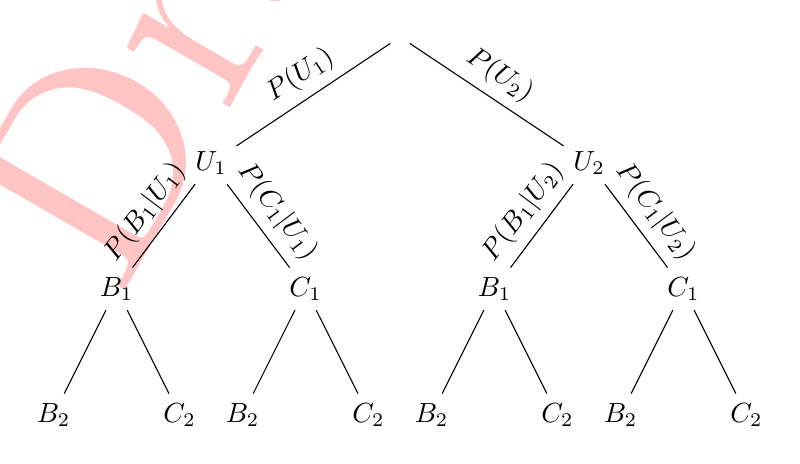
\begin{tikzpicture}[sloped,
                        level distance=2cm,
                        level 1/.style={sibling distance=6cm},
                        level 2/.style={sibling distance=3cm},
                        level 3/.style={sibling distance=2cm},
                        scale = 0.8]
    \node[] {}
    child {
        node[] {$U_1$}
        child {
          node[] {$B_1$}
          child {
            node[] {$B_2$}
          }
          child {
            node[] {$C_2$}
          }
          edge from parent
          node[above] {$P(B_1|U_1)$}
        }
        child {
          node[] {$C_1$}
          child {
            node[] {$B_2$}
          }
          child {
            node[] {$C_2$}
          }
          edge from parent
          node[above] {$P(C_1|U_1)$}
        }
        edge from parent
        node[above] {$P(U_1)$}
    }
    child {
        node[] {$U_2$}
        child {
          node[] {$B_1$}
          child {
            node[] {$B_2$}
          }
          child {
            node[] {$C_2$}
          }
          edge from parent
          node[above] {$P(B_1|U_2)$}
        }
        child {
          node[] {$C_1$}
          child {
            node[] {$B_2$}
          }
          child {
            node[] {$C_2$}
          }
          edge from parent
          node[above] {$P(C_1|U_2)$}
        }
        edge from parent
        node[above] {$P(U_2)$}
    };
    \end{tikzpicture}
    \end{center}
    Aby znaleźć $P(B_1\cap B_2)$ za pomocą powyższego drzewa, sumujemy $P(U_1\cap B_1\cap B_2)$ i $P(U_2\cap B_1\cap B_2)$, mnożąc liczby na odpowiednich ścieżkach w drzewie.
\end{example}

\subsection{Schemat Bernoulliego}

\textbf{Schematem Bernoulliego} nazywamy ciąg niezależnych powtórzeń tego samego doświadczenia, w którym możliwe są dwa wyniki: jeden z nich nazywamy \textbf{sukcesem} (o prawdopodobieństwie $p$), a drugi \textbf{porażką} (o prawdopodobieństwie $1 - p$). Pojedyncze doświadczenie nazywamy \textbf{próbą Bernoulliego}.

Taki schemat jest jednoznacznie określony przez podanie liczby prób (oznaczanej $n$) i prawdopodobieństwa sukcesu $p$. Można też rozpatrywać schematy Bernoulliego z nieskończoną liczbą prób.

Nietrudno kombinatorycznie pokazać, że prawdopodobieństwo uzyskania dokładnie $k$ sukcesów w schemacie Bernoulliego składającego się z $n$ prób wynosi
$$\purple{\binom{n}{k} p^k (1 - p)^{n - k}}$$
Istotnie, $k$ spośród $n$ prób zakończy się sukcesem (stanie się to z prawdopodobieństwem $p^k$), pozostałe $n - k$ prób zakończy się porażką (prawdopodobieństwo $(1 - p)^{n - k}$), a na $\binom{n}{k}$ sposobów wybieramy, które $k$ prób będzie pomyślne.

\begin{example}
    Rzucamy 10 razy kostką. Znajdziemy prawdopodobieństwo tego, że szóstka wypadnie raz lub dwa razy.

    Oznaczmy poszukiwane zdarzenie jako $A$. Mamy tu do czynienia ze schematem Bernoulliego składającym się z $n = 10$ prób. Próbą Bernoulliego jest pojedynczy rzut kostką, a sukcesem -- wyrzucenie 6 oczek, zatem $p = \frac{1}{6}$. Wobec tego obliczamy
    $$P(A) = \underbrace{\binom{10}{1} \left(\frac{1}{6}\right)^1 \left(\frac{5}{6}\right)^9}_{\text{jeden sukces}} + \underbrace{\binom{10}{2} \left(\frac{1}{6}\right)^2 \left(\frac{5}{6}\right)^8}_{\text{dwa sukcesy}}$$
\end{example}

\subsection{Niezależność zdarzeń}

Na ogół, jeśli zdarzenia $A, B$ są takie, że $P(B) > 0$, to prawdopodobieństwo warunkowe $P(A | B)$ różni się od prawdopodobieństwa bezwarunkowego $P(A)$. Innymi słowy, dodatkowa informacja podana za pomocą zdarzenia $B$ w istotny sposób zmienia szansę zajścia zdarzenia $A$. Czasami jednak to, czy zdarzenie $B$ zaszło czy nie, nie wpływa na prawdopodobieństwo $A$: mamy wtedy $P(A | B) = P(A)$. W takiej sytuacji mówimy, że $A$ i $B$ są \textbf{niezależne}.

Rozpisując wzór na prawdopodobieństwo warunkowe, powyższa równość daje się zapisać w równoważnej postaci stanowiącej definicję niezależności zdarzeń:
$$\purple{P(A \cap B) = P(A) \cdot P(B)}$$

Jeśli powyższa równość nie zachodzi, to powiemy, że zdarzenia $A$ i $B$ są \textbf{zależne}.

O pojęciu niezależności należy więc myśleć w sposób ,,czy zajście zdarzenia $B$ daje mi dodatkową informację na temat zdarzenia $A$?'', a nie w terminach związków fizycznych między zdarzeniami.

\begin{example}
    Z talii 52 kart losujemy kartę. Rozważmy zdarzenia:
    \begin{itemize}
        \item $A$ -- wylosowano króla,
        \item $B$ -- wylosowano kiera.
    \end{itemize}

    Wówczas zdarzenia $A$ i $B$ są niezależne -- łatwo sprawdzamy:
    $$P(A) = \frac{4}{52}, \qquad P(B) = \frac{13}{52} = \frac{1}{4}, \qquad P(A \cap B) = \frac{1}{52} = P(A)P(B)$$
\end{example}

\begin{exam}
    Rzucamy symetrycznymi kostkami: sześcienną i ośmiościenną. Niech $A$ będzie zdarzeniem, że na kostce sześciennej wypadło $6$. Zdarzeniami niezależnymi od $A$ są
    \answers{suma oczek na obu kostkach jest parzysta}{suma oczek na obu kostkach jest równa $7$}{suma oczek na obu kostkach jest większa od $7$}
    \bigskip

    Nietrudno zauważyć, że $|\Omega| = 48$ oraz $P(A) = \frac{1}{6}$. W każdym z podpunktów pozostaje nam zatem policzyć $P(A \cap B)$ oraz $P(B)$ (za $B$ oznaczamy zdarzenie z danego podpunktu), a następnie sprawdzić warunek na niezależność zdarzeń.
    \begin{enumerate}[\bf A.]
        \item Oznaczmy $B$ -- suma oczek na obu kostkach jest parzysta. Jeśli na pierwszej kostce wypadła parzysta liczba oczek, to na drugiej również, analogicznie dla nieparzystych. Mamy więc $|B| = 3 \cdot 4 + 3 \cdot 4 = 24$ oraz $P(B) = \frac{24}{48} = \frac{1}{2}$.
        
        Zdarzenie $A \cap B$ spełniają 4 zdarzenia elementarne: $(6, 2), (6, 4), (6, 6), (6, 8)$. W związku z tym
        $$P(A \cap B) = \frac{4}{48} = \frac{1}{12} = P(A) \cdot P(B)$$
        Zdarzenia $A$ i $B$ są więc niezależne. Intuicyjnie możemy rozumieć to następująco: nieważne, co wypadnie na pierwszej kostce, na drugiej jest zawsze tyle samo opcji.

        \item Oznaczmy $B$ -- suma oczek na obu kostkach jest równa 7. Nietrudno obliczamy:
        $$P(B) = \frac{6}{48}, \qquad P(A \cap B) = \frac{1}{48} = P(A) \cdot P(B)$$
        $A$ i $B$ ponownie są niezależne. Intuicyjnie: nieważne, co wypadnie na pierwszej kostce, na drugiej jest tylko jedna opcja.

        \item Oznaczmy $B$ -- suma oczek na obu kostkach jest większa od 7. Wypisując wszystkie zdarzenia elementarne spełniające ten warunek (pominiemy to w tym przykładzie), otrzymujemy
        $$P(B) = \frac{27}{48} = \frac{9}{16}, \qquad P(A \cap B) = \frac{7}{48} \neq P(A) \cdot P(B)$$
        Tym razem zdarzenia $A$ i $B$ są od siebie zależne. Intuicyjnie: zależnie od tego, co wypadnie na pierwszej kostce, na drugiej będziemy mieli różną liczbę opcji.
    \end{enumerate}
\end{exam}

Niezależność więcej niż dwóch zdarzeń definiujemy na dwa sposoby:
\begin{enumerate}
    \item Zdarzenia $A_1, A_2, ..., A_n$ są \textbf{niezależne parami}, jeśli każde dwa spośród nich są niezależne.

    \item Zdarzenia $A_1, A_2, ..., A_n$ są \textbf{niezależne} (lub \textit{niezależne łącznie}, bądź \textit{niezależne zespołowo}), jeśli dla dowolnego ciągu indeksów $i_1<i_2<\ldots<i_k$ zachodzi $$\purple{P(A_{i_1}\cap\ldots\cap A_{i_k})=P(A_{i_1})\cdot\ldots\cdot P(A_{i_k})}$$
\end{enumerate}

\begin{example}
    Rozważmy dwukrotny rzut sześcienną kostką i zbadajmy niezależność następujących trzech zdarzeń:
    \begin{itemize}
        \item $A$ -- suma oczek wynosi 7,
        \item $B$ -- w pierwszym rzucie uzyskano czwórkę,
        \item $C$ -- w drugim rzucie uzyskano trójkę.
    \end{itemize}

    Nietrudno sprawdzić, że $P(A) = P(B) = P(C) = \frac{1}{6}$. Zauważmy, że zdarzenia $A \cap B$, $A \cap C$, $B \cap C$ możemy zdefiniować tak samo: ,,w pierwszym rzucie wypadła czwórka, w drugim trójka'', stąd
    $$P(A \cap B) = P(A \cap C) = P(B \cap C) = \frac{1}{36}$$
    Widzimy więc, że zdarzenia $A, B, C$ są niezależne parami (każde dwa spośród nich są niezależne).
    \bigskip

    Z drugiej strony, $A \cap B \cap C$ również definiujemy jako ,,w pierwszym rzucie wypadła czwórka, w drugim trójka'', więc
    $$P(A \cap B \cap C) = \frac{1}{36} \neq P(A) \cdot P(B) \cdot P(C)$$
    Zdarzenia $A, B, C$ nie są więc niezależne.
\end{example}

\begin{problems}
    \prob Istnieje przestrzeń probabilistyczna $\Omega$ i zdarzenia $A,B\subseteq\Omega$ takie, że $P(A)=P(B)=\frac{2}{3}$ oraz
    \answers{$A$ i $B$ są niezależne}{$P(A|B)=\frac{1}{3}$}{$P(A|B)\neq P(B|A)$}

    \prob Chcemy rozpalić ognisko, lecz mamy do dyspozycji tylko trzy zapałki. Prawdopodobieństwo rozpalenia ogniska pojedynczą zapałką wynosi $0.4$, dwiema złączonymi zapałkami -- $0.6$, zaś trzema złączonymi zapałkami -- $0.8$. Żeby zmaksymalizować prawdopodobieństwo rozpalenia ogniska, należy
    \answers
    {użyć od razu trzech zapałek}
    {użyć najpierw dwóch zapałek, a potem jednej}
    {używać pojedynczych zapałek}

    \prob Rzucamy 10 razy symetryczną monetą. Wynika z tego, że
    \answers
    {prawdopodobieństwo, że wyrzucimy dokładnie 2 orły jest równe $\frac{45}{1024}$}
    {prawdopodobieństwo, że wyrzucimy orła w ostatnim rzucie pod warunkiem, że we wszystkich 10 rzutach wyrzucimy dokładnie 1 orła, jest równe $\frac{1}{2}$}
    {prawdopodobieństwo, że wyrzucimy orła w ostatnim rzucie pod warunkiem, że w pierwszych 9 rzutach wyrzucimy dokładnie 6 orłów, jest równe $\frac{1}{2}$}

    \prob Mamy 9 ponumerowanych kart od 1 do 9. Dwie osoby $A$ oraz $B$ losują bez zwracania po jednej karcie. Wygrywa osoba, która wylosuje kartę z większym numerem. Prawdą jest, że
    \answers{zdarzenia ,,wygrała osoba $A$'' oraz ,,osoba $A$ wylosowała kartę z numerem 5'' są niezależne}{zdarzenie ,,wygrała osoba $A$ pod warunkiem, że wylosowała kartę z numerem 7'' ma prawdopodobieństwo $\frac{3}{4}$}{zdarzenia ,,wygrała osoba $A$'' oraz ,,wygrała osoba $B$'' są niezależne}

    \prob Rzucamy symetryczną kostką dwudziestościenną. Niech $X$ będzie liczbą wyrzuconych oczek. Wtedy niezależne są zdarzenia ,,wyrzucono parzystą liczbę oczek'' oraz
    \answers
    {wyrzucono liczbę oczek podzielną przez $3$}
    {wyrzucono liczbę oczek podzielną przez $5$}
    {$X \leq 8$}
\end{problems}

\section{Dyskretne zmienne losowe}

W wielu sytuacjach, podczas przeprowadzania eksperymentu losowego, interesuje nas nie tyle konkretny wynik tego doświadczenia, co raczej jakaś charakterystyka liczbowa (ściślej: pewna funkcja od wyniku).

Przykładowo, rozważmy stukrotny rzut kostką i załóżmy, że interesuje nas zbadanie, czy suma wyrzuconych oczek wyniosła 200. Wówczas nie jest ważne, czy potencjalna dwusetka jest osiągana przez taki czy inny ciąg wyników -- liczy się tylko wspomniana suma. Wygodnie byłoby określić pewną funkcję $f : \Omega \to \RR$ zwracającą sumę wyrzuconych oczek i zbadać, z jakim prawdopodobieństwem wynik tej funkcji wynosi 200.

Każdą taką funkcję z $\Omega$ w $\RR$ nazywamy \textbf{zmienną losową}. Zazwyczaj zmienne losowe oznaczamy wielkimi literami $X, Y, Z, ...$

\begin{example}
    Rozważmy doświadczenie polegające na rzucie dwiema kostkami i sprawdźmy, w jaki sposób zmienne losowe mogą nam pomóc przy badaniu różnych jego własności.
    
    Przykładowo, zmienna losowa opisująca sumę oczek to funkcja $X((i,j)) = i + j$, podobnie można utworzyć funkcję dla iloczynu oczek, oczek na jednej z kostek itd.
    
    Zmiennej losowej można użyć do definiowania zdarzeń w jej dziedzinie, np.:
    \begin{itemize}
        \item $X = 5$ (suma oczek wynosi 5)
        \item $X \leq 4$ (suma oczek nie przekracza 4)
        \item $X \in \{3, 5, 7, 9, 11\}$ (suma oczek jest nieparzysta)
    \end{itemize}

    Możemy też definiować zdarzenia za pomocą kilku zmiennych, np. jeśli $Y$ to iloczyn oczek, to zdarzenie $X < Y$ oznacza sumę oczek mniejszą od iloczynu.
\end{example}

\subsection{Niezależność zmiennych losowych}

Zmienne losowe $X, Y$ są \textbf{niezależne}, gdy dla każdych $x,y\in\RR$ zachodzi
$$P(X=x \wedge Y=y) = P(X=x)P(Y=y)$$

\begin{example}
    Rozważmy dwukrotny rzut kostką oraz zmienne losowe:
    \begin{itemize}
        \item $X$ -- wynik pierwszego rzutu,
        \item $Y$ -- wynik drugiego rzutu,
        \item $Z$ -- suma liczb z obu rzutów.
    \end{itemize}

    Wówczas zmienne $X$ i $Y$ są niezależne: dla każdych $i, j \in \{1, ..., 6\}$ mamy
    $$P(X = i \land Y = j) = P(X = i) \cdot P(Y = j)$$

    Natomiast zmienne $X$ i $Z$ nie są niezależne, bo na przykład
    $$P(X = 1 \land Z = 12) = 0, \textqq{ale} P(X = 1) \cdot P(Z = 12) = \frac{1}{6} \cdot \frac{1}{36}$$

    Widzimy więc, że intuicja stojąca za niezależnością zmiennych losowych jest bardzo podobna jak ta, z którą mamy do czynienia przy niezależności zdarzeń.
\end{example}

\subsection{Rozkład zmiennej losowej}

Jeśli interesują nas własności zmiennej losowej $X$, to dziedzina oraz to, jak konkretnie $X$ jest zdefiniowana, nie mają dla nas znaczenia. Cała istotna informacja o zmiennej $X$ jest zawarta w jej \textbf{rozkładzie}.

\textbf{Rozkład zmiennej losowej} $X$ to zbiór par $(x_i, p_i)$, gdzie $x_i$ jest wartością zmiennej losowej $X$, a $p_i$ jest prawdopodobieństwem, że zmienna $X$ przyjmuje wartość $x_i$.

Jeśli $X$ i $Y$ mają ten sam rozkład, piszemy $\purple{X\sim Y}$.

\textbf{Rozkład dyskretny} zmiennej $X$ zachodzi, jeśli $\sum_{x\in\RR} P(X=x) = 1$, czyli z prawdopodobieństwem 1 zmienna $X$ przyjmuje jedną z przeliczalnie wielu wartości. Mówimy wtedy, że zmienna $X$ jest dyskretna.

\begin{example}
    Rozważmy trzykrotny rzut monetą i niech $X$ oznacza łączną liczbę orłów uzyskanych w tym doświadczeniu. Znajdziemy rozkład zmiennej $X$.

    Zmienna $X$ przyjmuje wartości w zbiorze $\{0, 1, 2, 3\}$, mamy:
    \begin{align*}
        &X((R, R, R)) = 0, \\
        &X((R, R, O)) = X((R, O, R)) = X((O, R, R)) = 1, \\
        &X((R, O, O)) = X((O, R, O)) = X((O, O, R)) = 2, \\
        &X((O, O, O)) = 3
    \end{align*}

    Łatwo wyznaczamy prawdopodobieństwa, z jakimi $X$ przyjmuje powyższe wartości:
    $$P(X = 0) = 1/8, \qquad P(X = 1) = 3/8, \qquad P(X = 2) = 3/8, \qquad P(X = 3) = 1/8.$$

    Równości te determinują rozkład zmiennej $X$. Łatwo możemy zwizualizować to na wykresie:
    \begin{center}
        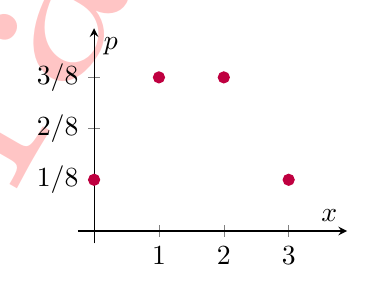
\begin{tikzpicture}
            \begin{axis}[
                width = 5cm,
                xmin = -0.25, xmax = 3.9,
                ymin = -0.03, ymax = 0.495,
                xtick distance = 1,
                ytick = {0.125, 0.25, 0.375},
                yticklabels = {$1/8$, $2/8$, $3/8$},
                ylabel = $p$
            ]
            \draw[purple, fill] (axis cs: 0, 0.125) circle (2pt);
            \draw[purple, fill] (axis cs: 1, 0.375) circle (2pt);
            \draw[purple, fill] (axis cs: 2, 0.375) circle (2pt);
            \draw[purple, fill] (axis cs: 3, 0.125) circle (2pt);
            \end{axis}
        \end{tikzpicture}
    \end{center}
\end{example}

\subsection{Podstawowe rozkłady dyskretne}

Opiszemy teraz pokrótce kilka podstawowych rozkładów zmiennych dyskretnych, pojawiających się stosunkowo często w rozmaitych przykładach i zastosowaniach.
\bigskip

Zmienna $X$ ma \textbf{rozkład dwumianowy} z parametrami $n,p$, oznaczany jako $\purple{X \sim \rpBinom(n,p)}$, jeśli 
$$P(X = k) = \binom{n}{k}p^k(1-p)^{n-k} \qquad \text{dla } k \in \{0,\ldots,n\}$$

Zmienna o rozkładzie dwumianowym opisuje \purple{liczbę sukcesów w schemacie $n$ prób Bernoulliego} o prawdopodobieństwie sukcesu $p$.

\begin{example}
    Rzucamy $n$ razy monetą, na której orzeł wypada z prawdopodobieństwem $p$. Jeśli zmienna $X$ oznacza liczbę orłów w takim ciągu rzutów, to ma ona rozkład dwumianowy:
    $$P(X = k) = \binom{n}{k} p^k (1-p)^{n-k} \qquad \text{dla } k \in \{0,\ldots,n\}$$

    Istotnie, jeśli w ciągu $n$ rzutów wypadło $k$ orłów, to takich różnych ciągów jest $\binom{n}{k}$ \gray{(wybieramy miejsca na orły, a w pozostałych $n - k$ miejscach wrzucamy reszki)}, przy czym każdy z nich mógł przytrafić się z prawdopodobieństwem $p^k (1 - p)^{n - k}$ \gray{($k$ razy wypadł orzeł i $n - k$ razy wypadła reszka)}.
\end{example}

Zmienna $X$ ma \textbf{rozkład geometryczny} z parametrem $p$, oznaczany jako $\purple{X \sim \rpGeom(p)}$, jeśli
$$P(X = k) = (1-p)^{k-1} \cdot p \qquad \text{dla } k \in \NN_+$$

Zmienna o rozkładzie geometrycznym opisuje \purple{numer pierwszej próby zakończonej sukcesem} w nieskończonym schemacie Bernoulliego o prawdopodobieństwie sukcesu $p$.

\begin{example}
    Rzucamy monetą, na której orzeł wypada z prawdopodobieństwem $p$, aż do uzyskania pierwszego orła. Jeśli zmienna $X$ oznacza liczbę rzutów w takim ciągu, to ma ona rozkład geometryczny: 
    $$P(X=k)=(1-p)^{k-1}\cdot p$$

    Istotnie, $X = k$ oznacza, że w $k - 1$ pierwszych rzutach musiała wypaść reszka (z prawdopodobieństwem $1 - p$), a w $k$-tym rzucie wypadł orzeł (z prawdopodobieństwem $p$).
\end{example}

Zmienna $X$ ma \textbf{rozkład Poissona} z parametrem $\lambda$, oznaczany jako $\purple{X \sim \rpPois(\lambda)}$, jeśli
$$P(X = k) = \frac{e^{-\lambda}\lambda^k}{k!} \qquad \text{dla } k \in \NN$$

Rozkład Poissona stosowany jest w rozmaitych kontekstach. Może być stosowany jako dobre przybliżenie rozkładu Bernoulliego $\rpBinom(n, p)$ w przypadku, gdy $n$ jest duże, $p$ jest małe, a $n \cdot p$ wynosi w przybliżeniu $\lambda$. Dzięki temu rozkład Poissona może być używany do badania zdarzeń ,,rzadkich'' i ,,całkowicie losowych'', na przykład:
\begin{itemize}
    \item przewidywanie liczby trzęsień ziemi na podstawie ich średnich wystąpień w przeszłości,
    \item szacowanie liczby błędów ortograficznych w książce o znanej liczbie znaków,
    \item zliczanie liczby telefonów odebranych w centrum obsługi klienta w ciągu godziny.
\end{itemize}

\begin{example}
    Kierownik laboratorium komputerowego otrzymuje średnio $\lambda$ informacji o awarii komputera na miesiąc. Znajdziemy rozkład zmiennej $X$ zliczającej liczbę otrzymanych takich informacji w miesiącu.

    Podzielmy miesiąc na $n$ przedziałów na tyle małych, że otrzymanie dwóch sygnałów w jednym przedziale jest zaniedbywalne (czyli $n\to\infty$). Ponadto, niech zdarzenia odpowiadające otrzymaniu awarii w dwóch różnych przedziałach będą niezależne. Mamy teraz do czynienia z ciągiem $n$ prób Bernoulliego, obliczymy więc prawdopodobieństwo sukcesu (otrzymania informacji o awarii w podanym przedziale).

    Skoro spośród $n$ przedziałów średnio $\lambda$ z niech zawiera awarię, to prawdopodobieństwo wynosi $p = \frac{\lambda}{n}$ i wtedy $X \sim \rpBinom(n,\frac{\lambda}{n})$ dla dużych $n$, czyli
    $$P(X = k) = \binom{n}{k}\left(\frac{\lambda}{n}\right)^k\left(1-\frac{\lambda}{n}\right)^{n-k}$$
    Dla $n \to \infty$ wyrażenie to zbiega do $e^{-\lambda}\lambda^k/k!$, więc (wprost z definicji) $X$ ma rozkład Poissona z parametrem $\lambda$.
\end{example}

\section{Parametry rozkładu}

W tym rozdziale przyjrzymy się kilku istotnym parametrom rozkładów zmiennych losowych, pozwalającym nam na analizowanie ich rozmaitych własności.

\subsection{Wartość oczekiwana}

Niech $X$ będzie zmienną losową o rozkładzie dyskretnym. \textbf{Wartością oczekiwaną} (średnią) $X$ nazywamy wartość sumy
$$
\purple{\E X = \sum_{x\in\RR} \big(x \cdot P(X = x)\big)}
$$

Wartość oczekiwana ma bardzo naturalną fizyczną interpretację: jest to ważona średnia wartości, które mogą być przyjęte przez daną zmienną, gdzie każda wartość ma wagę odpowiadającą jej prawdopodobieństwu.

\begin{example}
    Dysponujemy fałszywą kostką, w której na ścianie z trzema oczkami domalowano dwa dodatkowe oczka. Wyznaczymy wartość oczekiwaną liczby wyrzuconych oczek na tej kostce.

    Oznaczmy odpowiednią zmienną jako $X$. Nietrudno znaleźć jej rozkład:
    $$P(X = k) = \begin{cases}
        1/3 & \text{dla } k = 5 \\
        1/6 & \text{dla } k = 1, 2, 4, 6
    \end{cases}$$

    Szukana przez nas wartość oczekiwana $X$ wynosi więc
    $$\E X = 1 \cdot P(X = 1) + 2 \cdot P(X = 2) + 4 \cdot P(X = 4) + 5 \cdot P(X = 5) + 6 \cdot P(X = 6) =$$ $$= \frac{1}{6}(1 + 2 + 4 + 6) + \frac{1}{3} \cdot 5 = \frac{23}{6}$$
\end{example}

Niekiedy zdarza się, że dysponujemy pewną zmienną losową i interesuje nas nie tyle średnia tej zmiennej, co średnia \textit{pewnej funkcji} tej zmiennej; innymi słowy, mamy zadaną pewną funkcję $f : \RR \to \RR$ i naszym celem jest wyznaczenie $\E f(X)$. Wówczas możemy skorzystać z następującego faktu:
$$\E f(X) = \sum_{x \in \RR} \big(f(x) \cdot P(X = x)\big)$$

\begin{example}
    Losujemy liczbę ze zbioru $\{1, 2, ..., 10\}$. Obliczymy średnią odległość tej liczby od 2.

    Jeśli przez $X$ oznaczymy wylosowaną liczbę, to naszym celem jest obliczenie $\E |X - 2|$. Ponieważ rozkład $X$ to
    $$P(X = j) = 1/10 \qquad \text{dla } j = 1, 2, ..., 10,$$
    na mocy powyższego twierdzenia zachodzi
    $$\E |X - 2| = \sum_{j = 1}^{10} |j - 2| \cdot P(X = j) = \frac{1}{10} \sum_{j = 1}^{10} |j - 2| = \frac{1}{10} + \frac{1}{10} \sum_{j = 3}^{10} |j - 2| = \frac{1}{10} + \frac{36}{10} = 3.7$$
\end{example}

Wartość oczekiwana ma własność \purple{liniowości}, tj. dla dowolnych zmiennych $X, Y$ oraz dowolnego $c \in \RR$ mamy:
\begin{itemize}
    \item $\E (cX) = c \cdot \E X$
    \item $\E (X+Y) = \E X + \E Y$
\end{itemize}

Jeśli $X,Y$ są niezależnymi zmiennymi losowymi (dyskretnymi), to dodatkowo zachodzi \purple{multiplikatywność}: $$\E (XY) = \E X \cdot \E Y$$

\begin{example}
    Rzucono $n$ razy kostką do gry. Obliczymy wartość oczekiwaną łącznej liczby wyrzuconych oczek.

    Oznaczmy szukaną sumę jako $X$. Można próbować obliczyć średnią $X$ bezpośrednio z definicji, ale to bardzo żmudne podejście, gdyż wyznaczenie rozkładu $X$ jest niełatwym zagadnieniem kombinatorycznym.
    
    Aby uniknąć tego problemu, rozbijemy $X$ na sumę prostszych zmiennych: dla $i = 1, 2, ..., n$ przez $X_i$ oznaczymy liczbę oczek wyrzuconych w $i$-tym rzucie. Wówczas $X = X_1 + X_2 + ... + X_n$ oraz 
    $$\E X_i = 1 \cdot P(X_i = 1) + 2 \cdot P(X_i = 2) + ... + 6 \cdot P(X_i = 6) = \frac{7}{2}$$
    i możemy skorzystać z liniowości wartości oczekiwanej:
    $$\E X = \E X_1 + \E X_2 + ... + \E X_n = \frac{7n}{2}$$
\end{example}

\subsection{Wariancja i odchylenie standardowe}

Niech $X$ będzie zmienną losową o skończonej wartości oczekiwanej. \textbf{Wariancję} $X$ definiujemy wzorem
$$\Var X = \E (X - \E X)^2$$

\textbf{Odchyleniem standardowym} zmiennej $X$ nazywamy liczbę $\sigma(X) = \sqrt{\Var X}$.

Przeprowadzając proste przekształcenia, łatwo wyprowadzić alternatywny wzór na wariancję
$$\Var X = \E (X^2) - (\E X)^2,$$
który w wielu sytuacjach oferuje najprostszy sposób jej obliczenia.
\bigskip

O ile wartość oczekiwana mówi nam o tym, jaka jest średnia wartość zmiennej $X$, tak wariancja odpowiada za ,,rozrzut'' jej różnych wartości. Aby lepiej zrozumieć intuicję za tym stojącą, rozważmy trzy zmienne losowe:
\begin{align*}
    X &= 0, \\
    Y & = \begin{cases}
        1 & \text{z prawdopodobieństwem } 1/2, \\
        -1 & \text{z prawdopodobieństwem } 1/2, \\
    \end{cases} \\
    Z & = \begin{cases}
        100 & \text{z prawdopodobieństwem } 1/2, \\
        -100 & \text{z prawdopodobieństwem } 1/2.
    \end{cases}
\end{align*}

Z punktu widzenia wartości oczekiwanej, te zmienne nie różnią się między sobą -- wszystkie mają średnią równą 0. Tym niemniej jest intuicyjnie jasne, że pierwsza z nich nie ma żadnego rozrzutu, druga z nich ma ,,umiarkowany'' rozrzut, a trzecia z nich wykazuje największe odchylenia od swojej wartości oczekiwanej.

Można by się też zastanowić, dlaczego nie definiujemy wariancji bardziej oczywistym (intuicyjnie) wzorem $\E |X - \E X|$, mierzącym wprost jej średnie odchylenie od wartości oczekiwanej? Okazuje się, że tak zdefiniowana wariancja nie jest wygodna -- nie posiada pewnych specjalnych algebraicznych własności. Stąd znacznie lepszym pomysłem jest mierzenie odchylenia w sensie średniokwadratowym $\E (X - \E X)^2$.

\begin{example}
    Ze zbioru $\{1, 2, ..., n\}$ losujemy liczbę $X$. Obliczymy wariancję $X$.

    Rozkład zmiennej $X$ zadany jest przez równości
    $$P(X = k) = 1/n \qquad \text{dla } k = 1, 2, ..., n,$$
    więc
    $$\E X = \sum_{k = 1}^{n} \big(k \cdot P(X = k)\big) = \frac{1}{n} \sum_{k = 1}^{n} k = \frac{n + 1}{2}$$
    i analogicznie
    $$\E (X^2) = \sum_{k = 1}^{n} \big(k^2 \cdot P(X = k)\big) = \frac{1}{n} \sum_{k = 1}^{n} k^2 = \frac{(n + 1)(2n + 1)}{6}$$
    Wobec tego
    $$\Var X = \E (X^2) - (\E X)^2 = \frac{(n + 1)(2n + 1)}{6} - \left(\frac{n + 1}{2}\right)^2 = \frac{n^2 - 1}{12}$$

    Wynika stąd, że dla danego $n$ zmienna $X$ średnio ,,odchyla się'' od swojej wartości oczekiwanej o $\sqrt{\frac{n^2 - 1}{12}}$.
\end{example}

Jeśli zmienne losowe $X$ i $Y$ są niezależne i mają skończoną wariancję, to jest ona \purple{addytywna}:
$$
\Var (X+Y) = \Var X + \Var Y
$$

Ponadto, bezpośrednio z definicji, wariancja posiada następującą własność: jeśli $X$ jest zmienną losową o skończonej wartości oczekiwanej oraz $a, b$ są liczbami rzeczywistymi, to
$$\Var (aX + b) = a^2 \Var X$$

\begin{example}
    Rzucamy trzy razy monetą i przez $X$ oznaczamy różnicę między liczbą wyrzuconych reszek i orłów. Obliczymy wartość oczekiwaną i wariancję $X$.

    Niech $R$ będzie liczbą wyrzuconych reszek, a $O$ -- liczbą orłów. Jasne jest, że $R + O = 3$ oraz $X = R - O$, skąd bezpośrednio wynika, że $X = 2R - 3$. Łatwo wyznaczymy też rozkład $R$:
    $$P(R = 0) = \frac{1}{8}, \qquad P(R = 1) = \frac{3}{8}, \qquad P(R = 2) = \frac{3}{8}, \qquad P(R = 3) = \frac{1}{8}$$

    Wobec tego, korzystając z liniowości wartości oczekiwanej:
    $$\E X = \E (2R - 3) = 2 \E R - \E 3 = 2 \left(0 \cdot \frac{1}{8} + 1 \cdot \frac{3}{8} + 2 \cdot \frac{3}{8} + 3 \cdot \frac{1}{8}\right) - 3 = 0$$
    \gray{(dygresja: wynik ten jest intuicyjnie oczywisty, średnio liczba reszek i orłów jest ta sama i wynosi 1.5)}

    Ponadto, korzystając z podanej wcześniej własności wariancji,
    $$\Var X = \Var (2R - 3) = 4 \Var R$$

    Jak już obliczyliśmy wcześniej, $\E R = 1.5$ oraz
    $$\E R^2 = 0^2 \cdot \frac{1}{8} + 1^2 \cdot \frac{3}{8} + 2^2 \cdot \frac{3}{8} + 3^2 \cdot \frac{1}{8} = 3$$

    Ostatecznie mamy więc
    $$\Var X = 4 \Var R = 4 (\E (R^2) - (\E R)^2) = 3$$
\end{example}

\subsection{Wartości parametrów znanych rozkładów dyskretnych}

Poniższa tabela przedstawia spis wartości oczekiwanych i wariancji dla znanych nam rozkładów dyskretnych. Wszystkie z nich można w łatwy sposób wyprowadzić wprost z definicji, większość powinna również intuicyjnie wynikać z interpretacji kombinatorycznych poszczególnych rozkładów.

\begin{center}
\renewcommand{\arraystretch}{1.5}
\newcolumntype{C}{>{\centering\arraybackslash} m{3cm}}
\begin{tabular}{ C | C | C }
    & $\E X$ & $\Var X$ \\ \hline
    $X \sim \rpBinom(n, p)$ & $np$ & $np(1 - p)$ \\ \hline
    $X \sim \rpGeom(p)$ & $1/p$ & $(1 - p)/p^2$ \\ \hline
    $X \sim \rpPois(\lambda)$ & $\lambda$ & $\lambda$
\end{tabular}
\end{center}

\subsection{Funkcje tworzące prawdopodobieństwa}

Niech $X$ będzie zmienną losową o wartościach naturalnych. \textbf{Funkcją tworzącą prawdopodobieństwa} zmiennej $X$ jest
$$
g_X(t) = \sum_{k=0}^\infty P(X=k)\cdot t^k
$$

Za pomocą funkcji tworzących możemy łatwo obliczać wartość oczekiwaną i wariancję:
$$
\E X = g_X'(1), \qquad \Var X = g_X''(1) + g_X'(1) - g_X'^2(1),
$$
o ile te wartości istnieją i są skończone. Wzory te wynikają wprost z definicji wartości oczekiwanej i wariancji.

\begin{example}
    Znajdziemy funkcję tworzącą prawdopodobieństwa zmiennej $X$ o rozkładzie dwumianowym $\rpBinom(n, p)$.

    Mamy $P(X = k) = \binom{n}{k} p^k (1 - p)^{n - k}$, więc
    $$g_X(t) = \sum_{k = 0}^{n} \binom{n}{k} p^k (1 - p)^{n - k} t^k = \big(pt + (1 - p)\big)^n = (pt - p + 1)^n$$

    Dzięki takiej funkcji łatwo wyprowadzimy wzory na $\E X$ oraz $\Var X$. Zaczniemy od wyznaczenia wzoru na pierwszą i drugą pochodną:
    $$g'_X(t) = np(pt - p + 1)^{n - 1}, \qquad g''_X(t) = n(n - 1)p^2(pt - p + 1)^{n - 2},$$
    skąd otrzymujemy
    $$\E X = g'_X(1) = np, \qquad \Var X = \purple{g_X''(1)} + \teal{g_X'(1)} - \orange{g_X'^2(1)} = \purple{n(n - 1)p^2} + \teal{np} - \orange{n^2p^2} = np - np^2 = np(1 - p)$$
\end{example}

Jeśli $X$ jest zmienną losową o wartościach naturalnych oraz $c$ jest liczbą naturalną, to łatwo możemy wyznaczyć funkcję zmiennej $cX$:
$$g_{cX}(t) = g_X(t^c)$$

Jeśli natomiast $X$ i $Y$ są \purple{niezależnymi} zmiennymi o wartościach naturalnych, to funkcja tworząca prawdopodobieństwa sumy tych zmiennych jest równa
$$g_{X + Y}(t) = g_X(t) \cdot g_Y(t)$$

\begin{example}
    Ponownie obliczymy funkcję tworzącą prawdopodobieństwa dla zmiennej $X$ o rozkładzie dwumianowym $\rpBinom(n, p)$, tym razem rozbijając ją na niezależne zmienne $X_i$ reprezentujące poszczególne próby Bernoulliego w całym schemacie.

    Mamy więc $X = X_1 + X_2 + ... + X_n$, gdzie $P(X_i = 1) = p$ oraz $P(X_i = 0) = 1 - p$. Funkcją tworzącą prawdopodobieństwa dla zmiennych $X_i$ jest
    $$g_{X_i}(t) = P(X_i = 0) t^0 + P(X_i = 1) t^1 = (1 - p) + pt = pt - p + 1,$$
    a skoro $X$ to suma $n$ niezależnych zmiennych o takim rozkładzie, to
    $$g_X(t) = \big(g_{X_i}(t)\big)^n = (pt - p + 1)^n$$
\end{example}

\begin{problems}
    \prob Wrzucamy losowo dwie kule do dwóch urn. Wartość oczekiwana liczby niepustych urn jest równa
    \answers
    {1}
    {$\frac{3}{2}$}
    {$2(1 - \frac{1}{e})$}

    \prob Wrzucamy do worka $n \geq 3$ kul, każdą z nich malujemy niezależnie z prawdopodobieństwem $\frac{1}{2}$ na biało. Wartość oczekiwana liczby białych kul
    \answers{wynosi $\frac{n(n-1)}{2}$}{wynosi $\frac{n}{2}$}{jest większa lub równa wariancji liczby białych kul}

    \prob Dany jest generator bitów, dla którego każdy kolejny wygenerowany bit jest jedynką z prawdopodobieństwem 0.5. Niech $X$ będzie zmienną losową oznaczająca liczbę wygenerowanych jedynek przez ten generator w 100 próbach. Nie wiadomo, czy kolejne losowania są niezależne. Wówczas
    \answers{$\mathrm{E}X = 50$}{$\mathrm{E}X = 50$, gdy kolejne bity są generowane niezależnie}{$\mathrm{Var}(X) = 25$}

    \prob Niech $X$ i $Y$ to zmienne losowe, takie że $\E X = 1$, $\Var X = 4$ i $Y = 2X + 3$. Wtedy
    \answers{$\E Y = 4$}{$\sigma(Y) = 4$}{$\Var Y = 4$}

    \prob Niech $X$ i $Y$ będą zdarzeniami niezależnymi, wtedy
    \answers
    {$\mathrm{E}(X - Y) = \mathrm{E}X - \mathrm{E}Y$}
    {$\mathrm{E}(XY) = \mathrm{E}X \cdot \mathrm{E}Y$}
    {$\mathrm{E}(X / Y) = \mathrm{E}X / \mathrm{E}Y$}

    \prob Niech $X$ i $Y$ będą zmiennymi losowymi o wartościach nieujemnych. Wynika z tego, że
    \answers{$\mathrm{E}(XY)=\mathrm{E}X\cdot \mathrm{E}Y$, jeśli $X$ i $Y$ są niezależne}{$\mathrm{E}(\min(X,Y))=\min(\mathrm{E}X,\mathrm{E}Y)$}{$\mathrm{E}(\min(X,Y))=\min(\mathrm{E}X,\mathrm{E}Y)$, jeśli $X$ i $Y$ są niezależne}
\end{problems}

\section{Nierówności probabilistyczne}

W rachunku prawdopodobieństwa czy statystyce często nie jest możliwe dokładne wyliczenie pewnych interesujących nas wartości. Niemniej jednak, w wielu zastosowaniach istotna jest nie tyle dokładna wartość, co jej oszacowanie.

Przykładowo, gracza może interesować, czy prawdopodobieństwo, że przegra, jest mniejsze niż pewna z góry ustalona liczba i na tej podstawie może podjąć decyzję, czy wziąć udział w grze. Podobnie przy badaniach statystycznych ważne jest oszacowanie prawdopodobieństwa, że błąd wyniesie mniej niż interesująca nas dokładność.

Ogólniej: jeśli przez $X$ oznaczymy losowy błąd danej metody pomiarowej, jesteśmy zainteresowani nierównościami postaci $P(X \geq x) \leq c$, gdzie $c$ jest pewnym ustalonym parametrem.
\bigskip

Podstawowym narzędziem matematycznym służącym do uzyskiwania nierówności powyższego typu jest \textbf{nierówność Markowa}: dla dowolnej nieujemnej zmiennej losowej $X$ oraz dla każdego $c > 0$ zachodzi
$$\purple{P(X \geq c) \leq \frac{\E X}{c}}$$

\begin{example}
    Oszacujemy prawdopodobieństwo uzyskania w 1000 rzutach monetą przynajmniej 750 orłów.
    
    Niech $X_1, X_2, ... ,X_{1000}$ będą wynikami kolejnych rzutów (1 dla orła, 0 dla reszki). Wtedy $X = \sum_{i=1}^{1000} X_i$ jest liczbą wszystkich orłów. Jasne jest też, że $X \sim \rpBinom(1000, \frac{1}{2})$.

    Ponieważ dla rozkładu dwumianowego $\E X = 1000 \cdot \frac{1}{2} = 500$, to z nierówności Markowa otrzymujemy
    $$
    P(X \geq 750) = P\left(X \geq \frac{3}{2} \E X\right) \leq \frac{2}{3}
    $$
    
    Widzimy, że to niezbyt imponujące oszacowanie (intuicyjnie wynik powinien być dużo niższy).
\end{example}

Nierówność Markowa, choć niezwykle prosta, ma bardzo dużo zastosowań. Jej siła wynika między innymi z faktu, że możemy zastosować ją nie tylko do zmiennej losowej $X$, którą jesteśmy zainteresowani, ale także do zmiennych postaci $f(X)$, uzyskując nowe nierówności.

Na przykład, podstawiając zmienną $(X - \E X)^2$ do nierówności Markowa, uzyskamy \textbf{nierówność Czebyszewa}: dla dowolnej nieujemnej losowej $X$ oraz dla każdego $c > 0$ zachodzi
$$
\purple{P(|X - \E X| \geq c) \leq \frac{\Var X}{c^2}}
$$

\begin{example}
    Kontynuujemy poprzedni przykład. Tym razem oszacujemy prawdopodobieństwo uzyskania co najmniej 750 orłów w ciągu 1000 rzutów monetą za pomocą nierówności Czebyszewa.

    Dla zmiennej $X$ o rozkładzie dwumianowym mamy $\E X = 1000 \cdot \frac{1}{2} = 500$ oraz $\Var X = 1000 \cdot \frac{1}{2} \cdot (1 - \frac{1}{2}) = 250$.
    
    Nierówność Czebyszewa pozwoli nam na oszacowanie prawdopodobieństwa $P(|X - 500| \geq c)$ dla pewnej ustalonej liczby $c \in \RR$. Aby móc otrzymać z tego $P(X \geq 750)$, skorzystamy z faktu, że w schemacie Bernoulliego (u nas: 1000 rzutów monetą) zachodzi symetria $P(X \geq 750) = P(X \leq 250)$, co pozwala nam uzyskać równość
    $$P(|X - 500| \geq 250) = P(X \geq 750) + P(X \leq 250) = 2 \cdot P(X \geq 750),$$
    więc mamy
    $$
    P(X \geq 750) = \frac{1}{2} \cdot P(|X - 500| \geq 250) \leq \frac{1}{2} \cdot \frac{250}{250^2} = \frac{1}{500}
    $$
    
    Widzimy, że to dużo lepsze oszacowanie niż poprzednio.
\end{example}

% TODO
\begin{editorsnote}
    W rozdziale brakuje informacji na temat nierówności Chernoffa (jest ona wspomniana w podstawie programowej), jednak zawarta tu teoria jest wystarczająca do rozwiązania zadań z przeanalizowanych na potrzeby tego repetytorium archiwalnych egzaminów.
\end{editorsnote}

\begin{problems}
    \prob Niech $X$ będzie zmienną losową reprezentującą długość trwania programu dla różnych wejść, niech $\mu$ to wartość oczekiwana $X$, zaś $\sigma$ to odchylenie standardowe. Prawdą jest, że
    \answers{$P(X > 2\mu) \leq \frac{1}{4}$}{$P(X > \mu + 2\sigma) \leq \frac{1}{4}$}{$P(X > 100\mu) \leq \frac{1}{10^{10}}$}
\end{problems}

\section{Ciągły rozkład prawdopodobieństwa}

Dla dyskretnych zmiennych losowych mieliśmy $\sum_{x \in \RR} P(X = x) = 1$, czyli suma prawdopodobieństw przeliczalnie wielu wartości uzyskiwanych przez zmienną jest równa 1. Zauważmy jednak, że taka zmienna nie pozwoliłaby nam rozpatrzeć doświadczenia polegającego na wylosowaniu punktu z odcinka $[0, 1]$ -- ponieważ zbiór ten jest nieprzeliczalny, a każdy punkt równo prawdopodobny do wylosowania, nie potrafilibyśmy określić prawdopodobieństwa wylosowania pojedynczego punktu, tak żeby wszystkie z nich zsumowały się do 1.

Podobnie jest w każdej sytuacji, w której wynikiem jakiegoś doświadczenia może być dowolna liczba rzeczywista, np. pomiar wzrostu osoby lub prędkości samochodu. Mamy tu do czynienia z \textbf{ciągłym rozkładem prawdopodobieństwa} i w tym rozdziale zobaczymy, jak sobie z nim poradzić.

\subsection{Prawdopodobieństwo geometryczne}

O ile w problemach dyskretnych korzystamy zazwyczaj ze schematu klasycznego, tak w doświadczeniach losowych o charakterze ciągłym przydatne może okazać się \textbf{prawdopodobieństwo geometryczne}. Najprostszym przykładem jest losowanie punktu z pewnego zbioru $\Omega$.

Załóżmy, że $\Omega$ jest pewnym podzbiorem przestrzeni $\RR^d$ i ma skończoną miarę (długość, pole powierzchni, objętość... -- w zależności od wymiaru $d$). Wówczas prawdopodobieństwo dowolnego zdarzenia $A \subseteq \Omega$ jest \purple{proporcjonalne do jego miary}:
$$P(A) = \frac{|A|}{|\Omega|}$$

\begin{example}
    Z przedziału $[0, 1]$ wybieramy losowo dwie liczby. Jakie jest prawdopodobieństwo tego, że obie te liczby są mniejsze niż $1/2$?

    Zastosujemy prawdopodobieństwo geometryczne. Oznaczmy wybrane liczby przez $x, y$. Wówczas
    $$\Omega = \{(x, y) \ | \ x, y \in [0, 1]\} = [0, 1]^2$$

    Następnym krokiem jest zinterpretowanie badanego zdarzenia $A$ jako podzbioru $\Omega$. Mamy
    $$A = \left\{(x, y) \in \Omega \ | \ x, y \leq \frac{1}{2}\right\} = \left[0, \frac{1}{2}\right]^2,$$
    a zatem obliczając pola powierzchni odpowiednich zbiorów:
    $$P(A) = \frac{|A|}{|\Omega|} = \frac{1}{4}$$

    Możemy to łatwo zwizualizować w układzie współrzędnych:
    \begin{center}
        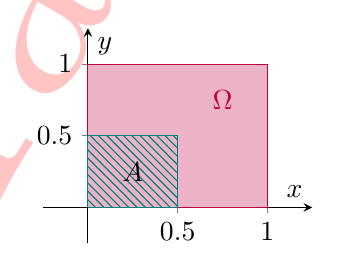
\begin{tikzpicture}
            \begin{axis}[
                width = 5 cm,
                xmin = -0.25, xmax = 1.25,
                ymin = -0.25, ymax = 1.25,
                xtick distance = 0.5,
                ytick distance = 0.5,
            ]
                \addplot [
                    draw=purple,
                    fill=purple,
                    fill opacity=0.3,
                ] coordinates {(0, 0) (1, 0) (1, 1) (0, 1) (0, 0)};
                
                \addplot [
                    draw=teal,
                    pattern=north west lines,
                    pattern color=teal,
                ] coordinates {(0, 0) (0.5, 0) (0.5, 0.5) (0, 0.5) (0, 0)};
                
                \node at (axis cs: 0.75, 0.75) {\textcolor{purple}{$\Omega$}};
                \node at (axis cs: 0.25, 0.25) {$A$};
            \end{axis}
        \end{tikzpicture}
    \end{center}
\end{example}

\subsection{Ciągłe zmienne losowe}

Zmienna $X$ ma \textbf{rozkład ciągły}, jeśli istnieje funkcja $f_X : \RR \to \RR_{\geq0}$, taka że dla każdego przedziału $[a, b]$ zachodzi
$$P(X \in [a, b]) = \int_a^b f_X(x) \dx$$

Funkcja $f_X$ w powyższej definicji to \textbf{funkcja gęstości} zmiennej $X$. Dla zmiennej ciągłej prawdopodobieństwo, że zmienna przyjmie wartość między $a$ i $b$ jest równe polu powierzchni pod krzywą gęstości nad tym odcinkiem:

\begin{center}
    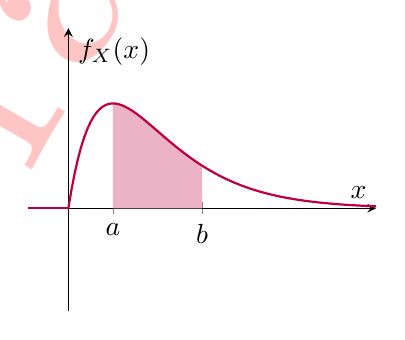
\begin{tikzpicture}
        \begin{axis}[
            width = 6cm,
            xmin = -0.9, xmax = 6.9,
            ymin = -0.4, ymax = 0.7,
            xtick = {1, 3},
            xticklabels = {$a$, $b$},
            ylabel = $f_X(x)$,
            ytick distance = 1,
            samples = 100
        ]
            \addplot[thick, purple, domain = -1:0] {0};
            \addplot[draw = none, fill = purple!30, domain = 1:3] {0.15 * x * e^(-(x-2))} \closedcycle;
            \addplot[thick, purple, domain = 0:7] {0.15 * x * e^(-(x-2))};
        \end{axis}
    \end{tikzpicture}
\end{center}

Oczywiste jest również, że prawdopodobieństwa wszystkich możliwych wartości $X$ muszą sumować się do 1, w związku z czym dla każdej funkcji gęstości mamy
$$\int_{-\infty}^{+\infty} f_X(x) \dx = 1$$

\begin{example}
    Rzucamy niesymetryczną monetą, na której prawdopodobieństwo wypadnięcia orła wynosi 1/3. Jeśli wypadnie orzeł, to losujemy punkt $X$ z odcinka $[-2, 0)$, a jeśli wypadnie reszka, to losujemy $X$ z odcinka $[0, 3]$. Wyznaczymy funkcję gęstości zmiennej $X$.

    Żeby $X$ przyjęło jedną z wartości z przedziału $[-2, 0)$, na monecie musi wypaść orzeł (z prawdopodobieństwem 1/3). Ponieważ wylosowanie każdego punktu jest równie prawdopodobne, dla $x \in [-2, 0)$ mamy
    $$f_X(x) = \frac{1}{3} \cdot \frac{1}{0 - (-2)} = \frac{1}{6}$$

    Analogicznym rozumowaniem dla reszki i przedziału $[0, 3]$ dochodzimy do wniosku, że funkcją gęstości zmiennej $X$ jest
    $$
    f_X(x) = \begin{cases}
        \frac{1}{6} & \text{dla } x \in [-2, 0), \\
        \frac{2}{9} & \text{dla } x \in [0, 3], \\
        0 & \text{wpp.}
    \end{cases}
    $$

    Oznacza to, że $X$ przyjmie wartość z przedziału $[-2, 0)$ z prawdopodobieństwem 1/6 oraz wartość z przedziału $[0, 3]$ z prawdopodobieństwem 2/9. Możemy zobrazować $f_X$ w układzie współrzędnych:
    \begin{center}
        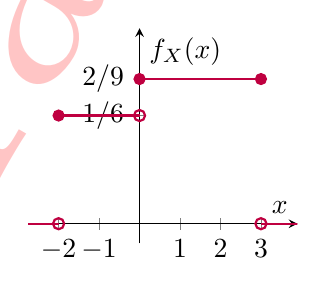
\begin{tikzpicture}
            \begin{axis}[
                width = 5cm,
                xmin = -2.75, xmax = 3.9,
                ymin = -0.03, ymax = 0.3,
                xtick distance = 1,
                ylabel = $f_X(x)$,
                ytick = {0.166, 0.222},
                yticklabels = {$1/6$, $2/9$}
            ]
            \addplot[thick, purple, domain = -3:-2] {0};
            \addplot[thick, purple, domain = -2:0] {0.166};
            \addplot[thick, purple, domain = 0:3] {0.222};
            \addplot[thick, purple, domain = 3:4] {0};
            \draw[purple, thick] (axis cs: -2, 0) circle (2pt);
            \draw[purple, fill] (axis cs: -2, 0.166) circle (2pt);
            \draw[purple, thick] (axis cs: 0, 0.166) circle (2pt);
            \draw[purple, fill] (axis cs: 0, 0.222) circle (2pt);
            \draw[purple, fill] (axis cs: 3, 0.222) circle (2pt);
            \draw[purple, thick] (axis cs: 3, 0) circle (2pt);
            \end{axis}
        \end{tikzpicture}
    \end{center}

    Z rysunku nietrudno przekonać się też, że
    $$\int_{-\infty}^{\infty} f_X(x) = 2 \cdot \frac{1}{6} + 3 \cdot \frac{2}{9} = 1,$$
    co potwierdza dobre zdefiniowanie funkcji gęstości.
\end{example}

Znany jest jeszcze jeden ważny fakt dotyczący rozkładu sum niezależnych zmiennych losowych o rozkładzie ciągłym.

Załóżmy, że $X, Y$ są \purple{niezależnymi} ciągłymi zmiennymi losowymi z gęstościami $f_X, f_Y$. Wówczas zmienna $X + Y$ ma rozkład z gęstością będącą splotem funkcji $f_X$ i $f_Y$:
$$f_{X + Y}(x) = \int_{-\infty}^{+\infty} f_X(y) f_Y(x - y) \dy$$

\subsection{Dystrybuanta}

W przypadku doświadczeń losowych o charakterze ciągłym z reguły jesteśmy zainteresowani zdarzeniami typu $P(X \leq c)$ dla pewnej zmiennej losowej $X$ i liczby rzeczywistej $c$.

\textbf{Dystrybuanta} zmiennej losowej $X$ to funkcja $F_X : \RR \to [0, 1]$ określona jako $$F_X(x) = P(X \leq x)$$

Nietrudno zauważyć, że dystrybuanta jest ściśle powiązana z funkcją gęstości, przez co \purple{jednoznacznie determinuje rozkład} dowolnej zmiennej losowej.

Co ważne: dystrybuanta nie jest związana wyłącznie z pojęciem rozkładu ciągłego i może być stosowana także do innych zmiennych.

\begin{example}
    Rozważmy (dyskretną) zmienną losową dwupunktową, przyjmującą wartości $1$ i $-1$, każdą z prawdopodobieństwem 1/2. Jej dystrybuantą jest funkcja
    $$F(x) = \begin{cases}
        0 & \text{dla } x \in (-\infty, -1), \\
        \frac{1}{2} & \text{dla } x \in [-1, 1), \\
        1 & \text{dla } x \in [1, \infty).
    \end{cases}$$
\end{example}

Możemy zauważyć, że nie każda funkcja może być dystrybuantą -- ma to związek ze znanymi nam podstawowymi własnościami prawdopodobieństwa. W szczególności wyróżniamy następujące \purple{własności dystrybuanty}:
\begin{enumerate}
    \item $F_X$ jest niemalejąca,
    \item $F_X$ jest prawostronnie ciągła,
    \item $\Lim_{x \to -\infty} F_X(x) = 0$ oraz $\Lim_{x \to +\infty} F_X(x) = 1$.
\end{enumerate}

Dodatkowo, \purple{jeśli $X$ jest zmienną ciągłą, to $F_X$ jest funkcją ciągłą}.
\bigskip

Intuicyjnie patrząc na definicje dystrybuanty i funkcji gęstości można dojść do wniosku, że ich wzajemne powiązanie wygląda podobnie jak relacja funkcji i jej pochodnej. Istotnie, istnieje twierdzenie, które w wielu sytuacjach pozwala obliczyć gęstość zmiennej losowej, gdy znana jest jej dystrybuanta:

Niech $X$ będzie ciągłą zmienną losową. Wtedy jej dystrybuanta $F_X$ jest różniczkowalna wszędzie poza skończonym zbiorem punktów oraz funkcja
$$
f_X(x) = \begin{cases}
    F_X'(x) & \text{jeśli } F_X'(x) \text{ istnieje,} \\
    0 & \text{wpp.}
\end{cases}
$$
jest gęstością zmiennej $X$.

\begin{example}
    Rozważmy zmienną losową $X$ o dystrybuancie
    $$
    F_X(x) = \begin{cases}
        0 & \text{dla } x \in (-\infty, 0), \\
        2x & \text{dla } x \in (0, \frac{1}{2}), \\
        1 & \text{dla } x \in (\frac{1}{2}, \infty).
    \end{cases}
    $$

    Funkcja $F_X$ jest różniczkowalna wszędzie poza punktami $x = 0$ i $x = 1/2$. Ponadto, $F_X'(x) = 0$ dla $x \in (-\infty, 0) \cup (1/2, \infty)$ oraz $F_X'(x) = 2$ dla $x \in (0, 1/2)$. Zatem funkcja
    $$
    f_X(x) = \begin{cases}
        0 & \text{dla } x \in (-\infty, 0] \cup [\frac{1}{2}, \infty), \\ 
        2 & \text{dla } x \in (0, \frac{1}{2}).
    \end{cases}
    $$
    jest gęstością zmiennej $X$.
\end{example}

Warto również na tym etapie podkreślić, że \purple{istnieją rozkłady, które nie są ani ciągłe, ani dyskretne}, co obrazuje poniższy przykład.

\begin{example}
    Rzucamy standardową monetą i jeśli wypadnie orzeł, to zmienna $X$ przyjmuje wartość 3, a jeśli reszka, zmienna $X$ ma wartość wylosowaną z przedziału $(0, 1)$.

    Dystrybuanta takiego rozkładu to
    $$
    F_X(x) = \begin{cases}
        0 & \text{dla } x \in (-\infty, 0), \\
        \frac{x}{2} & \text{dla } x \in [0, 1), \\
        \frac{1}{2} & \text{dla } x \in [1, 3), \\
        1 & \text{dla } x \in [3, \infty), \\
    \end{cases}
    $$

    Zmienna $X$ nie jest więc ani dyskretna (może przyjąć nieprzeliczalnie wiele wartości), ani ciągła (jej dystrybuanta nie jest ciągła w punkcie $x = 3$).
\end{example}

\subsection{Podstawowe rozkłady ciągłe}

Opiszemy teraz pokrótce kilka podstawowych rozkładów zmiennych ciągłych, pojawiających się stosunkowo często w rozmaitych przykładach i zastosowaniach.
\bigskip

Zmienna $X$ ma \textbf{rozkład jednostajny} z parametrami $a, b$, oznaczany jako $\purple{X \sim \rpUnif(a, b)}$, jeśli $X$ ma gęstość 
$$f_X(x) = \frac{1}{b - a} \qquad \text{dla } x \in [a, b]$$

Zmienna o rozkładzie jednostajnym opisuje \purple{losowanie liczby z zakresu $[a, b]$} o równo rozłożonym prawdopodobieństwie.

\begin{center}
    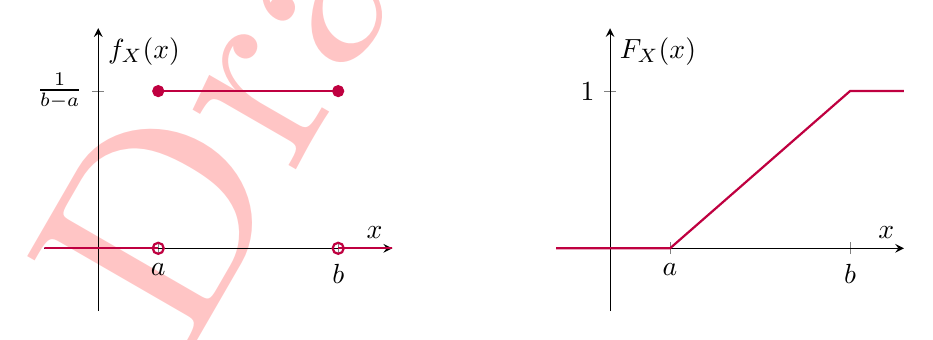
\begin{tikzpicture}
        \begin{axis}[
            width = 6cm,
            xmin = -0.9, xmax = 4.9,
            ymin = -0.4, ymax = 1.4,
            xtick = {1, 4},
            xticklabels = {$a$, $b$},
            ylabel = $f_X(x)$,
            ytick = {1},
            yticklabels = {$\frac{1}{b - a}$}
        ]
            \addplot[thick, purple, domain = -1:1] {0};
            \addplot[thick, purple, domain = 1:4] {1};
            \addplot[thick, purple, domain = 4:5] {0};
            \draw[purple, thick] (axis cs: 1, 0) circle (2pt);
            \draw[purple, fill] (axis cs: 1, 1) circle (2pt);
            \draw[purple, fill] (axis cs: 4, 1) circle (2pt);
            \draw[purple, thick] (axis cs: 4, 0) circle (2pt);
        \end{axis}
        
        \begin{axis}[
            width = 6cm,
            xmin = -0.9, xmax = 4.9,
            ymin = -0.4, ymax = 1.4,
            xtick = {1, 4},
            xticklabels = {$a$, $b$},
            ylabel = $F_X(x)$,
            ytick = {1},
            at = {(6.5cm, 0)}
        ]
            \draw[purple, thick] (axis cs: -1, 0) -- (axis cs: 1, 0) -- (axis cs: 4, 1) -- (axis cs: 5, 1);
        \end{axis}
    \end{tikzpicture}
\end{center}
\bigskip

Zmienna $X$ ma \textbf{rozkład wykładniczy} z parametrem $\theta$, oznaczany jako $\purple{X \sim \rpExp(\theta)}$, jeśli $X$ ma gęstość 
$$f_X(x) = \theta e^{-\theta x} \qquad \text{dla } x \geq 0$$

Zmienna o rozkładzie wykładniczym modeluje \purple{czas oczekiwania na zdarzenie, które ma cały czas taką samą szansę zajścia}, na przykład telefon w centrum telefonicznym lub czas do zajścia rozpadu radioaktywnego. Parametr $\theta$ określa średnią liczbę wystąpień badanego zdarzenia w ustalonej jednostce czasu. O rozkładzie tym można myśleć jak o \purple{ciągłej wersji rozkładu geometrycznego}.

\begin{center}
    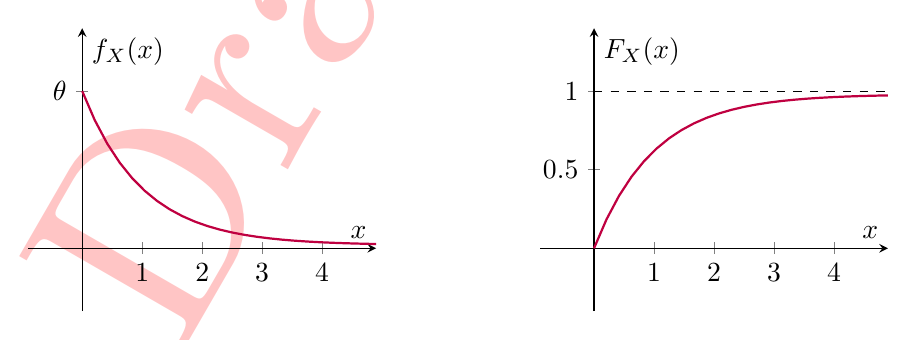
\begin{tikzpicture}
        \begin{axis}[
            width = 6cm,
            xmin = -0.9, xmax = 4.9,
            ymin = -0.4, ymax = 1.4,
            xtick distance = 1,
            ylabel = $f_X(x)$,
            ytick = {1},
            yticklabels = {$\theta$}
        ]
            \addplot[thick, purple, domain = 0:5] {0.02 + (0.98 * e^(-x))};
        \end{axis}
        
        \begin{axis}[
            width = 6cm,
            xmin = -0.9, xmax = 4.9,
            ymin = -0.4, ymax = 1.4,
            xtick distance = 1,
            ylabel = $F_X(x)$,
            ytick distance = 0.5,
            at = {(6.5cm, 0)}
        ]
            \addplot[thick, purple, domain = 0:5] {0.98 * (1 - e^(-x))};
            \draw[dashed] (axis cs: 0, 1) -- (axis cs: 5, 1);
        \end{axis}
    \end{tikzpicture}
\end{center}
\bigskip

Zmienna $X$ ma \textbf{rozkład normalny} (Gaussa) o wartości oczekiwanej $\mu$ i odchyleniu standardowym $\sigma$, oznaczany jako $\purple{X \sim \rpN(\mu, \sigma)}$, jeśli $X$ ma gęstość 
$$f_X(x) = \frac{1}{\sqrt{2\pi} \sigma} e^{-\frac{(x - \mu)^2}{2\sigma^2}}$$

Rozkład normalny ma dość skomplikowaną definicję. Suma dużej liczby niezależnych zmiennych, z których żadna nie dominuje pozostałych (tj. nie przyjmuje dużo większych wartości ani nie ma decydującego wpływu wynik) ma w przybliżeniu rozkład normalny. Przykładem może być wzrost lub masa człowieka o zbliżonych cechach, np. płci i rasie.

Rozkład $\rpN(0, 1)$ nazywamy \textbf{standardowym rozkładem normalnym}. Często pojawia się on w definicjach innych rozkładów oraz różnych rozumowaniach.

\begin{center}
    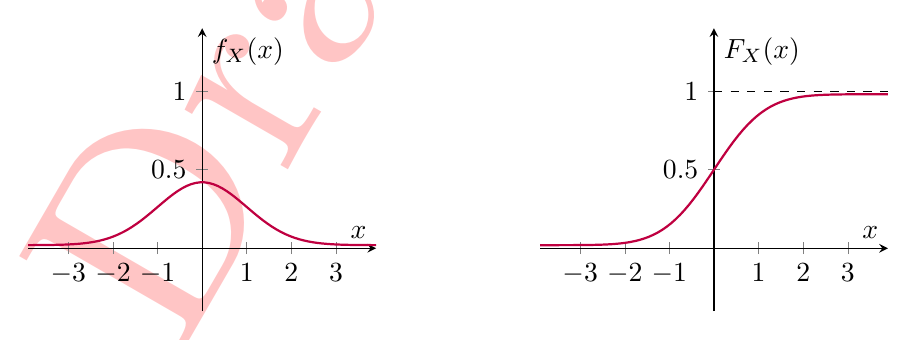
\begin{tikzpicture}
        \begin{axis}[
            width = 6cm,
            xmin = -3.9, xmax = 3.9,
            ymin = -0.4, ymax = 1.4,
            xtick distance = 1,
            ylabel = $f_X(x)$,
            ytick distance = 0.5,
            samples = 100
        ]
            \addplot[thick, purple] {0.02 + (0.4 * e^(-0.5 * x^2))};
        \end{axis}
        
        \begin{axis}[
            width = 6cm,
            xmin = -3.9, xmax = 3.9,
            ymin = -0.4, ymax = 1.4,
            xtick distance = 1,
            ylabel = $F_X(x)$,
            ytick distance = 0.5,
            samples = 100,
            at = {(6.5cm, 0)}
        ]
            \addplot[thick, purple] {0.02 + (0.48 * (1 + tanh(sqrt(pi)/2 * (x + 0.044715 * x^3))))};
            \draw[dashed] (axis cs: 0, 1) -- (axis cs: 5, 1);
        \end{axis}
    \end{tikzpicture}
\end{center}

Jeśli $X, Y$ są \purple{niezależnymi} zmiennymi losowymi o rozkładzie normalnym ze średnimi $\mu_X, \mu_Y$ oraz odchyleniami standardowymi $\sigma_X, \sigma_Y$, to
\begin{itemize}
    \item zmienna losowa $X + Y$ ma rozkład normalny $\rpN(\mu_X + \mu_Y, \sqrt{\sigma_X^2 + \sigma_Y^2})$,
    \item zmienna losowa $X - Y$ ma rozkład normalny $\rpN(\mu_X - \mu_Y, \sqrt{\sigma_X^2 + \sigma_Y^2})$.
\end{itemize}

\subsection{Parametry rozkładów ciągłych}

W ogólności \purple{wszystkie podstawowe własności wartości oczekiwanej i wariancji przenoszą się z przypadku dyskretnego na ciągły}. Dla formalności, poniżej uogólnimy jedynie podstawowe definicje.
\bigskip

Niech $X$ będzie ciągłą zmienną losową o gęstości $f_X$. \textbf{Wartością oczekiwaną} $X$ nazywamy wartość
$$\E X = \int_{-\infty}^{+\infty} x f_X(x) \dx,$$
o ile $|x|f_X(x)$ jest całkowalna. Jeśli wartość oczekiwana istnieje, to \textbf{wariancję} obliczamy ze standardowego wzoru:
$$\Var X = \E(X - \E X)^2 \textqq{albo} \Var X = \E(X^2) - (\E X)^2$$

\subsection{Wartości parametrów znanych rozkładów ciągłych}

Poniższa tabela przedstawia spis wartości oczekiwanych i wariancji dla znanych nam rozkładów ciągłych.

\begin{center}
\renewcommand{\arraystretch}{1.5}
\newcolumntype{C}{>{\centering\arraybackslash} m{3cm}}
\begin{tabular}{ C | C | C }
    & $\E X$ & $\Var X$ \\ \hline
    $X \sim \rpUnif(a, b)$ & $(a + b)/2$ & $(a - b)^2 / 12$ \\ \hline
    $X \sim \rpExp(\theta)$ & $1/\theta$ & $1/\theta^2$ \\ \hline
    $X \sim \rpN(\mu, \sigma)$ & $\mu$ & $\sigma$
\end{tabular}
\end{center}

\subsection{Centralne twierdzenie graniczne}

Rozkłady normalne należą do najważniejszych rozkładów w rachunku prawdopodobieństwa. Okazuje się, że wiele występujących w przyrodzie wielkości ma rozkład w przybliżeniu normalny, np. rozkład wzrostu, wagi, ilorazu inteligencji czy innych cech populacji. Matematyczne wyjaśnienie tego faktu opisuje \textbf{centralne twierdzenie graniczne}.
\bigskip

Niech $X_1, X_2 ...$ będzie ciągiem niezależnych zmiennych losowych o tym samym rozkładzie, wartości oczekiwanej $\mu$ i wariancji $\sigma^2 > 0$. Wówczas dla dowolnego $t \in \RR$ mamy
$$
\limn P\left(\frac{X_1 + X_2 + ... + X_n - n \mu}{\sigma \sqrt{n}} \leq t\right) = \Phi(t),
$$
gdzie $\Phi$ to dystrybuanta standardowego rozkładu normalnego $N(0,1)$. Jej konkretne wartości można znaleźć w tablicach matematycznych.

Twierdzenie to mówi, że rozkład sumy wielu niezależnych zmiennych o tym samym rozkładzie jest bliski normalnemu.

\begin{example}
    Rzucono monetą 10000 razy i okazało się, że orzeł wypadł 5200 razy. Sprawdzimy, jak duże są podstawy do przypuszczenia, że moneta jest niesymetryczna.

    Rozważmy ciąg zmiennych $X_i$ przyjmujących wartość 1, jeśli w $i$-tym rzucie wypadł orzeł, lub wartość 0 w przeciwnym przypadku. Jasne jest, że $X_1, X_2, ..., X_{10000}$ są niezależne o tym samym rozkładzie, możemy więc zastosować centralne twierdzenie graniczne, żeby oszacować prawdopodobieństwo rozważanego zdarzenia (5200 orłów w ciągu 10000 rzutów).

    Łatwo obliczamy $\E X_i = 1/2$ oraz $\Var X_i = 1/4$, stąd $\mu = 1/2$ i $\sigma = \sqrt{\Var X_i} = 1/2$ i dalej
    $$P(X_1 + X_2 + ... + X_{10000} \leq 5200) = P(X_1 + X_2 + ... + X_{10000} - 10000\mu \leq 5200 - 5000) =$$
    $$= P\left(\frac{X_1 + X_2 + ... + X_{10000} - 10000 \mu}{\sigma \sqrt{10000}} \leq \frac{200}{50}\right) \approx \Phi(4)$$

    Sprawdzając w tablicach: $\Phi(4) \approx 0.99997$, więc prawdopodobieństwo, że $X_1 + X_2 + ... + X_{10000} \geq 5200$ (zdarzenie przeciwne do obliczonego powyżej -- w 10000 rzutach monetą wyrzucimy przynajmniej 5200 orłów) ma prawdopodobieństwo $1 - \Phi(4) \approx 0.00003$. To bardzo mało; są więc podstawy, by sądzić, że moneta nie jest symetryczna.
\end{example}

\begin{problems}
    \prob Zmienne $X$ i $Y$ mają rozkład jednostajny na przedziale $[0, 2]$. Jeśli $Z = X + Y$, to
    \answers{$P(Z \geq 1) = \frac{7}{8}$}{$Z$ ma rozkład jednostajny na $[0, 4]$ i wartość oczekiwaną 2}{$P(|\mathrm{E}Z - Z| \geq 1) > \frac{2}{3}$}

    \prob Niech $F_{X}(t)$ będzie dystrybuantą pewnej zmiennej losowej $X$. Załóżmy, że $F_{X}(1)=\frac{1}{3}$. Wynika z tego, że
    \answers{istnieje takie $t$, że $F_{X}(t) = 1$}{$F_X(2) > \frac{1}{3}$}{istnieje takie $t$, że $F_{X}(t) < \frac{1}{4}$}

    \prob Niech $X$ i $Y$ będą niezależnymi zmiennymi losowymi. Wynika z tego, że
    \answers{jeśli $X$ i $Y$ mają rozkład Poissona, to $X - Y$ też}{jeśli $X$ i $Y$ mają rozkład normalny, to $X - Y$ też}{jeśli $X$ i $Y$ mają rozkład geometryczny, to $X - Y$ też}

    \prob Niech $X$ i $Y$ będą dwiema niezależnymi zmiennymi losowymi o rozkładzie normalnym o wartości oczekiwanej 0 i wariancji 4. Wynika z tego, że
    \answers
    {$X - Y$ ma taki sam rozkład jak $X + Y$}
    {odchylenie standardowe zmiennej losowej $X - Y$ jest równe 4}
    {dla $a, b > 0$ zmienna losowa $aX + bY$ ma rozkład normalny}
\end{problems}

\section{Łańcuchy Markowa}

% TODO
\begin{editorsnote}
    Rozdział nie jest jeszcze stworzony -- w historii przeanalizowanych na potrzeby tego repetytorium egzaminów nie pojawiło się żadne zadanie z łańcuchów Markowa.
\end{editorsnote}

\begin{solutions}
    % Kasia K
    \sol Istnieje przestrzeń probabilistyczna $\Omega$ i zdarzenia $A,B\subseteq\Omega$ takie, że $P(A)=P(B)=\frac{2}{3}$ oraz
    \answerss{$A$ i $B$ są niezależne}{$P(A|B)=\frac{1}{3}$}{$P(A|B)\neq P(B|A)$}{TAK}{NIE}{NIE}

    Przy rozwiązaniu tego typu zadań dobrze skorzystać z diagramu Venna. Łatwo można zauważyć, że zachodzi $\frac{1}{3} \leq P(A \cap B) \leq \frac{2}{3}$, a to pomoże w dalszych rozważaniach:
    \begin{enumerate}[\bf A.]
        \item Żeby $A$ i $B$ były niezależne, musi zachodzić
        $$P(A \cap B) = P(A) \cdot P(B) = \frac{4}{9}$$
        Ponieważ $\frac{1}{3} \leq \frac{4}{9} \leq \frac{2}{3}$, taka sytuacja jest możliwa.
        
        \item Tym razem mamy
        $$P(A | B) = \frac{P(A \cap B)}{P(B)} \wtw P(A \cap B) = P(A|B) \cdot P(B) = \frac{1}{3} \cdot \frac{2}{3} = \frac{2}{9}$$
        Ponieważ $\frac{2}{9} < \frac{1}{3}$, taka sytuacja nie może zajść.
        
        \item Zauważmy, że dla dowolnych zdarzeń $A, B$ spełniających warunki zadania jest
        $$P(A|B) = \frac{P(A \cap B)}{P(B)} = \frac{P(A \cap B)}{2/3} = \frac{P(A \cap B)}{P(A)} = P(B|A)$$
    \end{enumerate}

    %Tomek
    \sol Chcemy rozpalić ognisko, lecz mamy do dyspozycji tylko trzy zapałki. Prawdopodobieństwo rozpalenia ogniska pojedynczą zapałką wynosi $0.4$, dwiema złączonymi zapałkami -- $0.6$, zaś trzema złączonymi zapałkami -- $0.8$. Żeby zmaksymalizować prawdopodobieństwo rozpalenia ogniska, należy
    \answerss
    {użyć od razu trzech zapałek}
    {użyć najpierw dwóch zapałek, a potem jednej}
    {używać pojedynczych zapałek}
    {TAK}{NIE}{NIE}

    Oznaczmy zdarzenia:
    \begin{itemize}
        \item $A$ -- rozpalimy ognisko trzema złączonymi zapałkami,
        \item $B$ -- rozpalimy ognisko dwiema zapałkami, a potem jedną,
        \item $C$ -- rozpalimy ognisko trzema pojedynczymi zapałkami.
    \end{itemize}

    Obliczamy i porównujemy poszczególne prawdopodobieństwa:
    \begin{itemize}
        \item $P(A) = 0.8$
        \item $P(B) = 0.6 + (1 - 0.6) \cdot 0.4 = 0.76$ \gray{(odpalamy za pierwszym razem dwoma zapałkami lub nie odpalamy za pierwszym razem i odpalamy za drugim)}
        \item $P(C) = 0.4 + (1 - 0.4) \cdot 0.4 + (1 - 0.4)^2 \cdot 0.4 = 0.784$ \gray{(analogiczne rozumowanie -- rozpalamy za pierwszym, drugim albo trzecim razem)}
    \end{itemize}

    Najbardziej opłacalne jest więc użycie trzech złączonych zapałek.

    \sol Rzucamy 10 razy symetryczną monetą. Wynika z tego, że
    \answerss
    {prawdopodobieństwo, że wyrzucimy dokładnie 2 orły jest równe $\frac{45}{1024}$}
    {prawdopodobieństwo, że wyrzucimy orła w ostatnim rzucie pod warunkiem, że we wszystkich 10 rzutach wyrzucimy dokładnie 1 orła, jest równe $\frac{1}{2}$}
    {prawdopodobieństwo, że wyrzucimy orła w ostatnim rzucie pod warunkiem, że w pierwszych 9 rzutach wyrzucimy dokładnie 6 orłów, jest równe $\frac{1}{2}$}
    {TAK}{NIE}{NIE}

    \begin{enumerate}[\bf A.]
        \item Oznaczmy zdarzenie ,,wyrzucono dokładnie 2 orły'' jako $A$. W zadaniu mamy do czynienia ze schematem 10 prób Bernoulliego o prawdopodobieństwie sukcesu $\frac{1}{2}$ (wyrzucono orła). W związku z tym
        $$P(A) = \binom{10}{2} \left(\frac{1}{2}\right)^2 \left(1 - \frac{1}{2}\right)^8 = \frac{45}{2^{10}} = \frac{45}{1024}$$

        \item Wiedza o tym, że we wszystkich 10 rzutach wyrzuciliśmy dokładnie 1 orła, ogranicza nam przestrzeń zdarzeń elementarnych do 10 elementów: każdy z nich różni się pozycją orła. Tylko jedno zdarzenie elementarne posiada orła na ostatniej pozycji, więc szukane prawdopodobieństwo warunkowe wynosi $\frac{1}{10}$.

        \item Wiedza o tym, że w pierwszych 9 rzutach wyrzucimy dokładnie 6 orłów, nie dostarcza nam żadnych dodatkowych informacji na temat ostatniego rzutu -- jest on wykonywany niezależnie od pierwszych dziewięciu. W związku z tym w tak ograniczonej przestrzeni zdarzeń elementarnych jest tyle samo zdarzeń posiadających na ostatnim miejscu reszkę co zdarzeń na ostatnim miejscu z orłem. Prawdopodobieństwo wynosi więc $\frac{1}{2}$.

        Możemy również przekonać się o tym z obliczeń: oznaczmy zdarzenia
        \begin{itemize}
            \item $A$ -- wyrzucono orła w ostatnim rzucie,
            \item $B$ -- w pierwszych 9 rzutach wyrzucono dokładnie 6 orłów.
        \end{itemize}

        Zdarzenie $B$ to schemat 9 prób Bernoulliego o prawdopodobieństwie sukcesu $\frac{1}{2}$. Obliczamy kolejno:
        $$P(B) = \binom{9}{6} \left(\frac{1}{2}\right)^6 \left(1 - \frac{1}{2}\right)^3 = \frac{84}{2^{9}} = \frac{21}{128}$$
        $$P(A \cap B) = \frac{1}{2} \cdot P(B) = \frac{21}{256}$$
        $$P(A | B) = \frac{P(A \cap B)}{P(B)} = \frac{1}{2}$$
    \end{enumerate}

    % Julia
    \sol Mamy 9 ponumerowanych kart od 1 do 9. Dwie osoby $A$ oraz $B$ losują bez zwracania po jednej karcie. Wygrywa osoba, która wylosuje kartę z większym numerem. Prawdą jest, że
    \answerss{zdarzenia ,,wygrała osoba $A$'' oraz ,,osoba $A$ wylosowała kartę z numerem 5'' są niezależne}{zdarzenie ,,wygrała osoba $A$ pod warunkiem, że wylosowała kartę z numerem 7'' ma prawdopodobieństwo $\frac{3}{4}$}{zdarzenia ,,wygrała osoba $A$'' oraz ,,wygrała osoba $B$'' są niezależne}{TAK}{TAK}{NIE}

    Jasne jest, że $|\Omega| = 9 \cdot 8 = 72$.
    \begin{enumerate}[\bf A.]
        \item Oznaczmy zdarzenia $X$ -- wygrała osoba $A$, $Y$ -- osoba $A$ wylosowała kartę z numerem 5. Obliczamy:
        \begin{itemize}
            \item $P(X) = \frac{8 + 7 + ... + 1}{72} = \frac{1}{2}$ (zliczamy liczbę par $(a, b)$, w których $a > b$)
            \item $P(Y) = \frac{8}{72} = \frac{1}{9}$
            \item $P(X \cap Y) = \frac{4}{72} = \frac{1}{18}$
        \end{itemize}
        Ponieważ $P(X \cap Y) = P(X)P(Y)$, zdarzenia $X$ i $Y$ są niezależne.

        \item Oznaczmy zdarzenia $X$ -- wygrała osoba $A$, $Y$ -- osoba $A$ wylosowała kartę z numerem 7. Obliczamy:
        \begin{itemize}
            \item $P(X \cap Y) = \frac{6}{72} = \frac{1}{12}$
            \item $P(Y) = \frac{8}{72} = \frac{1}{9}$
            \item $P(X | Y) = \frac{P(X \cap Y)}{P(Y)} = \frac{3}{4}$
        \end{itemize}

        \item Oznaczmy zdarzenia $X$ -- wygrała osoba $A$, $Y$ -- wygrała osoba $B$. Obliczamy:
        \begin{itemize}
            \item $P(X) = P(Y) = \frac{1}{2}$
            \item $P(X \cap Y) = 0$
        \end{itemize}
        Ponieważ $P(X \cap Y) \neq P(X)P(Y)$, zdarzenia $X$ i $Y$ nie są niezależne.
    \end{enumerate}

    % Patryk
    \sol Rzucamy symetryczną kostką dwudziestościenną. Niech $X$ będzie liczbą wyrzuconych oczek. Wtedy niezależne są zdarzenia ,,wyrzucono parzystą liczbę oczek'' oraz
    \answerss
    {wyrzucono liczbę oczek podzielną przez $3$}
    {wyrzucono liczbę oczek podzielną przez $5$}
    {$X \leq 8$}
    {TAK}{TAK}{TAK}

    Łatwo rozwiążemy to zadanie za pomocą prostej intuicji idącej za niezależnością zdarzeń: ,,czy zajście zdarzenia $A$ daje dodatkową informację na temat zdarzenia $B$?''.
    
    Rozważmy, ile mamy liczb podzielnych przez 3 w kostce dwudziestościennej: $\{3, 6, 9, 12, 15, 18\}$, są więc 3 parzyste i 3 nieparzyste. Analogicznie dla liczb podzielnych przez 5: $\{5, 10, 15, 20\}$ -- 2 parzyste i 2 nieparzyste. Zdarzenie ,,wyrzucono parzystą liczbę oczek'' w żaden sposób nie dostarcza nam dodatkowych informacji o prawdopodobieństwie wyrzucenia liczby podzielnej przez 3 lub 5, bo jest tyle samo nieparzystych co parzystych wielokrotności tych liczb.
    
    To samo tyczy się prawdopodobieństwa wyrzucenia liczby mniejszej bądź równej 8: jest tyle samo parzystych i nieparzystych liczb w zbiorze $\{1, 2, ..., 8\}$, więc parzystość nie dostarcza nam żadnych dodatkowych informacji. 
    
    Wszystkie zdarzenia są więc niezależne. Można to łatwo potwierdzić za pomocą standardowych obliczeń (które tu pominiemy).

    % Patryk
    \sol Wrzucamy losowo dwie kule do dwóch urn. Wartość oczekiwana liczby niepustych urn jest równa
    \answerss
    {1}
    {$\frac{3}{2}$}
    {$2(1 - \frac{1}{e})$}
    {NIE}{TAK}{NIE}

    Oznaczmy przez $X$ liczbę niepustych urn. Zauważmy, że jedyne możliwe wartości $X$ to 1 i 2. Wartość ta jest jednoznacznie wyznaczona przez wrzucenie drugiej kuli -- albo trafi ona do tej samej urny, co pierwsza kula, albo do innej. Oba te zdarzenia są równie prawdopodobne (i niezależne od wrzucenia pierwszej kuli!), więc $P(X = 1) = P(X = 2) = \frac{1}{2}$. Mamy stąd
    $$\E X = 1 \cdot \frac{1}{2} + 2 \cdot \frac{1}{2} = \frac{3}{2}$$
    
    \sol Wrzucamy do worka $n \geq 3$ kul, każdą z nich malujemy niezależnie z prawdopodobieństwem $\frac{1}{2}$ na biało. Wartość oczekiwana liczby białych kul
    \answerss{wynosi $\frac{n(n-1)}{2}$}{wynosi $\frac{n}{2}$}{jest większa lub równa wariancji liczby białych kul}{NIE}{TAK}{TAK}

    Oznaczmy przez $X$ liczbę białych kul i podzielmy ją na $n$ niezależnych zmiennych $X_i$ równych 1, gdy $i$-ta kula jest biała, lub 0, gdy $i$-ta kula nie jest biała. Stąd $X = X_1 + X_2 + ... + X_n$.

    Mamy teraz
    $$\E X_i = 0 \cdot \frac{1}{2} + 1 \cdot \frac{1}{2} = \frac{1}{2}, \qquad \Var X_i = \E (X^2) - (\E X)^2 = \left(0^2 \cdot \frac{1}{2} + 1^2 \cdot \frac{1}{2}\right) - \frac{1}{4} = \frac{1}{4}$$
    i możemy skorzystać z liniowości wartości oczekiwanej oraz addytywności wariancji (ponieważ $X_i$ są niezależne):
    $$\E X = n \cdot \E X_i = \frac{n}{2}, \qquad \Var X = n \cdot \Var X_i = \frac{n}{4}$$

    % Jasiek
    \sol Dany jest generator bitów, dla którego każdy kolejny wygenerowany bit jest jedynką z prawdopodobieństwem 0.5. Niech $X$ będzie zmienną losową oznaczająca liczbę wygenerowanych jedynek przez ten generator w 100 próbach. Nie wiadomo, czy kolejne losowania są niezależne. Wówczas
    \answerss{$\mathrm{E}X = 50$}{$\mathrm{E}X = 50$, gdy kolejne bity są generowane niezależnie}{$\mathrm{Var}(X) = 25$}{TAK}{TAK}{NIE}

    Niech $X = X_1 + X_2 + ... + X_{100}$, gdzie $X_i$ jest równe $i$-temu wygenerowanemu bitowi. Mamy
    $$\E X_i = 0 \cdot \frac{1}{2} + 1 \cdot \frac{1}{2} = \frac{1}{2}, \qquad \Var X_i = \E (X^2) - (\E X)^2 = \left(0^2 \cdot \frac{1}{2} + 1^2 \cdot \frac{1}{2}\right) - \frac{1}{4} = \frac{1}{4}$$

    Prawdziwość podpunktów \textbf{A.} i \textbf{B.} wynika wprost z liniowości wartości oczekiwanej -- nie ma tu znaczenia, czy losowania kolejnych bitów są niezależne. W obu przypadkach $\E X = 100 \cdot \E X_i = 50$.

    Żeby wariancja $X$ była równa 25, musiałoby być $\Var X = 100 \cdot \Var X_i = 25$, ale to jest prawdziwe wyłącznie, gdy zmienne $X_i$ są ze sobą niezależne (wynika to wprost z addytywności wariancji). W związku z tym podpunkt \textbf{C.} jest fałszywy.
    
    \sol Niech $X$ i $Y$ to zmienne losowe, takie że $\E X = 1$, $\Var X = 4$ i $Y = 2X + 3$. Wtedy
    \answerss{$\E Y = 4$}{$\sigma(Y) = 4$}{$\Var Y = 4$}
    {NIE}{TAK}{NIE}

    Z liniowości wartości oczekiwanej mamy, że $\E Y = 2 \cdot \E X + \E 3 = 2 \cdot 1 + 3 = 5$, co dowodzi fałszywości podpunktu \textbf{A.}

    Skorzystamy z własności wartości oczekiwanej, że jeśli $X$ jest zmienną losową o skończonej wartości oczekiwanej oraz $a, b$ są liczbami rzeczywistymi, to $\Var (aX + b) = a^2 \Var X$. U nas
    $$\Var Y = \Var (2X + 3) = 2^2 \Var X = 16 \textqq{ i tym samym } \sigma(Y) = \sqrt{\Var Y} = 4$$

    Stąd podpunkt \textbf{B.} jest prawdziwy i \textbf{C.} jest fałszywy.

    \sol Niech $X$ i $Y$ będą zdarzeniami niezależnymi, wtedy
    \answerss
    {$\mathrm{E}(X - Y) = \mathrm{E}X - \mathrm{E}Y$}
    {$\mathrm{E}(XY) = \mathrm{E}X \cdot \mathrm{E}Y$}
    {$\mathrm{E}(X / Y) = \mathrm{E}X / \mathrm{E}Y$}
    {TAK}{TAK}{NIE}

    Podpunkty \textbf{A.} i \textbf{B.} są prawdziwe, odpowiednio z własności liniowości i multiplikatywności wartości oczekiwanej.

    Nietrudno też zauważyć, że jeśli $\E Y = 0$, równość w podpunkcie \textbf{C.} nie zachodzi.

    % Grześ + Jasiek
    \sol Niech $X$ i $Y$ będą zmiennymi losowymi o wartościach nieujemnych. Wynika z tego, że
    \answerss{$\mathrm{E}(XY)=\mathrm{E}X\cdot \mathrm{E}Y$, jeśli $X$ i $Y$ są niezależne}{$\mathrm{E}(\min(X,Y))=\min(\mathrm{E}X,\mathrm{E}Y)$}{$\mathrm{E}(\min(X,Y))=\min(\mathrm{E}X,\mathrm{E}Y)$, jeśli $X$ i $Y$ są niezależne}{TAK}{NIE}{NIE}

    Podpunkt \textbf{A.} jest prawdziwy, wprost z definicji multiplikatywności wartości oczekiwanej.

    Do pokazania kontrprzykładu do \textbf{C.} (a przy okazji do \textbf{B.}) rozważmy dwukrotny rzut kostką oraz oznaczmy przez $X$ i $Y$ uzyskane wyniki przy odpowiednio pierwszym i drugim rzucie (zmienne te są w oczywisty sposób niezależne). Wtedy $\E X = \E Y = 3.5$, czyli $\min(\E X, \E Y) = 3.5$.
    
    Obliczymy teraz $\E (\min(X, Y))$. Jest to wartość oczekiwana mniejszej z wyrzuconych wartości. Mamy 11 opcji, że będzie to liczba 1:
    $$\big(\{6, 1\}, \{5, 1\}, ..., \{1, 1\}, \{1, 2\}, ..., \{1, 6\}\big)$$
    Analogicznie sprawdzamy, że jest 9 opcji, że będzie to liczba 2, itd. Zatem
    $$
    \E \big(\min(X, Y)\big) = \frac{1}{36} (11 \cdot 1 + 9 \cdot 2 + 7 \cdot 3 + 5 \cdot 4 + 3 \cdot 5 + 1 \cdot 6) \approx 2.53 \neq 3.5
    $$
    
    \sol Niech $X$ będzie zmienną losową reprezentującą długość trwania programu dla różnych wejść, niech $\mu$ to wartość oczekiwana $X$, zaś $\sigma$ to odchylenie standardowe. Prawdą jest, że
    \answerss{$P(X > 2\mu) \leq \frac{1}{4}$}{$P(X > \mu + 2\sigma) \leq \frac{1}{4}$}{$P(X > 100\mu) \leq \frac{1}{10^{10}}$}{NIE}{TAK}{NIE}

    \begin{enumerate}[\bf A.]
        \item Wstawiając $c = 2\mu$ do nierówności Markowa, otrzymujemy
        $$P(X \geq 2 \mu) \leq \frac{\mu}{2\mu} = \frac{1}{2},$$
        co pozwala nam podejrzewać, że odpowiedź jest fałszywa. Rzeczywiście, nietrudno o kontrprzykład: niech $P(X = 2.01) = P(X = 0.49) = P(X = 0.5) = \frac{1}{3}$. Widzimy, że $\E X = 1$, ale
        $$P(X > 2\mu) = P(X > 2) = \frac{1}{3} > \frac{1}{4}$$

        \item Skorzystamy z nierówności Czebyszewa. Biorąc $c = 2\sigma$ mamy
        $$P(|X - \mu| \geq 2 \sigma) \leq \frac{\sigma^2}{(2 \sigma)^2} = \frac{1}{4}$$
        Zauważmy, że
        $$P(|X - \mu| \geq 2 \sigma) = P(X \geq \mu + 2 \sigma) + P(X \leq \mu - 2 \sigma) \leq \frac{1}{4},$$
        więc w szczególności $P(X \geq \mu + 2 \sigma) \leq \frac{1}{4}$ i odpowiedź jest prawdziwa.

        \item Nierówność Markowa jest w tym przypadku zbyt słaba (jej ograniczenie z góry jest znacząco za małe), a inne znane nam nierówności nie pozwalają nam uzyskać lepszego wyniku. Taka sytuacja sugeruje fałszywość nierówności, co pokażemy poprzez poniższy kontrprzykład.

        Weżmy $P(X = 101) = \frac{1}{102}$ oraz $P(X = \frac{1}{101}) = \frac{101}{102}$. W oczywisty sposób $\E X = 1$, ale
        $$P(X > 100\mu) = P(X > 100) = \frac{1}{102} > \frac{1}{10^{10}}$$
    \end{enumerate}

    \sol Zmienne $X$ i $Y$ mają rozkład jednostajny na przedziale $[0, 2]$. Jeśli $Z = X + Y$, to
    \answerss{$P(Z \geq 1) = \frac{7}{8}$}{$Z$ ma rozkład jednostajny na $[0, 4]$ i wartość oczekiwaną 2}{$P(|\mathrm{E}Z - Z| \geq 1) > \frac{2}{3}$}{TAK}{NIE}{NIE}

    \begin{enumerate}[\bf A.]
        \item Ponieważ zmienne $X, Y$ mają rozkład jednostajny, wykorzystamy prawdopodobieństwo geometryczne. Zaznaczmy w układzie współrzędnych zdarzenie $X + Y \geq 1$:

        \begin{center}
        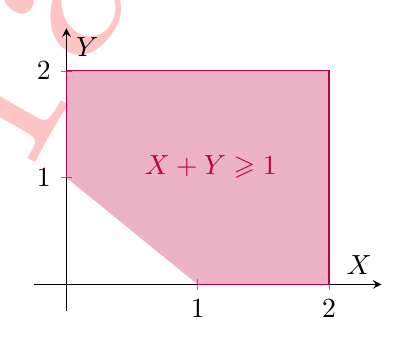
\begin{tikzpicture}
            \begin{axis}[
                width = 6 cm,
                xmin = -0.25, xmax = 2.4,
                ymin = -0.25, ymax = 2.4,
                xlabel = $X$,
                xtick distance = 1,
                ylabel = $Y$,
                ytick distance = 1,
            ]                
                \addplot [
                    draw=purple,
                    fill=purple,
                    fill opacity=0.3,
                ] coordinates {(0, 1) (0, 2) (2, 2) (2, 0) (1, 0)};                
                \node at (axis cs: 1.1, 1.1) {\textcolor{purple}{$X + Y \geq 1$}};
            \end{axis}
        \end{tikzpicture}
        \end{center}

        Widzimy, że szukane zdarzenie zajmuje dokładnie $\frac{7}{8}$ całego kwadratu $2 \times 2$. Odpowiedź jest więc prawdziwa.

        \item $Z$ nie ma rozkładu jednostajnego, intuicyjnie widać, że np. częściej wypadnie wynik 2 niż 0. Żeby się o tym przekonać, możemy obliczyć funkcję gęstości $Z$. Użyjemy znanego nam wzoru na gęstość zmiennej będącej sumą dwóch niezależnych zmiennych losowych:
        $$f_Z(x) = \int_{-\infty}^{+\infty} f_X(y) f_Y(x - y) \dy$$

        Gęstości $f_X, f_Y$ są takie same i, z definicji rozkładu jednostajnego, są dane wzorem
        $$
        f_X(x) = \begin{cases} 
            \frac{1}{2} & \text{dla } x \in [0, 2], \\
            0 & \text{wpp.}
        \end{cases}
        $$

        Ponieważ $f_X, f_Y$ są niezerowe wyłącznie w przedziale $[0, 2]$, ograniczymy całkowanie do tego przedziału. Obliczamy:
        \begin{itemize}
            \item dla $f_X(y) \neq 0$, czyli $x \in [0, 2]$:
            $$f_Z(x) = \int_{0}^{x} f_X(y) f_Y(x - y) \dy = \int_{0}^{x} \frac{1}{2} \cdot \frac{1}{2} \dy = \frac{1}{4} \int_{0}^{x} \dy = \frac{1}{4} \cdot y \big|_0^x = \frac{x}{4}$$

            \item dla $f_Y(x - y) \neq 0$, czyli $x \in [2, 4]$:
            $$f_Z(x) = \int_{x - 2}^{2} f_X(y) f_Y(x - y) \dy = \int_{x - 2}^{2} \frac{1}{2} \cdot \frac{1}{2} \dy = \frac{1}{4} \int_{x - 2}^{2} \dy = \frac{1}{4} \cdot y \big|_{x - 2}^2 = \frac{1}{4}\big(2 - (x - 2)\big) = 1 - \frac{x}{4}$$
        \end{itemize}

        Ostatecznie funkcją gęstości $Z$ jest więc
        $$
        f_Z(x) = \begin{cases}
            \frac{x}{4} & \text{dla } x \in [0, 2), \\
            1 - \frac{x}{4} & \text{dla } x \in [2, 4], \\
            0 & \text{wpp.}
        \end{cases}
        $$
        i pokazuje to, że $Z$ nie ma rozkładu jednostajnego.

        \item Z nierówności Czebyszewa mamy, że $P(|\E Z - Z| \geq 1) \leq \Var Z$. Nietrudno pokazać, że wariancja $Z$ jest równa $\frac{2}{3}$: ze wzoru na wariancję rozkładu jednostajnego $\rpUnif(0, 2)$ mamy
        $$\Var X = \Var Y = \frac{(2 - 0)^2}{12} = \frac{1}{3},$$
        a skoro $Z$ jest sumą dwóch niezależnych zmiennych, możemy skorzystać z addytywności wariancji:
        $$\Var Z = \Var X + \Var Y = \frac{2}{3}$$
    \end{enumerate}

    % Grześ + Jasiek
    \sol Niech $F_{X}(t)$ będzie dystrybuantą pewnej zmiennej losowej $X$. Załóżmy, że $F_{X}(1)=\frac{1}{3}$. Wynika z tego, że
    \answerss{istnieje takie $t$, że $F_{X}(t) = 1$}{$F_X(2) > \frac{1}{3}$}{istnieje takie $t$, że $F_{X}(t) < \frac{1}{4}$}{NIE}{NIE}{TAK}

    \begin{enumerate}[\bf A.]
        \item Zgodnie z własnościami dystrybuanty, mamy pewność, że $\Lim_{x \to \infty} F_X(x) = 1$, ale to niekoniecznie oznacza, że dla pewnego argumentu wartość 1 jest osiągana. Istotnie, nietrudno o przykład, w którym prosta $y = 1$ jest asymptotą poziomą; dzieje się tak choćby dla standardowego rozkładu normalnego:

        \begin{center}
            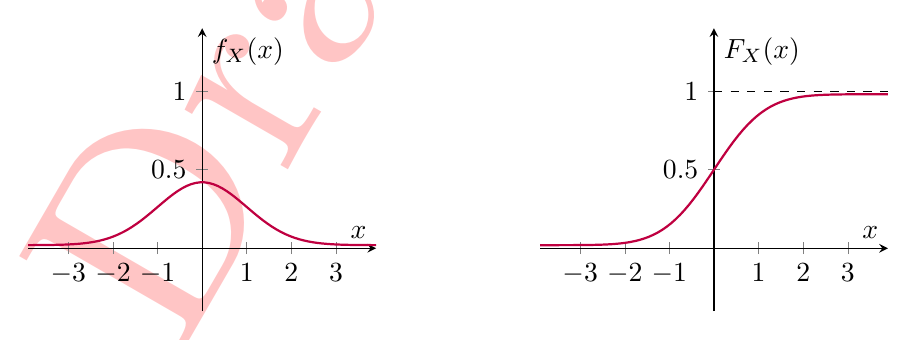
\begin{tikzpicture}
                \begin{axis}[
                    width = 6cm,
                    xmin = -3.9, xmax = 3.9,
                    ymin = -0.4, ymax = 1.4,
                    xtick distance = 1,
                    ylabel = $f_X(x)$,
                    ytick distance = 0.5,
                    samples = 100
                ]
                    \addplot[thick, purple] {0.02 + (0.4 * e^(-0.5 * x^2))};
                \end{axis}
                
                \begin{axis}[
                    width = 6cm,
                    xmin = -3.9, xmax = 3.9,
                    ymin = -0.4, ymax = 1.4,
                    xtick distance = 1,
                    ylabel = $F_X(x)$,
                    ytick distance = 0.5,
                    samples = 100,
                    at = {(6.5cm, 0)}
                ]
                    \addplot[thick, purple] {0.02 + (0.48 * (1 + tanh(sqrt(pi)/2 * (x + 0.044715 * x^3))))};
                    \draw[dashed] (axis cs: 0, 1) -- (axis cs: 5, 1);
                \end{axis}
            \end{tikzpicture}
        \end{center}

        Wówczas nie istnieje żadne $t \in \RR$, dla którego $F_X(t) = 1$.

        \item Dystrybuanta jest funkcją niemalejącą, co oznacza, że $F_X(2) \geq \frac{1}{3}$. Może więc być $F_X(2) = \frac{1}{3}$, co pokazuje fałszywość odpowiedzi.

        \item Ponieważ $\Lim_{x \to -\infty} F_X(x) = 0$, dla bardzo małych argumentów będziemy uzyskiwali bardzo małe wartości, na pewno mniejsze od $\frac{1}{4}$.
    \end{enumerate}

    \sol Niech $X$ i $Y$ będą niezależnymi zmiennymi losowymi. Wynika z tego, że
    \answerss{jeśli $X$ i $Y$ mają rozkład Poissona, to $X - Y$ też}{jeśli $X$ i $Y$ mają rozkład normalny, to $X - Y$ też}{jeśli $X$ i $Y$ mają rozkład geometryczny, to $X - Y$ też}{NIE}{TAK}{NIE}

    \begin{enumerate}[\bf A.]
        \item Niech $X \sim \rpPois(\lambda_X)$ oraz $Y \sim \rpPois(\lambda_Y)$. Takie zmienne modelują liczbę wystąpień pewnego nieprzewidywalnego zdarzenia w ustalonym przedziale czasu, przy czym zdarzenia te mają średnią częstość wystąpienia odpowiednio $\lambda_X, \lambda_Y$.

        O ile zmienna $X + Y$ ma rozkład Poissona (badamy łączne wystąpienia obu niezależnych zdarzeń) z parametrem $\lambda_X + \lambda_Y$, o tyle $X - Y$ napotyka na problem: zmienne o rozkładzie Poissona przyjmują wartości całkowite nieujemne, podczas gdy różnica $\lambda_X - \lambda_Y$ może potencjalnie przyjąć wartości mniejsze od 0.

        \item Zgodnie ze znanym nam faktem, różnica dwóch niezależnych zmiennych losowych o rozkładach normalnych odpowiednio $\rpN(\mu_X, \sigma_X)$ oraz $\rpN(\mu_Y, \sigma_Y)$ ma również rozkład normalny z wartością oczekiwaną $\mu_X - \mu_Y$ i odchyleniem standardowym $\sqrt{\sigma_X^2 + \sigma_Y^2}$.

        \item Kontrargument jest bardzo podobny jak w podpunkcie \textbf{A.} Zmienna o rozkładzie geometrycznym może przyjmować wyłącznie wartości całkowite dodatnie, a różnica $X - Y$ potencjalnie przyjmie wartość ujemną bądź zerową.
    \end{enumerate}

    \sol Niech $X$ i $Y$ będą dwiema niezależnymi zmiennymi losowymi o rozkładzie normalnym o wartości oczekiwanej 0 i wariancji 4. Wynika z tego, że
    \answerss
    {$X - Y$ ma taki sam rozkład jak $X + Y$}
    {odchylenie standardowe zmiennej losowej $X - Y$ jest równe 4}
    {dla $a, b > 0$ zmienna losowa $aX + bY$ ma rozkład normalny}
    {TAK}{NIE}{TAK}

    \begin{enumerate}[\bf A.]
        \item Korzystając ze znanych nam faktów na temat rozkładu sumy i różnicy dwóch niezależnych zmiennych losowych o rozkładzie normalnym otrzymujemy:
        $$X - Y \sim \rpN(\mu_X - \mu_Y, \sqrt{\sigma_X^2 + \sigma_Y^2}) \sim \rpN(0, \sqrt{8})$$
        $$X + Y \sim \rpN(\mu_X + \mu_Y, \sqrt{\sigma_X^2 + \sigma_Y^2}) \sim \rpN(0, \sqrt{8})$$

        \item Jak pokazaliśmy w podpunkcie \textbf{A.}, odchylenie standardowe zmiennej $X - Y$ jest równe $\sqrt{8}$.

        \item Nietrudno intuicyjnie zauważyć, że zmienne $aX, bY$ mają rozkład normalny o przeskalowanych wartościach względem $X$ i $Y$. Ponieważ suma niezależnych zmiennych o rozkładzie normalnym ma również rozkład normalny, odpowiedź jest prawdziwa.
    \end{enumerate}
\end{solutions}



\chapter{Algorytmy i struktury danych}

Materiały teoretyczne zostały opracowane na podstawie slajdów Krzysztofa Diksa. \; \textbf{\red{(przyp. red.: potrzebny link do źródła)}}

\section*{Podstawa programowa}
\begin{enumerate}
    \item Kryteria oceny \textbf{efektywności algorytmów}.
    \item \textbf{Koszt zamortyzowany}.
    \item Podstawowe \textbf{algorytmy sortowania}.
    \item \textbf{Słowniki} i metody ich realizacji.
    \item \textbf{Kolejki priorytetowe} i metody ich realizacji.
\end{enumerate}

\section{Poprawność i efektywność algorytmów}
Powiemy, że algorytm $A$ jest (całkowicie) \textbf{poprawny} względem specyfikacji $\langle \alpha, \beta \rangle$, jeśli spełnia następujące warunki:
\begin{itemize}
    \item \textbf{częściowa poprawność}
    
    Dla każdych danych wejściowych spełniających warunek początkowy $\alpha$, jeśli obliczenie algorytmu $A$ kończy się prawidłowo, wyniki spełniają warunek $\beta$.
    
    \item \textbf{określoność obliczeń}
    
    Dla każdych danych wejściowych spełniających warunek początkowy $\alpha$ obliczenie algorytmu $A$ nie jest przerwane.
    
    \item \textbf{własność stopu}
    
    Dla każdych danych wejściowych spełniających warunek początkowy $\alpha$ obliczenie algorytmu $A$ nie jest nieskończone.
\end{itemize}

\subsection{Złożoność obliczeniowa algorytmu}
Interesują nas dwa typy złożoności:
\begin{itemize}
    \item \textbf{pamięciowa}
    \begin{enumerate}
        \item[a.] ilość pamięci niezbędna do wykonania algorytmu;
        \item[b.] jednostka miary: słowo pamięci maszyny.
    \end{enumerate}
    \item \textbf{czasowa}
    \begin{enumerate}
        \item[a.] czas pracy niezbędny do zrealizowania algorytmu;
        \item[b.] jednostka miary: \textbf{operacja dominująca}, czyli liczba wszystkich operacji jednostkowych wykonywanych przez algorytm powinna być ,,proporcjonalna'' do liczby wszystkich operacji dominujących. Intuicyjnie myślimy o niej jak o operacji, która najbardziej wpływa na czas działania algorytmu. 
    \end{enumerate}
\end{itemize}

Wprowadźmy oznaczenia:
\begin{itemize}
    \item $D_n$ – zbiór możliwych danych wejściowych rozmiaru $n$
    \item $t(d)$ – liczba operacji dominujących dla zestawu danych $d$
    \item $X_n$ – zmienna losowa, której wartością jest $t(d)$ dla $d \in D_n$
    \item $E[X_n]$ - wartość oczekiwana $X_n$
    \item $p_{n,k}$ - prawdopodobieństwo, że dla danych rozmiaru $n$ algorytm wykona $k$ operacji dominujących
\end{itemize}

Przez \textbf{pesymistyczną} złożoność czasową algorytmu rozumie się funkcję
\begin{align*}
    W(n) = \sup \{t(d): d \in D_n\}
\end{align*}

Przez \textbf{oczekiwaną} złożoność czasową algorytmu rozumie się funkcję
\begin{align*}
    A(n) = \sum_{k \geq 0} k \cdot p_{n, k} = E[X_n]
\end{align*}

Intuicyjnie, pesymistyczna złożoność czasowa opisuje zachowanie algorytmu w najgorszym możliwym przypadku, natomiast oczekiwana złożoność czasowa zachowanie w przeciętnym przypadku.
\bigskip

\textbf{Algorytm w miejscu} poza pamięcią na przechowywanie danych, potrzebuje tylko dodatkowej pamięci stałego rozmiaru niezależnie od rozmiaru danych. 

\textbf{Algorytm stabilny} zachowuje względny porządek elementów o tych samych wartościach (np. przy sortowaniu nie zamienia miejscami takich samych elementów).

\begin{example}
    Obliczymy złożoność czasową sortowania przez wstawianie (ang. \textit{insertion sort}). Na wejściu dana jest tablica $a[1...n]$, którą chcemy posortować.
    \begin{cpp}
        a[0] = -INF;              // strażnik, dostatecznie mała wartość
        for (int i = 2; i <= n; i++) {
            v = a[i];
            j = i - 1;
            while (v < a[j]) {    // operacja dominująca
                a[j + 1] = a[j];
                j = j - 1;
            }
            a[j + 1] = v;
        }
    \end{cpp}
    Inwersja w ciągu $a$ to para indeksów $(i, j)$, $1 \leq i < j \leq n$, taka że $a[i] > a[j]$, czyli że element większy znajduje się przed mniejszym. Liczbę inwersji w tablicy $a$ oznaczamy przez $\text{Inv}(a)$. W oczywisty sposób zachodzi $0 \leq \text{Inv}(a) \leq \frac{1}{2}n(n - 1)$.
    
    Złożoność czasowa algorytmu sortowania przez wstawianie mierzona liczbą wykonania operacji dominującej \texttt{v < a[j]}, wynosi $n - 1 + \text{Inv}(a)$, ponieważ dla każdej inwersji $(i, j)$ wykonamy zamianę miejscami elementów $a[i], a[j]$. Dodatkowo, przed wyjściem z pętli \texttt{while} wykonamy jedno porównanie, które nie będzie spełniało warunku pętli.

    Z tego wynika, że pesymistyczna złożoność czasowa algorytmu sortowania przez wstawianie wynosi
    \begin{align*}
        W(n) = n - 1 + \frac{1}{2} \cdot n \cdot (n-1)
    \end{align*}
    Insertion sort jest algorytmem w miejscu oraz stabilnym.
\end{example}

\subsection{Notacja asymptotyczna}
Rozważamy funkcje o argumentach będących nieujemnymi liczbami całkowitymi i o nieujemnych, rzeczywistych wartościach.
\begin{itemize}
    \item Dla danej funkcji $g(n)$ przez $\purple{O(g(n))}$ oznaczamy zbiór funkcji
    \begin{align*}
        O(g(n)) = \{f(n): \text{ istnieją dodatnie stałe } c, n_0 \text{, takie że } \forall_{n \geq n_0} \; 0 \leq f(n) \leq c \cdot g(n) \}
    \end{align*}
    Piszemy $f(n) = O(g(n))$, gdy $f(n) \in O(g(n))$. Możemy o tym myśleć jak o \textbf{ograniczeniu z~góry} tempa wzrostu $f$ przez $g$, podobnie jak to robimy na analizie matematycznej.

    \item Dla danej funkcji $g(n)$ przez $\purple{\Omega(g(n))}$ oznaczamy zbiór funkcji
    \begin{align*}
        \Omega(g(n)) = \{f(n): \text{ istnieją dodatnie stałe } c, n_0 \text{, takie że } \forall_{n \geq n_0} \; 0 \leq c \cdot g(n) \leq f(n) \}
    \end{align*}
    Piszemy $f(n) = \Omega(g(n))$, gdy $f(n) \in \Omega(g(n))$. Możemy o tym myśleć jak o notacji przeciwnej do $O$, a więc jak o \textbf{ograniczeniu z~dołu} tempa wzrostu $f$ przez $g$.

    \item Dla danej funkcji $g(n)$ przez $\purple{\Theta(g(n))}$ oznaczamy zbiór funkcji
    \begin{align*}
        \Theta(g(n)) = \{f(n): \text{ istnieją dodatnie stałe } c_1, c_2, n_0 \text{, takie że } \forall_{n \geq n_0} \; 0 \leq c_1 \cdot g(n) \leq f(n) \leq c_2 \cdot g(n) \}
    \end{align*}
    Piszemy $f(n) = \Theta(g(n))$, gdy $f(n) \in \Theta(g(n))$. Oznacza to, że tempo wzrostu $f$~i~$g$~jest takie samo, a więc zachodzi jednocześnie $f(n) = \Omega(g(n))$ oraz $f(n) = O(g(n))$.
\end{itemize}

\begin{example}
    Kontynuujemy przykład z algorytmem insertion sort. Przypomnijmy obliczoną wcześniej złożoność pesymistyczną:
    \begin{align*}
        W(n) = n - 1 + \frac{1}{2} \cdot n \cdot (n-1) = \frac{n^2}{2} + \frac{n}{2} - 1 
    \end{align*}
    Dzięki notacji asymptotycznej możemy więc powiedzieć, że pesymistyczna złożoność algorytmu insertion sort to $\Theta(n^2)$.

    Obliczmy złożoność oczekiwaną $A(n)$. Dla każdej pary różnych indeksów $i, j$ utworzą one inwersję z prawdopodobieństwem równym $\frac{1}{2}$. Z niezależności wartości oczekiwanej uzyskujemy
    \begin{align*}
        A(n) = n - 1 + \frac{1}{2} \cdot \frac{1}{2} \cdot n \cdot (n-1) = \frac{n^2}{4} + \frac{3n}{4} - 1
    \end{align*}
    Zatem oczekiwana złożoność algorytmu insertion sort to również $\Theta(n^2)$.
\end{example}

% TODO
\begin{editorsnote}
    W części teoretycznej brak informacji o koszcie zamortyzowanym, jednak zawarta tu teoria jest wystarczająca do rozwiązania zadań z przeanalizowanych na potrzeby tego repetytorium archiwalnych egzaminów.
\end{editorsnote}

\begin{problems}
    \prob Agata i Bartek grają w grę polegającą na tym, że Agata wybiera dwie liczby ze zbioru $\{1, 2, ..., n\}$, a Bartek zadaje pytania o wybrany podzbiór i dowiaduje się, czy co najmniej jedna z wybranych liczb znajduje się w nim. Liczba zapytań wystarczających do określenia przez Bartka obu liczb jest
    \answers{$O(n)$}{$O(\sqrt{n})$}{$O(\log{n})$}
\end{problems}

\section{Kolejki priorytetowe}

\textbf{Kopiec} to struktura danych oparta na drzewie. We wszystkich wierzchołkach trzymamy wartości, zwane \textbf{kluczami}.
Wartość w rodzicu wierzchołka jest zawsze mniejsza (lub zawsze większa) od wartości potomka.

% TODO
\begin{editorsnote}
    Brakuje tu opisu kopca binarnego, a pojawia się on w dalszej części teorii.
\end{editorsnote}

\subsection{Kopiec zupełny}

\textbf{Kopiec zupełny} to kopiec binarny, w którym liście występują tylko na ostatnim i przedostatnim poziomie, spójnie ułożone od lewej do prawej. Jego wysokość zatem jest rzędu $O(\log n)$, gdzie $n$ to liczba wierzchołków.

Operacja dodania elementu do takiego kopca polega w uproszczeniu na:
\begin{itemize}
    \item Jeśli dodawany element jest większy (zakładamy typ MAX) od korzenia, to zamieniamy je. W wyniku tej operacji wciąż mamy jeden element do dołożenia do poddrzewa. 
    \item Wyliczamy, czy nadmiarowy element powinien trafić do lewego czy prawego poddrzewa, żeby utrzymać ,,zupełność'' kopca.
    \item Rekurencyjnie dodajemy element do wybranego poddrzewa.
\end{itemize}

Wierzchołki kopca ponumerujemy od $1$ do~$n$, tak że ojcem wierzchołka $i$ jest wierzchołek o numerze $\lfloor \frac{i}{2} \rfloor$, a~$2i$ oraz $2i + 1$ to odpowiednio jego lewy i prawy syn (o ile istnieją). Wartości w wierzchołkach będziemy trzymać w tablicy $a$.

Jeśli wierzchołki o numerach $[l + 1, \dots, r]$ spełniają własność kopca,
to następująca procedura sprawi, że będzie ją spełniać też wierzchołek $l$.
\begin{cpp}
    void DownHeap(l, r) {
        int i = l, j = 2 * i, v = a[i];
        while (j <= r) { // dopóki istnieje syn wierzchołka
            // sprawdzamy, czy prawy syn ma większą wartość
            if (j + 1 <= r && a[j] < a[j + 1])
               j = j + 1; 
    
            // czy nie spełnia wartości kopca?
            if (v < a[j]) {
                // podnosimy wartość z syna 
                a[i] = a[j]; 
                // schodzimy niżej
                i = j;
                j = 2 * i;
            } else {
                // wszystko jest okej
                break;
            }
        }
        a[i] = v;
    }
\end{cpp}

\subsection{Kopiec dwumianowy (kolejka dwumianowa)}

\textbf{Drzewo dwumianowe} $B_k$ jest zdefiniowane rekurencyjnie. Jest to drzewo $B_{k - 1}$ z drugim drzewem $B_{k - 1}$ przyłączonym krawędzią do korzenia.
Drzewo $B_0$ składa się z pojedynczego wierzchołka. Widać zatem, że $|B_k| = 2^k$.

\begin{figure}[H]
    \centering
    \includegraphics[scale=0.5]{rozdziały/images/ASD/drzewa_dwumianowe.png}
    \caption{Drzewa dwumianowe}
\end{figure}

\textbf{Kolejka dwumianowa} składa się z lasu drzew dwumianowych o parami różnych rozmiarach, których rozmiary w sumie dają $n$. W każdym drzewie elementy są rozmieszczone tak, żeby wartości spełniały porządek kopcowy.

Dostęp do najmniejszego elementu obywa się przez wskaźnik na korzeń z najmniejszą wartością.

W takiej kolejce ważne są dwie operacje:
\begin{itemize}
    \item Join($T_1$, $T_2$) łączy dwa drzewa tego samego stopnia w jedno drzewo o stopniu o 1 większym z zachowaniem porządku kopcowego. Złożoność: $O(1)$.
    \item Union($Q_1$, $Q_2$) łączy dwie kolejki dwumianowe $Q_1, Q_2$ w jedną kolejkę $Q_1$, korzystając z operacji Join. Złożoność: $O(\log n)$.
\end{itemize}

Powyższe operacje wykorzystuje się, żeby zaimplementować kolejkę priorytetową. Na przykład, wstawienie elementu do kolejki to Union() z jednoelementową kolejką.

\subsection{Kopiec Fibonacciego}

\textbf{Kopiec Fibonacciego} składa się z listy dwukierunkowej korzeni kolejnych drzew, tym razem już może być wiele drzew o tych samych rozmiarach. Utrzymywany jest wskaźnik na korzeń z najmniejszą wartością.

Operacja znajdowania minimum jest zatem trywialna, i działa w czasie stałym.

Wstawianie elementu polega na stworzeniu nowego jednoelementowego drzewa i dodaniu go do listy.

Operacja usunięcia najmniejszego elementu przebiega w 3 fazach.
\begin{enumerate}
    \item Usuwamy korzeń zawierający minimalny element, a jego dzieci (z poddrzewami) dołączamy do listy drzew kopca.
    \item Musimy uaktualnić wskaźnik na minimalny klucz. Na liście korzeni może być $n$ elementów, zatem najpierw będziemy łączyć drzewa o tym samym stopniu (liczba synów korzenia).
    \item Uaktualniamy wskaźnik na minimum.
\end{enumerate}
Amortyzowany koszt tej operacji to $O(\log n)$. Jeśli wcześniej wykonywaliśmy same operacje dodawania wierzchołków i usuwania minimum, to otrzymamy w wyniku tej operacji kopiec dwumianowy.

Operacja zmniejszenia wartości (używana w opisanym później algorytmie Dijkstry) zaczyna od zmniejszenia wartości zadanego wierzchołka
i w razie, gdy nowa wartość zaburza porządek kopcowy (wierzchołek ma wartość mniejszą niż rodzic), wywołujemy operację odcinania rozważanego wierzchołka.

Operacja odcinania wierzchołka $x$ odcina go od ojca $y$ i dołącza do listy korzeni kopca. Dodatkowo, $y$ zostaje oznaczony jako wierzchołek, który utracił jedno dziecko. 
Przy próbie odcięcia drugiego dziecka, nie odcinamy go, tylko wywołujemy $cut(y)$, przenosząc operację w górę drzewa tak długo, aż dojdziemy do korzenia, lub wierzchołka który nie utracił jeszcze syna.

Dzięki tym operacjom otrzymujemy koszt amortyzowany $O(1)$ operacji zmniejszenia wartości klucza.

Nazwa kopca pochodzi od tego, że minimalny rozmiar drzewa o stopniu $d$ to liczba Fibonacciego o indeksie $(d + 2)$

\begin{figure}[H]
    \centering
    \includegraphics[scale=0.5]{rozdziały/images/ASD/kopiec_fibonacciego.png}
    \caption{Drzewa o najmniejszym możliwym rozmiarze w kopcu Fibonacciego}
\end{figure}

\subsection{Porównanie}

Zestawienie złożoności najważniejszych operacji (złożoności oznaczone gwiazdką są amortyzowane):

\begin{tabular}{ |l|c|c|c| }
    \hline
    operacja & kopiec zupełny & kopiec dwumianowy  & kopiec Fibonacciego \\
    \hline
    inicjalizacja pustego kopca & $O(1)$ & $O(1)$ & $O(1)$ \\
    \hline
    podanie najmniejszego elementu & $O(1)$ & $O(1)$ & $O(1)$ \\
    \hline
    usunięcie najmniejszego elementu & $O(\log n)$ & $O(\log n)$ & $O(\log n)$* \\
    \hline
    wstawienie elementu & $O(\log n)$ & $O(\log n)$ & $O(1)$* \\
    \hline
    zmniejszenie jednej wartości & $O(\log n)$ & $O(\log n)$ & $O(1)$* \\
    \hline
\end{tabular}

\begin{problems}
    \prob Do początkowo pustego kopca Fibonacciego typu min wstawiamy kolejno rekordy o priorytetach odpowiednio $1, 2, ..., 2020$, otrzymując kopiec $T$, a następnie wykonujemy operację \texttt{DeleteMin}, otrzymując kopiec $T'$. Wynika z tego, że
    \answers{kopiec $T$ składa się z co najwyżej 8 drzew}{kopiec $T'$ składa się z co najwyżej 8 drzew}{najwyższe drzewo w kopcu $T'$ ma wysokość (tzn. największą możliwą liczbę krawędzi od korzenia do liścia w drzewie) co najmniej $10$}
\end{problems}


\section{Algorytmy sortowania}
\subsection{Insertion sort}
Inaczej sortowanie przez wstawianie, opisane powyżej. Cechy:
\begin{itemize}
    \item w miejscu
    \item stabilny
    \item złożoność zależna od liczby inwersji
    \item oczekiwana oraz pesymistyczna złożoność kwadratowa
\end{itemize}

\subsection{Bubble sort}
Inaczej sortowanie bąbelkowe.
\begin{cpp}
    for (int i = n; i >= 2; i--) {
        for (int j = 1; j <= i - 1; j++) {
            if (a[j] > a[j + 1])       // #porównania - wszystkie możliwe czyli n * (n - 1) / 2
                swap(a[j], a[j + 1]);  // #zamiany = Inv(a)
        }
    }
\end{cpp}
Cechy:
\begin{itemize}
    \item w miejscu (+);
    \item stabilny (+);
    \item liczba zamian zależna od liczby inwersji (+/-);
    \item kwadratowa liczba porównań, niezależnie do danych (-).
\end{itemize}

\subsection{Selection sort}
Inaczej sortowanie przez wybieranie.
\begin{cpp}
    for (int i = n; i >= 2; i--) {
        i_max = 1;
        for (int j = 2; j <= i; j++) {
            if (a[j] > a[i_max])   // #porównania = n * (n - 1) / 2
                i_max := j;
        }
        swap(a[i], a[i_max]);  // #zamiany = n - 1
    }
\end{cpp}
Cechy:
\begin{itemize}
    \item w miejscu (+);
    \item nie jest stabilny (-);
    \item mała liczba zamian (+);
    \item kwadratowa liczba porównań, niezależnie do danych (-).
\end{itemize}

\subsection{Heap sort}
Inaczej sortowanie przez kopcowanie. Dzięki użyciu kopca otrzymujemy szybszy selection sort, ponieważ umiemy znajdować maksimum w logarytmicznym czasie.
\begin{cpp}
    // Budowa kopca.
    // Zauważmy, że n / 2 wartości w liściach może zostać przepisanych z tablicy a.
    for (int i = n / 2; i >= 1; i--)
        DownHeap(i, n);

    // Niezmiennik: a[1..i] <= a[i+1] <= ... <= a[n] oraz heap(1,i).
    for (int i = n; i >= 2; i--) {
        swap(a[1], a[i]);
        DownHeap(1, i - 1);
    }
\end{cpp}
Cechy:
\begin{itemize}
    \item w miejscu (+);
    \item nie jest stabilny (-);
    \item pesymistyczny czas działania $\Theta(n \log n)$ (+).
\end{itemize}

\subsection{Merge sort}
Inaczej sortowanie przez scalanie.
\begin{cpp}
    // b[1..n] – globalna tablica pomocnicza
    // Niezmiennik: przy wywołaniu funkcji posortowane jest a[l...s] oraz a[s+1...r].
    // Po wywołaniu posortowane będzie a[l...r].
    void merge(int l, int r, int s) {
        i = l;
        j = s + 1;
        k = l - 1;
        while (i <= s && j <= r) {
            k = k + 1;
            if (a[i] <= a[j]) {     // #porównania <= r - l
                b[k] = a[i];
                i = i + 1;
            }
            else {
                b[k] = a[j];
                j = j + 1;
            }
        }
        if (i > s)
            b[k+1...r] = a[j...r]
        else
            b[k+1...r] = a[i...s]
        a[l...r] = b[l...r]
    }

    void merge_sort(int l, int r) {
        if (l < r) {
            s = (l + r) / 2;
            merge_sort(l, s);
            merge_sort(s + 1, r);
            merge(l, r, s);
        }
    }

    merge_sort(1, n);
\end{cpp}

Cechy:
\begin{itemize}
    \item nie jest w miejscu (-) aczkolwiek istnieje trudniejsza wersja w miejscu;
    \item stabilny (+);
    \item pesymistyczny czas działania $\Theta(n \log n)$ (+);
    \item bardzo mało porównań (+);
    \item sporo przypisań, możliwa redukcja (-/+).
\end{itemize}

\subsection{Quick sort}
Intuicyjnie jest to algorytm, które po prostu buduje drzewo BST.
\begin{cpp}
    // Niech S będzie zbiorem, który chcemy posortować.
    // elem S zwraca wszystkie elementy zbioru S.
    void quick_sort(S) {
        if (|S| <= 1) {
            print(elem S);                       // jedyny element zbioru S
        }
        else {
            x = pivot(S);                        // element dzielący
            S_less = {y: elem S && y < x};       // zbiór elementów mniejszych niż x
            S_greater = {y: elem S && y > x};    // zbiór elementów większych niż x
            quick_sort(S_less);
            print(x);
            quick_sort(S_greater);
        }
    }
\end{cpp}

\begin{figure}[H]
    \centering
    \includegraphics[scale=0.3]{rozdziały/images/ASD/quick_sort.png}
    \caption{Ilustracja działania algorytmu quick sort.}
\end{figure}

W powyższym przykładzie jako pivot wybieramy zawsze pierwszy element sortowanego zbioru. Takie drzewo obliczeń może być niskie (wysokości $O(\log n)$) lub wysokie (np. dla $S = \{1, 2, ..., n\})$. Przy losowym wyborze pivota algorytm ten działa jednak w oczekiwanej złożoności $\Theta(n \log n)$.

Cechy:
\begin{itemize}
    \item prawie w miejscu (-/+);
    \item nie jest stabilny (-);
    \item pesymistyczna złożoność $\Theta(n^2)$ (-);
    \item oczekiwana złożoność $\Theta(n \log n)$ (+);
    \item bardzo dobrze sprawdza się w praktyce.
\end{itemize}

\subsection{Count sort}
Inaczej sortowanie przez zliczanie. Działa dobrze przy założeniu, że elementy tablicy $a$ nie są zbyt duże.
\begin{cpp}
    // b - tablica zliczająca liczbę wystąpień elementów a
    m = max(a) + 1;
    b = [0] * m;
    for (int i = 1; i <= n; i++)
        b[a[i]]++;

    // Dla każdej wartości tablicy a wyznaczamy ostatnią pozycję,
    // na której wystąpi ona w posortowanej tablicy.
    for (int i = 1; i <= m - 1; i++)
        b[i] += b[i - 1];

    // t - tablica pomocnicza
    for (int i = n; i >= 1; i--) {
        t[b[a[i]]] = a[i];
        b[a[i]]--;
    }

    a = t;
\end{cpp}
Cechy:
\begin{itemize}
    \item nie jest w miejscu (-);
    \item stabilny (+);
    \item złożoność $\Theta(n + m)$ (-/+);
    \item dla $m = O(n)$ algorytm liniowy (+).
\end{itemize}

\subsection{Bucket sort}
Inaczej sortowanie kubełkowe. Idea taka sama jak w count sorcie, ale utrzymujemy tablicę list zamiast zwykłego countera.
\begin{cpp}
    // Inicjacja pustych kubełków.
    m = max(a) + 1;
    b = {} * m;
    
    // Wypełnienie kubełków.
    for (int i = 1; i <= n; i++)
        b[a[i]].push_back(a[i]);

    // Końcowe scalenie
    wynik = {};
    for (int i = 0; i <= m - 1; i++)
        wynik.append(b[i]);
\end{cpp}
Cechy:
\begin{itemize}
    \item nie jest w miejscu (-);
    \item stabilny (+);
    \item złożoność $\Theta(n + m)$ (-/+);
    \item dla $m = O(n)$ algorytm liniowy (+).
\end{itemize}

\subsection{Sortowanie leksykograficzne słów tej samej długości}
Dane:
\begin{itemize}
    \item dodatnie liczby całkowite $n, k, m$;
    \item $s[1..n]$ - tablica słów o długości $k$ nad alfabetem $\{0, 1, ..., m - 1\}$;
    \item oznaczenie: $s[i][j]$ – $j$-ta litera w słowie $s[i]$. 
\end{itemize}
Wynik:
\begin{itemize}
    \item $w[1...n]$ – permutacja indeksów $1, ..., n$ wyznaczająca porządek leksykograficzny słów $s$.
\end{itemize}
\begin{cpp}
    w[1...n] = [1, 2, ..., n];
    for (int j = k; j >= 1; j--) {
        posortuj w stabilnie w względem znaków z pozycji j w słowach;
    }
\end{cpp}
Do posortowania stabilnie możemy wykorzystać bucket sort.

Cechy:
\begin{itemize}
    \item stabilny (+);
    \item złożoność $\Theta(k \cdot (n + m))$ (-/+).
\end{itemize}

\subsection{Sortowanie leksykograficzne}
Poprzedni algorytm da się uogólnić na sortowanie leksykograficzne słów różnej długości.

Cechy:
\begin{itemize}
    \item złożoność $\Theta(k \cdot n + m)$ (-/+).
\end{itemize}

\subsection{Inne algorytmy sortowania}
\begin{itemize}
    \item Metoda Shella, usprawnienie insertion sorta, $h$-sortowania.
    \item Sortowanie introspektywne - quick sort z pesymistyczną złożonością $O(n \log n)$.
\end{itemize}

\subsection{Ważny fakt}
Każdy algorytm sortujący \textbf{przez porównania} wykonuje w pesymistycznym przypadku $\Theta(n \log n)$ porównań.


\begin{problems}
    \prob W modelu losowej permutacji, złożoność $\Omega(n^2)$ ma algorytm
    \answers
    {quick sort}
    {insertion sort}
    {heap sort}

    \prob Pesymistyczna złożoność algorytmów sortowania w zależności od liczby inwersji $inv$ to
    \answers{dla insertion sort: $O(\max(n, inv))$}{dla quick sort: $O(n \cdot \log(\max(n, inv)))$}{dla heap sort: $O(n \cdot \log(\max(n, inv)))$}
    
    \prob Ciąg $\delta=\langle\delta_1,\delta_2,\ldots,\delta_n\rangle$ nazywamy $k$-uporządkowanym rosnąco, gdy każdy jego podciąg złożony z~elementów odległych o $k$ jest uporządkowany rosnąco, tzn. $\delta_i<\delta_{i+k}$ dla $i=1,2,\ldots n-k$. Ciąg $\delta$ można uporządkować za pomocą $O(n)$ porównań, gdy jest on
    \answers{jednocześnie 2- i 3-uporządkowany}{2012-uporządkowany}{$\lfloor\log{n}\rfloor$-uporządkowany}
    
    \prob Rozważmy równanie rekurencyjne $$ T(n) = \begin{cases} n & \text{dla }  \; n \leq 1 ,\\ T(\lfloor n/2 \rfloor) + T(\lceil n/2 \rceil ) + n + 1 & \text{dla } \; n > 1 \end{cases} $$
    Wartość $T(n) $
    \answers
    {jest ograniczeniem górnym na liczbę porównań wykonywanych w algorytmie sortowania $n$ różnych elementów przez scalanie}
    {jest ograniczeniem górnym na średnią liczbę porównań w algorytmie sortowania szybkiego dla $n$ różnych elementów, gdy element dzielący jest wybierany losowo z rozkładem jednostajnym}
    {jest rzędu $\Theta (n \log n)$}
\end{problems}

\section{Algorytmy grafowe}

\textbf{Algorytm Dijkstry} w spójnym grafie z krawędziami o nieujemnych wagach szuka najkrótszych ścieżek od wyróżnionego wierzchołka do wszystkich pozostałych.

Pseudokod:
\begin{cpp}
/* s - wierzchołek startowy
 * L - zbiór wierzchołków, dla których znamy już najkrótsze ścieżki
 * R - dopełnienie L
 * w(u, v) - waga krawędzi u -> v
 * N(v) - sąsiedzi wierzchołka v */
begin
    /* inicjacja */
    d(s) := 0, L := {s}, R := V - {s};
    for v in R do d(v) := +inf;
    for v in N(s) do d(v) := w(s, v);

    /* pętla główna */
    while |R| > 0 do
    begin
        v := wierzchołek w R o najmniejszej wadze d
        R := R - {v};
        L := L + {v};
        for u in (R and N(v)) do d(i) := min(d(u), d(v) + w(v, u);
    end
end
\end{cpp}

Złożoność czasowa algorytmu Dijkstry to $O(m \cdot \text{DecreaseKey} + n \cdot \text{DeleteMin})$, gdzie $m$ to liczba krawędzi w grafie, $n$ to liczba wierzchołków, a koszt DecreaseKey oraz DeleteMin zależy od wykorzystanej struktury danych.

\begin{exam}
    Złożoność algorytmu Dijkstry dla spójnego grafu o $n$ wierzchołkach i $m$ krawędziach w implementacji
    \answers{z kopcem zupełnym to $O(m \log n)$}{z kopcem dwumianowym to $O(m + n \sqrt{\log n})$}{z kopcem Fibonacciego to $O(m + n \log n)$}
    
    Złożoność algorytmu Dijkstry to $O(m\cdot\texttt{DecreaseKey}+n\cdot\texttt{DeleteMin})$. W każdym kopcu operacja \texttt{DeleteMin} ma koszt $O(\log{n})$, podobnie jak \texttt{DecreaseKey}, które jedynie w przypadku kopca Fibonacciego amortyzuje się do czasu stałego.

    Zauważmy również, że dla spójnego grafu $m$ jest co najmniej rzędu $n$, a maksymalnie rzędu $n^2$.

    \begin{enumerate}[\bf A.]
        \item Czas będzie $O(m\log{n}+n\log{n})$, ale ponieważ graf jest spójny, to ma co najmniej $\Omega(n)$ krawędzi, więc drugi składnik sumy nic nie wnosi do złożoności i odpowiedzią jest \texttt{TAK}.

        \item Złożoność taka sama, jak dla kopca zupełnego ($O(m \log n)$), więc odpowiedź to \texttt{NIE}.

        \item Wstawiając powyższe złożoności kopca Fibonacciego do wzoru otrzymamy dokładnie taką złożoność, odpowiedź to \texttt{TAK}.
    \end{enumerate}
\end{exam}

\subsection{Algorytmy przeszukiwania grafu}

\textbf{Przeszukiwanie grafu wszerz} (ang. \textit{Breadth First Search} -- BFS) pozwala nam znaleźć 
najkrótsze ścieżki (w~grafie bez wag na krawędziach) w czasie $O(n + m)$, gdzie $n$ to liczba wierzchołków a $m$ to 
liczba krawędzi w~grafie.

\begin{cpp}
/* s - wierzchołek startowy */
deque<int> S = {s}; /* kolejka FIFO */
vector<int> D(n, -1); /* tablica odległości */
D[s] = 0;
while (!S.empty()) {
    int v = S.front();
    S.pop_front();
    for (int u : adj[v]) {
        if (D[u] == -1) {
            D[u] = D[v] + 1;
            S.push_back(u);
        }
    }
}
\end{cpp}

\textbf{Przeszukiwanie grafu w głąb} (ang. \textit{Depth First Search} -- DFS) otrzymujemy, poprzez zastąpienie kolejki FIFO w BFS-ie stosem. 
Można go efektywnie zapisać rekurencyjnie:
\begin{cpp}
vector<bool> vis(n); /* tablica odwiedzonych */
void dfs(int v) {
    vis[v] = true;
    for (int u : adj[v]) {
        if (!vis[u])
            dfs(u);
    }
}
\end{cpp}

Krawędzie, którymi przechodziliśmy przy przeszukiwaniu grafu, tworzą \textbf{drzewo rozpinające} tego grafu. 

Drzewo BFS grafu jest drzewem najkrótszych ścieżek w tym grafie.

Drzewo DFS grafu ma ważną właściwość. Wszystkie krawędzie niedrzewowe łączą przodka z potomkiem lub w drugą stronę. Nigdy nie idą ,,w poprzek'' drzewa -- mogły by być wtedy wykorzystane przez algorytm DFS.

\begin{problems}
    \prob Dany jest graf $G$ o 10 wierzchołkach z wyróżnionym wierzchołkiem $r$. Drzewo rozpinające utworzone przejściem DFS od wierzchołka $r$ ma wysokość $h$ (największa liczba krawędzi od korzenia do liścia). Prawdą jest, że
    \answers
    {jeśli $h = 8$, graf $G$ ma co najwyżej 44 krawędzie}
    {jeśli $h = 2$, graf $G$ ma co najwyżej 15 krawędzi}
    {rozpinające drzewo powstałe algorytmem BFS ma zawsze mniejszą wysokość niż $h$}

    \prob Niech $n$ będzie liczbą całkowitą większą od 1. Wynika z tego, że
    \answers
    {wysokość (czyli największa liczba \emph{krawędzi} od korzenia do liścia) drzewa BFS w grafie dwudzielnym $K_{n,n}$ wynosi 2}
    {wysokość drzewa DFS w grafie dwudzielnym $K_{n,n}$ wynosi $n$}
    {jeżeli $n > 10$, to istnieje spójny graf $n$-wierzchołkowy o $n$ krawędziach, dla którego drzewa BFS i DFS o tym samym korzeniu są takie same}

    \prob $G$ jest 1001-wierzchołkowym grafem dwuspójnym wierzchołkowo. Wynika z tego, że
    \answers
    {jeżeli wysokość pewnego drzewa DFS grafu $G$ wynosi 1000, to $G$ ma cykl Hamiltona}
    {wysokość każdego drzewa BFS grafu $G$ jest nie większa niż 500}
    {wysokość każdego drzewa DFS grafu $G$ jest różna od 2}

    \prob Koszt wykonania algorytmu Dijkstry dla spójnego grafu $n$-wierzchołkowego o $m$ krawędziach wynosi
    \answers{$O(m\log{n})$ w implementacji z kopcem zupełnym}{$O(n\log{n}+m)$ w implementacji z kopcem Fibonacciego}{$O(n^2)$ w implementacji z kolejką dwumianową}

    \prob Wysokość drzewa ukorzenionego mierzymy liczbą krawędzi na najdłuższej ścieżce z korzenia do wierzchołka w tym drzewie. Dany jest spójny $n$-wierzchołkowy graf dwuspójny wierzchołkowo (tzn. bez wierzchołków rozdzielających) o co najmniej 4 wierzchołkach. Prawdą jest, że
    \answers{wysokość każdego drzewa przeszukiwania wszerz w takim grafie jest mniejsza od $n / 2$}{wysokość każdego drzewa przeszukiwania w głąb w takim grafie jest większa od $n / 2$}{wysokość każdego drzewa przeszukiwania w głąb w takim grafie wynosi co najmniej $3$}

    \prob Wysokość drzewa BST zawierającego 100 wierzchołków
    \answers{wynosi co najmniej 49}{wynosi co najmniej 7}{wynosi co najwyżej 99}
\end{problems}

\section{Drzewa BST}

\textbf{Drzewa wyszukiwań binarnych} (drzewa BST -- Binary Search Trees) -- drzewa binarne, w których elementy rozmieszczone są w porządku symetrycznym: dla każdego wierzchołka, wartość w nim (klucz) jest większa od wszystkich wartości w jego lewym poddrzewie oraz mniejsza od wszystkich wartości w jego prawym poddrzewie.

\begin{exam}
    Rozważmy drzewo BST budowane poprzez kolejne wstawianie pewnej permutacji ciągu liczb 1, 2, …, 7. Permutacji takich że powstanie drzewo o wysokości
    \answers{6 jest 64}{5 jest 32}{2 jest 80}
    \bigskip

    \begin{enumerate}[\bf A.]
        \item Aby uzyskać BST o wysokości 6, w każdym kroku budowania drzewa musimy wstawić wierzchołek z najmniejszą lub największą wartością, która nie jest jeszcze wykorzystana (np. w pierwszym kroku wstawimy 1 lub 7). Takich permutacji możemy utworzyć $2^6 = 64$, więc odpowiedź jest prawdziwa.

        \item Rozważmy utworzenie drzewa BST o wysokości 5 w następujący sposób: na początku wstawmy wartość 2, a następnie utwórzmy ścieżkę analogicznie jak w podpunkcie \textbf{A.} z wartości $\{3, 4, 5, 6, 7\}$. Wartość 1 możemy wstawić w dowolne miejsce permutacji, ale później niż wartość 2. To już daje $2^4 \cdot 6 > 32$ opcje, więc odpowiedź to \texttt{NIE}.

        \item Aby otrzymać pełne drzewo binarne, musimy najpierw wstawić wartość 4. Dodatkowo musimy wstawić wartość 2 przed 1 i 3. Analogicznie musimy wstawić wartość 6 przed 5 i 7. Mamy więc $\binom{6}{3} \cdot 2 \cdot 2 = 80$ opcji: wybieramy pozycje dla trójki $\{1, 2, 3\}$, następnie dowolnie permutujemy 1 z 3 oraz 5 z 7. Odpowiedź to \texttt{TAK}.
    \end{enumerate}
\end{exam}

\subsection{Drzewo AVL}
\textbf{Drzewo AVL} to drzewo wyszukiwań binarnych, w którym dla każdego węzła wysokości jego poddrzew różnią się o co najwyżej 1.

Z tego faktu wynika, że wysokość drzewa jest $O(\log n)$.

Implementacja polega na tym, że przy każdej zmianie w drzewie wykonujemy rotacje, żeby drzewo było znowu zbalansowane.

% TODO: dopisać te wzory + przeredagować poniższą ramkę ,,To było na egzaminie'' (po dopisaniu wzorów do części teoretycznej nie trzeba aż tak dużo rozwodzić się nad analizą rozwiązania np. podpunktu B.)
\begin{editorsnote}
    Trzeba tu dopisać wzory na maksymalną i minimalną liczbę wierzchołków drzewa AVL (pojawia się to w praktycznie każdym zadaniu).
\end{editorsnote}

\begin{exam}
    Wysokość drzewa wyszukiwań binarnych mierzymy liczbą krawędzi na najdłuższej ścieżce od korzenia do liścia (węzła z kluczem bez następników). Wysokość drzew z jednym kluczem wynosi $0$. Wysokość drzewa AVL z $2022$ kluczami
    \answers{wynosi co najmniej $11$}{wynosi co najwyżej $22$}{będzie maksymalna, jeśli klucze zostaną wstawione do początkowo pustego drzewa w kolejności rosnącej}
    \bigskip

    \begin{enumerate}[\bf A.]
        \item Dla danej wysokości $h$ maksymalna liczba wierzchołków w AVL drzewie to liczba wierzchołków w pełnym drzewie binarnym, czyli $2^{h+1}-1$. Mając $2022<2047=2^{10+1}-1$ wierzchołki, widzimy, że minimalna wysokość w naszym przypadku będzie równa 10, odpowiedź jest więc fałszywa.

        \item Najmniejsze liczby wierzchołków tworzą ciąg Fibonacciego dany wzorem $F_{n}=F_{n-1}+F_{n-2}+1$: dla $h=0, 1, 2, 3, 4, \ldots$ mamy $\min_n=1,2,4,7,12,\ldots$, bo mając minimalne drzewa dla $n-2$ i $n-1$, chcąc stworzyć minimalne AVL drzewo dla $n$, rysujemy korzeń i podłączamy te dwa drzewa jako prawego i lewego syna, dostając wspomniany wzór. Licząc na palcach (bo ciąg ten rośnie dość szybko), możemy zauważyć, że z 1596 wierzchołkami dostaniemy maksymalnie wysokość 14, a z 2583 -- 15. Wynika stąd, że dla 2022 wierzchołków dostaniemy najwyżej wysokość 14, czyli w szczególności co najwyżej 22 -- odpowiedź to \texttt{TAK}.

        \item Gdy zaczniemy wstawiać klucze w kolejności rosnącej, to szybko zauważymy, że bynajmniej nie maksymalizujemy wysokości drzewa.
    \end{enumerate}
\end{exam}

\subsection{Drzewo splay}
Wykonanie podstawowych operacji na tym drzewie wiąże się z wykonaniem procedury {\ttfamily LocalSplay(x)}, 
która powoduje zmianę struktury drzewa, że węzeł $x$ zostaje umieszczony w korzeniu (przy zachowaniu porządku symetrycznego).

Koszt zamortyzowany tej funkcji jest $O(\log n)$ (pesymistycznie $\Theta(n)$), i taki też koszt mają podstawowe operacje.

\subsection{Drzewo czerwono-czarne}
\textbf{Drzewo czerwono-czarne} - drzewo BST, w którym każdy węzeł jest pokolorowany na czerwono lub czarno, zgodnie z następującymi regułami:
\begin{itemize}
    \item korzeń drzewa jest czarny
    \item każdy czerwony węzeł ma czarnego rodzica
    \item każdy węzeł zewnętrzny (\texttt{NULL}) jest czarny
    \item każda ścieżka (elementarna) z ustalonego węzła do węzła zewnętrznego w jego poddrzewie zawiera tyle samo węzłów czarnych
\end{itemize}

Z tych warunków wynika, że wysokość drzewa jest $O(\log n)$.

\begin{problems}
    \prob O drzewach AVL prawdą jest, że
    \answers{największe drzewo AVL o wysokości 5 ma 64 wierzchołki}{najmniejsze drzewo AVL o wysokości 5 ma 20 wierzchołków}{każde drzewo czerwono-czarne jest AVL drzewem}

    \prob Do początkowo pustego drzewa BST wstawiamy kolejno elementy pewnej permutacji liczb $1,2,\ldots,16$. Liczba permutacji, dla których
    \answers{dostaniemy drzewo o wysokości (czyli maksymalnej liczbie krawędzi na ścieżce od korzenia do liścia) równej 15, wynosi co najwyżej $2^{16}$}{dostaniemy drzewo o wysokości równej 3, wynosi co najmniej $2^{15}$}{w lewym poddrzewie korzenia będzie tylko węzeł z kluczem 1, wynosi co najmniej jeden miliard}

    \prob W zbiorze AVL-drzew o 10 węzłach
    \answers{istnieje drzewo o wysokości (czyli największej liczbie krawędzi od korzenia do liścia) równej 4}{każde drzewo ma wysokość co najmniej 3}{maksymalna różnica liczb węzłów poddrzew korzenia wynosi 5}
\end{problems}

\section{Algorytmy tekstowe}
Po dokładne opisy algorytmów odsyłam do przedmiotowych slajdów, poniżej znajdują się tylko podstawowe fakty, definicje oraz intuicja.

\subsection{Haszowanie}
Służy do reprezentacji elementów pewnego dużego zbioru (klucze) poprzez elementy mniejszego zbioru. Częstym przypadkiem jest zamiana słów na liczby. Oznaczmy duży zbiór przez $U$. Słownik $S$ mapujący klucze na wartości implementujemy w tablicy $a[0..m-1]$, gdzie $m$ jest dużo mniejsze niż rozmiar $U$. Tworzymy funkcję haszującą $h: U \to \{0, ..., m - 1\}$, która odwzorowuje klucze w przestrzeń adresową. $S$ implementujemy w tablicy list $a[0..m-1]$, gdzie $a[i]$ to lista wszystkich kluczy $k$, dla których $h(k) = i$. Tablicę, w której implementujemy słownik nazywamy tablicą z haszowaniem (tablicą haszowaną).

Powiemy, że dwa różne klucze $e$ i $f$ są ze sobą w kolizji, gdy $h(e) = h(f)$.

Cechy dobrej funkcji haszującej:
\begin{itemize}
    \item równomiernie haszuje: losowo wybrany klucz jest z jednakowym prawdopodobieństwem
odwzorowywany na każdą z $m$ pozycji, niezależnie od tego, gdzie zostają odwzorowane inne klucze
    \item łatwo (szybko) obliczalna
\end{itemize}
Najbardziej znanym haszowaniem jest haszowanie modularne: $h(k) = k \mod m$, gdzie $m$ jest liczbą pierwszą daleką od potęgi dwójki.

\subsection{Algorytm KMP}
Służy do rozwiązywania problemu wyszukiwania wzorca w tekście. Niech $\Sigma$ – skończony, niepusty alfabet oraz wzorzec $w[1...m]$, tekst $t[1...n]$ – słowa nad alfabetem $\Sigma$, $1 \leq m \leq n$. Należy znaleźć wszystkie wystąpienia wzorca $w$ w tekście $t$, tzn. należy znaleźć wszystkie takie $i, 1 \leq i \leq n - m + 1$, że $w[1...m] = t[i...i + m - 1]$.
\begin{example}
    Niech $w = [baba]$ oraz $t = [abbababaababab]$. Wzorzec $w$ występuje w tekście $t$ na pozycjach 3, 5 i 10.
\end{example}
Algorytm KMP działa w czasie $O(n + m)$. Zauważmy również, że wzorzec może wystąpić w tekście tylko jeśli jest niedłuższy od tekstu, a więc algorytm działa w czasie $O(n)$.

\subsection{Drzewo trie}
\href{https://pl.wikipedia.org/wiki/Drzewo_trie}{Drzewo trie} to drzewo poszukiwań przechowujące w węzłach fragmenty kluczy. To pozwala przyspieszyć wyszukiwanie, gdy koszt porównania całego klucza jest duży. Znakomicie sprawdzają się więc do utrzymywania np. zbioru słów.

\begin{figure}[H]
    \centering
    \includegraphics[scale=0.75]{rozdziały/images/ASD/trie.png}
    \caption{Przykładowe drzewo trie}
\end{figure}

Działania jakie można zrealizować za pomocą drzew trie:
\begin{itemize}
    \item sprawdzenie, czy słowo długości $k$ jest w drzewie w czasie $O(k)$;
    \item znalezienie najdłuższego prefiksu słowa występującego w drzewie w czasie $O(m)$, gdzie $m$ jest długością prefiksu;
    \item wyszukanie wszystkich słów o podanym prefiksie.
\end{itemize}

\subsection{Drzewo i tablica sufiksowa}
Są to struktury reprezentujące oraz porządkujące wszystkie sufiksy danego słowa. Dla słowa długości $n$ klasyczne drzewo sufiksowe działa w czasie liniowym $O(n)$, natomiast klasyczna tablica sufiksowa kosztuje nas dodatkowy czynnik logarytmiczny. Możliwe jest jednak zbudowanie tablicy sufiksowej w czasie $O(n)$.

Przykłady problemów, które można szybko rozwiązać przy pomocy tych struktur zbudowanych na słowie $t$:
\begin{itemize}
    \item znajdź wszystkie wystąpienia danego słowa $s$ w $t$;
    \item znajdź najdłuższe słowo, które pojawia się w $t$ co najmniej 2 razy;
    \item znajdź najdłuższe wspólne podsłowo dla $t$ oraz danego słowa $s$;
    \item policz ilość różnych podsłów $t$.
\end{itemize}

\begin{problems}
    \prob Niech $\Sigma = \{a, b\} $ będzie dwuznakowym alfabetem, a $s$ i $t$ słowami nad $\Sigma$ o długościach odpowiednio $m$ i $n$, gdzie $0 < m \leq n$. W algorytmie KMP wyszukiwania wzorca $s$ w tekście $t$
    \answers
    {wszystkie wystąpienia słowa $s$ w słowie $t$ zostaną znalezione w czasie $O(n)$}
    {preprocessing zajmuje czas $\Omega (n)$}
    {każdy symbol ze słowa $t$ jest porównywany z co najwyżej jednym symbolem ze słowa $s$}
\end{problems}

\section{Co to}

\begin{problems}
    \prob Dana jest funkcja
    \begin{cpp}
        int coto(int n) {
            if (n = 0)
                return 1;
            else if (n > 0)
                return coto(n - 1) + coto(-n);
            else
                return coto(n + 1) - 1;
        }
    \end{cpp}
    Przypisanie \cppinline{y = coto(x)} spowoduje, że będzie zachodzić zależność
    \answers{$|y|\geq|x|$}{$y\leq1$}{jeśli $x=-2012$, to $y=-2011$}
\end{problems}

\begin{solutions}
% EFEKTYWNOŚĆ
% Kasia K
    \sol Agata i Bartek grają w grę polegającą na tym, że Agata wybiera dwie liczby ze zbioru $\{1, 2, ..., n\}$, a Bartek zadaje pytania o wybrany podzbiór i dowiaduje się, czy co najmniej jedna z wybranych liczb znajduje się w nim. Liczba zapytań wystarczających do określenia przez Bartka obu liczb jest
    \answerss{$O(n)$}{$O(\sqrt{n})$}{$O(\log{n})$}{TAK}{TAK}{TAK}

    Oczywistym jest, że najbardziej optymalnym algorytmem w tym przypadku jest wyszukiwanie binarne o złożoności $O(\log{n})$. Ponieważ zachodzi $\log{n} = 2 \log{\sqrt{n}} \le 2 \sqrt{n}$ oraz $\sqrt{n} \le n$, to prawdziwe jest także $O(\log{n}) \subseteq O(\sqrt{n}) \subseteq O(n)$. Zatem liczba zapytań rzędu $O(\log{n})$ spełnia jednocześnie $O(\sqrt{n})$ oraz $O(n)$.

% KOPCE
    %Tomasz
    \sol Do początkowo pustego kopca Fibonacciego typu min wstawiamy kolejno rekordy o priorytetach odpowiednio $1, 2, ..., 2020$, otrzymując kopiec $T$, a następnie wykonujemy operację \texttt{DeleteMin}, otrzymując kopiec $T'$. Wynika z tego, że
    \answerss{kopiec $T$ składa się z co najwyżej 8 drzew}{kopiec $T'$ składa się z co najwyżej 8 drzew}{najwyższe drzewo w kopcu $T'$ ma wysokość (tzn. największą możliwą liczbę krawędzi od korzenia do liścia w drzewie) co najmniej $10$}{NIE}{TAK}{TAK}

    \begin{enumerate}[\bf A.]
        \item Kopiec Fibonacciego jest reprezentowany przez listę dwukierunkową, przy wstawianiu elementu dodajemy do listy jednoelementowe drzewo. Zatem kopiec $T$ składa się z 2020 drzew.

        \item Po usunięciu minimum trzeba znaleźć kolejne, ta operacja jednak łączy drzewa tych samych rozmiarów (póki istnieją). Uzyskujemy wtedy tyle drzew ile występuje w zapisie binarnym liczby $2019 = 11111100011_2$. Są to więc odpowiednio drzewa o 1024, 512, 256, 128, 64, 32, 2 i 1 elementach, łącznie jest ich osiem.

        \item Z poprzedniego podpunktu wynika, że największe drzewo ma 1024 elementy, ponieważ jest binarne, to jego wysokość to $\log 1024 = 10$.
    \end{enumerate}

% SORTOWANIA
    % Grześ
    \sol W modelu losowej permutacji, złożoność $\Omega(n^2)$ ma algorytm
    \answerss
    {quick sort}
    {insertion sort}
    {heap sort}
    {NIE}{TAK}{NIE}
    
    Zapis $\Omega(n^2)$ oznacza ograniczenie dolne tempa wzrostu funkcji przez $n^2$. Wiemy, że zarówno quick sort, jak i heap sort zadziałają w czasie $n\log{n}$, więc niekoniecznie w $n^2$. Jednak insertion sort w modelu losowej permutacji zawsze wykona $n^2$ kroków.

    %Tomasz
    \sol Pesymistyczna złożoność algorytmów sortowania w zależności od liczby inwersji $inv$ to
    \answerss{dla insertion sort: $O(\max(n, inv))$}{dla quick sort: $O(n \cdot \log(\max(n, inv)))$}{dla heap sort: $O(n \cdot \log(\max(n, inv)))$}{TAK}{NIE}{TAK}

    \begin{enumerate}[\bf A.]
        \item Złożoność algorytmu insertion sort zależy od występującej liczby inwersji. Jeżeli jest ona mniejsza niż $n$, to algorytm działa liniowo, gdyż przechodzi po całej tablicy i dokonuje $<n$ zamian.

        \item Najbardziej pesymistyczny przypadek liczby inwersji to $\frac{n(n-1)}{2}$. Gdyby rzeczywiście złożoność była zależna od liczby inwersji w taki sposób, jak podano w podpunkcie \textbf{B.}, algorytm quick sort miałby pesymistyczną złożoność $n\log n^2$ -- a w rzeczywistości ma $n \log n$.

        \item Analogicznie jak w podpunkcie \textbf{B.}
    \end{enumerate}
    
    % Grześ
    \sol Ciąg $\delta=\langle\delta_1,\delta_2,\ldots,\delta_n\rangle$ nazywamy $k$-uporządkowanym rosnąco, gdy każdy jego podciąg złożony z~elementów odległych o $k$ jest uporządkowany rosnąco, tzn. $\delta_i<\delta_{i+k}$ dla $i=1,2,\ldots n-k$. Ciąg $\delta$ można uporządkować za pomocą $O(n)$ porównań, gdy jest on
    \answerss{jednocześnie 2- i 3-uporządkowany}{2012-uporządkowany}{$\lfloor\log{n}\rfloor$-uporządkowany}{TAK}{TAK}{NIE}

    \begin{enumerate}
        \item Skoro ciąg jest 2-uporządkowany, to możemy podzielić go na dwie tablice -- o parzystych indeksach i nieparzystych -- i połączyć jak w merge sorcie w czasie $O(n)$.

        \item Podobnie jak w \textbf{A.}, tylko mamy 2012 tablic, ale wciąż jest to czas liniowy.

        \item W tym przypadku to nie zadziała, ponieważ mamy $\log{n}$ tablic i w każdym z $n$ kroków musimy wybrać minimalny element z $\log{n}$ elementów, więc czas będzie $O(n\log{n})$.
    \end{enumerate}

    % Patryk
    \sol Rozważmy równanie rekurencyjne $$ T(n) = \begin{cases} n & \text{dla }  \; n \leq 1 ,\\ T(\lfloor n/2 \rfloor) + T(\lceil n/2 \rceil ) + n + 1 & \text{dla } \; n > 1 \end{cases} $$
    Wartość $T(n) $
    \answerss
    {jest ograniczeniem górnym na liczbę porównań wykonywanych w algorytmie sortowania $n$ różnych elementów przez scalanie}
    {jest ograniczeniem górnym na średnią liczbę porównań w algorytmie sortowania szybkiego dla $n$ różnych elementów, gdy element dzielący jest wybierany losowo z rozkładem jednostajnym}
    {jest rzędu $\Theta (n \log n)$}
    {TAK}{NIE}{TAK}

    \begin{enumerate}[\bf A.]
        \item Merge sort dzieli tablicę na pół, wykonuje się rekurencyjnie na pierwszej oraz drugiej połowie, a następnie scala obie połowy, porównując elementy z pierwszej i drugiej. Załóżmy, że $T(n)$ to koszt merge sorta dla tablicy $n$-elementowej. W takim razie $T(\lfloor{\frac{n}{2}} \rfloor)$ to koszt merge sorta dla połowy tablicy. Zatem równanie podane w zadaniu dokładnie odpowiada temu, co robi merge sort ($\pm (n+1)$ porównań na końcu, ale w treści mamy, że jest to ograniczenie górne).

        \item Taka złożoność dla quick sorta byłaby prawidłowa, gdybyśmy zawsze wybierali medianę jako pivot, co nie jest prawdą przy rozkładzie jednostajnym.

        \item Skoro w podpunkcie \textbf{A.} stwierdziliśmy, że jest to złożoność merge sorta, to faktycznie jest rzędu $\Theta(n \log n)$, bo merge sort ma dokładnie taką złożoność.
    \end{enumerate}

% GRAFY
%  Kasia K
    \sol Dany jest graf $G$ o 10 wierzchołkach z wyróżnionym wierzchołkiem $r$. Drzewo rozpinające utworzone przejściem DFS od wierzchołka $r$ ma wysokość $h$ (największa liczba krawędzi od korzenia do liścia). Prawdą jest, że
    \answerss
    {jeśli $h = 8$, graf $G$ ma co najwyżej 44 krawędzie}
    {jeśli $h = 2$, graf $G$ ma co najwyżej 15 krawędzi}
    {rozpinające drzewo powstałe algorytmem BFS ma zawsze mniejszą wysokość niż $h$}
    {TAK}{NIE}{NIE}

    \begin{enumerate}[\bf A.]
        \item Graf pełny o 10 wierzchołkach posiada 45 krawędzi, a drzewo rozpinające (DFS) w tym przypadku ma zawsze wysokość 9. Niemożliwe jest więc, aby drzewo o wysokości 8 rozpinało graf pełny 10-wierzchołkowy, w związku z czym ograniczenie górne wynosi 44.
        
        \item Kontrprzykład: graf, którym wierzchołek $r$ jest połączony krawędzią z $s$, oraz każdy z nich posiadaja krawędzie do każdego z pozostałych 8 wierzchołków, co daje $1 + 2 \cdot 8 = 17$ krawędzi (rysunek w zadaniu 9). Istnieje drzewo rozpinające (DFS) ten graf o wysokości 2 (korzeń $s$ ma tylko jedno dziecko - $r$, które ma 8 dzieci), co spełnia warunki zadania.
        
        \item Jeżeli graf $G$ jest drzewem, to oba drzewa rozpinające są tej samej wysokości.
    \end{enumerate}

    % Patryk
    \sol Niech $n$ będzie liczbą całkowitą większą od 1. Wynika z tego, że
    \answerss
    {wysokość (czyli największa liczba \emph{krawędzi} od korzenia do liścia) drzewa BFS w grafie dwudzielnym $K_{n,n}$ wynosi 2}
    {wysokość drzewa DFS w grafie dwudzielnym $K_{n,n}$ wynosi $n$}
    {jeżeli $n > 10$, to istnieje spójny graf $n$-wierzchołkowy o $n$ krawędziach, dla którego drzewa BFS i DFS o tym samym korzeniu są takie same}
    {TAK}{NIE}{NIE}
    
    Graf $K_{n,n}$ to dwudzielna klika, czyli wszystkie wierzchołki z jednej składowej są połączone z wszystkimi wierzchołkami z drugiej składowej.

    \begin{enumerate}[\bf A.]
        \item Bez straty ogólności możemy założyć, że zaczynamy BFS-a z wierzchołka pierwszej składowej i w pierwszej iteracji pokrywamy wszystkie wierzchołki drugiej składowej. W kolejnej iteracji BFS-a pokrywamy wszystkie pozostałe wierzchołki z pierwszej składowej. Wykonaliśmy dwie iteracje, więc wysokość takiego drzewa to 2.

        \item DFS będzie przechodzić między wierzchołkami pierwszej i drugiej składowej, a przez to, że graf jest kliką, drzewo DFS będzie listą o długości $2n-1$ krawędzi -- bo tyle potrzeba do połączenia $2n$ wierzchołków.

        \item Spójny graf o $n$ wierzchołkach i $n$ krawędziach musi zawierać w sobie cykl (wiemy to z własności drzew). Gdy istnieje cykl, to drzewo DFS jest zawsze głębsze od drzewa BFS.
    \end{enumerate}

    % Patryk
    \sol $G$ jest 1001-wierzchołkowym grafem dwuspójnym wierzchołkowo. Wynika z tego, że
    \answerss
    {jeżeli wysokość pewnego drzewa DFS grafu $G$ wynosi 1000, to $G$ ma cykl Hamiltona}
    {wysokość każdego drzewa BFS grafu $G$ jest nie większa niż 500}
    {wysokość każdego drzewa DFS grafu $G$ jest różna od 2}
    {NIE}{TAK}{NIE}

    \begin{enumerate}[\bf A.]
        \item Kontrprzykładem jest graf będący ścieżką wierzchołków ponumerowanych od 1 do 1001, posiadający dodatkowo krawędzie $\{1, 1000\}$ i $\{2, 1001\}$. Wtedy da się przejść DFS po całym grafie, nie cofając się (uzyskując wysokość 1000), ale graf nie ma cyklu Hamiltona.

        \item W grafie dwuspójnym wierzchołkowo każde dwa wierzchołki leżą na jakimś cyklu. Maksymalizując wysokość drzewa BFS rozpatrzmy graf będący cyklem 1001 wierzchołkowym. Startując z wierzchołka 1, przeszukując drzewo wszerz, dostaniemy wysokość 500 i jest to maksymalna wysokość jaką możemy uzyksać.

        \item Rozważmy graf jak z rysunku poniżej. Drzewo DFS startujące z wierzchołka o numerze 1 i wchodzące najpierw do wierzchołka numer 2 będzie miało wysokość równą 2.

        \begin{center}
        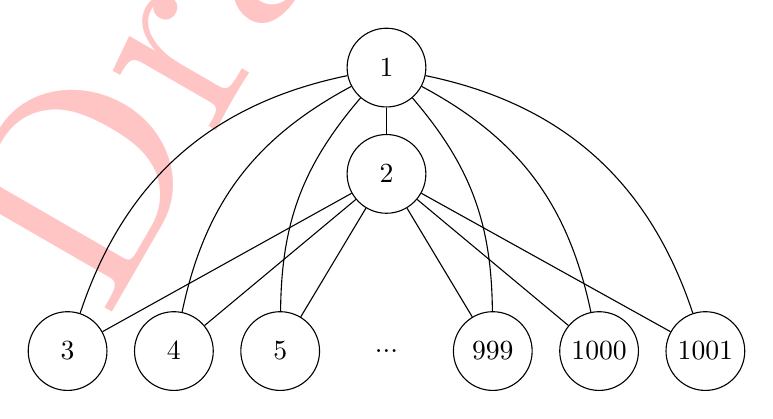
\begin{tikzpicture}[>=latex,scale=0.9]
            \begin{scope}[every node/.style={circle, draw = black,minimum size=10mm,inner sep=2pt}] 
                \node (1) at (0, 0) {1};
                \node (2) at (0, -1.5) {2};
                \node (3) at (-4.5, -4) {3};
                \node (4) at (-3, -4) {4};
                \node (5) at (-1.5, -4) {5};
                \node (7) at (1.5, -4) {999};
                \node (8) at (3, -4) {1000};
                \node (9) at (4.5, -4) {1001};
            \end{scope}
            \tikzset{e4c node/.style={circle,draw=none,minimum size=1.0cm,inner sep=0}}
            \node (6) at (0, -4) {...};
    
            \draw (1)--(2);
            \draw (2)--(3);
            \draw (2)--(4);
            \draw (2)--(5);
            \draw (2)--(7);
            \draw (2)--(8);
            \draw (2)--(9);
    
            \path
                (3) edge[-, bend left = 30] (1)
                (4) edge[-, bend left = 25] (1)
                (5) edge[-, bend left = 20] (1)
                (7) edge[-, bend left = -20] (1)
                (8) edge[-, bend left = -25] (1)
                (9) edge[-, bend left = -30] (1);
        \end{tikzpicture}
        \end{center}
    \end{enumerate}

    % Patryk
    \sol Koszt wykonania algorytmu Dijkstry dla spójnego grafu $n$-wierzchołkowego o $m$ krawędziach wynosi
    \answerss{$O(m\log{n})$ w implementacji z kopcem zupełnym}{$O(n\log{n}+m)$ w implementacji z kopcem Fibonacciego}{$O(n^2)$ w implementacji z kolejką dwumianową}{TAK}{TAK}{NIE}

     Złożoność algorytmu Dijkstry to $O(m\cdot\texttt{DecreaseKey}+n\cdot\texttt{DeleteMin})$. W każdym kopcu operacja \texttt{DeleteMin} ma koszt $O(\log{n})$, podobnie jak \texttt{DecreaseKey}, które jedynie w przypadku kopca Fibonacciego amortyzuje się do czasu stałego.

    \begin{enumerate}[\bf A.]
        \item Czas będzie $O(m\log{n}+n\log{n})$, ale ponieważ graf jest spójny, to ma co najmniej $\Omega(n)$ krawędzi, więc drugi składnik sumy nic nie wnosi do złożoności i odpowiedzią jest \texttt{TAK}.

        \item Wstawiając powyższe złożoności kopca Fibonacciego do wzoru otrzymamy dokładnie taką złożoność, odpowiedź to \texttt{TAK}.

        \item Złożoność jest taka sama jak w \textbf{A.} ($O(m \log n)$), a $m$ może być rzędu $n^2$, więc odpowiedź to \texttt{NIE}.
    \end{enumerate}

    % Jasiek
    \sol Wysokość drzewa ukorzenionego mierzymy liczbą krawędzi na najdłuższej ścieżce z korzenia do wierzchołka w tym drzewie. Dany jest spójny $n$-wierzchołkowy graf dwuspójny wierzchołkowo (tzn. bez wierzchołków rozdzielających) o co najmniej 4 wierzchołkach. Prawdą jest, że
    \answerss{wysokość każdego drzewa przeszukiwania wszerz w takim grafie jest mniejsza od $n / 2$}{wysokość każdego drzewa przeszukiwania w głąb w takim grafie jest większa od $n / 2$}{wysokość każdego drzewa przeszukiwania w głąb w takim grafie wynosi co najmniej $3$}{NIE}{NIE}{NIE}
    
    Kontrprzykładem w \textbf{A.} może być cykl 4-wierzchołkowy. W takim cyklu głębokość drzewa BFS jest równa $2 = \frac{n}{2}$ (niezależnie od wierzchołka startowego).
    
    Kontrprzykład do \textbf{B.} oraz \textbf{C.} narysowany jest poniżej (wierzchołek o numerze 1 jest korzeniem w drzewie, a DFS wchodzi najpierw do wierzchołka numer 2):
    \begin{center}
        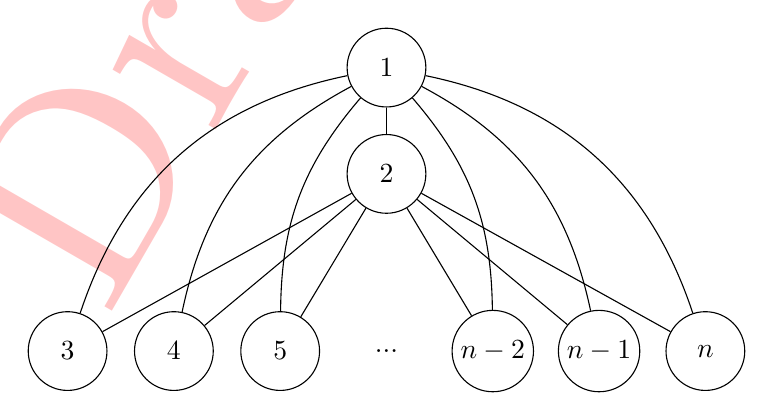
\begin{tikzpicture}[>=latex,scale=0.9]
            \begin{scope}[every node/.style={circle, draw = black,minimum size=10mm,inner sep=2pt}] 
                \node (1) at (0, 0) {1};
                \node (2) at (0, -1.5) {2};
                \node (3) at (-4.5, -4) {3};
                \node (4) at (-3, -4) {4};
                \node (5) at (-1.5, -4) {5};
                \node (7) at (1.5, -4) {$n - 2$};
                \node (8) at (3, -4) {$n - 1$};
                \node (9) at (4.5, -4) {$n$};
            \end{scope}
            \tikzset{e4c node/.style={circle,draw=none,minimum size=1.0cm,inner sep=0}}
            \node (6) at (0, -4) {...};
    
            \draw (1)--(2);
            \draw (2)--(3);
            \draw (2)--(4);
            \draw (2)--(5);
            \draw (2)--(7);
            \draw (2)--(8);
            \draw (2)--(9);
    
            \path
                (3) edge[-, bend left = 30] (1)
                (4) edge[-, bend left = 25] (1)
                (5) edge[-, bend left = 20] (1)
                (7) edge[-, bend left = -20] (1)
                (8) edge[-, bend left = -25] (1)
                (9) edge[-, bend left = -30] (1);
        \end{tikzpicture}
    \end{center}

    % Julia
    \sol Wysokość drzewa BST zawierającego 100 wierzchołków
    \answerss{wynosi co najmniej 49}{wynosi co najmniej 7}{wynosi co najwyżej 99}{NIE}{NIE}{TAK}

    Drzewo BST o największej wysokości to prosta z naniesionymi kolejnymi wierzchołkami, zatem wysokość takiego drzewa jest równa liczbie wierzchołków pomniejszonej o jeden (w naszym przypadku $99$).
    
    Drzewo BST z najmniejszą liczbą wierzchołków, to drzewo, w którym wierzchołki na każdym poziomie (oprócz ostatniego) mają po dwóch synów. Zatem wysokość takiego drzewa będzie wynosiła $\lfloor \log_2(n) \rfloor$, gdzie $n$ to liczba wierzchołków (w naszym przypadku $6$).

    % Julia
    \sol O drzewach AVL prawdą jest, że
    \answerss{największe drzewo AVL o wysokości 5 ma 64 wierzchołki}{najmniejsze drzewo AVL o wysokości 5 ma 20 wierzchołków}{każde drzewo czerwono-czarne jest AVL drzewem}{NIE}{TAK}{NIE}

    \begin{enumerate}[\bf A.]
        \item Największe drzewo AVL to po prostu największe drzewo BST, czyli drzewo posiadające dwóch synów na każdym poziomie. Zatem największe drzewo AVL o wysokości $h$ będzie posiadać $2^{h+1} - 1$ wierzchołków (czyli w naszym przypadku 63).

        \item Rozwiązanie tego podpunktu dość łatwo narysować na kartce, dokładając kolejno potrzebne wierzchołki. Można też skorzystać ze wzoru $M(h) = 1 + M(h-1) + M(h-2)$, gdzie $M(h)$ to minimalna liczba wierzchołków w drzewie AVL o wysokości $h$.

        \item Nie, ponieważ drzewo czerwono-czarne nie musi być zbalansowane, tak jak drzewo AVL.
    \end{enumerate}

    % Patryk
    \sol Do początkowo pustego drzewa BST wstawiamy kolejno elementy pewnej permutacji liczb $1,2,\ldots,16$. Liczba permutacji, dla których
    \answerss{dostaniemy drzewo o wysokości (czyli maksymalnej liczbie krawędzi na ścieżce od korzenia do liścia) równej 15, wynosi co najwyżej $2^{16}$}{dostaniemy drzewo o wysokości równej 3, wynosi co najmniej $2^{15}$}{w lewym poddrzewie korzenia będzie tylko węzeł z kluczem 1, wynosi co najmniej jeden miliard}{TAK}{NIE}{TAK}

    \begin{enumerate}[\bf A.]
        \item Żeby zbudować drzewo o takiej (maksymalnej) wysokości, w permutacji muszą występować kolejno największa lub najmniejsza aktualnie możliwa liczba, np. $16,1,2,3,15,4,14,13,12,5,6,11,...$. Na każdym kroku mamy wybór pomiędzy dwoma liczbami, więc takich permutacji będzie $2^{15} \leq 2^{16}$.

        \item Drzewo o wysokości 3 może mieć maksymalnie 15 elementów, więc jest 0 takich permutacji.

        \item Aby w lewym poddrzewie była tylko jedynka, pierwszym elementem permutacji musi być ,,2'', reszta może być losowo. Zatem takich permutacji jest $15!$. Wiemy że $7! > 1000 = 10^3$ oraz $15\cdot 14\cdot 13\cdot 12\cdot 11\cdot 10\cdot > 10^6$ więc $15! > 10^9$.
    \end{enumerate}

    % Grześ
    \sol W zbiorze AVL-drzew o 10 węzłach
    \answerss{istnieje drzewo o wysokości (czyli największej liczbie krawędzi od korzenia do liścia) równej 4}{każde drzewo ma wysokość co najmniej 3}{maksymalna różnica liczb węzłów poddrzew korzenia wynosi 5}{NIE}{TAK}{TAK}

    \begin{enumerate}[\bf A.]
        \item Minimalna liczba wierzchołków w AVL drzewie o wysokości 4 wynosi 12, więc mając 10 wierzchołków możemy uzyskać co najwyżej wysokość 3.

        \item Pełne drzewo binarne o wysokości 2 ma 7 wierzchołków, więc mając ich 10 możemy zbudować drzewo co najmniej o wysokości równej 3.

        \item Maksymalną różnicę dostaniemy, jeśli jednym poddrzewem korzenia będzie wierzchołek mający jednego syna, który jest liściem, a drugie poddrzewo korzenia będzie pełnym drzewem binarnym o wysokości równej 2. Wtedy lewe poddrzewo ma 2 wierzchołki, a prawe -- 7.
    \end{enumerate}

    \sol Niech $\Sigma = \{a, b\} $ będzie dwuznakowym alfabetem, a $s$ i $t$ słowami nad $\Sigma$ o długościach odpowiednio $m$ i $n$, gdzie $0 < m \leq n$. W algorytmie KMP wyszukiwania wzorca $s$ w tekście $t$
    \answerss
    {wszystkie wystąpienia słowa $s$ w słowie $t$ zostaną znalezione w czasie $O(n)$}
    {preprocessing zajmuje czas $\Omega (n)$}
    {każdy symbol ze słowa $t$ jest porównywany z co najwyżej jednym symbolem ze słowa $s$}
    {TAK}{TAK}{NIE}
    \textbf{A.} Algorytm KMP działa w czasie $O(n)$.

    \textbf{B.} Trzeba policzyć tablicę prefikso-sufiksów, co zajmuje czas liniowy.

    \textbf{C.} Nie musi tak być, np. mając $s=abab$ i $t=ababab$, prefikso-sufiks słowa $s$ wynosi 2, więc po każdym wystąpieniu wzorca w tekście cofniemy się o 2, więc niektóre symbole z $t$ porównamy dwa razy.

% COTO
    % Grześ
    \sol Dana jest funkcja
    \begin{cpp}
        int coto(int n) {
            if (n = 0)
                return 1;
            else if (n > 0)
                return coto(n - 1) + coto(-n);
            else
                return coto(n + 1) - 1;
        }
    \end{cpp}
    Przypisanie \cppinline{y = coto(x)} spowoduje, że będzie zachodzić zależność
    \answerss{$|y|\geq|x|$}{$y\leq1$}{jeśli $x=-2012$, to $y=-2011$}{NIE}{TAK}{TAK}
    
    Prześledźmy, co robi funkcja \cppinline{coto(x)}. Jeśli $x=0$, to \textbf{wyznacza} wartość 1. Jeśli $x<0$, to funkcja \textbf{oblicza} wartość $|x|\cdot(-1)+1=-|x|+1=x+1$. Jeśli $x>0$, to funkcja \textbf{przekazuje} wartość rekurencji $F_n=F_{n-1}-n+1$. Ostatecznie,
    $$
    \cppinline{coto(x)}=\begin{cases}
        1 & \text{gdy } x=0 \\
        \cppinline{coto(x-1)}-x+1 & \text{gdy } x>0 \\
        x+1 & \text{gdy } x<0
    \end{cases}=\begin{cases}
        \cppinline{coto(x-1)}-x+1 & \text{gdy } x>0 \\
        x+1 & \text{wpp.}
    \end{cases}
    $$

    \begin{enumerate}[\bf A.]
        \item Widzimy, że wstawiając za $x$ ujemną liczbę (np. $-5$) dostaniemy w wyniku liczbę większą o 1 (np. $-4$), czyli w module będzie to liczba mniejsza o 1, a więc fałsz.

        \item Dla liczb niedodatnich widać od razu. Dla liczb dodatnich można by policzyć tą rekurencję, ale można też rozpisać kilka pierwszych wyrazów ciągu: $(1,0,-2,-5,-9,\ldots)$. Już dla $x>2$ dostajemy liczby ujemne, a dla $x=0$ i $x=1$ coś nie większego od 1, czyli odpowiedź to \texttt{TAK}

        \item Widać od razu -- dla liczby ujemnej dostajemy liczbę większą o 1.
    \end{enumerate}

    PS. \textit{Istnieje w języku polskim niezbyt szczęśliwe tłumaczenie słowa ,,return'', jako ,,zwracać''. Jest to niezbyt zręczna kalka językowa bez specjalnego uzasadnienia. Zamiast mówić ,,funkcja zwraca wartość'' proponuję ,,funkcja \{wyznacza, oblicza, przekazuje\} wartość''.} Autor rozwiązania trzymał się konwencji poznanej na Wstępie do Programowania Imperatywnego autorstwa docenta Piotra Chrząstowskiego-Wachtla i zachęca, aby Czytelnik również się do niej stosował.
\end{solutions}


\chapter{Języki, automaty i obliczenia}

Materiały teoretyczne z tego przedmiotu zostały opracowane na podstawie \href{https://www.mimuw.edu.pl/~szymtor/jao/skrypt.pdf}{skryptu Szymona Toruńczyka}.

\section*{Podstawa programowa}
\begin{enumerate}
    \item \textbf{Języki regularne}, wyrażenia regularne, automaty skończone.
    \item \textbf{Języki bezkontekstowe}, gramatyki bezkontekstowe, automaty ze stosem.
    \item \textbf{Lematy o pompowaniu} dla języków regularnych i bezkontekstowych.
    \item \textbf{Języki obliczalne} i częściowo obliczalne. Problem stopu oraz metoda przekątniowa.
    \item \textbf{Klasy P, NP} oraz NP-zupełność.
\end{enumerate}

% Filip
\section{Języki regularne}

\textbf{Automat niedeterministyczny (NFA)} to krotka $\langle A, Q, I, F, \delta \rangle$, gdzie:

\begin{itemize}
    \item $A$ to alfabet, czyli skończony zbiór symboli zwanych dalej \textit{literami},
    \item $Q$ to skończony zbiór stanów,
    \item $I \subseteq Q$ to zbiór stanów początkowych,
    \item $F \subseteq Q$ to zbiór stanów akceptujących,
    \item $\delta \subseteq Q \times A \times Q$ to relacja przejścia.
\end{itemize}

\textbf{Automat deterministyczny (DFA)} to prawie taka sama krotka $\langle A, Q, I, F, \delta \rangle$ jak powyżej, ale z tą różnicą, że $\delta$ to funkcja typu $Q \times A \to Q$, a nie tylko relacja.

\textbf{Automat z $\epsilon$-przejściami} to automat dopuszczający przejścia postaci $(p, \epsilon, q)$, gdzie $\epsilon$ to słowo puste.

Terminologia:
\begin{itemize}
    \item \textit{tranzycja (przejście)} -- trójka $(p, a, q) \in \delta$, również oznaczana jako $p \xrightarrow{a} q$,
    \item \textit{bieg} -- ciąg tranzycji $q_0 \xrightarrow{a_1} q_1 \xrightarrow{a_2} q_2 \xrightarrow{a_3} \ldots \xrightarrow{a_n} q_n$, gdzie $q_0 \in I$ i który można interpretować jako ścieżkę w grafie automatu,
    \item \textit{bieg akceptujący} -- bieg, który kończy w stanie akceptującym,
    \item \textit{bieg po słowie $w$} -- bieg $q_0 \xrightarrow{a_1} q_1 \xrightarrow{a_2} q_2 \xrightarrow{a_3} \ldots \xrightarrow{a_n} q_n$ taki, że $a_1 a_2 a_3 \ldots a_n = w$.
    \item automat $\mathcal{A}$ \textit{akceptuje} słowo $w \in A^*$, jeżeli istnieje bieg akceptujący po tym słowie,
    \item automat $\mathcal{A}$ \textit{rozpoznaje} język $L$, jeśli $w \in L \wtw \mathcal{A}$ akceptuje $w$ i oznaczamy to jako $L = \mathcal{L}(A)$.
\end{itemize}

\textbf{Wyrażenie regularne} to wyrażenie zbudowane rekurencyjnie, które reprezentuje pewien język. Tak samo jak dla automatów, dla wyrażenia regularnego $A$ reprezentującego język $L$ piszemy, że $L = \mathcal{L}(A)$. Można je budować przy pomocy następujących reguł:
\begin{itemize}
    \item $\emptyset$ jest wyrażeniem regularnym reprezentującym język pusty,
    \item $a$ jest wyrażeniem regularnym reprezentującym język $A = \{ a \}$,
    \item dla wyrażeń $A, B$: $A + B$ reprezentuje język $\mathcal{L}(A) \cup \mathcal{L}(B)$,
    \item dla wyrażeń $A, B$: $A \cdot B$ (lub po prostu $AB$) reprezentuje język $K \cdot L = \{ v \cdot w \mid v \in K, w \in L \}$, gdzie $K = \mathcal{L}(A), L = \mathcal{L}(B)$,
    \item dla wyrażenia $A$: $A^*$ reprezentuje język $\{ w_1 \cdot w_2 \cdot \ldots \cdot w_n \mid w_1, w_2, \ldots, w_n \in \mathcal{L}(A), n \in \mathbb{N} \}$.
\end{itemize}

Prawdziwy jest następujący \textbf{lemat o równoważności automatów i wyrażeń regularnych}: niech $L \subseteq A^*$. Następujące warunki są równoważne:
\begin{itemize}
    \item język $L$ jest reprezentowany przez pewne wyrażenie regularne,
    \item język $L$ jest rozpoznawany przez pewien automat niedeterministyczny,
    \item język $L$ jest rozpoznawany przez pewien automat deterministyczny,
    \item język $L$ jest rozpoznawany przez pewien automat (nie)deterministyczny z $\epsilon$-przejściami.
\end{itemize}

Języki regularne są zamknięte na:
\begin{itemize}
    \item \textbf{sumę} -- dla języków regularnych $K$ i $L$, język 
    $K \cup L$ jest regularny.
    \item \textbf{konkatenację} -- dla języków regularnych $K$ i $L$, język $K \cdot L = \{ w_K \cdot w_L : w_K \in K, w_L \in L \}$ jest regularny.
    \item \textbf{gwiazdkę Kleene'ego} -- dla języka regularnego $L$,
    język $L^* = \{ w_1 \cdot w_2 \cdot \ldots \cdot w_n : w_1, w_2, \ldots, w_n \in L,
    n \in \mathbb{N} \}$
    jest regularny.
    \item \textbf{przecięcie} -- dla języków regularnych $K$ i $L$, język $K \cap L$ jest regularny.
    \item \textbf{dopełnienie} -- dla języków regularnych $K$ i $L$, język $K - L$ jest regularny.
    \item \textbf{odwrócenie języka} -- Dla języka regularnego $L$, język $L^R = \{w^R \mid w \in L\}$ jest regularny.
\end{itemize}

\subsection{Minimalizacja automatów}
Ponieważ wiele automatów może rozpoznawać ten sam język regularny, możemy rozważać \textbf{problem minimalizacji} -- jaka jest najmniejsza liczba stanów, jaką musi posiadać automat, żeby rozpoznawał dany język? Rozważany automat będzie automatem \textit{deterministycznym} i będzie nazywany \textit{automatem syntaktycznym}. Do znalezienia takiego automatu przydatna będzie relacja Myhilla-Nerodego:
\[
u \sim_L v \wtw \forall w \in A^* \ : \ (uw \in L \wtw vw \in L)
\]

Możemy interpretować tę relację następująco: słowa $u, v$ są w relacji jeśli mają tę samą ,,przyszłość'' -- zaczynając od wczytania $u$, wczytywanie dalszych liter doprowadza nas do tego samego rezultatu, jak gdybyśmy zaczęli od $v$. Relację tę z problemem minimalizacji łączy twierdzenie:

Jeśli język $L$ ma skończenie wiele klas abstrakcji w sensie relacji Myhilla-Nerodego, to jest językiem regularnym. Ponadto, automat syntaktyczny dla tego języka posiada dokładnie tyle stanów, ile było klas abstrakcji.

\begin{example}
Znajdziemy liczbę stanów automatu syntaktycznego rozpoznającego język $L = aa^*b^*$. W tym celu znajdziemy wszystkie klasy abstrakcji relacji Myhilla-Nerodego nad tym językiem. Pierwszą klasą abstrakcji będzie $[\epsilon]$. Metodą prób i błędów znajdziemy następne klasy abstrakcji.

Rozpatrzmy $[a]$ i sprawdźmy, czy jest to klasa abstrakcji różna od $[\epsilon]$. Musimy znaleźć słowo $w$, które jest różnymi ,,przyszłościami'' dla $a$ i $\epsilon$ -- czyli takie, że tylko jedno ze słów $aw$ i $\epsilon w = w$ należy do $L$. Łatwo zauważyć, że działa $w = \epsilon$. Zatem $[a] \not= [\epsilon]$. 

Spróbujemy znaleźć następną klasę. Rozpatrzmy $[b]$. Zauważmy, że jeśli na początek wczytamy $b$, to ,,nie mamy przyszłości'' -- nieważne co wczytamy dalej, nie osiągniemy akceptacji. Łatwo widać, że jest to klasa różna od poprzednich.

Ostatnią klasą abstrakcji będzie $[ab]$ -- po wczytaniu słowa $ab$, aby dostać akceptację możemy wczytywać już tylko same litery $b$, co nie było prawdą dla poprzednich klas.

Możemy próbować szukać następnych klas, ale okazywać się będzie, że są równe znalezionym już przez nas klasom. Aby się upewnić, można narysować automat języka $L$, kładąc klasy abstrakcji jako stany:

\begin{center}
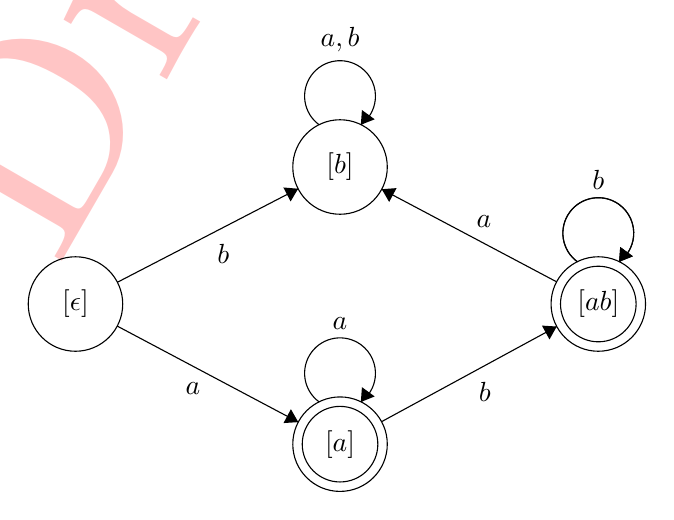
\begin{tikzpicture}[scale=0.2]
\tikzstyle{every node}+=[inner sep=0pt]
\draw [black] (24.4,-28.8) circle (3);
\draw (24.4,-28.8) node {$[\epsilon]$};
\draw [black] (41.2,-20.1) circle (3);
\draw (41.2,-20.1) node {$[b]$};
\draw [black] (41.2,-37.7) circle (3);
\draw (41.2,-37.7) node {$[a]$};
\draw [black] (41.2,-37.7) circle (2.4);
\draw [black] (57.6,-28.8) circle (3);
\draw (57.6,-28.8) node {$[ab]$};
\draw [black] (57.6,-28.8) circle (2.4);
\draw [black] (27.05,-30.2) -- (38.55,-36.3);
\fill [black] (38.55,-36.3) -- (38.08,-35.48) -- (37.61,-36.36);
\draw (31.86,-33.75) node [below] {$a$};
\draw [black] (27.06,-27.42) -- (38.54,-21.48);
\fill [black] (38.54,-21.48) -- (37.6,-21.4) -- (38.06,-22.29);
\draw (33.79,-24.95) node [below] {$b$};
\draw [black] (39.877,-17.42) arc (234:-54:2.25);
\draw (41.2,-12.85) node [above] {$a,b$};
\fill [black] (42.52,-17.42) -- (43.4,-17.07) -- (42.59,-16.48);
\draw [black] (43.84,-36.27) -- (54.96,-30.23);
\fill [black] (54.96,-30.23) -- (54.02,-30.17) -- (54.5,-31.05);
\draw (50.4,-33.75) node [below] {$b$};
\draw [black] (39.877,-35.02) arc (234:-54:2.25);
\draw (41.2,-30.45) node [above] {$a$};
\fill [black] (42.52,-35.02) -- (43.4,-34.67) -- (42.59,-34.08);
\draw [black] (56.277,-26.12) arc (234:-54:2.25);
\draw (57.6,-21.55) node [above] {$b$};
\fill [black] (58.92,-26.12) -- (59.8,-25.77) -- (58.99,-25.18);
\draw [black] (56.277,-26.12) arc (234:-54:2.25);
\fill [black] (58.92,-26.12) -- (59.8,-25.77) -- (58.99,-25.18);
\draw [black] (54.95,-27.39) -- (43.85,-21.51);
\fill [black] (43.85,-21.51) -- (44.32,-22.32) -- (44.79,-21.44);
\draw (50.34,-23.95) node [above] {$a$};
\end{tikzpicture}
\end{center}


Rzeczywiście, jest to automat deterministyczny rozpoznający powyższy język. Zatem minimalny automat ma 4 stany.
\end{example}

\subsection{Lemat o pompowaniu dla języków regularnych}

Przypuśćmy, że język $L \subseteq A^*$ jest regularny. Wówczas istnieje taka stała 
$N \in \mathbb{N}$, że dla każdego słowa $w \in L$ długości co najmniej $N$ istnieje
dekompozycja $w = w_1 \cdot w_2 \cdot w_3$ o następujących własnościach:
\begin{itemize}
    \item słowo $w_2$ jest niepuste,
    \item $|w_1 \cdot w_2| \leq N$,
    \item dla dowolnej liczby naturalnej $k \geq 0$ słowo $w_1 \cdot w_2^k \cdot w_3$
    należy do języka $L$.
\end{itemize}

\begin{example} 
    Pokażemy, że język $L = \{ a^nb^n \mid n \geq 0 \}$ nie jest regularny.
    Przypuśćmy przeciwnie. Wówczas istnieje stała $N \in \mathbb{N}$, 
    o której mowa w lemacie o pompowaniu. Rozważmy słowo $w = a^N b^N$. 
    To słowo należy do języka $L$, więc istnieje dekompozycja $w = w_1 \cdot w_2 \cdot w_3$,
    taka, że $w_2 \neq \epsilon$, $w_1 \cdot w_2^k \cdot w_3 \in L$ dla $k \geq 0$,
    oraz $|w_1 \cdot w_2| \leq N$. Wynika stąd, że słowo $w_2$ zawiera wyłącznie litery $a$
    oraz jest niepuste. Słowo $w_1 \cdot w_2 \cdot w_3$ zawiera więcej liter $a$ niż liter $b$,
    więc nie należy do języka $L$, co jest sprzecznością. Otrzymana sprzeczność pokazuje, że język
    $L$ nie jest regularny.
\end{example}

\begin{problems}
\prob Rozważmy wyrażenie regularne $K=A^* bb A^* + A^* a A A + A^* a A$ nad alfabetem $\{a,b\}$ (zapis $A$ w wyrażeniu to skrót na $(a + b)$). Niech $L$ to język tego wyrażenia. Wtedy
    \answers{automat minimalny dla $L$ ma co najwyżej $4$ stany}{automat minimalny dla $L$ ma przynajmniej $6$ stanów}{istnieje automat niedeterministyczny dla $L$ o $5$ stanach}
    
\prob Dany jest język regularny $L$ dany wyrażeniem regularnym $(a+b)^*a(a+b)(a+b)$. Wówczas
    \answers{każdy automat deterministyczny rozpoznający $L$ ma co najmniej 9 stanów}{minimalny automat deterministyczny rozpoznający $L$ ma 7 stanów}{każdy automat niedeterministyczny rozpoznający $L$ ma co najmniej 6 stanów}
    
\prob Regularny jest język nad alfabetem $\{a,b\}$ złożony ze wszystkich słów, w których każde podsłowo
    \answers{długości 3 występuje parzystą liczbę razy}{długości większej niż 3 występuje parzystą liczbę razy}{występuje również jako prefiks}
\prob Regularny jest język złożony ze wszystkich słów nad alfabetem $\{a,b,c\}$, które
    \answers{zaczynają się od $baca$}{nie zawierają $baca$ jako podsłowa}{zawierają $baca$ jako podsłowo parzystą liczbę razy}   
    
\prob $L$ jest regularny. Czy regularny jest:
    \answers{$\{w: w \in L \land w \in L^R\}$}{$\{ww: w \in L\}$}{prefiksy słów z $L$ parzystej długości}

\prob Językiem regularnym jest
    \answers{język $L \subseteq \{1\}^*$ składający się z unarnych reprezentacji liczb pierwszych}{język $L \subseteq \{0, 1\}^*$ składający się ze słów, w których liczba wystąpień cyfry $0$ przystaje modulo $2$ do liczby wystąpień cyfry $1$}{język $L \subseteq \{0, 1\}^*$ składający się z binarnych reprezentacji liczb podzielnych przez $7$}
\end{problems}

% Michał
\section{Języki bezkontekstowe}
\textbf{Gramatyka bezkontekstowa} $\mathcal{G}$ ma następujące składniki:
\begin{itemize}
    \item Zbiór \textit{terminali} $A$,
    \item Zbiór \textit{nieterminali} $N$, rozłączny z $A$,
    \item Zbiór \textit{produkcji} postaci $q \to w$, gdzie $q \in N$ oraz $w \in (A \cup N)^*$
    jest słowem składającym się z terminali i/lub nieterminali.
    \item Symbolu \textit{startowego} $S$
\end{itemize}

\textbf{Drzewem parsowania} takiej gramatyki jest drzewo etykietowane, w którym:
\begin{itemize}
    \item etykieta korzenia to symbol startowy $S$
    \item liście etykietowane są terminalami ze zbioru $A \cup \{ \epsilon \}$,
    \item wierzchołki wewnętrzne etykietowane są nieterminalami ze zbioru $N$,
    \item jeżeli wierzchołek wewnętrzny ma etykietę $q$, to ma $k$ dzieci o etykietach $s_1, \dots, s_k \in (N \cup A)$ (czytając od lewej do prawej) oraz $q \to s_1 s_2 \dots s_k$ jest produkcją gramatyki (wyjątek: zamiast $k = 0$ robimy dziecko o etykiecie $\epsilon$)
\end{itemize}

\textit{Plon drzewa} to słowo utworzone z etykiet liści, czytanych od lewej do prawej.

\begin{example}
    Rozważmy gramatykę $\mathcal{G}$  o terminalach $a$ oraz $b$, nieterminalu $S$ oraz produkcjach
    $$S \to aSa \; | \; bSb \; | \; a \; | \; b \; | \; \epsilon$$

    Drzewo parsowania dla słowa $abbba$:
    \begin{center}
    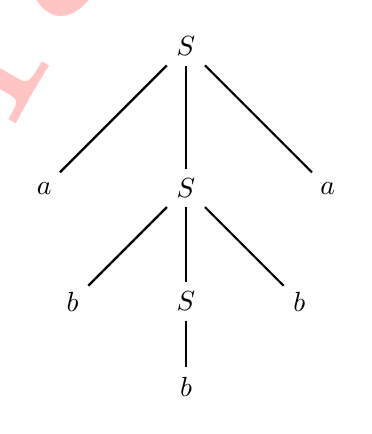
\begin{tikzpicture}[x=1.8cm,y=1.8cm]
        \node (1) at (1.0, 5.0) {$S$}; 
        \node (2) at (0.0, 4.0) {$a$}; 
        \node (3) at (1.0, 4.0) {$S$}; 
        \node (4) at (2.0, 4.0) {$a$}; 
        \node (5) at (0.2, 3.2) {$b$};
        \node (6) at (1.0, 3.2) {$S$};
        \node (7) at (1.8, 3.2) {$b$};
        \node (8) at (1.0, 2.6) {$b$};
        
        \path[-,draw,thick]
            (1) edge (2)
            (1) edge (3)
            (1) edge (4)
            (3) edge (5)
            (3) edge (6)
            (3) edge (7)
            (6) edge (8)
        ;
    \end{tikzpicture}
    \end{center}
    
    Przez indukcję po rozmiarze drzewa parsowania widać, że plonem każdego drzewa parsowania jest palindrom, tj. takie słowo $w$, że $w = w^R$. Odwrotna inkluzja również zachodzi, co możemy udowodnić (ponownie przez indukcję) konstruując drzewo parsowania dla każdego palindromu. Tak więc, $L(\mathcal{G})$ to język palindromów nad alfabetem $\{a, b\}$.
\end{example}

\begin{lemma}
    Każdy język regularny jest bezkontekstowy.
\end{lemma}
Szkic dowodu: dla każdego automatu, da się skonstruować gramatykę, która mu odpowiada.

\subsection{Lemat o pompowaniu dla języków bezkontekstowych}
\begin{lemma} 
    Przypuśćmy, że język $L \subseteq A^*$ jest bezkontekstowy.
    Wtedy istnieje takie $N \in \mathbb{N}$, że każde
    słowo $w \in L$ długości co najmniej $N$ posiada 
    faktoryzację
    $$w = prefix \cdot left \cdot infix \cdot right \cdot suffix$$
    o następujących własnościach:
    \begin{itemize}
        \item słowo $left \cdot right$ jest niepuste
        \item słowo $left \cdot infix \cdot right$
        ma długość co najwyżej $N$
        \item dla każdego $k \geq 0$ słowo
        $w_k = prefix \cdot left^k \cdot infix \cdot right^k \cdot suffix$ należy do języka $L$.
    \end{itemize}
\end{lemma}

\begin{example}
    Pokażemy, że język $L = \{ a^n b^n c^n \mid n \geq 0 \} \subseteq \{a, b, c\}^n$
    nie jest bezkontekstowy. Przypuśćmy przeciwnie. Wtedy istnieje stała $N \in \mathbb{N}$ o której mowa w lemacie o pompowaniu. 
    Rozważmy słowo $w = a^N b^N c^N$ i jego faktoryzację.
    Gdyby $left$ zawierał dwie różne litery 
    (tj. $a$ i $b$, lub $a$ i $c$, lub $b$ i $c$), to słowo $w_2$ nie mogłoby
    należeć do języka $L$. Zatem, $left$ używa tylko jednej litery i analogicznie $right$. 
    Zatem jedna z liter $a$, $b$, $c$, nazwijmy ją $x$, 
    nie pojawia się ani w słowie $left$, ani w słowie $right$. 
    Ponieważ przynajmniej jedno ze słów $left$, $right$ jest niepuste, 
    to jakaś litera $y$ różna od $x$ pojawia się w $left$ lub $right$. 
    Słowo $w_2$ ma więc więcej wystąpień litery $y$ niż litery $x$, 
    więc $w_2 \notin L$. To przeczy tezie lematu o pompowaniu. Tak
    więc, język L nie jest bezkontekstowy.

    Zauważmy, że język $L$ jest przecięciem dwóch języków bezkontekstowych:
    $\{ a^n b^n c^m : n, m \geq 0 \}$ oraz 
    $\{ a^n b^m c^m : n, m \geq 0 \}$
    To przykład na to, że języki bezkontekstowe nie są zamknięte na przecięcia,
    a w konsekwencji nie są też zamknięte na dopełnienie.
\end{example}

Języki bezkontekstowe są zamknięte na:
\begin{itemize}
    \item sumę, konkatenację, gwiazdkę Kleene'go, odwrócenie,
    \item przecięcia z językami regularnymi -- jeśli $L$ jest językiem bezkontekstowym, a $K$ jest językiem regularnym,
    to $L \cap K$ jest językiem bezkontekstowym.
\end{itemize}

% Filip
\subsection{Automaty ze stosem}
Języki bezkontekstowe są rozpoznawane przez pewien rodzaj automatów, nazywanych \textit{automatami ze stosem}. Są one uogólnieniem NFA z $\epsilon$-przejściami, ale z dodatkowym \textit{stosem}. Automat taki ma następujące składniki:
\begin{itemize}
    \item Alfabet wejściowy $A$,
    \item Alfabet stosowy $\Gamma$ zawierający symbol \ dna stosu,
    \item Zbiór stanów $Q$,
    \item Zbiór stanów początkowych $I \subseteq Q$,
    \item Zbiór stanów akceptujących $F \subseteq Q$,
    \item Zbiór przejść $\delta$, gdzie każde jest postaci:
    \[
    p \xrightarrow{ \textbf{pop}(Z),a,\textbf{push}(\gamma) } q
    \]
    dla pewnych $p,q \in Q$, $a \in A \cup \{\epsilon\}$, $Z \in \Gamma$, $\gamma \in \Gamma^*$.
\end{itemize}

Oczywiście \textbf{pop($Z$)} usuwa literę $Z$ z góry stosu, zaś \textbf{push($\gamma$)} wrzuca na stos słowo $\gamma$ (zakładamy, że wrzucenie całego słowa na stos działa tak samo jak wrzucanie po kolei liter od pierwszej do ostatniej -- innymi słowy, stos rośnie w prawo i \textbf{push} dokleja słowo do stosu).

Ważne fakty o automatach ze stosem:
\begin{itemize}
    \item Automaty ze stosem mają tę samą siłę wyrazu co języki bezkonstekstowe,
    \item Zamiast rozważać stany akceptujące można rozważać model, w którym akceptacja zachodzi wtedy, gdy stos jest pusty -- te dwa modele są równoważne,
    \item Każdy automat ze stosem można przerobić na równoważny, mający tylko jeden stan i akceptujący poprzez pusty stos.
\end{itemize}

\begin{problems}

\prob Załóżmy, że $L$ to język bezkontekstowy, zaś $K$ to język regularny, oba nad alfabetem $A$. Przez $X^R$ oznaczamy język powstały z $X$ przez odwrócenie wszystkich słow z $X$. Językiem bezkontekstowym jest język
    \answers{$L^R \cap K$}{$(A^{*} - L) \cup K^*$}{$L^{*} \cup K^R$}

\prob Dane są język bezkontekstowy $L$ i język regularny $K$. Prawdą jest, że
    \answers{$K \backslash L$ jest bezkontekstowy}{$K \cap L$ jest regularny}{$L \backslash K$ jest bezkontekstowy}

\prob Niech $L$ będzie nieskończonym językiem bezkontekstowym nad skończonym alfabetem. Wówczas
    \answers{$L$ jest regularny}{$L$ zawiera nieskończony język regularny}{$L$ zawiera słowo postaci $uv^{2020}xy^{2020}z$, gdzie $vy \neq \epsilon$}

\prob Niech $L$, $K$ to języki bezkontekstowe. Bezkontekstowy wtedy też jest język
    \answers{$L \cup K$}{$L \cap K$}{$L \cap a^*b^*$}

\prob Dla języka $L$, niech $\Psi(L)$ oznacza zbiór długości słów z języka $L$. Istnieje taki język bezkontekstowy $L$, dla którego $\Psi(L)$ jest zbiorem
    \answers{liczb naturalnych podzielnych przez 11}{kwadratów liczb naturalnych}{sześcianów liczb naturalnych}

\prob $L_1$ i $L_2$ są językami bezkontekstowymi nad alfabetem $\Sigma$. Wynika z tego, że bezkontekstowy jest język
    \answers{$L_1\cap L_2$}{$\Sigma^*-L_1$}{$L_1\cup L_2$}    
\prob $L$ jest językiem bezkontekstowym. Wynika z tego, że bezkontekstowy jest język
    \answers{$\{v$ : istnieje słowo z $L$, które można otrzymać przez usunięcie parzystej liczby (niekoniecznie kolejnych) liter z $v\}$}{$\{ww : w \in L\}$}{$\{a_1 \cdots a_n : a_n \cdots a_1 \in L\}$ (tzn. słowa z $L$ pisane do tyłu)}
    
\prob Następujący język jest bezkontekstowy:
    \answers
    {$\{a^nb^mc^kd^l : n = k \text{ i } m = l\}$}
    {$\{a^nb^mc^kd^l : n = l \text{ i } m = k\}$}
    {$\{a^nb^mc^kd^l :n=m \text{ i } k=l\}$}
    
\prob Jeśli $L_1$ jest językiem bezkontekstowym, a $L_2$ jest językiem regularnym, to bezkontekstowy jest język
    \answers
    {$L_1 \cap L_2$}
    {$\{vw : v \in L_1, w \in L_2\}$}
    {$\{v^R : v \in L_1\}$, gdzie $v^R$ oznacza odwrócenie słowa $v$}

\prob Zbiór dziesiętnych zapisów liczb podzielnych przez 7 jest
    \answers
    {językiem regularnym}
    {językiem bezkontekstowym}
    {językiem kontekstowym}
\end{problems}

% Jasiek
\section{Języki obliczalne}
\textbf{Maszyna Turinga} to krotka $M = \langle A, B, Q, q_I, q_F, \delta \rangle$, gdzie:
\begin{itemize}
    \item $A$ - alfabet wejściowy
    \item $B$ - alfabet roboczy (taki, którym posługuje się maszyna)
    \item $Q$ - skończony zbiór stanów
    \item $q_I$ - stan początkowy
    \item $q_F$ - stan końcowy
    \item $\delta$ - funkcja przejścia, gdzie $\delta: Q \times B \to B \times \{\xleftarrow{}, \xrightarrow{} \} \times Q$
\end{itemize}
Charakterystyka podstawowej maszyny Turinga:
\begin{itemize}
    \item działa na jednostronnie nieskończonym ciągu komórek nazywanym \textbf{taśmą}
    \item posiada głowicę poruszającą się wzdłuż taśmy
    \item głowica wskazuje na aktualnie rozważaną komórkę taśmy
    \item może wykonać tranzycję $t = (p, a, b, d, q)$ w następujący sposób:
    \begin{itemize}
        \item maszyna znajduje się w stanie $p$
        \item w aktualnie rozważanej komórce znajduje się litera $a$
        \item wykonując tranzycję w miejsce litery $a$ wpisana zostaje litera $b$
        \item głowica zostaje przesunięta w kierunku $d \in \{\xleftarrow{}, \xrightarrow{}\}$
        \item maszyna przechodzi do stanu $q$
    \end{itemize}
\end{itemize}
Intuicyjnie maszyna Turinga $M$ jest w stanie sprawdzać swój aktualny stan i na jego podstawie decydować, co zamierza zrobić dalej, być może zmieniając zawartość taśmy. Po więcej szczegółowych definicji odsyłam do \href{https://www.mimuw.edu.pl/~szymtor/jao/skrypt.pdf#chapter.4}{skryptu}.

\textbf{Równoważne warianty maszyn Turinga:}
\begin{itemize}
    \item zwykła maszyna Turinga opisana powyżej;
    \item maszyna Turinga z binarnym alfabetem roboczym ($B = \{0, 1, \_\}$);
    \item maszyna Turinga z taśmą nieskończoną w obu kierunkach;
    \item maszyna Turinga z wieloma taśmami;
    \item niedeterministyczna maszyna Turinga.
\end{itemize}

\textbf{Funkcje obliczalne:} oznaczmy przez $L(M)$ zbiór słów $w \in A^*$, na których maszyna $M$ terminuje. Oznaczmy przez $f_M(w): A^* \to B^*$ funkcję częściową, która słowu $w \in L(M)$ przyporządkowuje wynik obliczenia $M$ na $w$, a dla pozostałych słów jest nieokreślona. Mówimy, że $M$ oblicza funkcję $f_M$. Funkcja częściowa $f: A^* \to B^*$ jest \textbf{obliczalna} jeśli istnieje maszyna Turinga, która ją oblicza.

\begin{example}
    Rozważmy słowa $w \in \{0, 1\}^*$ reprezentujące grafy. Funkcja $f$ ma za zadanie zwrócić jeden wtedy i tylko wtedy, gdy $w$ jest opisem grafu spójnego. Taka funkcja $f$ jest obliczalna, ponieważ możemy zasymulować na taśmie maszyny Turinga algorytm BFS (zapisując m. in. zbiór odwiedzonych wierzchołków i wykonując odpowiednie przejścia).
\end{example}

Język $L \subseteq A^*$ jest \textbf{obliczalny}, jeżeli jego funkcja charakterystyczna jest obliczalna. Jeżeli język $L$ jest obliczalny, to odpowiadający mu problem decyzyjny jest \textbf{rozstrzygalny}. Innymi słowami problem decyzyjny jest rozstrzygalny jeśli istnieje algorytm, który dla każdego słowa wejściowego $w$ terminuje oraz odpowiada "TAK" lub "NIE" w zależności od tego czy $w \in L$. Przykładem języków obliczalnych są języki regularne oraz bezkontekstowe. Języki obliczalne są zamknięte na:
\begin{itemize}
    \item sumy;
    \item przecięcia;
    \item dopełnienia.
\end{itemize}

Język $L \subseteq A^*$ jest \textbf{częściowo obliczalny}, jeżeli istnieje maszyna Turinga, która terminuje dla wszystkich słów $w \in L$, a dla słów $w' \in A^* - L$ nie terminuje. Jeżeli język $L$ jest częściowo obliczalny, to odpowiadający mu problem decyzyjny jest \textbf{półrozstrzygalny}. Innymi słowami problem decyzyjny jest półrozstrzygalny jeśli istnieje algorytm, który dla każdego słowa wejściowego $w$ odpowiada "TAK" wtedy i tylko wtedy, gdy $w \in L$, a w przeciwnym wypadku się wiesza. Każdy język obliczalny jest też częściowo obliczalny. Języki częściowo obliczalne są zamknięte na:
\begin{itemize}
    \item sumy;
    \item przecięcia.
\end{itemize}

\textbf{Lemat 1.} {\it Język $L \subseteq A^*$ jest obliczalny wtw. gdy $L$ oraz $A^* - L$ są częściowo obliczalne.}

\textbf{Lemat 2.} {\it Języki częściowo obliczalne to dokładnie klasa języków rozpoznawanych przez maszyny Turinga.}

\textbf{Problem stopu} -- inaczej nazywany problemem \textbf{HALT} -- dla danej maszyny Turinga $M$ oraz słowa $w$ stwierdź, czy $M$ terminuje na $w$. Do języka HALT należą więc wszystkie pary $\langle M, w \rangle$ takie, że $M$ terminuje na $w$. Język HALT jest częściowo obliczalny (ale nie jest obliczalny). Dopełnienie języka HALT nie jest częściowo obliczalne.

Przydatnym wariantem powyższego problemu jest problem HALT$_\epsilon$, czyli język maszyn Turinga terminujących na słowie pustym. Nie jest on obliczalny. Aby to udowodnić, wykorzystamy metodę \textbf{redukcji}.

\begin{example}
    Załóżmy, że dana jest maszyna $M$ oraz słowo wejściowe $w$. Niech nowa maszyna $M_w$ działa w następujący sposób: $M_w$ wymazuje swoje wejście zastępując je słowem $w$, a następnie symuluje działanie $M$ na $w$. Maszyna $M_w$ zatrzyma się na słowie pustym wtw. gdy $M$ zatrzyma się na słowie $w$. Zatem
    \begin{itemize}
        \item dla danego kodu $k$ maszyny $M$ oraz słowa $w \in A^*$ istnieje kod $k_w$, że $k \in \text{ HALT} \Leftrightarrow k_w \in \text{ HALT}_\epsilon$
        \item funkcja $(k, w) \to k_w$ jest obliczalna
    \end{itemize}
    Z tego wynika, że HALT$_\epsilon$ nie jest obliczalny.
\end{example}

Formalnie, \textbf{redukcja} problemu $L \subseteq A^*$ do problemu $K \subseteq B^*$ to funkcja $f: A^* \to B^*$ taka, że $\forall w \in A^*$ zachodzi $w \in L \Leftrightarrow f(w) \in K$. Redukcja $f$ jest obliczalna jeżeli $f$ jest obliczalna. Oznacza to w szczególności, że jeżeli istnieje redukcja obliczalna języka $L$ do $K$ oraz $K$ jest obliczalny, to $L$ również jest obliczalny.

Znane problemy nierozstrzygalne:
\begin{itemize}
    \item problem stopu
    \item czy język bezkontekstowy $L$ rozpoznaje każde słowo $w \in A^*$?
    \item czy język bezkontekstowy $L$ zawiera się w języku bezkontekstowym $K$?
\end{itemize}

% Jasiek
\section{Klasy P, NP oraz NP-zupełność}
Język $L$ jest w klasie P jeżeli istnieje \textbf{deterministyczna} maszyna Turinga $M$ oraz wielomian $f: \NN \to \NN$ takie, że:
\begin{itemize}
    \item L(M) = L;
    \item dla każdego słowa $w \in A^*$ maszyna $M$ wykonuje co najwyżej $f(|w|)$ kroków na słowie $w$.
\end{itemize}
Mniej formalnie: $L \in$ P jeżeli istnieje algorytm rozwiązujący problem $L$ w czasie wielomianowym.

Język $L$ jest w klasie NP jeżeli istnieje \textbf{niedeterministyczna} maszyna Turinga $M$ oraz wielomian $f: \NN \to \NN$ takie, że:
\begin{itemize}
    \item L(M) = L;
    \item dla każdego słowa $w \in A^*$, każdy bieg maszyny $M$ po słowie $w$ wykonuje co najwyżej $f(|w|)$ kroków.
\end{itemize}

Oczywiście P $\subseteq$ NP, ale czy NP $\subseteq$ P? Jest to bardzo ważny problem otwarty. Wiemy natomiast, że równoważne są warunki:
\begin{itemize}
    \item P = NP
    \item któryś z problemów z poniższej listy należy do klasy P
    \item każdy z problemów z poniższej listy należy do do klasy P
\end{itemize}

Lista niektórych problemów NP-zupełnych:
\begin{itemize}
    \item CNF-SAT \\
    To problem spełnialności formuł w postaci CNF, a więc koniunkcji wielu klauzul, gdzie klauzula jest alternatywą literałów. Literał to zmienna lub negacja zmiennej.
    \item 3CNF-SAT \\
    Instancja problemu CNF-SAT, w której każda klauzula składa się z maksymalnie trzech literałów.
    \item Ścieżka Hamiltona (analogicznie cykl Hamiltona) \\
    Czy w zadanym grafie istnieje ścieżka, która odwiedza każdy z wierzchołków grafu dokładnie raz?
    \item Problem kliki \\
    Czy dany graf zawiera klikę rozmiaru $k$?
    \item Zbiór niezależny \\
    Czy istnieje zbiór mocy $k$ złożony z wierzchołków zadanego grafu $G$ taki, że żadne dwa wierzchołki nie są połączone krawędzią w $G$?
    \item 3-kolorowanie grafu \\
    Czy da się pokolorować wierzchołki grafu na 3 kolory w taki sposób, że żadna krawędź nie łączy dwóch wierzchołków o tym samym kolorze?
    \item akceptacja pustego słowa \\
    Dana niedeterministyczna maszyna Turinga $M$ oraz liczba $n$, czy $M$ akceptuje słowo puste w co najwyżej $n$ krokach?
\end{itemize}

Aby dowieść, że problem $P$ jest NP-zupełny przeprowadzamy \textbf{redukcję wielomianową} z innego, znanego problemu NP-trudnego:
\begin{enumerate}
    \item Uzasadnij, że $P$ jest w klasie NP.
    \item Zredukuj przy pomocy redukcji wielomianowej znany problem NP-trudny do problemu $P$.
    \item $P$ jest w klasie NP i jest NP-trudny $\implies$ $P$ jest NP-zupełny.
\end{enumerate}

Zauważmy, że problem może być NP-trudny (to znaczy co najmniej tak trudny jak inne problemy NP-trudne) nie będąc NP-zupełnym. Jest tak na przykład z problemem stopu.

\begin{example}
    Założmy, że wiemy, że problem 3-kolorowania grafu (3-KOL) jest NP-trudny. Pokażemy, że problem 3-CNF-SAT jest NP zupełny.
    \begin{enumerate}
        \item 3-CNF-SAT jest w klasie NP, ponieważ możemy niedeterministycznie zgadnąć wartościowanie zmiennych, a następnie w czasie wielomianowym sprawdzić, czy formuła logiczna jest spełniona.
        \item Niech $G = (V, E)$ będzie wejściem dla problemu 3-KOL. Dla każdego $v \in V$ tworzymy zmienną $x_v^i, \; i \in \{1, 2, 3\}$ oznaczającą, że wierzchołek $v$ ma kolor $i$. Oczywiście każdy wierzchołek musi mieć przyporządkowany dokładnie jeden kolor, więc tworzymy klauzule:
        \begin{align*}
            \forall_{v \in V} (x_v^1 \lor x_v^2 \lor x_v^3) \land (\neg x_v^1 \lor \neg x_v^2) \land (\neg x_v^1 \lor \neg x_v^3) \land (\neg x_v^2 \lor \neg x_v^2)
        \end{align*}
        Dodatkowo dla każdej krawędzi chcemy, by kolory incydentnych do niej wierzchołków nie były równe:
        \begin{align*}
            \forall_{e = (v, u) \in E} \forall_{i \in \{1, 2, 3\}} (\neg x_v^i \lor \neg x_u^i)
        \end{align*}
        W ten sposób otrzymujemy formułę $\phi$ w postaci 3-CNF. Gdybyśmy potrafili rozwiązać problem 3-CNF-SAT dla $\phi$, to potrafilibyśmy rozwiązać problem 3-KOL dla $G = (V, E)$ przepisując wartościowanie zmiennych na odpowiednie kolory. Taka redukcja jest \textbf{wielomianowa} - dla każdego wierzchołka i krawędzi oryginalnego grafu wykonujemy wielomianową (stałą) liczbę operacji.
        \item 3-CNF-SAT jest w klasie NP oraz jest NP-trudny, a zatem jest NP-zupełny.
    \end{enumerate}
\end{example}

\begin{problems}
\prob Język $L = \{a^nb^n \mid n \in \mathbb{N}\}$ jest
    \answers{regularny}{bezkontekstowy}{obliczalny w czasie wielomianowym}

\prob Zbiór dziesiętnych zapisów potęg dwójki jest
    \answers{językiem bezkontekstowym}{językiem należącym do klasy P}{językiem należącym do klasy NP}

\prob Zakładamy, że język regularny jest dany jako automat niedeterministyczny, a język bezkontekstowy jako gramatyka bezkontekstowa. Problemem rozstrzygalnym jest stwierdzenie
    \answers{czy dany język bezkontekstowy jest zawarty w danym języku bezkontekstowym}{czy dany język bezkontekstowy jest zawarty w danym języku regularnym}{czy dany język regularny jest zawarty w danym języku bezkontekstowym}

\prob Dla dowolnego języka $L \subseteq A^*$ nad alfabetem $A$ oznaczmy przez $L^R$ zbiór ,,lustrzanych odbić'' słów z $L$. Formalnie: $$\epsilon^R = \epsilon, \quad (wa)^R = a(w^R) \text{ dla } a \in A, w \in A^*, \quad L^R = \{w^R : w \in L\}.$$ Niech $L' = LL^R$ oznacza konkatenację języków $L$ i $L^R$. Wynika z tego, że
    \answers
    {jeżeli $L$ jest regularny, to $L'$ też}
    {jeżeli $L$ jest bezkontekstowy, to $L'$ też}
    {jeżeli $L$ jest rozstrzygalny, to $L'$ też}

\prob Problemem rozstrzygalnym jest stwierdzenie
    \answers
    {czy gramatyka bezkontekstowa generuje język regularny}
    {czy możemy rozpoznać słowo puste na maszynie Turinga $\mathcal{M}$ w mniej niż $n$ kroków}
    {czy deterministyczna maszyna Turinga w $f(n)$ krokach rozpozna wszystkie słowa długości $n$ dla każdego $n$}
    
 \prob Dany jest alfabet $A = \{a, b\}$ oraz
    \begin{itemize}
        \item język bezkontekstowy $K$ nad $A$ dany jako gramatyka,
        \item język regularny $R$ nad $A$ dany jako niedeterministyczny automat.
    \end{itemize}
    Problemem rozstrzygalnym jest
    \answers{określenie niepustości podzbioru $R$ takich słów, dla których liczba liter $a$ jest równa liczbie liter $b$}{sprawdzenie, że $K \subset R$}{sprawdzenie, że $R \subset K$}
    
    \prob Problem stopu dla maszyn Turinga jest
    \answers{w klasie NP}{częściowo rozstrzygalny}{rozstrzygalny}
\end{problems}

\begin{solutions}

    % Filip
    \sol Rozważmy wyrażenie regularne $K=A^* bb A^* + A^* a A A + A^* a A$ nad alfabetem $\{a,b\}$ (zapis $A$ w wyrażeniu to skrót na $(a + b)$). Niech $L$ to język tego wyrażenia. Wtedy
    \answerss{automat minimalny dla $L$ ma co najwyżej $4$ stany}{automat minimalny dla $L$ ma przynajmniej $6$ stanów}{istnieje automat niedeterministyczny dla $L$ o $5$ stanach}{TAK}{NIE}{TAK}

    Znajdziemy klasy abstrakcji przy relacji Myhilla-Nerodego. 
    
    \textit{Uwaga.} Dalej w rozwiązaniu będziemy skrótowo mówić o słowie $w$, na przykład, że słowo $w$ ,,rozróżnia'' dane klasy abstrakcji -- chodzić będzie zawsze o $w$ z definicji relacji Myhilla-Nerodego.
    
    Pierwszą oczywiście będzie $[\epsilon]$. Jako następną sprawdzimy $[a]$. Są to różne klasy abstrakcji, bo dla $w = a$ mamy różne przyszłości -- $\epsilon w$ nie akceptuje, zaś $a w$ tak. Sprawdźmy $[b]$. Jest to klasa różna od $[\epsilon]$ -- rozróżnia je na przykład $w = b$. Klasy $[b]$ i $[a]$ rozróżnia $w = a$. Zatem jest to nowa klasa różna od poprzednich. Następnie sprawdźmy klasę $[aa]$. Klasę tę rozróżnia od każdej poprzedniej przyszłość $w = \epsilon$. 
    
    Zanim kontynuujemy poszukiwania zauważmy istotną obserwację: język $L$ zawiera wszystkie słowa długości co najmniej 3 (warto sprawdzić samemu dlaczego -- wystarczy przyjrzeć się trzem ostatnim literom przykładowego słowa) i prawie wszystkie długości 2 -- nie zawiera tylko słowa $ba$. Stąd wynika, że wszystkie klasy abstrakcji postaci $[u]$, gdzie $|u| \geqslant 3$, są sobie równe. Ponadto klasa $[aaa]$ jest równa klasie $[aa]$ (ponieważ $w = \epsilon$ daje ten sam rezultat, a $w \not= \epsilon$ w obu przypadkach prowadzi do słowa długości $\geqslant 3$). To oznacza, że jedyne klasy jakie pozostało sprawdzić, to klasy o dwuliterowych reprezentatach.
    
    Łatwo zauważyć (podobnie do argumentu, że $[aa] = [aaa]$), że $[ab]$ i $[bb]$ również są tą samą klasą co $[aa]$. Z kolei $[ba]$ jest tą samą klasą co $[a]$. Zatem mamy wszystkie klasy: $[\epsilon]$, $[a]$, $[b]$ i $[aa]$. Stąd minimalny automat (deterministyczny) ma 4 stany. W punkcie $\mathbf{C}$ warto pamiętać, że automaty deterministyczne są również w szczególności automatami niedeterministycznymi, a znaleźliśmy 4-stanowy.

    % Michał
    \sol Dany jest język regularny $L$ dany wyrażeniem regularnym $(a+b)^*a(a+b)(a+b)$. Wówczas
    \answerss{każdy automat deterministyczny rozpoznający $L$ ma co najmniej 9 stanów}{minimalny automat deterministyczny rozpoznający $L$ ma 7 stanów}{każdy automat niedeterministyczny rozpoznający $L$ ma co najmniej 6 stanów}{NIE}{NIE}{NIE}    

    Zauważmy, że to wyrażenie regularne, rozpoznaje dokładnie wszystkie słowa, których trzecia literka od końca to $a$.

    Zatem, każdą klasę abstrakcji w relacji Myhilla-Nerodego można utożsamić z ze stanem: na jakich z ostatnich 3 ostatnich
    pozycji znajdują się literki $a$? Nietrudno zauważyć, że jeśli dla dwóch słów, odpowiedź na to pytanie jest różna,
    można znaleźć taki człon, że po doklejeniu go do słów, tylko jedno z nich jest akceptujące.

    Mamy więc $2^3 = 8$ klas abstrakcji, czyli co najmniej 8 stanów w DFA, zatem odpowiedzi w \textbf{A.} oraz \textbf{B.} to NIE.

    \textbf{C.} można skonstruować 5-stanowe NFA. Wyrażenie regularne ma 4 człony ($(a + b)^*$, $a$, $(a + b)$, $(a + b)$),
    $i$-ty ($i \in \{ 0, 1, 2, 3, 4 \}$) stan oznacza, że już rozpoznaliśmy $i$ członów wyrażenia.
    

    % Jasiek
    \sol Regularny jest język nad alfabetem $\{a,b\}$ złożony ze wszystkich słów, w których każde podsłowo
    \answerss{długości 3 występuje parzystą liczbę razy}{długości większej niż 3 występuje parzystą liczbę razy}{występuje również jako prefiks}{TAK}{TAK}{TAK} 
    W \textbf{A.} tworzymy automat, który dla każdego z ośmiu możliwych słów długości 3 pamięta dla każdego z nich parzystość jego występowań jako podsłowo. Akceptacja ma miejsce w stanie odpowiadającym samym parzystym wystąpieniom. W \textbf{B.} korzystamy z następującej obserwacji: jednym z podsłów słowa $w$ jest całe słowo $w$. Oczywiście pojawia się ono jako podsłowo dokładnie raz, a więc nieparzystą liczbę razy. Język ten składa się więc ze słów o mniej niż 3 literach, więc jest regularny. W \textbf{C.} zauważamy, że do języka należą tylko słowa złożone z samych liter $a$ lub samych liter $b$. Jest on oczywiście regularny ($L = a^* + b^*$).

    % Michał
    \sol Regularny jest język złożony ze wszystkich słów nad alfabetem $\{a,b,c\}$, które
    \answerss{zaczynają się od $baca$}{nie zawierają $baca$ jako podsłowa}{zawierają $baca$ jako podsłowo parzystą liczbę razy}{TAK}{TAK}{TAK}    

    \textbf{A.} Ten język jest rozpoznawany przez wyrażenie regularne {\ttfamily baca(a+b+c)$^*$}.
    
    \textbf{B.} Stworzymy DFA, który rozpoznaje ten język. Niech stanem będą 4 ostatnie literki słowa. Przejścia konstruujemy w naturalny sposób.
    Usuwamy przejścia ze stanu $baca$, żeby nie akceptować go jako podsłowa.

    \textbf{C.} Znowu będziemy tworzyć DFA. Niech stan będzie postaci:
        $$\langle \text{4 ostatnie literki słowa}, \text{parzystość liczby wystąpień } baca\rangle$$
        Ponownie, konstruujemy przejścia z definicji, i oznaczamy stany z parzystą liczbą wystąpień jako akceptujące.

    % Jasiek
    \sol $L$ jest regularny. Czy regularny jest:
    \answerss{$\{w: w \in L \land w \in L^R\}$}{$\{ww: w \in L\}$}{prefiksy słów z $L$ parzystej długości}{TAK}{NIE}{TAK}
    \textbf{A.} rozważmy przecięcie $L$ z $L^R$. Języki regularne są zamknięte na przecięcia oraz odwracanie, więc odpowiedź jest twierdząca. \\
    \textbf{B.} rozważmy $L = A^*$. Wtedy język z treści to język zduplikowanych słów nad $A$ - nazwijmy go $L'$. Jeśli $L'$ byłby regularny, to jego przecięcie z językiem regularnym $L'' = a^*b^*a^*b^*$ byłoby równe $L' \cap L'' = \{a^nb^ma^nb^m\}$. Ten język oczywiście nie jest regularny (proste pompowanie), a więc ze względu na zamkniętość języków regularnych na przecięcia $L'$ nie mógł być regularny. \\
    \textbf{C.} rozważmy automat $A$ rozpoznający $L$ i stwórzmy na jego podstawie automat $A'$, który dla każdego stanu $s$ automatu $A$ utworzy dwie wersje $s$: $s_0$ oraz $s_1$. Do $s_0$ będziemy mogli się dostać tylko w parzystej liczbie ruchów, a do $s_1$ tylko w nieparzystej (wymaga to zwykłego skopiowania $A$ i dostawienia analogicznych krawędzi łączących stany parzyste z nieparzystymi). Akceptujemy w parzystych wersjach stanów akceptujących $A$.

    % Kasia K
    \sol Językiem regularnym jest
    \answerss{język $L \subseteq \{1\}^*$ składający się z unarnych reprezentacji liczb pierwszych}{język $L \subseteq \{0, 1\}^*$ składający się ze słów, w których liczba wystąpień cyfry $0$ przystaje modulo $2$ do liczby wystąpień cyfry $1$}{język $L \subseteq \{0, 1\}^*$ składający się z binarnych reprezentacji liczb podzielnych przez $7$}{NIE}{TAK}{TAK}

    \begin{enumerate}[\bf A.]
        \item Ze względu na nieskończoność i nieregularność liczb pierwszych automat generujący ten język musiałby być nieskończony.
        \item Automat generujący ten język składa się z 4 stanów poetykietowanych $(\#_0 \mod 2, \#_1 \mod 2)$. Łatwo zauważyć że przejścia są postaci $(x, y) \xrightarrow{0} (1-x, y)$ i $(x, y) \xrightarrow{1} (x, 1- y)$, stan początkowy to $(0, 0)$, a stany akceptujące to $(x,x)$.
        \item Można zauważyć, że kolejne potęgi 2 przy dzieleniu przez 7 dają kolejno reszty 1,2,4. A zatem automat generujący ten język składa się z 21 stanów poetykietowanych $(x, y) : x \in \{0,1,2,3,4,5,6\}\, y \in \{1,2,4\}$. Łatwo zauważyć że przejścia są postaci $(x, y) \xrightarrow{z} ((x + zy) \mod 7, y^2 \mod 7)$, stan początkowy to $(0, 1)$, a stany akceptujące to $(0,x)$.
    \end{enumerate}

    %Patryk
    \sol Załóżmy, że $L$ to język bezkontekstowy, zaś $K$ to język regularny, oba nad alfabetem $A$. Przez $X^R$ oznaczamy język powstały z $X$ przez odwrócenie wszystkich słow z $X$. Językiem bezkontekstowym jest język
    \answerss{$L^R \cap K$}{$(A^{*} - L) \cup K^*$}{$L^{*} \cup K^R$}{TAK}{NIE}{TAK}
    A) $L^R$ jest bezkontekstowy (odwrócenie automatu albo gramatyki), wiemy że przecięcie języka bezkontekstowego z regularnym daje bezkontekstowy.\\
    B) Języki bezkontekstowe nie są zamknięte na dopełnienie.\\
    C) Języki bezkontekstowe są zamknięte na gwiazdkę Kleene'go, a języki regularne na odwrócenia, więc ich suma jest językiem bezkontekstowym.

    %Patryk
    \sol Dane są język bezkontekstowy $L$ i język regularny $K$. Prawdą jest, że
    \answerss{$K \backslash L$ jest bezkontekstowy}{$K \cap L$ jest regularny}{$L \backslash K$ jest bezkontekstowy}{NIE}{NIE}{TAK}
    A) Załóżmy, że $K$ to język zawierające wszystkie słowa nad alfabetem $\{a,b\}$. Wówczas $K-L$ jest dopełnieniem, a przecież języki bezkontesktowe nie są zamknięte na dopełnienie.\\
    B) Takie przecięcie jest bezkontekstowe ale nie regularne.\\
    C) $L-K = L \cap (A^*-K)$. Dopełnienie języka regularnego jest językiem regularnym więc w przecięciu z językiem bezkontekstowym daje język bezkontekstowy.

    %Tomek
    \sol Niech $L$ będzie nieskończonym językiem bezkontekstowym nad skończonym alfabetem. Wówczas
    \answerss{$L$ jest regularny}{$L$ zawiera nieskończony język regularny}{$L$ zawiera słowo postaci $uv^{2020}xy^{2020}z$, gdzie $vy \neq \epsilon$}{NIE}{NIE}{TAK}
    \textbf{A.} Każdy język regularny jest językiem bezkontekstowym, ale nie na odwrót. Np. $ a^n b^n $ \\ 
    \textbf{B.}  Żaden nieskończony podzbiór języka bezkontekstowego $ a^n b^n $ nie będzie językiem regularnym \\ 
    \textbf{C.} Jeśli L jest bezkontekstowy, to zachodzi dla niego lemat o pompowaniu dla j. bezkontekstowych. Biorąc dowolne słowo postaci $uvxyz \in L$,  wiemy że dla $uv \ne \epsilon $  zachodzi $uv^{k}xy^{k}z \in L$, a w szczególności $uv^{2020}xy^{2020}z \in L$. \\
    
    %Tomek
    \sol Niech $L$, $K$ to języki bezkontekstowe. Bezkontekstowy wtedy też jest język
    \answerss{$L \cup K$}{$L \cap K$}{$L \cap a^*b^*$}{TAK}{NIE}{TAK}
    \textbf{A.} Języki bezkontekstowe są zamknięte na sumę. \\ 
    \textbf{B.} Języki bezkontekstowe nie są zamknięte na przecięcia. \\ 
    \textbf{C.} Języki bezkontekstowe są zamknięte na przecięcia językiem regularnym. \\
    


    \sol Dla języka $L$, niech $\Psi(L)$ oznacza zbiór długości słów z języka $L$. Istnieje taki język bezkontekstowy $L$, dla którego $\Psi(L)$ jest zbiorem
    \answerss{liczb naturalnych podzielnych przez 11}{kwadratów liczb naturalnych}{sześcianów liczb naturalnych}{TAK}{NIE}{NIE}
    \textbf{A.} Tak, wystarczy wziąć język $(a^{11})^*$. To język regularny, a języki regularne są w szczególności bezkontekstowe.

    \textbf{B.} Taki język łamałby lemat o pompowaniu. Przypuśćmy, że jest taki język i istnieje dla niego stała $N$ z lematu o pompowaniu. Wtedy weźmy dowolne słowo $w$ o długości $\geq N$. Zauważmy, że pompując to słowo, jego długość rośnie jak ciąg arytmetyczny. Ale odległości pomiędzy kwadratami liczb naturalnych rosną, im większe są te kwadraty, w związku z tym nie jest możliwe, aby ww. pompowanie generowało słowa, których długości zawsze są kwadratami liczb naturalnych.

    \textbf{C.} Analogicznie do \textbf{B.}


    % Julia
    \sol $L_1$ i $L_2$ są językami bezkontekstowymi nad alfabetem $\Sigma$. Wynika z tego, że bezkontekstowy jest język
    \answerss{$L_1\cap L_2$}{$\Sigma^*-L_1$}{$L_1\cup L_2$}{NIE}{NIE}{TAK}
    \textbf{A.} Języki bezkontekstowe nie są zamknięte na przecięcia. \\
    \textbf{B.} Języki bezkontekstowe nie są zamknięte na dopełnienia. \\
    \textbf{C.} Języki bezkontekstowe są zamknięte na sumę.
    
    \sol $L$ jest językiem bezkontekstowym. Wynika z tego, że bezkontekstowy jest język
    \answerss{$\{v$ : istnieje słowo z $L$, które można otrzymać przez usunięcie parzystej liczby (niekoniecznie kolejnych) liter z $v\}$}{$\{ww : w \in L\}$}{$\{a_1 \cdots a_n : a_n \cdots a_1 \in L\}$ (tzn. słowa z $L$ pisane do tyłu)}{TAK}{NIE}{TAK}
    \textbf{A}  \textbf{B} Nie, byłoby tak dla języka $\{ww^R : w \in L \}$, ale tutaj nie możemy się nagle dowiedzieć, że jesteśmy na początku słowa $w$, bo informacja o tym jest na dole stosu. \textbf{C} języki bezkontekstowe są zamknięte na odwrócenia.
    
    \sol Następujący język jest bezkontekstowy:
    \answerss
    {$\{a^nb^mc^kd^l : n = k \text{ i } m = l\}$}
    {$\{a^nb^mc^kd^l : n = l \text{ i } m = k\}$}
    {$\{a^nb^mc^kd^l :n=m \text{ i } k=l\}$}
    {NIE}{TAK}{TAK}    
    \textbf{A.} mamy język $a^nb^kc^nd^k$. Weźmy $N$ z lematu o pompowaniu i słowo $a^{2N}b^{3N}c^{2N}d^{3N}$. Niech $left, \ right$ będą wewnątrz jednej literki. Wtedy psuje się symetria między $a$ i $c$ lub $b$ i $d$. Jeśli $left$ jest w $a$, $right$ zaś w $b$, to także psuje się symetria. Jeśli $left$ lub $right$ są same w sobie na skraju literek, psuje się całkiem układ słowa. Stąd nie jest to język bezkontekstowy. 
    \textbf{B.} język $a^nb^kc^kd^n$ wyraża gramatyka $S \to aRd$, $R\to aRd \ | L$, $L \to bLc \ | \ \varepsilon$.
    \textbf{C.} język $a^nb^nc^kd^k$ wyraża gramatyka $S \to LR$, $L \to aLb \ | \ \varepsilon$, $R \to cRb \ | \varepsilon$.

    % Julia
    \sol Jeśli $L_1$ jest językiem bezkontekstowym, a $L_2$ jest językiem regularnym, to bezkontekstowy jest język
    \answerss
    {$L_1 \cap L_2$}
    {$\{vw : v \in L_1, w \in L_2\}$}
    {$\{v^R : v \in L_1\}$, gdzie $v^R$ oznacza odwrócenie słowa $v$}
    {TAK}{TAK}{TAK}
    \textbf{A.} Języki bezkontekstowe są zamknięte na przecięcia z językami regularnymi. \\
    \textbf{B.} Każdy język regularny jest bezkontekstowy, zatem $L_2$ bezkontekstowy. Języki bezkontekstowe są zamknięte na konkatenację. \\
    \textbf{C.} Języki bezkontekstowe są zamknięte na odwrócenie.

    % Filip
    \sol Zbiór dziesiętnych zapisów liczb podzielnych przez 7 jest
    \answerss
    {językiem regularnym}
    {językiem bezkontekstowym}
    {językiem kontekstowym}
    {TAK}{TAK}{TAK}

    Pokażemy, że jest to język regularny poprzez opis automatu rozpoznającego ten język. Automat ten będzie miał 8 stanów: 7 stanów $q_i$ dla $i \in \{ 0, 1, \ldots, 6 \}$ oznaczających resztę z dzielenia dotychczas wpisanej liczby (stan $q_0$ jest stanem akceptującym), oraz ósmy stan $q_I$, który będzie stanem początkowym -- jest on potrzebny, bo zanim wczytamy pierwszą literę, wczytaliśmy tylko puste słowo, a ono nie reprezentuje żadnej liczby. Przejścia w takim automacie są nastepujące:
    \begin{itemize}
    \item $q_I \xrightarrow{n} q_{n \text{ mod } 7}$ dla $n \in \{ 0, 1, \ldots, 9 \}$,
    \item $q_i \xrightarrow{n} q_j$ wtw. $j \equiv 10i + j \text{ mod } 7$.
    \end{itemize}
    Przejścia z pierwszego punktu to po prostu zapamiętanie reszty z dzielenia przez 7, gdy wczytujemy pierwszą cyfrę. Przejścia z drugiego punktu to update reszty z dzielenia po dopisaniu kolejnej cyfry -- zauważmy, że dopisanie cyfry $k$ do liczby odpowiada pomnożeniu tej liczby przez 10 i dodaniu $k$.

    Języki regularne są również bezkontekstowe i kontekstowe. 
    
    \textit{Uwaga}: języki kontekstowe nie są już w programie -- ale dla ciekawskich, języki kontekstowe to języki rozpoznawane przez gramatyki, które po lewych stronach reguł mogą mieć więcej niż jeden symbol (stąd są ,,kontekstowe'', bo liczy się kontekst).

    \sol Język $L = \{a^nb^n \mid n \in \mathbb{N}\}$ jest
    \answerss{regularny}{bezkontekstowy}{obliczalny w czasie wielomianowym}{NIE}{TAK}{TAK}
    \textbf{A.} klasyczny przykład języka nieregularnego (lemat o pompowaniu). \textbf{B.} jest bezkontekstowy, generuje go gramatyka $S \to aSb \ | \ \varepsilon$. \textbf{C.} możemy go obliczyć w czasie liniowym.

    % Grześ
    \sol Zbiór dziesiętnych zapisów potęg dwójki jest
    \answerss{językiem bezkontekstowym}{językiem należącym do klasy P}{językiem należącym do klasy NP}{NIE}{TAK}{TAK}
    \textbf{A.} 

    \textbf{B.} Sprawdzenie, czy liczba jest potęgą dwójki zajmuje czas wielomianowy, więc jest w klasie P.

    \textbf{C.} Ponieważ P$\subseteq$NP, a w \textbf{B.} jest \texttt{TAK}, to tutaj też musi być.

    % Jasiek
    \sol Zakładamy, że język regularny jest dany jako automat niedeterministyczny, a język bezkontekstowy jako gramatyka bezkontekstowa. Problemem rozstrzygalnym jest stwierdzenie
    \answerss{czy dany język bezkontekstowy jest zawarty w danym języku bezkontekstowym}{czy dany język bezkontekstowy jest zawarty w danym języku regularnym}{czy dany język regularny jest zawarty w danym języku bezkontekstowym}{NIE}{TAK}{NIE}
    \textbf{A.} Rozważmy języki bezkontekstowe $L_1 = A^*$ oraz $L_2$ dowolne. Wtedy zadanie sprowadza się do pytania, czy gramatyka generuje wszystkie możliwe słowa, co jest problemem nierozstrzygalnym. \\
    \textbf{B.} $L_1$ - język bezkontekstowy, $L_2$ - język regularny. $L_1 \subseteq L_2 \wtw L_1 \cap (A^* - L_2) = \emptyset$. Umiemy znajdować dopełnienia j. regularnych oraz przecinać gramatyki z j. regularnymi. Do tego rozstrzygalne jest stwierdzenie, czy gramatyka rozpoznaje słowo puste, więc odpowiedź to TAK. \\
    \textbf{C.} Analogicznie jak w \textbf{A.} niech $L_1 = A^*$ oraz $L_2$ - dowolna gramatyka. Pytanie o zawieranie to teraz pytanie o pełność gramatyki.

    % Grześ
    \sol Dla dowolnego języka $L \subseteq A^*$ nad alfabetem $A$ oznaczmy przez $L^R$ zbiór ,,lustrzanych odbić'' słów z $L$. Formalnie: $$\epsilon^R = \epsilon, \quad (wa)^R = a(w^R) \text{ dla } a \in A, w \in A^*, \quad L^R = \{w^R : w \in L\}.$$ Niech $L' = LL^R$ oznacza konkatenację języków $L$ i $L^R$. Wynika z tego, że
    \answerss
    {jeżeli $L$ jest regularny, to $L'$ też}
    {jeżeli $L$ jest bezkontekstowy, to $L'$ też}
    {jeżeli $L$ jest rozstrzygalny, to $L'$ też}
    {TAK}{TAK}{TAK}
    \textbf{A.} Języki regularne są zamknięte na odwrócenie i konkatenację.

    \textbf{B.} Języki bezkonstekstowe są zamknięte na odwrócenie i konkatenację.

    \textbf{C.} Możemy skonstruować maszynę Turinga, która obliczy $L'$. Dla każdego prefiksu słowa, maszyna sprawdzi, czy należy on do $L$, a jeśli tak, to sprawdzi, czy reszta słowa należy do $L^R$.

    % Grześ
    \sol Problemem rozstrzygalnym jest stwierdzenie
    \answerss
    {czy gramatyka bezkontekstowa generuje język regularny}
    {czy możemy rozpoznać słowo puste na maszynie Turinga $\mathcal{M}$ w mniej niż $n$ kroków}
    {czy deterministyczna maszyna Turinga w $f(n)$ krokach rozpozna wszystkie słowa długości $n$ dla każdego $n$}
    {NIE}{TAK}{NIE}
    \textbf{A.} Jeśli by tak było, moglibyśmy się spytać, czy gramatyka generuje język $\{a,b\}^*$, czyli odpowiedzieć na pytanie o pełność gramatyki, co nie jest rozstrzygalne.

    \textbf{B.} Odpalamy maszynę $\mathcal{M}$ i po $n-1$ krokach patrzymy, czy rozpoznała słowo puste.

    \textbf{C.} Dla danego z góry $n$ jest to rozstrzygalne, ale nie będzie rozstrzygalne dla każdego $n$.
    
    \sol Dany jest alfabet $A = \{a, b\}$ oraz
    \begin{itemize}
        \item język bezkontekstowy $K$ nad $A$ dany jako gramatyka,
        \item język regularny $R$ nad $A$ dany jako niedeterministyczny automat.
    \end{itemize}
    Problemem rozstrzygalnym jest
    \answerss{określenie niepustości podzbioru $R$ takich słów, dla których liczba liter $a$ jest równa liczbie liter $b$}{sprawdzenie, że $K \subset R$}{sprawdzenie, że $R \subset K$}{TAK}{TAK}{NIE}
    \textbf{A} jest to problem rozstrzygalny. Weźmy język bezkontekstowy taki, w którym liczba wystąpień $a$ jest równa liczbie wystąpień $b$. Przecięcie regularnego języka R z tym bezkontekstowym jest bezkontekstowe, a sprawdzenie pustości gramatyki jest rozstrzygalne. \textbf{B} jest rozstrzygalne. Bierzemy dopełnienie języka R i przecinamy je z K. Przecięcie ich jest bezkontekstowe. Jeśli przecięcie jest niepuste, to K nie zawiera się w R. \textbf{C} jeśli R jest językiem $A^*$, to jest to efektywnie problem sprawdzenia pełności gramatyki języka bezkontekstowego, co nie jest rozstrzygalne.
    
    \sol Problem stopu dla maszyn Turinga jest
    \answerss{w klasie NP}{częściowo rozstrzygalny}{rozstrzygalny}
    {NIE}{TAK}{NIE}
    \textbf{A} problem stopu nie jest obliczalny w żadnym czasie. \textbf{B} problem stopu jest klasycznym przykładem problemu częściowo rozstrzygalnego. \textbf{C} nie jest rozstrzygalny, gdyż jego dopełnienie nie jest częściowo rozstrzygalne.
\end{solutions}


% Ten rozdział nie jest potrzebny (SemWer wypadł z podstawy programowej obecnego egzaminu licencjackiego), ale zostawiamy go dla potencjalnych przyszłych pokoleń.
% \chapter{Semantyka i weryfikacja programów}

Materiały teoretyczne z semantyki i weryfikacji programów zostały opracowane na podstawie \href{https://www.mimuw.edu.pl/~tarlecki/cv.pdf}{wykładu profesora Andrzeja Tarleckiego}, \href{https://www.mimuw.edu.pl/~mskrzypczak/teaching/SemWer2021/}{notatek Michała Skrzypczaka} oraz \href{https://www.mimuw.edu.pl/~czarnik/sliwowica/index.html}{seminarium SLIWOWICA}.

\section*{Podstawa programowa}
\begin{enumerate}
    \item \textbf{Metoda operacyjna} definiowania semantyki języków programowania.
    \item \textbf{Metoda denotacyjna} definiowania semantyki języków programowania.
    \item \textbf{Przekazywanie parametrów w procedurach} i reguły widoczności identyfikatorów.
    \item \textbf{Weryfikacja poprawności programów}. Metoda niezmienników. Logika Hoare'a.
\end{enumerate}

% Błażej
\section{Logika Hoare'a i dowodzenie poprawności}

\textbf{Częściowa poprawność programu} -- 
algorytm jest częściowo poprawny, gdy dla każdego zestawu danych X ze zbioru dopuszczalnych danych wejściowych, jeżeli algorytm się zatrzyma, to relacja R pomiędzy zestawem danych X, a otrzymanym zestawem wyników jest zachowana. Czyli o ile się kończy, to jesteśmy zadowoleni. Nie wiemy nic natomiast o warunku stopu. \newline
\textbf{Logika Hoare'a} to nic innego jak formalizm matematyczny służący do opisu poprawności algorytmów. Napis
$$
\{P\} \ C \ \{Q\}
$$
oznacza, że fragment kodu $C$, o ile na wejściu będzie miał stan spełniający warunek $P$ oraz \purple{o ile zakończy swoje działanie}, to na wyjściu da stan spełniający warunek $Q$. $P$ nazywamy warunkiem wstępnym, a formułę $Q$ warunkiem końcowym.
Zdefiniujmy kilka podstawowych reguł
$$
\frac{}{\{\phi\}\ \texttt{skip}\ \{\phi\}} \quad \frac{}{\{\phi[x \mapsto e ] \}\ x := e\ \{\phi\}} \quad \frac{\{\phi\}\ S_1\ \{\theta\} \ \ \{\theta\}\ S_2\ \{\psi\}}{\{\phi\}\ S_1;S_2\ \{\psi\}}
$$
$$
\frac{\{\phi \land b\}\ S_1\ \{\psi\} \ \{\phi \land \neg b\}\ S_2\ \{\psi\}}{\{\phi\}\ \texttt{if} \ b \ \texttt{then} \ S_1 \ \texttt{else} \ S_2\ \{\psi\}} \quad \frac{\{\phi \land b \}\ S_1\ \{\phi\}}{\{\phi\}\ \texttt{while} \ b \ \texttt{do} \ S\ \{\phi \land \neg b\}}
$$
$$
\frac{\phi' \Longrightarrow \phi \ \ \ \{\phi\}\ S\ \{\psi\} \ \ \ \psi \Longrightarrow \psi'}{\{\phi'\}\ S\ \{\psi'\}}
$$
Przejdźmy przez przykładowe zadanie:
\begin{example}
    \textbf{Problem:} przeprowadzić dowód poprawności częściowej programu:
    \begin{cpp}
        {n >= 1}
        x := 1; y := 0;
        while x <= n {
            y := y + x;
            x := x + 1;
        }
        {y = n(n+1)/2}
    \end{cpp}
    \textbf{Rozwiązanie:}
    \begin{enumerate}
        \item Na początek wstawmy asercję po pierwszych dwóch przypisaniach, przeciągając asercję początkową przez te przypisania
        \begin{cpp}
            {n >= 1}
            x := 1; y := 0;
            {n >= 1, x = 1, y = 0}
            while x <= n {
                y := y + x;
                x := x + 1;
            }
            {y = n(n+1)/2}
        \end{cpp}
        \item Teraz trzeba wymyślić niezmiennik pętli N taki, że
        \begin{itemize}
            \item $n \ge 1 \land x = 1 \land y = 0 \Longrightarrow N$
            \item $N \land x > n \Longrightarrow y = \frac{n(n+1)}{2}$
            \item \begin{cpp}
                {N}
                while x <= n {
                    y := y + x;
                    x := x + 1;
                }
                {N, x > n}
            \end{cpp}
        Do tej ostatniej trójki potrzebujemy
        \begin{cpp}
            {N, x <= n}
            y := y + x;
            x := x + 1;
            {N}
        \end{cpp}
        \end{itemize}
        \item Zgadujemy niezmiennik
        $$
        N = \{ y=\frac{x(x-1)}{2} \land x \le n+1 \}
        $$
        ważna sprawa -- nie zapominać o powiązaniu niezmiennika z $x$ (zadanie dla Czytelnika -- co jakby nie było fragmentu o tym, że $x\le n + 1$?)
        \item Sprawdzamy, że wszystko się zgadza.
    \end{enumerate}
    Pełne rozwiązanie:
    \begin{cpp}
        {n >= 1}
        x := 1;
        {n >= 1, x = 1}
        y := 0;
        {n >= 1, x = 1, y = 0}
        {N}
        while {N} x <= n {
            {N, x <= n}
            y := y + x;
            {y = x(x+1)/2, x <= n}
            x := x + 1;
            {N, x <= n + 1} = {N}
        }
        {y = n(n+1)/2}
    \end{cpp}
\end{example}
\textbf{Co warto zapamiętać:} należy (praktycznie zawsze) powiązać niezmiennik pętli z wartością zmiennej, od której zależy wejście do pętli. Jeśli mamy pętlę \begin{cpp}
    while (x > 0) {
        ...
        x := x - 1;
    }
\end{cpp}
i w niezmienniku nie zapiszemy warunku, że $\{x \ge 0\}$, to po wyjściu z pętli nie mamy wcale pewności, że $x=0$, a od założenia takiej właśnie wartości (w domyśle) $x$ może zależeć wartość wyrażenia po wyjściu z pętli.\newline
\textbf{Inny przykład:} rzućmy okiem na slajd z wykładu ze Wstępu do Programowania Imperatywnego autorstwa docenta Piotra Chrząstowskiego-Wachtla:
\begin{figure}[H]
    \centering
    \includegraphics[scale=0.3]{rozdziały/images/CV/easter.png}
    \caption{Algorytm mnożenia chłopów rosyjskich}
\end{figure}
Napisanie trójki Hoare'a ze stanem początkowym \{\textbf{true}\} jest po prostu mega głupie.

\subsection{Pełna poprawność}
Polega na wykazaniu częściowej poprawności oraz tego, że program ma \textbf{własność stopu}. To znaczy, że dla każdych danych wejściowych zakończy działanie. Różnica między częściowo a pełną poprawnością istnieje jedynie dla instrukcji \texttt{while}. Tworząc dla niej niezmiennik musimy ustalić jakiś dobrze ufundowany porządek częściowy i dodać wielkość zmniejszającą się co obrót pętli.

\begin{example}
    \begin{cpp}
    [n >= 0]
    while [n >= 0] n > 0 do [decr n in N wrt <=] {
        n := n - 1;
    }
    [n >= 0, n <= 0]
    [n = 0]

    \end{cpp}
\end{example}

Oczywiście porządki te mogą być bardziej złożone jak np $\NN \times \NN$

\begin{example}
    \begin{cpp}
    while x > 0 do [decr (x,y) in N x N wrt <=] {
        if y > 0 then
            y := y - 1    
        else
            x := x - 1;
            y := f(x)
    }
    \end{cpp}
\end{example}

Należy zwrócić uwagę, żeby porządek był dobrze ufundowany -- czyli nie istniał nieskończony ciąg malejący, oraz żeby zawsze pozostać w tym porządku tj. jeśli piszemy: "decr $x$ in $\NN$ wrt $\leq$", to żeby $x$ nigdy nie przyjęło wartości < 0. W szczególności, kiedy rozpatrujemy porządek nad zbiorem $\NN \times \NN$ albo dowolne $\NN^k$ przyjmujemy porządek leksykograficzny po współrzędnych.

\begin{problems}
    \prob W strukturze relacyjnej, której nośnikiem jest zbiór liczb całkowitych, a wszystkie symbole operacji i~relacji mają standardowe znaczenie, następująca formuła logiki Hoare'a
    \begin{center}
        $\{x = a\}$ while $x < 0$ do $x := x \cdot a$ $\{x > 0\}$
    \end{center}
    jest prawdziwa
    \answers{dla każdego $a$}{dla każdego dodatniego $a$}{dla każdego ujemnego $a$}
    
    \prob W strukturze, której nośnikiem są liczby całkowite, prawdziwa jest trójka Hoare’a
    \answers{$\{x = y\}$ $x := x + y$ $\{x > y\}$}{$\{x = y + z\}$ if $x < y$ then $z := -z$ $\{x \leq y + z\}$}{$\{x = y \land x = z\}$ while $x > 0$ do begin $x := x - 1$; $z := z + 1$ end $\{z = 2 \cdot y\}$}
    
    \prob W strukturze liczb całkowitych zachodzi częściowa poprawność formuły logiki Hoare'a
    \answers{$\{x = y\}$ $y := y + 1$ $\{x = y + 1\}$}{$\{i \neq j\}$ if $i > j$ then $d := i - j$ else $d := j - i$ $\{d > 0\}$}{$\{x = 1\}$ while $y > x$ do $y := y - 1$ $\{y > 0\}$}

    \prob W strukturze relacyjnej, której nośnikiem jest zbiór liczb całkowitych, a wszystkie symbole operacji i~relacji mają standardowe znaczenie, formuła logiki Hoare'a
    \begin{center}
        $\{x < a\}$ while $x \neq 0$ do $x := x + 1$ $\{x = 0\}$
    \end{center}
    jest prawdziwa
    \answers{wtedy i tylko wtedy, gdy $a = 1$}{dla $a = 1$}{dla każdego $a$}

    \prob W strukturze relacyjnej, której nośnikiem jest zbiór liczb całkowitych, a wszystkie symbole operacji i~relacji mają standardowe znaczenie, formuła logiki Hoare'a
    \begin{center}
        \{\textbf{true}\} while $x > 0$ do $x := x - a$ $\{x \leq 0\}$
    \end{center}
    jest
    \answers{prawdziwa dla każdego $a$}{prawdziwa dla każdego $a > 0$}{fałszywa dla każdego $a \leq 0$}

    \prob Dany jest fragment programu wraz z warunkiem wstępnym i końcowym:
    \begin{cpp}
        // $\{s = 0 \land j = 0\}$
        while (j <= n) {
            s = s + j;
            j = j + 1;
        }
        // $\{s = \frac{n(n + 1)}{2}\}$
    \end{cpp}
    Niezmiennikiem powyższej pętli umożliwiającym wykazanie jej częściowej poprawności jest formuła
    \answers{\textbf{true}}{$s=\frac{j(j-1)}{2}\wedge j\leq n$}{$s=\frac{j(j-1)}{2}\wedge j\leq n+1$}

    \prob Rozważmy strukturę relacyjną, której nośnikiem jest zbiór liczb całkowitych, a wszystkie symbole operacji i relacji mają standardowe znaczenie. Dany jest fragment programu wraz z warunkiem wstępnym i końcowym:
    \begin{cpp}
        // $\{s = 0 \land j = n \land n > 0\}$
        while (j > 0) {
            s = s + n;
            j = j - 1;
        }
        // $\{s = n^2\}$
    \end{cpp}
    Niezmiennikiem pętli umożliwiającym wykazanie jej częściowej poprawności jest formuła
    \answers
    {$s = (n - j) \cdot n$}
    {$s = (n - j) \cdot n \wedge j \geq 0$}
    {$s = j \cdot n \wedge j \geq 0$}

    \prob Definicja formuły $\{\phi; P; \psi\}$ w logice Hoare’a mówi o tym, że
    \answers{jeśli zachodzi $\phi$, to $P$ się kończy i zachodzi $\psi$}{jeśli zachodzi $\phi$, a $P$ się kończy, to zachodzi $\psi$}{jeśli zachodzi $\psi$, a $P$ się kończy, to zachodzi $\phi$}
\end{problems}

\section{Semantyka}
Zadania prawie zawsze mają pełne przedstawienie tego czym jest środowisko ($Env$), $Store$, $Loc$, itd. Do tego dołączany jest zbiór paru regułek i krótki przykładowy program.

\subsection{Porządek zupełny}
Przydatne w zadaniach, dawka intuicji:
\begin{figure}[H]
    \centering
    \includegraphics[scale=0.3]{rozdziały/images/CV/intuition1.png}
    \caption{Intuicja 1}
\end{figure}
\begin{figure}[H]
    \centering
    \includegraphics[scale=0.3]{rozdziały/images/CV/intuition2.png}
    \caption{Intuicja 2}
\end{figure}
\begin{figure}[H]
    \centering
    \includegraphics[scale=0.3]{rozdziały/images/CV/intuition3.png}
    \caption{Intuicja 3}
\end{figure}

\begin{problems}
    \prob Niech \textit{Ide} będzie zbiorem identyfikatorów zmiennych, a \textit{Loc} $= \{l_0, l_1, ...\}$ będzie przeliczalnym zbiorem lokacji o zadanej numeracji.
    
    Ustalmy \textit{Env = Ide} $\rightarrow$ \textit{Loc}, \textit{Store = Loc} $\rightarrow \ZZ$ oraz \textit{State = Env} $\times$ \textit{Store} $\times$ $\ZZ$, gdzie $\ZZ$ jest zbiorem liczb całkowitych.
    
    Wartością zmiennej $x \in $ \textit{Ide} w stanie $(\varrho, s, n) \in $ \textit{State} nazywamy liczbę $s(\varrho x) \in \ZZ$.
    
    Znaczenie programów definiuje funkcja semantyczna $\mathcal{P}:$ \textit{Prog} $\rightarrow$ \textit{State} $\rightarrow$ \textit{State} dana następującymi klauzulami semantycznymi:
    \begin{align*}
        \mathcal{P} \llbracket \textbf{init} \ x \rrbracket (\varrho, s, n) &= (\varrho[x \mapsto l_n], s[l_n \mapsto 0], n + 1) \\
        \mathcal{P} \llbracket \textbf{var} \ x = y \rrbracket (\varrho, s, n) &= (\varrho[x \mapsto (\varrho y)], s, n) \\
        \mathcal{P} \llbracket \textbf{inc} \ x \rrbracket (\varrho, s, n) &= (\varrho, s[(\varrho x) \mapsto (s(\varrho x) + 1)], n) \\
        \mathcal{P} \llbracket P_1; P_2 \rrbracket (\varrho, s, n) &= \mathcal{P} \llbracket P_2 \rrbracket(\mathcal{P} \llbracket P_1 \rrbracket(\varrho, s, n))
    \end{align*}
    W stanie po wykonaniu programu \texttt{
        init x;
        var y = x;
        inc y;
        inc x;
        inc y
    }
    \answers{zmienna $y$ ma wartość $3$}{zmienne $x$ i $y$ mają tę samą wartość}{zmienna $x$ ma wartość $1$}

    \prob Niech \textit{Ide} będzie zbiorem identyfikatorów zmiennych, a \textit{Loc} $= \{l_0, l_1, ...\}$ będzie przeliczalnym zbiorem lokacji o zadanej numeracji.
    
    Ustalmy $Env = Ide \to Loc, Store = Loc \to \NN$ oraz $State = Env \times Store \times \NN$.
    
    Wartością zmiennej $x \in Ide$ w stanie $(\varrho, s, n) \in State$ nazywamy liczbę $s(\varrho x) \in \NN$.
    
    Znaczenie programów definiuje funkcja semantyczna $\mathcal{P} : Prog \to State \to State$ dana następującymi klauzulami semantycznymi:
    \begin{align*}
        \mathcal{P} \llbracket \textbf{start} \ x \rrbracket (\varrho, s, n) &= (\varrho[x \mapsto l_n], s[l_n \mapsto 0], n + 1) \\
        \mathcal{P} \llbracket \textbf{inc} \ x \rrbracket (\varrho, s, n) &= (\varrho, s[(\varrho x) \mapsto (s(\varrho x) + 1)], n) \\
        \mathcal{P} \llbracket \textbf{sum}(x, y) \rrbracket (\varrho, s, n) &= (\varrho[y \mapsto l_n, x \mapsto l_n], s[l_n \mapsto (s(\varrho x) + s(\varrho y))], n + 1) \\
        \mathcal{P} \llbracket p_1; p_2 \rrbracket (\varrho, s, n) &= \mathcal{P} \llbracket P_2 \rrbracket(\mathcal{P} \llbracket P_1 \rrbracket(\varrho, s, n))
    \end{align*}
    Po wykonaniu programu \texttt{
        start x;
        inc x;
        start y;
        inc y;
        sum(x, y);
        inc x
    }
    \answers{suma wartości zmiennych $x$ i $y$ wynosi $3$}{suma wartości zmiennych $x$ i $y$ wynosi $6$}{zmienne $x$ i $y$ mają tę samą wartość}
\end{problems}

\begin{solutions}
    % Grześ
    \sol W strukturze relacyjnej, której nośnikiem jest zbiór liczb całkowitych, a wszystkie symbole operacji i~relacji mają standardowe znaczenie, następująca formuła logiki Hoare'a
    \begin{center}
        $\{x = a\}$ while $x < 0$ do $x := x \cdot a$ $\{x > 0\}$
    \end{center}
    jest prawdziwa
    \answerss{dla każdego $a$}{dla każdego dodatniego $a$}{dla każdego ujemnego $a$}{NIE}{TAK}{TAK}
    Jeśli $a$ jest dodatnie, to pętla nie wykona się i w oczywisty sposób mamy $x>0$. Jeśli $a$ jest ujemne, to pętla zrobi nam przypisanie $x=a^2$, więc zajdzie warunek $x>0$. Dla $a=0$ natomiast, pętla nie wykona się, a warunek $x>0$ jest fałszywy. Stąd formuła jest prawdziwa dla każdego $a\neq0$.

    % Grześ
    \sol W strukturze, której nośnikiem są liczby całkowite, prawdziwa jest trójka Hoare’a
    \answerss{$\{x = y\}$ $x := x + y$ $\{x > y\}$}{$\{x = y + z\}$ if $x < y$ then $z := -z$ $\{x \leq y + z\}$}{$\{x = y \land x = z\}$ while $x > 0$ do begin $x := x - 1$; $z := z + 1$ end $\{z = 2 \cdot y\}$}{NIE}{TAK}{NIE}
    Do poprawnego rozwiązania tego zadania należy wiedzieć, że liczby całkowite stanowią porządek częściowy i można je porównywać zgodnie z relacją $\le$. Dla nabrania intuicji przy okazji do porządków zupełnych warto, dla danego porządku zupełnego $D=\langle D, \sqsubseteq ,\perp \rangle$, zdefiniować zbiór $X\subseteq D$ otwarty jeśli: \begin{itemize}
        \item jeśli $d_1\in X$ oraz $d1 \sqsubseteq d_2$, to $d_2 \in X$
        \item jeśli $d_0 \sqsubseteq d_1 \sqsubseteq \dots $ taki, że $\bigsqcup_{i\ge 0}d_i\in X$, to $d_i\in X$ dla pewnego $i\ge 0$.
    \end{itemize} 
    To definiuje topologię na $D$:
    \begin{itemize}
        \item $\emptyset$ oraz $D$ są otwarte
        \item przecięcie dwóch otwartych zbiorów jest otwarte
        \item suma dowolnej rodziny otwartych zbiorów jest otwarta
    \end{itemize}
    Dla danych dwóch porządków zupełnych $D=\langle D, \sqsubseteq ,\perp \rangle$ i $D'=\langle D', \sqsubseteq' ,\perp' \rangle$, funkcja $f:D\to D'$ jest ciągła wtedy i tylko wtedy, gdy jest ciągła w topologicznym sensie. Z tą wiedzą, można przystąpić do zadania. 

    \textbf{A.} Dla $x\leq0$ formuła jest fałszywa.

    \textbf{B.} Jeżeli $x\geq y$, to instrukcja warunkowa nie wykona się i w oczywisty sposób mamy $x\leq y+z$, bo wciąż zachodzi równość. Rozpatrzmy przypadek, gdy $x<y$. Mamy na wejściu $z=x-y<0$. Instrukcja $z:=-z$ zmienia znak $-$ na $+$, więc $z>0$. Toteż, mając na początku $x<y$ i dodając liczbę dodatnią to prawej storny nierówności dostaniemy $x<y+z$, czyli w szczególności $x\leq y+z$. Formuła jest prawdziwa.

    \textbf{C.} Dla $x>0$ cośtam się dzieje, ale pomyślmy, co jeśli $x=y=z=-1$? Wtedy pętla się nie wykona, a warunek $z=2\cdot y$ jest absurdalny.

    % Grześ
    \sol W strukturze liczb całkowitych zachodzi częściowa poprawność formuły logiki Hoare'a
    \answerss{$\{x = y\}$ $y := y + 1$ $\{x = y + 1\}$}{$\{i \neq j\}$ if $i > j$ then $d := i - j$ else $d := j - i$ $\{d > 0\}$}{$\{x = 1\}$ while $y > x$ do $y := y - 1$ $\{y > 0\}$}{NIE}{TAK}{NIE}
    \textbf{A.} Gdyby po instrukcji było $\{x=y-1\}$, to byłoby dobrze, ale ponieważ tak nie jest, to jest źle.

    \textbf{B.} Jeśli Czytelnik się uważnie przyjrzy, to zobaczy, że $d=|i-j|$, gdzie $i\neq j$. Wartość bezwzględna dla liczby niezerowej jest dodatnia.

    \textbf{C.} Nie mamy żadnych wstępnych założeń co do $y$, więc przypadek $y=-69$ rozwala zadanie.

    % Grześ
    \sol W strukturze relacyjnej, której nośnikiem jest zbiór liczb całkowitych, a wszystkie symbole operacji i~relacji mają standardowe znaczenie, formuła logiki Hoare'a
    \begin{center}
        $\{x < a\}$ while $x \neq 0$ do $x := x + 1$ $\{x = 0\}$
    \end{center}
    jest prawdziwa
    \answerss{wtedy i tylko wtedy, gdy $a = 1$}{dla $a = 1$}{dla każdego $a$}{NIE}{TAK}{TAK}
    Zastanówmy się, dla jakich $x$ formuła jest prawdziwa, czyli \textbf{jeśli się kończy}, to $x=0$. Od razu widać, że dla $x<0$ pętla wyzeruje zmienną $x$. W oczywisty sposób $x=0$ również spełnia formułę. Co z $x>0$? Otóż pętla będzie działać w nieskończoność, więc formuła jest prawdziwa również w takim przypadku. Wniosek z tego taki, że jakiegokolwiek $a$ nie wybierzemy, formuła na pewno będzie spełniona.

    % Grześ
    \sol W strukturze relacyjnej, której nośnikiem jest zbiór liczb całkowitych, a wszystkie symbole operacji i~relacji mają standardowe znaczenie, formuła logiki Hoare'a
    \begin{center}
        \{\textbf{true}\} while $x > 0$ do $x := x - a$ $\{x \leq 0\}$
    \end{center}
    jest
    \answerss{prawdziwa dla każdego $a$}{prawdziwa dla każdego $a > 0$}{fałszywa dla każdego $a \leq 0$}{TAK}{TAK}{NIE}
    Do lepszego zrozumienia formuły \{\textbf{true}\}, warto rozpatrzeć funkcje częściowe $\langle X\rightharpoonup Y,\subseteq,\emptyset_{X\rightharpoonup Y}\rangle$ takie, że:
    \begin{itemize}
        \item $\emptyset_{X\rightharpoonup Y}$ nie jest nigdzie zdefiniowana
        \item dla dwóch funkcji częściowych $f,g:X\rightharpoonup Y$, $f\subseteq g$, jeśli $g$ jest bardziej zdefiniowana niż $f$, ale gdy $f$ jest zdefiniowana, $g$ produkuje taki sam wynik
        \item dla skierowanego zbioru funkcji częściowych $\mathcal{F}\subseteq X\rightharpoonup Y$, żadne dwie funkcje w $\mathcal{F}$ nie produkują różnych wyników dla tych samych argumentów; wtedy $\bigsqcup\mathcal{F}=\bigcup\mathcal{F}$, co jest funkcją częściową w $X\rightharpoonup Y$
        \item funkcja $F:(X\rightharpoonup Y)\to(X'\rightharpoonup Y')$ jest ciągła, jeśli $F(f)(x')$ (dla $f:X\rightharpoonup Y$ i $x'\in X'$) zależy tylko od skończonej liczby aplikacji funkcji $f$ do argumentów z $X$. Typowe nieciągłe funkcje: testowanie zdefiniowania, sprawdzanie nieskończenie wiele wartości, itp.
    \end{itemize}
    Z tą intuicją możemy kontynuować rozwiązanie zadania. Pomyślmy, dla jakich $a$ formuła jest prawdziwa, czyli \textbf{jeśli pętla się zatrzyma}, to spełnione będzie $x\leq0$. W oczywisty sposób widzimy, że dla $a>0$ jest to prawda. Widzimy też, że gdy $a=0$ lub też $a<0$, to pętla nigdy nie się nie skończy. Wynika stąd, że formuła jest prawdziwa dla każdego $a$, toteż odpowiedzi takie, a nie inne.

    % Grześ
    \sol Dany jest fragment programu wraz z warunkiem wstępnym i końcowym:
    \begin{cpp}
        // $\{s = 0 \land j = 0\}$
        while (j <= n) {
            s = s + j;
            j = j + 1;
        }
        // $\{s = \frac{n(n + 1)}{2}\}$
    \end{cpp}
    Niezmiennikiem powyższej pętli umożliwiającym wykazanie jej częściowej poprawności jest formuła
    \answerss{\textbf{true}}{$s=\frac{j(j-1)}{2}\wedge j\leq n$}{$s=\frac{j(j-1)}{2}\wedge j\leq n+1$}{NIE}{NIE}{TAK}
    \textbf{A.} xD

    \textbf{B.} Mając zanegowany warunek pętli $j>n$ oraz niezmiennik $j\leq n$ widzimy, że coś tu nie gra.

    \textbf{C.} Zanegowany warunek pętli $j>n$ oraz warunek z niezmiennika $j\leq n+1$ dają nam $j=n+1$, co podstawiając do wzoru dla $s$ daje $s=\frac{(n+1)(n+1-1)}{2}=\frac{n(n+1)}{2}$. Sprawdzamy też, że ów warunek jest prawdziwy przy pierwszym obrocie pętli, gdyż $0=s=\frac{0\cdot(-1)}{2}=0$, więc niezmiennik jest maśniutki. \grey{(zakładamy, że mamy warunek $n\geq0$, inaczej zadanie nie miałoby sensu)}

    % Grześ
    \sol Rozważmy strukturę relacyjną, której nośnikiem jest zbiór liczb całkowitych, a wszystkie symbole operacji i relacji mają standardowe znaczenie. Dany jest fragment programu wraz z warunkiem wstępnym i końcowym:
    \begin{cpp}
        // $\{s = 0 \land j = n \land n > 0\}$
        while (j > 0) {
            s = s + n;
            j = j - 1;
        }
        // $\{s = n^2\}$
    \end{cpp}
    Niezmiennikiem pętli umożliwiającym wykazanie jej częściowej poprawności jest formuła
    \answerss
    {$s = (n - j) \cdot n$}
    {$s = (n - j) \cdot n \wedge j \geq 0$}
    {$s = j \cdot n \wedge j \geq 0$}
    {NIE}{TAK}{NIE}
    Po pierwsze, w naszym niezmienniku musi znaleźć się reguła $j\geq0$, żeby po wyjściu z pętli, wraz z zanegowanym warunkiem pętli $j\leq0$ dostać $j=0$. Odpowiedź \textbf{A.} odpada. Podpunkt \textbf{C.} również nie ma sensu, ponieważ wiedząc, że $j=0$ dostalibyśmy $s=0\cdot n=0$. Zostaje odpowiedź \textbf{B.}, która jest poprawna, gdyż niezmiennik na początku jest spełniony ($s=0=(n-n)\cdot n$), a na koniec wraz z $j=0$ dostaniemy $s=(n-0)\cdot n=n^2$.

    % Grześ
    \sol Definicja formuły $\{\phi; P; \psi\}$ w logice Hoare’a mówi o tym, że
    \answerss{jeśli zachodzi $\phi$, to $P$ się kończy i zachodzi $\psi$}{jeśli zachodzi $\phi$, a $P$ się kończy, to zachodzi $\psi$}{jeśli zachodzi $\psi$, a $P$ się kończy, to zachodzi $\phi$}{NIE}{TAK}{NIE}
    Wprost z definicji trójki Hoare'a (odsyłam do \href{https://moodle.mimuw.edu.pl/pluginfile.php/92777/mod_resource/content/1/PoprawnoscHoareC.pdf}{slajdów docenta Piotra Chrząstowskiego-Wachtla} ze Wstępu do Programowania Imperatywnego).

    % Grześ
    \sol Niech \textit{Ide} będzie zbiorem identyfikatorów zmiennych, a \textit{Loc} $= \{l_0, l_1, ...\}$ będzie przeliczalnym zbiorem lokacji o zadanej numeracji.
    
    Ustalmy \textit{Env = Ide} $\rightarrow$ \textit{Loc}, \textit{Store = Loc} $\rightarrow \ZZ$ oraz \textit{State = Env} $\times$ \textit{Store} $\times$ $\ZZ$, gdzie $\ZZ$ jest zbiorem liczb całkowitych.
    
    Wartością zmiennej $x \in $ \textit{Ide} w stanie $(\varrho, s, n) \in $ \textit{State} nazywamy liczbę $s(\varrho x) \in \ZZ$.
    
    Znaczenie programów definiuje funkcja semantyczna $\mathcal{P}:$ \textit{Prog} $\rightarrow$ \textit{State} $\rightarrow$ \textit{State} dana następującymi klauzulami semantycznymi:
    \begin{align*}
        \mathcal{P} \llbracket \textbf{init} \ x \rrbracket (\varrho, s, n) &= (\varrho[x \mapsto l_n], s[l_n \mapsto 0], n + 1) \\
        \mathcal{P} \llbracket \textbf{var} \ x = y \rrbracket (\varrho, s, n) &= (\varrho[x \mapsto (\varrho y)], s, n) \\
        \mathcal{P} \llbracket \textbf{inc} \ x \rrbracket (\varrho, s, n) &= (\varrho, s[(\varrho x) \mapsto (s(\varrho x) + 1)], n) \\
        \mathcal{P} \llbracket P_1; P_2 \rrbracket (\varrho, s, n) &= \mathcal{P} \llbracket P_2 \rrbracket(\mathcal{P} \llbracket P_1 \rrbracket(\varrho, s, n))
    \end{align*}
    W stanie po wykonaniu programu \texttt{
        init x;
        var y = x;
        inc y;
        inc x;
        inc y
    }
    \answerss{zmienna $y$ ma wartość $3$}{zmienne $x$ i $y$ mają tę samą wartość}{zmienna $x$ ma wartość $1$}{TAK}{TAK}{NIE}
    Po wykonaniu pierwszych dwóch instrukcji mamy mapowania $x\mapsto l_0\mapsto 0$ oraz $y\mapsto l_0\mapsto 0$. W celu kontynuowania naszego rozumowania, pomyślmy o porządku zupełnym $D=\langle D,\sqsubseteq,\perp\rangle$ jako o przestrzeni informacyjnej:
    \begin{itemize}
        \item jeśli $d_1\sqsubseteq d_2$, to $d_2$ reprezentuje ,,więcej informacji" niż $d_1$; $\perp$ oznacza brak informacji
        \item zbiory skierowane reprezentują spójny zbiór ,,kawałków informacji"; ich lub-y reprezentują ,,informacje", które mogą być odziedziczone po ,,informacjach" ze zbioru
        \item funkcja jest monotoniczna, jeśli daje więcej informacji, gdy dostaje więcej informacji
        \item funkcja jest ciągła, jeśli przetwarza informacje "bit po bicie"
    \end{itemize}
    Dla zbioru elementów $X$, rozważmy porządek zupełny $\langle\mathcal{P}(X),\supseteq,X\rangle$ ,,informacji" o elementach w $X$ (zbiór $I\subseteq X$ reprezentuje własność --- informację --- która zachodzi dla wszystkich elementów w $I$ i tylko dla tych elementów). Z tą intuicją łatwo widać, że \texttt{inc x} i \texttt{inc y} będą zwiększać wartość pod $l_0$, na które wskazują obydwie zmienne. Także na koniec programu dostaniemy mapowania $x\mapsto l_0\mapsto 3$ oraz $y\mapsto l_0\mapsto 3$, z czego od razu wynikają odpowiedzi.

    \sol Niech \textit{Ide} będzie zbiorem identyfikatorów zmiennych, a \textit{Loc} $= \{l_0, l_1, ...\}$ będzie przeliczalnym zbiorem lokacji o zadanej numeracji.
    
    Ustalmy $Env = Ide \to Loc, Store = Loc \to \NN$ oraz $State = Env \times Store \times \NN$.
    
    Wartością zmiennej $x \in Ide$ w stanie $(\varrho, s, n) \in State$ nazywamy liczbę $s(\varrho x) \in \NN$.
    
    Znaczenie programów definiuje funkcja semantyczna $\mathcal{P} : Prog \to State \to State$ dana następującymi klauzulami semantycznymi:
    \begin{align*}
        \mathcal{P} \llbracket \textbf{start} \ x \rrbracket (\varrho, s, n) &= (\varrho[x \mapsto l_n], s[l_n \mapsto 0], n + 1) \\
        \mathcal{P} \llbracket \textbf{inc} \ x \rrbracket (\varrho, s, n) &= (\varrho, s[(\varrho x) \mapsto (s(\varrho x) + 1)], n) \\
        \mathcal{P} \llbracket \textbf{sum}(x, y) \rrbracket (\varrho, s, n) &= (\varrho[y \mapsto l_n, x \mapsto l_n], s[l_n \mapsto (s(\varrho x) + s(\varrho y))], n + 1) \\
        \mathcal{P} \llbracket p_1; p_2 \rrbracket (\varrho, s, n) &= \mathcal{P} \llbracket P_2 \rrbracket(\mathcal{P} \llbracket P_1 \rrbracket(\varrho, s, n))
    \end{align*}
    Po wykonaniu programu \texttt{
        start x;
        inc x;
        start y;
        inc y;
        sum(x, y);
        inc x
    }
    \answerss{suma wartości zmiennych $x$ i $y$ wynosi $3$}{suma wartości zmiennych $x$ i $y$ wynosi $6$}{zmienne $x$ i $y$ mają tę samą wartość}
    {???}{???}{???}

    \textbf{\red{przyp. red.: TODO}}
\end{solutions}

\chapter{Bazy danych}

Materiały teoretyczne z baz danych zostały opracowane na podstawie \href{https://mst.mimuw.edu.pl/wyklady/bad/wyklad.pdf}{skryptu Zbigniewa Jurkiewicza}, materiałów \href{https://www.mimuw.edu.pl/~fmurlak/}{Filipa Murlaka} oraz \href{https://www.overleaf.com/read/gwpgjmvkvrjz}{notatek z wykładu} Jana Kwiatkowskiego i Błażeja Wilkoławskiego.

\section*{Podstawa programowa}
\begin{enumerate}
    \item \textbf{Relacyjny model danych}.
    \item Podstawowe konstrukcje języka \textbf{SQL} i sposoby ich realizacji.
    \item \textbf{Rodzaje metadanych} i ich rola.
    \item \textbf{Redundancja} a postacie normalne.
    \item Przejście od \textbf{modelu pojęciowego} do \textbf{modelu logicznego}.
    \item \textbf{Fizyczna reprezentacja danych}.
\end{enumerate}

% Błażej
\section{Relacyjny model danych}

Relacyjny model danych pomaga przedstawić dane w sposób sformalizowany z użyciem języka matematyki. Opiera się on na \textbf{relacjach}, czyli tabelach z danymi, na przykład relacja \textbf{Narty} może wyglądać następująco:
    \begin{center}
    \begin{tabular}{c|c}
    model & producent \\ \hline
    Cool Minx & Atomic \\
    Jewel Cristal & Salomon              
    \end{tabular}
    \end{center}

Strukturę danych i powiązania między nimi opisuje się w schemacie bazy danych. \textbf{Schemat relacji} podaje nazwę relacji i listę jej atrybutów, można też dodatkowo określić typy atrybutów, na przykład dla powyższej tabeli narty:
\begin{itemize}
    \item \textbf{Narty}(model, producent)
    \item \textbf{Narty}(model: string, producent: string)
\end{itemize}

\textbf{Schemat bazy danych} obejmuje schematy wszystkich relacji zawartych w tej bazie. W ten sposób bazę danych w modelu relacyjnym traktujemy po prostu jako kolekcję relacji.

Przedstawianie danych w postaci relacji ma wiele zalet, między innymi
\begin{itemize}
    \item prosty model, często intuicyjnie pasujący do danych
    \item znane własności matematyczne (\textit{algebra relacji})
    \item podstawa języka SQL
\end{itemize}

Każda relacja powinna mieć swój \textbf{klucz}, czyli atrybut lub atrybuty takie, że w żadnych dwóch wierszach tabeli nie mogą one mieć takiej samej wartości. Klucze to pewny przypadek ograniczenia (więzów) nakładanego na bazę danych, aby zagwarantować pewne warunki poprawności.

\begin{example}
    Oto przykład pewnego schematu bazy danych. Podkreślone atrybuty są kluczami.
    \begin{itemize}
        \item \textbf{Narty}(\underline{model}, producent)
        \item \textbf{Wypożyczalnie}(\underline{nazwa}, adres, telefon)
        \item \textbf{Narciarze}(\underline{PESEL}, imię, nazwisko, adres, telefon)
        \item \textbf{Preferencje}(\underline{narciarz}, \underline{narty})
        \item \textbf{Wypożyczenia}(\underline{wypożyczalnia}, \underline{narty}, cena)
        \item \textbf{Rejestracje}(\underline{narciarz}, \underline{wypożyczalnia})
    \end{itemize}
\end{example}

\begin{exam}
    W tabeli $R$ są tylko kolumny $A$ i $B$ oraz nie występują wartości \texttt{NULL}. Ponadto, $A$ jest kluczem głównym, liczba różnych wartości w kolumnie $A$ to $k$, a w kolumnie $B$ to $l$. Oznacza to, że zachodzi
    \answers{$k \leqslant l$}{$k = l$}{$k \geqslant l$}
    \bigskip

    Kolumna $A$, jako kolumna kluczowa, nie może zawierać powtórzeń wartości, natomiast kolumna $B$ -- może. Przypadek $k < l$ jest więc niemożliwy (każda wartość w kolumnie $B$ jest powiązana z dokładnie jedną, unikalną wartością w kolumnie $A$). Przypadek $k = l$ jest dość oczywisty -- tworzymy tabelę, w której każdemu kluczowi z kolumny $A$ odpowiada unikalna wartość w kolumnie $B$. Gdyby wartości w kolumnie $B$ nie były jednak unikalne, czyli istniałyby dwa klucze $k_1, k_2$ o przypisanej wspólnej wartości $l_1$, to zachodziłoby $k > l$.

    W związku z tym tylko odpowiedź \textbf{C.} jest prawdziwa.
\end{exam}

\subsection{Algebra relacji}

Algebra relacji to model teoretyczny do opisywania semantyki relacyjnych baz danych. Jej operacje zostały dobrane tak, aby odpowiadały typowym operacjom występującym w zapytaniach podczas wyszukiwania informacji z tabel w bazie danych.

Relacje w algebrze relacji reprezentujemy ich nazwami. Z nazwą każdej nowej relacji związany jest jej schemat -- ciąg nazw atrybutów (odpowiadających kolumnom modelowanej tabeli), np.
\begin{itemize}
    \item $R(A, B, C)$
    \item \textbf{Student}(numer indeksu, imię, nazwisko)
\end{itemize}
Nazwy atrybutów w schemacie relacji muszą być różne. Elementy relacji często nazywa się i reprezentuje jako \textbf{krotki}, które odpowiadają wierszom tabel z bazy danych. Ponieważ relacje (w algebraicznym sensie) są zbiorami, wszystkie ich krotki są różne -- powtórzenia są eliminowane i scalane w jedno.

\bigskip

Zestaw operacji obejmuje typowe operacje teoriomnogościowe: \textbf{sumę}, \textbf{iloczyn} i \textbf{różnicę} zbiorów. Wymaga się wtedy, aby oba argumenty miały ten sam schemat atrybutów.
\begin{align*}
    R \cup S &= \{(a_1, ..., a_n) \; | \; (a_1, ..., a_n) \in R \lor (a_1, ..., a_n) \in S \} \\
    R \cap S &= \{(a_1, ..., a_n) \; | \; (a_1, ..., a_n) \in R \land (a_1, ..., a_n) \in S \} \\
    R \setminus S &= \{(a_1, ..., a_n) \; | \; (a_1, ..., a_n) \in R \land (a_1, ..., a_n) \notin S \}
\end{align*}

\textbf{Iloczyn kartezjański} $R \times S$ także jest zdefiniowany klasycznie. Ponieważ jednak argumenty mogą mieć atrybuty o takich samych nazwach, nazwy kolumn w schemacie wynikowym trzeba czasem poprzedzać nazwami relacji, z których pochodzą, na przykład dla relacji $R(A, B)$ i $S(B, C)$ schematem ich iloczynu kartezjańskiego będzie $R \times S(A, R.B, S.B, C)$.
$$R \times S = \{(a_1, ..., a_n, b_1, ..., b_m) \; | \; (a_1, ..., a_n) \in R, \; (b_1, ..., b_m) \in S \}$$

\begin{example}
    Oto przykład dwóch prostych relacji i ich iloczynu kartezjańskiego.
    \begin{center}
        $R_1 = $
        \begin{tabular}{c|c}
            $A$ & $B$ \\ \hline
            1 & 2 \\
            3 & 4              
        \end{tabular}
        \qquad $R_2 = $
        \begin{tabular}{c|c}
            $B$ & $C$ \\ \hline
            10 & 20 \\
            30 & 40
        \end{tabular}
        \qquad $R_1 \times R_2 = $
        \begin{tabular}{c|c|c|c}
            $A$ & $R_1.B$ & $R_2.B$ & $C$ \\ \hline
            1 & 2 & 10 & 20 \\
            1 & 2 & 30 & 40 \\
            3 & 4 & 10 & 20 \\
            3 & 4 & 30 & 40 \\
        \end{tabular}
    \end{center}
\end{example}

Oprócz operacji teoriomnogościowych w algebrze relacji określono także kilka innych, specyficznych dla niej. Pierwsza z nich to \textbf{selekcja} (wybór), oznaczana jako $\sigma_{\text{warunek}}(R)$. Zgodnie z nazwą, wybiera ona z relacji tylko te krotki, dla których jest spełniony podany warunek.
\begin{align*}
    \sigma_{i=j}(R) &= \{(a_1, ..., a_n) \; | \; (a_1, ..., a_n) \in R, \; a_i = a_j \} \\
    \sigma_{i=C}(R) &= \{(a_1, ..., a_n) \; | \; (a_1, ..., a_n) \in R, \; a_i = C \}
\end{align*}

\begin{example}
    Oto przykład tabeli \textbf{Zwierzaki} i operacji selekcji na niej.
    \begin{center}
        \textbf{Zwierzaki} =
        \begin{tabular}{c|c}
            gatunek & imię \\ \hline
            Papuga & Kropka \\
            Papuga & Lulu \\
            Papuga & Hipek \\
            Lis & Fufu \\
            Krokodyl & Czako \\
        \end{tabular}
        \qquad $\sigma_{gatunek = 'Papuga'}(\textbf{Zwierzaki}) = $
        \begin{tabular}{c|c}
            gatunek & imię \\ \hline
            Papuga & Kropka \\
            Papuga & Lulu \\
            Papuga & Hipek \\
        \end{tabular}
    \end{center}
\end{example}

Podobna do selekcji jest operacja \textbf{rzutowania} (projekcji), oznaczana przez $\pi_{kolumna_1, ..., kolumna_n}(R)$: z relacji wybieramy tylko podane kolumny. Zwróćmy uwagę, że mogłoby to doprowadzić do utworzenia relacji, w której niektóre wiersze są takie same. Ponieważ jednak relacje są zbiorami, więc takie duplikaty są automatycznie eliminowane.
$$\pi_{i_1, ..., i_k}(R) = \{(a_{i_1}, ..., a_{i_k}) \; | \; (a_1, ..., a_n) \in R \}$$

\begin{example}
    Oto przykład tabeli \textbf{Zwierzaki} i operacji rzutowania na niej.
    \begin{center}
        \textbf{Zwierzaki} =
        \begin{tabular}{c|c}
            gatunek & imię \\ \hline
            Papuga & Kropka \\
            Papuga & Lulu \\
            Papuga & Hipek \\
            Lis & Fufu \\
            Krokodyl & Czako \\
        \end{tabular}
        \qquad $\pi_{gatunek}(\textbf{Zwierzaki}) = $
        \begin{tabular}{c}
            gatunek \\ \hline
            Papuga \\
            Lis \\
            Krokodyl \\
        \end{tabular}
    \end{center}
\end{example}

\textbf{Złączenie naturalne} $R \bowtie S$ jest podobne do iloczynu kartezjańskiego, ale łączy ze sobą tylko niektóre pary wierszy:
\begin{itemize}
    \item $R$ i $S$ muszą mieć przynajmniej jedną wspólną kolumnę o tej samej nazwie
    \item warunkiem złączenia jest równość dla wszystkich par atrybutów o tych samych nazwach
    \item w wyniku zostaje tylko jedna kolumna z pary kolumn o tych samych nazwach
\end{itemize}

Przy złączeniach wprowadza się pojęcie \textbf{porzuconej krotki} -- jest to wiersz z jednej relacji, do którego nie pasuje żaden wiersz z drugiej relacji.

W wyniku złączenia naturalnego nie rozpatruje się porzuconych krotek z żadnej relacji. Wyróżniamy także \textbf{złączenia lewo- i prawostronne} $\bowtie_L, \bowtie_R$, w których brane pod uwagę są tylko porzucone krotki z, odpowiednio, pierwszego i drugiego argumentu. Jako wypełniaczy brakujących wartości w dołączonych kolumnach używa się $\texttt{NULL}$-i.

\begin{example}
    Oto przykład tabel \textbf{Zwierzaki} i \textbf{Gatunki} oraz ich złączenia naturalnego.
    \begin{center}
        \textbf{Zwierzaki} =
        \begin{tabular}{c|c}
            gatunek & imię \\ \hline
            Papuga & Kropka \\
            Papuga & Lulu \\
            Papuga & Hipek \\
            Lis & Fufu \\
            Krokodyl & Czako \\
            Świnia & Bubu
        \end{tabular}
        \qquad \textbf{Gatunki} =
        \begin{tabular}{c|c}
            gatunek & kontynent \\ \hline
            Papuga & Ameryka \\
            Lis & Europa \\
            Krokodyl & Afryka \\
            Krowa & Europa
        \end{tabular}
        \qquad $\textbf{Zwierzaki} \bowtie \textbf{Gatunki} = $
        \begin{tabular}{c|c|c}
            gatunek & imię & kontynent \\ \hline
            Papuga & Kropka & Ameryka \\
            Papuga & Lulu & Ameryka  \\
            Papuga & Hipek & Ameryka \\
            Lis & Fufu & Europa \\
            Krokodyl & Czako & Afryka
        \end{tabular}
    \end{center}

    Porzucona krotka z tabeli \textbf{Zwierzaki} to $\{\text{Świnia}, \text{Bubu}\}$, a z tabeli \textbf{Gatunki} -- $\{\text{Krowa}, \text{Europa}\}$. Złączenie lewostronne wyglądałoby następująco:
    \begin{center}
        $\textbf{Zwierzaki} \bowtie_L \textbf{Gatunki} = $
        \begin{tabular}{c|c|c}
            gatunek & imię & kontynent \\ \hline
            Papuga & Kropka & Ameryka \\
            Papuga & Lulu & Ameryka  \\
            Papuga & Hipek & Ameryka \\
            Lis & Fufu & Europa \\
            Krokodyl & Czako & Afryka \\
            Świnia & Bubu & \texttt{NULL}
        \end{tabular}
    \end{center}
    
\end{example}

\begin{problems}
    \prob Przypuśćmy, że w tabeli $R$ o kolumnach $A, B, C$ para kolumn $A, B$ jest kluczem. Załóżmy też, że w tabeli $R$ nie występują wartości \texttt{NULL}, w kolumnie $A$ pojawia się dokładnie $k$ różnych wartości, w kolumnie $B$ dokładnie $l$ różnych wartości, a w kolumnie $C$ dokładnie $m$ różnych wartości. Wynika z tego, że 
    \answers{$\min(k,l) \leq m$}{$k+l \geq m$}{$k\cdot l \geq m$}

    % Błażej
    \prob Dane są relacje $R$ i $Q$, każda zawierająca dokładnie $n$ krotek. Wynika z tego, że relacja $R\bowtie Q$ (złączenie naturalne $R$ i $Q$) ma
    \answers{co najmniej $n$ krotek}{co najwyżej $n^2$ krotek}{dokładnie $2n$ krotek}
\end{problems}

% Kasia
\section{Podstawowe konstrukcje języka SQL}

Podstawowym językiem komunikacji z relacyjnymi bazami danych jest \textbf{SQL}. Zawiera on zarówno konstrukcje do definiowania schematu danych, jak i do operowania na zawartości bazy. Na tych drugich skupimy się w~tym rozdziale.

\subsection{Zapytania i filtrowanie} % SELECT, FROM, WHERE, wartości NULL

Do zadawania zapytań służy polecenie \sqlinline{SELECT}. Najprostsza jego postać ma format
\begin{sql}
    SELECT kolumna1, kolumna2, ...
    FROM tabela1, tabela2, ...
    WHERE warunek1, warunek2, ...;
\end{sql}

Realizacja takiego zapytania składa się z następujących etapów:
\begin{enumerate}
    \item weź tabele podane w części \sqlinline{FROM},
    \item wybierz wiersze, używając warunku z frazy \sqlinline{WHERE} (operacja selekcji),
    \item wybierz tylko kolumny wskazane frazą \sqlinline{SELECT} (operacja rzutowania).
\end{enumerate}

\sqlinline{SELECT} musi być pierwszą frazą zapytania. Oprócz nazw kolumn i wyrażeń nad nimi można w niej używać dodatkowo specjalnego symbolu gwiazdki (\texttt{*}) oznaczającego ,,wszystkie atrybuty relacji''.

Jeśli we frazie \sqlinline{FROM} podamy więcej niż jedną tabelę, zostanie utworzony ich iloczyn kartezjański (zgodnie z definicją z algebry relacji), a następnie zapytanie będzie przetwarzane na tak powstałym iloczynie.

Fraza \sqlinline{WHERE} jest opcjonalna -- jej pominięcie oznacza, że wynik będzie zawierał odpowiedniki wszystkich wierszy źródłowych tabeli. W warunkach umieszczanych po \sqlinline{WHERE} można umieszczać dowolne wyrażenia logiczne, najważniejsze elementy ich budowy to:
\begin{itemize}
    \item operatory arytmetyczne \texttt{+}, \texttt{-}, \texttt{*}, \texttt{/}
    \item operatory porównywania \texttt{=}, \texttt{<>}, \texttt{<}, \texttt{>}, \texttt{<=}, \texttt{>=}, można nimi również porównywać napisy i daty
    \item spójniki logiczne \texttt{AND}, \texttt{OR}, \texttt{NOT}
    \item wyrażenie ,,\sqlinline{wartość IN zbiór}'' bada przynależność wartości do zbioru; zbiór może być podany jawnie przez wyliczenie elementów \texttt{(e1, e2, ..., en)} lub jako podzapytanie (\sqlinline{SELECT})
    \item wyrażenie ,,\sqlinline{EXISTS podzapytanie}'' sprawdza, czy wynik podzapytania zawiera przynajmniej jeden rekord
    \item wyrażenie ,,\sqlinline{wartość BETWEEN a AND b}'' sprawdza przynależność wartości do przedziału domkniętego $[a, b]$
    \item wyrażenie ,,\sqlinline{napis LIKE wzorzec}'' sprawdza dopasowanie napisu do wzorca; wzorzec jest napisem-szablonem, w którym \texttt{\%} oznacza dowolny ciąg znaków, zaś \texttt{\_} dowolny pojedynczy znak
\end{itemize}

\begin{example}
    W bazie istnieją dwie tabele: \textbf{Dzieci}(imię, wiek) i \textbf{Zwierzaki}(imię, wiek, gatunek). Oto kilka przykładowych zapytań:
    \begin{sql} 
        -- Wybieramy wyłącznie kolumnę imię z tabeli Dzieci.
        SELECT imię FROM Dzieci;

        -- Wypisujemy wszystkie możliwe krotki (imię dziecka, imię zwierzęcia).
        SELECT Dzieci.imię, Zwierzaki.imię
        FROM Dzieci, Zwierzaki;
        
        -- Wybieramy zwierzęta starsze niż 4 lata.
        SELECT *
        FROM Zwierzaki
        WHERE wiek > 4;

        -- Listujemy imiona wszystkich lwów starszych niż 4 lata.
        SELECT imię
        FROM Zwierzaki
        WHERE gatunek = 'lew' AND wiek > 4;

        -- Listujemy imiona wspólne dla pewnego dziecka i pewnego zwierzaka.
        SELECT imię
        FROM Dzieci
        WHERE imię IN (SELECT imię FROM Zwierzaki);
    \end{sql} 
\end{example}

Przy tworzeniu zapytań przydatne mogą być \textbf{aliasy} tworzone za pomocą słowa kluczowego \sqlinline{AS}. Używamy ich do nadania kolumnie, tabeli lub (pod)zapytaniu własnej, tymczasowej nazwy.

W przypadku tworzenia aliasów tabel podanych po frazie \sqlinline{FROM} można pominąć \sqlinline{AS} i użyć skróconej składni, pisząc po prostu ,,\sqlinline{FROM tabela1 alias1, tabela2 alias2...}''.

\begin{example}
    W bazie danych istnieją tabele \textbf{Konsumenci}(id, imię, nazwisko) oraz \textbf{Zamówienia}(id, id\_konsumenta, data\_zamówienia). Oto kilka przykładów prawidłowego użycia aliasów w zapytaniach SQL:
    \begin{sql}
        -- Alias użyty jako nadanie nowej nazwy kolumnie.
        SELECT imię + ' ' + nazwisko AS pełne_imię 
        FROM Konsumenci;
        
        -- Aliasy nadające skróconą nazwę tabelom - tu można pominąć słowo AS.
        SELECT z.id, z.data_zamówienia
        FROM Konsumenci k, Zamówienia z
        WHERE k.imię = 'Kamil' AND k.id = z.id_konsumenta;
    \end{sql}
\end{example}

\begin{example}
	W bazie danych istnieje tabela \textbf{Zwierzaki}(imię, gatunek), w której kluczem głównym jest imię. Wypiszemy wszystkie możliwe pary zwierzaków (ich imiona) tego samego gatunku.
	
	Będziemy chcieli unikać identycznych par typu $(x, x)$ oraz, dla ujednolicenia wyniku, w obrębie pary zachowamy porządek alfabetyczny, tzn. $(x, y)$, a nie $(y, x)$.
	
	Aby złączyć tabelę z nią samą, musimy użyć aliasów -- tak abyśmy mogli odnosić się do odpowiednich kolumn bez niejednoznaczności.
	
	\begin{sql}
		SELECT z1.imię, z2.imię
		FROM Zwierzaki z1, Zwierzaki z2
		WHERE z1.gatunek = z2.gatunek AND z1.imię < z2.imię;
	\end{sql}
\end{example}

\begin{exam}
	Tabele \texttt{Emp} i \texttt{Dept} mają, odpowiednio, $E$ i $D$ wierszy. Zapytanie
	\begin{center}
		\sqlinline{SELECT * FROM Emp e, Dept d WHERE e.deptno = d.deptno}
	\end{center}
	\answers
	{zawsze ma niepusty wynik, jeżeli $D \cdot E  \neq 0$}
	{ma pesymistyczną złożoność czasową $O(D \cdot E)$}
	{może mieć wynik rozmiaru $D \cdot E$}
        \bigskip
	
	\begin{enumerate}[\bf A.]
		\item Jeżeli żadna z wartości w kolumnie \texttt{e.deptno} nie wystąpi w \texttt{d.deptno}, to zapytanie zwróci pusty wynik, więc odpowiedź to \texttt{NIE}.
		\item Jeżeli w kolumnach \texttt{e.deptno} i \texttt{d.deptno} występuje (łącznie) tylko jedna, ta sama wartość, to silnik bazodanowy przetwarzający zapytanie wypisze na wyjście wszystkie możliwe pary, których jest $D \cdot E$, więc odpowiedź to \texttt{TAK}.
		\item Przykład analogiczny do \textbf{B.}: jeśli wszystkie wartości w obu kolumnach \texttt{deptno} będą takie same, to w wyniku dostaniemy $D\cdot E$ krotek.
	\end{enumerate}
	% NIE TAK TAK
\end{exam}

W bazach danych często przechowujemy niekompletną informację. Na takie okazje SQL posiada wyróżnioną wartość pustą -- \texttt{NULL}.

Należy bardzo uważać na wartości \texttt{NULL} w warunkach. Logika dla warunków w SQL jest \textbf{trójwartościowa}: \textit{true}, \textit{false}, \textit{unknown}. Jakiekolwiek normalne porównanie z wartością \texttt{NULL} daje wynik \textit{unknown}, podobnie dla operacji arytmetycznych. Dlatego do sprawdzania wartości pustych należy używać specjalnych operatorów porównania
\sqlinline{IS NULL} i \sqlinline{IS NOT NULL}.

Przydatne może być również wyrażenie ,,\sqlinline{COALESCE(v1, v2)}''. Jego wartością jest $v_1$, o ile nie jest \texttt{NULL}-em, w przeciwnym razie $v_2$.

\subsection{SQL a algebra relacji} % eliminacja powtórzeń w zapytaniach, operacje teoriomnogościowe: suma, iloczyn, różnica

SQL \purple{nie jest algebrą relacji}, dlatego \textbf{powtórzenia nie są automatycznie eliminowane z tabel}. Do usuwania powtórzeń z wyników zapytań służy modyfikator \sqlinline{DISTINCT} we frazie \sqlinline{SELECT}.

\begin{example}
    W bazie istnieje tabela \textbf{Gatunki}(gatunek, kontynent). Wypiszemy zakres kontynentów, z których pochodzą wszystkie zawarte w tabeli gatunki zwierząt:
    \begin{sql} 
        SELECT DISTINCT kontynent
        FROM Gatunki;
    \end{sql}

    Przy braku \sqlinline{DISTINCT} każdy kontynent zostałby wypisane wielokrotnie (tyle razy, ile razy występuje w tabeli \textbf{Gatunki}).
\end{example}

Operacje teoriomnogościowe \texttt{UNION} ($\cup$), \texttt{INTERSECT} ($\cap$) i \texttt{EXCEPT} ($\setminus$) automatycznie eliminują powtórzenia, o ile nie zastosowano modyfikatora \sqlinline{ALL}.

\begin{example}
	W bazie istnieje tabela \textbf{Zwierzaki}(imię, gatunek, wiek, waga). Rozważmy następujące zapytanie:
	
    \begin{sql}
        (SELECT DISTINCT gatunek
        FROM Zwierzaki
        WHERE waga > 100)
        UNION ALL
        (SELECT DISTINCT gatunek
        FROM Zwierzaki
        WHERE wiek > 10);
    \end{sql}
    
    Wynikiem będą gatunki zwierząt, których przynajmniej jeden osobnik waży powyżej 100 kg lub ma więcej niż 10 lat. Ponieważ zastosowano modyfikator \sqlinline{ALL}, potencjalnie pojawią się duplikaty gatunków spełniających oba powyższe warunki jednocześnie.
\end{example}

\subsection{Funkcje agregujące}

Funkcje agregujące są przeznaczone do obliczania wartości parametrów statystycznych, takich jak średnia czy suma, dotyczących całej tabeli (lub wybranych grup wierszy).

Standardowe funkcje agregujące to \texttt{AVG}, \texttt{COUNT}, \texttt{MAX}, \texttt{MIN} i \texttt{SUM}. Z wyjątkiem wyrażenia
,,\sqlinline{COUNT(*)}'' \purple{wartości puste są pomijane}.

Funkcji \sqlinline{COUNT} warto przyjrzeć się dokładniej:
\begin{itemize}
	\item \sqlinline{COUNT(*)} zlicza wiersze uzyskane w wyniku zapytania -- także takie, które zawierają wartości puste (\texttt{NULL}) w niektórych kolumnach.
	\item \sqlinline{COUNT(nazwa_kolumny)} zlicza wartości z podanej kolumny. Powtórzenia są wliczane, ale pomijane są wiersze zawierające w tej kolumnie wartość pustą.
	\item \sqlinline{COUNT(DISTINCT nazwa_kolumny)} zlicza liczbę \purple{różnych} wartości w podanej kolumnie.
\end{itemize}

\begin{example}
	W bazie istnieje tabela \textbf{Zwierzaki}(imię, gatunek, wiek, waga). Obliczymy kilka statystycznych parametrów na temat niedźwiedzi:
	
	\begin{sql}
		-- Średnia waga niedźwiedzi.
		SELECT AVG(waga)
		FROM Zwierzaki
		WHERE gatunek = 'niedźwiedź';
		
		-- Liczba wszystkich niedźwiedzi.
		SELECT COUNT(*)
		FROM Zwierzaki
		WHERE gatunek = 'niedźwiedź';
		
		-- Liczba wszystkich nazwanych niedźwiedzi.
		SELECT COUNT(imię)
		FROM Zwierzaki
		WHERE gatunek = 'niedźwiedź';
		
		-- Liczba różnych imion nadanych niedźwiedziom.
		SELECT COUNT(DISTINCT imię)
		FROM Zwierzaki
		WHERE gatunek = 'niedźwiedź';
	\end{sql}
\end{example}

\textbf{Grupowanie}, czyli dzielenie wierszy na grupy frazą \sqlinline{GROUP BY}, ułatwia równoczesne obliczanie parametrów statystycznych dla wybranych podzbiorów wierszy. Moglibyśmy np. chcieć obliczyć średnią wagę dla każdego gatunku zwierzęcia. Służyłoby do tego zapytanie
\begin{sql}
	SELECT gatunek, AVG(waga)
	FROM Zwierzaki
	GROUP BY gatunek;
\end{sql}

Warunkiem frazy \sqlinline{WHERE} można ograniczyć grupowanie tylko do wybranych wierszy. Na przykład, dopisanie do powyższego zapytania ,,\sqlinline{WHERE wiek > 10}'' obliczyłoby dla każdego gatunku średnią wagę zwierząt mających ponad 10 lat.

Czasem chcemy również filtrować wynik zapytania po warunkach dla całych grup, a nie tylko pojedynczych wierszy. Służy do tego słowo kluczowe \sqlinline{HAVING}. Na przykład zapytanie

\begin{sql}
	SELECT gatunek, AVG(waga)
	FROM Zwierzaki
	GROUP BY gatunek
	HAVING COUNT(*) > 2;
\end{sql}

przy obliczaniu wyniku uwzględni tylko gatunki posiadające przynajmniej 3 zwierzaki.

\begin{example}
	Znajdziemy najwyższą średnią wagę zwierząt dla pewnego gatunku. Uwzględnimy przy tym wyłącznie gatunki mające przynajmniej 5 zwierząt, a przy liczeniu średnich weźmiemy pod uwagę tylko osobniki o wieku powyżej 4 lat.
	
	 W tym celu napiszemy proste zapytanie zagnieżdżone: najpierw obliczymy średnie, a potem wybierzemy największą z nich.
	
    \begin{sql}
        SELECT MAX(srednia_waga)
        FROM (SELECT gatunek, AVG(waga) as srednia_waga
              FROM Zwierzaki
              WHERE wiek > 4
              GROUP BY gatunek
              HAVING COUNT(*) > 5) Srednie;
    \end{sql}
\end{example}

\subsection{Złączenia}

Często dane w bazie są trzymane w wielu tabelach, a przy tworzeniu zapytań używamy \textbf{złączeń}. SQL ma zdefiniowane kilka standardowych operatorów złączeń do używania we frazie \sqlinline{FROM}:

\begin{itemize}
    \item \texttt{CROSS JOIN} -- standardowy iloczyn kartezjański (taki sam efekt, jak wypisanie kilku tabeli po przecinku)
    \item \texttt{NATURAL JOIN} -- złączenie naturalne (równościowe po kolumnach o tych samych nazwach)
    \item \texttt{(INNER) JOIN, INTERSECT} -- standardowe złączenie \purple{bez porzuconych krotek} 
    \item \texttt{LEFT/RIGHT (OUTER) JOIN} -- złączenie uwzględniające porzucone krotki wyłącznie z lewego/prawego argumentu
    \item \texttt{FULL (OUTER) JOIN} -- złączenie uwzględniające porzucone krotki z obu argumentów
    
\end{itemize}

Słowo kluczowe \sqlinline{ON} określa warunek, na podstawie którego łączone są tabele. Kiedy nie ma warunku \sqlinline{ON}, kolumny są dopasowywane po nazwach -- jak w złączeniu naturalnym.

\begin{example}
    Oto przykład tabel \textbf{Sportowcy} i \textbf{Punkty}:
	\begin{center}
		\textbf{Sportowcy} =
		\begin{tabular}{c|c}
			nazwisko & imię \\ \hline
			\purple{Abacka} & \purple{Alicja} \\
			\teal{Babacki} & \teal{Błażej} \\
			\orange{Cabacki} & \orange{Czesław}
		\end{tabular}
		\qquad \textbf{Punkty} =
		\begin{tabular}{c|c}
			nazwisko & punkty \\ \hline
			\teal{Babacki} & \teal{1} \\
			\orange{Cabacki} & \orange{2} \\
			\gray{Dabacki} & \gray{3}
		\end{tabular}
	\end{center}

    Rozważmy następujące zapytanie łączące obie tabele:
	\begin{sql}
		SELECT s.imię, p.punkty
		FROM Sportowcy s JOIN Punkty p
		ON s.nazwisko = p.nazwisko;
	\end{sql}
    przy czym słowo kluczowe \sqlinline{JOIN} będziemy kolejno zamieniać na różne rodzaje złączeń. W wyniku otrzymamy:
    \begin{center}
        \begin{tabular}{cccc}
            \sqlinline{INNER JOIN} & \sqlinline{LEFT JOIN} & \sqlinline{RIGHT JOIN} & \sqlinline{FULL JOIN} \vspace{2mm} \\
            \begin{tabular}{c|c}
                imię & punkty \\ \hline
                \teal{Błażej} & \teal{1} \\
                \orange{Czesław} & \orange{2}
            \end{tabular} &
            \begin{tabular}{c|c}
                imię & punkty \\ \hline
                \purple{Alicja} & \texttt{NULL} \\
                \teal{Błażej} & \teal{1} \\
                \orange{Czesław} & \orange{2}
            \end{tabular} &
            \begin{tabular}{c|c}
                imię & punkty \\ \hline
                \teal{Błażej} & \teal{1} \\
                \orange{Czesław} & \orange{2} \\
                \texttt{NULL} & \gray{3}
            \end{tabular} &
            \begin{tabular}{c|c}
                imię & punkty \\ \hline
                \purple{Alicja} & \texttt{NULL} \\
                \teal{Błażej} & \teal{1} \\
                \orange{Czesław} & \orange{2} \\
                \texttt{NULL} & \gray{3}
            \end{tabular}
        \end{tabular}
    \end{center}
\end{example}

\subsection{Modyfikacja wierszy w tabeli}

Nowe wiersze do tabeli wstawiamy poleceniem \sqlinline{INSERT}:
\begin{sql}
    INSERT INTO tabela
    VALUES (wartosc1, wartosc2, ...);
\end{sql}

Zmian w już istniejących wierszach dokonujemy poleceniem \sqlinline{UPDATE}:
\begin{sql}
    UPDATE tabela
    SET kolumna1 = wartosc1, kolumna2 = wartosc2, ...
    WHERE warunek;
\end{sql}
Zmiana dotyczy wszystkich wierszy, dla których jest spełniony warunek. Jeśli warunek został pominięty, zmiana dotyczy wszystkich wierszy w tabeli.

Do usuwania wierszy służy polecenie \sqlinline{DELETE}:
\begin{sql}
    DELETE FROM tabela
    WHERE warunek;
\end{sql}
Podobnie jak poprzednio, usuwane są wszystkie wiersze, dla których spełniony jest podany warunek, a jeśli został on pominięty, usuwane są wszystkie wiersze w tabeli.

\begin{problems}
    \prob Dana jest tabela \texttt{Sprawdzian}:
        \begin{center}
        \begin{tabular}{c|c|c}
        student & kolokwium & egzamin \\ \hline
        A & 45 & \texttt{NULL} \\
        B & \texttt{NULL} & 90 \\
        C & 100 & 80                         
        \end{tabular}
        \end{center}
    Wynik zapytania w SQL
    \begin{sql}
        SELECT student
        FROM Sprawdzian
        WHERE (kolokwium > egzamin AND egzamin > 75) OR kolokwium < 50
    \end{sql}
    będzie zawierał identyfikator studenta
    \answers{A}{B}{C}

    \prob W tabelach $R$ i $S$ kluczem głównym jest kolumna $A$, która jest jednocześnie jedyną kolumną. Wszystkie krotki z $R$ zawarte w $S$ zwróci zapytanie
    \answers{\sqlinline{SELECT * FROM R WHERE EXISTS (SELECT * FROM S WHERE R.A = S.A)}}{\sqlinline{SELECT R.A FROM R LEFT JOIN S ON R.A = S.A}}{\sqlinline{(SELECT * FROM R) INTERSECT (SELECT * FROM S)}}

    \prob Mamy dwie tablice $A, B$ z kolumnami kolejno $a, b$. Istnieją takie ich zawartości, że zapytanie
    \begin{center}
        \sqlinline{SELECT * FROM A, B WHERE A.a = B.b}
    \end{center}
    \answers{zwróci pusty wynik}{zwróci dokładnie $|A| \cdot |B|$ krotek}{zapętli się}

    \prob Mamy relację $R$ z kolumnami $a$ oraz $b$ i wykonujemy następujące zapytanie SQL:
    \begin{center}
        \sqlinline{SELECT R1.a, R2.b FROM R AS R1, R AS R2}
    \end{center}
    W wyniku
    \answers{znajdą się tylko krotki z $R$}{znajdą się wszystkie krotki z $R$}{nie znajdzie się żadna krotka z $R$}
    
    \prob Zapytanie \sqlinline{SELECT R.A FROM R} zwraca $r$ wierszy, zapytanie \sqlinline{SELECT S.A FROM S} zwraca $s$ wierszy, a~zapytanie \sqlinline{SELECT R.A FROM R WHERE R.A NOT IN (SELECT S.A FROM S)} zwraca $k$ wierszy. Wynika stąd, że
    \answers
    {$k = r - s$}
    {$r - s \leq k \leq r$}
    {$0 \leq k \leq r$}

    \prob Dana jest tabela $R(a,b,c,d)$ oraz szkielet zapytania 
    \begin{sql}
         SELECT [...]
         FROM R
         GROUP BY a, b;
    \end{sql}
    Poprawne wyrażenie SQL otrzymamy, wstawiając w miejsce [...]
    \answers
    {\texttt{MIN(c + d)}}
    {\texttt{a, b}}
    {\texttt{b, c}}

    \prob Niech $R$ będzie tabelą o dwóch kolumnach $X, Y$ oraz 0 wierszach. Rozważmy dwie instrukcje:
    \begin{sql}
        INSERT INTO R VALUES ('a', 'b');    -- Instrukcja A
        DELETE FROM R WHERE X = 'a';        -- Instrukcja B
    \end{sql}
    W związku z tym
    \answers
    {dwukrotne wykonanie instrukcji A daje taki sam wynik jak jej jednokrotne wykonanie}
    {jeśli kolumna $X$ jest kluczem głównym, to dwukrotne wykonanie instrukcji A skutkuje błędem}
    {wykonanie instrukcji B skutkuje błędem}
\end{problems}

% Patryk
\section{Zależności funkcyjne}
% pojecie relacji
Czasem tabela jest tak zaprojektowana, że po ustaleniu wartości pewnych jej atrybutów wartości jakichś innych atrybutów są jednoznacznie wyznaczone. Mamy wtedy do czynienia z \textbf{zależnością funkcyjną}.

Zapis $R : A_1A_2...A_k \to B_1B_2...B_n$ oznacza, że w tabeli $R$ wartości w kolumnach $A_1, ..., A_k$ determinują wartości w kolumnach $B_1, ..., B_n$. Inaczej, jeśli dwie krotki w tabeli $R$ mają te same wartości w kolumnach $A_1, ..., A_k$, to mają też te same wartości w kolumnach $B_1, ..., B_n$.

\begin{example}
Jeśli w ZOO każdy zwierzak nazywa się inaczej, to dla relacji \textbf{Zwierzaki}(imię, gatunek, waga, wiek) zachodzi na przykład zależność
\begin{center}
    imię $\to$ gatunek
\end{center}
\end{example}

Zależność funkcyjną, której prawa strona zawiera kilka atrybutów
$$ X \to A_1 A_2 \cdots A_n $$
można zastąpić zbiorem zależności o pojedynczych prawych stronach
$$ X \to A_1,\; X \to A_2, \; ...,\; X \to A_n $$
Operacja ta jest oczywiście odwracalna. Uwaga: nie wolno rozbijać lewych stron zależności!
\bigskip

Zależność $X \to Y$ nazywamy \textbf{trywialną}, jeśli spełnione jest $Y \subseteq X$, np. $AB \to A$. Zależności trywialne zachodzą zawsze i nie dostarczają żadnej informacji.
\bigskip

W posługiwaniu się zależnościami funkcyjnymi mogą pomóc \textbf{reguły wnioskowania Armstronga}:
\begin{itemize}
    \item \textbf{zwrotność}: jeśli $Y \subseteq X$, to zachodzi $X \to Y$ 
    \item \textbf{rozszerzanie}: jeśli zachodzi $X \to Y$, to również $XZ \to YZ$ dla dowolnego $Z$
    \item \textbf{przechodniość}: jeśli zachodzą $X \to Y$ i $Y\to Z$, to również $X \to Z$
\end{itemize}

\subsection{Klucze}

\textbf{Nadklucz} to podzbiór $N$ zbioru atrybutów relacji $R(A_1, A_2, \cdots, A_n)$, jeśli zachodzi zależność funkcyjna
$$
N \to A_1A_2...A_n
$$
W szczególności zbiór wszystkich atrybutów relacji jest nadkluczem.

\textbf{Klucz} to nadklucz składający się z minimalnej liczby kolumn, czyli nadklucz, którego żaden podzbiór (oprócz jego samego) nie jest nadkluczem.

\begin{example}
Niech w relacji \textbf{Zwierzaki}(imię, gatunek, waga, wiek) zachodzi zależność
\begin{center}
    imię $\to$ gatunek waga wiek
\end{center}
Wówczas prawdziwe są następujące stwierdzenia:
\begin{itemize}
    \item (imię, gatunek) jest nadkluczem w tej relacji,
    \item (imię, gatunek) nie jest kluczem, bo (imię) też jest nadkluczem,
    \item (imię) jest kluczem i nie ma innych kluczy.
\end{itemize}
\end{example}

\begin{problems}
    \prob Dana jest relacja dwuargumentowa $R = (A, B)$ z zależnością funkcyjną: $A \to B$, przy czym w żadnej kolumnie nie ma wartości \texttt{NULL}. Niech $a$ oznacza liczbę różnych wartości w kolumnie $A$, $b$ oznacza liczbę różnych wartości w kolumnie $B$, oznacza to, że
    \answers
    {$a \leq b$}
    {$a \geq b$}
    {jeśli $a>0$, to $b>0$}
    % {NIE}{TAK}{TAK}

    \prob Mamy daną relację $R(A,B,C,D)$, której kluczem jest $AB$. Wynika z tego zależność funkcyjna
    \answers{$ABC \to D$}{$B \to A$}{$CD \to AB$}
    % {TAK}{NIE}{NIE}

    \prob Dla relacji $R(A,B,C,D)$ nie określono żadnych zależności funkcyjnych. Wynika z tego, że relacja $R$
    \answers{ma co najmniej jeden klucz}{ma co najwyżej jeden klucz}{ma 4 klucze}
    % {TAK}{TAK}{NIE}

    \prob Dana jest tabela $R(A, B, C, D, E)$ z (jedynymi) zależnościami funkcyjnymi $$A \rightarrow B, \quad AB \rightarrow CD, \quad D \rightarrow ABCE.$$ Wynika z tego, że kluczem $R$ jest
    \answers
    {$A$}
    {$AB$}
    {$CD$}
    % {TAK}{NIE}{NIE}
\end{problems}

\section{Redundancja, normalizacja}

Jeden z celów, który staramy się osiągnąć podczas projektowania schematu bazy danych to unikanie \textbf{redundancji} (nadmiarowości). Redundancja oznacza, że niektóre informacje są zapisane w bazie danych wielokrotnie. Prowadzi to do różnych anomalii podczas modyfikacji i usuwania danych z bazy.

\begin{example}
	Oto przykład błędnego projektu bazy danych. Przypuśćmy, że mamy relację \textbf{Zwierzaki}(imię, gatunek, waga, kontynent), w której kluczem jest imię, z następującymi zależnościami:
	$$\text{imię} \to \text{gatunek waga kontynent}, \qquad \text{gatunek} \to \text{kontynent}$$
	
	Występuje redundancja: nie ma potrzeby przechowywania informacji na temat kontynentu pochodzenia danego zwierzęcia w każdym wierszu, bo możemy go łatwo wyznaczyć na podstawie gatunku. Tabela zawiera w ten sposób nadmiarowe, niepotrzebne dane.
\end{example}

\textbf{Normalizacja} to proces służący do przekształcenia schematu w taki sposób, aby wyeliminować redundancję. Zależnie od potrzeb określa się różne poziomy normalizacji -- zakresy usuwania redundancji, nazywane \textbf{postaciami normalnymi}.

Dotychczas formalnie zdefiniowano pięć (poziomów) postaci normalnych, choć my nie będziemy zajmować się ostatnią z nich. Tylko trzy pierwsze są powszechnie używane podczas projektowania baz danych.

Postacie normalne są ponumerowane kolejno, ale istnieje postać pośrednia BCNF między 3 i 4 poziomem. Postacie o wyższych numerach automatycznie (z definicji) spełniają warunki dla niższych postaci, dlatego na przykład relacja w drugiej postaci normalnej jest automatycznie w pierwszej postaci normalnej. Odwrotne wynikanie oczywiście nie zachodzi; drugą postać normalną otrzymujemy z pierwszej po nałożeniu dodatkowego warunku.

Proces normalizacji polega na \textbf{dekompozycji} tabel (rozkładu danej relacji na kilka innych) aż do otrzymania pożądanej postaci.
\bigskip

\textbf{Pierwsza postać normalna} (1NF) to najbardziej podstawowa postać normalna. W takiej relacji:
\begin{itemize}
	\item każdy atrybut przyjmuje wartości niepodzielne (jest wartością skalarną, a nie np. listą),
	\item w danej kolumnie występuje tylko jeden typ danych,
    \item nie używa się kolejności wierszy do przekazania jakiejkolwiek informacji.
\end{itemize}

\begin{example}
Zdefiniujemy relację wypisującą dla każdego studenta listę przedmiotów, na które jest zapisany:
\begin{center}
    \begin{tabular}{c|c}
     student & przedmioty \\
     \hline
     Grześ & BD, GAL \\
     Patryk & BD, MD  \\
    \end{tabular}
\end{center}
Taka relacja nie jest w pierwszej postaci normalnej, ponieważ w atrybucie ,,przedmioty'' występuje lista. Znormalizowana relacja wyglądałaby w następujący sposób:
\begin{center}
    \begin{tabular}{c|c}
     student & przedmiot \\
     \hline
     Grześ & BD \\
     Grześ & GAL \\
     Patryk & BD \\
     Patryk & MD \\
    \end{tabular}
\end{center}
\end{example}

Relacja jest w \textbf{drugiej postaci normalnej} (2NF), jeśli:
\begin{itemize}
    \item jest w 1NF,
    \item jej każdy niekluczowy atrybut zależy funkcyjnie od \purple{całego} klucza, a nie tylko jego części.
\end{itemize}

\begin{example}
Rozszerzymy relację z poprzedniego przykładu: \textbf{Zajęcia}(student, kierunek, przedmiot, ćwiczeniowiec). Zakładamy przy tym, że każdy student studiuje jeden kierunek oraz że każdy przedmiot ma kilku ćwiczeniowców do wyboru. Zależności występujące w tej tabeli to
\begin{center}
    student przedmiot $\to$ ćwiczeniowiec,
    \qquad student $\to$ kierunek,
\end{center}
więc kluczem jest para (student, przedmiot).

Oto przykładowa zawartość tej tabeli:
\begin{center}
    \begin{tabular}{c|c|c|c}
     student & kierunek & przedmiot & ćwiczeniowiec \\
     \hline
     Grześ & MAT & BD & Zbyszek \\
     Grześ & MAT & GAL & Męcel \\
     Patryk & INF & BD & Murlak \\
     Patryk & INF & MD & Amal \\
    \end{tabular}
\end{center}

Kierunek studiów zależy tylko od części klucza, czyli atrybutu ,,student''. Relacja nie jest więc w 2NF. Należy ją zdekomponować na dwie relacje: \textbf{Zajęcia}(student, przedmiot, ćwiczeniowiec) oraz \textbf{Kierunki}(student, kierunek).
\end{example}

Relacja jest w \textbf{trzeciej postaci normalnej} (3NF), jeśli:
\begin{itemize}
    \item jest w 2NF,
    \item w każdej zależności lewa strona jest nadkluczem lub prawa strona zawiera jedynie atrybuty z kluczy (kluczy może być kilka).
\end{itemize}

Oznacza to, że atrybuty niekluczowe powinny zależeć funkcyjnie wyłącznie od klucza i niczego więcej. Wykluczamy w ten sposób zależności przechodnie.

\begin{example}
Rozważmy relację \textbf{Studia}(student, rok, stopień). Relacja ta posiada dwie zależności funkcyjne:
\begin{center}
    student $\to$ rok stopień, \qquad rok $\to$ stopień
\end{center} a jedynym kluczem jest atrybut ,,student''. Przykładowo:
\begin{center}
    \begin{tabular}{c|c|c}
     student & rok & stopień \\
     \hline
     Grześ & 3 & licencjacki \\
     Patryk & 2 & licencjacki \\
     Paweł & 4 & magisterski \\
    \end{tabular}
\end{center}

W przypadku drugiej zależności funkcyjnej ani lewa strona nie jest nadkluczem, ani prawa strona nie zawiera jedynie atrybutów z kluczy, więc relacja nie jest w 3NF.

Z praktycznego punktu widzenia możemy też dostrzec, że aktualizując w pewnym wierszu pole ,,rok'' narażamy się na potencjalne błędy danych, ponieważ moglibyśmy zapomnieć o jednoczesnej aktualizacji stopnia. Taką relację należy zdekomponować na \textbf{Lata}(student, rok) oraz \textbf{Stopnie}(rok, stopień).
\end{example}

\textbf{Postać normalna Boyce’a-Codda (BCNF)} jest bardzo podobna do 3NF. Relacja jest w BCNF, jeśli:
\begin{itemize}
    \item jest w 3NF,
    \item w każdej zależności funkcyjnej lewa strona jest nadkluczem.
\end{itemize}

\begin{example}
Rozważmy relację \textbf{Zajęcia}(student, przedmiot, ćwiczeniowiec). Zakładamy, że każdy student może chodzić na wiele przedmiotów, każdy przedmiot może być nauczany przez wielu ćwiczeniowców, ale każdy ćwiczeniowiec może uczyć tylko jednego przedmiotu. Występujące zależności funkcyjne to:
\begin{center}
    student przedmiot $\to$ ćwiczeniowiec,
    \qquad ćwiczeniowiec $\to$ przedmiot, \\ student ćwiczeniowiec $\to$ przedmiot,
\end{center}
więc klucze tej relacji to (student, przedmiot) oraz (student, ćwiczeniowiec). Przykładowo:

\begin{center}
    \begin{tabular}{c|c|c}
     student & przedmiot & ćwiczeniowiec \\
     \hline
     Grześ & BD & Zbyszek \\
     Grześ & GAL & Męcel \\
     Patryk & BD & Murlak \\
     Patryk & MD & Amal \\
    \end{tabular}
\end{center}

Relacja ta jest w 3NF, ale nie jest w BCNF, ponieważ lewa strona drugiej zależności nie jest nadkluczem. Należy zdekomponować ją na \textbf{Ćwiczeniowcy}(ćwiczeniowiec, przedmiot) oraz \textbf{Zajęcia}(student, ćwiczeniowiec).
\end{example}

Znany jest ogólny \textbf{algorytm dekompozycji do BCNF}:
\begin{itemize}
    \item dopóki dla jakiejś relacji $R$ z zależnościami $F$ istnieje zależność $X \to Y$ z rozłącznymi $X, Y$ naruszająca warunek BCNF:
    \begin{itemize}
        \item zdekomponuj $R$ na $R'(XY)$ oraz $R''(\mathrm{sort}(R) - Y)$, gdzie $\mathrm{sort}(R)$ to zbiór wszystkich kolumn $R$
    \end{itemize}
\end{itemize}

\begin{example}
    Dana jest relacja $R(ABCDEF)$ z zależnościami
    \begin{align*}
        AB \to C, \hspace{20pt} C \to E, \hspace{20pt} D \to E, \hspace{20pt} C \to D.
    \end{align*}

    \begin{enumerate}
        \item Zaczynamy z $R_0(ABCDEF)$. Weźmy $X_0=AB, Y_0=C$. Zauważmy, że z $X_0$ wynika $ABCDE$, ale nie wynika $F$ -- nie jest to nadklucz, więc narusza reguły BCNF.
        \item Zgodnie z algorytmem rozbijamy $R_0$ na $R_1(ABC)$ i $R_2(ABDEF)$. 
        \item $R_1$ jest w BCNF (w jej jedynej zależności funkcyjnej, $AB \to C$, lewa strona jest nadkluczem). W $R_2$ zachodzi $AB \to DE$, bierzemy więc $X_2=AB, Y_2=DE$. Analogicznie jak wcześniej, rozbijamy $R_2$ na $R_3(ABDE)$ oraz $R_4(ABF)$. 
        \item $R_4$ jest w BCNF, z $R_3$ bierzemy $X_3 = D, Y_3 = E$. 
        \item Rozbijamy na $R_5(ABD), R_6(DE)$. Cała baza jest teraz w BCNF.
    \end{enumerate}
\end{example}

Czasem zależności funkcyjne powodują kłopoty przy przejściu do BCNF, ponieważ po takim przekształceniu niektóre zależności zostają utracone. Widzieliśmy to już w Przykładzie 5, gdzie utraciliśmy zależność ,,student przedmiot $\to$ ćwiczeniowiec". Zobaczmy jeszcze poniższy przykład.

\begin{example}
Rozważmy relację \textbf{Lokalizacje}(adres, miasto, kod pocztowy), która ma 2 klucze: (adres, miasto) oraz (adres, kod pocztowy) i 2 zależności funkcyjne:
\begin{center}
    adres miasto $\to$ kod pocztowy,
    \qquad kod pocztowy $\to$ miasto
\end{center}

Zależność ,,kod pocztowy $\to$ miasto'' narusza postać BCNF, więc musimy dokonać dekompozycji tabeli \textbf{Lokalizacje} na dwie relacje: \textbf{Adresy}(adres, kod pocztowy) oraz \textbf{Kody}(kod pocztowy, miasto). Zauważmy, że utraciliśmy w ten sposób zależność
\begin{center}
    adres miasto $\to$ kod pocztowy,
\end{center}
ponieważ atrybuty te nie występują w żadnej relacji.
\end{example}


\begin{exam}
Dana jest relacja $R(A, B, C, D, E)$ oraz zależności funkcyjne $A \rightarrow BC, AC \rightarrow D, D \rightarrow E$. Wówczas
\answers{relacja $R$ ma dokładnie jeden klucz}{$R$ jest w 3NF}{$R$ można przekształcić w BCNF bez utraty zależności funkcyjnych}
\bigskip

\begin{enumerate}[\bf A.]
    \item Na początku ustalmy klucze relacji $R$. Widzimy, że z atrybutu $A$ wynikają $BC$, więc korzystając z przechodniości zależności funkcyjnych, na podstawie $A$ możemy wywnioskować też atrybuty $D$ i $E$. Zatem kluczem jest atrybut $A$ i nietrudno sprawdzić, że nie ma innych kluczy, co powoduje że \textbf{A.} jest prawdziwe.

    \item Musimy sprawdzić warunki 3NF, tj. czy lewa strona każdej zależności jest nadkluczem lub czy prawa zawiera atrybuty tylko z kluczy. Lewe strony pierwszej i drugiej zależności są nadkluczami, więc spełniają warunek 3NF. Ostatnia zależność nie spełnia żadnego z warunków postaci 3NF, więc $R$ nie jest w 3NF.

    \item Przekształcimy relację $R$ do postaci BCNF i sprawdzimy czy jakieś zależności zostały utracone. Jedyną zależnością naruszającą BCNF jest $D \to E$. Zgodnie z algorytmem dekompozycji do BCNF, dekomponujemy $R$ do $R_1(DE)$ oraz $R_2(ABCD)$. Widzimy teraz, że obie relacje są w BCNF, a my nie utraciliśmy żadnych zależności.
\end{enumerate}
\end{exam}

\begin{problems}
    \prob Z tego, że relacja $R$ jest w drugiej postaci normalnej (2NF), wynika że
    \answers{każda kolumna zależy funkcyjnie od całego klucza głównego}{$R$ jest w pierwszej postaci normalnej}{wszystkie pola nie będące polami klucza głównego są od niego zależne bezpośrednio}

    \prob Dana jest relacja $R(A, B, C, D)$ w pierwszej postaci normalnej i zależności funkcyjne: $A \rightarrow B$, $B \rightarrow C$, $C \rightarrow A$. Wynika stąd, że relacja jest też w
    \answers
    {2NF}
    {3NF}
    {BCNF}

    \prob Relacja $R$ ma kolumny $A,B,C,D,E$ i zależności funkcyjne $A\rightarrow BC$, $CA\rightarrow D$, $B\rightarrow E$. Wynika z tego, że
    \answers{relacja $R$ ma dokładnie trzy klucze}{relacja $R$ jest w trzeciej postaci normalnej}{schemat relacji $R$ daje się sprowadzić do postaci Boyce'a-Codda z zachowaniem zależności funkcyjnych i informacji}

    \prob Każda tabela w pierwszej postaci normalnej (1NF) mająca dokładnie dwie kolumny jest
    \answers{w drugiej postaci normalnej (2NF)}{w trzeciej postaci normalnej (3NF)}{w postaci normalnej Boyce'a-Codda (BCNF)}

    \prob Każda relacja
    \answers
    {w postaci 3NF jest także w BCNF}
    {w postaci BCNF jest także w 3NF}
    {dwuargumentowa jest w postaci BCNF}
\end{problems}

\section{Transakcje i współbieżność}

Transakcje to jedno z podstawowych pojęć dotyczących sposobów realizacji zapytań języka SQL we współczesnych systemach baz danych. Umożliwiają one współbieżny dostęp do zawartości bazy, dostarczając niezbędnych mechanizmów synchronizacji.

Istotą transakcji jest integrowanie kilku operacji w \purple{niepodzielną} całość. Jako \textbf{transakcja} rozumieć będziemy ciąg operacji na bazie danych (\sqlinline{SELECT, DELETE, UPDATE, INSERT}) zakończony potwierdzeniem zmian (\sqlinline{COMMIT}) albo ich cofnięciem (poprzez błąd systemu lub ,,na życzenie'' poprzez \sqlinline{ROLLBACK}).

W trakcie wykonywania transakcja może być wycofana w dowolnym momencie. Wszelkie wprowadzone przez nią zmiany danych zostaną wtedy zignorowane. Realizacja tego mechanizmu wymaga ,,tymczasowego'' środowiska pracy -- zmiany danych są tylko obliczane i zapisywane w specjalnym dzienniku transakcji. Po pomyślnym zakończeniu wykonywania transakcji następuje jej zatwierdzenie, w wyniku czego zmiany z dziennika są utrwalane w bazie danych.

\subsection{Poziomy izolacji}

Aby zapobiec pewnym anomaliom danych związanych ze współbieżnym wykonywaniem transakcji, wprowadza się pojęcie \textbf{poziomu izolacji} transakcji. Poziom izolacji opisuje, jak dana transakcja chce widzieć bazę danych (i nie ma on wpływu na widzenie bazy danych przez pozostałe transakcje).

Standard SQL definiuje 4 poziomy izolacji, wypisane tu od najbezpieczniejszego do najmniej restrykcyjnego:
\begin{itemize}
    \item \textbf{\textit{serializable}} -- gwarantuje wykonywanie transakcji w taki sposób, jakby wykonywały się \purple{w całości} (niepodzielnie) jedna po drugiej
    \item \textbf{\textit{repeatable read}} -- kolejne odczyty (\sqlinline{SELECT}) w ramach jednej transakcji zwracają zawsze te same wiersze, ale mogą pojawić się dodatkowe wiersze (jeśli zostały w międzyczasie wstawione przez inne, zatwierdzone transakcje). Żadne już odczytane wiersze nie mogą jednak zniknąć lub zmienić swojej wartości
    \item \textbf{\textit{read commited}} -- analogiczny do \textit{repeatable read}, ale przy kolejnych odczytach w ramach jednej transakcji, oprócz pojawienia się nowych wierszy, dotychczas odczytane wiersze mogą również zniknąć lub zmienić swoją wartość (jeśli zostały w międzyczasie usunięte lub zmodyfikowane przez inne, zatwierdzone transakcje)
    \item \textbf{\textit{read uncommited}} -- odczyty w ramach takiej transakcji widzą zmiany dokonane przez inne \purple{jeszcze niezatwierdzone} transakcje
\end{itemize}

Można więc wyszczególnić trzy zjawiska anomalii danych związanych ze współbieżnym dostępem do nich:
\begin{itemize}
    \item \textbf{\textit{dirty read}} -- transakcja widzi lokalną zmianę wprowadzoną przez inną transakcję zanim ta druga zatwierdzi zmiany,
    \item \textbf{\textit{non-repeatable read}} -- przy powtórnym wykonaniu odczytu (w ramach jednej transakcji) ginie jakiś wiersz lub ma inne wartości,
    \item \textbf{\textit{phantom read}} -- przy powtórnym wykonaniu odczytu (w ramach jednej transakcji) pojawiają się nowe wiersze.
\end{itemize}

W poniższej tabeli zaznaczono, które z nich mogą wystąpić w każdym z czterech dostępnych poziomów izolacji:
\begin{center}
\renewcommand{\arraystretch}{1.5}
\newcolumntype{C}{>{\centering\arraybackslash} m{3cm}}
\newcolumntype{D}{>{\centering\arraybackslash} m{4cm}}
\begin{tabular}{ D | C D C}
& dirty read & non-repeatable read & phantom read \\ \hline
\textbf{serializable} & -- & -- & -- \\
\textbf{repeatable read} & -- & -- & \checkmark \\
\textbf{read commited} & -- & \checkmark & \checkmark \\
\textbf{read uncommited} & \checkmark & \checkmark & \checkmark
\end{tabular}
\end{center}

\begin{example}
    W bazie istnieje tabela \textbf{Produkt}(nazwa, cena) o kluczu głównym ,,nazwa'' i początkowych wartościach:
    \begin{center}
        \renewcommand{\arraystretch}{1.5}
        \newcolumntype{C}{>{\centering\arraybackslash} m{2cm}}
        \begin{tabular}{ C | C}
        nazwa & cena \\ \hline
        ołówek & 20 \\
        długopis & 30
        \end{tabular}
    \end{center}
    
    Rozważmy poniższe dwie transakcje $T_1, T_2$:
    \begin{sql}
    /* $T_1$ */
    SET TRANSACTION ISOLATION LEVEL SERIALIZABLE;
    INSERT INTO Produkt VALUES (pióro, 40);                         -- operacja $S_1$
    UPDATE Produkt SET cena = cena + 30 WHERE nazwa = 'ołówek';     -- operacja $S_2$
    COMMIT;
    
    /* $T_2$ */
    SET TRANSACTION ISOLATION LEVEL SERIALIZABLE;
    SELECT AVG(cena) AS a1 FROM Produkt;    -- operacja $S_3$
    SELECT AVG(cena) AS a2 FROM Produkt;    -- operacja $S_4$
    COMMIT;
\end{sql}

Znajdziemy wszystkie możliwe wartości \sqlinline{(a1, a2)} odczytane przez transakcję $T_2$.

Ponieważ obie transakcje są na poziomie izolacji \textit{serializable}, jedyne możliwe przeploty to $T_1T_2$ albo $T_2T_1$. Stąd wyłącznymi odczytami \sqlinline{(a1, a2)}, jakie możemy uzyskać, są kolejno $(40, 40)$ i $(25, 25)$.
\end{example}

W celu zapobiegnięcia konfliktom mogącym doprowadzić do zabronionych (na danym poziomie izolacji) anomalii, używa się wewnętrznego \textbf{blokowania} dostępu do elementów używanych przez daną transakcję.

\begin{example}
Jak zmieniłyby się odczyty \sqlinline{(a1, a2)}, gdyby $T_2$ z poprzedniego przykładu była na poziomie izolacji \textit{repeatable read}, a pozostałe dane pozostały bez zmian?

Poziom izolacji \textit{repeatable read} zezwala na zajście \textit{phantom read}: gdyby między wywołaniem $S_3$ i $S_4$ pojawiły się nowe wiersze w tabeli, to $S_4$ uwzględniłby je przy obliczaniu średniej.

Jedynym możliwym przeplotem realizującym tę sytuację jest $S_3T_1S_4$ ($T_1$ musi wykonać się w całości, ponieważ zmiany przez nią naniesione widzimy dopiero po ich zatwierdzeniu). Zachodzi tu jednak jeszcze jedna anomalia: wykonanie $S_2$ spowoduje \textit{non-repeatable read} (aktualizację już odczytanego wiersza przez $T_2$), co nie jest dopuszczone na poziomie izolacji \textit{repeatable read}, więc transakcja $T_1$ po dojściu do operacji $S_2$ zatrzyma się (bez wykonania \sqlinline{COMMIT}) i zaczeka na wykonanie $T_2$. Jest to związane z blokadą założoną przez wykonującą się już transakcję $T_2$.

Tym samym przeplot $S_3T_1S_4$ nie jest możliwy i jedynymi możliwymi parami \sqlinline{(a1, a2)} są nadal (40, 40) i (25, 25).
\end{example}

\begin{example}
A co w przypadku, gdy $T_2$ będzie na poziomie izolacji \textit{read commited}?

\textit{Read commited} dopuszcza zajście \textit{non-repeatable read} z sytuacji z poprzedniego przykładu. To umożliwi zajście przeplotu $S_3T_1S_4$ i, oprócz (40, 40) i (25, 25), będziemy w stanie uzyskać też wynik (25, 40).
\end{example}

\begin{example}
Ostatnim rozważanym przypadkiem będzie $T_2$ na poziomie izolacji \textit{read uncommited}.

Ten poziom izolacji zezwala na wszystkie wyszczególnione przez nas anomalie, w szczególności \textit{dirty reads}, czyli odczyty wprowadzonych zmian jeszcze przed ich zatwierdzeniem. Dodatkowymi możliwymi wynikami \sqlinline{(a1, a2)} są zatem:
\begin{itemize}
    \item (25, 30) przy przeplocie $S_3S_1S_4S_2$,
    \item (30, 30) przy przeplocie $S_1S_3S_4S_2$,
    \item (30, 40) przy przeplocie $S_1S_3S_2S_4$.
\end{itemize}
\end{example}

% Kasia
\section{Fizyczna reprezentacja danych}

Znajomość fizycznej reprezentacji danych pomaga nam optymalizować realizację zapytań bazodanowych. Ponieważ dane przechowywane są na dysku, algorytmy projektujemy uwzględniając użycie \textbf{modelu I/O}.

Dysk trzeba traktować inaczej niż pamięć, bo pojedynczy dostęp do dysku trwa miliony cykli procesora -- to przynajmniej 30 razy wolniej w porównaniu do pamięci operacyjnej (RAM). Dlatego będziemy skupiali się głównie na ograniczeniu odczytów i zapisów z dysku, które są najbardziej kosztownymi operacjami.

W modelu I/O:
\begin{itemize}
    \item dane są zorganizowane w tabele składające się z rekordów (wierszy)
    \item tabele czytamy i zapisujemy w \textbf{blokach} obejmujących pewną liczbę \purple{kolejnych} wierszy
    \item dane na dysku mają pewną, ustaloną liczbę bloków (np. $m$), w pamięci RAM mieści się pewna inna, ustalona liczba bloków (np. $n$, przy czym zwykle $m \ll n$)
\end{itemize}

Koszt algorytmu to łączna liczba odczytów z dysku i zapisów na dysk. Projektując algorytmy w modelu I/O, będziemy więc zwracać uwagę na to, aby wczytany blok zawierał jak najwięcej przydatnych danych i aby dla raz wczytanych danych zrobić jak najwięcej, zanim się je zapisze.

\subsection{Kluczowe komponenty algorytmiczne w bazach danych}

Wyróżniamy trzy kluczowe komponenty algorytmów realizacji zapytań do baz danych. Rozważymy tu każdy z nich wraz z krótkim opisem na temat jego optymalnej postaci.

\bigskip
Pierwszym zagadnieniem jest \textbf{skanowanie}, czyli na przykład filtrowanie krotek tabeli względem zadanego warunku. Warto pamiętać, że:
\begin{itemize}
    \item zamiast przetwarzać po jednej krotce, przetwarzamy po całym bloku
    \item wczytujemy blok po bloku do pamięci, pasujące krotki zostawiamy, resztę wyrzucamy
    \item kiedy nazbieramy cały blok pasujących krotek, zapisujemy go na dysk
\end{itemize}

\bigskip
Drugim aspektem jest \textbf{sortowanie}. Najbardziej optymalnym podejściem przy bazach danych jest zazwyczaj \purple{\textit{merge sort}}.

Przyjmijmy, że dane na dysku mają $n$ bloków, a w pamięci mieści się jednocześnie $m$ bloków. Schemat wykonania merge sorta jest następujący:
\begin{itemize}
    \item podziel dane na porcje rozmiaru $m$ bloków, posortuj każdą porcję w pamięci (dowolnym, szybkim algorytmem)
    \item po takim sortowaniu mamy $n/m$ porcji
    \item łącz po $m$ porcji aż zostanie tylko jedna (wynikowa):
    \begin{itemize}
        \item wczytaj po jednym bloku każdej z $m$ porcji
        \item łącz jak w zwykłym algorytmie \textit{merge sort}, przeglądając krotka po krotce:
        \begin{itemize}
            \item spośród pierwszych krotek w każdym z $m$ bloków wybierz najmniejszą
            \item przenieś ją na bok do wypisania
        \end{itemize}
        \item za każdym razem, gdy uzbierasz cały blok wyjściowy, zapisz go na dysku jako kolejny
        \item za każdym razem, gdy zużyjesz cały blok wejściowy, wczytaj kolejny z tej samej porcji
    \end{itemize}
\end{itemize}

W ogólności można przyjąć, że taki algorytm \textit{merge sort} w modelu I/O jest \purple{liniowy}. Zarówno koszt zapisu, jak i koszt odczytu wynoszą \purple{$O(mn)$}.

\bigskip
Ostatnim rozważanym zagadnieniem będzie \textbf{wyszukiwanie}. Jeśli chcemy uniknąć przeglądania całych danych, potrzebujemy pomocniczej struktury danych. W algorytmice taka struktura nazywa się ,,słownik'', a w bazach danych -- \textbf{indeks}. Indeksy są zapisane w pamięci i służą do szybszego obliczania zapytań.

Do dużych zapytań często potrzebne są indeksy złożone, których klucze składają się z kilku kolumn. Sztuka korzystania z indeksów złożonych polega na odpowiednim wyborze kolejności kolumn w indeksie. Zamiast korzystać z intuicyjnie ,,naturalnej'' kolejności kolumn, należy zacząć
od kolumny dającej największą redukcję. Budowa optymalnych indeksów może o rząd wielkości zmienić czas wykonania zapytania.

\begin{example}
    Rozważmy indeks obejmujący kolumny (kod firmy, numer konta, rodzaj transakcji) w pewnej tabeli bazy danych dla księgowości finansowej. Jeśli istnieją tylko dwie firmy, to kolumna numeru konta redukuje liczbę wierszy wynikowych znacznie bardziej niż kolumna kodu firmy.

    Podobnie, typ transakcji redukuje dalej wiersze wynikowe bardziej niż kod firmy. Tak więc optymalna kolejność kolumn w indeksie to (numer konta, rodzaj transakcji, kod firmy).
\end{example}

\begin{problems}
    \prob Załóżmy, że tabela $T$ o kolumnach $a$ i $b$ zajmuje 1000 bloków dyskowych, a w pamięci operacyjnej jest miejsce na 11 bloków dyskowych. Wynika z tego, że ewaluacja zapytania
    \begin{center}
        \sqlinline{SELECT a FROM T WHERE b = (SELECT min(b) FROM T)}
    \end{center}
    wymaga
    \answers{użycia indeksu}{posortowania tabeli $T$}{odczytania \emph{pewnego} bloku tabeli $T$ co najmniej 3 razy}

    \prob Rozważmy tabele $R(A, B), S(B, C), T(C, A)$, przy czym w tabeli $R$ kluczem jest para kolumn $A, B$, w tabeli $S$ para kolumn $B, C$, a w tabeli $T$ kolumna $C$. Optymalną kolejnością wyliczenia złączenia naturalnego tych trzech tabel jest
    \answers
    {$(R \bowtie S) \bowtie T$}
    {$(S \bowtie T) \bowtie R$}
    {$(T \bowtie R) \bowtie S$}
\end{problems}

\begin{solutions}
    % Patryk
    \sol Przypuśćmy, że w tabeli $R$ o kolumnach $A, B, C$ para kolumn $A, B$ jest kluczem. Załóżmy też, że w tabeli $R$ nie występują wartości \texttt{NULL}, w kolumnie $A$ pojawia się dokładnie $k$ różnych wartości, w kolumnie $B$ dokładnie $l$ różnych wartości, a w kolumnie $C$ dokładnie $m$ różnych wartości. Wynika z tego, że 
    \answerss{$\min(k,l) \leq m$}{$k+l \geq m$}{$k\cdot l \geq m$}{NIE}{NIE}{TAK}
    
    \begin{enumerate}[\bf A.]
    	\item Prosty kontrprzykład: wystarczy, że mamy po dwie różne wartości w kolumnach $A$ i $B$, natomiast kolumna $C$ składa się wyłącznie z powtórzeń.
    	\item Jeśli na przykład kolumny $A$ i $B$ mają po 3 różne wartości, to możemy ułożyć z nich 9 różnych kluczy, czyli może też istnieć 9 różnych wartości w kolumnie $C$.
    	\item Skoro para kolumn $A$, $B$ jest kluczem, możemy maksymalnie utworzyć $k \cdot l$ różnych wartości klucza -- a wartości w kolumnie $C$ nie może być więcej niż kluczy. 
    \end{enumerate}

    % Kasia K
    \sol Dane są relacje $R$ i $Q$, każda zawierająca dokładnie $n$ krotek. Wynika z tego, że relacja $R \bowtie Q$ (złączenie naturalne $R$ i $Q$) ma
    \answerss
    {co najmniej $n$ krotek}
    {co najwyżej $n^2$ krotek}
    {dokładnie $2n$ krotek}
    {NIE}{TAK}{NIE}

    \begin{enumerate}[\bf A.]
        \item W najgorszym przypadku, gdy żadna z krotek nie spełnia warunków złączenia naturalnego, wynikowa relacja będzie rozmiaru 0, a zatem ograniczenie z dołu przez $n$ jest niepoprawne.
        \item Wykonując złączenie naturalne dwóch relacji $A$ i $B$ (o liczbie krotek odpowiednio $k$ i $l$), możemy ograniczyć liczbę wynikowych krotek od góry przez $k \cdot l$. Maksymalny przypadek osiągamy, gdy każda krotka w relacji $A$ może być połączona z każdą krotką w relacji $B$, a zatem ograniczenie z góry przez $n^2$ jest poprawne.
        \item Liczba krotek w wynikowej relacji zależy od danych i spełniania warunków złączenia naturalnego, przez co posiadając tylko informacje z treści zadania nie jesteśmy w stanie jednoznacznie stwierdzić, że będzie ich dokładnie $2n$. Kontrprzykładem może być relacja z pusta z podpunktu \textbf{A}.
    \end{enumerate}

    % Błażej
    \sol Dana jest tabela \texttt{Sprawdzian}:
        \begin{center}
        \begin{tabular}{ccc}
        \multicolumn{1}{c}{student} & \multicolumn{1}{c}{kolokwium} & \multicolumn{1}{c}{egzamin} \\ \hline
        A & 45 & \texttt{NULL} \\
        B & \texttt{NULL} & 90 \\
        C & 100 & 80                         
        \end{tabular}
        \end{center}
    Wynik zapytania w SQL
    \begin{sql}
        SELECT student
        FROM Sprawdzian
        WHERE (kolokwium > egzamin AND egzamin > 75) OR kolokwium < 50
    \end{sql}
    będzie zawierał identyfikator studenta
    \answerss{A}{B}{C}{TAK}{NIE}{TAK}

    W celu ustalenia odpowiedzi rozważymy, które wiersze z tabeli spełniają warunki zawarte w klauzuli \texttt{WHERE}:
    \begin{enumerate}[\bf A.]
        \item Warunek $45 > \texttt{NULL}$ będzie miał wartość \textit{undefined}, podobnie jak $\texttt{NULL} > 75$, stąd koniunkcja \texttt{AND} nie może zostać uznana za spełnioną. Jednakże warunek \texttt{kolokwium < 50} jest prawdziwy (45 < 50), więc alternatywa \texttt{OR} jest spełniona i student A pojawi się w wyniku zapytania.
        \item Warunek $\texttt{NULL} > 90$ jest \textit{undefined}, co wyklucza prawdziwość koniunkcji \texttt{AND}. Sprawdzając wynik kolokwium $\texttt{NULL} < 50$, również otrzymujemy \textit{undefined}, przez co cała alternatywa \texttt{OR} nie jest spełniona i student B jest pominięty w wyniku zapytania.
        \item Koniunkcja \texttt{AND} jest w oczywisty sposób spełniona ($100 > 80$ oraz $80 > 75$), więc cała alternatywa \texttt{OR} również i student C pojawia się w wyniku zapytania.
    \end{enumerate}

    % Filip
    \sol W tabelach $R$ i $S$ kluczem głównym jest kolumna $A$, która jest jednocześnie jedyną kolumną. Wszystkie krotki z $R$ zawarte w $S$ zwróci zapytanie
    \answerss{\sqlinline{SELECT * FROM R WHERE EXISTS (SELECT * FROM S WHERE R.A = S.A)}}{\sqlinline{SELECT R.A FROM R LEFT JOIN S ON R.A = S.A}}{\sqlinline{(SELECT * FROM R) INTERSECT (SELECT * FROM S)}}{TAK}{NIE}{TAK}
    
    \begin{enumerate}[\bf A.]
    	\item Zapytanie wybiera wszystkie elementy $R$, dla których istnieje bliźniacza krotka z $S$.
    	\item Użycie \sqlinline{LEFT JOIN} sprawi, że wynik zapytania uwzględni także krotki z $R$ niezawarte w $S$ (zgodnie z definicją, będą to porzucone krotki).
    	\item Standardowe przecięcie tabel przy użyciu \sqlinline{INTERSECT} nie uwzględnia porzuconych krotek i wypisuje część wspólną obu tabel -- a to oczywiście, w naszym przypadku, poprawny wynik.
    \end{enumerate}

    % Jasiek
    \sol Mamy dwie tablice $A, B$ z kolumnami kolejno $a, b$. Istnieją takie ich zawartości, że zapytanie
    \begin{center}
        \sqlinline{SELECT * FROM A, B WHERE A.a = B.b}
    \end{center}
    \answerss{zwróci pusty wynik}{zwróci dokładnie $|A| \cdot |B|$ krotek}{zapętli się}{TAK}{TAK}{NIE}
    
    \begin{enumerate}[\bf A.]
    	\item Wystarczy, żeby kolumny $A.a$ oraz $B.b$ nie miały żadnego wspólnego elementu.
    	\item Aby osiągnąć ten wynik, musimy zwrócić pełny iloczyn kartezjański tabel $A, B$. Taką sytuację uzyskamy, gdy kolumny $A.a$ oraz $B.b$ zawierają (łącznie) tylko jedną, tę samą wartość, np.:
    	\begin{center}
    		$A$ = \begin{tabular}{c|c}
    			a & b \\ \hline
    			1 & 2 \\
    			1 & 3 \\
    			1 & 4                        
    		\end{tabular}
    		\hspace{20pt}
    		$B$ = \begin{tabular}{c|c}
    			a & b \\ \hline
    			5 & 1 \\
    			6 & 1                        
    		\end{tabular}
    	\end{center}
    	\item Zapytanie wykona się poprawnie, niezależnie od wartości tabel $A, B$.
    \end{enumerate}

    % Jasiek
    \sol Mamy relację $R$ z kolumnami $a$ oraz $b$ i wykonujemy następujące zapytanie SQL:
    \begin{center}
        \sqlinline{SELECT R1.a, R2.b FROM R AS R1, R AS R2}
    \end{center}
    W wyniku
    \answerss{znajdą się tylko krotki z $R$}{znajdą się wszystkie krotki z $R$}{nie znajdzie się żadna krotka z $R$}{NIE}{TAK}{NIE}
    
    Zapytanie jest iloczynem kartezjańskim tabeli $R$ ze sobą, więc w jego wyniku uzyskamy wszystkie możliwe pary postaci $(R.a, R.b)$.
    
    \begin{enumerate}[\bf A.]
    	\item W wynikowej relacji mogą pojawić się krotki spoza $R$, na przykład biorąc
    	\begin{center}
    		$R$ = \begin{tabular}{c|c}
    			a & b \\ \hline
    			1 & 2 \\
    			3 & 4                        
    		\end{tabular}
    	\end{center}
    	w wyniku dostaniemy m.in. krotkę $(1, 4)$, która nie należy do oryginalnej relacji.
    	
    	\item W iloczynie kartezjańskim uzyskamy wszystkie możliwe pary, w szczególności także takie, które pierwotnie należały do $R$.
    	
    	\item Oczywista konsekwencja \textbf{B.}
    \end{enumerate}

    % Filip
    \sol Zapytanie \sqlinline{SELECT R.A FROM R} zwraca $r$ wierszy, zapytanie \sqlinline{SELECT S.A FROM S} zwraca $s$ wierszy, a~zapytanie \sqlinline{SELECT R.A FROM R WHERE R.A NOT IN (SELECT S.A FROM S)} zwraca $k$ wierszy. Wynika stąd, że
    \answerss
    {$k = r - s$}
    {$r - s \leq k \leq r$}
    {$0 \leq k \leq r$}
    {NIE}{TAK}{TAK}
    
    Analizując zapytania, dochodzimy do wniosku, że $k$ jest liczbą tych wierszy z tabeli $R$, które nie występują w tabeli $S$.
    
    \begin{enumerate}[\bf A.]
    	\item To oczywiście nie musi być prawdą: wystarczy, że tabela $R$ zawiera przynajmniej jeden wiersz niewystępujący w $S$.
    	
    	\item W najgorszym przypadku, gdy $S \subseteq R$ mamy $k = r - s$. Szacując z drugiej strony, gdy $R \cap S = \varnothing$, jest $k = r$. Nierówności są więc prawdziwe.
    	
    	\item Zapytanie zwróci pewien podzbiór tabeli $R$ -- jasne jest więc, że będzie to przynajmniej 0 oraz maksymalnie $r$ wierszy.
    \end{enumerate}

    % Kasia K
    \sol Dana jest tabela $R(a,b,c,d)$ oraz szkielet zapytania 
    \begin{sql}
         SELECT [...]
         FROM R
         GROUP BY a, b;
    \end{sql}
    Poprawne wyrażenie SQL otrzymamy, wstawiając w miejsce [...]
    \answerss
    {\texttt{MIN(c + d)}}
    {\texttt{a, b}}
    {\texttt{b, c}}
    {TAK}{TAK}{NIE}

    W zapytaniach z grupowaniem każda kolumna wymieniona w klauzuli \texttt{SELECT} musi albo być częścią frazy \texttt{GROUP BY}, albo być wykorzystana w funkcji agregującej.
    
    \begin{enumerate}[\bf A.]
        \item Kolumny \texttt{c} i \texttt{d} nie są częścią klauzuli \texttt{GROUP BY}, ale są wykorzystane w funkcji agregującej, a zatem jest to poprawne wyrażenie.
        \item Kolumny \texttt{a} i \texttt{b} są częścią klauzuli \texttt{GROUP BY}, a zatem jest to poprawne wyrażenie.
        \item Kolumna \texttt{c} nie jest częścią klauzuli \texttt{GROUP BY} ani nie jest wykorzystana w funkcji agregującej, a zatem jest to niepoprawne wyrażenie.
    \end{enumerate}

    \sol Niech $R$ będzie tabelą o dwóch kolumnach $X, Y$ oraz 0 wierszach. Rozważmy dwie instrukcje:
    \begin{sql}
        INSERT INTO R VALUES ('a', 'b');    -- Instrukcja A
        DELETE FROM R WHERE X = 'a';        -- Instrukcja B
    \end{sql}
    W związku z tym
    \answerss
    {dwukrotne wykonanie instrukcji A daje taki sam wynik jak jej jednokrotne wykonanie}
    {jeśli kolumna $X$ jest kluczem głównym, to dwukrotne wykonanie instrukcji A skutkuje błędem}
    {wykonanie instrukcji B skutkuje błędem}
    {NIE}{TAK}{NIE}

    \begin{enumerate}[\bf A.]
        \item Jako że SQL nie jest algebrą relacji, powtórzenia w tabelach nie są automatycznie usuwane i są dozwolone. W związku z tym po dwukrotnym wykonaniu instrukcji wstawiania w tabeli znajdą się dwa (identyczne) wiersze, a po jednokrotnym -- jeden wiersz.

        \item Jeśli kolumna $X$ jest kluczem głównym, to nie może zawierać zduplikowanych wartości. Próba wstawienia duplikatu wartości \texttt{'a'} w kolumnie $X$ spowoduje naruszenie ograniczenia klucza głównego, co w SQL poskutkuje błędem.

        \item Wykonanie instrukcji usuwania na pustej tabeli nie wprowadzi żadnych zmian (żaden wiersz nie spełni warunku podanego w \sqlinline{WHERE}). Usunięcie nieistniejącego wiersza nie powoduje błędu SQL.
    \end{enumerate}

    % Błażej
    \sol Dana jest relacja dwuargumentowa $R = (A, B)$ z zależnością funkcyjną: $A \to B$, przy czym w żadnej kolumnie nie ma wartości \texttt{NULL}. Niech $a$ oznacza liczbę różnych wartości w kolumnie $A$, $b$ oznacza liczbę różnych wartości w kolumnie $B$, oznacza to, że
    \answerss
    {$a \leq b$}
    {$a \geq b$}
    {jeśli $a>0$, to $b>0$}
    {NIE}{TAK}{TAK}

    Zależność $A \to B$ wyklucza sytuację $b > a$ -- zauważmy, że wtedy pewne dwie różne wartości $b_1, b_2$ byłyby przypisane do tej samej wartości $a_1$, ale z zależności $A \to B$ wynikałoby, że $b_1 = b_2$, co prowadzi do sprzeczności. Sytuacje $a = b$ oraz $a > b$ są nietrudne do uzyskania (w pierwszym przypadku każdej wartości w kolumnie $A$ jest przypisana unikalna wartość w kolumnie $B$, w drugim przypadku pewnym dwóm wartościom z kolumny $A$ jest przypisana ta sama wartość w kolumnie $B$). W związku z tym podpunkt \textbf{A.} jest fałszywy i podpunkt \textbf{B.} jest prawdziwy.

    Podpunkt \textbf{C.} jest także w oczywisty sposób prawdziwy -- jeśli $a > 0$, to istnieje pewna wartość $a_1$, a~zależność $A \to B$ (oraz brak \texttt{NULL}-i) implikuje istnienie przypisanej do $a_1$ wartości $b_1$, stąd także $b > 0$.

    % Julia
    \sol Mamy daną relację $R(A,B,C,D)$, której kluczem jest $AB$. Wynika z tego zależność funkcyjna
    \answerss{$ABC \to D$}{$B \to A$}{$CD \to AB$}{TAK}{NIE}{NIE}
    
    \begin{enumerate}[\bf A.]
    	\item Z definicji klucza wiemy, że zachodzi $AB \to D$, więc w szczególności także $ABC \to D$.
    	\item Gdyby zachodziło $B \to A$, to $AB$ nie byłoby kluczem (który z definicji jest minimalny).
    	\item Z definicji klucza nie wynika, że zachodzi $CD \to AB$ oraz nie mamy informacji o żadnych innych zależnościach funkcyjnych.
    \end{enumerate}

    % Patryk
    \sol Dla relacji $R(A,B,C,D)$ nie określono żadnych zależności funkcyjnych. Wynika z tego, że relacja $R$
    \answerss{ma co najmniej jeden klucz}{ma co najwyżej jeden klucz}{ma 4 klucze}{TAK}{TAK}{NIE}
    
    Skoro relacja nie ma żadnych zależności funkcyjnych, to kluczem są wszystkie jej kolumny: $ABCD$. Istnieje zatem dokładnie jeden klucz.

    % Julia
    \sol Dana jest tabela $R(A, B, C, D, E)$ z (jedynymi) zależnościami funkcyjnymi $$A \rightarrow B, \quad AB \rightarrow CD, \quad D \rightarrow ABCE.$$ Wynika z tego, że kluczem $R$ jest
    \answerss
    {$A$}
    {$AB$}
    {$CD$}
    {TAK}{NIE}{NIE}

	Ponieważ z $A$ wynika $B$, to również z $A$ wynika $CD$. Dodatkowo, ponieważ z $D$ wynika $E$, to z $A$ również wynika $E$. Zachodzi więc zależność $A \to ABCDE$, czyli $A$ jest nadkluczem, a skoro nie ma mniejszych nadkluczy, to $A$ jest także kluczem.
	
	$AB$ i $CD$ nie mogą być kluczami -- nie byłyby minimalne możliwe.

    \sol Z tego, że relacja $R$ jest w drugiej postaci normalnej (2NF), wynika, że
    \answerss{każda kolumna zależy funkcyjnie od całego klucza głównego}{$R$ jest w pierwszej postaci normalnej}{wszystkie pola nie będące polami klucza głównego są od niego zależne bezpośrednio}{NIE}{TAK}{TAK}
    
    \begin{enumerate}[\bf A.]
    	\item Warunek 2NF brzmi ,,każdy niekluczowy atrybut zależy funkcyjnie od całego klucza, a nie tylko jego części''. Mowa tu więc o atrybutach niekluczowych, a nie o wszystkich kolumnach. Kontrprzykładem może być relacja $R(A, B, C)$ z zależnościami $A \to B, B \to A$, w której kluczami są $AC$ i $BC$, a kolumna $B$ zależy wyłącznie od $A$.
    	
    	\item Zgodnie z definicją 2NF (i ogólną ideą postaci normalnych), każda relacja będąca w 2NF jest również w 1NF.
    	
    	\item Ponieważ zależności funkcyjne są przechodnie i rozszerzalne (reguły wnioskowania Armstronga), słowo ,,bezpośrednio'' nie ma tu większego znaczenia. Odpowiedź jest oczywiście prawdziwa: w 2NF każda kolumna niebędąca kluczową zależy bezpośrednio od całego klucza, a nie od jego części.
    \end{enumerate}
    
    \sol Dana jest relacja $R(A, B, C, D)$ w pierwszej postaci normalnej i zależności funkcyjne: $A \rightarrow B$, $B \rightarrow C$, $C \rightarrow A$. Wynika stąd, że relacja jest też w
    \answerss
    {2NF}
    {3NF}
    {BCNF}
    {TAK}{TAK}{NIE}
    
    \begin{enumerate}[\bf A.]
    	\item Wiemy, że relacja jest w 1NF. Kluczami są $AD$, $BD$ oraz $CD$, więc nie ma niekluczowych atrybutów i w szczególności nie są one zależne tylko od części klucza, stąd relacja jest również w 2NF.
    	
    	\item Relacja jest w 2NF. Ponadto, z lewej strony każdej zależności funkcyjnej musi być nadklucz albo z prawej strony jedynie elementy z klucza. Tutaj zawsze zachodzi warunek dla prawej strony (łatwo to sprawdzić), więc jest to 3NF.
    	
    	\item Aby relacja była w BCNF, z lewej strony każdej zależności musi znajdować się nadklucz, a w tym przypadku ani $A$, ani $B$, ani $C$ nie są nadkluczami.
    \end{enumerate}

    \sol Relacja $R$ ma kolumny $A,B,C,D,E$ i zależności funkcyjne $A\rightarrow BC$, $CA\rightarrow D$, $B\rightarrow E$. Wynika z tego, że
    \answerss{relacja $R$ ma dokładnie trzy klucze}{relacja $R$ jest w trzeciej postaci normalnej}{schemat relacji $R$ daje się sprowadzić do postaci Boyce'a-Codda z zachowaniem zależności funkcyjnych i informacji}{NIE}{NIE}{NIE}
    
    \begin{enumerate}[\bf A.]
    	\item Klucz to najmniejszy nadklucz i w tym przypadku jest nim $A$. Żadna inna kolumna sama w sobie nie jest nadkluczem.
    	
    	\item Żeby relacja była w 3NF, to po lewej stronie każdej zależności musi znajdować się nadklucz lub prawa strona musi zawierać jedynie atrybuty z kluczy. W naszym przypadku $A$ jest kluczem, a $B$ w oczywisty sposób nie jest nadkluczem, więc zależność $B\rightarrow E$ psuje 3NF.
    	
    	\item Zależność $B\rightarrow E$ zaburza BCNF, więc zgodnie z algorytmem dekompozycji do BCNF możemy rozbić $R$ na dwie relacje $R_1(BE)$ i $R_2(ABCD)$. Zachowane zostaną wszystkie zależności funkcyjne, a obydwie relacje są w BCNF. Problem w tym, że nie mamy założenia, że relacja $R$ jest w 1NF. Jeśli nie jest, to nie da się tego zrobić nie tracąc informacji.
    \end{enumerate}

    % Michał
    \sol Każda tabela w pierwszej postaci normalnej (1NF) mająca dokładnie dwie kolumny jest
    \answerss{w drugiej postaci normalnej (2NF)}{w trzeciej postaci normalnej (3NF)}{w postaci normalnej Boyce'a-Codda (BCNF)}{TAK}{TAK}{TAK}

    W przypadku \textbf{A.}: przy dwóch kolumnach nie może wystąpić sytuacja, w której niekluczowy atrybut zależy funkcyjnie od części klucza -- klucz musiałby się składać co najmniej z dwóch kolumn oraz jeszcze jedna kolumna musiałaby stanowić niekluczowy atrybut. W związku z tym relacja jest w 2NF.
    
    Dla \textbf{B.} i \textbf{C.}: przy dwóch kolumnach lewa strona każdej zależności funkcyjnej musi być nadkluczem, bo determinuje wszystkie wartości. Relacja jest więc w 3NF i BCNF.
    
    \sol Każda relacja
    \answerss
    {w postaci 3NF jest także w BCNF}
    {w postaci BCNF jest także w 3NF}
    {dwuargumentowa jest w postaci BCNF}
    {NIE}{TAK}{NIE}
    
    \begin{enumerate}[\bf A.]
        \item Niekoniecznie -- każda relacja w BCNF jest w 3NF (wprost z definicji), ale już nie na odwrót.

        \item Tak, wprost z definicji BCNF.

        \item Nie jest, nie musi być nawet w 1NF. Wystarczy na przykład, żeby jedna z kolumn trzymała wartości typu listowego, a nie będzie spełniony warunek z 1NF o niepodzielności danych.
    \end{enumerate}

    % Michał
    \sol Załóżmy, że tabela $T$ o kolumnach $a$ i $b$ zajmuje 1000 bloków dyskowych, a w pamięci operacyjnej jest miejsce na 11 bloków dyskowych. Wynika z tego, że ewaluacja zapytania
    \begin{center}
        \sqlinline{SELECT a FROM T WHERE b = (SELECT min(b) FROM T)}
    \end{center}
    wymaga
    \answerss{użycia indeksu}{posortowania tabeli $T$}{odczytania \emph{pewnego} bloku tabeli $T$ co najmniej 3 razy}{NIE}{NIE}{NIE}

    Rozważmy najbardziej brutalny algorytm: będziemy przechodzić przez całą tabelę, wczytując ją blok po bloku (wystarczy nam miejsce na 1 blok w pamięci). Przy pierwszym przejściu znajdziemy minimalną wartość $b$, a przy drugim będziemy szukać wierszy, w których wartość $b$ jest równa tej minimalnej.
    
    Nie używamy tutaj ani indeksów, ani sortowania, więc \textbf{A.} i \textbf{B.} są fałszywe. Dodatkowo, każdy blok tabeli zostanie odczytany 2 razy, co pokazuje fałszywość podpunktu \textbf{C.}

    Dygresja: opisane wyżej podejście można by zoptymalizować do jednego odczytu, tworząc indeks, który pozwala nam ,,od razu'' wyznaczyć \sqlinline{min(b)}.

    \sol Rozważmy tabele $R(A, B), S(B, C), T(C, A)$, przy czym w tabeli $R$ kluczem jest para kolumn $A, B$, w tabeli $S$ para kolumn $B, C$, a w tabeli $T$ kolumna $C$. Optymalną kolejnością wyliczenia złączenia naturalnego tych trzech tabel jest
    \answerss
    {$(R \bowtie S) \bowtie T$}
    {$(S \bowtie T) \bowtie R$}
    {$(T \bowtie R) \bowtie S$}
    {NIE}{TAK}{NIE}

    Złączenie naturalne wymaga zgodności w kolumnach o tej samej nazwie w łączonych tabelach. Optymalizacja zapytania z zadania dąży do zminimalizowania rozmiaru pośrednich tabel wynikowych.

    Zaczynając od złączenia $S$ i $T$, łączymy je po kolumnie $C$ i ponieważ jest ona kluczem tabeli $T$, wynik będzie miał tyle samo wierszy, co tabela $S$ (lub mniej, jeśli w $C.S$ są wartości spoza $C.T$). Następnie złączymy $(S \bowtie T)$ z $R$ po kolumnach $A, B$.

    Nietrudno zauważyć, że pozostałe warianty są mniej optymalne, ponieważ pierwsze wykonane złączenie może stworzyć dużą tabelę pośrednią, co zmniejszy wydajność całego zapytania.
\end{solutions}

\chapter{Programowanie współbieżne}

Materiały teoretyczne z programowania współbieżnego zostały opracowane na podstawie \href{https://drive.google.com/file/d/1zfBfwprD5GQxga15WCi90tR3eM1Ihmwb/view?usp=sharing}{slajdów Marcina Engela} oraz \href{https://drive.google.com/file/d/1uXtmLBMIz4NsdsGUeBw0uWAQerDOgUyB/view?usp=sharing}{tego dokumentu}.

\section*{Podstawa programowa}
\begin{enumerate}
    \item \textbf{Poprawność} programów współbieżnych.
    \item \textbf{Mechanizmy synchronizacji} programów współbieżnych w systemach scentralizowanych i rozproszonych.
    \item \textbf{Klasyczne problemy współbieżności}: problem wzajemnego wykluczania, producenta-konsumenta, czytelników i pisarzy, pięciu filozofów.
    \item \textbf{Algorytmy rozproszone}: wzajemne wykluczanie, synchronizacja zegarów logicznych, uzgadnianie.
    \item Wsparcie dla współbieżności w językach programowania \textbf{Java, C++} oraz w systemie operacyjnym \textbf{Unix}.
\end{enumerate}

\section{Podstawy programowania współbieżnego}

\textbf{Program współbieżny} składa się ze skończonej liczby procesów sekwencyjnych. Każdy proces sekwencyjny wykonuje ciąg \textbf{operacji atomowych} (niepodzielnych, wykonujących się w całości albo wcale).

Jako \textbf{równoległość} będziemy rozumieć faktyczne jednoczesne wykonywanie wielu czynności, natomiast \textbf{współbieżność} to tylko abstrakcja (złudzenie) równoległości.

Programy współbieżne wykonują się w \textbf{przeplocie}: polega on na cyklicznym przełączaniu wykonania między różnymi wątkami lub procesami w celu wykonywania ich operacji atomowych. Jednocześnie tylko jeden wątek/proces może być aktywny, pozostałe wtedy oczekują na przydzielenie czasu wykonania (są \textit{zawieszone}). Przeplot jest więc mechanizmem, który umożliwia wykonanie fragmentów kodu różnych wątków/procesów w szybki i nieregularny sposób, uzyskując wspomniane złudzenie równoległości.

\begin{exam}
    Zmienna $x$ jest zmienną globalną o wartości początkowej 0. W systemie wykonują się współbieżnie dwa procesy o następującej treści:
    \begin{java}
        process P() {
            for (int i = 1; i <= 5; i++)
                x = x + 1;
        }
    \end{java}
    Po zakończeniu wykonania obu procesów wartość zmiennej $x$ jest
    \answers{nie mniejsza niż 5}{równa 10}{mniejsza niż 10}
    \bigskip

    Wbrew pozorom, linia kodu \cppinline{x = x + 1;} jest złożona z trzech operacji atomowych:
    \begin{enumerate}
        \item odczytanie wartości zmiennej $x$
        \item obliczenie wartości $x + 1$
        \item przypisanie $x \mapsto x + 1$
    \end{enumerate}
    Pokażemy kontrprzykład do każdego z podpunktów:
    \begin{enumerate}[\bf A.]
        \item Oznaczmy poszczególne procesy przez $P_1$ i $P_2$ oraz rozważmy następujący przeplot:
        \begin{itemize}
            \item $P_1$ odczytuje $x = 0$ i zawiesza się.
            \item $P_2$ robi 4 obroty pętli. Wtedy $x = 4$ i zanim $P_2$ rozpocznie piąty obrót pętli, zawiesza się.
            \item $P_1$ zapisuje $x = 1$ i zawiesza się.
            \item $P_2$ odczytuje wartość $x = 1$ i zawiesza się.
            \item $P_1$ wykonuje wszystkie pozostałe obroty pętli i zapisując $x = 5$, kończy przebieg.
            \item $P_2$ kończy ostatni obrót pętli, zapisując $x = 2$.
        \end{itemize}
        Można zauważyć, że $x = 2$ jest najmniejszą możliwą wartością do uzyskania w tym zadaniu.

        \item Kontrprzykład jak do podpunktu \textbf{A.}
        
        \item Wartość $x = 10$ możemy uzyskać, wykonując procesy w całości jeden po drugim.
    \end{enumerate}
    Stąd wszystkie odpowiedzi są fałszywe.
\end{exam}

\subsection{Własności programów współbieżnych}

Programy współbieżne są narażone na zupełnie nowe rodzaje problemów, które nie występują w programowaniu sekwencyjnym. Wyróżniamy dwie własności programów, które powinny być zapewnione, aby program współbieżny działał prawidłowo.

Pierwszą z nich jest \textbf{bezpieczeństwo}. Jest to zapewnienie, że nigdy nie dojdzie do sytuacji niepożądanej, którą definiuje specyfikacja problemu synchronizacyjnego. Bezpieczeństwo jest odpowiednikiem częściowej poprawności programu sekwencyjnego.

Drugą własnością jest \textbf{żywotność}. Zapewnia ona, że każdy proces, który chce wykonać pewną akcję, w skończonym czasie będzie mógł to zrobić. Żywotność jest bezpośrednio związana z wykonaniem programu współbieżnego i jest odpowiednikiem całkowitej poprawności programu sekwencyjnego (razem z własnością bezpieczeństwa).

\begin{example}
    Załóżmy, że w systemie wykonują się procesy, które mają dostęp do wspólnego pliku. Jednocześnie z pliku może korzystać tylko jeden proces. W tak postawionym problemie synchronizacyjnym:
    \begin{itemize}
        \item własność \textbf{bezpieczeństwa} oznacza zapewnienie, że w danej chwili z pliku współdzielonego będzie korzystał maksymalnie jeden proces,
        \item własność \textbf{żywotności} oznacza zapewnienie, że każdy proces, który chce uzyskać dostęp do pliku współdzielonego, będzie mógł to zrobić w skończonym czasie.
    \end{itemize}
\end{example}

\subsection{Dostęp do wspólnych zasobów}

W programowaniu współbieżnym projektujemy rozwiązania dostępu kilku wątków/procesów do wspólnych zasobów (np. pamięci współdzielonej, plików czy urządzeń).

\textbf{Sekcja lokalna} to część kodu wątku/procesu, która nie korzysta z żadnych współdzielonych zasobów. W sekcji lokalnej wątek/proces może wykonywać operacje na swoich prywatnych zmiennych i lokalnych danych. Sekcja lokalna jest \purple{bezpieczna do równoczesnego wykonywania} przez wiele wątków/procesów.

\textbf{Sekcja krytyczna} to część kodu, w której wątek/proces  korzysta z współdzielonych zasobów. Dostęp do sekcji krytycznej musi być odpowiednio synchronizowany, aby zapobiec sytuacjom, które mogą prowadzić do nieprzewidywalnych wyników i błędów w programie. \purple{Tylko jeden wątek lub proces może znajdować się w~sekcji krytycznej} w~danym czasie.
\bigskip

Niepoprawna synchronizacja dostępu do wspólnych zasobów może powodować problemy.

\textbf{Zakleszczenie} (ang. \textit{deadlock}, globalny brak żywotności) to sytuacja, w której co najmniej dwie różne akcje czekają na siebie nawzajem, więc żadna nie może się zakończyć. Występuje, gdy wiele zadań w tym samym czasie konkuruje o wyłączny dostęp do zasobów.

\begin{example}
    Załóżmy, że w systemie wykonują się dwa wątki $A, B$, które mają dostęp do dwóch zasobów $a, b$. Dany zasób może być jednocześnie używany przez jeden wątek.

    Oto kod wątku $A$:
    \begin{java}
        acquire(a); // Wykonywanie operacji na zasobie a
        acquire(b); // Wykonywanie operacji na zasobie b
        release(a);
        release(b);
    \end{java}
    oraz kod wątku $B$:
    \begin{java}
        acquire(b); // Wykonywanie operacji na zasobie b
        acquire(a); // Wykonywanie operacji na zasobie a
        release(a);
        release(b);
    \end{java}

    Jeśli przeplot zostanie ustalony tak, że wątek $A$ zablokuje zasób $a$, a wątek $B$ -- zasób $b$, to oba wątki utkną w~zakleszczeniu: żaden z nich nie będzie mógł wykonać kolejnej operacji, jaką jest uzyskanie dostępu do zasobu, który aktualnie blokuje inny wątek.
\end{example}

\textbf{Zagłodzenie} (ang. \textit{starvation}, lokalny brak żywotności) to sytuacja, w której proces czeka w nieskończoność, gdyż zdarzenie, na które czeka, zawsze powoduje wznowienie innego procesu.

\begin{example}
    Załóżmy, że mamy program, który korzysta z wątków do wykonania pewnego zadania. Wątki starają się uzyskać dostęp do wspólnej drukarki, aby wydrukować pewien dokument.

    Oto kod każdego z wątków:
    \begin{java}
        while (true) {
            acquire(printer);
            if isMyTurn() {
                printer.print();
                release(printer);
                break;
            } else {
                release(printer);
                continue;
            }
        }
    \end{java}

    W tym kodzie wątek wykonuje pętlę w nieskończoność, próbując uzyskać blokadę na drukarce. Jeśli jest jego kolej, wątek drukuje dokument, zwalnia blokadę i kończy działanie. W przeciwnym razie wątek zwalnia blokadę i ponownie próbuje uzyskać dostęp.

    Zakładając, że istnieje więcej niż jeden wątek wykonujący ten kod, zagłodzenie może wystąpić, jeśli pewien wątek ciągle nie ma możliwości uzyskania dostępu do drukarki, bo jest blokowany przez pozostałe wątki. Na przykład, jeśli inne wątki stale zgłaszają swoje żądania przed nim lub są one traktowane bardziej priorytetowo, wątek może pozostać zablokowany w pętli \javainline{while}, nie mając szansy na wydrukowanie dokumentu. W efekcie wątek ten doświadcza zagłodzenia, ponieważ nie jest w stanie wykonać swojego zadania pomimo ciągłych prób.
\end{example}

Zagłodzenie może wystąpić, gdy mechanizmy zarządzania kolejnością dostępu do współdzielonych zasobów nie są odpowiednio zaimplementowane lub uwzględnione. W programowaniu współbieżnym zakładamy, że system operacyjny -- pełniący funkcję zarządcy dostępu do czasu wykonania -- jest \textbf{uczciwy}, czyli zapewnia, że każdy proces gotowy do wykonania stanie się w końcu aktywny.

\subsection{Aktywne oczekiwanie}

Oczekiwanie na wspólne zasoby może zostać zrealizowane w postaci
\begin{java}
    while (blokadaAktywna()) {
        // Nic nie rób
    }
\end{java}
W ten sposób wątek/proces wejdzie do sekcji krytycznej dopiero wtedy, gdy zasoby, z których chce skorzystać, będą dla niego dostępne (tj. nie będą zajmowane przez inne wątki/procesy). Taki sposób realizacji, w którym wątek/proces na bieżąco sprawdza, czy dany warunek jest spełniony, nazywamy \textbf{wirującą blokadą} (ang. \textbf{\textit{spinlock}}). Działa ona na zasadzie \textbf{aktywnego oczekiwania} -- zużywa czas procesora, wykonując cały czas pustą pętlę.

Spinlock:
\begin{itemize}
    \item ma możliwość zagłodzenia,
    \item jest stosowany w praktyce do blokowania na krótki czas, zwłaszcza na poziomie jądra systemu,
    \item pozwala na uniknięcie kosztownego czasowo wstrzymania procesu przez system i przełączenia kontekstu na kod systemowy,
    \item w systemach z pamięcią podręczną wykorzystuje aktywne lokalne oczekiwanie, tj. sprawdza wartość zapisaną w pamięci podręcznej (ma to związek z szybkością dostępu do pamięci podręcznej w porównaniu do pamięci głównej).
\end{itemize}

Zazwyczaj jednak ten rodzaj synchronizacji jest szczególnie nieefektywny. Dużo lepszą metodą jest wykorzystanie jednego z dostępnych mechanizmów synchronizacji działających na zasadzie usypiania wątku, które zostaną opisane w kolejnych rozdziałach.

\begin{problems}
    \prob Rozważmy następujący program wykonywany przez trzy procesy:
    \begin{cpp}
        int x = 0;

        process P(int id) { // id = 0, 1, 2
            int y;
            for (i = 0; i < 5; i++) {
                y = x;
                y = y + 1;
                x = y;
            }
        }
    \end{cpp}

    Istnieje taki przeplot, że wartość zmiennej $x$ po zakończeniu wszystkich trzech procesów jest równa
    \answers{15}{3}{2}

    \prob Własność żywotności rozwiązania problemu wzajemnego wykluczania oznacza, że
    \answers{każdy proces kiedyś wejdzie do sekcji krytycznej}{w sekcji krytycznej zawsze znajdzie się co najwyżej jeden proces}{każdy proces wchodzi do sekcji krytycznej bez czekania}
    % {TAK}{NIE}{NIE}

    \prob Dany jest następujący program wzajemnego wykluczania dla dwóch procesów:
    \begin{cpp}
        int jest[2] = (0, 0);
        
        process P(int id) { /* id = 0 lub id = 1 */
            while (true) {
                /* sekcja lokalna */
                while (jest[1 - id]);        // (*)
                jest[id] = 1;                // (*)
                /* sekcja krytyczna */
                jest[id] = 0;
            }
        }
    \end{cpp}
    Taki program
    \answers{ma własność bezpieczeństwa}{ma własność żywotności}{będzie miał własność żywotności, kiedy zamienimy kolejność wierszy oznaczonych gwiazdką}
    % {NIE}{NIE}{NIE}
    
    \prob Dany jest kod dla dwóch procesów:
    \begin{java}
        boolean czeka1, czeka2;
        
        process P1() {
            czeka1 = false;
            while (true) {
                czeka1 = true;
                while (czeka2) {}
                // Sekcja krytyczna.
                czeka1 = false;
            }
        }
        
        process P2() {
            czeka2 = false;
            while (true) {
                czeka2 = true;
                while (czeka1) {}
                // Sekcja krytyczna.
                czeka2 = false;
            }
        }
    \end{java}
    Taki program
    \answers{wykorzystuje aktywne czekanie}{zapewnia żywotność}{zapewnia bezpieczeństwo}
    % {TAK}{NIE}{TAK}

    \prob Synchronizacja za pomocą blokad wirujących (ang. \textit{spinlock})
    \answers{pozwala uniknąć przełączania kontekstu niezbędnego w przypadku konieczności wstrzymania procesu}{zapewnia żywotność}{w systemach z pamięcią podręczną wykorzystuje lokalne aktywne oczekiwanie (sprawdzana jest wartość zapisana w pamięci podręcznej)}
    % {TAK?}{NIE?}{TAK?}
\end{problems}

\section{Semafory}

\textbf{Semafory} to najbardziej podstawowe mechanizmy synchronizacji nie używające aktywnego oczekiwania. Rozróżniamy kilka rodzajów semaforów, które omówimy w tym rozdziale.

\textbf{Semafor ogólny} to abstrakcyjny typ danych z operacjami: 
\begin{itemize}
    \item \textbf{inicjacji} (od razu przy deklaracji, poza procesami),
    \item \textbf{opuszczenia} \texttt{P()} (próby przejścia przez semafor),
    \item \textbf{podniesienia} \texttt{V()}.
\end{itemize}

Operacje \texttt{P()} i \texttt{V()} są atomowe oraz wykluczają się nawzajem. Nie są dopuszczalne żadne inne operacje na semaforze.

Semafor ogólny interpretować możemy jako zmienną całkowitoliczbową przyjmującą wartości nieujemne. Gdy semafor ma wartość 0, to mówimy, że jest \textbf{zamknięty}, a jeśli większą od 0, to jest \textbf{otwarty}.

Jeśli semafor jest otwarty, to operacja \texttt{P()} zmniejsza jego wartość o 1. Jeśli zaś jest zamknięty, to proces wykonujący operację \texttt{P()} jest wstrzymywany.

Operacja \texttt{V()} powoduje zwiększenie wartości semafora o 1, jeśli żaden proces na tym semaforze nie czeka. W przeciwnym przypadku któryś z czekających procesów jest wznawiany. 

\subsection{Rodzaje semaforów}

\textbf{Semafor Dijkstry} to taki, w którym \purple{nie zakładamy nic o implementacji czekania ani o kolejności budzenia procesów}. Jego implementacja wygląda następująco:
\begin{java}
P(S):
    czekaj aż S > 0
    S := S - 1

V(S):
    S := S + 1
\end{java}

\textbf{Semafor słaby} działa następująco:
\begin{java}
P(S):
    if S > 0:
        S := S - 1
    else:
        wstrzymaj wykonujący proces na semaforze S

V(S):
    if jakiś proces czeka na S:
        wznów dowolnie wybrany proces spośród oczekujących na S
    else:
        S := S + 1
\end{java}

\textbf{Semafor silny} (uczciwość słaba) działa następująco:
\begin{java}
P(S):
    if S > 0:
        S := S - 1
    else:
        wstrzymaj wykonujący proces w kolejce procesów związanych z semaforem S

V(S):
    if jakiś proces czeka na S:
        wznów pierwszy proces z kolejki oczekujących na S
    else:
        S := S + 1
\end{java}

\textbf{Semafor silnie uczciwy} (uczciwość mocna) działa następująco:
\begin{java}
P(S):
    if S > 0:
        S := S - 1
    else:
        wstrzymaj wykonujący proces na semaforze S

V(S):
    if jakiś proces czeka na S:
        wznów dowolny proces spośród oczekujących na S
    else:
        S := S + 1
\end{java}
Przy czym jeśli operacja \texttt{V()} będzie wykonana nieskończenie wiele razy, to w końcu każdy proces oczekujący na $S$ zostanie wznowiony (silna uczciwość). W dalszych rozważaniach przyjmujemy tę właśnie definicję.

\textbf{Semafor binarny} (ang. \textbf{\textit{mutex}}) to semafor, który może przyjmować jedynie wartości 0 lub 1. Podniesienie takiego semafora, gdy już jest otwarty, powoduje błąd.

\textbf{Semafor uogólniony} działa następująco:
\begin{java}
P(S, n):
    czekaj, aż S >= n
    S := S - n
    
V(S, n):
    S := S + n
\end{java}

\textbf{Semafor dwustronnie ograniczony} przyjmuje wartości z przedziału $[0, M]$, gdzie $M$ jest wartością podawaną przy inicjalizacji semafora:
\begin{java}
P(S):
    czekaj, aż S >= 0
    S := S - 1

V(S):
    czekaj, aż S < M
    S := S + 1
\end{java}

\subsection{Dziedziczenie sekcji krytycznej}

Jedną z technik rozwiązywania problemów synchronizacyjnych jest \textbf{dziedziczenie sekcji krytycznej}. Proces, który faktycznie kogoś budzi, nie podnosi semafora, obudzony proces zastaje zamknięty semafor (dziedziczy sekcję krytyczną) i musi podnieść go w imieniu procesu, który go obudził. Dzięki temu między obudzeniem a~faktycznym wznowieniem działania przez proces nic nie może się zdarzyć.

\begin{example}
    Poniższy przykład pokazuje prawidłową implementację techniki dziedziczenia sekcji krytycznej. Proces kończący pracę sprawdza, czy może kogoś obudzić, i jeśli tak, to nie zwalnia muteksa -- ten obowiązek zostaje zrzucony na proces, który został wznowiony.
    \begin{java}
        binarySemaphore mutex = 1;
        binarySemaphore delay = 0;
        int ilu_czeka = 0;
        
        // Protokół wstępny
        P(mutex);
        if (trzeba poczekać) {
            ilu_czeka++;
            V(mutex);
            P(delay); // Dziedziczenie sekcji krytycznej
            ilu_czeka--;
        }
        ...
        V(mutex);
        
        // Protokół końcowy
        P(mutex);
        ...
        if (można kogoś wznowić && ilu_czeka > 0)
            V(delay); // Nie zwalniamy muteksa
        else
            V(mutex);
    \end{java}
\end{example}


\begin{problems}
    \prob W sali wystawowej może jednocześnie przebywać co najwyżej $K$ osób. Wystawę zwiedzają grupy reprezentowane przez procesy \texttt{Grupa}. Parametrem procesu \texttt{Grupa} jest liczba osób w grupie, będąca liczbą dodatnią mniejszą bądź równą $K$. Jeśli grupa w całości nie mieści się w sali, musi poczekać. Rozważmy następujące rozwiązanie tego zadania korzystające z semafora silnego $S$ o wartości początkowej $K$.
    \begin{java}
        process Grupa (int liczność) {
            while (true) {
                for (int i = 0; i < liczność; ++i) P(S); // Grupa czeka na miejsce.
                // Grupa zwiedza wystawę.
                for (int i = 0; i < liczność; ++i) V(S); // Grupa opuszcza wystawę.
                // Grupa odpoczywa.
            }
        }
    \end{java}
    Prawdą jest, że
    \answers{rozwiązanie ma własność bezpieczeństwa}{rozwiązanie ma własność żywotności}{istnieje taka liczba grup i takie wykonanie programu, w którym pewna grupa zwiedza wystawę nieskończenie wiele razy}
    % {TAK}{NIE}{TAK}

    \prob Niech $S$ będzie semaforem binarnym. Oto rozwiązanie problemu wzajemnego wykluczania dla dowolnej liczby procesów:
    \begin{java}
        // Sekcja lokalna.
        P(S);
        // Sekcja krytyczna.
        V(S);
    \end{java}
    Jeśli $S$
    \answers{ma wartość początkową $0$, to powyższe rozwiązanie ma własność bezpieczeństwa}{ma wartość początkową $0$, to żaden z procesów nie zostanie zagłodzony}{ma wartość początkową $1$, to powyższe rozwiązanie ma własność bezpieczeństwa}
    
    \prob Rozważmy rozwiązanie problemu wzajemnego wykluczania $N \geq 3$ procesów przy użyciu semafora $S$~o~wartości początkowej równej 1.
    \begin{cpp}
        process P(int id) {
            while (true) {
                /* sekcja lokalna */
                P(S);
                /* sekcja krytyczna */
                V(S);
            }
        }
    \end{cpp}
    Prawdą jest, że
    \answers{jeśli semafor $S$ jest semaforem słabym, to rozwiązanie jest żywotne}{jeśli semafor $S$ jest semaforem Dijkstry i $N \leq 2$, to rozwiązanie jest żywotne}{rodzaj semafora $S$ nie ma wpływu na bezpieczeństwo rozwiązania}
    % {NIE?}{TAK?}{TAK?}
\end{problems}

\section{Monitory}

Innym mechanizmem synchronizacji od semaforów są \textbf{monitory}, czyli moduły programistyczne udostępniające na zewnątrz pewne procedury i funkcje, a ukrywające wszystkie zmienne, stałe i typy.

\purple{Monitor działa jak sekcja krytyczna}, tj. w danej chwili tylko jeden proces wykonuje funkcje monitora (,,jest w monitorze''). Jeśli pewien proces wywoła funkcję monitora w czasie, gdy inny proces jest już w monitorze, to zostanie automatycznie wstrzymany. Co ważne, wzajemne wykluczanie odbywa się na poziomie całego monitora, a nie poszczególnych jego funkcji.

Monitor gwarantuje ochronę zmiennych globalnych, które są w nim umieszczone (bo dostęp do nich mają tylko funkcje monitora, a może z nich korzystać jeden proces naraz).

Monitory oferują dodatkowy abstrakcyjny typ danych -- \textbf{zmienne warunkowe} (oznaczane typem \texttt{condition}). Z każdą zmienną warunkową związany jest zbiór procesów oczekujących na niej. Można je traktować jako osobne kolejki procesów czekających na dostęp do monitora, istniejące oprócz tej ,,ogólnej'' (dla procesów, które do monitora chcą wejść po raz pierwszy z zewnątrz). Dostępne są trzy operacje na zmiennych warunkowych:
\begin{itemize}
    \item \texttt{wait(c)} -- bezwarunkowe wstrzymanie procesu wykonującego tę operację. Proces opuszcza monitor i oczekuje na zmiennej \texttt{c}.
    \item \texttt{signal(c)} -- obudzenie jednego procesu oczekującego na zmiennej \texttt{c}. Wznowiony proces kontynuuje wykonanie od kolejnej instrukcji po \texttt{wait(c)}.
    \item \texttt{empty(c)} -- zwraca \textbf{true}, gdy żaden proces nie czeka na zmiennej.
\end{itemize}

\subsection{Semantyka \texttt{wait()}}

Rozróżniamy dwie różne semantyki operacji \texttt{wait()}.

Pierwszą z nich jest \textbf{semantyka Hoare'a}: ze zmiennymi warunkowymi związane są \purple{kolejki proste (FIFO)}. Procesy oczekujące na wejście do monitora także czekają na kolejce prostej.

Drugą jest \textbf{semantyka języka Mesa}, w której \purple{nie zakłada się budzenia procesów w kolejności ich zawieszania} -- wznawiany proces jest wybierany przez moduł szeregujący zgodnie z zaimplementowaną strategią, można jednak założyć \purple{silną uczciwość}.

\subsection{Semantyka \texttt{signal()}}

W związku z tym, że w monitorze może być co najwyżej jeden proces naraz, pojawia się problem, gdy \texttt{signal(c)} nie jest ostatnią operacją wykonywaną przez proces w monitorze i na zmiennej warunkowej \texttt{c} ktoś czeka -- nie można po prostu obudzić procesu, bo wtedy w monitorze znalazłyby się dwa procesy. Rozważymy dwa najpopularniejsze sposoby rozwiązania tego problemu, związane z poprzednimi dwoma semantykami.

\textbf{Semantyka Hoare'a}: proces sygnalizujący wychodzi z monitora i \purple{ustawia się na początku kolejki} procesów oczekujących na wejście do monitora, a \purple{jego miejsce w monitorze zajmuje obudzony proces}. Procesy budzone mają priorytet przed oczekującymi na wejście do monitora (jest to \textit{warunek natychmiastowego wznowienia}). Dodatkowo:
\begin{itemize}
    \item jeśli \texttt{signal(c)} był ostatnią instrukcją wykonaną w monitorze przez proces lub nikt na zmiennej warunkowej \texttt{c} nie czekał, to proces sygnalizujący \purple{wychodzi z monitora bez czekania};
    \item gdy obudzony proces wyjdzie z monitora, nie budząc nikogo, to tuż po nim \purple{do monitora wejdzie proces, który go obudził} -- procesy wstrzymane na skutek wykonania \texttt{signal()} mają pierwszeństwo przed procesami oczekującymi na wejście do monitora.
\end{itemize}

\textbf{Semantyka języka Mesa}: proces sygnalizujący \purple{wykonuje się dalej} i dopiero po jego wyjściu z monitora wznawiany jest dowolny proces: albo oczekujący na wejście, albo obudzony z \texttt{wait()}. Niestety, proces wznawiający działanie po \texttt{wait()} nie ma gwarancji, że warunek, na który czekał, jest nadal spełniony.

\subsection{Semantyka klasycznych monitorów}

O ile nie jest wprost powiedziane, że jest inaczej, klasyczne monitory przyjmują \textbf{semantykę Hoare'a}:
\begin{itemize}
    \item Procesy oczekują na wejście do monitora w kolejce prostej.
    \item Z każdą zmienną warunkową jest związana osobna kolejka prosta.
    \item \texttt{signal()} na pustej kolejce nie robi nic.
    \item \texttt{signal()}, który faktycznie budzi jakiś proces, powoduje wstrzymanie procesu sygnalizującego i umieszczenie go na \purple{początku} kolejki procesów oczekujących na wejście do monitora; w jego miejsce do monitora wraca obudzony proces, który wznawia wykonanie od kolejnej instrukcji po \texttt{wait()}.
    \item \texttt{signal()} wykonywany jako ostatnia instrukcja w monitorze nie wstrzymuje procesu.
\end{itemize}

\begin{problems}
    \prob Zgodnie z semantyką klasycznych monitorów (Hoare'a), proces może zostać wstrzymany
    \answers{przed rozpoczęciem wykonania funkcji eksportowanej przez monitor}{wskutek wykonania operacji \texttt{wait()} na zmiennej warunkowej wewnątrz monitora}{wskutek wykonania operacji \texttt{signal()} na zmiennej warunkowej wewnątrz monitora}
    % {TAK}{TAK}{TAK}
    
    \prob Operacja \texttt{signal()} wykonana przez proces $Q$ na zmiennej warunkowej $c$, na której czeka dokładnie jeden proces $P$
    \answers{w semantyce Hoare'a powoduje wyjście procesu $Q$ z monitora i wstawienie go do kolejki związanej ze zmienną warunkową $c$}{zarówno w semantyce Hoare'a, jak i w semantyce Mesy gwarantuje, że proces $P$ zostanie kiedyś obudzony z warunku $c$}{w semantyce Mesy powoduje wyjście aktualnie wykonującego się procesu z monitora i ustawienie go na początku kolejki na wejściu do monitora}
    % {???}{???}{???}

    \prob Semafor silny
    \answers{gwarantuje silną uczciwość przy budzeniu uśpionych na nim procesów}{jest szczególnym przypadkiem semafora słabego (tzn. każdy semafor silny jest semaforem słabym)}{może być zaimplementowany za pomocą monitorów z semantyką Hoare'a}
    % {NIE?}{TAK?}{TAK?}
\end{problems}

\section{Komunikacja synchroniczna i asynchroniczna}

Do tej pory zajmowaliśmy się scentralizowanym modelem współbieżności, czyli takim, w którym procesy wykonują się w środowisku ze wspólną pamięcią ze współdzielonymi globalnymi zmiennymi. Istnieje także \textbf{model rozproszony}, gdzie taka wspólna pamięć nie istnieje. Synchronizacja odbywa się wtedy przez wymianę komunikatów. Rozróżniamy różne typy jej realizacji:
\begin{enumerate} [I.]
    \item \begin{itemize}
        \item \textbf{Synchroniczna} -- mamy z nią do czynienia wtedy, gdy chcące się ze sobą skomunikować procesy są wstrzymywane do chwili, gdy komunikacja będzie się mogła odbyć. Przykładem komunikacji synchronicznej jest rozmowa telefoniczna. Nadawca przekazuje swój komunikat dopiero wówczas, gdy odbiorca chce go wysłuchać.
        \item \textbf{Asynchroniczna} -- nie wymaga współistnienia komunikujących się procesów w tym samym czasie. Polega na tym, że nadawca wysyła komunikat, nie czekając na nic. Komunikaty są buforowane w jakimś miejscu (odpowiada za to system operacyjny lub mechanizmy obsługi sieci) i stamtąd pobierane przez odbiorcę. Przykładem komunikacji asynchronicznej jest poczta.
    \end{itemize}
    \item \begin{itemize}
        \item \textbf{Symetryczna} -- procesy znają nawzajem swoje identyfikatory.
        \item \textbf{Asymetryczna} -- tylko jeden proces zna identyfikator drugiego.
    \end{itemize}
    \item \begin{itemize}
        \item \textbf{Bezpośrednia} -- bezpośrednie odwołanie się jednego wątku lub procesu do innego, wymaga znajomości identyfikatorów docelowych. Wykorzystuje operacje synchronizacyjne.
        \item \textbf{Pośrednia} -- wymiana informacji za pośrednictwem współdzielonych struktur danych lub mechanizmów komunikacyjnych, takich jak kolejki, bufory, kanały. Nie wymaga bezpośredniej znajomości identyfikatorów docelowych. 
    \end{itemize}
\end{enumerate}

\subsection{Realizacja komunikacji synchronicznej w  Rendezvous}
W systemie \textbf{Rendezvous} procesy porozumiewają się ze sobą za pomocą komunikatów, które mogą mieć nazwy (ale nie muszą) i mają zero lub więcej argumentów, np.
\begin{itemize}
    \item \texttt{Chcę(5)}
    \item \texttt{Możesz()}
    \item \texttt{(x + y, 5)}
    \item \texttt{12}
\end{itemize}

Wysyłając komunikat, wskazujemy proces, do którego komunikat jest skierowany. Nadawca jest wstrzymywany do chwili, gdy odbiorca będzie gotowy do odbioru wiadomości. Dla przykładu, ,,\texttt{send Bufor.5}'' wysyła komunikat ,,\texttt{5}'' do procesu o nazwie ,,Bufor''.

Odbierając komunikat, można (ale nie trzeba) wskazać nadawcę. Odbiorca jest wstrzymywany do chwili, gdy nadawca będzie gotowy do wysłania wiadomości. Parametrami komunikatu są lokacje (zmienne), w których zostaną umieszczone ewentualne argumenty odebranego komunikatu. Przykłady:
\begin{itemize}
    \item \texttt{receive Możesz()} -- odbiera bezargumentowy komunikat ,,\texttt{Możesz()}'' (od dowolnego nadawcy)
    \item \texttt{receive x} -- odbiera komunikat będący pojedynczą daną (np. liczbą, jeśli zmienna $x$ jest typu liczbowego) i zapisuje tę daną w zmiennej $x$
    \item \texttt{receive Q.Dodaj(x, y)} -- odbiera dwuargumentowy komunikat ,,\texttt{Dodaj()}'' od procesu o nazwie ,,Q'' i zapisuje oba argumenty w zmiennych $x, y$
\end{itemize}

Instrukcje wysyłania i odbierania komunikatu są do siebie dopasowywane na podstawie adresu nadawcy i odbiorcy, nazwy komunikatu oraz liczby i typów argumentów. Po zakończeniu komunikacji oba procesy kontynuują swoje działanie. Zakładamy uczciwość komunikacji.

\subsection{Realizacja komunikacji asynchronicznej w przestrzeni krotek}
\textbf{Przestrzeń krotek} to coś w rodzaju nieskończonego bufora, za pomocą którego porozumiewają się ze sobą procesy. Jest jedna wielka, globalna przestrzeń krotek. 

Procesy porozumiewają się ze sobą, umieszczając w przestrzeni krotek komunikaty i pobierając je z niej. Procesy nie muszą wiedzieć nic o sobie nawzajem; co więcej, mogą nie istnieć w tym samym czasie. Nadawca może odebrać komunikat od procesu, który już dawno zakończył swoje działanie. 

Implementacja przestrzeni krotek jest realizowana np. za pomocą \textbf{notacji Linda}, której najważniejsze operacje to:
\begin{itemize}
    \item \cppinline{void tsPut(char const* format, args...)} umieszcza w przestrzeni krotkę opisaną formatem z uwzględnieniem ewentualnych argumentów, analogicznie jak przy C++-owym \cppinline{printf()}. Operacja jest nieblokująca -- proces umieszcza krotkę w przestrzeni i wykonuje się dalej.

    Przykład użycia: \cppinline{tsPut("KROTKA %d %f %c", 5, 3.14, 'c');}

    Operacja \cppinline{tsPut()} może umieścić w przestrzeni krotkę o nieokreślonej wartości pewnych składowych z użyciem pytajnika, np. \cppinline{tsPut("%d ?c", 2);}. Taka krotka ma jednoznacznie określoną postać i dziury na pewnych składowych. W operacjach selektywnego wyboru dziury pasują do każdej wartości, ale w przypadku zapisania dziury na zmienną ma ona nieokreśloną wartość.

    \item \cppinline{void tsFetch(char const* format, ...} usuwa z przestrzeni krotkę opisaną formatem, a wartości jej składowych przypisuje kolejnym argumentom (jak w funkcji \cppinline{scanf()}). Jeśli krotki o podanym formacie nie ma w przestrzeni krotek, to operacja \cppinline{tsFetch()} wstrzymuje proces. Format konstruujemy jak w operacji wyjścia, ale zamiast znaku \texttt{\%} używamy pytajnika.

    Przykład użycia:
    \begin{cpp}
        int x; double y; char z;
        tsFetch("?d ?f ?c", &x, &y, &z);
    \end{cpp}

    Nie jest określona kolejność budzenia procesów, ale zakłada się silną uczciwość, to samo z wyjmowaniem pasujących krotek.

    Elementem formatu w operacji \cppinline{tsFetch()} może być też pole rozpoczynające się od znaku \texttt{\%}. W takiej sytuacji wyjmowana z przestrzeni krotka musi mieć w danym miejscu wskazaną wartość:
    
    \cppinline{tsFetch("%d ?f", 25, &y);}

    \item \cppinline{void tsRead(char const* format, ...)} działa jak \cppinline{tsFetch()}, ale pozostawia odczytaną krotkę w przestrzeni krotek.
\end{itemize}

Przykład wykorzystania notacji Linda poznamy w następnym rozdziale (przy problemie producentów i konsumentów).

\begin{problems}
    \prob Proces może wysłać wiadomość do samego siebie w trybie
    \answers{bezpośredniej komunikacji asynchronicznej}{bezpośredniej komunikacji synchronicznej}{komunikacji z użyciem przestrzeni krotek}
    % {TAK}{NIE}{TAK}
\end{problems}

\section{Klasyczne problemy współbieżności}

W tym rozdziale omówimy kilka klasycznych problemów synchronizacyjnych, których schematy rozwiązania mają często zastosowanie przy bardziej skomplikowanych algorytmach.

\subsection{Problem wzajemnego wykluczania}

Pierwszym klasycznym problemem synchronizacyjnym, najczęściej pojawiającym się w praktyce, jest \textbf{problem wzajemnego wykluczania}. Przypuśćmy, że mamy procesy, z których każdy wykonuje następujący program:
\begin{java}
    process P() {
        while (true) {
            wlasneSprawy();
            protokolWstepny();
            sekcjaKrytyczna();
            protokolKoncowy();
        }
    }
\end{java}

Procedura \javainline{wlasneSprawy()} to fragment kodu, który nie wymaga żadnych działań synchronizacyjnych. Proces może wykonywać własne sprawy \purple{dowolnie długo} (nawet nieskończenie długo), może też ulec tam awarii.

\javainline{sekcjaKrytyczna()} to fragment programu, który może być jednocześnie wykonywany przez co najwyżej jeden proces. Zakładamy, że \purple{każdy proces wchodzący do sekcji krytycznej w skończonym czasie z niej wyjdzie}. Oznacza to w szczególności, że podczas pobytu w sekcji krytycznej nie wystąpi błąd ani proces się nie zapętli.

Zadanie polega na napisaniu protokołu wstępnego i protokołu końcowego, tak aby:
\begin{itemize}
    \item W sekcji krytycznej przebywał co najwyżej jeden proces jednocześnie (\textbf{bezpieczeństwo}).
    \item Każdy proces, który chce wykonać sekcję krytyczną, w skończonym czasie do niej wszedł (\textbf{żywotność}).
\end{itemize}

Protokoły wstępny i końcowy konstruuje się, korzystając z dostępnych mechanizmów synchronizacyjnych, np. \textbf{algorytm Petersona}. Poniżej przedstawiono rozwiązanie problemu wzajemnego wykluczania z zastosowaniem właśnie tego algorytmu:
\begin{java}
    boolean chce[2] = {false, false};
    int ktoCzeka = 0;

    process P0() {
        while (true) {
            // Własne sprawy
            chce[0] = true;
            ktoCzeka = 0;
            while (ktoCzeka = 0 && chce[1]) { }
            // Sekcja krytyczna
            chce[0] = false;
        }
    }

    process P1() {
        while (true) {
            // Własne sprawy
            chce[1] = true;
            ktoCzeka = 1;
            while (ktoCzeka = 1 && chce[0]) { }
            // Sekcja krytyczna
            chce[1] = false;
        }
    }
\end{java}

\subsection{Producenci i konsumenci}

W systemie działa $P > 0$ procesów, które produkują pewne dane oraz $K > 0$ procesów, które odbierają dane od producentów. Między producentami a konsumentami może znajdować się bufor o pojemności $B$, którego zadaniem jest równoważenie chwilowych różnic w czasie działania procesów. Procesy produkujące dane będziemy nazywać \textbf{producentami}, a procesy odbierające dane -- \textbf{konsumentami}. Zadanie polega na synchronizacji pracy producentów i konsumentów, tak aby:
\begin{itemize}
    \item Konsument oczekiwał na pobranie danych w sytuacji, gdy bufor jest pusty (\textbf{bezpieczeństwo}).
    \item Producent, umieszczając dane w buforze, nie nadpisywał danych już zapisanych, a jeszcze nie odebranych przez żadnego konsumenta. Wymaga to wstrzymania producenta w sytuacji, gdy w buforze nie ma już wolnych miejsc.
    \item Jeśli wielu konsumentów oczekuje, aż w buforze pojawią się jakies dane oraz ciągle są produkowane nowe dane, to każdy oczekujący konsument w końcu coś z bufora pobierze. Nie zdarzy się tak, że pewien konsument czeka w nieskończoność na pobranie danych, jeśli tylko ciągle napływają one do bufora (\textbf{żywotność}).
    \item Jeśli wielu producentów oczekuje, aż w buforze będzie wolne miejsce, a konsumenci ciągle coś z bufora pobierają, to każdy oczekujący producent będzie mógł coś do bufora włożyć. Nie zdarzy się tak, że pewien producent czeka w nieskończoność, jeśli tylko ciągle z bufora coś jest pobierane (\textbf{żywotność}).
\end{itemize}

Problem producentów i konsumentów jest abstrakcją wielu sytuacji występujących w systemach komputerowych, na przykład zapis danych do bufora klawiatury przez sterownik klawiatury i ich odczyt przez system operacyjny.

Przykładowe rozwiązanie problemu z użyciem przestrzeni krotek i notacji Linda. Początkowo w przestrzeni: \texttt{lprod 1}, \texttt{lkons 1} oraz $M$ krotek \texttt{miejsce}.
\begin{java}
    // i = 1, ..., P
    process Producent(int i) {
        int p, ile;
        while (true) {
            produkuj(&p);
            tsFetch("miejsce");
            tsFetch("lprod ?d", &ile);
            tsPut("%d %d", ile, p);
            tsPut("lprod %d", ile + 1);
        }
    }

    // j = 1, ..., K
    process Konsument(int j) {
        int p, ile;
        while (true) {
            tsFetch("lkons ?d", &ile);
            tsFetch("%d ?d", ile, &p);
            tsPut("miejsce");
            tsPut("lkons ?d", ile + 1);
            konsumuj(p);
        }
    }
\end{java}

\subsection{Czytelnicy i pisarze}

W systemie działa $C > 0$ procesów, które odczytują pewne dane oraz $P > 0$ procesów, które zapisują te dane. Procesy zapisujące będziemy nazywać \textbf{pisarzami}, a odczytujące -- \textbf{czytelnikami}. Moment, w którym procesy mają dostęp do danych, będziemy nazywać \textit{pobytem w czytelni}.

Zauważmy, że jednocześnie wiele procesów może odczytywać dane. Jeśli jednak ktoś chce te dane zmodyfikować, to rozsądnie jest zablokować dostęp do tych danych dla wszystkich innych procesów na czas zapisu. Zapobiegnie to odczytaniu niespójnych informacji (na przykład danych tylko częściowo zmodyfikowanych).

Należy tak napisać protokoły wstępne i końcowe poszczególnych procesów, aby:
\begin{itemize}
    \item Wielu czytelników miało jednocześnie dostęp do czytelni.
    \item Jeśli w czytelni przebywa pisarz, to nikt inny w tym czasie nie pisze ani nie czyta (\textbf{bezpieczeństwo}).
    \item Każdy czytelnik, który chce odczytać dane, w końcu je odczyta (\textbf{żywotność}).
    \item Każdy pisarz, który chce zmodyfikować dane, w końcu je zapisze (\textbf{żywotność}).
\end{itemize}

Poniżej przedstawiono przykładowe rozwiązanie problemu (z wykorzystaniem monitorów):
\begin{java}
    // i = 0, ..., C
    process Czytelnik(int i) {
        while (true) {
            // Własne sprawy
            Czytelnia.chceCzytac();
            // Czytanie
            Czytelnia.koniecCzytania();
        }
    }

    // j = 0, ..., P
    process Pisarz(int j) {
        while (true) {
            // Własne sprawy
            Czytelnia.chcePisac();
            // Pisanie
            Czytelnia.koniecPisania();
        }
    }

    monitor Czytelnia {
        int czytelnicy = 0;
        boolean pisanie = false;
        condition czekamNaPisanie, czekamNaCzytanie;

        chceCzytac() {
            if (pisanie || !empty(czekamNaPisanie))
                wait(czekamNaCzytanie);
            czytelnicy++;
            signal(czekamNaCzytanie);
        }

        chcePisac() {
            if (czytelnicy != 0 || pisanie)
                wait(czekamNaPisanie);
            pisanie = true;
        }

        koniecCzytania() {
            czytelnicy--;
            if (czytelnicy == 0)
                signal(czekamNaPisanie);
        }

        koniecPisania() {
            pisanie = false;
            if (!empty(czekamNaCzytanie))
                signal(czekamNaCzytanie);
            else
                signal(czekamNaPisanie);
        }
    }
\end{java}

\subsection{Pięciu filozofów}

Pięciu filozofów siedzi przy okrągłym stole, przed każdym stoi talerz i między talerzami leżą widelce. Każdy filozof myśli, a gdy zgłodnieje, sięga po widelce znajdujące się po jego prawej i lewej stronie, po czym rozpoczyna posiłek. Gdy już się naje, odkłada widelce i ponownie oddaje się myśleniu. Schemat działania filozofa jest więc następujący:
\begin{java}
    // i = 0, ..., 4
    process Filozof(int i) {
        while (true) {
            mysli();
            protokolWstepny();
            je();
            protokolKoncowy();
        }
    }
\end{java}

Należy tak napisać protokoły wstępny i końcowy, aby:
\begin{itemize}
    \item Jednocześnie tym samym widelcem jadł co najwyżej jeden filozof (\textbf{bezpieczeństwo}).
    \item Każdy filozof jadł zawsze dwoma (i zawsze tymi, które leżą przy jego talerzu) widelcami (\textbf{bezpieczeństwo}).
    \item Żaden filozof nie umarł z głodu (\textbf{żywotność}).
\end{itemize}

Chcemy ponadto, aby każdy filozof działał w ten sam sposób.

Pierwszy pomysł rozwiązania polega na tym, aby każdy filozof, gdy zgłodnieje, sprawdzał, czy widelec po jego lewej stronie jest wolny. Jeśli tak, to filozof powinien podnieść ten widelec i oczekiwać na dostępność drugiego. Nietrudno zauważyć, że w ten sposób może dojść do zakleszczenia -- dzieje się tak, gdy filozofowie jednocześnie zgłodnieją i każdy z nich w tej samej chwili podniesie lewy widelec. Każdy oczekuje teraz na prawy widelec, ale nigdy się na niego nie doczeka.

A co stałoby się, jeśli każdy filozof podnosiłby naraz oba widelce, jeśli oba są wolne? Wtedy do zakleszczenia nie dochodzi. Tym razem jednak doszłoby do zagłodzenia filozofa: jeśli dwaj sąsiedzi pewnego filozofa ,,zmówią się'' przeciw niemu, to mogą nie dopuścić do sytuacji, w której obydwa widelce będą dostępne, na zmianę blokując mu dostęp raz do prawego, raz do lewego widelca.

Poprawne rozwiązanie tego problemu przedstawiono poniżej (z wykorzystaniem semaforów):
\begin{java}
    semaphore w[5] = {1, 1, 1, 1, 1}; // Widelce
    semaphore lokaj = 4;

    // i = 0, ..., 4
    process Filozof(int i) {
        while (true) {
            // Myśli
            P(lokaj);
            P(w[i]);
            P(w[(i + 1) % 5]);
            // Je
            V(w[(i + 1) % 5]);
            V(w[i]);
            V(lokaj);
        }
    }
\end{java}

\begin{problems}
    \prob Rozważmy następujące (być może niepoprawne) rozwiązanie problemu ucztujących filozofów:
    \begin{java}
        int N = 5; // liczba filozofów
        binary_semaphore S[N] = {1, 1, 1, 1, 1}; // ochrona widelców
        process filozof(int i) {
            while (true) {
                // myśli
                P(S[i]); // bierze lewy widelec
                P(S[(i + 1) % N]); // bierze prawy widelec
                // je
                V(S[i]); // odkłada lewy widelec
                V(S[(i + 1) % N]); // odkłada prawy widelec
            }
        }
    \end{java}
    Prawdą jest, że
    \answers{program ma własność bezpieczeństwa}{program ma własność żywotności}{istnieje przebieg programu, w którym każdy z filozofów je nieskończenie wiele razy}
    
    \prob Procesy $P_1$ i $P_2$ są synchronizowane algorytmem Petersona. Wynika z tego, że
    \answers{$P_1$ i $P_2$ wchodzą do sekcji krytycznej na zmianę}{$P_1$ wejdzie kiedyś do sekcji krytycznej}{w dowolnym momencie w sekcji krytycznej przebywa co najwyżej jeden proces}
\end{problems}


\section{Systemy rozproszone}

% TODO
\begin{editorsnote}
    Ten rozdział wymaga gruntownego przeredagowania -- wypadałoby napisać coś sensownego zamiast zdawkowych informacji na temat algorytmów.

    W szczególności brak tu szczegółowych informacji na temat algorytmu synchronizacji zegarów logicznych Lamporta -- a jak widać po zestawie zadań, pytania na ten temat się pojawiają i są nietrywialne.
\end{editorsnote}

\textbf{Algorytmy rozproszone} to techniki i procedury, które są stosowane do zarządzania równoczesnym działaniem procesów lub wątków w rozproszonym środowisku.

\subsection{Wzajemne wykluczanie}
Algorytmy wzajemnego wykluczania służą do zapewnienia, że dwa lub więcej procesów nie wykonują jednocześnie krytycznej sekcji kodu. Istnieje wiele algorytmów wzajemnego wykluczania, takich jak  \href{https://en.wikipedia.org/wiki/Ricart–Agrawala_algorithm}{algorytm Ricarta-Agrawali} korzystający z komunikacji asynchronicznej, czy algorytm Nielsena-Misuno opierający się o metodę żetonową. Te algorytmy umożliwiają procesom uzyskanie dostępu do wspólnego zasobu w sposób chroniony przed równoczesnym dostępem przez inne procesy.

\subsection{Synchronizacja zegarów logicznych}
W rozproszonym środowisku, gdzie procesy działają na różnych węzłach, trudno jest utrzymać dokładną synchronizację zegarów. Algorytmy synchronizacji zegarów logicznych, takie jak \href{https://en.wikipedia.org/wiki/Lamport_timestamp}{algorytm Lamporta}, umożliwiają procesom osiągnięcie względnej synchronizacji czasu. Dzięki temu można ustalić porządek wykonywania zdarzeń na różnych węzłach, niezależnie od różnic w czasie systemowym.

\subsubsection{Algorytm synchronizacji zegarów logicznych Lamporta}
\textbf{Działanie}:\\

Algorytm opiera się na przesyłaniu wiadomości między procesami oraz wykorzystaniu wartości zegarów logicznych. Każdy proces utrzymuje lokalny zegar logiczny, który jest zwiększany w momencie wystąpienia lokalnych zdarzeń. Po otrzymaniu wiadomości, proces aktualizuje wartość swojego zegara, biorąc pod uwagę zarówno swoje lokalne zdarzenia, jak i zdarzenia związane z otrzymanymi wiadomościami. Proces zwiększa wartość zegara do maksimum spośród swojej wartości zegara i wartości otrzymanej z wiadomości, a następnie dodaje 1.

\textbf{Wykorzytanie}:
\begin{itemize}
    \item Algorytmy wzajemnego wykluczania w systemach rozproszonych (np. w algorytmie Ricarta-Agrawali)
    \item Rozproszone systemy plików
\end{itemize}

\subsection{Uzgadnianie}
Algorytmy uzgadniania są stosowane w celu osiągnięcia konsensusu między wieloma procesami w rozproszonym środowisku, w którym niektóre węzły mogą być wadliwe. Często wymagane jest podjęcie decyzji wspólnie przez wszystkie procesy, na przykład w przypadku ustalania globalnego stanu systemu lub wyboru lidera. Algorytmy takie jak \href{https://www.isical.ac.in/~ansuman/dist_sys/PhaseKing.pdf}{algorytm króla} czy \href{https://en.wikipedia.org/wiki/Paxos_(computer_science)}{algorytm Paxos} umożliwiają procesom osiągnięcie jednomyślnego porozumienia.

\begin{problems}
    \prob W systemie rozproszonym działa $N$ procesów, które mogą komunikować się parami, każdy z każdym. Jeden z procesów chce rozgłosić pewną informację wszystkim pozostałym procesom. Informacja jest na tyle krótka, że mieści się w jednym komunikacie. Przyjmijmy, że przesłanie pojedynczego komunikatu pomiędzy dwoma procesami zajmuje jedną jednostkę czasu. Istnieje schemat komunikacji między $N$ procesami, w którym rozgłoszenie informacji do wszystkich procesów
    \answers{trwa $O(N)$ jednostek czasu}{trwa $O(\log N)$ jednostek czasu}{wymaga rozesłania łącznie $O(\log N)$ komunikatów}

    \prob Algorytm synchronizacji zegarów logicznych Lamporta
    \answers{służy do synchronizacji zegara systemowego z siecią przy starcie systemu operacyjnego}{poprawia zegar logiczny procesu na podstawie otrzymanych komunikatów}{może cofnąć zegar logiczny}
    % {NIE}{TAK}{NIE}

    \prob Zegary logiczne Lamporta
    \answers{służą do walidacji pamięci podręcznych w systemach rozproszonych}{są wykorzystywane w algorytmie Ricarta-Agrawali wzajemnego wykluczania w systemach rozproszonych}{służą do synchronizacji czasu w sieciowym systemie plików NFS}
    % {NIE?}{TAK?}{TAK?}
\end{problems}

\begin{solutions}
    \sol Rozważmy następujący program wykonywany przez trzy procesy:
    \begin{cpp}
        int x = 0;

        process P(int id) { // id = 0, 1, 2
            int y;
            for (i = 0; i < 5; i++) {
                y = x;
                y = y + 1;
                x = y;
            }
        }
    \end{cpp}

    Istnieje taki przeplot, że wartość zmiennej $x$ po zakończeniu wszystkich trzech procesów jest równa
    \answerss{15}{3}{2}{TAK}{TAK}{TAK}

    Zauważmy, że wartość $x = 15$ będzie uzyskana, gdy wszystkie procesy wykonają się w całości jeden po drugim. W związku z tym odpowiedź \textbf{A.} jest prawdziwa.

    Wartość $x = 2$ będzie uzyskana przy następującym przeplocie:
    \begin{itemize}
        \item $P_0$ zapisuje $y = 0$ i zawiesza się.
        \item $P_1$ wykonuje się w całości, zostawiając $x = 5$.
        \item $P_2$ wykonuje 4 obroty pętli. Wtedy $x = 9$ i zanim $P_2$ rozpocznie piąty obrót pętli, zawiesza się.
        \item $P_0$ dokańcza pierwszy obrót pętli, zapisując $x = 1$ i zawieszając się.
        \item $P_2$ zapisuje $y = 1$ i zawiesza się.
        \item $P_0$ wykonuje wszystkie pozostałe obroty pętli i zapisując $x = 5$, kończy przebieg.
        \item $P_2$ kończy ostatni obrót pętli, zapisując $x = 2$.
    \end{itemize}
    Widzimy więc, że odpowiedź \textbf{C.} również jest prawdziwa.

    Nietrudno zmodyfikować powyższy przeplot, aby uzyskać wartość $x = 3$: wystarczy na przykład, aby $P_2$ wykonał (w odpowiednim momencie) 3 zamiast 4 obrotów pętli, dzięki czemu w ostatnim kroku będzie miał do zrobienia 2 zamiast 1 obrotu pętli i zapisze $x = 3$. Odpowiedź \textbf{B.} jest więc prawdziwa.

    % Błażej
    \sol Dany jest następujący program wzajemnego wykluczania dla dwóch procesów:
    \begin{cpp}
        int jest[2] = (0, 0);
        
        process P(int id) { /* id = 0 lub id = 1 */
            while (true) {
                /* sekcja lokalna */
                while (jest[1 - id]);        // (*)
                jest[id] = 1;                // (*)
                /* sekcja krytyczna */
                jest[id] = 0;
            }
        }
    \end{cpp}
    Taki program
    \answerss{ma własność bezpieczeństwa}{ma własność żywotności}{będzie miał własność żywotności, kiedy zamienimy kolejność wierszy oznaczonych gwiazdką}{NIE}{NIE}{NIE}

    % Julia
    \sol Własność żywotności rozwiązania problemu wzajemnego wykluczania oznacza, że
    \answerss{każdy proces kiedyś wejdzie do sekcji krytycznej}{w sekcji krytycznej zawsze znajdzie się co najwyżej jeden proces}{każdy proces wchodzi do sekcji krytycznej bez czekania}{TAK}{NIE}{NIE}

    \begin{enumerate}[\bf A.]
        \item Wynika to bezpośrednio z definicji żywotności.

        \item Jest to własność bezpieczeństwa, a nie własność żywotności.

        \item Definicja żywotności nie mówi o niczym takim. Dodatkowo, gdyby każdy proces wchodził do sekcji krytycznej bez czekania, to nie zostałaby zachowana własność bezpieczeństwa.
    \end{enumerate}

    \begin{enumerate}[\bf A.]
        \item Początkowo tablica \javainline{jest[]} ma oba pola wyzerowane. Może wystąpić przeplot, w którym pierwszy proces przejdzie przez pętlę \javainline{while (jest[1 - id])}, po czym drugi proces również przejdzie przez pętlę (zanim pierwszy proces wykona \javainline{jest[id] = 1}), przez co oba procesy trafią jednocześnie do sekcji krytycznej.

        \item Jeden z procesów może w łatwy sposób zagłodzić drugi: wystarczy, że ten drugi przez cały czas trwania będzie otrzymywał czas procesora wyłącznie w przypadku, w którym nie będzie mógł przejść przez pętlę \javainline{while (jest[1 - id])}. Tym sposobem nie wejdzie on nigdy do sekcji krytycznej.

        \item Po zamianie wierszy oznaczonych gwiazdką można doprowadzić do zakleszczenia. Wystarczy, że oba procesy najpierw wykonają instrukcję \javainline{jest[id] = 1}, a dopiero potem razem wejdą do pętli \javainline{while (jest[1 - id])}, w której utkną w nieskończoność.
    \end{enumerate}

    % Błażej
    \sol Dany jest kod dla dwóch procesów:
    \begin{java}
        boolean czeka1, czeka2;
        
        process P1() {
            czeka1 = false;
            while (true) {
                czeka1 = true;
                while (czeka2) {}
                // Sekcja krytyczna.
                czeka1 = false;
            }
        }
        
        process P2() {
            czeka2 = false;
            while (true) {
                czeka2 = true;
                while (czeka1) {}
                // Sekcja krytyczna.
                czeka2 = false;
            }
        }
    \end{java}
    Taki program
    \answerss{wykorzystuje aktywne czekanie}{zapewnia żywotność}{zapewnia bezpieczeństwo}{TAK}{NIE}{TAK}

    \begin{enumerate}[\bf A.]
        \item Tak, wprost z definicji aktywnego oczekiwania.

        \item Rozwiązanie można zakleszczyć w bardzo prosty sposób: oba procesy najpierw ustawiają swoje zmienne \texttt{czeka} na \textbf{true}, a następnie oba procesy wchodzą do pętli \javainline{while (czeka)}, w której utkną w nieskończoność, tworząc deadlock.

        \item Gdyby każdy z procesów znalazł się w jednym momencie w sekcji krytycznej, to obie zmienne czeka musiałyby mieć wartość \textbf{false} (tak aby żaden z procesów nie zatrzymał się w pętli przed sekcją krytyczną). Nietrudno zauważyć, że taka sytuacja jest niemożliwa.
    \end{enumerate}

    % Błażej
    \sol Synchronizacja za pomocą blokad wirujących (ang. \textit{spinlock})
    \answerss{pozwala uniknąć przełączania kontekstu niezbędnego w przypadku konieczności wstrzymania procesu}{zapewnia żywotność}{w systemach z pamięcią podręczną wykorzystuje lokalne aktywne oczekiwanie (sprawdzana jest wartość zapisana w pamięci podręcznej)}{TAK}{NIE}{TAK}

    \begin{enumerate}[\bf A.]
        \item Tak, jest to jedna z nielicznych zalet używania spinlocka.

        \item Nie, spinlock może doprowadzić do zagłodzenia.

        \item Tak, jest to cecha szczególna dla systemów z pamięcią podręczną.
    \end{enumerate}

    \sol W sali wystawowej może jednocześnie przebywać co najwyżej $K$ osób. Wystawę zwiedzają grupy reprezentowane przez procesy \texttt{Grupa}. Parametrem procesu \texttt{Grupa} jest liczba osób w grupie, będąca liczbą dodatnią mniejszą bądź równą $K$. Jeśli grupa w całości nie mieści się w sali, musi poczekać. Rozważmy następujące rozwiązanie tego zadania korzystające z semafora silnego $S$ o wartości początkowej $K$.
    \begin{java}
        process Grupa (int liczność) {
            while (true) {
                for (int i = 0; i < liczność; ++i) P(S); // Grupa czeka na miejsce.
                // Grupa zwiedza wystawę.
                for (int i = 0; i < liczność; ++i) V(S); // Grupa opuszcza wystawę.
                // Grupa odpoczywa.
            }
        }
    \end{java}
    Prawdą jest, że
    \answerss{rozwiązanie ma własność bezpieczeństwa}{rozwiązanie ma własność żywotności}{istnieje taka liczba grup i takie wykonanie programu, w którym pewna grupa zwiedza wystawę nieskończenie wiele razy}{TAK}{NIE}{TAK}

    \begin{enumerate}[\bf A.]
        \item Ponieważ sekcja krytyczna (zwiedzanie wystawy) jest chroniona semaforem, rozwiązanie ma własność bezpieczeństwa.

        \item W łatwy sposób może dojść do zakleszczenia: przypuśćmy, że mamy 2 grupy po 2 osoby, a wystawę mogą jednocześnie zwiedzać dwie osoby. Wystarczy, że na semaforze zawiesi się po jednej osobie z każdej z obu grup -- wtedy nikt nie zwiedza wystawy, a semafor jest zablokowany i nikt go nie zwolni.

        \item Tak: wystarczy przyjąć, że istnieje tylko jedna grupa.
    \end{enumerate}

    \sol Niech $S$ będzie semaforem binarnym. Oto rozwiązanie problemu wzajemnego wykluczania dla dowolnej liczby procesów:
    \begin{java}
        // Sekcja lokalna.
        P(S);
        // Sekcja krytyczna.
        V(S);
    \end{java}
    Jeśli $S$
    \answerss{ma wartość początkową $0$, to powyższe rozwiązanie ma własność bezpieczeństwa}{ma wartość początkową $0$, to żaden z procesów nie zostanie zagłodzony}{ma wartość początkową $1$, to powyższe rozwiązanie ma własność bezpieczeństwa}
    {TAK}{NIE}{TAK}

    \begin{enumerate}[\bf A.]
        \item Wtedy po prostu każdy zawiesi się na semaforze i nikt nigdy nie wejdzie do sekcji krytycznej -- rozwiązanie jest więc bezpieczne.

        \item Każdy zostanie zagłodzony, bo każdy zawiesi się na semaforze.

        \item Sekcja krytyczna jest chroniona semaforem binarnym, więc nie ma możliwości, żeby dwa procesy naraz weszły do sekcji krytycznej -- rozwiązanie jest bezpieczne.
    \end{enumerate}

    % Grześ
    \sol Rozważmy rozwiązanie problemu wzajemnego wykluczania $N \geq 3$ procesów przy użyciu semafora $S$~o~wartości początkowej równej 1.
    \begin{cpp}
        process P(int id) {
            while (true) {
                /* sekcja lokalna */
                P(S);
                /* sekcja krytyczna */
                V(S);
            }
        }
    \end{cpp}
    Prawdą jest, że
    \answerss{jeśli semafor $S$ jest semaforem słabym, to rozwiązanie jest żywotne}{jeśli semafor $S$ jest semaforem Dijkstry i $N \leq 2$, to rozwiązanie jest żywotne}{rodzaj semafora $S$ nie ma wpływu na bezpieczeństwo rozwiązania}{NIE}{TAK}{TAK}

    \begin{enumerate}[\bf A.]
        \item Rozważmy przypadek, gdzie mamy $N=3$ procesy oraz przeplot, w którym pierwszy z nich wchodzi do sekcji krytycznej, a pozostałe czekają na semaforze. Następnie, po wyjściu z sekcji krytycznej proces 1 obudzi proces 2, po czym zawiesi się na $S$. Proces 2 wychodząc z sekcji obudzi proces 1 i się zawiesi -- i tak w kółko. Proces 3 zostaje w ten sposób zagłodzony, więc rozwiązanie nie jest żywotne.

        \item Dla $N \leq 2$ rozwiązanie jest żywotne (nie ma kto być zagłodzony, ponieważ maksymalnie jeden proces będzie czekał na semaforze).

        \item Niezależnie od tego, jaki semafor to by nie był, nie ma opcji, żeby dwa procesy przeszły przez semafor o wartości początkowej 1.
    \end{enumerate}

    % Grześ
    \sol Zgodnie z semantyką klasycznych monitorów (Hoare'a), proces może zostać wstrzymany
    \answerss{przed rozpoczęciem wykonania funkcji eksportowanej przez monitor}{wskutek wykonania operacji \texttt{wait()} na zmiennej warunkowej wewnątrz monitora}{wskutek wykonania operacji \texttt{signal()} na zmiennej warunkowej wewnątrz monitora}{TAK}{TAK}{TAK}

    \begin{enumerate}[\bf A.]
        \item Jeżeli jakiś proces jest w monitorze, to nowo przybyły zawiesi się na kolejce do wejścia do monitora.

        \item Operacja \texttt{wait()} zawsze wstrzymuje proces.

        \item Jeśli proces obudzi inny proces operacją \texttt{signal()}, to sam zostaje wstrzymany (idzie na początek kolejki wejścia do monitora).
    \end{enumerate}

    % Błażej
    \sol Operacja \texttt{signal()} wykonana przez proces $Q$ na zmiennej warunkowej $c$, na której czeka dokładnie jeden proces $P$
    \answerss{w semantyce Hoare'a powoduje wyjście procesu $Q$ z monitora i wstawienie go do kolejki związanej ze zmienną warunkową $c$}{zarówno w semantyce Hoare'a, jak i w semantyce Mesy gwarantuje, że proces $P$ zostanie kiedyś obudzony z warunku $c$}{w semantyce Mesy powoduje wyjście aktualnie wykonującego się procesu z monitora i ustawienie go na początku kolejki na wejściu do monitora}{NIE}{TAK}{NIE}

    \begin{enumerate}[\bf A.]
        \item Zgodnie z semantyką Hoare'a, proces sygnalizujący, który faktycznie budzi inny proces ze zmiennej warunkowej, zostaje umieszczony na początku kolejki procesów oczekujących na wejście do monitora (a nie: związanej ze zmienną warunkową).

        \item W semantyce Hoare'a proces $P$ zostanie obudzony natychmiast, a semantyka Mesy gwarantuje silną uczciwość kolejek.

        \item Jest to charakterystyczne zachowanie dla semantyki Hoare'a, a nie Mesy.
    \end{enumerate}

    \sol Semafor silny
    \answerss{gwarantuje silną uczciwość przy budzeniu uśpionych na nim procesów}{jest szczególnym przypadkiem semafora słabego (tzn. każdy semafor silny jest semaforem słabym)}{może być zaimplementowany za pomocą monitorów z semantyką Hoare'a}
    {NIE}{TAK}{TAK}

    \begin{enumerate}[\bf A.]
        \item Zauważmy, że kolejka w silnym semaforze może być priorytetowa i wtedy procesy o wyższej randze mogą zagłodzić te o niższej.
        \item Tak, kolejność wynikająca z kolejkowania jest szczególnym przypadkiem losowej kolejności semafora słabego.
        \item Tak: po wejściu do monitora sprawdzana jest ,,wartość semafora'' i jeżeli pozwala na wykonanie akcji, to jest ona wykonywana, a jeżeli nie, to proces zawiesza się na zmiennej warunkowej. Budzenie odbywa się podczas operacji opuszczania semafora przez inny proces.
    \end{enumerate}

    % Kasia K
    \sol Proces może wysłać wiadomość do samego siebie w trybie
    \answerss{bezpośredniej komunikacji asynchronicznej}{bezpośredniej komunikacji synchronicznej}{komunikacji z użyciem przestrzeni krotek}{TAK}{NIE}{TAK}

    \begin{enumerate}[\bf A.]
        \item Tak -- proces nie musi czekać na odbiór wiadomości i zna swój identyfikator.
        \item Nie -- proces zawiesi się na procesie wysyłania i nigdy nie odbierze wiadomości. 
        \item Tak -- proces nie musi czekać na odbiór wiadomości.
    \end{enumerate}

    % Błażej
    \sol Rozważmy następujące (być może niepoprawne) rozwiązanie problemu ucztujących filozofów:
    \begin{java}
        int N = 5; // liczba filozofów
        binary_semaphore S[N] = {1, 1, 1, 1, 1}; // ochrona widelców
        process filozof(int i) {
            while (true) {
                // myśli
                P(S[i]); // bierze lewy widelec
                P(S[(i + 1) % N]); // bierze prawy widelec
                // je
                V(S[i]); // odkłada lewy widelec
                V(S[(i + 1) % N]); // odkłada prawy widelec
            }
        }
    \end{java}
    Prawdą jest, że
    \answerss{program ma własność bezpieczeństwa}{program ma własność żywotności}{istnieje przebieg programu, w którym każdy z filozofów je nieskończenie wiele razy}{TAK}{NIE}{TAK}

    \begin{enumerate}[\bf A.]
        \item Nie jest trudno zauważyć, że ani nie uzyskamy sytuacji, w której ktoś je niesąsiadującym widelcem, ani sytuacji, w której ktoś je bez użycia dwóch widelców.

        \item Łatwo o zakleszczenie: każdy z filozofów jednocześnie pobiera pierwszy widelec, a potem w nieskończoność oczekuje na drugi.

        \item Tak, wystarczy nie dopuścić do zagłodzenia, czyli sytuacji opisanej w podpunkcie \textbf{B.}
    \end{enumerate}

    % Julia
    \sol Procesy $P_1$ i $P_2$ są synchronizowane algorytmem Petersona. Wynika z tego, że
    \answerss{$P_1$ i $P_2$ wchodzą do sekcji krytycznej na zmianę}{$P_1$ wejdzie kiedyś do sekcji krytycznej}{w dowolnym momencie w sekcji krytycznej przebywa co najwyżej jeden proces}{NIE}{NIE}{TAK}

    \begin{enumerate}[\bf A.]
        \item Może się zdarzyć, że proces $P_1$ będzie wykonywał długo sekcję lokalną, przez co $P_2$ zdąży w tym czasie wejść do sekcji krytycznej kilka razy.

        \item $P_1$ może się zapętlić albo ulec awarii podczas wykonywania sekcji lokalnej i nigdy nie wejść do sekcji krytycznej.

        \item Tak, ponieważ algorytm Petersona zapewnia własność bezpieczeństwa.
    \end{enumerate}

    \sol W systemie rozproszonym działa $N$ procesów, które mogą komunikować się parami, każdy z każdym. Jeden z procesów chce rozgłosić pewną informację wszystkim pozostałym procesom. Informacja jest na tyle krótka, że mieści się w jednym komunikacie. Przyjmijmy, że przesłanie pojedynczego komunikatu pomiędzy dwoma procesami zajmuje jedną jednostkę czasu. Istnieje schemat komunikacji między $N$ procesami, w którym rozgłoszenie informacji do wszystkich procesów
    \answerss{trwa $O(N)$ jednostek czasu}{trwa $O(\log N)$ jednostek czasu}{wymaga rozesłania łącznie $O(\log N)$ komunikatów}
    {TAK}{TAK}{NIE}

    \begin{enumerate}[\bf A.]
        \item Taką złożoność ma najprostsze rozwiązanie, tj. każdy proces przekazuje komunikat następnikowi, aż wszyscy otrzymają wiadomość. Zajmie to $O(N)$ jednostek czasu.

        \item Aby uzyskać czas logarytmiczny, możemy ułożyć procesy w strukturę drzewa binarnego. Rozsyłanie rozpocznie proces będący w wierzchołku. Każdy proces po otrzymaniu komunikatu roześle go do swoich synów. Przekazanie wiadomości w ten sposób zajmie $O(\log N)$ jednostek czasu (procesy znajdujące się na tym samym poziomie głębokości przesyłają wiadomość jednocześnie, co pozwala zaoszczędzić czas).

        \item Ponieważ odbiorcą każdego komunikatu może być tylko jeden proces, nie ma możliwości, aby rozesłanie informacji do wszystkich wymagało rozesłania mniej niż $O(N)$ komunikatów.
    \end{enumerate}

    % Kasia K
    \sol Algorytm synchronizacji zegarów logicznych Lamporta
    \answerss{służy do synchronizacji zegara systemowego z siecią przy starcie systemu operacyjnego}{poprawia zegar logiczny procesu na podstawie otrzymanych komunikatów}{może cofnąć zegar logiczny}{NIE}{TAK}{NIE}

    \begin{enumerate}[\bf A.]
        \item Nie, bo jest to tylko zegar logiczny.
        \item Tak, w dokładnie taki sposób jest zrealizowany algorytm.
        \item Nie, zegar logiczny za każdym razem może być tylko zwiększany.
    \end{enumerate}

    % TODO
    \textbf{\red{przyp. red.: upewnić się, że rozwiązanie jest poprawne}}

    \sol Zegary logiczne Lamporta
    \answerss{służą do walidacji pamięci podręcznych w systemach rozproszonych}{są wykorzystywane w algorytmie Ricarta-Agrawali wzajemnego wykluczania w systemach rozproszonych}{służą do synchronizacji czasu w sieciowym systemie plików NFS}{NIE?}{TAK}{TAK?}

    % TODO
    \textbf{\red{przyp. red.: TODO}}

\end{solutions}

\chapter{Metody numeryczne}

Materiały teoretyczne z metod numerycznych zostały opracowane na podstawie \href{https://www.mimuw.edu.pl/~przykry/mn/moon-handouts.pdf}{slajdów Piotra Krzyżanowskiego}.

\section*{Podstawa programowa}
\begin{enumerate}
    \item Algorytmy \textbf{rozkładu macierzy} i ich zastosowania.
    \item \textbf{Uwarunkowanie i numeryczna poprawność}.
    \item \textbf{Metody iteracyjne} rozwiązywania układów równań liniowych i nieliniowych.
    \item \textbf{Interpolacja wielomianowa}.
    \item \textbf{Aproksymacja jednostajna} oraz w przestrzeniach unitarnych.
    \item Metody numeryczne \textbf{całkowania}.
\end{enumerate}

\section{Algorytmy rozkładu macierzy}
\subsection{Normy}
Warto jest orientować się w normach wektorowych
\begin{itemize}
    \item $\|x\|_1 = \sum_{i=1}^{N}|x_i|$, $\ \ \|x\|_2 = \sqrt{\sum_{i=1}^N|x_i|^2}$, $\ \ \|x\|_p = \left(\sum_{i=1}^N|x_i|^p \right)^{1/p}$
    \item $\|x\|_{\infty} = \max_i|x_i|$, $\ \ \|x\|_{\infty}\leq \|x\|_1\leq N\|x\|_{\infty}$
    \item $\|x\|_2 \leq \|x\|_1\leq \sqrt{N}\|x\|_2$, $\ \ \|x\|_{\infty} \leq \|x\|_2 \leq \sqrt{N}\|x\|_{\infty}$
\end{itemize}
oraz normach macierzowych
\begin{itemize}
    \item $\|Ax\|\leq \|A\|\cdot \|x\|$, $\ \ \|AB\| \leq \|A\|\cdot\|B\|$, $\ \ \|I\|=1$
    \item $\|A\|_1=\max_j\sum_i|a_{ij}|$ (kolumnowa)
    \item $\|A\|_{\infty}=\max_i\sum_j|a_{ij}|$ (wierszowa)
    \item $\|A\|_2 = max\{\sqrt{\mu} : \mu \mbox{ to w.wł } A^TA\} = \sqrt{\rho(A^TA)}$ (spektralna)
\end{itemize}

\subsection{Ortogonalność}
Macierz $Q\in \RR^{n,n}$ nazywamy \textbf{ortogonalną}, jeśli
$$
Q^TQ=I,
$$
czyli kolumny $Q$ są wzajemnie prostopadłe, a ich norma euklidesowa jest równa $1$. \purple{\textbf{UWAGA!}}: na numerkach zazwyczaj ortogonalność to znana z GALu ortonormalność (stąd uwaga o normie euklidesowej).

\subsection{Przydatne typy macierzy}
\textbf{Macierz górno(dolno)trójkątna} to macierz kwadratowa, która ma elementy niezerowe jedynie na diagonali oraz ponad (poniżej) niej. 
$$
A=\begin{bmatrix}
    a_{1,1} & a_{1,2} & a_{1,3} & \dots & a_{1,n} \\
    0 & a_{2,2} & a_{2,3} & \dots & a_{2,n} \\
    0 & 0 & a_{3,3} & \dots & a_{3,n} \\ 
    \dots & \dots & \dots & \dots & \dots \\
    0 & 0 & 0 & \dots & a_{n,n}
\end{bmatrix} \quad\mbox{ jest macierzą górnotrójkątną}.
$$
Wyznacznik macierzy trójkątnej równy jest iloczynowi elementów na jej diagonali.

\textbf{Macierz k-diagonalna} to macierz kwadratowa, która ma elementy niezerowe jedynie na diagonali oraz wstędze wokół niej, która jest szerokości $k$. 
$$
A=\begin{bmatrix}
    a_{1,1} & a_{1,2} & 0 & \dots & 0 \\
    a_{2,1} & a_{2,2} & a_{2,3} & \dots & 0 \\
    0 & a_{3,2} & a_{3,3} & \dots & 0 \\
    \dots & \dots & \dots & \dots & \dots \\
    0 & \dots & a_{n-1,n-2} & a_{n-1,n-1} & a_{n-1,n} \\
    0 & 0 & \dots & a_{n,n-1} & a_{n,n}
\end{bmatrix} \quad \mbox{ jest macierzą trójdiagonalną}.
$$
\textbf{Macierz Householdera} wyznaczana jest przez jeden wektor(!) $v$. Ma ona wzór
$$
\purple{H=I-2\frac{vv^T}{v^Tv}},
$$
albo jak ktoś woli
$$
H=I-\gamma vv^T, \quad \mbox{gdzie } \gamma=2/\|v\|_2^2.
$$
Macierz Householdera ma wszystkie własności. Przede wszystkim $H=H^T$, $H^TH=I$ -- ortogonalność oraz $H=H^{-1}$. Jest też bardzo efektywna pamięciowo, bo zamiast $O(N^2)$ komórek, możemy pamiętać jedynie wektor rozmiaru $O(N)$.

\textbf{Macierz Givensa} to macierz
$$
\begin{bmatrix}
1 & 0 & \dots & 0 & \dots & 0 & 0 \\
\vdots & \ddots & \hdots & \dots& \dots&\dots & \vdots \\
0 & \dots & c & \dots & s & \dots & 0 \\
\vdots & \ddots & \hdots & \dots& \dots&\dots & \vdots \\
0 & \dots & -s & \dots & c & \dots & 0 \\
\vdots & \ddots & \hdots & \dots& \dots&\dots & \vdots \\
0 & \dots & 0 & \dots& 0 & \dots & 1\\
\end{bmatrix}
$$
gdzie $c=\cos\phi$ oraz $s=\sin\phi$. Macierz Givensa wykorzystujemy do zerowania konkretnego elementu w wektorze (w szczególności w kolumnie większej macierzy) kosztem innego. Przemnożenie wektora przez macierz Givensa to czas stały, zatem przemnożenie całej macierzy lewostronnie przez macierz Givensa to czas liniowy -- zerujemy $1$ element w $O(N)$.
\begin{example}
    Mając wektor $[x_1,\dots, x_n]^T$ i chcąc wyzerować $n$-ty element, naruszając przy tym $(n-1)$-szy element, dobralibyśmy wartości
    $$
    \cos\phi = \frac{x_{n-1}}{\sqrt{x_{n-1}^2 + x_n^2}}, \quad \sin\phi = \frac{x_n}{\sqrt{x_{n-1}^2 + x_n^2}},
    $$
    a wartości umieścili na indeksach $\{n-1,n-1\},\{n-1,n\},\{n,n-1\},\{n,n\}$. Tzn. nasz Givens to
    $$
    G = \begin{bmatrix}
        1 & & & \\
        & \ddots & & \\
        & & \cos\phi & \sin\phi \\
        & & -\sin\phi & \cos\phi
    \end{bmatrix}.
    $$
    Po przemnożeniu $Gx$ otrzymamy wektor $[x_1,x_2,\dots, x_{n-1}',0]^T$. Konkretnie $x_{n-1}'=\sqrt{x_{n-1}^2+x_n^2}$.
\end{example}

\subsection{Układy równań liniowych i ich łatwe wersje}
\textbf{Numeryk} zajmuje się regularnie rozwiązywaniem układów równań liniowych, do czego preferuje korzystanie z macierzy. W ogólności, nie da się znaleźć $x$ takiego, że dla danych $A$ oraz $y$ zachodzi $Ax=y$ w czasie lepszym niż $O(N^3)$. Student politechniki mógłby chcieć po prostu odwrócić macierz $A$, przemnożyć z lewej i otrzymać $A^{-1}Ax=x=A^{-1}y$. Złamałby przy tym \purple{pierwsze przykazanie numeryka: nie będziesz odwracał macierzy swojej nadaremno}. Czasem specyficzne macierze umożliwiają szybsze znalezienie wektora $x$.
\begin{enumerate}
    \item Macierz trójkątna w czasie $O(N^2)$.
    \item Macierz k-diagonalna rzadka w czasie $O(kN)$.
    \item Macierz ortogonalna w czasie $O(N^2)$, bo $Q^T=Q^{-1}$, zatem rozwiązaniem układu $Qx=b$ jest $x=Q^Tb$.
    \item Macierz Householdera w czasie $O(4N)$, przy czym ważna jest kolejność mnożenia $Hx=\left(I-2\frac{vv^T}{v^Tv}  \right)x = x - \frac{2}{\|v\|_2^2}(v^Tx)v$.
\end{enumerate}

\subsection{Rozkład LU}
\textbf{Rozkładem LU} macierzy $A$ nazywamy takie macierze $L$ -- dolnotrójkątna z $1$ na diagonali oraz $U$ -- górnotrójkątna, że $A=LU$. Klasyczny algorytm rozkładu LU działa na macierzach nieosobliwych \gray{(dlaczego? zadanie dla Czytelnika)}. Wykonujemy go, aby móc efektywniej rozwiązywać układy równań. Wykonując rozkład $LU$, układ równań liniowych $Ax=y$, gdzie $x$ to wektor niewiadomych, wykonujemy następująco:
\begin{enumerate}
    \item kosztem $O(N^3)$ znajdujemy macierze $L,U$ takie, że $A=LU$,
    \item rozwiązujemy $Lz=y$ w $O(N^2)$,
    \item rozwiązujemy $Ux=z$ w $O(N^2)$,
\end{enumerate}
co łącznie kosztuje nas też $O(N^3)$, ale łatwiej się liczy. Można też, mając taki rozkład, błyskawicznie obliczyć wyznacznik. Podzielmy macierze na bloki
$$
\begin{bmatrix}
    A_{11} & A_{12} \\ A_{21} & A_{22}
\end{bmatrix} = \begin{bmatrix}
    L_{11} & 0 \\ L_{21} & L_{22}
\end{bmatrix} \cdot \begin{bmatrix}
    U_{11} & U_{12} \\ 0 & U_{22}
\end{bmatrix}
$$
gdzie bloki $(1,1)$ są rozmiaru $k\times k$ oraz $U_{ii}$ to macierze trójkątne górne, a $L_{ii}$ macierze trójkątne dolne z jedynkami na diagonali (one dają nam jednoznaczność rozkładu). Algorytm działa następująco:
\begin{enumerate}
    \item Wyznacz (rekurencyjnie) rozkład $A_{11}=L_{11}U_{11}$
    \item $U_{12}=L_{11}^{-1}A_{12}$ (tzn. rozwiąż układ z maciorą trójkątną)
    \item $L_{21}=A_{21}U_{11}^{-1}$
    \item Aktualizuj $A_{22}'=A_{22}-L_{21}U_{12}$
    \item Wyznacz (rekurencyjnie) rozkład $A_{22}'=L_{22}U_{22}$
\end{enumerate}
Można też go zapisać w pseudokodzie, ale nikt tego nie zapamięta. 

\textbf{Wybór elementu głównego} (partial pivoting) pozwala na uzyskanie rozkładu $LU$ także w przypadku macierzy osobliwych. Wtedy nie zmienia się złożoność czasowa algorytmu, a rozkład jest postaci $PA=LU$, gdzie $P$ to macierz permutacji uzyskana poprzez kolejne wybory elementu głównego.

\subsection{Rozkład QR}
Zakładamy, że $A\in\RR^{m,n}$, $m \geq n$. Istnieją dwa rodzaje rozkładu QR
\begin{itemize}
    \item \textbf{Rozkład wąski}
    $$
    A=\hat{Q}\hat{R}
    $$
    gdzie $\hat{Q}\in\RR^{m,n}$ ortogonalna oraz $\hat{R}\in \RR^{n,n}$ górnotrójkątna.
    \item \textbf{Rozkład pełny}
    $$
    A = \begin{bmatrix}
        \hat{Q} & \tilde{Q}
    \end{bmatrix} \begin{bmatrix}
        \hat{R} \\ 0
    \end{bmatrix} = QR
    $$
    gdzie $Q\in\RR^{m,m}$ -- ortogonalna, natomiast $R\in\RR^{m,n}$ górnotrójkątna.
\end{itemize}
Warto zauważyć, że wąski rozkład jest bardziej efektywny pamięciowo, bo używamy $O(mn)$ pamięci, a w pełnym aż $O(m^2)$.\newline
\textbf{Koszt czasowy rozkładu QR} z wykorzystaniem metody Householdera to około $2mn^2 - \frac{2}{3}n^3$.
\subsection{LZNK}
\textbf{Problem:} niech $A\in\RR^{m,n}, \ m \ge n$ oraz $\rank(A)=n$ i niech $b\in\RR^m$. Znaleźć $x\in\RR^n$ taki, że
$$
\|b-Ax\|_2\to \min!
$$
tzn.
$$
\|b-Ax\|_2\le \|b-Ay\|_2 \quad \forall_y.
$$
Do rozwiązywania Liniowego Zadania Najmniejszych Kwadratów wykorzystuje się rozkład QR.\newline
\textbf{Algorytm:} jeśli znamy rozkład QR macierzy $A$ pełnego rzędu
$$
A=QR=\begin{bmatrix}
    \hat{Q} & \tilde{Q}
\end{bmatrix} \begin{bmatrix}
    \hat{R} \\ 0
\end{bmatrix}
$$
zadanie staje się horrendalnie trywialne:
$$
\|b-Ax\|_2^2=\|b-QRx\|_2^2 = \|Q(Q^Tb-Rx)\|_2^2 = \|Q^Tb - Rx\|_2^2= \norm{\begin{bmatrix}
    \hat{Q}^T \\ Q^T
\end{bmatrix}b - \begin{bmatrix}
    \hat{R} \\ 0
\end{bmatrix}x}_2^2
$$
$$
\norm{\begin{bmatrix}
    \hat{Q}^T - \hat{R}x \\ \tilde{Q}^Tb
\end{bmatrix}}_2^2 = \|\hat{Q}^Tb - \hat{R}x\|_2^2 + \|\tilde{Q}^Tb\|_2^2
$$
liczy się złożoność takiego algorytmu. W skrócie wygląda on tak:
\begin{itemize}
    \item Wyznacz rozkład QR macierzy $A$ w czasie $O(mn^2)$
    \item Oblicz $\hat{b}=\hat{Q}^Tb$ w czasie $O(mn)$
    \item Rozwiąż $\hat{R}x=\hat{b}$ w czasie $O(n^2)$
\end{itemize}
\begin{problems}
    \prob $A$ jest macierzą nieosobliwą $N \times N$. Wynika z tego, że
    \answers
    {istnieją macierze $L$ dolnotrójkątna i $U$ górnotrójkątna $N \times N$, takie że $A = LU$}
    {istnieją macierz permutacji $Q$ oraz macierze $L$ dolnotrójkątna i $U$ górnotrójkątna $N \times N$, takie że $AQ = LU$}
    {istnieją macierz permutacji $P$ oraz macierze $L$ dolnotrójkątna i $U$ górnotrójkątna $N \times N$, takie że $PA = LU$}
    
    \prob $A$ jest macierzą nieosobliwą o wymiarach $N\times N$. Wynika z tego, że koszt wyznaczenia macierzy $A^{-1}$
    \answers{za pomocą algorytmu $LU$ wynosi $O(N^2)$ operacji arytmetycznych}{wynosi $O(N^2)$ operacji arytmetycznych, jeśli $A$ jest górnotrójkątna}{wynosi $O(1)$ operacji arytmetycznych, jeśli $A$ jest macierzą Householdera}
\end{problems}

\section{Uwarunkowanie i numeryczna poprawność}
\subsection{Błędy}
Mówimy o błędzie bezwzględnym
$$
\norm{\tilde{x} - x}
$$
oraz o względnym (dla $x\neq 0$)
$$
\frac{\norm{\tilde{x} - x}}{\norm{x}}
$$
gdzie $\tilde{x}$ to przybliżone rozwiązanie, a $x$ to dokładne rozwiązanie.
\subsection{Uwarunkowanie układu równań liniowych}
Oznaczmy
$$
cond(A)= \norm{A}\cdot \norm{A^{-1}}
$$
jeśli $\varepsilon cond(A) \le \frac{1}{2}$, to
$$
\frac{\|\tilde{y}-y\|}{\|y\|} \le 4 cond(A)\cdot \varepsilon.
$$
\textbf{ZŁA WIADOMOŚĆ:} macierze mogą być \purple{PATOLOGICZNIE ŹLE UWARUNKOWANE}, tj. $cond(A) \gg 1$.
\subsection{Algorytm numerycznie poprawny}
Dla każdego $x\in X$ wynik algorytmu A zrealizowanego w fl
$fl(A(fl(x))$ jest dokładnym rozwiązaniem zadania dla danych $x$
zaburzonych na poziomie błędu reprezentacji.

\textbf{Wniosek} algorytm NP (gdzie NP to oczywiście Numeryczna Poprawność) daje wynik, którego błąd można szacować na podstawie własności zadania obliczeniowego:
$$
\frac{\norm{\tilde{y} - y}}{\|y\|} = \frac{\norm{P(\tilde{x})-P(x)}}{\|P(x)\|} \lesssim cond_{rel}(P,x)\frac{\|\tilde{x}-x\|}{\|x\|} \le K\cdot cond_{rel}(P,x)\cdot v.
$$
\begin{example}
    Zadanie obliczeniowe: $P(x_1,x_2)=x_1+x_2$, gdzie $x_1,x_2\in\RR$.\newline
    Algorytm: $A(x_1,x_2)=x_1+x_2$. \newline
    Czy jest NP?
    $$
    fl(A(fl(x))) = fl(x_1(1+\varepsilon_1)+x_2(1+\varepsilon_2) = x_1(1+\varepsilon_1)(1+\delta)+x_2(1+\varepsilon_2)(1+\delta) = x_1(1+E_1) + x_2(1+E_2)=\tilde{x_1}+\tilde{x_2}
    $$
    przy czym
    $$
\|E_i\|\le \|\varepsilon_i\| + \|\delta\| \le 2\cdot v.
    $$
\end{example}

\section{Metody iteracyjne}

Metody iteracyjne to metody rozwiązywania układów równań polegające na tym, że każda kolejna iteracja zbliża nas do faktycznego wyniku.

\subsection{Metody oparte na rozszczepieniu macierzy}
Niech $A=M-Z$ przy czym $M$ -- nieosobliwa

$$
Ax^* = b \iff (M-Z)x^* = b \iff Mx^*=b+Zx^* \iff x^* = M^{-1}(b + Zx^*)
$$
Rozwiązanie $x^*$ spełnia więc
$$
x^* = M^{-1}Z x^* + M^{-1}b = B x^* + c
$$
\textbf{Twierdzenie o zbieżności metody rozszczepienia}\\

Ciąg
$$
x_{k+1} = Bx_k + c
$$
jest zbieżny do $x^*$ dla każdego $x_0 \iff \rho(B) < 1$,\\
gdzie $\rho(B) = \max\{ |\lambda| : \lambda$ jest wartością własną $B\}$ to promień spektralny macierzy $B$.

\textbf{Właśności promienia spektralnego}\\
\begin{itemize}
    \item $\rho(B) \leq \norm{B^k}^{\frac{1}{k}}$ w szczególności $\rho(B) \leq \norm{B}$

    \item $\rho(AB) = \rho(BA)$

    \item $\rho(A^2) = \rho(A)^2$

    \item Jeśli $A,B$ symetryczne to $\rho(AB) \leq \rho(A) \rho(B)$

    \item Jeżeli $A$ symetryczna to $\rho(A) = \norm{A}_2$
\end{itemize}

\textbf{Przykłady metod iteracyjnych:}
Niech $A = L + D + U, D = $diag$(A)$
$$
x_{k+1} = x_k + M^{-1}(b-Ax_k)
$$
\begin{itemize}
    \item Metoda Jacobiego: $M = D$

    \item Metoda Gaussa-Seidela: $M = D + L$

    \item Metoda SOR: $M = \frac{1}{\omega}D + L$
\end{itemize}

\subsection{Metoda potęgowa}
\textbf{PRO8L3M:} Znaleźć (potencjalnie największą) wartości własne/wektory własne macierzy $A$. Czyli
$$
Av=\lambda v,   \quad \; \norm{v}= 1
$$\\

W kolejnych iteracjach stosujemy algorytm
$$
x_{k+1} = Ax_{k}, \quad \;
x_{k+1} = \frac{x_{k+1}}{\norm{x_{k+1}}}
$$

\textbf{Twierdzenie}\\
Jeśli $x_0^Tv_1 \neq 0$ to $x_k$ dąży do $v_1$ dla $k \to \infty$




\begin{problems}

    \prob Mamy daną macierz $A = \begin{bmatrix}
        7 & -13 & 16\\
        -13 & 10 & -13\\
        16 & -13 & 7 \\
    \end{bmatrix}$
    oraz wektor $x_0 = \begin{bmatrix}
        2019 \\
        2020 \\
        2021 
    \end{bmatrix}$. Niech $y_n = A x_{n}$ oraz $ x_{n+1} = \frac{y_{n}}{\norm{y_{n}}}$. Wtedy
    \answers{$\Lim_{k \to \infty} \norm{x_k} = 1$}{$\Lim_{k \to \infty} \frac{x_{k}^T A x_{k}}{x_{k}^T x_{k}} = 1$}{ciąg $\{x_n\}_{n \geq 0}$ jest zbieżny}
\end{problems}

\section{Interpolacja wielomianowa}

\subsection{Bazy wielomianowe}
Wielomian stopnia co najwyżej N: $p(x)=\sum_{i=0}^N a_ix^i$. Wszystkie wielomiany stopnia $\leq N$ tworzą przestrzeń liniową wymiaru $N+1$ oznaczaną $P_N$. Ogólnie, jeśli $\phi_0,\ldots,\phi_N$ są bazą przestrzeni $P_N$, to każdy $p\in P_N$ daje się zapisać
$$
p(x) = \sum_{i=0}^N\alpha_i\phi_i(x).
$$
Najważniejsze bazy wielomianowe:
\begin{itemize}
    \item ,,naturalna": $\phi_i(x)=x^i$,
    \item Newtona:
    $$
    \phi_0(x)=1, \quad \phi_i(x) = \prod_{j<i}(x-x_j),
    $$
    gdzie $x_0,\ldots,x_{N-1}$ -- zadane punkty,
    \item Lagrange'a:
    $$
    I_i(x)=\prod_{j\neq i}\frac{x-x_j}{x_i-x_j},
    $$
    \item i wiele więcej...
\end{itemize}

\subsection{Interpolacja wielomianowa}

\textbf{Problem (interpolacja Lagrange'a)}:
Dla zadanych (parami różnych) węzłów interpolacji $x_0,\ldots,x_N$ i wartości $f(x_0),\ldots,f(x_N)$ znaleźć wielomian $p\in P_N$ taki, że $p(x_i)=f(x_i)$ dla $i=0,\ldots,N$.
\begin{figure}[H]
    \centering
    \includegraphics[scale=0.8]{rozdziały/images/Numerki/interpolacja.png}
\end{figure}

\textbf{Twierdzenie}:
Zadanie interpolacji Lagrange'a ma jednoznaczne rozwiązanie.

\textbf{Wyznaczanie WIL}:
\begin{itemize}
    \item w bazie naturalnej, tzn. $w(x)=\sum_ia_ix^i$ mamy
    $$
    \begin{bmatrix}
        1 & x_0 & x_0^2 & \cdots & x_0^N \\
        1 & x_1 & x_1^2 & \cdots & x_1^N \\
        \vdots & \vdots & & \vdots & \\
        1 & x_N & x_N^2 & \cdots & x_N^N
    \end{bmatrix} \cdot \begin{bmatrix}
        a_0 \\
        a_1 \\
        \vdots \\
        a_N
    \end{bmatrix} = \begin{bmatrix}
        f(x_0) \\
        f(x_1) \\
        \vdots \\
        f(x_N)
    \end{bmatrix}
    $$
    Macierz po lewej, zwana macierzą Vandermonde'a, jest gęsta, niesymetryczna, koszt GEPP to $O(N^3)$, a co najgorsze, jest \textbf{patologicznie} źle uwarunkowana! Lepiej wziąć inną bazę.
    \item w bazie Newtona, tzn. $p(x)=\sum_ib_i\cdot(x-x_0)\cdots(x-x_{i-1})$ mamy $b_i=f(x_0,x_1,\ldots,x_i)$, $0\leq i\leq N$, gdzie
    $$
    f(t_0,t_1,\ldots,t_s)=\frac{f(t_1,t_2,\ldots,t_s)-f(t_0,t_1,\ldots,t_{s-1})}{t_s-t_0}
    $$
    to \textbf{różnice dzielone}. Algorytm różnic dzielonych wyznacza WIL \textit{in situ} kosztem $O(N^2)$ flopów.
    $$
    \begin{matrix}
        x_0 & f(x_0) & & & & \\
        x_1 & f(x_1) & f(x_0,x_1) & & & \\
        x_2 & f(x_2) & f(x_1,x_2) & f(x_0,x_1,x_2) & & \\
        \vdots & \vdots & \vdots & \vdots & \ddots & \\
        x_N & f(x_N) & f(x_{N-1},x_N) & f(x_{N-2},x_{N-1},x_N) & \cdots & f(x_0,x_1,\ldots,x_N) \\
    \end{matrix}
    $$
    Powyższą tabelkę wypełniamy kolejnymi kolumnami.
    \item w bazie Lagrange'a, tzn.
    $$
    p(x)=\sum_{i=0}^Na_i\underbrace{\prod_{j\neq i}\frac{x-x_j}{x_i-x_j}}_{=I_i(x)}
    $$
    mamy $p(x)=\sum_{i=0}^N f(x_i)\cdot I_i(x)$, a więc koszt ,,zerowy"! (ale pamiętajmy o koszcie obliczenia wartości $p$ -- istnieje algorytm precomputingu o koszcie $O(N^2)$).
\end{itemize}

\textbf{Twierdzenie (błąd interpolacji)}:
Niech $p$ będzie WIL dla $f$ w punktach $x_0,\ldots,x_N$. Wtedy
\begin{itemize}
    \item dla dowolnego $\overline{x}\in\RR$
    $$
    f(\overline{x})-p(\overline{x})=f(x_0,x_1,\ldots,x_N,\overline{x})\cdot\phi_{N+1}(\overline{x}),
    $$
    \item ponadto, jeśli $f\in C^{(N+1)}[a,b]$, gdzie $[a,b]$ zawiera $x_0,\ldots,x_N,\overline{x}$, to istnieje $\xi=\xi(\overline{x})\in(a,b)$ takie, że
    $$
    f(\overline{x})-p(\overline{x})=\frac{f^{(N+1)}(\xi)}{(N+1)!}\cdot\phi_{N+1}(\overline{x}).
    $$
\end{itemize}
Pamiętamy, że $\phi_{N+1}(x)=(x-x_0)\cdots(x-x_N)$.

\section{Aproksymacja jednostajna}

\subsection{Aproksymacja}
\textbf{PRO8L3M:} Niech $F$ będzie przestrzenią liniowa i niech $V \subset F$ -- podprzestrzeń skończonego wymiaru. Dla danego $f \in F$ znaleźć $v^* \in V$ taki, że
$$
\norm{f - v^*} \leq \norm{f - v} \quad \; \forall v \in V
$$
Mówimy, że $v^*$ jest ENA dla $f$.\\

W przypadku aproksymacji jednostajnej chcemy przybliżyć ciągłą funkcję wielomianami:

Niech:
\begin{itemize}
    \item $F = C[a,b]$ -- przestrzeń funkcji ciągłych

    \item $V = P_N$ -- przestrzeń wielomianów stopnia co najwyżej $N$

    \item $\norm{f}_{\infty} = \sup_{x \in [a,b]} |f(x)|$
\end{itemize}
Wówczas dla zadanej funkcji $f \in C[a,b]$ chcemy znaleźć wielomian $p^* \in P_N$ taki, że
$$
\norm{f-p^*}_{\infty} \to min!
$$

\subsection{Alternans}
Zadajmy zbiór $N+2$ punktów takich, że $a \leq \xi_0 < \xi_1 \ldots < \xi_{N+1} \leq b$. Wówczas alternans to funkcja $e = f - p*$ taka, że
\begin{itemize}
    \item $|e(\xi_i)| = \norm{e}_{\infty} \quad $ dla $i = 0, \ldots, N+1$ 

    \item $e(\xi_i) = -e(\xi_{i+1}) \quad $ dla $i = 0, \ldots, N$ 
\end{itemize}
\textbf{Twierdzenie o alternansie}:

$p* \in P_N$ jest ENA dla $f \iff$ istnieje alternans dla $f$ i $p^*$

\textbf{Węzły Czebyszewa}:
Weźmy $N+1$ węzłów interpolacji $a \leq x_0 < x_1 \ldots < x_{N} \leq b$. Wówczas z twierdzenie na postać błędu interpolacji wiemy, że:
$$
\norm{f-p}_{\infty} \leq \frac{\norm{f^{(N+1)}}_{\infty}}{(N+1)!} \cdot \norm{\phi_{N+1}}_{\infty}
$$
gdzie $\phi_{N+1}(x)=(x-x_0)\cdots(x-x_N)$.

\textbf{PRO8L3M:} Jak dobrać węzły interpolacji tak żeby było jak najbardziej optymalnie?\\

Jeśli $[a,b]=[-1,1]$ to z pomocą przychodzi wybitny ukraiński matematyk Pafnutij Czebyszew. Okazuje się, że najbardziej optymalne węzły to miejsca zerowe wielomianu Czebyszewa $T_{N+1}$ postaci: $$x_i = \cos\left(\frac{2i+1}{2N+2}\pi\right)$$
Co więcej, jeśli $p$ jest WIL opartym na węzłach Czebyszewa to istnieje ograniczenie
$$
\norm{f-p}_{\infty} \leq \frac{\norm{f^{(N+1)}}_{\infty}}{2^N(N+1)!}
$$

\subsection{Metoda bisekcji}
Żeby opisać metodę bisekcji posłużę się słynną interakcją z naszego wydziału:\\


STUDENT: Żaden informatyk nie potrafi bezbłędnie napisać binsearcha od ręki.\\
PCHW: Ja potrafię. \gray{[jebać pchw - przyp. red.]}\\
$[$Pisze binsearcha z błędem$]$

Weźmy sobie $f \in C[a,b]$ taką, że $f(a) \cdot f(b) < 0$. Z twierdzenia Darboux wiemy, że $f$ ma miejsce zerowe w $(a,b)$.

\textbf{PRO8L3M:} Znaleźć miejsce zerowe. \\

Robimy binsearcha.\\
Otrzymujemy $x_n = \frac{1}{2^n}|b-a|$\\
Przy $n$ iteracjach dostajemy ograniczenie
$$
|x_n-x^*| \leq \frac{1}{2^n} |b - a|
$$

\subsection{Szybkość zbieżności metody iteracyjnej}
Ciąg $x_n \to x^* \in \RR^N$ jest: 
\begin{itemize}
    \item zbieżny z rzędem (co najmniej) $p > 1$ jeśli
    $$
    \exists C \geq 0 \quad \norm{x_{n+1}-  x^*}_{\infty} \leq C \norm{x_n - x^*}_{\infty}^p
    $$
    Dla $p=2$ zbieżność kwadratowa, dla $p=3$ kubiczna
    
    \item zbieżny (co najmniej) liniowo jeśli
    $$  
    \exists \gamma \in [0,1) \geq 0 \quad \norm{x_{n+1}-  x^*}_{\infty} \leq \gamma \norm{x_n - x^*}_{\infty}
    $$

    \item $r-$zbieżny z rzędem $p$ (odp. liniowo) jeśli
    $$  
    \norm{x_{n+1}-  x^*}_{\infty} \leq r_n
    $$
    dla pewnego ciągu $r_n$ zbieżnego z rzędem $p$ do 0.\\
    Np. metoda bisekcji jest zbieżna $r-$liniowo z ilorazem $\frac{1}{2}$.
\end{itemize}

\subsection{Punkt stały}
\textbf{PRO8L3M:} Niech $\Phi: D \to R^N$, gdzie $D \subset R^N$. Znajdź $x^*\in D$ taki, że 
$$
x^* = \Phi(x^*)
$$
czyli znajdź punkt stały $\Phi$.\\
Jest to oczywiście równoważny pro8l3m do wyznaczania miejsca zerowego funkcji np.
$$
f(x)= x - \Phi(x)
$$

\textbf{Crème de la crème polskiej matematyki, czyli Twierdzenie Banacha o kontrakcji}:

Niech $\Phi: D \to D$ będzie kontrakcją
$$
\exists L\in[0,1)  \quad \; \norm{\Phi(x) - \Phi(y)} \leq L \norm{x-y}     \quad \forall x,y \in D
$$
Wówczas 

\begin{itemize}
    \item istnieje dokładnie jeden punkt stały $\Phi$

    \item iteracja Banacha
        $$
        x_{n+1} = \Phi(x_n)
        $$
        jest zbieżna liniowo do $x^*$ z dowolnego $x_0 \in D$ 
\end{itemize}

\textbf{Twierdzenie o maszynce rzędu}
Załóżmy, że iteracja $x_{n+1} = \Phi(x_n)$ jest zbieżna do punktu stałego $x^*$, przy czym $\Phi \in C^p(D), p \geq 1$ oraz
$$
\Phi'(x^*) = \cdots = \Phi^{p-1}(x^*)= 0
$$
Jeśli $x_0$ jest dostatecznie blisko $x^*$ to
$$
\exists C \norm{x_{n+1} - x^*} \leq C \norm{x_n-x^*}^p
$$

\subsection{Metoda Newtona}
Niech $f: D \to \RR^n $ oraz $D \subset \RR^N$ otwarty i niepusty. Niech $x^*$ będzie miejscem zerowym $f$. Jeśli
\begin{itemize}
    \item $f$ jest różniczkowalna oraz
    $$
    \exists L \quad \norm{f'(x) - f'(y)} \leq L \norm{x-y}    \quad \forall x,y \in D
    $$
    \item $f'(x^*)$ jest nieosobliwa
\end{itemize}
Iteracja wygląda następująco:\\
$$
x_{n+1} = x_n - \frac{f(x_n)}{f'(x_n)}
$$

to dla $x_0$ dostatecznie blisko (cokolwiek to znaczy) $x^*$ metoda Newtona jest zbieżna kwadratowo.\\
Jeśli dołożymy warunek, że $f''(x^*)=0$ to mamy nawet zbieżność sześcienną

\begin{figure}[H]
    \centering
    \includegraphics[width=0.75\textwidth]{rozdziały/images/Numerki/600px-Metoda_Newtona-4_kroki.png}
    \caption{Metoda Newtona, pierwsze 4 iteracje}
    \label{fig:enter-label}
\end{figure}


\begin{problems}
    \prob Iteracyjna metoda rozwiązywania równania $f(x) = x - \frac{1}{2(1+x^2)}$ gdzie $x_{n+1} = \frac{1}{2(1+x_n^2)}$, jest
    \answers{zbieżna kwadratowo}{zbieżna dla $x_0=0$}{zbieżna dla $x_0=10$}

    \prob Szukamy zera funkcji $f(x) = x^2 - a$ na przedziale $[0, a]$, używając metody bisekcji. Prawdą jest, że
    \answers{dla $a = 99$ i dziesięciu iteracji błąd znalezionego rozwiązania szacuje się z góry przez $10^{-4}$}{10 iteracji wymaga policzenia co najmniej 20 wartości funkcji}{wzór iteracji dla tej metody to $x_{n+1} = x_n^2 + \frac{a}{2x_n}$}

    \prob Dla danego $a \in \RR$ szukamy rzeczywistych pierwiastków równania nieliniowego $x^3 - x = a$ metodą Newtona. Wówczas
    \answers
    {wzór na kolejną iterację metody to $x_{k+1} = \frac{2x^3_k-a}{3x^2_k+1}$}
    {dla $a = 1$ i dowolnego $x_0 \geq 1$ metoda Newtona jest zbieżna do jakiegoś pierwiastka równania}
    {dla $a = 0$ i $x_0 = 10^{-2}$ metoda Newtona jest zbieżna kwadratowo do zera}
\end{problems}

\section{Metody numeryczne całkowania}

\subsection{Kwadratury}
Będziemy zajmować się następującym \textbf{problemem}:
dla $f:[a,b]\to\RR$ przybliżyć wartość
$$
I(f) = \int_a^b f(x)\rho(x)\ dx
$$
za pomocą kwadratury $\purple{Q(f) = \sum_{i=0}^n A_if(x_i)}$. Chodzi nam o wyznaczenie \textbf{współczynników kwadratury} $A_i$ oraz \textbf{węzłów kwadratury} $x_i\in[a,b]$ takich, by $Q(f)\approx I(f)$ możliwie dobrze w pewnej klasie funkcji $f\in F$.

\textbf{Kwadratury interpolacyjne}:
Idea: funkcję $f$ przybliżyć wielomianem interpolacyjnym $p$, a całkę z $f$ -- całką z $p$. Niech $x_0,\ldots,x_n$ węzły interpolacji Lagrange'a oraz $p(x)=\sum_{i=0}^n f(x_i)\cdot\underbrace{I_i(x)}_{\text{baza Lagrange'a}}$. Wtedy
$$
I(f) \approx Q(f) := \int_a^b p(x)\ dx = \int_a^b \sum_{i=0}^n f(x_i)I_i(x)\ dx = \sum_{i=0}^n\left(\underbrace{\int_a^b I_i(x)\ dx}_{=:A_i}\right)\cdot f(x_i)
$$
$A_i$ -- wyznaczamy raz na zawsze (nie zależą od $f$) w precomputingu: umiemy obliczać całki z wielomianów. Nie wszystkie kwadratury są interpolacyjne.

\textbf{Błąd kwadratur interpolacyjnych}:
Jeśli $f\in C^{n+1}[a,b]$, a $Q$ jest kwadraturą interpolacyjną opartą na węzłach $x_0,\ldots,x_n\in[a,b]$, to
$$
|I(f)-Q(f)| \leq \frac{\norm{f^{(n+1)}}}{(n+1)!}|b-a|^{n+2}.
$$

Istnieje parę prostych kwadratur wymienionych poniżej, wraz z ich błędami:
\begin{itemize}
    \item kwadratura prostokątów:
    $$
    \purple{Q^P(f) = (b-a)\cdot f\left(\frac{a+b}{2}\right)}, \qquad I(f) - Q^P(f) = \frac{(b-a)^3}{24}f''(\xi), \text{ dla pewnego } \xi\in[a,b],
    $$
    \item kwadratura trapezów:
    $$
    \purple{Q^T(f) = \frac{b-a}{2}\cdot(f(a)+f(b))}, \qquad I(f) - Q^T(f) = -\frac{(b-a)^3}{12}f''(\xi), \text{ dla pewnego } \xi\in[a,b],
    $$
    \item kwadratura parabol (Simpsona):
    $$
   \purple{ Q^S(f) = \frac{b-a}{6}\cdot\left(f(a)+4f\left(\frac{a+b}{2}\right)+f(b)\right)}, \quad I(f) - Q^S(f) = -\frac{(b-a)^5}{2880}f^{(4)}(\xi), \text{ dla pewnego } \xi\in[a,b].
    $$
\end{itemize}

Kwadratura $Q$ dla całki $I(f) = \int_a^b f(x)\rho(x)\ dx$ jest rzędu (co najmniej) $r$, jeśli
$$
\forall_{p\in P_{r-1}} I(p)=Q(p).
$$
Jest \textbf{rzędu} $r$, gdy jest co najmniej rzędu $r$, ale już nie $r+1$.

\textbf{Wniosek}:
Każda kwadratura interpolacyjna oparta na $n$ węzłach jest co najmniej rzędu $n$.

\textbf{Twierdzenie}:
Rząd kwadratury interpolacyjnej opartej na $n$ węzłach nie przekracza $2n$. Realizuje go kwadratura Gaussa, oparta na zerach $n$-tego wielomianu ortogonalnego w $L_\rho^2(a,b)$.

\begin{problems}
    \prob Całkę $\int_{-1}^{1} f(x)$ przybliżamy kwadraturą interpolacyjną $Q(f) = A_1f(x_1)+A_2f(x_2)$. Wtedy
    \answers{dla $A_1=A_2 = 1$, $x_1= -1$, $x_2 = 1$ kwadratura $Q$ jest dokładna dla wszystkich wielomianów stopnia $1$}{można dobrać $x_1$ i $x_2$, tak aby kwadratura $Q$ była rzędu $2$ oraz $A_1=A_2=2$}{maksymalny rząd kwadratury $Q$ jest równy $4$}

    \prob Stosując metodę złożonej kwadratury trapezów na odcinku $[a, b]$ dla funkcji $f$, można obliczyć dokładnie (pomijając błędy zaokrągleń) całkę $\int_{a}^{b} f(x) \dx$ dla
    \answers{$f(x) = 3 - x$}{$f(x) = 3 - x + x^2$}{$f(x) = \sin(x)$}
\end{problems}

\begin{solutions}
    \sol $A$ jest macierzą nieosobliwą $N \times N$. Wynika z tego, że
    \answerss
    {istnieją macierze $L$ dolnotrójkątna i $U$ górnotrójkątna $N \times N$, takie że $A = LU$}
    {istnieją macierz permutacji $Q$ oraz macierze $L$ dolnotrójkątna i $U$ górnotrójkątna $N \times N$, takie że $AQ = LU$}
    {istnieją macierz permutacji $P$ oraz macierze $L$ dolnotrójkątna i $U$ górnotrójkątna $N \times N$, takie że $PA = LU$}
    {TAK}{TAK}{TAK}
    Na macierzy nieosobliwej działa klasyczny algorytm podziału $LU$ bez wyboru elementu głównego. Dlatego \textbf{A.} to prawda. W szczególności macierzą permutacji $Q$ w drugim podpunkcie może być macierz identycznościowa. Wtedy faktycznie $AQ=AI=A=LU$, więc \textbf{B.} \texttt{TAK}. Ten podpunkt był jednak podchwytliwy, gdyż przy algorytmie z wyborem elementu głównego otrzymujemy $PA=LU$, a nie $AP=LU$ (a przynajmniej zawsze tak pisał Przykry). Ponieważ działa algorytm bez GEPP, to zadziała $P=I$, ale przy wyborze elementu głównego może się faktycznie coś pozmieniać i wtedy $P$ będzie jakieś inne, ale też w porządku. Stąd \textbf{C.} jest git.
    
    \sol $A$ jest macierzą nieosobliwą o wymiarach $N\times N$. Wynika z tego, że koszt wyznaczenia macierzy $A^{-1}$
    \answerss{za pomocą algorytmu $LU$ wynosi $O(N^2)$ operacji arytmetycznych}{wynosi $O(N^2)$ operacji arytmetycznych, jeśli $A$ jest górnotrójkątna}{wynosi $O(1)$ operacji arytmetycznych, jeśli $A$ jest macierzą Householdera}{NIE}{NIE}{TAK}
    \textbf{A.} Uzyskanie rozkładu $LU$ już zajmuje czas $O(N^3)$. \\
    \textbf{B.} Zajmuje czas $O(N^3)$, chociaż układ $Rx=y$ możemy rozwiązać w $O(N^2)$. Znając $x$ i mając $R^{-1}Rx=Ix=x=R^{-1}y$ widać, że tak łatwo tego nie obliczymy -- może być $O(N^3)$ elementów. A tak po prostacku odwracać macierz to radzę nawet nie próbować. \\
    \textbf{C.} Macierz Householdera jest swoją własną odwrotnością.

    % Grześ
    \sol Mamy daną macierz $A = \begin{bmatrix}
        7 & -13 & 16\\
        -13 & 10 & -13\\
        16 & -13 & 7 \\
    \end{bmatrix}$
    oraz wektor $x_0 = \begin{bmatrix}
        2019 \\
        2020 \\
        2021 
    \end{bmatrix}$. Niech $y_n = A x_{n}$ oraz $ x_{n+1} = \frac{y_{n}}{\norm{y_{n}}}$. Wtedy
    \answerss{$\Lim_{k \to \infty} \norm{x_k} = 1$}{$\Lim_{k \to \infty} \frac{x_{k}^T A x_{k}}{x_{k}^T x_{k}} = 1$}{ciąg $\{x_n\}_{n \geq 0}$ jest zbieżny}{TAK}{NIE}{TAK}
    \textbf{A.} Zauważmy, że $x_{n+1}=\frac{y_n}{\norm{y_n}}=\frac{Ax_n}{\norm{Ax_n}}$, czyli z każdą iteracją normalizujemy wektor, tj. skracamy/wydłużamy go, aby miał długość 1, czyli ta granica już po pierwszej iteracji jest prawdziwa.

    \textbf{B.} Wiedząc, że $x_k\to v$, gdzie $v$ jest wektorem własnym macierzy $A$ mamy
    $$
    \Lim_{k\to\infty}\frac{x_{k}^T A x_{k}}{x_{k}^T x_{k}} = \Lim_{k\to\infty}\frac{v^T A v}{v^T v} = \lambda\Lim_{k\to\infty}\frac{v^T v}{v^T v} = \lambda = 1.
    $$
    Pytanie, czy 1 jest wartością własną macierzy $A$? Aby to sprawdzić, rozwiązujemy układ równań $Av=v$, czyli dla $v=[x_1,x_2,x_3]^T$:
    $$
    \begin{cases}
        7x_1 - 13x_2 + 16x_3 = x_1 \\
        -13x_1 + 10x_2 - 13x_3 = x_2 \\
        16x_1 - 13x_2 + 7x_3 = x_3
    \end{cases}
    $$
    co zostawiam jako zadanie dla Czytelnika.

    \textbf{C.} Tak, patrząc na wzór z podpunktu \textbf{A.} widzimy, że jest to metoda potęgowa, która jest zbieżna do wektora/wartości własnej macierzy $A$.

    % Patryk
    \sol Iteracyjna metoda rozwiązywania równania $f(x) = x - \frac{1}{2(1+x^2)}$ gdzie $x_{n+1} = \frac{1}{2(1+x_n^2)}$, jest
    \answerss{zbieżna kwadratowo}{zbieżna dla $x_0=0$}{zbieżna dla $x_0=10$}{NIE}{TAK}{TAK}
    
    Trzeba zauważyć że funkcja $\Phi(x) = \frac{1}{2(1+x^2)}$ to kontrakcja (jak to zauważyć? ~ trudno). Wówczas z twierdzenia Banacha o kontrakcji wiemy, że \textbf{B.} i \textbf{C.} jest prawdą. Użyjmy maszynki do rzędu żeby ocenić szybkość zbieżności tej metody. Pochodna $\Phi'(x) = \frac{-x}{(1+x^2)^2}$ ma miejsce zerowe dla $x_0 = 0$, a to na pewno nie jest punkt stały, więc metoda jest zbieżna liniowo.

    % Patryk
    \sol Szukamy zera funkcji $f(x) = x^2 - a$ na przedziale $[0, a]$, używając metody bisekcji. Prawdą jest, że
    \answerss{dla $a = 99$ i dziesięciu iteracji błąd znalezionego rozwiązania szacuje się z góry przez $10^{-4}$}{10 iteracji wymaga policzenia co najmniej 20 wartości funkcji}{wzór iteracji dla tej metody to $x_{n+1} = x_n^2 + \frac{a}{2x_n}$}{NIE}{NIE}{NIE}
    
    \textbf{A.} Błąd ten szacuje się z góry przez $\frac{1}{2^{10}}\cdot99 \approx 0.1$.

    \textbf{B.} Wymaga tylko 10.

    \textbf{C.}Taki ciąg nie oddaje idei metody bisekcji. Dla $x>0$ ten ciąg jest rosnący, co nie ma sensu z punktu widzenia bisekcji.

    % Grześ
    \sol Dla danego $a \in \RR$ szukamy rzeczywistych pierwiastków równania nieliniowego $x^3 - x = a$ metodą Newtona. Wówczas
    \answerss
    {wzór na kolejną iterację metody to $x_{k+1} = \frac{2x^3_k-a}{3x^2_k+1}$}
    {dla $a = 1$ i dowolnego $x_0 \geq 1$ metoda Newtona jest zbieżna do jakiegoś pierwiastka równania}
    {dla $a = 0$ i $x_0 = 10^{-2}$ metoda Newtona jest zbieżna kwadratowo do zera}
    {NIE}{TAK}{TAK}
    \textbf{A.} Szukamy miejsca zerowego funkcji $f(x)=x^3-x-a$, która jest różniczkowalna, a jej pochodna to $f'(x)=3x^2-1$. Wówczas, wzór na kolejną iterację tej metody to
    $$
    x_{k+1} = x_k - \frac{f(x_k)}{f'(x_k)} = x_k - \frac{x_k^3-x_k-a}{3x_k^2-1} = \frac{3x_k^3-x_k-x_k^3+x_k+a}{3x_k^2-1} = \frac{2x_k^3+a}{3x_k^2-1},
    $$
    co wygląda podobnie, ale to nie jest $\frac{2x_k^3-a}{3x_k^2+1}$.

    \textbf{B.} Mamy $f(x)=x^3-x-1$ i $f'(x)=3x^2-1$. Szybko zauważymy, że w punkcie $x=\frac{1}{\sqrt{3}}$ funkcja $f$ osiąga minimum lokalne, a rozwiązanie $x^*\in(1,2)$ z własności Darboux. Ponadto, dla $x>\frac{1}{\sqrt{3}}$ funkcja już cały czas rośnie do nieskończoności, więc startując z dowolnego punktu $x_0>\frac{1}{\sqrt{3}}$ na pewno metoda zbiegnie kwadratowo do miejsca zerowego $x^*$.

    \textbf{C.} Szukamy miejsca zerowego $f(x)=x^3-x=x(x-1)(x+1)$. Startując z $x_0=10^{-2}$ jesteśmy bardzo blisko 0 i najprawdopodobniej metoda Newtona zbiegnie kwadratowo właśnie do 0, ale nawet jak coś się wydarzy niespodziewanego, zbiegnie tak czy siak do $-1$ lub 1.

    \sol Całkę $\int_{-1}^{1} f(x)$ przybliżamy kwadraturą interpolacyjną $Q(f) = A_1f(x_1)+A_2f(x_2)$. Wtedy
    \answerss{dla $A_1=A_2 = 1$, $x_1= -1$, $x_2 = 1$ kwadratura $Q$ jest dokładna dla wszystkich wielomianów stopnia $1$}{można dobrać $x_1$ i $x_2$, tak aby kwadratura $Q$ była rzędu $2$ oraz $A_1=A_2=2$}{maksymalny rząd kwadratury $Q$ jest równy $4$}{TAK}{NIE}{TAK}
    \textbf{A.} Niech $p(x)=ax+b$. Wtedy $\int_{-1}^1 p(x)\ dx=(\frac{a}{2}x^2+bx)\big|_{-1}^1=(\frac{a}{2}+b)-(\frac{a}{2}-b)=2b$, a kwadratura wynosi $Q(f)=A_1f(x_1)+A_2f(x_2)=(a+b)+(-a+b)=2b$, więc jest dokładna.

    \textbf{B.} \texttt{NIE}, bo jak wiemy z poprzedniego podpunktu, $\int_{-1}^1p(x)\ dx=2b$, a taka kwadratura $Q$ wynosi $Q(f)=2(ax_1+b)+2(ax_2+b)=2a(x_1+x_2)+4b$, więc nawet jakbyśmy wzięli $x_1=-x_2$, to nie pozbędziemy się nadmiarowych $2b$.

    \textbf{C.} Wynika to wprost z twierdzenia o rzędzie.

    \sol Stosując metodę złożonej kwadratury trapezów na odcinku $[a, b]$ dla funkcji $f$, można obliczyć dokładnie (pomijając błędy zaokrągleń) całkę $\int_{a}^{b} f(x) \dx$ dla
    \answerss{$f(x) = 3 - x$}{$f(x) = 3 - x + x^2$}{$f(x) = \sin(x)$}{TAK}{NIE}{NIE}
    \textbf{A.} $\int_a^b(3-x)\ dx=(3x-\frac{x^2}{2})\big|_a^b=(3b-\frac{b^2}{2})-(3a-\frac{a^2}{2})=\frac{a^2-b^2}{2}+3(b-a)=\frac{b-a}{2}(6-a-b)$, \\
    $Q^T(f)=\frac{b-a}{2}(3-a+3-b)=\frac{b-a}{2}(6-a-b)$, więc odpowiedź to \texttt{TAK}.

    \textbf{B.} $\int_a^b(3-x+x^2)\ dx=(3x-\frac{x^2}{2}+\frac{x^3}{3})\big|_a^b=(3b-\frac{b^2}{2}+\frac{b^3}{3})-(3a-\frac{a^2}{2}+\frac{a^3}{3})=\frac{b^3-a^3}{3}+\frac{a^2-b^2}{2}+3(b-a)=\frac{b-a}{2}(6-a-b+\frac{2(a^b+ab+b^2)}{3})$, \\
    $O^T(f)=\frac{b-a}{2}(3-a+a^2+3-b+b^2)=\frac{b-a}{2}(6-a-b+a^b+b^2)$, więc odpowiedź to \texttt{NIE}.

    \textbf{C.} Aż żal to liczyć, widać, że $I(f)\neq Q^T(f)$.
\end{solutions}


\chapter{Programowanie obiektowe}

Materiały teoretyczne zostały opracowane na podstawie materiałów Janusza Jabłonowskiego (dostęp do \href{https://moodle.mimuw.edu.pl/course/view.php?id=916}{kursu na Moodle}) oraz \href{https://docs.oracle.com/javase/specs/}{dokumentacji Javy}.

\section*{Podstawa programowa}
\begin{enumerate}
    \item Pojęcia \textbf{klasy} i \textbf{obiektu}.
    \item \textbf{Konstruktory w Javie} i ich zastosowanie.
    \item \textbf{Kapsułkowanie danych} i zakresy widoczności w Javie.
    \item \textbf{Dziedziczenie} i hierarchie klas. Klasy abstrakcyjne i interfejsy.
    \item Podmienianie metod jako realizacja \textbf{polimorfizmu}.
    \item Obsługa \textbf{wyjątków}. Hierarchie wyjątków.
    \item Standardowe \textbf{kolekcje} w Javie.
\end{enumerate}

% Kasia
\section{Klasy, obiekty i konstruktory}

\textbf{Klasa} jest szablonem lub wzorcem, który definiuje strukturę i zachowanie obiektów. Można ją traktować jako ,,fabrykę'' obiektów. Definiuje ona właściwości (\textbf{atrybuty}) i zachowania (\textbf{metody}).

\textbf{Obiekt} jest instancją klasy. Możemy tworzyć wiele obiektów opartych na jednej klasie, a każdy z tych obiektów będzie miał swoje własne wartości pól (atrybutów).

\subsection{Konstruktory}
Obiekty są tworzone (tylko) za pomocą \textbf{konstruktorów}, czyli specjalnej metody zdefiniowanej w klasie. Zadaniem konstruktora jest zainicjalizować obiekt, czyli ustawić jego początkowe wartości pól. Najważniejsze cechy konstruktora:
\begin{itemize}
    \item Nazwa konstruktora jest taka sama jak nazwa klasy, w której się znajduje.
    \item Konstruktor nie ma żadnego typu zwracanego.
    \item Może istnieć wiele konstruktorów w jednej klasie, o ile różnią się one pod względem liczby argumentów lub ich typów -- jest to tzw. \textbf{przeciążanie konstruktorów}.
    \item Jeśli nie zdefiniujemy żadnego konstruktora w klasie, kompilator dostarczy \textbf{konstruktor domyślny}, który nie przyjmuje żadnych argumentów i nie wykonuje żadnych dodatkowych operacji.
\end{itemize}

\subsection{Obiekty w Javie}
W języku Java istnieje słowo kluczowe (metazmienna) \javainline{this}. Jego zastosowanie to:
\begin{itemize}
    \item Odwoływanie się do pól obiektu -- pozwala to odróżnić lokalne zmienne od pól o tych samych nazwach.
    \item Wywoływanie innego konstruktora w tej samej klasie, co pozwala na uniknięcie duplikacji kodu. Takie wywołanie musi znajdować się w pierwszej linii konstruktora.
    \item Przekazywanie obiektu do innych metod.
\end{itemize}


\begin{example}
Przykładowa definicja klasy w języku Java:
\begin{java}
class Dog {
    
    // Atrybuty
    String name;
    int age;

    // Konstruktory
    Dog(String name) {
        this(name, 0);
    }
    
    Dog(String name, int age) {
        this.name = name;
        this.age = age;
    }

    // Metody
    void hello() {
        System.out.println("Hi! My name is " + name + ". Woof, woof!");
    }
    
    int getAge() {
        return age;
    }
    
    void setName(String name) {
        this.name = name;
    }
}
\end{java}

Wykonując następujący program
\begin{java}
class Main {
    public static void main(String args[]) {
        Dog myDog = new Dog("Rocky", 4);
        myDog.hello();
        System.out.println("My dog is " + myDog.getAge() + " years old.");
      
        Dog puppy = new Dog("<in progress>");
        puppy.hello();
        puppy.setName("Max");
        puppy.hello();
    }
}
\end{java}
w konsoli zostanie wypisane:
\begin{plain}
    Hi! My name is Rocky. Woof Woof!
    My dog is 4 years old.
    Hi! My name is <in progress>. Woof Woof!
    Hi! My name is Max. Woof Woof!
\end{plain}
\end{example}

\subsection{Kolejność wykonywania instrukcji konstruktorów obiektów}
Kolejność wykonywania instrukcji w konstruktorach obiektów z atrybutami zależy od tego, czy pierwszą instrukcją jest wywołanie konstruktora przy użyciu konstrukcji \javainline{this}.

Dla konstruktora korzystającego z konstruktora \javainline{this} kolejność ta jest następująca:
\begin{enumerate}
    \item Konstruktory parametrów konstruktora
    \item Konstruktor \javainline{this} (i wszystko z nim związane)
    \item Reszta ciała konstruktora
\end{enumerate}
Dla konstruktora nie korzystającego z konstruktora \javainline{this}:
\begin{enumerate}
    \item Konstruktory parametrów konstruktora
    \item Konstruktory zdefiniowanych (w definicji klasy) atrybutów
    \item Reszta ciała konstruktora
\end{enumerate}

Działanie to obrazuje poniższy przykład:
\begin{example}
Poniżej zdefiniowano dwie klasy w Javie
\begin{java}
class I {
    int val;

    I() {
        this.val = 0;
        System.out.print("I() ");
    }

    I(int val) {
        this.val = val;
        System.out.print("I(" + val + ") ");
    }
}

class A {
    I i;

    A() {
        System.out.print("A() ");
    }
    
    A(int i) {
        this.i = new I(i);
        System.out.print("A(" + i + ") ");
    }
}

class B {
    A a = new A(42);

    B() {
        this(new A(7));
        System.out.print("B() ");
    }
    B(A a) {
        System.out.print("B(A {i = " + a.i + "}) ");
    }
}
\end{java}

Wykonując następujący program
\begin{java}
class Main {
    public static void main(String[] args) {
        System.out.print("a1: ");
        A a1 = new A();
        System.out.print("\na2: ");
        A a2 = new A(2);
        System.out.print("\nb1: ");
        B b1 = new B();
        System.out.print("\nb2: ");
        B b2 = new B(a1);
        System.out.print("\nb3: ");
        B b3 = new B(a2);
    }
}
\end{java}
w konsoli zostanie wypisane:
\begin{plain}
a1: A() 
a2: I(2) A(2) 
b1: I(7) A(7) I(42) A(42) B(A {i = I@85ede7b}) B() 
b2: I(42) A(42) B(A {i = null}) 
b3: I(42) A(42) B(A {i = I@5b2133b1})
\end{plain}
\end{example}

% Kasia
\section{Kapsułkowanie danych i zakresy widoczności}

\textbf{Kapsułkowanie danych} to mechanizm programowania obiektowego, który polega na ukrywaniu wewnętrznej implementacji danych obiektu i udostępnianiu kontrolowanego dostępu do nich za pomocą \textbf{metod dostępowych} (gettery i settery). Dzięki temu kontrolujemy, jak dane są odczytywane i modyfikowane, co zapewnia większe bezpieczeństwo i elastyczność kodu.

\subsection{Zakresy widoczności w Javie}
W języku Java rozróżniamy 4 zakresy widoczności:
\begin{itemize}
    \item \textbf{prywatna} (\javainline{private}): najbardziej restrykcyjny poziom widoczności. Pola i metody są dostępne tylko \purple{wewnątrz tej samej klasy} (\textbf{oraz} ewentualnie z klasy zadeklarowanej na najwyższym poziomie struktury programu, w~której jest zawarta taka deklaracja. W ramach widoczności prywatnej atrybuty prywatne są też dostępne z innych obiektów tej samej klasy.). 
    \item \textbf{domyślna} (brak modyfikatora / widoczność pakietowa): jeśli nie określimy żadnego modyfikatora widoczności, pola i metody są dostępne \purple{wewnątrz pakietu} (package), w którym się znajdują.
    \item \textbf{chroniona} (\javainline{protected}): chronione pola i metody są dostępne dla klas \purple{w tym samym pakiecie oraz dla klas dziedziczących} (podklas, definiowanych słowem kluczowym \javainline{extends}).
    \item \textbf{publiczna} (\javainline{public}): najbardziej otwarty poziom widoczności. Pola i metody publiczne są dostępne \purple{dla wszystkich klas}, zarówno wewnątrz jak i na zewnątrz pakietu.
\end{itemize}

\begin{example}
W poniższym przykładzie kod funkcji \textit{Local2::someFunction()} jest poprawny, ponieważ atrybut \textit{someData} jest dostępny w klasie \textit{Outer} zgodnie z właściwościami widoczności prywatnej, a co za tym idzie, jest również dostępny w klasie \textit{Local2}.
\begin{java}
    class Outer {
    
        class Local1 {
            private int someData;
        }
        
        class Local2 {
            int someFunction() {
                return new Local1().someData;
            }
        }
    }
\end{java}
\end{example}

\begin{problems}
    \prob Mówimy, że widoczność $A$ jest szersza niż widoczność $B$, gdy zawsze kiedy widoczne jest $B$, widoczne jest też $A$. Widoczność pakietowa jest szersza niż widoczność
    \answers
    {publiczna}
    {chroniona}
    {prywatna}
    % {NIE}{NIE}{TAK}
        
    \prob Dany jest kod w języku Java:
    \begin{java}
        class A {
            private int i1;
            protected int i2;
        }
        
        class B extends A {
            private int j1;
            
            public void m(B b) {
                // b.i1 = 0;
                // b.i2 = 0;
                // b.j1 = 0;
            }
        }    
    \end{java}
    Kod skompiluje się bez błędów po odkomentowaniu linii
    \answers
    {\javainline{b.i1 = 0;}}
    {\javainline{b.i2 = 0;}}
    {\javainline{b.j1 = 0;}}
    % {NIE}{TAK}{TAK}
\end{problems}

\section{Dziedziczenie i hierarchie klas. Polimorfizm}

\textbf{Dziedziczenie} to jeden z fundamentalnych konceptów programowania obiektowego. W Javie klasy tworzą hierarchię w formie lasu, a w innych językach (np. C++) może być to las DAG-ów. Klasy dziedziczą po sobie atrybuty oraz metody -- inaczej nazywane składowymi.

Java umożliwia dziedziczenie klas przy użyciu słowa kluczowego \javainline{extends}.

\begin{example}
    Zdefiniowana poniżej klasa \textit{Nektarynka} dziedziczy po klasie \textit{Owoc} i nadpisuje jej metodę \textit{czyMaPestke()} (co dodatkowo zaznaczyliśmy za pomocą adnotacji \javainline{@Override}):
    \begin{java}
        class Owoc {
    
            public boolean czyMaPestke() {
                return false;
            }
        }
    
        class Nektarynka extends Owoc {
        
            @Override
            public boolean czyMaPestke() {
                return true;
            }
        }
    \end{java}
\end{example}
    
W Javie \purple{nie istnieje wielodziedziczenie} po klasach (w C++ już tak -- jest to popularny \textit{diamond inheritance problem}). Oznacza to, że dana klasa Javy nie może dziedziczyć po więcej niż jednej klasie lub interfejsie.

Zdefiniowaną w powyższym przykładzie klasę \textit{Owoc} nazywamy \textbf{nadklasą} lub klasą bazową, a klasę \textit{Nektarynka} -- \textbf{podklasą} lub klasą pochodną. Intuicyjnie, dziedziczenie klasowe opisuje, czym jest dana podklasa.

Podczas tworzenia się obiektu podklasy \purple{zawsze na początku wywoływany jest bezargumentowy konstruktor nadklasy}, chyba że w pierwszej linijce konstruktora jest użycie konkretnego konstruktora nadklasy, lub innego konstruktora danej klasy. W szczególności konstruktor nadklasy wołany jest przed konstruktorami atrybutów

Działanie to obrazuje poniższy przykład:
\begin{example}
Zdefiniowane klasy z Javie
\begin{java}
class A {
    A() {
        System.out.print("A() ");
    }

    A(int i) {
        System.out.print("A(" + i + ") ");
    }

    A(A a) {
        System.out.print("A(" + a + ") ");
    }
}

class B extends A {
    A x = new A(0);
    B() {
        this(new A(4));
        System.out.print("B() ");
    }

    B(int i) {
        System.out.print("B(" + i + ") ");
    }

    B(A a) {
        super(a);
        System.out.print("B(" + a + ") ");
    }

}
\end{java}

Wykonując następujący program
\begin{java}
class Main {
    public static void main(String[] args) {
        System.out.print("a: ");
        A a = new A();
        System.out.print("\nb1: ");
        B b1 = new B();
        System.out.print("\nb2: ");
        B b2 = new B(2);
        System.out.print("\nb3: ");
        B b3 = new B(a);
    }
}
\end{java}
w konsoli zostanie wypisane:
\begin{plain}
a: A() 
b1: A(4) A(A@7adf9f5f) A(0) B(A@7adf9f5f) B() 
b2: A() A(0) B(2) 
b3: A(A@77459877) A(0) B(A@77459877) 
\end{plain}
\end{example}

\textbf{Metoda wirtualna} to metoda, którą możemy nadpisać (ang. \textit{override}). \purple{Metody prywatne nie są wirtualne}.

\begin{example}
    Poniżej przykład próby nadpisania prywatnej metody \textit{Owoc::czyMaPestke()} w klasie \textit{Nektarynka} (dziedziczącej po klasie \textit{Owoc}):
    \begin{java}
        class Owoc {

            private boolean czyMaPestke() {
                return false;
            }
        }

        class Nektarynka extends Owoc {

            // To się skompiluje, ale nie nadpisze metody, tylko stworzy nową
            private boolean czyMaPestke() {
                return true;
            }

            // To się nie skompiluje, dlatego używanie @Override jest ważne!
            @Override
            private boolean czyMaPestke() {
                return true;
            }
        }
    \end{java}
\end{example}

\subsection{Polimorfizm}
\textbf{Polimorfizm} to mechanizm polegający na tym, że klasa bazowa może zostać uzyskana przez stworzenie jej klas pochodnych.

\begin{example}
    Bazując na klasach \textit{Owoc} i \textit{Nektarynka} z poprzednich przykładów, dzięki polimorfizmowi możemy zapisać
    \begin{java}
        Owoc o = new Nektarynka();
    \end{java}
\end{example}

W Javie zastosowanie ma także \textbf{zasada podstawialności}: zawsze można podstawić obiekt podklasy zamiast obiektu nadklasy.

\begin{example}
    W poniższym przykładzie zdefiniowano trzy klasy dziedziczące po sobie w kolejności \textit{SuperE, E, SubE} oraz pokazano zastosowanie zasady podstawialności:
    \begin{java}
        class SuperE {}
    
        class E extends SuperE {}
    
        class SubE extends E {}
    
        class A {
            public E foo(E e) {
                return new E();
            }
        }
    
        class B extends A {
    
            // To się skompiluje
            @Override
            public SubE foo(E e) {
                return new SubE();
            }
    
            // A to nie
            @Override
            public SuperE foo(E e) {
                return new SuperE();
            }
        }
    \end{java}
\end{example}

\begin{example}
    Możemy również zwiększyć zakres widoczności dziedziczonych metod:
    \begin{java}
        class Owoc {

            protected boolean czyMaPestke() {
                return false;
            }
        }

        class Nektarynka extends Owoc {
        
            @Override
            public boolean czyMaPestke() {
                return true;
            }
        }
    \end{java}
\end{example}

% TODO
\begin{editorsnote}
    A co w przypadku zmniejszenia zakresu widoczności dziedziczonych metod? Wypadałoby dorzucić jeszcze taki przykład (może być w tej samej ramce powyżej), bo taka sytuacja jest np. w zadaniu niżej.
\end{editorsnote}

\begin{exam}
    Rozważamy programy napisane w języku Java. W pewnym pakiecie zdefiniowano klasy $A$ i $B$. Jeżeli klasa $A$ jest nadklasą $B$, to w treści klasy $B$ można zdefiniować
    \answers
    {metody o takich samych nagłówkach jak metody zdefiniowane w klasie $A$}
    {metodę o takim samym nagłówku, jak metoda zdefiniowana w klasie $A$, ale z węższą widocznością niż była podana w metodzie z klasy $A$}
    {metodę o takim samym nagłówku, jak metoda zdefiniowana w klasie $A$, ale z szerszą widocznością niż była podana w metodzie z klasy $A$}
    \bigskip

    W przypadku podpunktu \textbf{A.} metody zostaną wtedy nadpisane (jeśli nie są to metody prywatne) lub zdefiniowane jako nowe (jeśli są prywatne) -- odpowiedź to \texttt{TAK}.

    Faktem jest, że żeby nadpisać funkcję, można to zrobić jedynie z takim samym nagłówkiem i taką samą lub szerszą widocznością. Odpowiedź w \textbf{B.} jest więc fałszywa, a w \textbf{C.} -- prawdziwa.
\end{exam}

\subsection{Składowe klasowe oraz \textit{final}}
\textbf{Składowe klasowe} (\javainline{static}) to składowe mające jednego reprezentanta dla wszystkich obiektów danej klasy.
\begin{java}
    class LosowaKlasa {
        static int licznik; // jest wspólny dla wszystkich instancji LosowejKlasy

        static void hello() {
            System.out.println("Hello");
        }
    }
\end{java}
\purple{Metody klasowe (statyczne) nie są wirtualne} (tj. nie można ich nadpisać).

% TODO
\begin{editorsnote}
    Za mało teorii o metodach statycznych: brakuje informacji m.in. o możliwości ich wywołania bez wywoływania konstruktora obiektu klasy, w której są zdefiniowane.
\end{editorsnote}
\bigskip

\textbf{Składowe \textit{final}}:
\begin{itemize}
    \item Klasa oznaczona słowem kluczowym \javainline{final} nie może być klasą bazową innej klasy.
    \item Metoda oznaczona słowem kluczowym \javainline{final} nie jest wirtualna.
    \item Zmienna oznaczona słowem kluczowym \javainline{final} nie może zostać zmieniona po tym jak raz została zainicjalizowana.
\end{itemize}

\subsection{Przeciążanie}
Oprócz nadpisania, istnieje jeszcze mechanizm \textbf{przeciążania}, które polega na stworzeniu kilku definicji danej metody różniących się parametrami (ale: typ metody musi się zgadzać).

\begin{example}
    W poniższym przykładzie w klasie \textit{B} metoda \textit{foo()} została przeciążona na trzy różne sposoby:
    \begin{java}
        class SuperE {}
        
        class E extends SuperE {}
    
        class SubE extends E {}
    
        class A {
            public E foo(E e) {
                return new E();
            }
        }
        
        class B extends A {
 
            public E foo(SuperE e) {
                return new E();
            }

            public E foo(SubE e) {
                return new E();
            }

            public E foo(String s, int i) {
                return new E();
            }
        }
    \end{java}
\end{example}

\subsection{Przykłady ogólne}
Rozważmy jeszcze parę ważnych przykładów obrazujących działanie dziedziczenia.

\begin{example}
    Dane są następujące definicje klas \textit{A, B, C}:
    \begin{java}
        class A {
            int iA = 1;
            void infoA() {
                System.out.println("Jestem infoA(), wywołano mnie w obiekcie klasy" + 
                    this.getClass().getSimpleName() + ", iA = " + iA);
            }
        }
    
        class B extends A {
            int iB = 2;
            void infoB() {
                infoA();
                System.out.println("Jestem infoB(), wywołano mnie w obiekcie klasy" + 
                    this.getClass().getSimpleName() + ", iA = " + iA + ", iB = " + iB);
            }
        }
        
        class C extends B {
            int iC = 3;
            void infoC() {
                infoA();
                infoB();
                System.out.println("Jestem infoC(), wywołano mnie w obiekcie klasy" + 
                    this.getClass().getSimpleName() + ", iA = " + iA + ", iB = " + iB +
                    ", iC = " + iC);
            }
        }
    \end{java}

    Po wywołaniu funkcji
    \begin{java}
        public static void main(String[] args) {
            C c = new C();
            c.infoC();
        }
    \end{java}
    na wyjściu wypisane zostanie
    \begin{plain}
        Jestem infoA(), wywołano mnie w obiekcie klasy C, iA = 1
        Jestem infoA(), wywołano mnie w obiekcie klasy C, iA = 1
        Jestem infoB(), wywołano mnie w obiekcie klasy C, iA = 1, iB = 2
        Jestem infoC(), wywołano mnie w obiekcie klasy C, iA = 1, iB = 2, iC = 3
    \end{plain}

    Natomiast po wywołaniu funkcji
    \begin{java}
        public static void main(String[] args) {
            A a = new C();
            C c = new C();
            System.out.println("a.iA = " + a.iA + ", c.iA = " + c.iA);
        }
    \end{java}
    zgodnie z zasadą podstawialności wypisane zostanie \javainline{a.iA = 1, c.iA = 1}.
\end{example}

\begin{example}
    Dokonajmy niewielkiej zmiany w atrybutach klas \textit{A, B, C} z poprzedniego przykładu:
    \begin{java}
        class A {
            int i = 1;
            void infoA() {
                System.out.println("Jestem infoA(), wywołano mnie w obiekcie klasy" +
                        this.getClass().getSimpleName() + ", i z A = " + i);
            }
        }
    
        class B extends A {
            int i = 2;
            void infoB() {
                infoA();
                System.out.println("Jestem infoB(), wywołano mnie w obiekcie klasy" +
                        this.getClass().getSimpleName() + ", i z A =" + ((A) this).i +
                        ", i z B = " + i);
                        // Zamiast ((A) this).i mogłoby być super.i
            }
        }
    
        class C extends B {
            int i = 3;
            void infoC() {
                infoA();
                infoB();
                System.out.println("Jestem infoC(), wywołano mnie w obiekcie klasy" +
                        this.getClass().getSimpleName() + ", i z A =" + ((A) this).i +
                        ", i z B = " + ((B) this).i + ", i z C = " + i);
                        // Nie mogłoby być super.i, bo super sięga tylko 1 poziom wyżej
            }
        }
    \end{java}

    Teraz po wywołaniu funkcji
    \begin{java}
        public static void main(String[] args) {
            C c = new C();
            c.infoC();
        }
    \end{java}
    na wyjściu wypisane zostanie
    \begin{plain}
        Jestem infoA(), wywołano mnie w obiekcie klasy C, i z A = 1
        Jestem infoA(), wywołano mnie w obiekcie klasy C, i z A = 1
        Jestem infoB(), wywołano mnie w obiekcie klasy C, i z A = 1, i z B = 2
        Jestem infoC(), wywołano mnie w obiekcie klasy C, i z A = 1, i z B = 2, i z C = 3
    \end{plain}

    Natomiast funkcja
    \begin{java}
        public static void main(String[] args) {
            A a = new C();
            C c = new C();
            System.out.println("a.i = " + a.i + ", c.i = " + c.i);
        }
    \end{java}
    wypisze \texttt{a.i = 1, c.i = 3}.
\end{example}

\textbf{Uwaga:} o wartości atrybutu decyduje typ statyczny obiektu -- czyli $a.i$ w powyższym przykładzie przyjmuje wartość 1, bo typ $a$ to $A$. \purple{Odwrotnie jest w przypadku metod}, co obrazuje poniższy przykład.

\begin{example}
    Zmodyfikujemy deklaracje klas \textit{A, B, C} z poprzedniego przykładu:
    \begin{java}
        class A {
            int i = 1;
            void info() {
                System.out.println("Jestem infoA(), wywołano mnie w obiekcie klasy" +
                        this.getClass().getSimpleName() + ", i z A = " + i);
            }
        }
    
        class B extends A {
            int i = 2;
            void info() {
                super.info();
                System.out.println("Jestem infoB(), wywołano mnie w obiekcie klasy" +
                        this.getClass().getSimpleName() + ", i z A =" + ((A) this).i +
                        ", i z B = " + i);
            }
        }
    
        class C extends B {
            int i = 3;
            void info() {
                super.info();
                System.out.println("Jestem infoC(), wywołano mnie w obiekcie klasy" +
                        this.getClass().getSimpleName() + ", i z A =" + ((A) this).i +
                        ", i z B = " + ((B) this).i + ", i z C = " + i);
            }
        }
    \end{java}

    Teraz po wywołaniu metody
    \begin{java}
        public static void main(String[] args) {
            C c = new C();
            c.info();
        }
    \end{java}
    zostanie wypisane
    \begin{plain}
        Jestem infoA(), wywołano mnie w obiekcie klasy C, i z A = 1
        Jestem infoA(), wywołano mnie w obiekcie klasy C, i z A = 1
        Jestem infoB(), wywołano mnie w obiekcie klasy C, i z A = 1, i z B = 2
        Jestem infoC(), wywołano mnie w obiekcie klasy C, i z A = 1, i z B = 2, i z C = 3
    \end{plain}

    Okazuje się, że metoda
    \begin{java}
        public static void main(String[] args) {
            A a = new C();
            a.info();
        }
    \end{java}
    wypisze dokładnie taki sam komunikat, jak poprzednia!
\end{example}

\begin{exam}
    Dany jest kod w języku Java:
    \begin{java}
        class A {
            public void m1() { System.out.println("A"); }
            public void m2() { m1(); }
        }

        class B extends A {
            public void m1() { System.out.println("B"); }
        }

        class Main {
            public static void main(String[] args) {
                A a = new A();
                B b = new B();
                // a.m1();
                // b.m1();
                // b.m2();
            }
        }
    \end{java}
    Po uruchomieniu program wypisze literę ,,A'' po odkomentowaniu linii
    \answers
    {\javainline{a.m1();}}
    {\javainline{b.m1();}}
    {\javainline{b.m2();}}
    \bigskip

    \begin{enumerate}[\bf A.]
        \item Obiekt $a$ z klasy $A$ wywoła zdefiniowaną dla jego klasy metodę $m1()$, odpowiedź to \texttt{TAK}.

        \item Obiekt $b$ z klasy $B$ wywoła zdefiniowaną dla jego klasy metodę $m1()$, która nadpisuje metodę $m1()$ z poprzedniego podpunktu -- odpowiedź to \texttt{NIE}.

        \item Obiekt $b$ z klasy $B$ wywoła zdefiniowaną dla jego nadklasy $A$ metodę $m2()$. Wewnątrz $m2()$ wywołane zostanie $m1()$, które jest nadpisywane przez $B$, więc wypisane zostanie ,,B'' i odpowiedź jest fałszywa.
    \end{enumerate}
\end{exam}

\begin{problems}
    \prob Dana jest definicja klasy w języku Java:
    \begin{java}
        final class A {
            static A a;
            A() { a = this; }
            static boolean f() { return a.equals(a); }
            boolean g() { return a == this; }
            boolean h() { return equals(this); }
        }
    \end{java}
    Dla takiej klasy
    \answers
    {każde wywołanie funkcji $f$ daje wynik \textbf{true}}
    {każde wywołanie funkcji $g$ daje wynik \textbf{true}}
    {każde wywołanie funkcji $h$ daje wynik \textbf{true}}

    % TODO
    \textbf{\red{(przyp. red.: w części teoretycznej trzeba dopisać sekcję na temat tych wszystkich rodzajów równości, bo nie ma jak zrobić tego zadania)}}
    
    \prob Dany jest program w języku Java:
    \begin{java}
        class A {
            public void m1() { System.out.println("A"); }
            public void m2(A a) { a.m1(); }
        }
        
        class B extends A {
            public void m1() { System.out.println("B"); }
        }
        
        class C extends B {
            public void m1() { System.out.println("C"); }
            public void m2(A a) { a.m2(this); }
        }
        
        public class Test {
            public static void main(String[] args) {
                A a1 = new A();
                A a2 = new B();
                A a3 = new C();
                a3.m1();   // (a)
                a2.m2(a3); // (b)
                a3.m2(a1); // (c)
            }
        }
    \end{java}
    Podczas wykonania
    \answers
    {wiersza \javainline{a3.m1();} tego programu zostanie wypisane \texttt{A}}
    {wiersza \javainline{a2.m2(a3);} tego programu zostanie wypisane \texttt{B}}
    {wiersza \javainline{a3.m2(a1);} tego programu zostanie wypisane \texttt{C}}
    % {NIE}{NIE}{TAK}

    \prob Rozważamy programy napisane w języku Java. Jeżeli klasa $A$ jest nadklasą $B$, to w treści klasy $B$
    \answers
    {trzeba zdefiniować wszystkie metody zdefiniowane w klasie $A$}
    {można zdefiniować metody o innych nagłówkach niż metody zdefiniowane w klasie $A$}
    {można zdefiniować metodę o takim samym nagłówku jak metoda zdefiniowana w klasie $A$, ale z węższą widocznością niż była podana w metodzie z klasy $A$}
    % {NIE}{TAK}{NIE}

    \prob Dany jest program w języku Java:
    \begin{java}
        class A {
            public A() { System.out.print("1"); m1(); }
            public A(int i) { System.out.print("2"); }
            public A(A a) { System.out.print("3"); }
            public void m1() { System.out.print("4"); }
        }

        class B extends A {
            A a;
            public B(A a) { System.out.print("5"); }
            public B() { this(new A(0)); System.out.print("6"); }
            @Override
            public void m1() { System.out.print("7"); }
        }

        public class Main {
            public static void main(String[] args) {
                A a = new B();
            }
        }
    \end{java}
    Po uruchomieniu tego programu na pewno (oprócz, być może, innych znaków) zostanie wypisana cyfra
    \answers
    {1}
    {4}
    {3}
    % {TAK}{NIE}{NIE}

    \prob Dany jest program w języku Java:
    \begin{java}
        class A {
          void m1() { System.out.println("1"); }
          static void m2() { System.out.println("2"); }
          void m3() { m1(); }
          void m4() { m2(); }
        }
        
        class B extends A {
          @Override
          void m1( ) { System.out.println("3"); }
          static void m2() { System.out.println("4"); }
        }
    
        public class Main {
          public static void main(String[] args) {
            A a = new B();
            a.m1();
            a.m3();
            a.m4();
          }
        }    
    \end{java}
    W takim programie
    \answers
    {wywołanie \javainline{a.m1()} spowoduje wypisanie jedynki}
    {wywołanie \javainline{a.m3()} spowoduje wypisanie jedynki}
    {wywołanie \javainline{a.m4()} spowoduje wypisanie dwójki}
    % {???}{???}{???}
    
\end{problems}

\section{Klasy abstrakcyjne i interfejsy}

Ważnym konceptem, który zapewnia wyabstrahowanie wspólnych cech wielu klas, są \textbf{klasy abstrakcyjne}. Deklarujemy je przy użyciu słowa kluczowego \javainline{abstract}. Należy pamiętać o kilku zasadach:
\begin{itemize}
    \item nie da się stworzyć instancji klasy abstrakcyjnej,
    \item klasa abstrakcyjna może mieć metody abstrakcyjne zadeklarowane ze słowem kluczowym \javainline{abstract}, które nie mogą mieć treści,
    \item metoda abstrakcyjna musi być zdefiniowana w podklasach nieabstrakcyjnych,
    \item można wywoływać metody abstrakcyjne i nie ma w tym nic gorszącego,
    \item możliwe jest (choć rzadkie) podmienienie konkretnej metody na abstrakcyjną,
    \item klasa która posiada lub odziedziczy metodę abstrakcyjną musi być zadeklarowana jako abstrakcyjna.
\end{itemize}

\begin{example}
    W poniższym przykładzie zaimplementowano klasę abstrakcyjną \textit{Student} oraz dziedziczącą po niej klasę (konkretną) \textit{StudentMIMu}:
    \begin{java}
    abstract class Student {
        public String nrIndeksu;

        // Wymusza implementację w podklasach
        public abstract void obliczCalke(String calka);

        // Nie wymusza implementacji w podklasach
        public void dajGlos() {
            System.out.println("Debil");
        }

        // Konkretna metoda może wywołać abstrakcyjną
        public void yooWtf(){
            obliczCalke("calka");
        }
    }

    public class StudentMIMu extends Student {
    
        @Override
        public void obliczCalke(String calka) {
            System.out.println("Już");
        }

        @Override
        public void dajGlos() {
            System.out.println("Nadal debil, ale z MIM-u");
        }
    }
\end{java}
\end{example}

\subsection{Interfejsy}
Kolejnym konceptem zapewniającym abstrakcję są \textbf{interfejsy}, których używamy przy użyciu słowa kluczowego \javainline{implements}. Intuicyjnie, interfejsy mówią o tym, co dana klasa potrafi zrobić, a nie czym jest. Ten sam interfejs mogą implementować dwie kompletnie niezwiązane ze sobą klasy. Interfejsy zapewniają polimorfizm oraz wielodziedziczenie.

\begin{example}
    Poniżej przedstawiono interfejs \textit{Comparable} oraz klasy \textit{Student} i \textit{Makita40VMaxXGT} implementujące go:
    \begin{java}
        public interface Comparable {
            boolean compare();
        }

        // Klasa może implementować kilka interfejsów
        public abstract class Student implements Comparable, Debilable {

            // Klasa musi zaimplementować metodę z interfejsu
            public boolean compare() { ... }
        }
    
        public class Makita40VMaxXGT implements Comparable {
            public boolean compare() { ... }
        }
\end{java}
\end{example}

Interefejs może zawierać:
\begin{itemize}
    \item stałe -- są z definicji \javainline{public static final} i nie można zmienić ich widoczności,
    \item abstrakcyjne metody,
    \item statyczne metody,
    \item metody z domyślną implementacją, oznaczone słowem kluczowym \javainline{default},
    \item zagnieżdżone interfejsy,
    \item zagnieżdżone klasy.
\end{itemize}

Należy pamiętać, że:
\begin{itemize}
    \item nie da się stworzyć instancji interfejsu,
    \item interfejs może być całkowicie pusty,
    \item metody są z założenia publiczne i abstrakcyjne,
    \item nie można używać słowa kluczowego \javainline{final},
    \item metody nie mogą być \javainline{protected}.
\end{itemize}

\begin{example}
    Poniżej zaimplementowano interfejs \textit{Printable}:
    \begin{java}
        public interface Printable {
    
            // Stała
            String msg = "Hi!";
    
            // Metoda abstrakcyjna
            void printMe();
    
            // Metoda statyczna
            void printMeButStatic() {
                System.out.println("Static method example");
            }
    
            // Metoda z domyślną implementacją
            default void printMeDefault() {
                System.out.println("NPC method");
            }
    
            // Zagnieżdżony interfejs
            interface NestedPrintable {
                void wypiszWymaluj();
            }
    
            // Zagnieżdżona klasa (dowolnie bogata)
            class NPC { ... }
        }
    \end{java}
\end{example}

Interfejsy mogą się rozszerzać również przez użycie \javainline{extends}.
\begin{java}
    public interface Printable extends Comparable { ... }
\end{java}

\section{Wyjątki}

W Javie \textbf{wyjątkami} są podklasy klasy \textit{Throwable}, w praktyce jednak są to podklasy klasy \textit{Exception}.

\begin{center}
    \includegraphics[scale=0.45]{rozdziały/images/PO/exceptions hierarchy.png}
\end{center}

Klasa \textit{Throwable} zawiera takie metody, jak na przykład \textit{getMessage()}, \textit{printStackTrace()} czy \textit{getCause()}, które przekazują więcej informacji o wyjątku.

Klasa \textit{Error} dotyczy poważnych problemów, które nie są przechwytywane. 

Klasa \textit{Exception} zawiera natomiast wyjątki (oprócz \textit{RuntimeException}), które powinny być obsługiwane przez program i są to tak zwane \textbf{wyjątki nadzorowane} (ang. \textit{checked exceptions}). \textbf{Wyjątki nienadzorowane} (ang. \textit{unchecked exceptions}) są to natomiast podklasy \textit{RuntimeException} i ich nie obsługujemy.

\subsection{Zgłaszanie wyjątków}

Zgłaszanie wyjątków odbywa się za pomocą słowa kluczowego \javainline{throw}, który przerywa normalne wykonanie programu. Następnie na stosie wykonania programu odbywa się poszukiwanie obsługi wyjątku: bloki i metody niezawierające obsługi są zdejmowane ze stosu, a brak obsługi kończy się przerwaniem działania programu.

Lista zgłaszanych przez metodę wyjątków jest deklarowana w jej nagłówku za pomocą \javainline{throws}. Lista ta zawiera tylko wyjątki nadzorowane oraz \purple{musi zawierać wszystkie zgłaszane przez metodę wyjątki} (choć może mieć też ich więcej). Podczas kompilacji kompilator weryfikuje poprawność tej listy.

Przy nadpisywaniu metody zakres tej listy \purple{może być węższy} niż metody nadrzędnej (ale \purple{nie może być szerszy}). Jest to ważne, by uniknąć sytuacji, w której nie możemy użyć obiektu podklasy jako obiektu nadklasy (ang. \textit{Liskov substitution}). Z tego powodu nie możemy zadeklarować więcej wyjątków niż było ich w nadklasie. Możemy zadeklarować mniej, ponieważ nadpisywana metoda, różniąca się od oryginalnej, mogłaby po prostu w kodzie wcale tych wyjątków nie rzucać, wtedy nie ma potrzeby deklarować ich w nagłówku. W przeciwnym wypadku bylibyśmy zmuszeni obsługiwać nierzucane wyjątki, używając obiektu danej klasy wprost (nie jako obiekt nadklasy), co byłoby bardzo niepraktyczne.

\subsection{Obsługa wyjątków}

Obsługa wyjątków odbywa się za pomocą instrukcji \javainline{try ... catch ...}. Po \javainline{try} wpisujemy normalne działanie algorytmu, w którym może wystąpić wyjątek, a po \javainline{catch} obsługę konkretnego wyjątku (instrukcji \javainline{catch} może być wiele i ich \purple{kolejność ma znaczenie}: jeśli kilka klauzul pasuje, to zostanie wybrana pierwsza z nich). W \javainline{catch} możemy też zgłosić wyjątek, ale nie będzie on już obsłużony w tej samej instrukcji \javainline{try ... catch ...}.

Do instrukcji \javainline{try ... catch ...} możemy jeszcze dodać dodatkową instrukcję \javainline{finally ...}, która zostanie wykonana zawsze przy wychodzeniu z bloku \javainline{try ... catch ...} (można też pominąć wszystkie \javainline{catch} i mieć tylko blok \javainline{try ... finally ...}). Instrukcje zawarte po \javainline{finally} wykonane zostaną zawsze, gdy złapany zostanie wyjątek (nawet taki niepasujący do żadnego \javainline{catch}).

\begin{example}
    W poniższym kodzie zaprezentowano obsługę wyjątków:
    \begin{java}
        public class UczymySieWyjatkow {
            void rzucamyWyjatkiem(String s) throws Exception1, Exception2 {
                System.out.println("Przed rzuceniem wyjątku");
                if (s == null) 
                    throw new Exception1();
                else if (s == "Rzucam studia")
                    throw new Exception2();
                System.out.println("Po rzuceniu wyjątku");
            }
    
            void obslugujemyWyjatek(String s) {
                try {
                    System.out.println("Przed wywołaniem niebezpiecznej funkcji");
                    rzucamyWyjatkiem(s);
                    System.out.println("Po wywołaniu niebezpiecznej funkcji");
                    
                // W jednej klauzuli catch można przechwycić kilka wyjątków
                } catch (Exception1 || Exception2 e) {
                    System.out.println("Obsługujemy wyjątek");
                    e.printStackTrace(System.out);
                } finally {
                    System.out.println("To wykonuje się zawsze");
                }
            }
    
            public static void main(String[] args) {
                UczymySieWyjatkow u = new UczymySieWyjatkow();
                System.out.println("Oby się udało");
                u.obslugujemyWyjatek(null);
                System.out.println("Udało się!");
            }
        }
    \end{java}

    Wykonanie takiego programu wypisze na wyjście:
    \begin{java}
        Oby się udało
        Przed wywołaniem niebezpiecznej funkcji
        Przed rzuceniem wyjątku
        Obsługujemy wyjątek
        java.lang.Exception1
            at test.UczymySieWyjatkow.rzucamyWyjatkiem(UczymySieWyjatkow.java:5) 
            at test.UczymySieWyjatkow.obslugujemyWyjatek(UczymySieWyjatkow.java:14) 
            at test.UczymySieWyjatkow.main(UczymySieWyjatkow.java:28)
        To wykonuje się zawsze
        Udało się!
    \end{java}
\end{example}

\subsection{Własne klasy wyjątków}

Możemy też definiować własne klasy wyjątków, są to podklasy \textit{Exception} lub \textit{RuntimeException}. Mogą zawierać dodatkowe pola i \purple{koniecznie muszą mieć konstruktor}. Standardowe klasy wyjątków mają przeważnie konstruktor przyjmujący napis (który można potem uzyskać na przykład metodą \textit{getMesssage()}). We własnych wyjątkach taki napis ustawiamy w konstruktorze za pomocą słowa kluczowego \javainline{super}.

\begin{example}
    Poniżej przedstawiony jest przykład własnej klasy wyjątku \textit{StudentRzucilStudia} oraz jego użycie:
    \begin{java}
        class StudentRzucilStudia extends Exception {
            StudentRzucilStudia(String s) {
                super(s);
            }
        }
    
        public class Student {
            public static void main(String[] args) {
                try {
                    throw new StudentRzucilStudia("Student debil");
                } catch (StudentRzucilStudia e) {
                    System.out.println(e.getMessage());
                }
            }
        }
    \end{java}
\end{example}

\begin{problems}
    \prob Dany jest program w języku Java:
    \begin{java}
        final class A {
        
            public boolean f(Object x) {
                return equals(x);
            }
            
            public boolean g(Object x) {
                return x.equals(this);
            }
        }
    \end{java}
    W takim programie
    \answers
    {wywołanie funkcji $f$ może zwrócić wyjątek klasy dziedziczącej po klasie \textit{Exception}}
    {wywołanie funkcji $f$ zawsze zwraca \textbf{false}}
    {wywołanie funkcji $g$ może zwrócić wyjątek klasy dziedziczącej po klasie \textit{Exception}}
    % {NIE}{NIE}{TAK}

    \prob Rozważamy programy napisane w języku Java. Jeżeli klasa $A$ jest nadklasą $B$, to 
    \answers
    {w treści klasy $B$ można zdefiniować metodę o takim samym nagłówku jak metoda zdefiniowana w klasie $A$}
    {jeśli obie klasy $A$ i $B$ mają po jednym konstruktorze, to w nagłówku konstruktora z klasy $B$ należy podać listę wyjątków obejmującą wszystkie wyjątki nadzorowane wymienione w~konstruktorze z klasy $A$}
    {w treści klasy $B$ można zdefiniować metodę o takim samym nagłówku jak metoda zdefiniowana w klasie $A$, ale z węższą widocznością niż była podana w metodzie z klasy $A$}
    % {TAK?}{TAK?}{NIE?}

    \prob W języku Java
    \answers
    {nie trzeba obsługiwać wszystkich wyjątków kontrolowanych (ang. \textit{checked exceptions})}
    {w podklasie można nadpisać (ang. \textit{override}) metodę i zadeklarować ją z węższą listą wyjątków}
    {implementując interfejs, w którym pewna metoda rzuca listą wyjątków, trzeba zadeklarować tę metodę z tymi wszystkimi wyjątkami (tj. lista rzucanych wyjątków (\texttt{throws}) jest dokładnie taka sama)}
    % {NIE}{TAK}{NIE}
\end{problems}

\section{Standardowe kolekcje w Javie}

\textbf{Kolekcja} to obiekt:
\begin{itemize}
    \item służący do przechowywania (innych) obiektów,
    \item udostępniający mechanizmy pozwalające na wstawianie, przeglądanie i pobieranie przechowywanych obiektów,
    \item nie mający zadanego specyficznego dla siebie rozmiaru.
\end{itemize}

\subsection{Hierarchia dziedziczenia}
Kolekcje w standardowej bibliotece Javy implementują różne interfejsy. Poniższy diagram pokazuje hierarchię dziedziczenia interfejsów, klasy abstrakcyjne oraz klasy kolekcji dostępnych w Javie.

\includegraphics[scale=0.55]{rozdziały/images/PO/collections framework overview.png}

Warto zwrócić uwagę: klasy i interfejsy powyżej są generyczne (uogólnione), tzn. kolekcja może być dowolnego typu (\javainline{<E>}).

\subsection{Najważniejsze metody dostępne w interfejsie kolekcji}

\begin{java}
    // Dodaje element do kolekcji (operacja opcjonalna)
    boolean add(E e); 
    
    // Dodaje wszystkie elementy z danej kolekcji (operacja opcjonalna)
    boolean addAll(Collection<? extends E> c);  

    // Usuwa wszystkie elementy z tej kolekcji (operacja opcjonalna)
    void clear(); 
    
    // Zwraca true, jeśli ta kolekcja zawiera określony element
    boolean contains(Object o); 

    // Zwraca true, jeśli ta kolekcja zawiera wszystkie elementy z określonej kolekcji
    boolean containsAll(Collection<?> c); 

    // Porównuje określony obiekt z tą kolekcją pod kątem równości
    boolean equals(Object o); 

    // Zwraca true, jeśli ta kolekcja nie zawiera żadnych elementów
    boolean isEmpty(); 

    // Zwraca iterator po elementach w tej kolekcji
    Iterator<E> iterator(); 

    // Usuwa pojedynczy egzemplarz danego elementu, jeśli istnieje (operacja opcjonalna)
    boolean remove(Object o); 

    // Usuwa wszystkie elementy, które są zawarte w danej kolekcji (operacja opcjonalna)
    boolean removeAll(Collection<?> c); 

    // Zwraca liczbę elementów w kolekcji
    int size(); 
\end{java}

\begin{solutions}
    % Kasia K
    \sol Mówimy, że widoczność $A$ jest szersza niż widoczność $B$, gdy zawsze kiedy widoczne jest $B$, widoczne jest też $A$. Widoczność pakietowa jest szersza niż widoczność
    \answerss
    {publiczna}
    {chroniona}
    {prywatna}
    {NIE}{NIE}{TAK}

    Oznaczmy $A \succ B$, jeżeli widoczność $A$ jest szersza niż widoczność $B$. Z definicji zakresów widoczności wiemy, że zachodzi: publiczna $\succ$ chroniona $\succ$ pakietowa $\succ$ prywatna. Z tego natomiast bezpośrednio wynikają odpowiedzi.
    
    % tomasz G    
    \sol Dany jest kod w języku Java:
    \begin{java}
        class A {
            private int i1;
            protected int i2;
        }
        
        class B extends A {
            private int j1;
            
            public void m(B b) {
                // b.i1 = 0;
                // b.i2 = 0;
                // b.j1 = 0;
            }
        }    
    \end{java}
    Kod skompiluje się bez błędów po odkomentowaniu linii
    \answerss
    {\javainline{b.i1 = 0;}}
    {\javainline{b.i2 = 0;}}
    {\javainline{b.j1 = 0;}}
    {NIE}{TAK}{TAK}
    \begin{enumerate}[\bf A.]
        \item Ponieważ pole i1 jest \textbf{prywatnym} polem klasy A, nie jest ono dostępne w klasie B.

        \item pole i2 ma widoczność \textbf{protected}, czyli jest dostępne również w klasach dzedziczących.

        \item pole j1 jest polem \textbf{prywatnym}, ale w klasie B, czyli tej w której aktualnie się znajdujemy.
    \end{enumerate}


    % Michał
    \sol Dana jest definicja klasy w języku Java:
    \begin{java}
        final class A {
            static A a;
            A() { a = this; }
            static boolean f() { return a.equals(a); }
            boolean g() { return a == this; }
            boolean h() { return equals(this); }
        }
    \end{java}
    Dla takiej klasy
    \answerss
    {każde wywołanie funkcji $f$ daje wynik \textbf{true}}
    {każde wywołanie funkcji $g$ daje wynik \textbf{true}}
    {każde wywołanie funkcji $h$ daje wynik \textbf{true}}
    {NIE}{NIE}{TAK}

    \begin{enumerate}[\bf A.]
        \item Funkcja $f$ jest statyczna, zatem można ją wywołać bez wywoływania konstruktora $A$. W takim przypadku $a$ będzie {\ttfamily NULL}-em i wywołanie funkcji zakończy się błędem.

        \item Operator \javainline{==} porównuje adresy, które tutaj nie muszą być równe.

        \item Domyślna implementacja \javainline{equals()} porównuje adresy, a jako że porównujemy obiekt z samym sobą to zawsze otrzymamy \textbf{true}.
    \end{enumerate}

    % Patryk
    \sol Dany jest program w języku Java:
    \begin{java}
        class A {
            public void m1() { System.out.println("A"); }
            public void m2(A a) { a.m1(); }
        }
        
        class B extends A {
            public void m1() { System.out.println("B"); }
        }
        
        class C extends B {
            public void m1() { System.out.println("C"); }
            public void m2(A a) { a.m2(this); }
        }
        
        public class Test {
            public static void main(String[] args) {
                A a1 = new A();
                A a2 = new B();
                A a3 = new C();
                a3.m1();   // (a)
                a2.m2(a3); // (b)
                a3.m2(a1); // (c)
            }
        }
    \end{java}
    Podczas wykonania
    \answerss
    {wiersza \javainline{a3.m1();} tego programu zostanie wypisane \texttt{A}}
    {wiersza \javainline{a2.m2(a3);} tego programu zostanie wypisane \texttt{B}}
    {wiersza \javainline{a3.m2(a1);} tego programu zostanie wypisane \texttt{C}}
    {NIE}{NIE}{TAK}

    \begin{enumerate}[\bf A.]
        \item Zgodnie z typem faktycznym (a nie zadeklarowanym) obiektu \textit{a3}, wywoła się metoda \textit{m1()} zdefiniowana w klasie \textit{C}, więc wypisane zostanie \texttt{C}.
        
        \item Wywoła się metoda \textit{m2()} zdefiniowana w klasie \textit{A} z argumentem klasy \textit{C}, więc wywołanie \textit{a.m1()} spowoduje wypisanie się \texttt{C}.

        \item Wywoła się metoda \textit{m2()} zdefiniowana w klasie \textit{C} z argumentem klasy \textit{A}. Następnie \textit{a.m2()} spowoduje wywołanie się metody z klasy \textit{A} z argumentem klasy \textit{C}. To spowoduje wywołanie się metody \textit{m1()} z klasy \textit{C}, więc zostanie wypisane \texttt{C}.
    \end{enumerate}

    % Patryk
    \sol Rozważamy programy napisane w języku Java. Jeżeli klasa $A$ jest nadklasą $B$, to w treści klasy $B$
    \answerss
    {trzeba zdefiniować wszystkie metody zdefiniowane w klasie $A$}
    {można zdefiniować metody o innych nagłówkach niż metody zdefiniowane w klasie $A$}
    {można zdefiniować metodę o takim samym nagłówku jak metoda zdefiniowana w klasie $A$, ale z węższą widocznością niż była podana w metodzie z klasy $A$}
    {NIE}{TAK}{NIE/TAK}

    \begin{enumerate}[\bf A.]
        \item Nie trzeba, część metod może być zaimplementowana w klasie \textit{A} lub klasa \textit{B} może być klasą abstrakcyjną.

        \item Jak najbardziej można utworzyć własne metody, niezdefiniowane w \textit{A}.

        \item Jeżeli autor miał na myśli nadpisanie funkcji, to nie, bo takie można dać jedynie z takim samym nagłówkiem i szerszą widocznością.\\
        W ogólności klasy A i B mogą należeć do innych pakietów i wtedy jeżeli funkcja w A ma widoczność pakietową, to odpowiednia funkcja zdefiniowana w B może być prywatna, więc odpowiedź to tak.
        
    \end{enumerate}

    % Błażej
    \sol Dany jest program w języku Java:
    \begin{java}
        class A {
            public A() { System.out.print("1"); m1(); }
            public A(int i) { System.out.print("2"); }
            public A(A a) { System.out.print("3"); }
            public void m1() { System.out.print("4"); }
        }

        class B extends A {
            A a;
            public B(A a) { System.out.print("5"); }
            public B() { this(new A(0)); System.out.print("6"); }
            @Override
            public void m1() { System.out.print("7"); }
        }

        public class Main {
            public static void main(String[] args) {
                A a = new B();
            }
        }
    \end{java}
    Po uruchomieniu tego programu na pewno (oprócz, być może, innych znaków) zostanie wypisana cyfra
    \answerss
    {1}
    {4}
    {3}
    {TAK}{NIE}{NIE}

    Prześledźmy wykonanie kodu krok po kroku:
    \begin{itemize}
        \item Tworzony jest obiekt klasy \textit{B} poprzez wywołanie jego bezargumentowego konstruktora.
        
        \item Wywołanie \javainline{this(new A(0))} powoduje utworzenie obiektu \textit{A} z użyciem konstruktora \javainline{A(int i)} -- wypisana zostanie ,,2''.

        \item Następnie wywołujemy konstruktor \javainline{B(A a)}. Ponieważ klasa \textit{B} dziedziczy po \textit{A}, a pierwszą linijką konstruktora nie jest wywołanie konstruktora nadklasy, to automatycznie wywołany zostanie konstruktor bezargumentowy klasy \textit{A} -- wypisana zostanie ,,1''

        \item Konstruktor bezargumentowy klasy \textit{A} wywoła metodę \textit{m1} obiektu \textit{B}, który tę metodę nadpisał -- wypisana zostanie ,,7''.

        \item Dalej, konstruktor \javainline{B(A a)} wypisze ,,5''.

        \item Ostatecznie, konstruktor bezargumentowy klasy \textit{B} wypisze ,,6'', co zakończy działanie programu.
    \end{itemize}

    Warto zwrócić uwagę na to, że gdyby w funkcji \textit{main()} zamienić deklarację typu obiektu z klasy \textit{A} na \textit{B} (tj. \javainline{B b = new B();}), nie zmieniłoby to przebiegu wykonania programu.

    % Grześ
    \sol Dany jest program w języku Java:
    \begin{java}
        class A {
          void m1() { System.out.println("1"); }
          static void m2() { System.out.println("2"); }
          void m3() { m1(); }
          void m4() { m2(); }
        }
        
        class B extends A {
          @Override
          void m1( ) { System.out.println("3"); }
          static void m2() { System.out.println("4"); }
        }
    
        public class Main {
          public static void main(String[] args) {
            A a = new B();
            a.m1();
            a.m3();
            a.m4();
          }
        }    
    \end{java}
    W takim programie
    \answerss
    {wywołanie \javainline{a.m1()} spowoduje wypisanie jedynki}
    {wywołanie \javainline{a.m3()} spowoduje wypisanie jedynki}
    {wywołanie \javainline{a.m4()} spowoduje wypisanie dwójki}
    {NIE}{NIE}{TAK}
    Obiekt \texttt{a} jest typu \texttt{A}, ale do jego stworzenia użyto konstruktora klasy \texttt{B}, więc metody zostały odziedziczone.
    
    \textbf{A.} Metoda \texttt{m1()} została nadpisana przez podklasę \texttt{B}, więc zostanie wypisane 3.

    \textbf{B.} Metoda \texttt{m3()} wywołuje metodę \texttt{m1()}, która została nadpisana przez podklasę \texttt{B}, więc zostanie wypisane 3.

    \textbf{C} Metoda \texttt{m2()} jest statyczna, czyli została ona statycznie powiązana z typem obiektu \texttt{a} podczas kompilacji. Znaczy to, że wypisane zostanie 2.

    % Tutaj wyjaśnienie od chatu gpt:
    
    % Here's the breakdown of the output:

    % \begin{enumerate}
    % \item \texttt{A a = new B();} creates a new object \texttt{a} of type \texttt{A} but referencing an instance of class \texttt{B}. Polymorphism allows the overridden methods to be called from the subclass.
    % \item \texttt{a.m1();} invokes the \texttt{m1()} method. Since \texttt{a} is referencing an instance of class \texttt{B}, the overridden method in class \texttt{B} will be called, resulting in the output "3".
    % \item \texttt{a.m3();} invokes the \texttt{m3()} method. This method calls \texttt{m1()}. Again, since \texttt{a} is referencing an instance of class \texttt{B}, the overridden method in class \texttt{B} will be called, resulting in the output "3".
    % \item \texttt{a.m4();} invokes the \texttt{m4()} method. This method calls \texttt{m2()}. However, since \texttt{m2()} is a static method, it is resolved at compile-time based on the reference type (\texttt{A}). Therefore, the output will be "2".
    % \end{enumerate}

    % Julia
    \sol Dany jest program w języku Java:
    \begin{java}
        final class A {
        
            public boolean f(Object x) {
                return equals(x);
            }
            
            public boolean g(Object x) {
                return x.equals(this);
            }
        }
    \end{java}
    W takim programie
    \answerss
    {wywołanie funkcji $f$ może zwrócić wyjątek klasy dziedziczącej po klasie \textit{Exception}}
    {wywołanie funkcji $f$ zawsze zwraca \textbf{false}}
    {wywołanie funkcji $g$ może zwrócić wyjątek klasy dziedziczącej po klasie \textit{Exception}}
    {NIE}{NIE}{TAK}

    \begin{enumerate}[\bf A.]
        \item Nie, ponieważ wykona się funkcja \textit{equals()} na obiekcie klasy \textit{A}. Funkcja ta jest domyślnie zdefiniowana i nie rzuca wyjątkiem podklasy \textit{Exception}.

        \item Może zwrócić \textbf{true}, na przykład gdy obiektem \textit{x} będzie \javainline{this}. Wtedy zostanie wykonane porównanie \javainline{this.equals(this)}, które zwraca \textbf{true}.

        \item Jeżeli obiekt \textit{x} będzie równy \texttt{NULL}, to dostaniemy \textit{NullPointerException}, który jest podklasą klasy \textit{RuntimeException}, zatem też i \textit{Exception}.
    \end{enumerate}

    \sol Rozważamy programy napisane w języku Java. Jeżeli klasa $A$ jest nadklasą $B$, to 
    \answerss
    {w treści klasy $B$ można zdefiniować metodę o takim samym nagłówku jak metoda zdefiniowana w klasie $A$}
    {jeśli obie klasy $A$ i $B$ mają po jednym konstruktorze, to w nagłówku konstruktora z klasy $B$ należy podać listę wyjątków obejmującą wszystkie wyjątki nadzorowane wymienione w~konstruktorze z klasy $A$}
    {w treści klasy $B$ można zdefiniować metodę o takim samym nagłówku jak metoda zdefiniowana w klasie $A$, ale z węższą widocznością niż była podana w metodzie z klasy $A$}
    {TAK}{TAK}{NIE/TAK}

    \begin{enumerate}[\bf A.]
        \item Można, zostanie ona wtedy nadpisana (jeśli nie jest to metoda prywatna) lub zdefiniowana jako nowa (jeśli jest prywatna).

        \item Ponieważ konstruktor podklasy zawiera wywołanie konstruktora nadklasy (jeśli nie jest ono jawne, kompilator sam ,,doda'' jego wywołanie), konstruktor podklasy musi deklarować te same wyjątki, co konstruktor nadklasy.

        \item Patrz zadanie 5.
    \end{enumerate}

    % Filip
    \sol W języku Java
    \answerss
    {nie trzeba obsługiwać wszystkich wyjątków kontrolowanych (ang. \textit{checked exceptions})}
    {w podklasie można nadpisać (ang. \textit{override}) metodę i zadeklarować ją z węższą listą wyjątków}
    {implementując interfejs, w którym pewna metoda rzuca listą wyjątków, trzeba zadeklarować tę metodę z tymi wszystkimi wyjątkami (tj. lista rzucanych wyjątków (\texttt{throws}) jest dokładnie taka sama)}
    {NIE}{TAK}{NIE}

    \begin{enumerate}[\bf A.]
        \item Deklarowanie wyjątku jako wyjątek kontrolowany zobowiązuje nas do obsłużenia go w jakiś sposób -- po to go w ogóle tak piszemy.

        \item Możemy tak zrobić -- jedyne co jest ważne to to, żeby ta lista wyjątków była kompatybilna z listą metody z nadklasy, żeby nie było sytuacji, w której nie możemy użyć obiektu podklasy jako obiektu nadklasy (ang. \textit{Liskov substitution}). Z tego powodu nie możemy zadeklarować więcej wyjątków niż było w nadklasie. Możemy zadeklarować mniej, ponieważ nadpisywana metoda, różniąca się od oryginalnej, mogłaby po prostu w kodzie wcale tych wyjątków nie rzucać, wtedy nie ma potrzeby deklarować ich w nagłówku. W przeciwnym wypadku bylibyśmy zmuszeni obsługiwać nierzucane wyjątki, używając obiektu danej klasy wprost (nie jako obiekt nadklasy), co byłoby bardzo niepraktyczne.

        \item Nie, z tego samego powodu co powyżej. Z praktycznego/logicznego punktu widzenia -- nie miałoby sensu wymuszanie tej samej listy wyjątków, bo programista piszący metodę z implementowanego interfejsu wcale nie musiałby napisać kodu, który rzuca każdy wymieniony wyjątek.
    \end{enumerate}
\end{solutions}

\chapter{IPP i blok JNP}

Materiały teoretyczne zostały opracowane na podstawie materiałów znalezionych w zakamarkach Internetu oraz czytanek z \href{https://moodle.mimuw.edu.pl/course/view.php?id=1047}{Moodle'a}.

\section*{Podstawa programowa}
\begin{enumerate}
    \item Znajomość konstrukcji programistycznych \textbf{C} i \textbf{C++}.
    \item Znajomość metod \textbf{zarządzania konfiguracjami i wersjami oprogramowania}.
    \item Znajomość technik i narzędzi tworzenia oprogramowania (\textbf{linkowanie}, \textbf{debugowanie}, \textbf{profilowanie} itd.)
\end{enumerate}

\section{Konstrukcje programistyczne C i C++}

\textbf{Klasy} w C++ definiujemy za pomocą słowa kluczowego \cppinline{class}. Każda klasa może posiadać elementy, takie jak zmienne czy deklaracje funkcji. Dodatkowo, elementy te posiadają \textbf{specyfikatory dostępu}:
\begin{itemize}
    \item \textbf{prywatny} (\cppinline{private}) -- elementy klasy są dostępne \purple{z innych elementów tej samej klasy},
    \item \textbf{chroniony} (\cppinline{protected}) -- elementy są dostępne \purple{z innych elementów tej samej klasy} oraz \purple{z elementów klas dziedziczących},
    \item \textbf{publiczny} (\cppinline{public}) -- elementy są dostępne \purple{wszędzie}, gdzie obiekt klasy jest dostępny.
\end{itemize}
Domyślnie zmienne oraz funkcje w ciele klasy są oznaczone jako prywatne.

\subsection{Konstruktory i destruktory}

Każda klasa musi posiadać \textbf{konstruktor}, czyli specjalną funkcję automatycznie wołaną podczas tworzenia nowego obiektu tej klasy, pozwalającą na inicjalizację zmiennych. Funkcja ta jest deklarowana jak zwykła funkcja, jednak jej nazwa musi być taka sama jak nazwa klasy oraz \purple{nie może zwracać żadnego typu}.

Przy deklaracji obiektu danej klasy, wołany jest jej \textbf{konstruktor domyślny} (ang. \textit{default constructor}), który nie przyjmuje żadnych argumentów. Jeśli konstruktor klasy nie będzie zdefiniowany jawnie, kompilator automatycznie utworzy jej konstruktor domyślny.

Każda klasa ma domyślnie zaimplementowane trzy konstruktory: wspomniany wcześniej \textit{default constructor}, \textbf{\textit{copy constructor}} i \textbf{\textit{move constructor}}. Inaczej niż konstruktor domyślny, \textit{copy constructor} i \textit{move constructor} przyjmują po jednym argumencie, będącym obiektem danej klasy. 

\textit{Copy constructor} kopiuje zawartość obiektu przekazywanego w argumencie, tworząc tym samym nowy obiekt. Natomiast \textit{move constructor} tworzy nowy wskaźnik na obiekt przekazany w argumencie, dzięki czemu nic nie jest kopiowane i nowa pamięć nie jest alokowana.

Podczas tworzenia nowego obiektu możemy również użyć słowa kluczowego \cppinline{new}. Tworzy on nowy obiekt (wywołując odpowiedni konstruktor) oraz zwraca adres do jego pamięci.
\bigskip

\textbf{Destruktory} pełnią odwrotną rolę do konstruktorów, czyli odpowiadają za wyczyszczenie zasobów potrzebnych przez klasę. Podobnie jak konstruktor, destruktor musi mieć taką samą nazwę jak nazwa klasy, jednak poprzedzamy ją tyldą: $\sim$. Dodatkowo, \purple{nie przyjmuje on żadnych argumentów} i \purple{nie zwraca żadnego typu}.

Podobnie jak przy konstruktorach, jeśli destruktor nie zostanie jawnie zdefiniowany, kompilator automatycznie utworzy \textbf{destruktor domyślny}.

\begin{example}
    Poniżej przedstawiono implementację klasy \textit{C} z domyślnym konstruktorem i destruktorem (wygenerowanymi przez kompilator, więc niewidocznymi w kodzie):

    \begin{cpp}
    class C { 
    public:
      int x;
    };
    
    int main() {
      // Wywołanie konstruktora domyślnego (x nie jest inicjalizowany i zawiera śmieci)
      C c;
      // Brak wywołania konstruktora domyślnego. Korzysta z value initialization
      // x zainicjalizowane na wartość domyślną dla int
      C c1 = C();
      // Korzysta z value initialization jak wyżej, x zainicjalizowane
      C *pc = new C();
      // Korzysta z uniform initialization, x zainicjalizowane
      C c2 = {};
      // To samo co wyżej, wykorzystywane w C++11
      C c3{};
      
      return 0;
    }
    \end{cpp}
\end{example}

% TODO
\begin{editorsnote}
    Czym w powyższym przykładzie są \textit{value initialization} i \textit{uniform initialization} oraz czym się różnią? Wypadałoby to dopisać.
\end{editorsnote}

\begin{example}
    Poniżej przedstawiono implementację klasy \textit{Circle} z jawnie zdefiniowanym konstruktorem oraz domyślnym destruktorem (wygenerowanym przez kompilator, więc niewidocznym w kodzie):

    \begin{cpp}
    class Circle {
        double radius;
        
      public:
        Circle(double r) { radius = r; }
    };
    
    int main() {
      Circle foo(10.0);   // Zwykłe wywołanie konstruktora
      Circle bar = 20.0;  // Wywołanie konstruktora (możliwe tylko z jednym argumentem)
      Circle baz{30.0};   // Uniform initialization
      
      return 0;
    }
    \end{cpp}
\end{example}

\subsection{Dziedziczenie}

Klasy mogą \textbf{dziedziczyć} po innych klasach. Klasa dziedzicząca dziedziczy wtedy po klasie bazowej jej elementy, do których może dołożyć swoje własne. Dodatkowo, określana jest relacja dziedziczenia za pomocą słów kluczowych:
\begin{itemize}   
    \item \cppinline{private} -- wszystkie elementy są dziedziczone jako prywatne, \quad \textbf{\red{(przyp. red.: elementy private nie są dziedziczone w ogóle, więc to wprowadza w błąd)}} % TODO
    \item \cppinline{protected} -- wszystkie elementy z dostępem publicznym zostaną odziedziczone z dostępem chronionym (reszta jak w klasie bazowej),
    \item \cppinline{public} -- wszystkie elementy zostaną odziedziczone z takim samym poziomem dostępności, jak w klasie bazowej.
\end{itemize}
Relacja dziedziczenia dotyczy tylko elementów dziedziczonych (czyli nadal można deklarować publiczne elementy w klasie dziedziczącej z relacją \cppinline{private}). Przy braku specyfikacji relacji jest ona ustawiana na \cppinline{private}. Publicznie dziedziczona klasa dziedziczy również dostęp do konstruktorów/destruktorów klasy bazowej. Inaczej niż w Javie, \purple{klasa może dziedziczyć po kilku innych klasach}.

Oczywiście, klasy dziedziczące mogą \textbf{nadpisywać} (ang. \textit{override}) elementy z klasy bazowej.

\begin{example}
    W poniższym przykładzie przedstawiono implementację klasy \textit{Employee} oraz klasy po niej dziedziczącej \textit{Programmer} z publiczną relacją dziedziczenia:
    \begin{cpp}
    // Klasa bazowa
    class Employee {
      protected:
        int salary;
    };
    
    // Klasa dziedzicząca po Employee
    class Programmer: public Employee {
    
      private:
        int code_lines = 0;

      // Wiele elementów o tym samym specyfikatorze dostępu możemy deklarować grupowo
      public:
        int bonus;
        void set_salary(int s) {
          salary = s;
        }
        int get_salary() {
          return salary;
        }
        int get_code_lines() {
            return code_lines;
        }
    };
    \end{cpp}
\end{example}

\subsection{Wskaźniki}
Podobnie jak z innymi typami, możemy odwoływać się do obiektów przez \textbf{wskaźniki}. Do elementów klasy odwołujemy się wtedy nie przez kropkę, a przez operator \texttt{->}.
Przypomnienie operatorów:
\begin{itemize}
    \item \cppinline{*x} -- wskaźnik na \texttt{x},
    \item \cppinline{&x} -- adres \texttt{x},
    \item \cppinline{x.y} -- \texttt{y} to element obiektu \texttt{x},
    \item \cppinline{x->y} -- \texttt{y} to element obiektu wskazującego na \texttt{x},
    \item \cppinline{(*x).y} -- \texttt{y} to element obiektu wskazującego na \texttt{x}.
\end{itemize}

\begin{example}
Przykład pokazuje implementację klasy \textit{Rectangle} oraz różne metody tworzenia jej instancji za pomocą wskaźników:
    \begin{cpp}
    class Rectangle {
      int width, height;
    public:
      Rectangle(int x, int y) : width(x), height(y) {}
      int area(void) { return width * height; }
    };
    
    int main() {
      Rectangle obj (3, 4);
      Rectangle *foo, *bar;
      foo = &obj;
      bar = new Rectangle (5, 6);
      cout << "obj's area: " << obj.area() << '\n';
      cout << "*foo's area: " << foo->area() << '\n';
      cout << "*bar's area: " << bar->area() << '\n';    
      return 0;
    }
    // obj's area: 12
    // *foo's area: 12
    // *bar's area: 30
    \end{cpp}
\end{example}

\subsection{Metody wirtualne}
W klasie możemy zdefiniować \textbf{wirtualne metody} za pomocą słowa kluczowego \cppinline{virtual}. Metody te są zdefiniowane w klasie bazowej i mogą zostać przedefiniowane w klasie dziedziczącej. Mogą one wtedy opcjonalnie używać słowa kluczowego \cppinline{override}(uniemożliwia ono skompilowanie kodu, w którym metoda klasy pochodnej nie będzie posiadała analogicznej metody wirtualnej w klasie bazowej).

Zasady metod wirtualnych:
\begin{itemize}
    \item nie mogą być statyczne,
    \item są związywane podczas wykonania programu, a nie przy jego kompilacji,
    \item dostęp do nich powinien się odbywać przez wskaźnik lub referencję do klasy bazowej,
    \item metody wirtualne zapewniają poprawność funkcji wołanej przez obiekt, niezależnie od typu wskaźnika/referencji użytego w trakcie wywołania,
    \item nagłówek funkcji w klasie bazowej i dziedziczącej musi być ten sam,
    \item klasa dziedzicząca nie musi nadpisywać metod wirtualnych z klasy bazowej (wtedy są one takie jak w klasie bazowej),
    \item klasa może mieć wirtualny destruktor, ale nie może mieć wirtualnego konstruktora,
    \item klasa powinna mieć wirtualny destruktor, jeśli będziemy potencjalnie chcieli usunąć instancję klasy dziedziczącej przez wskaźnik do klasy bazowej (na przykład gdy klasa bazowa ma metody wirtualne).
\end{itemize}

\begin{example}
Przykład poniżej pokazuje różnicę pomiędzy metodami wirtualnymi (\textit{print()}) a metodami zwykłymi (\textit{show()}):
\begin{cpp}
    class Base {
    public:
        virtual void print() { cout << "print base class\n"; }
     
        void show() { cout << "show base class\n"; }
    };
     
    class Derived : public Base {
    public:
        void print() { cout << "print derived class\n"; }
     
        void show() { cout << "show derived class\n"; }
    };
     
    int main() {
        Base* base;
        Derived d;
        base = &d;
     
        base->print(); // Wirtualna funkcja, związana podczas runtime
        base->show();  // Niewirtualna funkcja, związana podczas kompilacji
     
        return 0;
    }
    // print derived class
    // show base class
\end{cpp}
\end{example}

\begin{exam}
    Dany jest następujący kod w C++:
    \begin{cpp}
        class A {
        public:
            void m1() { std::cout << "A\n"; }
            virtual void m2() { std::cout << "A\n"; }
            void m3() { std::cout << "A\n"; }
        };
    
        class B: public A {
        public:
            void m1() { std::cout << "B\n"; }
            virtual void m2() { std::cout << "B\n"; }
            virtual void m3() { std::cout << "B\n"; }
        };
    
        int main() {
            A* p = new B();
            // p->m1();
            // p->m2();
            // p->m3();
        }
    \end{cpp}
    Po odkomentowaniu następującej linijki na standardowe wyjście zostanie wypisana litera ,,B'':
    \answers{\cppinline{p->m1();}}{\cppinline{p->m2();}}{\cppinline{p->m3();}}
    
    \begin{enumerate}[\bf A.]
        \item Ponieważ metoda \texttt{m1()} nie jest metodą wirtualną w klasie \texttt{A}, to jest ona wiązana w trakcie kompilacji według typu zadeklarowanego. Zmienna $p$ jest typu \texttt{A*}, zatem zostanie wywołana metoda z klasy \texttt{A}, wypisująca literę ,,A''.
    
        \item Z zasad metod wirtualnych, metoda \texttt{m2()} zostanie związana w trakcie wykonywania programu, a~zatem zostanie ona wywołana z klasy \texttt{B}, wypisując literę ,,B''.
    
        \item Podobnie jak w podpunkcie \textbf{A.}, metoda \texttt{m3()} w klasie \texttt{A} nie jest wirtualna, zatem zostanie ona wywołana z klasy \texttt{A} (jako związana w czasie kompilacji), wypisując ,,A''.
    \end{enumerate}
\end{exam}

Klasy, które deklarują lub dziedziczą metody wirtualne, są nazywane \textbf{klasami polimorficznymi}. 

Oprócz tego mamy jeszcze \textbf{abstrakcyjne klasy bazowe}, które mogą być używane tylko jako klasy bazowe i~mogą zawierać niezdefiniowane metody wirtualne. Nie można stworzyć obiektu takich klas, ale można tworzyć wskaźniki na tę klasę. Klasy dziedziczące muszą implementować niezdefiniowane metody wirtualne z~klasy bazowej.

\begin{example}
Przykład pokazuje abstrakcyjną klasę bazową \textit{Rectangle} z niezdefiniowaną metodą wirtualną \textit{area()}:
    \begin{cpp}
    class Rectangle {
      protected:
        int width, height;
      public:
        void set_values (int a, int b)
          { width = a; height = b; }
        virtual int area () = 0; // metoda wirtualna bez definicji
    };
    \end{cpp}
\end{example}

\begin{problems}
\prob Dany jest kod w C++:
\begin{cpp}
    #include <iostream>
    using namespace std;
    
    class A {
    public:
        int i = 0;
        virtual int m() { return i; }
    };
    
    class B : public A {
    public:
        int i = 1;
        int m() override { return i; }
    };
    
    int main() {
        A a;
        B b;
        A &c = b;
        // cout << a.i;
        // cout << a.m();
        // cout << c.m();
    }
\end{cpp}
Na wyjście zostanie wypisane \texttt{0} po uprzednim odkomentowaniu linii
\answers{\cppinline{cout << a.i;}}{\cppinline{cout << a.m();}}{\cppinline{cout << c.m();}}
%{TAK}{TAK}{NIE}

\prob Dany jest program w C++:
\begin{cpp}
    #include <iostream>
    using namespace std;
    class A {
    public:
        void m1() { cout << 'A'; }
        virtual void m2() { cout << 'B'; }
        virtual void m3() { cout << 'C'; }
    };
    
    class B: public A {
    public:
        void m1() { cout << 'D'; }
        void m2() { cout << 'E'; }
    };
    
    class C: public B {
    public:
        void m3() { cout << 'F'; }
    };
    
    int main() {
        A* a = new B();
        a->m1();
        a->m2();
        a->m3();
    }
\end{cpp}
Wówczas
\answers{wywołanie metody \cppinline{a->m1()} spowoduje wypisanie litery ,,A''}{wywołanie metody \cppinline{a->m2()} spowoduje wypisanie litery ,,B''}{wywołanie metody \cppinline{a->m3() }spowoduje wypisanie litery ,,C''}
%{TAK}{NIE}{TAK}

\prob Dany jest fragment programu w C++:
\begin{cpp}
    class A {
    private:
        int i;
    public:
        A() { i = 13; }
    };

    class B: public A {
    private:
        int j;
    };
\end{cpp}
W podanym fragmencie programu
\answers{klasa \texttt{B} ma konstruktor bezparametrowy}{klasa \texttt{B} ma konstruktor bezparametrowy, odziedziczony po klasie \texttt{A}}{po utworzeniu obiektu klasy \texttt{B} jego składowa $i$ będzie miała wartość 13}
%{TAK}{TAK}{TAK}

\prob W języku C++
\answers{zaleca się, by destruktor w klasach mających metody wirtualne był wirtualny}{wszystkie metody domyślnie są wirtualne}{przedefiniowanie (tzn. zdefiniowane z dokładnie takim samym nagłówkiem) w podklasie metody zdefiniowanej w nadklasie jako niewirtualna jest zabronione}
%{TAK}{NIE}{NIE}

\prob Dany jest kod w języku C++ w wersji 11:
\begin{minted}{cpp}
#include <iostream>

class A {
public:
    virtual void m() { std::cout << "A\n"; }
};

class B : public A {
public:
    void m() override { std::cout << "B\n"; }
};

int main() {
    // tutaj wstawiamy kod
}
\end{minted}
Na wyjście zostanie wypisana pojedyncza litera ,,A'' po wstawieniu do funkcji \cppinline{main()} kodu
\answers
{\mintinline{cpp}{A a = new B(); a.m(); }}
{\mintinline{cpp}{A* a { new B() }; a->m(); }}
{\mintinline{cpp}{A a { B() }; a.m(); }}
%{NIE}{NIE}{TAK}

\prob Dany jest program w C++:
\begin{cpp}
    #include <iostream>
    
    class A {
    public :
        virtual void g() {
            std::cout << "A";
        }
    };
    
    class C : public A {
    public :
        void g() {
            std::cout << "C";
        }
    };
    
    int main() {
        A* p = new C(); 
        p->g();
    }
\end{cpp}
W podanym programie
\answers
{inicjalizacja zmiennej \mintinline{cpp}{p} zostanie odrzucona przez kompilator}
{wywołanie metody \mintinline{cpp}{p->g()} spowoduje wypisanie ,,C''}
{wywołanie metody \mintinline{cpp}{p->g()} spowoduje wypisanie ,,AC''}
%{NIE}{TAK}{NIE}
\end{problems}

\section{Znajomość technik i narzędzi tworzenia oprogramowania}

Istnieje wiele narzędzi używanych przy pracy z C/C++. Są to oczywiście na przykład narzędzia służące do debugowania i profilowania kodu, jednakże ze względu na niskopoziomową i kompilowaną naturę tych języków w ten skład wchodzą również kompilatory/linkery, narzędzia sprawdzające poprawność zarządzania pamięcią przez program i tym podobne.

\subsection{Linkowanie}

Zadaniem \textbf{linkera} jest łączenie wielu plików obiektowych (z rozszerzeniem \texttt{.o}), aby utworzyć plik wykonywalny. Jest to konieczne, ponieważ kompilatory C/C++ działają tak, że kompilują każdy plik \texttt{.c} jako oddzielną jednostkę, tworząc takie niedopieczone pliki \texttt{.o}, którymi dopiero później zajmie się linker. Linker jest potrzebny, ponieważ pliki \texttt{.o} \textit{by design} są nieświadome informacji, które nie zostały wspomniane w ich kodzie źródłowym. Do tych informacji należą na przykład odwołania do funkcji zdefiniowanych w innej jednostce kompilacji. Rozważmy na przykład plik źródłowy:
\begin{cpp}
extern void f();

int main() {
    f();
    return 0;
}
\end{cpp}
Wygenerowany z tego pliku plik obiektowy będzie wiedział jedynie, że ma oczekiwać definicji funkcji \texttt{f()} w~jakiejś innej jednostce kompilacji. Linker, mając parę tych plików, będzie mógł poinformować ten pierwszy, gdzie jest adres treści funkcji \texttt{f()} i uzupełnić wywołanie funkcji w kodzie asemblerowym.

Najpopularniejszym linkerem używanym na przykład przez \texttt{gcc} jest \texttt{ld}, który jest używany niejawnie przy wywołaniu \texttt{gcc}, żeby skompilować dane źródła kodu. Linkerów (w szczególności \texttt{ld}) raczej nie używa się bezpośrednio i jest to z reguły wszczepione w proces kompilacji, tak jak opisano powyżej w przypadku \texttt{gcc}.

\subsection{Debugowanie}

Narzędzia do \textbf{debugowania} pozwalają łatwo wykrywać błędy w kodzie, na przykład poprzez możliwość ustawiania breakpointów, wykonywania programu po jednej instrukcji, oglądania zawartości pamięci w danym momencie wykonania programu itp. Tego typu funkcjonalności udostępnia oprogramowanie \texttt{gdb}, które jest najczęściej używanym debuggerem programów C/C++. 

Jedną z funkcji, które udostępnia \texttt{gdb}, jest możliwość uruchomienia programu i sprawdzenia, gdzie się wywalił. Przykład użycia:

\begin{plain}
\$ gdb ./example
GNU gdb (GDB) Fedora (7.3.50.20110722-13.fc16)
Copyright (C) 2011 Free Software Foundation, Inc.
License GPLv3+: GNU GPL version 3 or later <https://gnu.org/licenses/gpl.html>
This is free software: you are free to change and redistribute it.
There is NO WARRANTY, to the extent permitted by law.  Type "show copying"
and "show warranty" for details.
This GDB was configured as "x86_64-redhat-linux-gnu".
For bug reporting instructions, please see:
<https://www.gnu.org/software/gdb/bugs/>...
Reading symbols from /path/example...done.
(gdb) run
Starting program: /path/example

Program received signal SIGSEGV, Segmentation fault.
0x0000000000400527 in foo_len (s=0x0) at example.c:7
7	  return strlen (s);
\end{plain}

\subsection{Inne narzędzia}

Inne warte wspomnienia narzędzia, które pomagają w tworzeniu bezpiecznego i optymalnego kodu, to na przykład Valgrind, który służy do zapewniania, że program poprawnie zarządza pamięcią i nie powoduje wycieków pamięci. Inną grupą narzędzi są te służące do \textbf{profilowania}, tj. badania, jakie kawałki kodu zabierają najwięcej czasu podczas wykonania. Przykładami takich programów są np. Callgrind (program bliźniaczy do Valgrind), a także \texttt{perf}, często domyślnie dostępny na platformach Linux. 



\begin{solutions}

% Patryk
\sol Dany jest kod w C++:
\begin{cpp}
    #include <iostream>
    using namespace std;
    
    class A {
    public:
        int i = 0;
        virtual int m() { return i; }
    };
    
    class B : public A {
    public:
        int i = 1;
        int m() override { return i; }
    };
    
    int main() {
        A a;
        B b;
        A &c = b;
        // cout << a.i;
        // cout << a.m();
        // cout << c.m();
    }
\end{cpp}
Na wyjście zostanie wypisane \texttt{0} po uprzednim odkomentowaniu linii
\answerss{\cppinline{cout << a.i;}}{\cppinline{cout << a.m();}}{\cppinline{cout << c.m();}}{TAK}{TAK}{NIE}

W pierwszych dwóch podpunktach obiekt klasy \texttt{A} zachowuje się zgodnie z oczekiwaniami. Jeśli chodzi o \cppinline{c.m()}, to należy pamiętać, że metody wirtualne wiązane są podczas wykonania, więc brany pod uwagę jest prawdziwy typ obiektu \texttt{b} (klasa \texttt{B}), a nie deklarowany (klasa \texttt{A}). Wypisane zostanie więc \texttt{1}.

% Grześ
\sol Dany jest program w C++:
\begin{cpp}
    #include <iostream>
    using namespace std;
    class A {
    public:
        void m1() { cout << 'A'; }
        virtual void m2() { cout << 'B'; }
        virtual void m3() { cout << 'C'; }
    };
    
    class B: public A {
    public:
        void m1() { cout << 'D'; }
        void m2() { cout << 'E'; }
    };
    
    class C: public B {
    public:
        void m3() { cout << 'F'; }
    };
    
    int main() {
        A* a = new B();
        a->m1();
        a->m2();
        a->m3();
    }
\end{cpp}
Wówczas
\answerss{wywołanie metody \cppinline{a->m1()} spowoduje wypisanie litery ,,A''}{wywołanie metody \cppinline{a->m2()} spowoduje wypisanie litery ,,B''}{wywołanie metody \cppinline{a->m3() }spowoduje wypisanie litery ,,C''}{TAK}{NIE}{TAK}
Zmienna \texttt{a} jest wskaźnikiem na typ \texttt{A}, ale został użyty konstruktor podklasy \texttt{B}, więc odziedziczone zostaną metody wirtualne. Oznacza to, że wywołanie \cppinline{a->m1()} wypisze ,,A'', ponieważ jest to metoda klasy \texttt{A}. Natomiast metoda \cppinline{m2()} jest wirtualna, więc jej definicja została nadpisana przez podklasę \texttt{B} i wypisane zostanie ,,E''. Klasa \texttt{B} nie nadpisuje jednak definicji metody \cppinline{m3()}, więc podczas jej wywołania zostanie wypisane ,,C''.

% Grześ
\sol Dany jest fragment programu w C++:
\begin{cpp}
    class A {
    private:
        int i;
    public:
        A() { i = 13; }
    };

    class B: public A {
    private:
        int j;
    };
\end{cpp}
W podanym fragmencie programu
\answerss{klasa \texttt{B} ma konstruktor bezparametrowy}{klasa \texttt{B} ma konstruktor bezparametrowy, odziedziczony po klasie \texttt{A}}{po utworzeniu obiektu klasy \texttt{B} jego składowa $i$ będzie miała wartość 13}{TAK}{TAK}{TAK}
\textbf{A.} Konstruktor bezparametrowy jest zawsze domyślnie generowany przez klasę, chyba że jawnie go usuniemy.

\textbf{B.} Podklasa dziedzicząca publicznie po nadklasie dziedziczy wszystkie jej konstruktory.

\textbf{C.} Tak, bo klasa \texttt{B} dziedziczy po klasie \texttt{A} zmienną $i$ oraz konstruktor ustawiający jej wartość na 13.

% Grześ
\sol W języku C++
\answerss{zaleca się, by destruktor w klasach mających metody wirtualne był wirtualny}{wszystkie metody domyślnie są wirtualne}{przedefiniowanie (tzn. zdefiniowane z dokładnie takim samym nagłówkiem) w podklasie metody zdefiniowanej w nadklasie jako niewirtualna jest zabronione}{TAK}{NIE}{NIE}
\textbf{A.} Tak, jest to zalecane.

\textbf{B.} Metody niewirtualne są niewirtualne.

\textbf{C.} Nie jest, wystarczy rozejrzeć się po pozostałych zadaniach i w większości tak jest robione. Różnica polega na tym, że tak przedefiniowana metoda nie jest dziedziczona, tylko po prostu nadpisywana. Zauważmy też, że nagłówek w klasie bazowej i klasie dziedziczącej musi być ten sam w przypadku metody wirtualnej (w zadaniu mowa o metodzie niewirtualnej).

% Julia
\sol Dany jest kod w języku C++ w wersji 11:
\begin{cpp}
    #include <iostream>
    
    class A {
    public:
        virtual void m() { std::cout << "A\n"; }
    };
    
    class B : public A {
    public:
        void m() override { std::cout << "B\n"; }
    };
    
    int main() {
        // tutaj wstawiamy kod
    }
\end{cpp}
Na wyjście zostanie wypisana pojedyncza litera ,,A'' po wstawieniu do funkcji \cppinline{main()} kodu
\answerss
{\mintinline{cpp}{A a = new B(); a.m(); }}
{\mintinline{cpp}{A* a { new B() }; a->m(); }}
{\mintinline{cpp}{A a { B() }; a.m(); }}
{NIE}{NIE}{TAK}

\begin{enumerate}[\bf A.]
    \item Ponieważ operator \cppinline{new} zwraca adres, nie możemy go przypisać na zmienną typu \texttt{A}, zatem kod ten w ogóle się nie skompiluje.

    \item Zmienna $a$ będzie wskazywać na nowy obiekt typu \texttt{B}. Z zasad metod wirtualnych, metoda \texttt{m()} zostanie wywołana z klasy \texttt{B}.

    \item Ze względu na to, że zmienna $a$ nie jest ani wskaźnikiem, ani referencją oraz ze względu na zasady metod wirtualnych, metoda \texttt{m()} zostanie wywołana z klasy \texttt{A}.
\end{enumerate}

% Julia
\sol Dany jest program w C++:
\begin{cpp}
    #include <iostream>
    
    class A {
    public :
        virtual void g() {
            std::cout << "A";
        }
    };
    
    class C : public A {
    public :
        void g() {
            std::cout << "C";
        }
    };
    
    int main() {
        A* p = new C(); 
        p->g();
    }
\end{cpp}
W podanym programie
\answerss
{inicjalizacja zmiennej \mintinline{cpp}{p} zostanie odrzucona przez kompilator}
{wywołanie metody \mintinline{cpp}{p->g()} spowoduje wypisanie ,,C''}
{wywołanie metody \mintinline{cpp}{p->g()} spowoduje wypisanie ,,AC''}
{NIE}{TAK}{NIE}

\begin{enumerate}
    \item Operator \cppinline{new} zwraca adres nowo zaalokowanej pamięci dla danego obiektu. Przypisanie wskaźnikowi pewnego adresu jest w pełni poprawne, zatem kompilator nie wypisze żadnego błędu.

    \item Ze względu na zasady metod wirtualnych, funkcja \texttt{g()} zostanie wywołana z klasy \texttt{C}, wypisując ,,C''.

    \item Patrz: podpunkt \textbf{B.}
\end{enumerate}
\end{solutions}

\chapter{Aplikacje WWW}

Materiały teoretyczne zostały opracowane na podstawie materiałów Łukasza Sznuka -- \href{https://moodle.mimuw.edu.pl/course/view.php?id=1375}{kurs na Moodle}.

\section*{Podstawa programowa}
\begin{enumerate}
    \item Rodzina \textbf{protokołów HTTP}.
    \item Mechanizmy tworzenia stron internetowych: \textbf{HTML, CSS}.
    \item Język \textbf{JavaScript} oraz jego unikalne cechy. Języki kompilowane na JavaScript.
    \item \textbf{Mechanizmy budowania aplikacji internetowych}: ciasteczka, żądania, routing, widoki, mapowanie obiektowo-relacyjne.
    \item \textbf{Bezpieczeństwo aplikacji webowych}.
\end{enumerate}

% Julia
\section{HTML i CSS}

\textbf{HTML} to język opisu strony, a \textbf{CSS} to język opisu jej wyglądu.

\subsection{HTML}

Dokument HTML składa się ze \textbf{znaczników} (inaczej nazywanych tagami lub elementami HTML) i można go podzielić na dwie główne części: \textbf{nagłówek} (\textit{head}), który zawiera metadane dokumentu (można w nim używać ograniczonego zestawu znaczników) oraz \textbf{treść strony} (\textit{body}).

\begin{example}
    Poniżej przedstawiono podstawowy szkielet prostej strony internetowej:
    \begin{html}
        <!DOCTYPE html>
        <html>
            <head>
                <!-- Treść nagłówka -->
                <title>Tytuł</title>
            </head>
            <body>
                <!-- Znacznik otwierający - div -->
                <!-- Atrybuty - lang, class, id -->
                <!-- Wartości atrybutów - en, c1 c2, adiv -->
                <div lang="en" class='c1 c2' id=adiv>
                    Treść.
                <!-- Znacznik zamykający - div -->
                </div>
        
                <!-- Znacznik otwierający bez znacznika zamykającego -->
                <img src="https://bit.ly/3vz8t3y">
            </body>
        </html>
    \end{html}
\end{example}

Nagłówek może zawierać między innymi:
\begin{html}
<!-- Tytuł -->
<title>Tytuł</title>

<!-- System kodowania -->
<meta charset="utf8">

<!-- Bazowy URL -->
<base href="https://mimuw.edu.pl/" target="_blank">

<!-- Zewnętrzne linki -->
<link rel="stylesheet" href="style.css">

<!-- Link do skryptu lub jego kod -->
<script src="kod.js"></script>
<script> console.log("!"); </script>

<!-- Kod CSS dotyczący stylu -->
<style> a {color: green;} </style>
\end{html}

Treść strony zawiera między innymi znaczniki, które na stronie wyświetlają się zwykle jako prostokątne pudełka zawierające coś wewnątrz siebie. Tymi znacznikami są:
\begin{itemize}
    \item \htmlinline{<body>} -- cała treść strony
    \item \htmlinline{<header>} -- przeważnie jakaś wstępna treść lub linki, znajduje się na górze strony
    \item \htmlinline{<footer>} -- stopka znajdująca się na dole strony
    \item \htmlinline{<main>} -- główna treść
    \item \htmlinline{<nav>} -- linki nawigacyjne
    \item \htmlinline{<article>} -- niezależna treść
    \item \htmlinline{<aside>} -- treść znajdująca się przeważnie po boku strony, oprócz głównej treści
    \item \htmlinline{<section>} -- sekcja dokumentu
    \item \htmlinline{<div>} -- używany, gdy żaden z powyższych nie pasuje do znajdującej się w znaczniku treści
\end{itemize}

Oprócz tego, w treści strony używane są takie znaczniki jak:
\begin{itemize}
    \item nagłówki: \htmlinline{<h1>}, \htmlinline{<h2>}, ..., \htmlinline{<h6>}
    \item akapity: \htmlinline{<p>}
    \item listy: \htmlinline{<ul>} (nieuporządkowana), \htmlinline{<ol>} (uporządkowana), \htmlinline{<li>} (elementy listy)
    \item wyróżnienie tekstu: \htmlinline{<strong>}, \htmlinline{<i>}, \htmlinline{<b>}, \htmlinline{<u>}
    \item pusty wiersz: \htmlinline{<br>}
    \item fragment: \htmlinline{<span>}
    \item hiperłącza: \htmlinline{<a href="link">}
    \item obrazki: \htmlinline{<img src="link">}
\end{itemize}

\subsection{CSS}

CSS można dodać do dokumentu HTML na kilka sposobów: w oddzielnym pliku (dodajemy link do pliku stylu w nagłówku), w treści strony (umieszczamy kod stylu w nagłówku) lub w docelowym znaczniku.

\textbf{Selektory} służą do wyboru węzłów w drzewie DOM, do których stosuje się deklaracje stylu (wypisane wewnątrz nawiasów klamrowych). Przykładowe selektory i ich zasięg:
\begin{itemize}
    \item \cssinline{* { }} -- selektor uniwersalny, pasuje do wszystkiego
    \item \cssinline{div { }} -- selektor znacznika
    \item \cssinline{.class_name { }} -- selektor klasy
    \item \cssinline{[atribute] { }} -- selektor atrybutu
    \item \cssinline{#id { }} -- selektor id
    \item \textbf{łączenie selektorów} (wszystkie połączone selektory muszą występować w jednym znaczniku) -- piszemy selektory po sobie, bez spacji (np. połączenie selektora klasy i id to \cssinline{.class_name#id { }}) 
    \item \cssinline{div p { }} -- selektor potomka (styl obejmuje wszystkie \cssinline{p} będące potomkiem \cssinline{div})
    \item \cssinline{div > p { }} -- selektor bezpośredniego potomka (dziecka)
    \item \cssinline{h1 + p { }} -- selektor następnego sąsiada (\cssinline{h1} i \cssinline{p} są na tym samym poziomie i \cssinline{p} występuje bezpośrednio po \cssinline{h1})
    \item \cssinline{h1 ~ p { }} -- selektor dalszych sąsiadów (wszystkie \cssinline{p} będące na tym samym poziomie co \cssinline{h1} i występujące po \cssinline{h1})
\end{itemize}

Wartości niektórych właściwości stylu są \textbf{dziedziczone} od rodzica w drzewie DOM. Na przykład, dziedziczone są: \cssinline{color}, \cssinline{font}, \cssinline{text-align}, a nie są \cssinline{width} czy \cssinline{display}.

\begin{example}
    Poniższy przykład przedstawia zastosowanie stylu CSS w kodzie HTML:
    \begin{html}
        <style>
            
            /* Pseudoelementy ::first-letter i ::after */
            p::first-letter {
                color: orange;
            }
            
            div::after {
                display: block;
                background-color: green;
                border: 4px solid black;
            }
            
            /* Pseudoklasa :nth_child */
            ul > li:nth-child(2n) {
                background-color: yellow;
            }
            
            ul > li:nth-child(2n+1) {
                background-color: lightblue;
            }
            
            p#id_name { color: green; }
            
            .class_name #id_name { color: black; }
        </style> 
        <p>
            <!-- Pierwsza litera tekstu będzie pomarańczowa -->
            Jakiś tam tekst.
        </p>
        <div>
            <!-- Po tekście pojawi się prostokąt z czarną obwódką i zielonym tłem -->
            Kolejny tekst.
        </div>
        <ul>
            <!-- Nieparzyste elementy będą zakolorowane na niebiesko, a parzyste na żółto -->
            <li>Element 1</li>
            <li>Element 2</li>
            <li>Element 3</li>
            <li>Element 4</li>
        </ul>
        <!-- Ze względu na specyficzność selektorów, tekst zostanie wyświetlony na czarno -->
        <div class="class_name">
            <p id="id_name"> Tekst </p>
        </div>
    \end{html}
\end{example}

\textbf{Specyficzność} selektorów (priorytetowość) wylicza się jako $A.B.C$, gdzie:
\begin{itemize}
    \item $A$ = liczba selektorów id w selektorze,
    \item $B$ = liczba selektorów klas, atrybutów i pseudoklas,
    \item $C$ = liczba selektorów znaczników i pseudoelementów.
\end{itemize}

Następnie specyficzności (postaci $A.B.C$) są porównywane leksykograficznie. Im większa specyficzność selektora, tym ma on większy priorytet. Jest to szczególnie ważne w przypadku, gdy do danego znacznika pasują dwa selektory - wtedy ten z większym priorytetem jest stosowany. Można też założyć, że im bardziej szczegółowy jest specyfikator, tym ma on większą specyficzność, jednak przy bardziej skomplikowanych przypadkach lepiej jest policzyć specyficzności ze wzoru i je porównać.

Ponadto:
\begin{itemize}
    \item jeżeli styl jest określony bezpośrednio w znaczniku, to przyjmuje on najwyższy priorytet, niezależnie od innych określonych stylów,
    \item selektory, które są dopasowane bezpośrednio do danego znacznika mają wyższy priorytet nad tymi, które są odziedziczone po przodku.
\end{itemize}

\begin{exam}
    Dany jest kod HTML:
    \begin{html}
        <style>
            div > p { color: yellow; }
            div * p { color: red; }
            body p.div { color: green; }
            p#foo { color: green; }
            .x#foo { color: black; }
        </style>
        
        <body>
            <div class="x">
                <p id="foo"> XXX </p>
                <p> YYY </p>
            </div>
        </body>
    \end{html}
    Po jego wyrenderowaniu
    \answers{,,XXX'' będzie zielone}{,,YYY'' będzie czerwone}{,,YYY'' będzie żółte}
    \bigskip

    Policzmy najpierw specyficzność dla każdego selektora:
    \begin{itemize}
        \item div > p - $a=0, b=0, c=2$
        \item div * p - $a=0, b=0, c=2$
        \item body p.div - $a=0, b=1, c=2$
        \item p\#foo - $a=1, b=0, c=1$
        \item .x\#foo - $a=1, b=1, c=0$
    \end{itemize}

    Teraz zastanówmy się jakie selektory mogłyby być zaaplikowane do ,,XXX''. Będzie to div > p (ponieważ znajduje się w znaczniku p będącym bezpośrednim potomkiem znacznika div) oraz p\#foo (ponieważ znajduje się w znaczniku p posiadającym id="foo"). Patrzymy teraz na specyficzność: pierwszy selektor ma 0.0.2, a drugi 1.0.1, zatem większą specyficzność ma drugi selektor i to on będzie zastosowany. Zatem ,,XXX'' będzie zielone.

    Następnie zbadajmy możliwe selektory dla ,,YYY''. Jest to tylko div > p (ponieważ znajduje się w znaczniku p będącym bezpośrednim potomkiem znacznika div), zatem to on zostanie wybrany i ,,YYY'' będzie żółte.
    
\end{exam}

\begin{problems}
    \prob Dla danego stylu (nie są stosowane żadne inne style):
    \begin{css}
        div {color: yellow;}
        div p {color: red;}
        div.p {color: green;}
        p#id {color: green;}
        .x#id {color: black;}
    \end{css}
    i fragmentu HTML
    \begin{html}
        <body>
            <div class="x">
                <p id="id"> XXX </p>
                <p> YYY </p>
                ZZZ
            </div>
        </body>
    \end{html}
    \answers{napis ,,XXX'' ma kolor zielony}{napis ,,YYY'' ma kolor czerwony}{napis ,,ZZZ'' ma kolor żółty}
    % {TAK}{TAK}{TAK}

    \prob Dla fragmentu HTML:
    \begin{html}
        <!DOCTYPE html>
        <html>
        <head><title>t</title>
        <style>
            .foo {color: red;}
            #foo {color: blue;}
            #main p {color: green;}
        </style>
        </head>
        <body>
            <div id="main">
                <p id="foo" class="bar">
                    C
                    <span class="foo"> A </span>
                    B
                </p>
            </div>
        </body>
        </html>
    \end{html}
    \answers
    {litera ,,A'' jest czerwona}
    {litera ,,B'' jest niebieska}
    {litera ,,C'' jest zielona}
    % {TAK}{NIE}{TAK}
\end{problems}

\section{JavaScript}
\textbf{JavaScript} jest językiem obiektowym. Oprócz wartości prymitywnych, \purple{wszystko jest obiektem}. Do \textbf{wartości prymitywnych} zaliczamy:
\begin{itemize}
    \item liczby,
    \item napisy,
    \item wartości boolowskie,
    \item wartość specjalna \textbf{null},
    \item wartość specjalna \textbf{undefined},
    \item tzw. symbole.
\end{itemize}

% TODO
\begin{editorsnote}
    Dobrze byłoby dopisać przykłady do konkretnych wartości prymitywnych z listy powyżej.

    Czym są ,,tzw. symbole'' z listy powyżej? Nie jest to oczywiste.
\end{editorsnote}

Na \textbf{obiekty} można patrzeć w pewnym sensie jak na mapy -- są to po prostu zbiory par (klucz, wartość), do których swobodnie można dopisywać kolejne pary:
\begin{js}
    let obj = { a: 123 };
    console.log(obj.a); // 123
    obj.b = "abc";
    console.log(obj.b); // "abc"
\end{js}

Na boku: powyższy sposób przypisywania wartości pod danym kluczem do obiektów to coś, co odróżnia zwykłe obiekty od prymitywów.
\begin{js}
    let str = "abc";
    str.a = 1;
    console.log(str.a); // undefined (nie zaszło przypisanie)
\end{js}

\subsection{Składnia JavaScript}
Ważne elementy składni:
\begin{itemize}
\item \textbf{Deklaracja zmiennych}:
    \begin{js}
        let a = 1; // brak podanego typu!
        a = "abc"; // można zmienić na wartość innego typu
        const stała = 123;
        stała = true; // błąd
        var b = 2; // podobne do let, ale już raczej nieużywane (patrz: domknięcia)
    \end{js}

    \textit{Uwaga na temat \texttt{var}}. Zmienne deklarowane za pomocą \texttt{var} mają albo scope globalny, albo funkcyjny. To znaczy, że jeśli taka zmienna jest zadeklarowana \purple{gdziekolwiek poza ciałem jakiejś funkcji}, to jest też widoczna wszędzie dalej. W dodatku nie jest widoczna w ciele żadnej funkcji, nawet zadeklarowanej później w kodzie, która gdzieś w swoim ciele deklaruje zmienną o tej samej nazwie. Może to być bardzo dziwne, ale dzieje się tak przez tzw. \textit{hoisting} -- deklaracje \texttt{var} są przetwarzane przed wykonaniem jakiegokolwiek kodu i traktowane są tak, jakby były na samej górze kodu (lub ciała funkcji). Obrazują to przykłady:
    \begin{js}
        a = 2;
        console.log(a); // 2
        var a;
        console.log(a); // 2
    \end{js}
    \begin{js}
        var a = 1;

        function f() {
            console.log(a);
            var a = 2;
            console.log(a);
            a = 3;
            console.log(a);
        }
        
        const g = () => {
            console.log(a);
            if (true) {
                var a = 3;
            }
            console.log(a);
        }
        
        let h = () => { 
            console.log(a);
            a = 5;
            console.log(a);
        }

        // wypisane zostanie:
        console.log(a); // 1
        f(); // undefined, 2, 3
        console.log(a); // 1
        g(); // undefined, 3
        console.log(a); // 1
        h(); // 1, 5
        console.log(a); // 5
    \end{js}

    Przykład z funkcją \texttt{f} może być zaskakujący, bo hoisting na pierwszy rzut oka powinien wyciągnąć deklarację \texttt{var a = 2;} na początek ciała funkcji. Jednak należy pamiętać, że taka linijka kodu jest jedynie \textbf{lukrem syntaktycznym} na deklarację i operację przypisania: \texttt{var a; a = 2;}. W związku z tym linijka \texttt{var a = 2;} zostaje przekrojona na pół i w miejscu zostaje samo przypisanie, a deklaracja jest wyniesiona na początek.

\item \textbf{Obiekty}:
    \begin{js}
        let obj = { a: 1, b: "abc" };
        obj.a; // 1
        obj[b]; // "abc"
        obj.c; // undefined
    \end{js}

\item \textbf{Listy}:
    \begin{js}
        let list = [1, "abc", true, { a: 1 }]; // można mieszać typy
    \end{js}

\item \textbf{Koercja typów}:
    \begin{js}
        let a = 1 + "2"; // "12", dodanie różnych typów konwertuje argumenty na stringa
        let b = "22" - 2; // 20, operator "-" konwertuje oba argumenty na liczby
        let c = +"1"; // 1, unarny plus konwertuje na liczbę
        let d = 1 == "1"; // true, zwykłe == konwertuje na wspólny typ (nieprzewidywalne)
        let e = 1 === "1" // false, brak konwersji z ===

        let obj1 = {a: 1};
        let obj2 = {a: 1};
        obj1 == obj2; // false, porównywanie obiektów jak w Javie, po referencjach
        obj1 === obj2; // false, jak wyżej
    \end{js}

\item \textbf{Funkcje}:
    \begin{js}
        function f(a, b, c) {
            let d = a + b + c;
            return d;
        }

        // lambda
        let g = (a, b) => a + b;

        // lambda z ciałem
        const h = a => {
            a++;
            console.log(a);
        }
    \end{js}

\item \textbf{Pętla for-each}:
    \begin{js}
        const list = [1, 2, 17, 42];
        for (const v of list) {
            console.log(v); // 1 2 17 42 (wartości)
        }

        for (const k in list) {
            console.log(k); // 0 1 2 3 (indeksy)
        }

        const obj = {foo: 1, bar: "abc"};
        for (const k in obj) {
            console.log(k); // foo bar
        }
    \end{js}

    Uwaga 1: \texttt{for ... in} iteruje się po wszystkich kluczach w obiekcie. Można w ten sposób zaobserwować, że listy to tak naprawdę po prostu obiekty ze specyficznymi atrybutami: obiekt \texttt{list} to prawie to samo co \texttt{ \{ 0: 1, 1: 2, 2: 17, 3: 42 \} }.

    Uwaga 2: \texttt{for ... of} nie chodzi po prostu po wszystkich wartościach w obiekcie. Jest to specjalny typ iteracji wymagający, aby obiekt był ,,iterowalny'' (ang. \textit{iterable}), co spełniają np. listy. Próba przeiterowania się w ten sposób po \texttt{obj} wyrzuci błąd.
\end{itemize}

\subsection{Prototypy w JavaScript}

Obiekty, oprócz wspomnianych własności mapy, posiadają również tzw. \textbf{prototyp}, czyli w pewnym sensie obiekt-ojca, po którym dziedziczy. System prototypów ustawia wszystkie obiekty w JavaScripcie w jedno wielkie drzewo, w którym na ścieżce od danego wierzchołka aż do korzenia (w którym przebywa specjalny obiekt \texttt{Object.prototype}), leżą kolejne prototypy danego obiektu.
\begin{js}
    let str = new String("123");
    let strProto = str.__proto__;
    console.log(strProto); // specjalny obiekt String.prototype
    let strProto2 = strProto.__proto__;
    console.log(strProto2); // specjalny obiekt Object.prototype
    let strProto3 = strProto2.__proto__;
    console.log(strProto3); // null
\end{js}

Pytając o wartość w obiekcie \texttt{obj} pod jakimś kluczem najpierw sprawdzane jest, czy sam \texttt{obj} zawiera wartość pod tym kluczem. Jeśli jej tam nie ma, to wędrujemy w górę łańcucha prototypów odpytując po kolei kolejne obiekty na tej ścieżce. Jeśli w żadnym z tych obiektów nie istnieje wartość pod tym kluczem, zwracane jest \texttt{undefined}.
\begin{js}
    let str = new String("123");
    let strProto = str.__proto__;
    strProto.a = 2;
    console.log(str.a); // 2
    str.a = 1;
    console.log(str.a); // 1
\end{js}

\subsection{Domknięcia w JavaScript}
Definiowanie funkcji w JavaScript tworzy tzw. \textbf{domknięcie}, czyli zbiór referencji do zmiennych zadeklarowanych w momencie jej utworzenia. Odwołania do zmiennych w ciele tworzonej funkcji to odwołania do zmiennych z domknięcia, a nie kopie ich wartości z momentu utworzenia funkcji, co może powodować niespodziewane zachowania:
\begin{js}
    let l = [];
    let a;
    
    for(a = 0; a < 3; a++) {
        l.push(() => a);
    }
    
    l[0](); // 3???
\end{js}

Trzeba zauważyć, że nie są tutaj tworzone funkcje \texttt{() => 0}, \texttt{() => 1} i \texttt{() => 2}, tylko trzy takie same funkcje zwracające wartość zmiennej \texttt{a}, pobieranej z domknięcia. Można o tym myśleć tak, że przy tworzeniu funkcji jej ciało zapamiętywane jest tak, jak jest napisane w kodzie, a nie przetwarzane w jakiś sposób, jak np. w C/C++. Ponieważ na koniec pętli wartość zmiennej \texttt{a} wynosi 3, to wszystkie trzy funkcje w liście zwrócą 3, ponieważ taka jest wartość zmiennej \texttt{a} w momencie wywołania funkcji \texttt{l[0]}.

Żeby ,,naprawić'' powyższy kod, wystarczy dorzucić deklarację \texttt{let} do nagłówka pętli \texttt{for}. Co ciekawe, poniższy kod również wypisze 3:
\begin{js}
    let l = [];
    
    for(var a = 0; a < 3; a++) {
        l.push(() => a);
    }
    
    l[0](); // 3???
\end{js}

Jest to związane z tym, że zmienne \texttt{var} deklarują zmienną widoczną globalnie, lub w zakresie funkcji. Ponieważ tutaj jest ona zadeklarowana w miejscu, którego nie otacza ciało żadnej funkcji, to tak naprawdę jest zmienną globalną, a nie lokalną ze względu na pętlę for. Ten problem rozwiązuje deklaracja \texttt{let}, która ma zakres blokowy, ponadto w przypadku pętli \texttt{for} zmienna jest osobna dla każdego obrotu pętli.

\subsection{Ważne funkcje}
\begin{js}
    let list = [1, 2, 3, 4, 5];
    let sum = list.reduce((x, a) => x + a, 0); // 15 
    let list2 = list.map(x => x * 2); // [2, 4, 6, 8, 10]
    let list3 = list.filter(x => x < 3); // [1, 2]
    let list4 = list.slice(1, 4); // [2, 3, 4]
    list.push(6); // [1, 2, 3, 4, 5, 6]
    list.pop(); // [1, 2, 3, 4, 5], usunięto szóstkę
\end{js}

\begin{problems}
    \prob Dany jest kod w języku JavaScript:
    \begin{js}
        let tab = [1, 2, 3, 4];
        tab.s = function() { return this.reduce((s, a) => s + a, 0) }
        let t = "";
    \end{js}
    Wartość t będzie równa "1234" (bez cudzysłowu) po wykonaniu fragmentu kodu
    \answers{\jsinline{for (let i in tab) t = t + tab[i];}}{\jsinline{for (let e in tab) t = t + e;}}{\jsinline{for (let e of tab) t = t + e;}}
    %{NIE}{NIE}{TAK}
    
    \prob Domknięcia w języku JavaScript:
    \answers{pozwalają emulować zmienne prywatne}{służą do realizacji mechanizmu wyjątków}{można zaimplementować w CSS}
    % {TAK}{NIE}{NIE}

    \prob Dany jest kod w JavaScripcie:
    \begin{js}
        var a = 1;
        function f() {
            console.log(a);
            var a = 2;
            console.log(a);
        }
        f();
        console.log(a);
    \end{js}
    Po jego wykonaniu
    \answers{w pierwszej linii wyjścia pojawi się wartość \texttt{undefined}}{w drugiej linii wyjścia pojawi się wartość 2}{w trzeciej linii wyjścia pojawi się wartość 2}
    % {TAK}{TAK}{NIE}
\end{problems}

\section{Mechanizmy budowania aplikacji internetowych}

\subsection{Node.js i NPM}
\subsubsection{Definicje}
\begin{itemize}
    \item \textbf{Node.js} - asynchroniczne, sterowane zdarzeniami środowisko uruchomieniowe JavaScript zaprojektowane do tworzenia skalowalnych aplikacji sieciowych 
    \item \textbf{NPM (Node Package Manager)} - narzędzie wykorzystywane w ekosystemie Node.js do zarządzania zależnościami oraz udostępniania pakietów oprogramowania. NPM pozwala programistom na łatwe pobieranie, instalowanie, aktualizowanie i usuwanie pakietów, które są potrzebne do budowy aplikacji w oparciu o Node.js.
    \item \textbf{Eslint} - narzędzie do statycznej analizy kodu JavaScript, które pomaga w wykrywaniu potencjalnych błędów, zgodności ze standardami kodowania i ogólnych problemów w kodzie. (Instalowane przy użyciu \textbf{NPM})

\end{itemize}



\subsubsection{Najważniejsze komendy}
    \begin{java}
//uruchomienie aplikacji Node.js
node plik.js
//inicjalizacja nowego projektu Node.js
npm init 
//instalacja pakietu i zapisanie go do pliku konfiguracyjnego
npm install nazwa-pakietu --save-dev 
//uruchomienie lintera: Eslint
npx eslint plik.js
    \end{java}

\subsubsection{Plik konfiguracyjny npm}

W pliku \textbf{package.json} zawiera się informacje o projekcie oraz definiuje jego zależności, skrypty do uruchamiania i inne metadane (również zasady, według których działa Eslint).
Skrypty można zdefiniować:

\begin{java}
{
    // ...
    "scripts": {
        "hello": "echo 'Hello, World!'"
    }
    // ...
}
\end{java}

a następnie uruchomić tak zdefiniowany skrypt poleceniem:

\begin{java}
    npm run hello
\end{java}

Przydaje się to w momencie uruchamiania: budowania pakietu, testów, czy serwera.

\subsection{HTTP}
\subsubsection{Definicja}
\textbf{HTTP (Hypertext Transfer Protocol)} - protokół komunikacyjny używany w sieciach komputerowych do przesyłania danych pomiędzy klientami a serwerami. Jest to protokół warstwy aplikacji, który opiera się na modelu żądanie-odpowiedź. \textcolor{purple}{(Szczegóły na SIK-u)}

\begin{example}
    \textbf{Request:}
    \begin{java}
GET / HTTP/1.1
Host: www.mimuw.edu.pl
User-Agent: Mozilla/5.0 (Windows NT 10.0; Win64; x64; rv:98.0) Gecko/20100101 Fi
Accept: text/html,application/xhtml+xml,application/xml;q=0.9,image/avif,image/w
Accept-Language: en-US,en;q=0.5
Accept-Encoding: gzip, deflate, br
DNT: 1
Connection: keep-alive
Cookie: SSESSb8b5556cce9d79f51b870d9e111=FQ8qYP4giEMjUH1nFpmUckpZUeUuSONhas_js=1
    \end{java}
\end{example}

\begin{itemize}[label=--]
  \item \textbf{Metoda}: GET \\
  Określa, że żądanie ma na celu pobranie zasobu.
  
  \item \textbf{Ścieżka}: / \\
  Określa ścieżkę lub adres URL zasobu, który jest żądany. W tym przypadku jest to główna strona.
  
  \item \textbf{Wersja protokołu}: HTTP/1.1 \\
  Wersja protokołu HTTP używana w żądaniu.
  
  \item \textbf{Host}: www.mimuw.edu.pl \\
  Określa nazwę hosta, do którego jest kierowane żądanie. W tym przypadku jest to "www.mimuw.edu.pl".
  
  \item \textbf{User-Agent}: Mozilla/5.0 (Windows NT 10.0; Win64; x64; rv:98.0) Gecko/20100101 Firefox/98.0 \\
  Informuje serwer o typie i wersji przeglądarki lub aplikacji klienckiej używanej do wysłania żądania.
  
  \item \textbf{Accept}: text/html,application/xhtml+xml,application/xml;q=0.9,image/avif,image/webp,image/... \\
  Informuje serwer o typach mediów, jakie klient akceptuje w odpowiedzi. W tym przypadku wskazane są preferowane typy takie jak "text/html", "application/xhtml+xml", "application/xml" itp.
  
  \item \textbf{Accept-Language}: en-US,en;q=0.5 \\
  Informuje serwer o preferowanym języku odpowiedzi. W tym przypadku preferowany jest język angielski (en-US) z drugorzędnym priorytetem dla ogólnego języka angielskiego (en).
  
  \item \textbf{Accept-Encoding}: gzip, deflate, br \\
  Informuje serwer o preferowanych algorytmach kompresji, które klient akceptuje w odpowiedzi. W tym przypadku preferowane są algorytmy kompresji Gzip, Deflate i Brotli.
  
  \item \textbf{DNT}: 1 \\
  Do Not Track (DNT) to nagłówek, który informuje serwer, czy klient chce być śledzony w celach reklamowych lub statystycznych. Wartość "1" oznacza, że klient nie chce być śledzony.
  
  \item \textbf{Connection}: keep-alive \\
  Informuje serwer, że klient chce utrzymać połączenie aktywne, aby możliwe było ponowne użycie go w przyszłości.
  
  \item \textbf{Cookie:} SSESSb8b5556cce9d79ff1fef51be111=FQ8qYP4giEMjUH1nFpmUckpZUeUuSONhas\_js=1  \\
  Zawiera ciasteczka (cookies), które klient wysyła w żądaniu. W tym przypadku przekazywane są konkretne ciasteczka, które zostały wcześniej zapisane przez serwer.
\end{itemize}

\begin{example}
    \textbf{Odpowiedź:}

    \begin{java}
HTTP/1.1 200 OK
Server: nginx
Date: Wed, 30 Mar 2022 10:05:52 GMT
Content-Type: text/html; charset=utf-8
Transfer-Encoding: chunked
Connection: keep-alive
Expires: Sun, 19 Nov 1978 05:00:00 GMT
...
    \end{java}
\end{example}
    Najważniejszy jest \textbf{status odpowiedzi} w pierwszej linijce. Dostępne statusy odpowiedzi przy HTTP to:
    \begin{itemize}
  \item \textbf{1xx} -- Informacyjne
  \item \textbf{2xx} -- Sukces
  \item \textbf{3xx} -- Przekierowanie
  \item \textbf{4xx} -- Błąd klienta
  \item \textbf{5xx} -- Błąd serwera
\end{itemize}

\subsubsection{Metody dostępne w HTTP wykorzystywane chociażby przy pisaniu API:}
\begin{itemize}
    \item \textbf{GET}: Metoda GET służy do pobierania lub pobrania reprezentacji zasobu.
    \item \textbf{POST}: Metoda POST służy do przesyłania danych do przetworzenia przez zasób.
    \item \textbf{PUT}: Metoda PUT służy do aktualizacji lub zamiany zasobu danymi przekazanymi w żądaniu.
    \item \textbf{PATCH}: Metoda PATCH służy do częściowej aktualizacji zasobu.
    \item \textbf{DELETE}: Metoda DELETE służy do usuwania określonego zasobu.
    \item \textbf{HEAD}: Metoda HEAD jest podobna do metody GET, ale pobiera tylko nagłówki odpowiedzi, bez ciała odpowiedzi.
    \item \textbf{OPTIONS}: Metoda OPTIONS służy do żądania obsługiwanych metod i możliwości serwera dla danego zasobu.
\end{itemize}


\subsection{Schemat adresów: URI}

\begin{center}
    \textcolor{purple}{URI = scheme ":" hier-part [ "?" query ] [ "\#" fragment ]}
\end{center}


\begin{itemize}[label=--]
  \item \textbf{scheme:} Oznacza protokół komunikacyjny używany do dostępu do zasobu. Np. "http", "https", "ftp"
  \item \textbf{hier-part:} Jest to hierarchiczna część URI, która może zawierać informacje dotyczące lokalizacji zasobu. Zazwyczaj obejmuje nazwę hosta, ścieżkę do zasobu i inne komponenty zależne od schematu. 
  \item \textbf{query:}  Jest to opcjonalna część URI, która zawiera dane przekazywane do zasobu w formie parametrów. Zazwyczaj jest to zestaw klucz-wartość, gdzie klucz i wartość są oddzielone znakiem równości "=" i parametry są oddzielone znakiem "\&". Część query rozpoczyna się po znaku "?".
  \item \textbf{fragment:} Jest to opcjonalna część URI, która wskazuje na określoną część zasobu. Zazwyczaj jest to odniesienie do konkretnej sekcji lub fragmentu w dokumencie.
\end{itemize}

\begin{example}
\begin{center}
    \includegraphics[scale=0.45]{rozdziały/images/AWWW/uri.png}    
\end{center}
\end{example}

\subsection{Express}

\begin{example}
Najprostszy serwer w Node.js
    \begin{js}
import * as http from 'http';
const requestListener = function (req, res) {
  res.writeHead(200);
  res.end('Hello, World!');
}
const server = http.createServer(requestListener);
server.listen(8080)
    \end{js}
\end{example}

Jednak obsłużenie wielu ścieżek jest problematyczne, ale z pomocą przychodzi nam \textbf{Express}.

\subsubsection{Definicja}
\textbf{Express} - minimalistyczny, lekki framework dla Node.js, który ułatwia tworzenie aplikacji sieciowych i API. Oparty na Node.js i zapewniający prostą ale potężną warstwę abstrakcji dla:
    \begin{itemize}
        \item obsługi żądań HTTP,
        \item zarządzania trasami (routingu),
        \item renderowania widoków.
    \end{itemize}

\subsubsection{Prosta aplikacja Express}

\begin{js}
import express from 'express';

let app = express();
app.get('/', (req, res) => {
  res.status(200).send('<!doctype html><title>Strona.</title>')
});
app.listen(8080);
\end{js}

W tak zdefiniowanej aplikacji, serwer otrzymujący żądanie, które nie jest obsługiwane, zwraca odpowiedź ze statusem 404 - Not Found.

\subsubsection{Routing}
\textbf{Routing} to mechanizm, który umożliwia mapowanie żądań HTTP na odpowiednie funkcje obsługujące te żądania. Pozwala to na definiowanie różnych ścieżek (URL) i określanie, jak serwer powinien odpowiedzieć na żądania wysłane do tych ścieżek.

\textbf{Definicja trasy (route) w Express}: używamy metody odpowiadającej dla danego typu żądania HTTP, np. app.get() dla żądań GET, app.post() dla żądań POST itp. Następnie podajemy ścieżkę (URL) jako pierwszy argument, a jako drugi argument podajemy funkcję obsługującą żądanie dla tej ścieżki. Ta funkcja przyjmuje obiekty req (request) i res (response), które reprezentują żądanie klienta i odpowiedź serwera.

\textbf{Dopasowywanie funkcji:} wywoływana jest pierwsza funkcja, której parametr pasuje do URL z żądania. Zwykle piszemy po jednej funkcji dla danej ścieżki, ale można użyć dodatkowego paramteru \textbf{next}, żeby wywołać kolejną pasującą funkcję:

\begin{js}
app.get('/', (req, res, next) => {
    res.status(200).send('<title>Strona.</title>tak.');
    next();
});

app.get('/', (req, res, next) => {
    console.log('Kolejna pasująca funkcja');
}); 
\end{js}

Zaawansowane doposowywanie ścieżek - \textbf{Parametry w ścieżkach}, czyli dynamiczne dopasowywanie ścieżek:
\begin{itemize}
    \item "\textcolor{purple}{:}" pozwala na użycie dynamicznych identyfikatorów w ścieżce. Dla 
    \jsinline{'/users/:id'} w ciele funkcji możemy się odwołać do podanego id poprzez  \jsinline{const userId = req.params.id;}
    Czyli dla żądania \jsinline{"/users/dynamiczneId"} pole \jsinline{userId} będzie równe \jsinline{"dynamiczneId"}.
    
    \item Podobnie można zrobić bardziej wyszukane dopasowanie, przy użyciu wyrażeń regularnych. Przykładowo \jsinline{"/^\/users\/([a-z\d]+)\$/"}, które dopasowuje ścieżkę /users/{username} tylko dla użytkowników o nazwach składających się z małych liter i cyfr.
    W ciele funkcji można się następnie odwołać do takiego id przy użyciu: \jsinline{const username = req.params[0];}
\end{itemize}


\subsubsection{Middleware}
Może się zdarzyć sytuacja, w której chcielibyśmy zalogować informacje o obsłudze każdego z żądań. Można pisać kod w każdej funkcji obsługującej żądanie, ale to niewygodne - z pomocą przychodzi nam Middleware. Definiuje się je za pomocą \jsinline{app.use()}, wtedy middleware aplikowany jest do każdego żądania.

\begin{example}
\begin{js}
app.use((req, res, next) => {
    console.log('Obsługuję ' + req.path);
    next();
});
\end{js}
    
\end{example}

Jednak można też przy użyciu \jsinline{app.get()}. Przykładowo jeśli chcemy dopasować wszystkie żądania, które zawierają  \jsinline{"users"}.

\begin{example}
\begin{js}    
app.get('/users', (req, res, next) => {
  console.log('Middleware dla ścieżki "/users"');
  // Przekazanie żądania do kolejnego middleware lub docelowej funkcji obsługującej
  next();
});
\end{js}

\end{example}

Ponadto można je wykorysytwać do:

\begin{itemize}
    \item analizy ciasteczek,
    \item sprawdzania praw dostępu,
    \item tworzenia sesji,
    \item i wiele innych...
\end{itemize}


\begin{problems}
    \prob Routing w aplikacjach webowych polega między innymi na
    \answers{uruchamianiu różnych funkcji w zależności od adresu URL}{przesyłaniu pakietów przez odpowiednie routery}{kierowaniu zapytań do różnych serwerów bazodanowych (np. w celu rozłożenia obciążenia)}
    %{TAK}{NIE}{NIE?}
\end{problems}

\section{Django}

% TODO
\begin{editorsnote}
    Rozdział nie jest stworzony -- w roku akademickim, w którym powstało repetytorium, Django nie wchodziło w zakres materiału Aplikacji WWW. W archiwalnych egzaminach licencjackich pojawiło się jednak zadanie na jego temat, stąd decyzja o pozostawieniu tej sekcji do ewentualnego jej napisania.
\end{editorsnote}

\begin{problems}
    \prob Django
    \answers{udostępnia swoje usługi za pomocą protokołu HTTP}{jest rozszerzeniem JavaScriptu}{zawiera warstwę odwzorowania relacyjno-obiektowego}
    % {TAK}{NIE}{TAK}
\end{problems}

\begin{solutions}
    % Julia
    \sol Dla danego stylu (nie są stosowane żadne inne style):
    \begin{css}
        div {color: yellow;}
        div p {color: red;}
        div.p {color: green;}
        p#id {color: green;}
        .x#id {color: black;}
    \end{css}
    i fragmentu HTML
    \begin{html}
        <body>
            <div class="x">
                <p id="id"> XXX </p>
                <p> YYY </p>
                ZZZ
            </div>
        </body>
    \end{html}
    \answerss{napis ,,XXX'' ma kolor zielony}{napis ,,YYY'' ma kolor czerwony}{napis ,,ZZZ'' ma kolor żółty}{TAK}{TAK}{TAK}

    Na początek zauważmy, że selektor \cssinline{div.p} nie ma zastosowania w naszym kodzie, ponieważ nie mamy żadnego znacznika \htmlinline{<div>}, który posiadałby klasę o2 nazwie \texttt{p}. Podobnie jest z selektorem \cssinline{.x#id}, ponieważ nie mamy żadnego znacznika z klasą o nazwie \texttt{x} oraz id o nazwie \texttt{id}.

    \begin{enumerate}[\bf A.]
        \item Do napisu ,,XXX'' pasują kolory żółty, czerwony oraz zielony (z selektora \cssinline{p#id}). Zostanie wybrany selektor \cssinline{p#id}, ponieważ ma największą specyficzność (czyli jest ,,najdokładniejszy'').

        \item Do napisu ,,YYY'' pasują kolory żółty i czerwony. Wybrany zostanie kolor czerwony, ponieważ jego selektor ma większą specyficzność.

        \item Do napisu ,,ZZZ'' pasuje tylko kolor żółty, zatem to on zostanie wybrany.
    \end{enumerate}

%  Kasia K
    \sol Dla fragmentu HTML:
    \begin{html}
        <!DOCTYPE html>
        <html>
        <head><title>t</title>
        <style>
            .foo {color: red;}
            #foo {color: blue;}
            #main p {color: green;}
        </style>
        </head>
        <body>
            <div id="main">
                <p id="foo" class="bar">
                    C
                    <span class="foo"> A </span>
                    B
                </p>
            </div>
        </body>
        </html>
    \end{html}
    \answerss
    {litera ,,A'' jest czerwona}
    {litera ,,B'' jest niebieska}
    {litera ,,C'' jest zielona}
    {TAK}{NIE}{TAK}

    Litery ,,B'' i ,,C'' będą zielone, ponieważ są wewnątrz znacznika \htmlinline{<div>}, którego id to \texttt{main}, i w akapicie \htmlinline{<p>}. Zgodnie z zasadami specyficzności selektorów, jest to bardziej dokładne niż bycie tylko w akapicie o id \texttt{foo}. Litera ,,A'' jest bezpośrednio wewnątrz znacznika \htmlinline{<span>} z klasą \texttt{foo}, więc będzie miała czerwony kolor (selektor \cssinline{.foo} dotyczy bezpośrednio tego elementu, więc ma wyższy priorytet niż \cssinline{#main p}, który jest odziedziczony po rodzicu).

    % filip
    \sol Dany jest kod w języku JavaScript:
    \begin{js}
        let tab = [1, 2, 3, 4];
        tab.s = function() { return this.reduce((s, a) => s + a, 0) }
        let t = "";
    \end{js}
    Wartość t będzie równa "1234" (bez cudzysłowu) po wykonaniu fragmentu kodu
    \answerss{\jsinline{for (let i in tab) t = t + tab[i];}}{\jsinline{for (let e in tab) t = t + e;}}{\jsinline{for (let e of tab) t = t + e;}}{NIE}{NIE}{TAK}
    Kod w podpunkcie \textbf{A.} przeiteruje się po każdym kluczu w obiekcie \texttt{tab} i doklei do napisu \texttt{t} wartość pod tym kluczem. Wynikiem nie będzie tu napis \texttt{"1234"}, ponieważ istnieje też klucz \texttt{"s"}. Po tym fragmencie kodu w \texttt{"t"} będzie napis \texttt{"1234function() \{ return this.reduce((s, a) => s + a, 0) \}"}.
    
    Kod w podpunkcie \textbf{B.} z pewnością nie da w wyniku \texttt{"1234"}, ponieważ dokleja do \texttt{t} nazwy kluczy, czyli da w wyniku \texttt{"0123s"}.
    
    Kod z podpunktu \textbf{C.} spowoduje ustawienie \texttt{t} na napis \texttt{"1234"}. Należy pamiętać, że pętla \texttt{for ... of} nie iteruje się po prostu po wartościach kluczy, a wykonuje specjalną iterację zdefiniowaną przez dany obiekt. Dla list pętla ta iteruje się ,,klasycznie'' -- po prostu po elementach listy. Ponieważ atrybut pod kluczem \texttt{"s"} nie jest elementem listy, to nie będzie uwzględniony podczas iteracji.

    % filip
    \sol Domknięcia w języku JavaScript:
    \answerss{pozwalają emulować zmienne prywatne}{służą do realizacji mechanizmu wyjątków}{można zaimplementować w CSS}{TAK}{NIE}{NIE}
    W podpunkcie \textbf{A.} emulację obrazować może przykładowy kod:
    \begin{js}
        var myBankAccount = (function(){
          var balance = 0;
        
          return {
            getBalance: () => balance
          }
        })()
    \end{js}
    Rozgryźmy powyższy kod. Na początek widzimy funkcję, w której deklarowana jest zmienna \texttt{balance}, po czym zwracany jest obiekt, w którym jedynym atrybutem jest funkcja \texttt{getBalance()} zwracająca wartość zmiennej \texttt{balance}. Funkcja ta jest anonimowa i natychmiastowo wywoływana. W wyniku tego, do zmiennej \texttt{myBankAccount} przypisany zostaje wyżej wspomniany obiekt z funkcją zwracającą wartość \texttt{balance} z domknięcia. Ponadto, nie ma żadnego sposobu na dostanie się do tej zmiennej oprócz otrzymania jej wartości poprzez ww. funkcję.
    
    W podpunkcie \textbf{B.} odpowiedzią jest \texttt{NIE}, bo wyjątki są zrealizowane natywnie i bynajmniej nie korzystają z domknięć.
    
    W podpunkcie \textbf{C.} oczywiście odpowiedzią jest \texttt{NIE}, ponieważ domknięć nie ma w CSS.

    % filip
    \sol Dany jest kod w JavaScripcie:
    \begin{js}
        var a = 1;
        function f() {
            console.log(a);
            var a = 2;
            console.log(a);
        }
        f();
        console.log(a);
    \end{js}
    Po jego wykonaniu
    \answerss{w pierwszej linii wyjścia pojawi się wartość \texttt{undefined}}{w drugiej linii wyjścia pojawi się wartość 2}{w trzeciej linii wyjścia pojawi się wartość 2}{TAK}{TAK}{NIE}
    W pierwszej linii wyjścia pojawi się \texttt{undefined}, ponieważ zmienna \texttt{a} została zadeklarowana w ciele funkcji \texttt{f()}, ale zainicjowana dopiero po pierwszym \texttt{console.log(a)}.
    
    W drugiej linii wyjścia pojawi się \texttt{2}, ponieważ zmienna \texttt{a} została już zainicjowana.
    
    W trzeciej linii wyjścia pojawi się \texttt{1}, a nie \texttt{2} -- pomimo że przypisanie wewnątrz funkcji \texttt{f()} zachodziło względem zmiennej o nazwie \texttt{a}, to była to wersja lokalna dla ciała tej funkcji, która jedyne co miała wspólnego z wersją zadeklarowaną globalnie to nazwa. W związku z tym, ponieważ jesteśmy poza ciałem funkcji \texttt{f}, zmienna \texttt{a} nadal ma wartość 1.

    %Tomek
    \sol Routing w aplikacjach webowych polega między innymi na
    \answerss{uruchamianiu różnych funkcji w zależności od adresu URL}{przesyłaniu pakietów przez odpowiednie routery}{kierowaniu zapytań do różnych serwerów bazodanowych (np. w celu rozłożenia obciążenia)}{TAK}{NIE}{NIE}
    
    Z definicji routingu w aplikacjach webowych -- jest to mechanizm, który umożliwia mapowanie żądań HTTP na odpowiednie funkcje obsługujące te żądania. Wynika stąd, że ani podpunkt \textbf{B.}, ani podpunkt \textbf{C.} nie są prawdziwe. Zachodzi jedynie \textbf{A.}

    \sol Django
    \answerss{udostępnia swoje usługi za pomocą protokołu HTTP}{jest rozszerzeniem JavaScriptu}{zawiera warstwę odwzorowania relacyjno-obiektowego}{TAK}{NIE}{TAK}
    
\end{solutions}


\chapter{Sieci komputerowe}

Materiały teoretyczne zostały opracowane na podstawie \href{https://moodle.mimuw.edu.pl/course/view.php?id=1351}{slajdów Agaty Janowskiej}.

\section*{Podstawa programowa}
\begin{enumerate}
    \item \textbf{Warstwy sieci}.
    \item \textbf{Protokoły} TCP, UDP, IP, ICMP, Ethernet.
    \item \textbf{Adresy internetowe}, tablice tras, zasady trasowania, NAT.
    \item Systemy \textbf{nazw domenowych}.
    \item Sieciowy \textbf{interfejs gniazd}.
\end{enumerate}

% Jasiek
\section{Warstwy sieci}
Sieć możemy podzielić na warstwy, z których każda operuje na coraz niższym poziomie abstrakcji. Zalety takiego podziału to m.in.:
\begin{itemize}
    \item łatwiejsze definiowanie składników dużego systemu
    \item wyższa warstwa korzysta z usług oferowanych przez niższą warstwę
    \item modularność ułatwia zmiany
    \item w skład warstwy wchodzą protokoły wraz z urządzeniami i oprogramowaniem
    \item stos protokołów - kombinacja protokołów różnych warstw
\end{itemize}

\begin{figure}[H]
    \centering
    \includegraphics[scale=0.3]{rozdziały/images/SIK/encapsulation.png}
    \caption{Wizualizacja przekazywania komunikatów do kolejnych warstw}
\end{figure}


\subsection{Warstwa aplikacji}
Aplikacje sieciowe to programy uruchamiane na różnych systemach końcowych, komunikujące się ze sobą za pośrednictwem sieci np. przeglądarka internetowa z serwerem WWW. Wyróżniamy dwa główne podejścia:
\begin{enumerate}
    \item[1.] \textbf{Architektura klient-serwer}
        \begin{itemize}
            \item serwer obsługuje żądania klientów
            \item klienty nie komunikują się bezpośrednio ze sobą
            \item najczęściej serwer posiada ogólnie znany adres IP i jest cały czas dostępny
            \item przykłady: poczta elektroniczna, przeglądarki, zdalne logowanie
            \item zamiast pojedynczego serwera mogą być grupy serwerów, centra danych np. Amazon
        \end{itemize}
    \item[2.] \textbf{Architektura P2P (ang. Peer-to-Peer)}
        \begin{itemize}
            \item sieć równorzędna, bez pośrednictwa serwera
            \item aplikacje wykorzystują bezpośrednie połączenia między parami komunikujących się hostów nazywanych węzłami
            \item węzłami są systemy końcowe użytkowników
            \item sieci dystrybucji plików (np. BitTorrent), systemy wideokonferencji (np. Skype)
            \item samoskalowalne, tanie
            \item niski poziom bezpieczeństwa, niezawodności, wydajności
        \end{itemize}
\end{enumerate}

Protokół warstwy aplikacji określa w jaki sposób procesy wymieniają się komunikatami, czyli definiuje:
\begin{itemize}
    \item typy komunikatów
    \item składnię różnego typu komunikatów
    \item semantykę, czyli znaczenie poszczególnych pól komunikatu
    \item zasady mówiące kiedy i w jaki sposób proces wysyła komunikaty i na nie odpowiada
\end{itemize}

Główny protokół: \textbf{HTTP} stanowiący podstawowy składnik technologii WWW. W warstwie transportowej korzysta z protokołu TCP.


\subsection{Warstwa transportowa}
Odpowiada za przekazanie komunikatów między procesami tworzącymi aplikację w sposób \textbf{połączeniowy} (TCP) lub \textbf{bezpołączeniowy} (UDP). Warstwa transportowa po stronie nadawcy
dzieli komunikaty otrzymane od aplikacji na mniejsze fragmenty i dodaje do nich nagłówki warstwy transportowej tworząc \textbf{segmenty}. Następnie
\begin{itemize}
    \item segment przekazywany jest warstwie sieci;
    \item warstwa sieci kapsułkuje segment we własnym pakiecie (datagramie) i stara się go dostarczyć do odbiorcy;
    \item po stronie odbiorcy warstwa sieci wyodrębnia z datagramu segment i przekazuje go warstwie transportowej;
    \item warstwa transportowa przetwarza segment i przekazuje dane aplikacji odbiorczej.
\end{itemize}

Zadania warstwy transportowej:
\begin{itemize}
    \item multipleksowanie w warstwie transportowej – tworzenie segmentów i przekazanie ich warstwie sieci
    \item demultipleksowanie w warstwie transportowej – dostarczenie danych zawartych w segmentach do odpowiedniego procesu
    \item kontrola błędów (choć w UDP tylko trochę)
    \item zapewnienie niezawodnej usługi transferu danych (tylko TCP)
    \item kontrola przepływu (tylko TCP)
    \item kontrola przeciążenia (tylko TCP)
\end{itemize}


\subsection{Warstwa sieci}
Główne cechy:
\begin{itemize}
    \item wykorzystanie protokołu IP (Internet Protocol)
    \item cel: niegwarantowany (ang. best-effort), bezpołączeniowy transfer danych
    \begin{itemize}
        \item adresacja (IPv4, IPv6)
        \item trasowanie
    \end{itemize}
    \item protokoły DHCP, ICMP
    \item NAT
    \item przekazywanie \textbf{datagramów} między dowolnymi hostami
\end{itemize}


\subsection{Warstwa łącza danych}
Główne cechy:
\begin{itemize}
    \item przekazywanie danych pojedynczym łączem między \textbf{sąsiednimi} węzłami
    \begin{itemize}
        \item \textbf{ramkowanie}
        \item dostęp do łącza
        \item detekcja i usuwanie błędów (np. suma kontrolna, CRC)
    \end{itemize}
    \item implementacja może być
    \begin{itemize}
        \item sprzętowa na karcie sieciowej
        \item programowa
    \end{itemize}
\end{itemize}

Typy kanałów:
\begin{itemize}
    \item kanały rozgłaszania
    \begin{itemize}
        \item wiele hostów podłączonych do tego samego kanału komunikacyjnego
        \item np. bezprzewodowe sieci lokalne, satelitarne, hybrydowe używające światłowodu i kabla koncentrycznego
        \item konieczny protokół wielodostępu do nośnika
    \end{itemize}
    \item łącza punkt-punkt
    \begin{itemize}
        \item na przykład między dwoma routerami powiązanymi łączem czy komputerem i przełącznikiem (ang. switch)
    \end{itemize}
\end{itemize}

Adresy MAC:
\begin{itemize}
    \item każdy interfejs posiada adres MAC (ang. Media Access Control) (uwaga: przełączniki nie mają adresów MAC)
    \item 48-bitowy, wyrażany w notacji szesnastkowej z dwukropkami lub myślnikami
    \item adresy MAC zaprojektowano jako stałe, ale obecnie można je zmienić programowo
    \item unikalny, organizacja IEEE zarządza przestrzenią adresów, przydziela producentom kart sieciowych bloki liczące $2^{24}$ adresów
    \item płaska struktura, nie zmienia się wraz ze zmianą lokalizacji
\end{itemize}

Przesyłanie ramek:
\begin{itemize}
    \item nadawca umieszcza w ramce adres odbiorcy i przesyła ją do łącza
    \item kiedy karta sieciowa innego hosta otrzymuje ramkę, która nie jest do niej adresowana, odrzuca ją
    \item jeśli docelowy adres MAC pasuje do adresu MAC karty sieciowej, z ramki wyodrębniany jest datagram, który jest przekazywany w górę stosu protokołów
    \item karta sieciowa wpływa na pracę hosta, tylko jeżeli otrzyma adresowaną do niego ramkę
    \item adres rozgłoszeniowy FF:FF:FF:FF:FF:FF "pasuje" do każdego adresu MAC
    \item nadawca poznaje adres MAC odbiorcy poprzez \textbf{protokół ARP}
\end{itemize}


\subsection{Warstwa fizyczna}
Fizyczne nośniki:
\begin{itemize}
    \item skrętka nieekranowa
    \begin{itemize}
        \item najtańszy i najbardziej popularny nośnik
        \item dwa izolowane przewody miedziane, skręcone, aby zlikwidować zakłócenia elektryczne
    \end{itemize}
    \item światłowód
    \begin{itemize}
        \item cienki, elastyczny nośnik przenoszący impulsy świetlne
        \item stosowany tam, gdzie nie można zastosować skrętki (np. większe odległości)
        \item odporny na zakłócenie elektromagnetyczne, znikome tłumienie sygnału
    \end{itemize}
\end{itemize}

Ethernet - najpopularniejsza technologia sieci "przewodowej" opisana w szczegółach niżej.

\begin{figure}[H]
    \centering
    \includegraphics[scale=0.5]{rozdziały/images/SIK/ethernet_cable.png}
    \caption{Graficzne przedstawienie genetycznej dominacji potężnego kabla Ethernet}
\end{figure}


% Kasia, Jasiek
\section{Protokoły TCP, UDP, IP, ICMP, Ethernet}

\subsection{UDP}
Protokołowi temu przyświeca motto: "być może nie wszystkie dane przeżyją, ale jest to poświęcenie, na które jestem gotów". Główne cechy:
\begin{itemize}
    \item oferuje minimalną funkcjonalność jaką musi zapewnić warstwa transportowa: multipleksowanie i demultipleksowanie
    \item nie zapewnia niezawodności poza podstawową kontrolą błędów
    \item jest bezpołączeniowy
    \begin{itemize}
        \item odbiera komunikat od procesu aplikacji
        \item dołącza numery portów źródłowego i docelowego
        \item dodaje dwa niewielkie pola i przekazuje warstwie sieci
        \item po stronie odbiorcy wykorzystuje numer portu, aby odnaleźć odpowiedni proces aplikacji
    \end{itemize}
\end{itemize}

\begin{figure}[H]
    \centering
    \includegraphics[scale=0.3]{rozdziały/images/SIK/udp_structure.png}
    \caption{Protokół UDP, struktura segmentu}
\end{figure}


\subsection{TCP}
Zadaniem TCP jest zapewnienie \textbf{niezawodnego} transferu danych. W tym celu wykorzystuje on poniższe tricki:
\begin{itemize}
    \item suma kontrolna: wykrywanie uszkodzeń pakietu
    \item mechanizm potwierdzeń: pozytywne (wszystko doszło, jest okej) i negatywne (coś poszło źle)
    \item jeśli dane uszkodzone -- retransmisja
    \item jeśli potwierdzenie uszkodzone -- retransmisja
    \item właściwa kolejność danych -- numery sekwencyjne
    \item wykrywanie \textbf{utraty} pakietu -- potrzebne zegary, oczekiwanie na potwierdzenie przez określony czas (czyli większy niż RTT: ang. Round-Trip Time)
    \item wykrycie utraty pakietu oczywiście powoduje retransmisję
    \item aby nadawca nie musiał czekać po wysłaniu każdego pakietu -- \textbf{potokowanie}, czyli wysyłanie wielu pakietów bez oczekiwania na potwierdzenie, konieczne buforowanie
\end{itemize}
Zauważmy, że retransmisja eliminuje efekty przeciążenia, ale nie jego przyczynę.

Główne cechy:
\begin{itemize}
    \item multipleksowanie i demultipleksowanie
    \item zorientowany na połączenie -- zanim zostaną przesłane jakiekolwiek dane, musi zostać przeprowadzony proces negocjacji (SYN, ACK)
    \item umożliwia komunikację w obydwie strony (ang. full duplex)
    \item niezawodny transfer danych (dzięki elementom przedstawionym powyżej)
    \item kontrola przepływu -- dostosowanie przepustowości transmisji do możliwości odbiorcy oraz sieci (więc np. dba, by nie zapchał się bufor odbiorcy)
    \item kontrola przeciążenia -- przeciążenie sieci pojawia się kiedy zbyt wiele nadawców wysyła dane z nadmierną szybkością i np. bufory routera się zapychają, dlatego należy ograniczyć szybkość nadawcy w przypadku wykrycia przeciążenia sieci
    \item może wykorzystywać algorytm Nagle'a -- łączenie kilku małych komunikatów i wysyłanie ich w jednym segmencie (minimalizacja liczby wysyłanych segmentów)
\end{itemize}

\begin{figure}[H]
    \centering
    \includegraphics[scale=0.3]{rozdziały/images/SIK/tcp_structure.png}
    \caption{Protokół TCP, struktura segmentu}
\end{figure}

\begin{figure}[H]
    \centering
    \includegraphics[scale=0.3]{rozdziały/images/SIK/udp_vs_tcp.png}
    \caption{Porównanie zastosowań TCP oraz UDP}
\end{figure}


\subsection{IP}

\begin{figure}[H]
    \centering
    \includegraphics[scale=0.3]{rozdziały/images/SIK/datagram_ipv4.png}
    \caption{Datagram IPv4}
\end{figure}

\begin{itemize}
    \item wersja protokołu IP – 4
    \item długość nagłówka, IHL (Internet Header Length) – liczona w 32-bitowych słowach,
    nagłówek może być maksymalnie 60 bajtowy
    \item typ usługi, ToS (Type of Service) – nieaktualne
    \item całkowita długość datagramu (16 bitów), ograniczenie rozmiaru do $2^{16}$ bajtów
    \item czas życia, TTL (Time To Live) (8 bitów) zmniejszany o 1 przez każdy router
    \item protokół warstwy wyższej (8 bitów), którego pakiet jest przenoszony np. 6 (TCP), 17 (UDP), 41 (IPv6)
    \item źródłowy adres IPv4 (32 bity)
    \item docelowy adres IPv4 (32 bity)
    \item standardowa internetowa suma kontrolna - obliczana tylko dla nagłówka, przetwarzana przez każdy router, zmienna ze względu na zmniejszanie TTL i możliwą zmianę opcji
\end{itemize}

\textbf{Fragmentacja datagramu} \\
Niekiedy konieczny jest podział datagramu na mniejsze pakiety.
\begin{itemize}
    \item nadawca nadaje identyfikator każdemu segmentowi
    \item fragmenty są składane zanim trafią do warstwy transportowej odbiorcy (nie są w routerach)
    \item warstwa sieci odbiorcy posługuje się identyfikatorem, pozycją fragmentu i flagą MF (more fragments) przy defragmentacji datagramu
\end{itemize}


\begin{figure}[H]
    \centering
    \includegraphics[scale=0.3]{rozdziały/images/SIK/datagram_ipv6.png}
    \caption{Datagram IPv6}
\end{figure}

\begin{itemize}
    \item stały rozmiar nagłówka: 40B
    \item brak sumy kontrolnej 
    \item brak informacji dotyczących fragmentacji ze względu na to, że nie jest ona możliwa na routerach, a jedynie na systemach końcowych, zbyt duży pakiet jest odrzucany przez router
    \item etykieta przepływu – routery mają traktować tak samo datagramy należące do tego samego przepływu
\end{itemize}

\subsection{DHCP}

\textbf{DHCP - Dynamic Host Resolution Protocol}
\begin{itemize}
    \item w każdej sieci, bez względu na rozmiar
    \item przydział ma postać odnawialnej \textbf{dzierżawy}
    \item korzysta z UDP na portach 67 i 68
    \item pierwszy źródłowy adres klienta to 0.0.0.0
    \item docelowy adres serwera DHCP 255.255.255.255, nasłuchuje port 68, wysyła przez 67
    \item klient i serwer identyfikują się za pomocą \textbf{ID transakcji}
\end{itemize}

DHCPv6 ma dwa tryby działania: stanowy (podobny do DHCPv4) i bezstanowy (wykorzystuje autokonfigurację adresów).

Przekaźnik DHCP (agent przekazywania) - rozszerza dostępność DHCP poza sieć lokalną. Zwykle jest to router.

\subsection{ICMP}

Internet Control Message Protocol

\begin{itemize}
    \item uzupełnienie funkcjonalności protokołu IP, 
    \item służy do przesyłania informacji o błędach lub informacji kontrolnych
    \item komunikaty o \textbf{błędach} kierowane są do procesów użytkownika lub do warstwy wyższej (zawierają kopię części datagramu, który był przyczyną błędu)
    \item na ogół komunikatami informacyjnymi zarządza system operacyjny
\end{itemize}

Kiedy komunikaty nie są generowane? 
\begin{itemize}
    \item inne komunikaty ICMP o błędach
    \item datagramy rozgłoszeniowe lub rozsyłania grupowego
    \item datagramy, których adres źródłowy nie określa konkretnego hosta, czyli np. z adresem zerowym, pętli zwrotnej, niepoprawnym
    \item kolejne fragmenty podzielonego datagramu
\end{itemize}

Przykłady komunikatów: 
\begin{itemize}
    \item \textbf{Destination Unreachable},
    \item \textbf{Packet Too Big},
    \item \textbf{Redirect} (jeśli router, zgodnie ze swoją tablicą tras, ma skierować pakiet do tej samej sieci, z której został wysłany, oznacza to błąd trasowania),
    \item \textbf{Time Exceeded} - TTL spadł do 0
    \item \textbf{RS} - zapytanie o router, \textbf{RA} - ogłoszenie routera (przydatne w DHCP)
\end{itemize}

\subsection{Protokoły zapewniające bezpieczeństwo}

\textbf{SSL}

\begin{itemize}
    \item zapewnia bezpieczeństwo protokołu TCP
    \item najczęściej używa się go do ochrony transakcji realizowanych przez protokół HTTP (HTTPS), ale można go zastosować do dowolnej aplikacji korzystającej z TCP
    \item udostępnia oparty na gniazdach interfejs
\end{itemize}

\textbf{IPSec}

\begin{itemize}
    \item zapewnia bezpieczeństwo w warstwie sieci
    \item chroni datagramy IP pomiędzy dwoma węzłami nawiązującymi logiczne połączenie
    \item służy do tworzenia wirtualnych sieci prywatnych, VPN (ang. Virtual Private Network), alternatywy dla sieci prywatnych, gdzie wewnętrzny ruch jest przesyłany w bezpieczny sposób przez sieć publiczną
\end{itemize}


\subsection{Ethernet}


\begin{problems}
    \prob Przechwycono następujące zapytanie HTTP programem Wireshark:
    \begin{verbatim}
        GET /files/docs1.html HTTP/1.1\r\n
        Host: example.com\r\n
        Accept-Encoding: gzip, deflate\r\n
        Accept-Language: pl;q=0.8, en-gb;q=0.2\r\n
        Connection: keep-alive\r\n
        \r\n
    \end{verbatim}
    Wówczas
    \answers{adres URL żądanego zasobu to \text{http://example.com/files/docs1.html}}{ustanawiane jest połączenie nietrwałe}{zadeklarowano obsługę algorytmu kompresji gzip}
    
    \prob IPsec sprawdzi się lepiej niż TCP z SSL do
    \answers{wideo telekonferencji}{przesyłania pliku}{rozmowy telefonicznej}

    \prob W nagłówku TCP znajduje się
    \answers{numer portu nadawcy}{adres IP odbiorcy}{32-bitowy numer kolejny pakietu}

    \prob Protokół DHCP
    \answers{służy do odwzorowania adresów sieciowych IP na adresy sprzętowe MAC}{korzysta z protokołu UDP}{umożliwia wynajęcie adresu IP na określony czas}

    \prob Konflikt w sieci Ethernet
    \answers
    {występuje w wyniku błędnej konfiguracji}
    {jest naturalnym zjawiskiem rozwiązywanym przez mechanizm CSMA/CD}
    {występuje gdy występują dwa urządzenia o tym samym adresie MAC}

    \prob W sieciach TCP/IP zbudowanych w oparciu o technologię Ethernet parametr MTU oznacza
    \answers
    {maksymalny rozmiar pola danych ramki Ethernetowej}
    {maksymalny rozmiar segmentu danych TCP}
    {maksymalny rozmiar datagramu IP, który nie wymaga jeszcze stosowania fragmentacji}
  

    \prob Nagłówek datagramu IP zawiera między innymi
    \answers
    {numer wersji tego protokołu}
    {adres IP nadawcy}
    {numer portu nadawcy}

    \prob Protokół ARP służy do
    \answers
    {wiązania adresu fizycznego komputera z adresem IP}
    {wiązania nazwy komputera z adresem IP}
    {wiązania nazwy komputera z adresem fizycznym}

    \prob Host $A$ przesyła przez TCP plik o rozmiarze 1GiB do hosta $B$. $B$ w warstwie aplikacji nie wysyła nic do $A$. Wynika stąd, że
    \answers{host $A$ wyśle więcej niż 2020 segmentów z flagą ACK do $B$}{host $A$ czeka na potwierdzenie każdego segmentu przed wysłaniem kolejnego}{liczba niepotwierdzonych bajtów wysłanych przez $A$ nigdy nie jest większa niż rozmiar okna roboczego $B$}
\end{problems}

% Kasia
\section{Adresy internetowe, tablice tras, zasady trasowania, NAT}

\subsection{Adresy IP}

Adresy IPv4 32-bitowe:
\begin{center}
    \begin{tabular}{|c|c|}
        \hline
        Reprezentacja dziesiętna & Reprezentacja binarna \\
        \hline
         10.1.0.122 & 00001010 00000001 00000000 01111010 \\
         193.0.96.129 & 11000001 00000000 01100000 10000001 \\
         \hline
    \end{tabular} \\
\end{center}

Adresy IPv6 128-bitowe:
\begin{center}
    \begin{tabular}{|c|c|}
        \hline
        Reprezentacja szesnastkowa & Reprezentacja uproszczona \\
        \hline
        2001:06a0:5001:0002:34ed:69ae:55aa:7f61  & 2001:6a0:5001:2:34ed:69ae:55aa:7f61 \\
         2001:db8:0:0:0:0:0:2  & 2001:db8::2 \\
         \hline
    \end{tabular}
\end{center}

Zasady upraszczania reprezentacji szesnastkowej:
\begin{itemize}
    \item cyfry małymi literami, usuwanie wiodących zer
    \item redukcja najdłuższego spójnego ciągu zer
\end{itemize}

IPv6 bywa zapisywane w kwadratowych nawiasach np. http://[2001:db8:85a3:8d3:1319:8a2e:370:7348]

\textbf{Historyczne klasy adresów IPv4}

\begin{figure}[H]
    \centering
    \includegraphics[scale=0.4]{rozdziały/images/SIK/klasy_ipv4.png}
\end{figure}

\textbf{CIDR - Classless Inter-Domain Routing}
\begin{itemize}
    \item zapewnia adresowanie bezklasowe
    \item wymaga wprowadzenia maski CIDR (prefiksu) 
\end{itemize}

\begin{center}
    \centering
    \begin{tabular}{|c|c|c|}
         \hline
         Reprezentacja bitowa & Zapis dziesiętny & Zapis prefiksowy \\
         \hline
         10000000 00000000 00000000 00000000 & 128.0.0.0 & /1 \\
         11111111 11000000 00000000 00000000 & 255.192.0.0 & /10 \\
         \hline
    \end{tabular}
\end{center}

Nakładanie maski - koniunkcja bitowa.

\begin{center}
    \centering
    \begin{tabular}{|c|c|c|}
         \hline
         Adres & 00001010 00000010 00000110 10110011 & 10.2.6.179 \\
         \hline
         Maska podsieci & 11111111 11111111 11111111 00000000 & 255.255.255.0 \\
         \hline
         Adres sieci & 00001010 00000010 00000110 00000000 & 10.2.6.0/24 \\
         \hline
    \end{tabular}
\end{center}

Obliczanie liczby urządzeń w sieci: $2^{32 - \text{\# bitów maski}} - 2$.

\textbf{Adresy specjalne}

\textbf{Adres rozgłoszeniowy} - alternatywa bitowa z zanegowaną maską. Jest to największy adres w sieci. 
\begin{center}
    \centering
    \begin{tabular}{|c|c|c|}
         \hline
         Adres & 00001010 00000010 00000110 10110011 & 10.2.6.179 \\
         \hline
         Zanegowana maska & 00000000 00000000 00000000 11111111 & 0.0.0.255 \\
         \hline
         Wynik & 00001010 00000010 00000110 11111111 & 10.2.6.255 \\
         \hline
    \end{tabular}
\end{center}

\begin{itemize}
    \item 255.255.255.255/32 - ostatni adres z przestrzeni adresowej IPv4 - ograniczone rozgłaszanie lokalne, 
    \item 127.0.0.0/8 - wszystkie adresy z tej sieci są adresami loopback, czyli wskazuje na bieżący węzeł; taki adres może być tylko \textbf{docelowym} adresem paczki,
    \item 224.0.0.0/4 - rozgłaszanie grupowe - od 224.0.0.0 do 239.255.255.255,
    \item 0.0.0.0/8 - wyłącznie adres źródłowy (np. kiedy nie jest jeszcze znany)
\end{itemize}

\textbf{Adresy prywatne} - mogą być używane tylko w sieci lokalnej - nie są rutowalne w sieci publicznej. \quad \textbf{\red{(przyp. red.: jakie to są adresy prywatne? dobrze byłoby to wyjaśnić)}}

\begin{center}
    \centering
    \begin{tabular}{|c|c|c|c|}
         \hline
         Prefiks & Pierwszy adres & Ostatni adres & Rozmiar \\
         \hline
         10.0.0.0/8 & 10.0.0.1 & 10.255.255.254 & $2^{24}-2$\\
         \hline
         172.16.0.0/12 & 172.16.0.1 & 172.31.255.254 & $2^{20}-2$ \\
         \hline
         192.168.0.0/16 & 192.168.0.1 & 192.168.255.254 & $2^{16}-2$\\
         \hline
    \end{tabular}
\end{center}

\begin{example}
    Rozważmy sieć o masce /15. W tej sieci znajduje się komputer o adresie \textbf{111.96.99.74}. \\
    Podaj liczbę dostępnych adresów dla urządzeń w tej sieci. -- $2^{17} - 2$.\\
    Czy adres 111.97.187.73 należy do tej sieci? -- Tak, bo obydwa adresy należą do sieci 111.96.0.0
\end{example}

\subsection{Przydzielanie adresów IP}

Rodzaje: 
\begin{itemize}
    \item ręczne
    \item dynamiczne, za pomocą usług sieciowych
    \item automatyczne
\end{itemize}

\subsection{Trasowanie}

Algorytmy trasowania:   
\begin{itemize}
    \item algorytm stanu łącza
    \item algorytm wektora odległości
\end{itemize}

\begin{figure}[H]
    \centering
    \includegraphics[scale=0.5]{rozdziały/images/SIK/tablica_tras.png}
\end{figure}

Elementy tablicy tras:
\begin{itemize}
    \item \textbf{przeznaczenie} – razem z polem maski stanowi kryteria dopasowania adresu
    docelowego, wartość zerowa odpowiada trasie domyślne
    \item \textbf{brama} - adres następnego węzła, wartość zerowa oznacza sieć lokalną
    \item \textbf{maska} - zostaje nałożona na adres docelowy, po czym następuje próba dopasowania wyniku do któregoś z pól przeznaczenia
    \item flagi, koszt, liczniki odwołań
    \item interfejs, który powinien dostarczyć datagram
\end{itemize}

\begin{example}
    Tablica tras dla routera R2.

    \begin{figure}[H]
    \centering
    \includegraphics[scale=0.4]{rozdziały/images/SIK/nat_przyklad.png}
\end{figure}
\end{example}

Zasady dopasowania w trasowaniu:
\begin{itemize}
    \item adres docelowy datagramu pasuje do trasy, jeśli jego koniunkcja bitowa z maską dla tej trasy daje w wyniku wartość pola przeznaczenie
    \item w przypadku wielu pasujących tras wybierany jest trasa z najdłuższym pasującym prefiksem (czyli z najdłuższą maską)
    \item jeśli nie zostanie odnaleziona pasująca trasa, to aplikacja dostanie komunikat “Network unreachable” lub do nadawcy zostanie wysłany odpowiedni komunikat ICMP
\end{itemize}

\begin{example}
    \begin{figure}[H]
    \centering
    \includegraphics[scale=0.5]{rozdziały/images/SIK/trasowanie_przyklad.png}
    
    Nałożenie maski 255.255.255.0 na adres \textbf{193.0.96.42} daje w wyniku 193.0.96.0, więc adres pasuje do trasy czwartej. \\
    Adres \textbf{10.1.0.42} pasuje do pozycji pierwszej, drugiej i trzeciej, wybrana zostanie trzecia.
\end{figure}
\end{example}

\subsection{NAT}
Network Address Translation 
\begin{itemize}
    \item adres źródłowy, który jest adresem prywatnym zostaje zamieniony na adres globalny jakim dysponuje router NAT
    \item router z funkcją NAT oddziela prywatną sieć od internetu
    \item translacja odpowiedzi odbywa się w przeciwną stronę – globalny adres zostaje zamieniony na oryginalny adres prywatny
\end{itemize}

\begin{problems}
    \prob Jeśli ruter musi przesłać datagram IP w wersji 4 o całkowitej długości 4500 oktetów w sieci o MTU 1500, to
    \answers{podzieli go na 3 fragmenty}{zawsze w nagłówku drugiego fragmentu ustawi znacznik, że są jeszcze dalsze fragmenty}{zawsze w nagłówku ostatniego fragmentu ustawi znacznik zabraniający dalszej fragmentacji}

    \prob Ruter o co najmniej dwóch interfejsach sieciowych ma między innymi adresy fizyczne 202.107.123.15/26, 150.192.0.20/19. Brama domyślna w jego tablicy tras ma najmniejszy możliwy adres w swojej sieci. Możliwe adresy bramy domyślnej to:
    \answers{202.107.123.1}{150.192.0.1}{inny niż 202.107.123.1 i 150.192.0.1}
    
    \prob Mamy do dyspozycji sieć IPv4 klasy C. Chcemy podzielić ją na co najmniej 4 podsieci po co najmniej 16 urządzeń w każdej. Pozwoli nam na to maska
    \answers{255.255.255.192}{255.255.255.224}{255.255.255.240}

    \prob W sieci fizycznej, w której znajduje się maszyna o adresie $77.145.123.18/20$,
    \answers{adresem IP urządzenia może być $77.145.112.255$}{adresem ukierunkowanego rozgłaszania jest $77.145.123.255$}{można zaadresować $2^{20} - 2 = 1048574$ urządzenia}

    \prob Adres planowanej sieci należy do dawnej klasy C. Chcemy podzielić sieć na co najmniej $5$ podsieci, tak aby w każdej znalazło się co najmniej $16$ urządzeń. Realizację tego wymagania zapewnia maska
    \answers{$255.255.255.240$}{$255.255.255.224$}{$255.255.255.192$}

    \prob W sieci publicznej nierutowalnymi adresami są:
    \answers
    {127.0.0.1}
    {10.1.1.2}
    {174.49.2.87}

\end{problems}

\section{Systemy nazw domenowych}

\textbf{DNS} - Domain Name System - zapewnia odwzorowanie nazwy na adres IP. Korzysta z protokołu DNS (port 53).

Serwery w hierarchii DNS:
\begin{itemize}
    \item serwery główne
    \item TLD - serwery domen najwyższego poziomu (com, edu, net)
    \item serwery autorytatywne - każda organizacja dysponująca serwerami publicznie dostępnymi musi udostępniać odwzorowanie ich nazw na adresy IP
\end{itemize}

\textbf{Serwery lokalne} - pierwszy krok w rozwiązywaniu nazwy. Obsługują zapytania klientów. Nie należą do hierarchii DNS.

\textbf{Pliki strefy} zawierają rekordy, czyli (nazwa, klasa, typ, wartość). Do typów należą m.in. (A - IPv4 hosta, AAAA-  IPv6 hosta, MX - nazwa kanoniczna serwera pocztowego).


\begin{problems}
     \prob W usłudze DNS
    \answers{każde zapytanie kierowane jest do głównego serwera IANA}{możliwe jest poznanie nazwy komputera z jego adresu IP}{wymagane jest użycie klienta Ethernetu jako drugiej warstwy sieciowej}
    
\end{problems}

\section{Sieciowy interfejs gniazd}

\textbf{Gniazda BSD} (BSD sockets): interfejs pomiędzy programami użytkowników a implementacją stosu TCP/IP. Procesy komunikują się za pomocą modelu klienta i serwera.

Tryby komunikacji gniazd: bezpołączeniowy (UDP) i połączeniowy (TCP).

Klient musi mieć informacje o adresie, porcie i protokole na którym serwer nasłuchuje. Serwer nie musi mieć informacji o kliencie – dostaje informacje po nawiązaniu komunikacji.

\begin{solutions}
    % Kasia K
    \sol Przechwycono następujące zapytanie HTTP programem Wireshark:
    \begin{verbatim}
        GET /files/docs1.html HTTP/1.1\r\n
        Host: example.com\r\n
        Accept-Encoding: gzip, deflate\r\n
        Accept-Language: pl;q=0.8, en-gb;q=0.2\r\n
        Connection: keep-alive\r\n
        \r\n
    \end{verbatim}
    Wówczas
    \answerss{adres URL żądanego zasobu to \texttt{http://example.com/files/docs1.html}}{ustanawiane jest połączenie nietrwałe}{zadeklarowano obsługę algorytmu kompresji gzip}{TAK}{NIE}{TAK}

    \begin{enumerate} [\bf A.]
        \item Łączymy informacje o protokole (\texttt{http}), hoście (\texttt{example.com}) oraz ścieżki zapytania (\texttt{/files/docs1.html}) zgodnie z zasadami tworzenia zapytań HTTP otrzymując adres z pytania.
        \item  Zdefiniowane w zapytaniu \texttt{Connection: keep-alive} oznacza, że połączenie jest trwałe.
        \item  Zdefiniowane w zapytaniu \texttt{Accept-Encoding: gzip} oznacza umiejętność obsługi kompresji gzip.
    \end{enumerate}

    % Grześ
    \sol IPsec sprawdzi się lepiej niż TCP z SSL do
    \answerss{wideo telekonferencji}{przesyłania pliku}{rozmowy telefonicznej}{TAK}{NIE}{TAK}
    IPsec korzysta z UDP, które nie nadaje się do przesyłania plików, ponieważ raczej chcemy, żeby plik dotarł do odbiorcy w całości. Jeśli chodzi o wideo telekonferencje i rozmowy telefoniczne, to najważniejsze, by rozmowa była płynna, w czym lepiej poradzi sobie protokół UDP.

    % Kasia K
    \sol W nagłówku TCP znajduje się
    \answerss{numer portu nadawcy}{adres IP odbiorcy}{32-bitowy numer kolejny pakietu}{TAK}{NIE}{TAK}
    \begin{enumerate} [\bf A.]
        \item Wprost z grafiki ze strukturą.
        \item To dopiero jest w warstwie sieci.
        \item Wprost z grafiki ze strukturą.
    \end{enumerate}

    % Grześ
    \sol Protokół DHCP
    \answerss{służy do odwzorowania adresów sieciowych IP na adresy sprzętowe MAC}{korzysta z protokołu UDP}{umożliwia wynajęcie adresu IP na określony czas}{NIE}{TAK}{TAK}
    \textbf{A.} To nie jest ARP, tylko DHCP.

    \textbf{B.} Owszem, na portach 67 i 68.

    \textbf{C.} No tak.

    \sol Konflikt w sieci Ethernet
    \answerss
    {występuje w wyniku błędnej konfiguracji}
    {jest naturalnym zjawiskiem rozwiązywanym przez mechanizm CSMA/CD}
    {występuje gdy występują dwa urządzenia o tym samym adresie MAC}
    {NIE}{TAK}{NIE}
    (sprawdzić, czy da się uzupełnić to zadanie, tak żeby miało dydaktyczny sens)

    % Grześ
    \sol W sieciach TCP/IP zbudowanych w oparciu o technologię Ethernet parametr MTU oznacza
    \answerss
    {maksymalny rozmiar pola danych ramki Ethernetowej}
    {maksymalny rozmiar segmentu danych TCP}
    {maksymalny rozmiar datagramu IP, który nie wymaga jeszcze stosowania fragmentacji}
    {NIE}{NIE}{TAK}
    Wystarczy przeczytać, czym jest MTU i odpowiedzi stają się jasne.

    \sol Nagłówek datagramu IP zawiera między innymi
    \answerss
    {numer wersji tego protokołu}
    {adres IP nadawcy}
    {numer portu nadawcy}
    {TAK}{TAK}{NIE}
    \textbf{A.} Wprost z grafiki o datagramie IP.
    
    \textbf{B.} Źródłowy adres IP jest elementem nagłówka -- wprost z grafiki o datagramie IP.
    
    \textbf{C.} To jest w nagłówku warstwy transportowej.

    % Grześ
    \sol Protokół ARP służy do
    \answerss
    {wiązania adresu fizycznego komputera z adresem IP}
    {wiązania nazwy komputera z adresem IP}
    {wiązania nazwy komputera z adresem fizycznym}
    {TAK}{NIE}{NIE}
    Protokół ARP służy do tłumaczenia adresu sieciowego IP na adres sprzętowy MAC, czyli dokładnie podpunkt \textbf{A.}

    \sol Host $A$ przesyła przez TCP plik o rozmiarze 1GiB do hosta $B$. $B$ w warstwie aplikacji nie wysyła nic do $A$. Wynika stąd, że
    \answerss{host $A$ wyśle więcej niż 2020 segmentów z flagą ACK do $B$}{host $A$ czeka na potwierdzenie każdego segmentu przed wysłaniem kolejnego}{liczba niepotwierdzonych bajtów wysłanych przez $A$ nigdy nie jest większa niż rozmiar okna roboczego $B$}{NIE}{NIE}{TAK}
    \textbf{A.} Host $A$ nie musi wcale wysłać tylu segmentów z flagą $ACK$, bo $B$ nie wysyła nic do $A$. Na początku połączenia podadzą sobie rękę, ale to nie będzie $2020$ segmentów.
    
    \textbf{B.} Nie jest tak, wykorzystywane jest buforowanie.
    
    \textbf{C.} Tak działa okno robocze $B$, nie możemy umieścić w buforze więcej bajtów, niż jest w nim w ogóle dostępne.

    \sol Jeśli ruter musi przesłać datagram IP w wersji 4 o całkowitej długości 4500 oktetów w sieci o MTU 1500, to
    \answerss{podzieli go na 3 fragmenty}{zawsze w nagłówku drugiego fragmentu ustawi znacznik, że są jeszcze dalsze fragmenty}{zawsze w nagłówku ostatniego fragmentu ustawi znacznik zabraniający dalszej fragmentacji}{NIE}{TAK}{NIE}
    Datagram IP zawiera nagłówek oraz resztę danych. Dzieląc go na fragmenty za każdym razem powielamy nagłówek, a dane jakoś dzielimy. Stąd w \textbf{A.} podzielimy go na więcej niż 3 fragmenty. \textbf{B.} tak jest po prostu, logiczne. \textbf{C.} skoro jest to co w \textbf{B.}, to to by już było useless, nie ma tego.

    \sol Ruter o co najmniej dwóch interfejsach sieciowych ma między innymi adresy fizyczne 202.107.123.15/26, 150.192.0.20/19. Brama domyślna w jego tablicy tras ma najmniejszy możliwy adres w swojej sieci. Możliwe adresy bramy domyślnej to:
    \answerss{202.107.123.1}{150.192.0.1}{inny niż 202.107.123.1 i 150.192.0.1}{TAK}{TAK}{TAK}

    Adres 202.107.123.15 ma maskę 26, czyli zmienić możemy jedynie ostatnie 6 bitów w adresie. W adresie 150.192.0.20 z maską 19 możemy zmienić 5 młodszych bitów w 3-cim od lewej bajcie i wszystkie 8 w najbardziej prawym. \textbf{A.} adres 202.107.123.1 jest adresem urządzenia w pierwszej sieci, więc ok. \textbf{B.} tak samo, ustawiamy wszystkie bity oprócz ostatniego na 0 i jest ok. \textbf{C.} wiemy, ze ruter ma co najmniej dwa interfejsy i podane są dwa przykłady adresów, ale może być ich więcej -- nie wiemy tego.

    % Patryk
    \sol Mamy do dyspozycji sieć IPv4 klasy C. Chcemy podzielić ją na co najmniej 4 podsieci po co najmniej 16 urządzeń w każdej. Pozwoli nam na to maska
    \answerss{255.255.255.192}{255.255.255.224}{255.255.255.240}{TAK}{TAK}{NIE}
    (\textbf{A.} dla bardzo starych sieci (sprzed roku 1995) to może nie działać. Patrz: \url{https://www.cisco.com/c/en/us/support/docs/ip/dynamic-address-allocation-resolution/13711-40.html#problemswithsubnetzero}. W oryginalnej wersji zadania było wspomniane, że sieć jest stara (i dlatego mamy do czynienia z klasami), ale nie było powiedziane, jak bardzo stara, więc obie odpowiedzi się bronią.)

    \textbf{\red{Przyp. red.: dopisać rozwiązanie do tego zadania (obecnie brak wyjaśnienia, dlaczego odpowiedzi są takie, a nie inne) oraz przerzucić całe to zadanie do ramki ,,To było na egzaminie'' w sensownym miejscu w części teoretycznej -- istnieje już bardzo analogiczne zadanie, więc nie ma sensu, żeby się dublowało w tym zestawie zadań.}}

    \sol W sieci fizycznej, w której znajduje się maszyna o adresie $77.145.123.18/20$,
    \answerss{adresem IP urządzenia może być $77.145.112.255$}{adresem ukierunkowanego rozgłaszania jest $77.145.123.255$}{można zaadresować $2^{20} - 2 = 1048574$ urządzenia}{TAK}{NIE}{NIE}
    Mamy maskę 20, więc 20 najbardziej lewych bitów jest ustawione. Adres sieci to zatem 77.145.112.0, a adres rozgłoszeniowy to 77.145.127.255. \textbf{A.} 77.145.112.255 jest pomiędzy adresem sieci a rozgłoszeniowym -- git. \textbf{B.} Nie. \textbf{C.} Z maską równą $k$ można w $IPv4$ adresować $2^{32-k}-2$ urządzeń, czyli tutaj $2^{12}-2=4094$.

    % Patryk
    \sol Adres planowanej sieci należy do dawnej klasy C. Chcemy podzielić sieć na co najmniej $5$ podsieci, tak aby w każdej znalazło się co najmniej $16$ urządzeń. Realizację tego wymagania zapewnia maska
    \answerss{$255.255.255.240$}{$255.255.255.224$}{$255.255.255.192$}{NIE}{TAK}{NIE}

    \sol W sieci publicznej nierutowalnymi adresami są:
    \answerss
    {127.0.0.1}
    {10.1.1.2}
    {174.49.2.87}
    {TAK}{TAK}{NIE}

    \sol W usłudze DNS
    \answerss{każde zapytanie kierowane jest do głównego serwera IANA}{możliwe jest poznanie nazwy komputera z jego adresu IP}{wymagane jest użycie klienta Ethernetu jako drugiej warstwy sieciowej}{NIE?}{TAK?}{NIE?}
    (być może w \textbf{B.} chodzi o reverse DNS)
\end{solutions}

\chapter{Systemy operacyjne}

Materiały teoretyczne zostały opracowane na podstawie slajdów Marcina Engela i Marcina Peczarskiego. \quad \textbf{\red{(przyp. red.: potrzebny link do źródła)}}

\section*{Podstawa programowa}
\begin{enumerate}
    \item \textbf{Mechanizmy sprzętowe} potrzebne do realizacji wielodostępnych, wieloprocesorowych systemów operacyjnych.
    \item Podstawy \textbf{programowania niskopoziomowego}, asembler.
    \item Algorytmy \textbf{szeregowania procesów}.
    \item \textbf{Pamięć wirtualna}. Cechy charakterystyczne różnych technik realizacji pamięci wirtualnej.
    \item Funkcje systemowe do \textbf{obsługi plików} z poziomu użytkownika (czynności wykonywane przez system operacyjny, struktury danych).
\end{enumerate}

\section{Programowanie niskopoziomowe}

Przypomnienie assemblera: w składni NASM operandy są w kolejności najpierw \textbf{dest} (miejsce docelowe) później \textbf{src} (źródło).

\begin{example}
    Instrukcja \;
    \verb|mov ax, 9| \;
    zapisuje wartość 9 do rejestru ax.
\end{example}

\subsection{Reprezentacja liczb całkowitych}
Wartość $n$-bitową $b_{n - 1} b_{n - 2} \dots b_1 b_0$ w \textbf{naturalnym kodzie binarnym} (NKB) 
interpretujemy jako $\sum_{i = 0}^{n - 1} b_i 2^i$, a w \textbf{kodzie uzupełnieniowym do dwójki} (U2) jako $-b_{n-1} 2^{n - 1} + \sum_{i = 0}^{n - 2} b_i 2^i$.

Te same układy arytmetyczne mogą być użyte do dodawania, odejmowania i mnożenia w NKB i U2, niezależnie od interpretacji.

\textbf{Little-endian} (cienkokońcowość) to forma zapisu danych, w której najmniej znaczący bajt umieszczany jest jako pierwszy. W \textbf{big-endian} (grubokońcowość) najbardziej znaczący bajt umieszczony jest jako pierwszy.

Procesory x86 używają little-endian.

% TODO
\begin{editorsnote}
    Brakuje interpretacji moduł-znak, warto o niej tu coś napisać, bo pojawia się w dalszej teorii i zadaniach.
\end{editorsnote}

\begin{exam}
    W ośmiobitowym rejestrze procesora zapisana jest wartość $(11000000)_2$, która interpretowana
    \answers
    {w naturalnym kodzie binarnym reprezentuje liczbę 192}
    {w kodzie uzupełnieniowym do dwójki reprezentuje liczbę $-64$}
    {w kodzie moduł-znak reprezentuje liczbę $-64$}
    \bigskip

    \begin{enumerate}[\bf A.]
        \item Liczby w naturalnym kodzie binarnym są interpretowane jako $\sum_{i = 0}^{n - 1} b_i 2^i$, zatem wartość $(11000000)_2$ reprezentuje liczbę $2^7 + 2^6 = 192$.

        \item Liczby w kodzie uzupełnieniowym do dwójki są interpretowane jako $-b_{n-1} 2^{n - 1} + \sum_{i = 0}^{n - 2} b_i 2^i$, zatem wartość $(11000000)_2$ reprezentuje liczbę $-2^7 + 2^6 = -64$.

        \item Liczby w kodzie moduł-znak są interpretowane jako $(-1)^{b_{n-1}} \cdot \sum_{i = 0}^{n - 2} b_i 2^i$, zatem wartość $(11000000)_2$ reprezentuje liczbę $(-1) \cdot (2^6) = -64$.
    \end{enumerate}
\end{exam}

\subsection{Rejestr stanu}

W x86 obecny jest rejestr stanu. Zawiera on pewne bity, aktualizowane po każdej operacji arytmetyczno-logicznej. Ważniejsze bity:
\begin{itemize}
    \item bit {\ttfamily OF} -- \textit{overflow}, wynik spoza zakresu przy interpretacji U2,
    \item bit {\ttfamily SF} -- \textit{sign}, najstarszy bit wyniku operacji, przy interpretacji w U2 znak wyniku,
    \item bit {\ttfamily CF}  -- \textit{carry}, przeniesienie lub pożyczka z najstarszego bitu,
    \item bit {\ttfamily ZF} -- \textit{zero}, wynik operacji jest zerem.
\end{itemize}

\begin{example}
    \begin{tabular}{r r r}
        \hline
        odejmowanie & interpretacja w NKB & interpretacja w U2 \\
        \hline
        10000010 & 130 & -126 \\
        00000011 & 3 & 3\\
        \hline
        01111111 & 127 & 127 \\ 
        \hline
    \end{tabular}

    Bity stanu: \;
    {\ttfamily CF} $ = 0$ \; 
    {\ttfamily OF} $ = 1$ \; 
    {\ttfamily SF} $ = 0$ \; 

    \vspace{8pt}
    \begin{tabular}{r r r}
        \hline
        odejmowanie & interpretacja w NKB & interpretacja w U2 \\
        \hline
        10000001 & 129 & -127 \\
        10000010 & 130 & -126 \\
        \hline
        11111111 & 255 & -1 \\ 
        \hline
    \end{tabular}

    Bity stanu: \;
    {\ttfamily CF} $ = 1$ \; 
    {\ttfamily OF} $ = 0$ \; 
    {\ttfamily SF} $ = 1$ \; 
\end{example}

\subsection{Architektury}

\begin{tabular}{|p{8cm}|p{8cm}|}
    \hline
    \textbf{CISC} (Complex Instruction Set Computer) & 
    \textbf{RISC} (Reduced Instruction Set Computer) \\
    \hline
    wiele rozkazów, potencjalnie skomplikowanych & ograniczony, proste rozkazy \\
    \hline
    mała liczba rejestrów lub rejestry specjalizowane & duża liczba uniwersalnych rejestrów \\
    \hline
    rozkazy arytmetyczno-logiczne pobierają argumenty z pamięci lub umieszają w niej wynik & rozkazy arytmetyczno-logiczne wykonywane są tylko na rejestrach \\
    \hline
    duża liczba trybów adresowania & mała liczba trybów adresowania \\
    \hline
    dozwolone adresowanie niewyrównane & dozwolone tylko adresowanie wyrównane \\
    \hline
    kody rozkazów zmiennej długości, od jednego do kilkunastu bajtów &
    kody rozkazów o stałej długości, typowo 4 bajty \\
    \hline
    prefiksowanie rozkazów, utrudniające dekodowanie &
    stałe rozmieszczenie pól w kodach, ułatwiające dekodowanie \\
    \hline
    przykładem jest x86, często używane w PC
    & przykładem jest ARM, często używane w smartfonach i Mac'ach \\
    \hline
\end{tabular}

\subsection{Potokowanie}
Różne części hardware'u są odpowiedzialne za kolejne fazy przetwarzania instrukcji. Można zatem równolegle przetwarzać kolejne instrukcje, potencjalnie znacznie przyspieszając działanie.

\begin{figure}[H]
    \centering
    \includegraphics[scale=0.35]{rozdziały/images/SO/potokowanie.png}
    \caption{Fazy przetwarzania instrukcji w czasie.}
\end{figure}

Przy skokach warunkowych, nie wiadomo jakie instrukcje zaczynać przetwarzać do przodu. Współczesne procesory dokonują predykcji skoków.

Rozkazy x86 źle się potokuje, bo kod rozkazu nie ma stałego rozmiaru, jest bardziej skomplikowany, oraz czasy wykonywania poszczególnych rozkazów mogą się bardzo różnić. 

Rozwiązanie: pośrednie tłumaczenie rozkazów na RISC.

\begin{problems}
    \prob W procesorze x86 wykonano następujące instrukcje:
    \begin{gas}
        mov al, 3
        mov bl, 130
        sub al, bl
    \end{gas}
    Wtedy
    \answers{w rejestrze \gasinline{al} jest zapisana wartość $-127$ przy interpretacji w kodzie uzupełnień do dwóch}{w rejestrze \gasinline{al} jest zapisana wartość $127$ przy interpretacji w naturalnym kodzie binarnym}{ustawione zostaną flagi CF, OF, SF}

    \prob Cechą architektury RISC jest
    \answers{zapisywanie wyników instrukcji arytmetyczno-logicznych tylko w rejestrach}{kodowanie wszystkich instrukcji maszynowych za pomocą tej samej liczby bajtów}{dopuszczenie adresowania niewyrównanego}

    \prob Cechą architektury CISC jest
    \answers
    {zapisywanie wyników instrukcji arytmetyczno-logicznych tylko w rejestrach}
    {kodowanie wszystkich instrukcji maszynowych za pomocą tej samej liczby bajtów}
    {dopuszczenie adresowania niewyrównanego}

    \prob W czterech kolejnych bajtach pamięci, począwszy od adresu $X$, znajdują się odpowiednio wartości 1, 3, 5 i 7. Procesor cienkokońcówkowy (ang. \textit{little-endian}) wczytał 32-bitową liczbę spod adresu $X$, odjął od niej $(16)_{10}$ i zapisał wynik pod adresem $X$. Po tych operacjach bajt o adresie
    \answers{$X$ zawiera wartość $(F1)_{16}$}{$X+1$ zawiera wartość $(03)_{16}$}{$X+2$ zawiera wartość $(05)_{16}$}

    \prob W ośmiobitowym rejestrze procesora zapisana jest wartość $(11000000)_2$, która interpretowana
    \answers
    {w naturalnym kodzie binarnym reprezentuje liczbę 192}
    {w kodzie uzupełnieniowym do dwójki reprezentuje liczbę $-64$}
    {w kodzie moduł-znak reprezentuje liczbę $-64$}

    \prob Przetwarzanie potokowe
    \answers{zawsze przyspiesza lub nie spowalnia wykonywania rozkazów}{niewykorzystywane jest dla rozkazu skoku}{zostało zastosowane po raz pierwszy w procesorach Pentium}

    % TODO
    \textbf{\red{(przyp. red.: odpowiedzi C. nie da się wywnioskować na podstawie części teoretycznej)}}

    \prob Każdy procesor 32-bitowy ma
    \answers
    {32-bitową zewnętrzną szynę danych}
    {32-bitową zewnętrzną szynę adresową}
    {32-bitowe rejestry danych}
    
    % TODO
    \textbf{\red{(przyp. red.: tego zadania nie da się wywnioskować na podstawie części teoretycznej)}}
\end{problems} 

\section{Szeregowanie procesów}

\textbf{Program} to zestaw instrukcji w formie kodu, tekstu.

\textbf{Proces} to wykonanie programu. Aktywny obiekt w odróżnieniu od programu. Wiele procesów może wykonywać ten sam program ale proces wykonuje tylko jeden na raz. Proces może w trakcie działania zmienić wykonywany program. 

Na proces składają się: 

\begin{itemize}
    \item przydzielona mu pamięć, czyli \textbf{przestrzeń adresowa} (zawiera między innymi Kod programu, dane programu, stos procesu)
    \item zbiór rejestrów (licznik rozkazów, wskaźnik stosu, rejestr stanu, rejestry specjalne)
    \item informacje administracyjne (stan, kod zakończenia, ...)
    \item inne zasoby potrzebne do wykonywania programu:
        \begin{itemize}
            \item otwarte pliki
            \item identyfikator procesu (pid)
            \item przestrzeń wejścia-wyjścia
            \item stosy alternatywne (wykorzystywane w trakcie obsługi przerwań lub wywołań systemowych)
        \end{itemize}
\end{itemize}

Informacje o procesach w systemie przechowywane są w tablicy/liście procesów w formie PCB (Process Control Block). Na PCB składają kluczowe dane do działania procesów.

\textbf{Podział czasu}:
\begin{itemize}
    \item każdy proces otrzymuje kwant czasu
    \item po upływie kwantu procesor "odkłada" wykonanie procesu i rozpoczyna wykonanie innego - \textbf{przełączanie kontekstu}
    \item proces nie musi wykorzystywać całego kwantu czasu (np. wykonanie operacji wejścia-wyjścia)
\end{itemize}    

\textbf{Przełączanie kontekstu}
\begin{center}
    \includegraphics[scale=0.35]{rozdziały/images/SO/context_switching.png}
\end{center}

\textbf{Szeregowanie} to zadanie wyboru kolejnego procesu:
\begin{itemize}
    \item do wykonania (szeregowanie krótkoterminowe)
    \item do wprowadzenia do systemu (szeregowanie długoterminowe). 
        \begin{itemize}
            \item Outdated, dotyczyło raczej systemów z przetwarzaniem wsadowym.
            \item Chodziło o dobranie procesów tak, aby procesor był równomiernie wykorzystywany. Stworzenie mieszanki procesów ograniczanych przez wejście/wyjście i obliczeniowych. 
        \end{itemize}
\end{itemize}

\subsection{Szeregowanie krótkoterminowe}
    \subsubsection{Uproszczony schemat stanów procesów}   
        \begin{center}
            \includegraphics[scale=0.3]{rozdziały/images/SO/stany_procesu.png}
        \end{center}


    Szeregowanie krótkoterminowe można podzielić na 2 typy:
    \begin{itemize}
        \item \textbf{wywłaszczające}. Decyzja o przydziale procesora, gdy:
            \begin{itemize}
                \item aktywny proces zmienia stan na wstrzymany 
                \\ (dobrowolne oddanie procesora: operacja wejścia/wyjścia, wstrzymanie na semaforze)
                \item aktywny proces zmienia stan na gotowy (w systemie z podziałem czasu kończy się kwant czasu)
                \item wstrzymany lub nowy proces zmienia stan na gotowy
                \\ (wstrzymany $\rightarrow$ gotowy, np. system otrzymuje przerwanie o zakończeniu operacji wejścia/wyjścia)
                \item aktywny proces kończy się 
            \end{itemize}
        \item \textbf{niewywłaszczające} Decyzja o przydziale procesora, gdy:
            \begin{itemize}
                \item aktywny proces zmienia stan na wstrzymany
                \item aktywny proces kończy się 
            \end{itemize}
    \end{itemize}

    \subsubsection{Szeregowanie niewywłaszczające}
        W ogólności mało przydatne, jednak jedyna metoda w przypadku niektórych sprzętów (np. tych bez wsparcia systemowego w postaci czasomierza). Występuje mniej problemów synchronizacyjnych, jednak procesy dłużej oczekują na możliwość wykonania się.
    \subsubsection{Szeregowanie wywłaszczające}
        Synchronizacja dostępu do danych dzielonych jest wymagana (semafory, monitory). Ponownie można tutaj wprowadzić podział:
        \begin{itemize}
            \item jądro wywłaszczalne - przełączamy kontekst nawet w trakcie wykonywania procedur jądra systemowego
            \item jądro niewywłaszczalne - wszystko można przełączyć oprócz procedur jądra systemu (czekamy, aż ona się skończy)
        \end{itemize} 
\subsection{Algorytmy szeregowania}
    \subsubsection{FCFS}
    \textbf{F}irst \textbf{C}ome \textbf{F}irst-\textbf{S}erved - szeregowanie niewywłaszczające na zasadzie kolejki prostej. Przychodzące procesy na koniec kolejki, następne do wykonania bierzemy z jej początku.
    \\ \\

    Przykład 1.
    \begin{figure}[!htb]
       \begin{minipage}{0.15\textwidth}
         \centering
         Procesy
         \includegraphics[scale=0.35]{rozdziały/images/SO/FCFS_procesy1.png}
       \end{minipage}\hfill
       \begin{minipage}{0.5\textwidth}
         \centering
         Jeśli kolejność w kolejce to $P_1$, $P_2$, $P_3$, $P_4$
         \includegraphics[scale=0.3]{rozdziały/images/SO/FCFS_kolejnosc1.png}
       \end{minipage}\hfill
        \begin{minipage}{0.3\textwidth}
            \centering
            Czasy oczekiwania:
            \includegraphics[scale=0.25]{rozdziały/images/SO/FCFS_czasowo1.png}
        \end{minipage}
    \end{figure}


    Przykład 2.
    \begin{figure}[!htb]
       \begin{minipage}{0.15\textwidth}
         \centering
         Procesy
         \includegraphics[scale=0.35]{rozdziały/images/SO/FCFS_procesy1.png}
       \end{minipage}\hfill
       \begin{minipage}{0.5\textwidth}
         \centering
         Jeśli kolejność w kolejce to $P_4$, $P_3$, $P_2$, $P_1$
         \includegraphics[scale=0.3]{rozdziały/images/SO/FCFS_kolejnosc2.png}
       \end{minipage}\hfill
        \begin{minipage}{0.3\textwidth}
            \centering
            Czasy oczekiwania:
            \includegraphics[scale=0.25]{rozdziały/images/SO/FCFS_czasowo2.png}
        \end{minipage}
    \end{figure}

    Wnioski:    
    \begin{itemize}
        \item Łatwy do zrozumienia i zaimplementowania
        \item Średni czas oczekiwania może być długi
        \item Duża wariancja czasu oczekiwania
        \item Efekt konwoju - proces $P_1$ wykonujący 1 sekundowe fazy aktywności. Procesy $P_2 \ldots P_n$ wykonujące 1200 operacji wyjścia i wyjścia. Skutek: $P_2\ldots P_n$ szybko wykorzystają swoją fazę i będą musiały czekać na kolejną 1200 razy, co daje czas oczekiwania $1200s = 20m$
    \end{itemize}

\subsubsection{SJF}
    \textbf{S}hortest \textbf{J}ob \textbf{F}irst - szeregowanie niewywłaszczające. Algorytm zachłanny, optymalizujący średni czas oczekiwania. Czas wykonania jednak w ogólności nie jest znany, dlatego stosuje się heurystyki. Najpierw bierzemy procesy o najkrótszej fazie. \\ 
    
    Przykład:
    \begin{figure}[!htb]
       \begin{minipage}{0.15\textwidth}
         \centering
         Procesy
         \includegraphics[scale=0.35]{rozdziały/images/SO/SJF_procesy.png}
       \end{minipage}\hfill
       \begin{minipage}{0.5\textwidth}
         \centering
         Przydział procesora
         \includegraphics[scale=0.3]{rozdziały/images/SO/SJF_kolejnosc1.png}
       \end{minipage}\hfill
        \begin{minipage}{0.3\textwidth}
            \centering
            Czasy oczekiwania:
            \includegraphics[scale=0.25]{rozdziały/images/SO/SJF_czasowo.png}
        \end{minipage}
    \end{figure}

    Wnioski:
    \begin{itemize}
        \item Optymalizuje średni czas oczekiwania
        \item Nie daje się zastosować przy planowaniu przydziału procesora, bo trudno oszacować długość następnej fazy procesora
    \end{itemize}

    
\subsubsection{SRTF}
    SRTF - \textbf{S}hortest \textbf{R}emaining \textbf{T}ime \textbf{F}irst. Wywłaszczająca wersja \textbf{SJF} - gdy pojawia się nowy proces o krótszej fazie procesora niż długość fazy pozostałej wykonywanemu, to dochodzi do wywłaszczenia. \\

    Przykład:
    \begin{figure}[!htb]
       \begin{minipage}{0.3\textwidth}
         \centering
         \includegraphics[scale=0.5]{rozdziały/images/SO/srtf_procesy.png}
       \end{minipage}\hfill
       \begin{minipage}{0.5\textwidth}
         \centering
         Przydział procesora
         \includegraphics[scale=0.3]{rozdziały/images/SO/SRTF_kolejnosc1.png}
       \end{minipage}
    \end{figure}

    Wnioski:
    \begin{itemize}
        \item Może wystąpić zagłodzenie
    \end{itemize}

\subsubsection{Szeregowanie priorytetowe}
    Szeregowanie priorytetowe to uogólniona wersja \textbf{SJF}. Priorytety mogą być:
    \begin{itemize}
        \item wewnętrzne - obliczane przez SO na podstawie pewnych właściwości procesu
        \item zewnętrzne - przydzielane poza SO
    \end{itemize} 

    Wnioski:
    \begin{itemize}
        \item Może wystąpić zagłodzenie
        \item Może być wywłaszczające lub niewywłaszczające
    \end{itemize}

    Można sobie jednak radzić z zagłodzeniem co jakiś czas zwiększając priorytet procesom niewybranym do wykonania - \textbf{postarzanie}.
    

\subsubsection{Szeregowanie rotacyjne}
    Round-robin (RR) - wywłaszczająca wersja FCFS. Procesy gotowe przechowywane są w kolejce. Wykonywany proces jest wywłaszczany co ustalony kwant czasu i wraca na koniec kolejki. Do wykonania wybierany jest następny proces z kolejki. \\

    Przykład:
    \begin{figure}[!htb]
        \begin{minipage}{0.2\textwidth}
            \centering
            Procesy
            \includegraphics[scale=0.35]{rozdziały/images/SO/roundrobin_procesy.png}
        \end{minipage}\hfill
        \begin{minipage}{0.7\textwidth}
            \centering
            Przydział procesora \textbf{z kwantem czasu:} 3
            \includegraphics[scale=0.3]{rozdziały/images/SO/roundrobin_kolejnosc1.png}
        \end{minipage}
    \end{figure}

    Wnioski:
    \begin{itemize}
        \item Do realizacji konieczne wsparcie sprzętowe – czasomierz generujący przerwania
        \item Trzeba dobrze dobrać kwant czasu:
            \begin{itemize}
                \item Duży kwant czasu \textbf{RR}$=$\textbf{FCFS}
                \item Kwant czasu mniejszy od przełączania kontekstu $\rightarrow$ niewykorzystywany procesor.
            \end{itemize}
    \end{itemize}
    
    Szczególnym przypadkiem szeregowania rotacyjnego jest Podział Czasu - uzyskujemy je w momencie gdy kwant czasu wynosi $\varepsilon$ \\

    Przykład:
    \begin{figure}[!htb]
        \begin{minipage}{0.2\textwidth}
            \centering
            Procesy
            \includegraphics[scale=0.35]{rozdziały/images/SO/roundrobin_procesy.png}
        \end{minipage}\hfill
        \begin{minipage}{0.7\textwidth}
            \centering
            Przydział procesora \textbf{z kwantem czasu: $\varepsilon$}
            \includegraphics[scale=0.3]{rozdziały/images/SO/roundrobin_podzialczasu_kolejnosc1.png}
        \end{minipage}
    \end{figure}

\subsubsection{Szeregowanie wielopoziomowe}
Implementowane we współczesnych systemach, między innymi: Minix i Linux
\begin{itemize}
    \item Osobne kolejki dla poszczególnych grup procesów, np. 
        \begin{itemize}
        \item procesy czasu rzeczywistego
        \item procesy systemowe
        \item pierwszoplanowe procesy interakcyjne
        \item procesy drugoplanowe
        \end{itemize}
    \item Każda kolejka z własnym algorytmem szeregowania, np.
        \begin{itemize}
        \item pierwszoplanowe procesy interakcyjne – RR
        \item procesy drugoplanowe – FCFS
        \end{itemize}
    \item Zasady wyboru kolejki, np.
        \begin{itemize}
        \item procesy systemowe mają zawsze priorytet przed interakcyjnymi 
        \item kolejka procesów systemowych otrzymuje 80\% czasu procesora
        \end{itemize}
    \end{itemize}

\subsection{Systemy czasu rzeczywistego i ich szeregowanie}

\textbf{System reaktywny} to system działający w sposób ciągły. Otrzymuje dane wejściowe od układów sprzętowych i przetwarza i przekazuje innym. \\

\textbf{System czasu rzeczywistego} to system reaktywny, który musi spełniać ścisłe wymagania na czas reakcji. \\

\textbf{System wbudowany} to system, w którym komputer jest tylko jednym z wielu elementów, np. systemy sterujące lotem. \\


Szeregując systemy czasu rzeczywistego chcemy:
\begin{itemize}
    \item Zapewnić dotrzymania terminów uruchomienia poszczególnych procesów  (żeby piec nie wybuchł sobie, jak za późno świeczkę zgasimy).
    \item Zapewnić przewidywalność i powtarzalność
\end{itemize}

Szeregowanie systemów rzeczywistych można podzielić na:
\begin{itemize}
    \item Szeregowanie synchroniczne.
    \item Szeregowanie asynchroniczne.
\end{itemize}

\subsubsection{Szeregowanie synchroniczne}
    Czas procesora dzielimy na przedziały o ustalonej długości – \textbf{ramy} (frames). Program dzielimy na zadania. Zadania muszą kończyć się w ciągu jednej ramy. Opisywane za pomocą \textbf{tablicy szeregującej}, która zawiera przypisanie zadań do ram. Jest ona konstruowana \textit{a'priori}. \\ 
    
    Przykład (wg Ben-Ariego):
    \begin{figure}[!htb]
        \begin{minipage}{0.4\textwidth}
            \centering
            Wymagania czasowe
            \includegraphics[scale=0.6]{rozdziały/images/SO/wymagania_czasowe.png}
        \end{minipage}\hfill
        \begin{minipage}{0.5\textwidth}
            \centering
            Tablica szeregująca
            \includegraphics[scale=0.6]{rozdziały/images/SO/tablica_szeregujaca.png}
        \end{minipage}
    \end{figure}
    

    Istotne informacje:
    \begin{itemize}
        \item W sytuacji, w której zadanie nie mieści się w jednej ramie, trzeba podzielić je na części.
        \item Jeżeli zmieni się rozmiar ramy, to trzeba przeliczyć tablicę szeregującą i ponownie podzielić zadania na ramy.
        \item Jeśli zmieni się kod zadania, trzeba upewnić się że dalej mieście się w ramach.
        \item Jeśli zadanie nie wypełnia ramy - czas procesora się marnuje.
        \item Zastosowanie: systemy sterujące ze sztywnymi więzami czasowymi.
    \end{itemize}
    
    Wnioski:
    \begin{itemize}
        \item Zalety: powtarzalne, proste
        \item Wady: marnowanie czasu procesora, nieskalowalne, trudne w pielęgnacji
    \end{itemize}

\subsubsection{Szeregowanie asynchroniczne}   
    Klasyczne szeregowanie asynchroniczne, czyli takie w którym nie wiemy kiedy dokładnie wystąpi przełączenie kontekstu. Może być realizowane tak jak w systemach ogólnego przeznaczenia \textbf{z wywłaszczaniem} albo \textbf{bez wywłaszczania}. 

    Bez wywłaszczania:
    \begin{itemize}
        \item brak powtarzalności, zachowaniem terminów ostatecznych. Nie jesteśmy w stanie powiedzieć kiedy ostatecznie zakończy się zadanie, gdyż nie wiemy ile poprzednie będą się wykonywać.
    \end{itemize}

    Dlatego w praktyce stosuje się szeregowanie z wywłaszczaniem i priorytetami zadań.

\begin{problems}
    \prob Proces jest w stanie
    \answers{aktywnym, gdy jest obecnie wykonywany przez procesor}{wstrzymanym, gdy czeka na zakończenie operacji wejścia-wyjścia, lub czeka na jakieś zdarzenie}{gotowym, gdy zakończył się i czeka na odczytanie końcowego stanu przez rodzica}

    \prob W chwili $0$ w kolejce znajdują się procesy z następującą długością najbliższej fazy procesora: $$P = 10, \quad Q = 4, \quad R = 2, \quad S = 6$$
    \answers{w strategii szeregowania z podziałem czasu (ang. \textit{time sharing}) proces $R$ kończy swój ostatni przydział procesora w chwili $7$}{w strategii szeregowania rotacyjnego (ang. \textit{round-robin}) z kwantem czasu $3$ proces $Q$ kończy swój ostatni przydział procesora w chwili $15$}{w strategii szeregowania SJF (ang. \textit{shortest job first}) bez wywłaszczania proces $P$ dostaje procesor jako ostatni}
\end{problems}

\section{Zakleszczenia}

Zbiór procesów $P$ jest w stanie zakleszczenia, gdy każdy proces z $P$ czeka na zdarzenie, które może być spowodowane tylko przez inny proces z $P$.

\subsection{Warunki konieczne}
\begin{itemize}
    \item \textbf{niepodzielność} co najmniej jednego zasobu
    \item \textbf{przetrzymywanie} i \textbf{oczekiwanie} – pewien proces otrzymał co najmniej jeden zasób i oczekuje na inny przetrzymywany przez inny proces
    \item \textbf{brak wywłaszczeń} – zasób może być zwolniony jedynie dobrowolnie przez przetrzymujący go proces
    \item  \textbf{czekanie cykliczne} – istnieje zbiór procesów $\{P_0, \ldots, P_n\}$, taki że $P_i$ czeka na zasób przetrzymywany przez $P_{i+1}$ dla $i \in \{0, \ldots, n-1\}$, a $P_n$ czeka na zasób przetrzymywany przez $P_0$
\end{itemize}

\subsection{Graf przydziału zasobów}
To skierowany graf dwudzielny, którego wierzchołkami są:
\begin{itemize}
    \item procesy $P_1, P_2, \ldots$ - przedstawiane jako kółka
    \item zasoby systemu $Z_1, Z_2, \ldots$ - przedstawiane jako kwadraty
\end{itemize}
Ponadto:
\begin{itemize}
    \item Egzemplarze zasobów oznaczane są jako kropki
    \item Krawędź $P_i \xrightarrow{} Z_j$ oznacza, że $P_i$ zamówił $Z_j$ i czeka na niego
    \item Krawędź $Z_j \xrightarrow{} P_i$ oznacza, że $P_i$ ma przydzielony zasób $Z_j$
\end{itemize}

\begin{center}
            \includegraphics[scale=0.25]{rozdziały/images/SO/graf_przydzialu_zasobow.png}
\end{center}


\subsection{Warunek konieczny zakleszczenia}
Jeśli system jest w stanie zakleszczenia, to w grafie zasobów istnieje cykl.

\begin{center}
            \includegraphics[scale=0.25]{rozdziały/images/SO/cykl_zakleszczenie.png}
    
\end{center}

Jednak odwrotne twierdzenie nie jest prawdziwe - kontrprzykład:

\begin{center}
            \includegraphics[scale=0.25]{rozdziały/images/SO/cykl_niezakleszczenie.png}
    
\end{center}


\subsection{Radzenie sobie z zakleszczeniami}

Można zapobiegać, unikać, wykrywać i usuwać lub nie robić nic. Nic nie robienie to najczęściej stosowane rozwiązanie we współczesnych systemach. \\\\ Jednak gdy zdecydujemy się co robić, to jak?

\begin{itemize}
    \item \textbf{Zapobieganie} -  upewnić się, że któryś z warunków koniecznych nie jest spełniony
    \item \textbf{Unikanie} - wprowadzamy pojęcia:
        \begin{itemize}
            \item Każdy proces deklaruje \textbf{maksymalną} liczbę potrzebnych zasobów każdego typu.
            \item \textbf{Stan bezpieczny} - stan, w którym system może przydzielić zasoby każdemu procesowi (w stopniu maksymalnym), unikając zakleszczenia. 
            \item \textbf{Stan zagrożenia} - stan, który nie jest bezpieczny. Stan zagrożenia może prowadzić do zakleszczenia.
            \item \textbf{Stan zakleszczenia} - szczególny przypadek stanu zagrożenia.
        \end{itemize}
        Następnie wykorzystujemy je przy realizacji algorytmu \textbf{Bankiera} - analogii bankiera, który nigdy nie zainwestuje gotówki w sposób uniemożliwiający zaspokojenie roszczeń wszystkich klientów
    \item \textbf{Wykrywanie} i \textbf{usuwanie}:
        \begin{itemize}
            \item Wykrywanie - symulacja przydziału i zwrotu zasobów na podstawie aktualnego stanu
            \item Usuwanie - kończenie procesów i wywłaszczanie zasobów
        \end{itemize}
\end{itemize}

\begin{problems}
    \prob W grafie przydziału zasobów istnieje cykl. Wynika z tego, że
    \answers{system jest w stanie blokady}{system jest w stanie bezpiecznym}{istnieje proces oczekujący na zasoby}
    
    \prob Warunkiem wystarczającym powstania zakleszczenia jest
    \answers
    {niepodzielność co najmniej jednego zasobu}
    {brak wywłaszczeń}
    {przetrzymywanie i oczekiwanie}
\end{problems}

\section{Zarządzanie pamięcią}
\textbf{Brak zarządzania pamięcią} -- użytkownik musi sam wszystko oprogramować.

\textbf{Pojedynczy obszar pamięci} -- pamięć użytkownika stanowi jeden duży obszar, system operacyjny udostępnia tylko podstawowe operacje (np ładowanie programów).

\textbf{Strefy statyczne} -- pamięć jest podzielona na pewną liczbę obszarów, każdy obszar ma ustalony rozmiar. W każdym obszarze może wykonywać się jeden proces. Gdy zgłasza się proces, szuka się dla niego wystarczająco dużego obszaru. Zachodzi \textbf{fragmentacja wewnętrzna} -- część obszaru przydzielonego pozostaje niewykorzystana.

\textbf{Przydział ciągły} --- procesy otrzymują ciągłe bloki pamięci. Obszary wolnej pamięci tworzą tzw. dziury. Gdy pojawia się proces, system operacyjny szuka dla niego wystarczająco obszernej dziury.
Zachodzi \textbf{fragmentacja zewnętrzna} -- suma rozmiarów wolnych obszarów by starczyła do spełnienia zamówienia, ale nie jest spójnym obszarem.

Przydział ciągły może być obsługiwany przez \textbf{algorytm bliźniaków}:
\begin{itemize}
    \vspace{-6pt} \item Pamięć jest podzielona na $2^n$ jednostek, początkowo stanowi jeden spójny blok. 
    \vspace{-6pt} \item Procesy zawsze proszą o $2^k$ jednostek (fragmentacja wewnętrzna). Jeśli nowy proces chce pamięć rozmiaru jakiegoś ciągłego bloku, to go dostaje. 
    \vspace{-6pt} \item W przeciwnym przypadku szukamy większego bloku i dzielimy go na pół, aż dojdziemy do oczekiwanego rozmiaru. 
    \vspace{-6pt} \item Przy oddawaniu pamięci, system operacyjny sprawdza, czy bliźniak bloku jest wolny. Jeśli tak, to sklejamy dopóki się da. 
\end{itemize}

\subsection{Stronicowanie}

Pamięć fizyczna jest podzielona na ramki o takim samym rozmiarze będącym potęgą dwójki, pamięć logiczna jest podzielona na strony o takim samym rozmiarze jak ramka.

Każdy proces ma tablicę stron, która zawiera odwzorowanie numerów stron na numery ramek

Wymaga wsparcia sprzętowego.

Adresy logiczne składają się z numeru strony i przesunięcia w obrębie strony.
\begin{example}
    W architekturze 32-bitowej przy rozmiarze strony 4 KiB:
    \begin{itemize}
        \vspace{-6pt} \item bity 0-11 oznaczają przesunięcie
        \vspace{-3pt} \item bity 12-31 oznaczają numer strony
    \end{itemize}
\end{example}

\begin{figure}[H]
    \centering
    \includegraphics[scale=0.35]{rozdziały/images/SO/stronnicowanie.png}
    \caption{Przykład tablicy stron procesu}
\end{figure}

Translacja adresu jest wykonywana sprzętowo, polega na zamianie numeru strony na numer ramki, korzystając z tablicy stron.

Zalety: mała segmentacja wewnętrzna, brak segmentacji zewnętrznej.

Problemy:
\begin{itemize}
    \item Zwiększa się czas potrzebny na dostęp do komórki pamięci.

    Remedium: bufor translacji adresów strony (TLB). Mała, szybka pamięć asocjacyjna. Zawiera kilka pozycji z tablicy stron (pary numer strony, numer ramki).
    
    \item Tablica stron może być bardzo duża.

    Remedium: wielopoziomowe tablice stron.
    \begin{example}
        Przy dwupoziomowych tablicach stron, mamy katalog tablic stron który trzyma adresy odpowiednich tablic stron. Część komórek może być pusta, jeśli nie mamy odwołań do odpowiadającym ich adresom.

        Przy 32-bitowych adresach i rozmiarze strony 4KiB, przykładowy podział adresu:
        \begin{itemize}
            \vspace{-3pt} \item bity 0-11 oznaczają przesunięcie
            \vspace{-3pt} \item bity 12-21 oznaczają indeks w tablicy stron
            \vspace{-3pt} \item bity 22-31 oznaczają indeks w katalogu tablic stron
        \end{itemize}
    \end{example}
\end{itemize}

\subsection{Pamięć wirtualna}
Przy \textbf{pamięci wirtualnej}, nie wszystkie strony procesu muszą być w pamięci fizycznej.

W tablicy stron przechowywany jest bit, który informuje, czy dana strona znajduje się w pamięci operacyjnej. 
Gdy następuję odwołanie do niezaładowanej strony, sprzęt stronicujący wykrywa nieustawiony bit i generuje błąd braku strony.

System operacyjny obsługuje błąd braku strony. Sprawdzane jest, czy odwołanie jest dozwolone, po czym znajdowana jest wolna ramka i ewentualne następuje sprowadzenie strony z dysku.

\begin{exam}
    W systemie z wirtualną pamięcią i stronicowaniem strona ma rozmiar 2MiB, adres wirtualny -- 48 bitów, adres fizyczny -- 40 bitów. Wtedy w systemie mogą istnieć
    \answers
    {proces z adresem wirtualnym \texttt{0x00c00f04} zmapowanym na adres \texttt{0x00d00004}}
    {proces z adresem wirtualnym \texttt{0x0a000004} zmapowanym na adres \texttt{0x00800004}}
    {proces z adresem wirtualnym \texttt{0x000c0000} oraz proces z adresem wirtualnym \texttt{0x001a0000} zmapowanymi na ten sam adres fizyczny \texttt{0x00140000}}

    Strona ma rozmiar 2MiB, zatem offset będzie miał $21$ bitów (1MiB to $2^{20}$ bajtów).

    A. Adres wirtualny \texttt{0x00c00f04} ma offset \texttt{0x000f04}, adres fizyczny ma \texttt{0x00d00004} ma offset \texttt{0x100004}, zatem takie mapowanie jest niepoprawne

    B. Adres wirtualny \texttt{0x0a000004} ma offset \texttt{0x000004}, adres fizyczny \texttt{0x00800004} ma offset \texttt{0x000004}, zatem takie mapowanie mogło by się wydarzyć.

    C. Nie, bo offsety się nie zgadzają. (Gdyby się zgadzały, to
    taka sytuacja jest możliwa, na przykład po wywołaniu {\ttfamily fork()}))
\end{exam}

\begin{problems}
    \prob Fragmentacja wewnętrzna pamięci
    \answers{może wystąpić przy zarządzaniu pamięcią metodą stronicowania}{polega na tym, że część obszaru przydzielonego procesowi pozostaje niewykorzystana}{może wystąpić przy zarządzaniu pamięcią metodą stref statycznych}

    \prob Fragmentacja wewnętrzna to
    \answers{niemożność przydziału procesowi spójnego kawałka pamięci pomimo posiadania wystarczającej ilości pamięci}{występowanie bezużytecznych obszarów pamięci w pamięci procesu}{niemożność scalenia wielu małych bloków pamięci w jeden duży}

    \prob Tablica stron
    \answers{zawiera informacje o rozmieszczeniu stron procesu w pamięci fizycznej}{jest tworzona podczas kompilacji programu}{jest wykorzystywana podczas translacji adresów}

    \prob Bufory translacji adresów (TLB)
    \answers
    {przechowują dane z tych komórek pamięci, do których procesor odwoływał się niedawno}
    {redukują liczbę odwołań do tablic stron}
    {mogą być realizowane w postaci szybkiej pamięci asocjacyjnej}

    \prob W pewnym systemie operacyjnym z wirtualizacją pamięci strona ma rozmiar 8KiB, adres wirtualny jest 56-bitowy, a adres fizyczny jest 44-bitowy. Istnieje taka konfiguracja mapowania adresów dwóch różnych procesów $A$ i $B$, że
    \answers{adres wirtualny $(123456)_{16}$ procesu $A$ jest odwzorowywany na adres fizyczny $(312456)_{16}$}{adres wirtualny $(123456)_{16}$ procesu $B$ jest odwzorowywany na adres fizyczny $(321456)_{16}$}{zarówno adres wirtualny $(\text{abcdef})_{16}$  procesu $A$, jak i adres wirtualny $(\text{abcdef})_{16}$ procesu $B$ są odwzorowywane na ten sam adres fizyczny $(\text{abcdef})_{16}$}
    
    \prob Mamy proces z 52-bitową pamięcią wirtualną i 48-bitową pamięcią fizyczną. Zastosowane jest stronicowanie dwupoziomowe, a wielkość wpisu w tablicy stron i katalogu tablic stron wynosi 16B. Wówczas
    \answers{strona ma 16 KiB}{numer strony ma 16 bitów}{istnieje konfiguracja, która adresowi fizycznemu 0x16161616 przypisuje adres wirtualny 0x61611616}
    
    \prob Pewien procesor używa jednopoziomowego mechanizmu stronicowania. Rozmiar tablicy stron jest równy rozmiarowi strony. Jeden wpis w tablicy stron zajmuje 4 bajty. Adres wirtualny ma 32 bity. Wynika z~tego, że w tym procesorze
    \answers{strona ma rozmiar 4 KiB}{górne ograniczenie na rozmiar pamięci fizycznej wynosi 4 GiB}{procesowi można przydzielić co najwyżej 32768 stron}
    
    \prob W pewnym systemie operacyjnym, w którym zaimplementowano stronicowanie, rozmiar strony wynosi 1 kilobajt. Tablica stron każdego procesu mieści się na jednej stronie, a każdy wpis w tablicy stron zajmuje 2 bajty. Wynika z tego, że:
    \answers{pamięć operacyjna jest nie większa niż 512 kilobajtów}{przestrzeń adresowa procesu jest nie większa niż 512 kilobajtów}{przestrzeń adresowa procesu jest nie większa niż 512 bajtów}

    \prob Pamięć ze spójnego obszaru o wielkości $1$ MiB jest przydzielana metodą bliźniaków. Cztery procesy kolejno poprosiły o przydział pamięci o wielkości: $32$ KiB, $256$ KiB, $512$ KiB i $64$ KiB. W wyniku przetworzenia tej sekwencji żądań
    \answers{każdy proces otrzymał spójny obszar pamięci}{wszystkie żądania zostały spełnione}{największe żądanie, które może teraz zostać spełniona, to prośba o przydział pamięci wielkości $128$ KiB}

    \prob W pewnym systemie komputerowym, w którym zastosowano dwupoziomowe stronicowanie, adresy logiczne są 48-bitowe, rozmiar strony, katalogu tablic stron i tablicy stron mają 256 KiB, a wpis w katalogu i tablicy zajmuje 8B. Wówczas
    \answers{offset ma 17 bitów}{numer strony ma 16 bitów}{numer tablicy stron ma 15 bitów}
    
    \prob W pewnym systemie komputerowym, w którym zastosowano stronicowanie, odwołania do pamięci generowane przez procesy są 16-bitowe. Rozmiar strony wynosi 1 KiB (1024 bajty), a jeden wpis w tablicy stron zajmuje 2 bajty. Wynika z tego, że
    \answers
    {tablica stron mieści się na jednej stronie}
    {proces może zaadresować przestrzeń wielkości 512 KiB}
    {tablica stron musi być co najmniej dwupoziomowa}
\end{problems}

\section{System plików}

\textbf{Plik} -- logiczny pojemnik na dane. System operacyjny udostępnia pewne operacje do zarządzania plikami, ale nie interpretuje ich zawartości, traktując go jako ciąg bajtów.

Dowiązanie -- odniesienie pliku do katalogu. Do jednego pliku może istnieć wiele dowiązań.

Informacje o pliku, takie jak liczba dowiązań i położenie bloków z danymi, są przechowywane na dysku w \textbf{i-węźle}.

Przed użyciem plik należy otworzyć. Funkcja systemowa open pobiera jako argument nazwę ścieżkową pliku, a przekazuje w wyniku \textbf{deskryptor}.
Deskryptor pliku można traktować jako sesję dostępu do pliku. 

Deskryptory mogą być duplikowane, na przykład przez wywołanie {\ttfamily fork()}
Wielokrotne otwieranie tego samego pliku tworzy nowe deskryptory.

W strukturze danych procesów znajdują się tablica z informacjami o otwartych przez proces plikach, której komórki odpowiadają kolejnym deskryptorom. Znajdują tam się odniesienia do systemowej tablicy otwartych plików. 

Wywołanie `open()` tworzy nową pozycję w systemowej tablicy otwartych plików, ale `fork()` tylko zwiększa liczbę odniesień do jednej pozycji w tablicy.

\subsection{ext2}

\textbf{ext2} to jedna z implementacji systemu plików. 

Przy inicjowanie systemu administrator wybiera optymalny rozmiar \textbf{bloku} (zazwyczaj 1-4 KiB) oraz liczbę i-węzłów dla partycji określonego rozmiaru. 

Pierwszy blok partycji jest zarezerwowany dla sektora startowego. Reszta partycji jest podzielona na \textbf{grupy bloków}. Mapa bitowa opisująca stan zajętości bloków w grupie musi się mieścić w jednym bloku.

\begin{example}
    Jeśli plik ma rozmiar 1KiB, to grupa może mieć rozmiar 8MiB, ponieważ bitmapa bloków posiada $8 \cdot 1024$
    bitów, więc w grupie zmieści się $8 \cdot 1024$ bloków po 1KiB każdy.
\end{example}

Maksymalny rozmiar pliku to:
$$\text{min} \left( 
    \left( \frac{b}{4} \right)^3 +
    \left( \frac{b}{4} \right)^2 +
    \left( \frac{b}{4} \right) + 12, 2^{41} \right)
$$
gdzie $b$ to chyba rozmiar pliku. Dowód pozostawiamy jako ćwiczenie dla czytelnika.

Maksymalny rozmiar partycji zależy od $32$-bitowych numerów bloków na dysku, czyli jest to $2^{32} \cdot$ {\ttfamily rozmiar\_bloku}.

\begin{solutions}
% ASM
    % Grześ
    \sol W procesorze x86 wykonano następujące instrukcje:
    \begin{gas}
        mov al, 3
        mov bl, 130
        sub al, bl
    \end{gas}
    Wtedy
    \answerss{w rejestrze \gasinline{al} jest zapisana wartość $-127$ przy interpretacji w kodzie uzupełnień do dwóch}{w rejestrze \gasinline{al} jest zapisana wartość $127$ przy interpretacji w naturalnym kodzie binarnym}{ustawione zostaną flagi CF, OF, SF}{TAK}{NIE}{TAK}
    \textbf{A.} W U2 pod \gasinline{al} zapisane jest 3, pod \gasinline{bl} -126, więc po odjęciu dostaniemy 129, czyli $-127$ w U2.

    \textbf{B.} w NKB pod \gasinline{al} zapisane jest 3, pod \gasinline{bl} 130, więc po odjęciu dostajemy $-127$, co przeskoczy na 129 w NKB.

    \textbf{C.} Flaga CF zostanie ustawiona, ponieważ wynik operacji $-127$ nie mieści się w zakresie NKB. Flaga OF również zostanie ustawiona, bo przy interpretacji U2 rejestr \gasinline{bl} przechowuje wartość $-126$, więc wynikiem operacji będzie 129, co jest spoza zakresu U2 i zostanie przekonwertowane na $-127$. Flaga SF również zostanie ustawiona, ponieważ jak widzimy, wynikiem operacji jest liczba ujemna, więc pierwszy bit wyniku w interpretacji U2 ustawiony jest na 1.

    % Julia
    \sol Cechą architektury RISC jest
    \answerss{zapisywanie wyników instrukcji arytmetyczno-logicznych tylko w rejestrach}{kodowanie wszystkich instrukcji maszynowych za pomocą tej samej liczby bajtów}{dopuszczenie adresowania niewyrównanego}{TAK}{TAK}{NIE}
    Odpowiedzi z tabelki wyżej

    % Julia
    \sol Cechą architektury CISC jest
    \answerss
    {zapisywanie wyników instrukcji arytmetyczno-logicznych tylko w rejestrach}
    {kodowanie wszystkich instrukcji maszynowych za pomocą tej samej liczby bajtów}
    {dopuszczenie adresowania niewyrównanego}
    {NIE}{NIE}{TAK}
    Odpowiedzi z tabelki wyżej

    % Wiktor
    \sol W czterech kolejnych bajtach pamięci, począwszy od adresu $X$, znajdują się odpowiednio wartości 1, 3, 5 i 7. Procesor cienkokońcówkowy (ang. \textit{little-endian}) wczytał 32-bitową liczbę spod adresu $X$, odjął od niej $(16)_{10}$ i zapisał wynik pod adresem $X$. Po tych operacjach bajt o adresie
    \answerss{$X$ zawiera wartość $(F1)_{16}$}{$X+1$ zawiera wartość $(03)_{16}$}{$X+2$ zawiera wartość $(05)_{16}$}{TAK}{NIE}{TAK}
    Mamy do czynienia z procesorem cienkokońcówkowym, czyli najmniej znaczące bity są zapisane na początku. Liczba pod $X$ to $1\cdot 2^0 + 3 \cdot 2^8 + 5\cdot 2^{16} + 7\cdot 2^{24}$ i odejmujemy $16$. Wystarczy spojrzeć na adresy $X$ i $X+1$. Pod nimi otrzymamy $1 + 3\cdot 256 - 16= 769-16=753$. $\floor{\frac{753}{256}}=2$. Pod $X+1$ mamy liczbę $2$, a pod $X$ mamy $753-2\cdot 256=241 = (F1)_{16}$. Stąd \textbf{A.} to prawda, a \textbf{B.} to nieprawda.
    \textbf{C.} adres $X+2$ nie zostanie tknięty, nadal jest ta sama wartość co przed odejmowaniem.

    % Julia
    \sol W ośmiobitowym rejestrze procesora zapisana jest wartość $(10101100)_2$, która interpretowana
    \answerss{w naturalnym kodzie binarnym reprezentuje liczbę 162}{w kodzie uzupełnieniowym do dwójki reprezentuje liczbę $-84$}{w kodzie moduł-znak reprezentuje liczbę $-43$}{NIE}{TAK}{NIE}
    \textbf{A.} Liczby w naturalnym kodzie binarnym są interpretowane jako: $\sum_{i = 0}^{n - 1} b_i 2^i$, zatem wartość z polecenia to będzie $2^7+2^5+2^3+2^2=172$ \\
    \textbf{B.} Liczby w kodzie uzupełnieniowym do dwójki są interpretowane jako: $-b_{n-1} 2^{n - 1} + \sum_{i = 0}^{n - 2} b_i 2^i$, zatem wartość z polecenia to będzie $-2^7+2^5+2^3+2^2=-84$ \\
    \textbf{C.} Liczby w kodzie moduł-znak są interpretowane jako: $(-1)^{b_{n-1}} \cdot \sum_{i = 0}^{n - 2} b_i 2^i$, zatem wartość z polecenia to będzie $(-1) \cdot (2^5+2^3+2^2) = -44$

    \sol Przetwarzanie potokowe
    \answerss{zawsze przyspiesza lub nie spowalnia wykonywania rozkazów}{niewykorzystywane jest dla rozkazu skoku}{zostało zastosowane po raz pierwszy w procesorach Pentium}{TAK}{NIE}{NIE}
    \textbf{A.} IMO kontrowersyjne, bo jednak stosowane jest tłumaczenie rozkazów z CISC na RISC, co zajmuje jakiś czas i może być pechowy case samych jumpów itd., ale niech będzie, że ogólnie przyspiesza.
    
    \textbf{B.} Wykorzystuje się, choć są problematyczne. Dziś korzysta się też z tzw. predykcji skoków.
    
    \textbf{C.} Bez komentarza.

    \sol Każdy procesor 32-bitowy ma
    \answerss
    {32-bitową zewnętrzną szynę danych}
    {32-bitową zewnętrzną szynę adresową}
    {32-bitowe rejestry danych}
    {NIE}{NIE}{TAK}
    
% szeregowanie
    % Grześ
    \sol Proces jest w stanie
    \answerss{aktywnym, gdy jest obecnie wykonywany przez procesor}{wstrzymanym, gdy czeka na zakończenie operacji wejścia-wyjścia, lub czeka na jakieś zdarzenie}{gotowym, gdy zakończył się i czeka na odczytanie końcowego stanu przez rodzica}{TAK}{TAK}{NIE}
    \textbf{A.} i \textbf{B.} z definicji. \textbf{C.} opisuje proces w stanie ,,zakończony".

    % Jasiek
    \sol W chwili $0$ w kolejce znajdują się procesy z następującą długością najbliższej fazy procesora: $$P = 10, \quad Q = 4, \quad R = 2, \quad S = 6$$
    \answerss{w strategii szeregowania z podziałem czasu (ang. \textit{time sharing}) proces $R$ kończy swój ostatni przydział procesora w chwili $7$}{w strategii szeregowania rotacyjnego (ang. \textit{round-robin}) z kwantem czasu $3$ proces $Q$ kończy swój ostatni przydział procesora w chwili $15$}{w strategii szeregowania SJF (ang. \textit{shortest job first}) bez wywłaszczania proces $P$ dostaje procesor jako ostatni}{NIE}{TAK}{TAK}

    \textbf{A.} Time sharing jest tak naprawdę round-robinem z epsilonowym kwantem czasu. Z tego powodu proces $R$ kończy swój ostatni przydział procesora w chwili $4 \cdot 2 = 8$.

    \textbf{B.} Procesy używają procesora w następującej kolejności:
    \begin{itemize}
        \item $P$ używa procesora przez 3 kwanty czasu;
        \item $Q$ używa procesora przez 3 kwanty czasu;
        \item $R$ używa procesora przez 2 kwanty czasu (i kończy się);
        \item $S$ używa procesora przez 3 kwanty czasu;
        \item $P$ używa procesora przez 3 kwanty czasu;
        \item $Q$ używa procesora przez 1 kwant czasu (i kończy się).
    \end{itemize}

    \textbf{C.} Z definicji SJF $P$ jako proces zajmujący procesor na najdłużej wykona się jako ostatni.

% zasoby
    % Grześ
    \sol W grafie przydziału zasobów istnieje cykl. Wynika z tego, że
    \answerss{system jest w stanie blokady}{system jest w stanie bezpiecznym}{istnieje proces oczekujący na zasoby}{NIE}{NIE}{TAK}
    \textbf{A.} To, że istnieje cykl, nie znaczy, że mamy zakleszczenie (patrz: rysunek przy warunkach koniecznych zakleszczenia).

    \textbf{B.} To, że mamy cykl, \textbf{może} znaczyć, że jest zakleszczenie, a to z pewnością nie jest stan bezpieczny.

    \textbf{C.} Gdyby nikt nie czekał na zasoby, to cykl nie jest możliwy.

    % Patryk
    \sol Warunkiem wystarczającym powstania zakleszczenia jest
    \answerss
    {niepodzielność co najmniej jednego zasobu}
    {brak wywłaszczeń}
    {przetrzymywanie i oczekiwanie}
    {NIE}{NIE}{NIE}
    
    Wszystkie te warunki są warunkami koniecznymi, ale żaden z nich nie jest wystarczający.

% pamięć
    % Grześ
    \sol Fragmentacja wewnętrzna pamięci
    \answerss{może wystąpić przy zarządzaniu pamięcią metodą stronicowania}{polega na tym, że część obszaru przydzielonego procesowi pozostaje niewykorzystana}{może wystąpić przy zarządzaniu pamięcią metodą stref statycznych}{TAK}{TAK}{TAK}
    \textbf{A.} Niewielka, ale występuje.

    \textbf{B.} Dokładnie tak.

    \textbf{C.} Występuje, i to w większym stopniu niż przy stronicowaniu.

    % Grześ
    \sol Fragmentacja wewnętrzna to
    \answerss{niemożność przydziału procesowi spójnego kawałka pamięci pomimo posiadania wystarczającej ilości pamięci}{występowanie bezużytecznych obszarów pamięci w pamięci procesu}{niemożność scalenia wielu małych bloków pamięci w jeden duży}{NIE}{TAK}{NIE}
    \textbf{A.} Jest to definicja fragmentacji zewnętrznej.

    \textbf{B.} Taka jest właśnie definicja.

    \textbf{C.} Nie jest to fragmentacja wewnętrzna, tylko przykład patologii w algorytmie bliźniaków.

    \sol Tablica stron
    \answerss{zawiera informacje o rozmieszczeniu stron procesu w pamięci fizycznej}{jest tworzona podczas kompilacji programu}{jest wykorzystywana podczas translacji adresów}{TAK}{NIE}{TAK}
    \textbf{A.} Z definicji tym się zajmuje, tak samo \textbf{C.} Skoro każdy proces ma swoją tablicę stron, to ciężko, żeby była ona tworzona w czasie kompilacji programu, kiedy nie wiadomo ile procesów w trakcie powstanie, zatem \textbf{B.} to nieprawda.
    
    % Wiktor
    \sol Bufory translacji adresów (TLB)
    \answerss
    {przechowują dane z tych komórek pamięci, do których procesor odwoływał się niedawno}
    {redukują liczbę odwołań do tablic stron}
    {mogą być realizowane w postaci szybkiej pamięci asocjacyjnej}
    {NIE}{TAK}{TAK}
    \textbf{A.} Nie, nie zawiera danych z tych komórek pamięci (to by zajmowało bardzo dużo pamięci, a TLB są bardzo małe). Zawiera jedynie informacje gdzie te dane są, redukując potrzebę odwoływania się do tablicy stron. Stąd \textbf{B.} to prawda. \textbf{C.} tak po prostu jest.

    % Grześ
    \sol W pewnym systemie operacyjnym z wirtualizacją pamięci strona ma rozmiar 8KiB, adres wirtualny jest 56-bitowy, a adres fizyczny jest 44-bitowy. Istnieje taka konfiguracja mapowania adresów dwóch różnych procesów $A$ i $B$, że
    \answerss{adres wirtualny $(123456)_{16}$ procesu $A$ jest odwzorowywany na adres fizyczny $(312456)_{16}$}{adres wirtualny $(123456)_{16}$ procesu $B$ jest odwzorowywany na adres fizyczny $(321456)_{16}$}{zarówno adres wirtualny $(\text{abcdef})_{16}$  procesu $A$, jak i adres wirtualny $(\text{abcdef})_{16}$ procesu $B$ są odwzorowywane na ten sam adres fizyczny $(\text{abcdef})_{16}$}{NIE}{TAK}{TAK}
    Strona ma rozmiar 8KiB, czyli $2^{13}$B. Oznacza to, że offset ma 13 bitów. Do zweryfikowania odpowiedzi będziemy liczyć offsety adresu wirtualnego i fizycznego, czyli najmłodsze 13 bitów adresów.
    
    \textbf{A.} Offset adresu wirtualnego to $(1456)_{16}$, a fizycznego $(0456)_{16}$, więc takie mapowanie jest niemożliwe.

    \textbf{B.} Offset adresu wirtualnego to $(1456)_{16}$, a fizycznego $(1456)_{16}$. Są równe, więc takie mapowanie jest możliwe.

    \textbf{C.} Każdy proces ma swoją osobną tablicę stron, a offsety wszystkich wymienionych tu adresów są sobie równe. Jednakże, dwa różne procesy nie mogą wskazywać na ten sam adres fizyczne, ale taka sytuacja może się wydarzyć po wywołaniu \texttt{fork()}.

    % Patryk
    \sol Mamy proces z 52-bitową pamięcią wirtualną i 48-bitową pamięcią fizyczną. Zastosowane jest stronicowanie dwupoziomowe, a wielkość wpisu w tablicy stron i katalogu tablic stron wynosi 16B. Wówczas
    \answerss{strona ma 16 KiB}{numer strony ma 16 bitów}{istnieje konfiguracja, która adresowi fizycznemu 0x16161616 przypisuje adres wirtualny 0x61611616}{NIE}{TAK}{NIE}

    \textbf{A.} Załóżmy że strona ma rozmiar $S = 2^kB$. Wobec tego wpisów w tablicy jest $\frac{2^k}{2^4}$, tak samo w katalogu tablic. Różnych stron może być tyle ile jest wpisów więc jest to $\frac{S^2}{2^8}$. Żeby je zakodować potrzebujemy $\log(\frac{2^{2k}}{2^8}) = 2k - 8$. Dodatkowo skoro strona mieści $2^k B$ to potrzebujemy $k$ bitów (offset) żeby mieć dostęp do konkretnego bajtu w stronie. Otrzymujemy więc równość $2k - 8 + k = 52 \implies k = 20$. Zatem strona ma rozmiar $2^{20}B$ czyli 1MiB.

    \textbf{B.} Skoro strona ma $2^20$ B a wpis zajmuje $2^4B$ to stron jest $2^16$ wiec numer strony zawiera 16 bitów.

    \textbf{C.} 20 bitów na offset to 5 ostatnich znaków. Widzimy że 5 bit od końca różni się w obu tych adresach więc NIE.

    % Patryk
    \sol Pewien procesor używa jednopoziomowego mechanizmu stronicowania. Rozmiar tablicy stron jest równy rozmiarowi strony. Jeden wpis w tablicy stron zajmuje 4 bajty. Adres wirtualny ma 32 bity. Wynika z~tego, że w tym procesorze
    \answerss{strona ma rozmiar 4 KiB}{górne ograniczenie na rozmiar pamięci fizycznej wynosi 4 GiB}{procesowi można przydzielić co najwyżej 32768 stron}{NIE}{NIE}{TAK}

    \textbf{A.} Załóżmy że strona ma rozmiar $S = 2^kB$. Wobec tego wpisów w tablicy jest $\frac{2^k}{4}$. Różnych stron może być tyle ile jest wpisów, a żeby je zakodować potrzebujemy $\log(\frac{2^k}{4}) = k - 2$ bitów. Dodatkowo, skoro strona mieści $2^k B$ to potrzebujemy $k$ bitów (offset), żeby mieć dostęp do konkretnego bajtu w stronie. Otrzymujemy więc równość $k - 2 + k = 32 \implies k = 17$. Zatem strona ma rozmiar $2^{17}B$ czyli 128 KiB. 

    \textbf{B.} Pamięć fizyczna może przekroczyć 4 GiB, patrz: \href{https://pl.m.wikipedia.org/wiki/Physical_Address_Extension}{link}.
    
    \textbf{C.} Wpisów jest $2^{15} = 32768$, więc tyle można przydzielić stron procesowi.
    
    \sol W pewnym systemie operacyjnym, w którym zaimplementowano stronicowanie, rozmiar strony wynosi 1 kilobajt. Tablica stron każdego procesu mieści się na jednej stronie, a każdy wpis w tablicy stron zajmuje 2 bajty. Wynika z tego, że:
    \answerss{pamięć operacyjna jest nie większa niż 512 kilobajtów}{przestrzeń adresowa procesu jest nie większa niż 512 kilobajtów}{przestrzeń adresowa procesu jest nie większa niż 512 bajtów}{NIE}{TAK}{NIE}

    % Jasiek
    \sol Pamięć ze spójnego obszaru o wielkości $1$ MiB jest przydzielana metodą bliźniaków. Cztery procesy kolejno poprosiły o przydział pamięci o wielkości: $32$ KiB, $256$ KiB, $512$ KiB i $64$ KiB. W wyniku przetworzenia tej sekwencji żądań
    \answerss{każdy proces otrzymał spójny obszar pamięci}{wszystkie żądania zostały spełnione}{największe żądanie, które może teraz zostać spełniona, to prośba o przydział pamięci wielkości $128$ KiB}{TAK}{TAK}{TAK}

    Z definicji metody \href{https://ocdn.eu/images/pulscms/NzQ7MDA_/c7e85be71d20e087115f0d8465fea342.jpg}{bliźniaków} wiemy, że po prośbie pierwszego procesu struktura pamięci będzie wyglądała tak:
    \begin{center}
        \begin{tabular}{ | c | c | c | c | c | c | } 
            \hline
            32 KiB & 32 KiB & 64 KiB & 128 KiB & 256 KiB & 512 KiB \\
            \hline
        \end{tabular}
    \end{center}
    Zatem przychodzące procesy otrzymają kolejno pierwszy, piąty, szósty oraz trzeci fragment pamięci. Czwarty fragment pozostał niewykorzystany. Zatem wszystkie odpowiedzi to TAK.

    % Grześ
    \sol W pewnym systemie komputerowym, w którym zastosowano dwupoziomowe stronicowanie, adresy logiczne są 48-bitowe, rozmiar strony, katalogu tablic stron i tablicy stron mają 256 KiB, a wpis w katalogu i tablicy zajmuje 8B. Wówczas
    \answerss{offset ma 17 bitów}{numer strony ma 16 bitów}{numer tablicy stron ma 15 bitów}{NIE}{NIE}{TAK}
    \textbf{A.} Rozmiar strony to 256 KiB, więc $2^18$ B. Znaczy to, że offset ma 18 bitów.

    \textbf{B.} Skoro offset ma 18 bitów, a adres logiczny 48, to numer strony ma połowę pozostałych bitów, czyli $(48-18)/2=15$.

    \textbf{C.} Jest to 15 bitów, tyle samo co numer strony.

    % Patryk
    \sol W pewnym systemie komputerowym, w którym zastosowano stronicowanie, odwołania do pamięci generowane przez procesy są 16-bitowe. Rozmiar strony wynosi 1 KiB (1024 bajty), a jeden wpis w tablicy stron zajmuje 2 bajty. Wynika z tego, że
    \answerss
    {tablica stron mieści się na jednej stronie}
    {proces może zaadresować przestrzeń wielkości 512 KiB}
    {tablica stron musi być co najmniej dwupoziomowa}
    {TAK}{NIE}{NIE}

    \textbf{A.} Mamy do dyspozycji 16 bitów. Tablica ma $2^{10}B = 1024B$ więc offset zajmuje 10 bitów. Zatem zostaje 6 bitów na tablicę stron, jeden wpis zajmuje 2B więc będzie $2^5 = 32$ wpisów o wielkości 2B, więc spokojnie się zmieści na jednej stronie.

    % TODO: sprawdzić poprawność rozwiązania do podpunktu A. i ew. poprawić
    \textbf{\red{Przyp. red.: powyższe rozumowanie jest potencjalnie błędne: 6 bitów na tablicę stron oznacza 6 bitów na indeks w tablicy stron, tj. stron może być 64 (rozmiar wpisu nie ma tu nic do rzeczy)}}

    \textbf{B.} Skoro do dyspozycji jest 16 bitów, to może zaadresować max $2^{16} = 64$ KiB.

    \textbf{C.} Skoro tablica stron mieści się na jednej stronie to nie musi być dwupoziomowa.
\end{solutions}


\chapter{Bezpieczeństwo systemów komputerowych}

Materiały teoretyczne zostały opracowane na podstawie \href{https://moodle.mimuw.edu.pl/course/view.php?id=1490}{slajdów Tomasza Kazany}.

\textbf{Kod do Moodle:} BSK2022.8b52-g8

\subsection{Podstawa programowa}
\begin{enumerate}
    \item Podstawy \textbf{kryptografii}.
    \item Infrastruktura \textbf{klucza publicznego}.
    \item \textbf{Modele i klasy bezpieczeństwa} systemów informatycznych.
    \item \textbf{Modele uwierzytelniania}, strategie kontroli dostępu.
    \item \textbf{Bezpieczeństwo protokołów komunikacyjnych} i aplikacji.
    \item Praktyczna \textbf{ochrona systemów operacyjnych} i usług aplikacyjnych z wykorzystaniem izolacji, ścian ogniowych, VPN, TLS, PGP.
    \item Problematyka \textbf{bezpiecznego programowania}.
    \item Zagrożenia związane z \textbf{przestępczością elektroniczną}.
\end{enumerate}

\section{Klucz symetryczny}

\subsection{Historyczne szyfrowanie z kluczem symetrycznym}

\textbf{Szyfr Cezara}:

np. A -> E, B-> F, ... - przesuwamy alfabet np. o 4

Ogólniej \textbf{szyfr zastępowy (permutacyjny)}

np. E -> W, S -> E, A -> D, ...

ESSA -> WEED

Wszystkie te szyfry działają o wcześniej potajemnie ustalony \textbf{tajny klucz (klucz prywatny)}.

Enigma - maszyna szyfrująca używana przez Niemców podczas WWII też tak działała.

\begin{figure}[H]
    \centering
    \includegraphics[width=0.75\textwidth]{rozdziały/images/BSK/tradycyjne-szyfrowanie-symetryczne.png}
\end{figure}

Formalnie:

m - wiadomość

K - klucz symetryczny

S - szyfrogram

Szyfrowanie: S = Enc(m,K)

Deszyfrowanie: Dec(S,K)

Poprawność: Dec((Enc(m,K),K)=m

Nawet jak Ewa zna szyfrogram, funkcje Dec i Enc to bez K nie jest w stanie rozszyfrować wiadomości.

Poprawna definicja bezpieczeństwa to, że na podstawie S przeciwnik nie pozna żadnej dodatkowej informacji o m - formalnie: rozkład m i Enc(m, K) są niezależne.

Istnieje idealnie bezpieczny szyfr - OTP (One Time Pad) polegający na XORowaniu wiadomości i klucza prywatnego ale jest useless bo klucza można użyc tylko raz.

\subsection{Współczesne szyfry symetryczne}

\textbf{DES} - szyfr blokowy oparty o sieć Feistela zatwierdzony przez NSA w latach 70-tych. Polega na szyfrowaniu bloków tej samej długości

\textbf{Zasada konfuzji} - zależność między bitami szyfrogramu a klucza powinna być
możliwie skomplikowana, w szczególności NIE liniowa

\textbf{Zasada dyfuzji} - zmiana jednego bitu tekstu jawnego powinna zawsze
spowodować zmianę około połowy bitów szyfrogramu


\begin{figure}[H]
    \centering
    \includegraphics[width=0.3\textwidth]{rozdziały/images/BSK/siec-feistela.png}
\end{figure}

\begin{figure}[H]
    \centering
    \includegraphics[width=0.75\textwidth]{rozdziały/images/BSK/siec-feistela-dec.png}
\end{figure}

DES jest przestarzały, obecnie używa się \textbf{3DES} (szyfrowanie 3 razy z różnymi kluczami) albo \textbf{AES}

Szyfrowanie tych samych bloków jeden po drugim może dać dodatkową informację więc stosuje się sztuczki np. \textbf{CTR (counter)}

\begin{figure}[H]
    \centering
    \includegraphics[width=0.75\textwidth]{rozdziały/images/BSK/ctr.png}
\end{figure}

\subsection{Haszowanie, MAC}

\begin{figure}[H]
    \centering
    \includegraphics[width=0.75\textwidth]{rozdziały/images/BSK/haszowanie.png}
\end{figure}

Funkcja haszująca (\textbf{funkcja skrótu}) jest:
\begin{itemize}
    \item deterministyczna

    \item łatwo obliczalna

    \item trudno odwracalna

    \item odporna na kolizje
\end{itemize}

Przykłady funkcji hashujących:

\begin{itemize}
    \item SHA-1 - 160 bitów

    \item SHA-2 - 224, 256, 384, 512 bitów

    \item SHA-3 - 224, 256, 384, 512 bitów

    
\end{itemize}

Z hashowania korzysta się w generowaniu \textbf{MACa} czyli krótkiej informacji umożliwiającej weryfikację autentyczności

t = MAC(m, K)

MAC pełni rolę podpisu cyfrowego - nie służy do utajniania wiadomości. Naiwne MACi są podatne na ataki więc w protokołach TLS/SSL i IPSec stosuje się \textbf{HMAC}.


\begin{figure}[H]
    \centering
    \includegraphics[width=0.75\textwidth]{rozdziały/images/BSK/hmac.png}
\end{figure}

\begin{problems}

    \prob Od kryptograficznej funkcji skrótu $f$ wymagamy, aby dla danego $x$ trudne obliczeniowo było znalezienie takiego $y\neq x$, że
    \answers{$f(f(y))=x$}{$f(x)=f(y)$}{$f(y)=x$}
    
\end{problems}    


\section{Protokół Diffiego-Hellmana, problem logarytmu dyskretnego}

Jak dotychczas zakładaliśmy, że obie strony mają utajniony klucz. Ale jak tego dokonać, żeby było bezpiecznie? Z pomocą przychodzi protokół Diffiego-Hellmana.

Wybieramy grupę cykliczną $G$ z generatorem $g$. Powszechnie stosuje się grupy mnożenia modulo liczba pierwsza i grupy dodawania punktów na krzywej eliptycznej.

\begin{figure}[H]
    \centering
    \includegraphics[width=0.75\textwidth]{rozdziały/images/BSK/dh1.png}
\end{figure}

Podsłuchujący zna $g, g^a, g^b$ ale nie pozwala mu to obliczyć K - przy założeniu że wybieramy grupę dla której problem logarytmu dyskretnego (dla danego $g, g^x$ obliczyć $x$) jest obliczeniowo trudny.

Generalnie DH jest fajny ale mamy w nim dosyć mocne założenie że podsłuchujący nie może ingerować w przesyłane wiadomości. Nie zawsze jest to prawda i przykładem jest atak "Man in the middle"

\begin{figure}[H]
    \centering
    \includegraphics[width=0.75\textwidth]{rozdziały/images/BSK/man-in-the-middle.png}
\end{figure}

W 2015 odkryto że agencje rządowe są w stanie obliczyć logarytm dyskretny liczby 1024-bitowej więc trzeba stosować większe.

Ostatecznie jednak protokół Diffiego-Hellmana nie jest idealny ale nadal się go stosuje w połączeniu z kryptografią klucza publicznego.


\begin{problems}
    
    \prob Po wykonaniu algorytmu Diffiego-Hellmana
    \answers{obie strony znają wspólny sekret}{obie strony poznają dokładnie jeden bit informacji}{obie strony otrzymały komunikat wysłany przez drugą stronę, którego wcześniej nie znały, a~który jest chroniony przed odczytem przez trzecią stronę}
    
\end{problems}    

\section{Kryptografia klucza publicznego}

W takiej kryptografii mamy podział na pary \textbf{PK (public key)} oraz \textbf{SK (secret key)}. Każdy może zaszyfrować swoją wiadomość używając PK ale tylko właściciel SK może ją odszyfrować, dlatego że odwrócenie funkcji szyfrującej opiera się na problemie faktoryzacji.

\subsection{RSA}
RSA to przykład szyfru asymetrycznego

$p, q$ - 2 duże liczby pierwsze

$N = p \cdot q$

$\phi(N) = (p-1)(q-1)$

$e$ - dowolna liczba pierwsza względnie pierwsza z $\phi(N)$

$d = e^{-1} \mod \phi(N)$

$PK = (N, e)$

$SK = (N, d)$

Szyfrogram: C

Szyfrowanie: $C = M^e \mod N$

Deszyfrowanie: $M' = C^d \mod N$

Jak działa to $M' = M$

\subsection{Podpis cyfrowy}
Podpis cyfrowy zapewnia:
\begin{itemize}
    \item autentyczność - możliwość weryfikacji autora

    \item niezaprzeczalność - autor nie może się wyprzeć podpisu

    \item integralność - nie da się dokonać nieautoryzowanej manipulacji podpisanej wiadomości
\end{itemize}

Podpis: $\sigma$ = Sig(SK,M)

Ver(PK, $\sigma$, M) $\in$ {0,1}


Bardzo trudno stworzyć poprawną parę ($\sigma$, M) bez znania SK
Ver(PK, Sig(SK, M), M) = 1

Zwykłe RSA jest za słabe dla podpisu cyfrowego:
\begin{itemize}
    \item kowalność - znając podpisy $\sigma_1, \sigma_2$ dla $M_1, M_2$ można wygenerować podpis dla $M_1 \cdot M_2$

    \item można generować podpisy dla losowych wiadomości

    \item podatność na ataki powtórzeniowe - raz podpisaną wiadomość (np. o treści TAK/WYRAŻAM ZGODĘ etc) można wielokrotnie wykorzystać
\end{itemize}

W praktyce:
\begin{itemize}
    \item dodaje się hasz - zapobiega kowalności i generowaniu losowych wiadomości. 

    \item wiadomości się ulasawia i dodaje timestampy - zapobiega atakom powtórzeniowym
\end{itemize}

Obecnie najczęściej używa się RSA-PSS.

Istnieje również podpis El-Gamala.

\subsection{Certyfikat kluczy publicznych}
Skąd wiadomo że jakiś klucz publiczny jest legit?
Istnieją 2 modele certyfikacji
\begin{itemize}
    \item infrastruktura klucza publicznego PKI - certyfikaty wydawane przez zaufane urzędy

    \item sieć zaufania np. w PGP - użytkownicy wzajemnie poświadczają
\end{itemize}


\begin{problems}
    \prob W kryptografii z kluczem publicznym klucz
    \answers{publiczny służy do szyfrowania i podpisywania cyfrowego}{prywatny służy do deszyfrowania i weryfikowania podpisu cyfrowego}{prywatny służy do szyfrowania, a publiczny do deszyfrowania}
    
    
    \prob Współczesne rekomendacje dla kluczy publicznych używanych w szyfrowaniu RSA określają, że dla zapewnienia dostatecznie bezpiecznej poufnej komunikacji wystarczająca jest długość klucza równa
    \answers{2048 bitów}{1024 bitów}{256 bitów}

    
    \prob Do zabezpieczenia komunikacji od ataku powtórzeniowego stosuje się technikę
    \answers{dodawania numeru kolejnego pakietu do każdego komunikatu}{dodawania timestampów do każdego komunikatu}{stosowania kryptograficznej funkcji haszującej 2 razy}
 
 \end{problems}



\section{Zastosowania kryptografii klasycznej}

Jednym z zastosowań kryptografii klasycznej są wykorzystywane aktualnie sposoby na bezpieczną komunikację w Internecie.

\textbf{Kerberos} - protokół uwierzytelniania z wykorzystaniem KDC (centrum dystrybucji kluczy). Szyfrowanie odbywa się przy użyciu kryptografii symetrycznej. Protokół polega na tym, że każdy użytkownik ma tajny klucz, znany KDC. Gdy użytkownik A chce się skomunikować z B, to zgłasza się do KDC z informacją o planowanej komunikacji. Następnie KDC wysyła do A nowo wylosowany klucz $K_{AB}$ oraz komunikat $C=Enc_{K_B}\{K_{AB}, A\}$ ($K_B$ to tajny klucz B oraz wszystkie wiadomości są zaszyfrowane tajnym kluczem użytkownika A). A wysyła do B komunikat C, dzięki czemu A i B mogą się bezpiecznie komunikować za pomocą klucza $K_{AB}$.

Wzbogacenie standardowego Internetu o szyfrowanie odbywa się poprzez zmianę protokołu komunikacji w różnych warstwach sieciowych. Szyfrowanie nie jest ustalone z góry, przed komunikacją następuje faza negocjacji, w której wybierana jest metoda szyfrowania (tzw. IKE - Internet Key Exchange). Wyróżnia się dwa typy rozszerzonego protokołu:
\begin{itemize}
    \item \textbf{IPsec} - na poziomie sieci, obowiązkowy w IPv6, dodaje szyfrowanie do wysyłanych pakietów (nagłówek IP oraz nagłówek AH/ESP z danymi wykorzystywanymi do uwierzytelniania są jawne, pozostałe dane są zaszyfrowane)
    \item \textbf{TLS} (Transport Layer Security) - podobnie jak IPsec, ale na poziomie sesji. Może zapobiegać atakom man-in-the-middle.
\end{itemize}

\textbf{VPN} (Wirtualna Sieć Prywatna) - utworzenie bezpiecznej sieci wewnątrz niezabezpieczonego Internetu, technicznie realizowane za pomocą IPsec lub TLS.

\textbf{TOR} (The Onion Router) - celem tego systemu jest stworzenie rozwiązania, które utajnia nie tylko treść, ale również sam fakt komunikacji między stronami.

\section{Ataki i obrona}

\subsection{Ataki na aplikacje WWW}
Ataki na aplikacje WWW:
\begin{itemize}
    \item \textbf{atak XSS} (skrośny atak skryptowy) - dotyczy serwisów, które umożliwiają jednemu klientowi uruchamianie skryptów stworzonych przez drugiego klienta,
    \item \textbf{atak XSRF, CSRF} (skrośne fałszowanie żądania) - użytkownik zalogowany do pewnego serwisu uruchamia spreparowany odnośnik (może być uruchomiony gdzieś indziej, np. w innej zakładce), który powoduje wykonanie niechcianej akcji w tym serwisie,
    \item \textbf{wstrzykiwanie kodu SQL}
    \begin{example}
    Rozważamy serwer, który wykonuje zapytanie SQL podstawiając pod zmienne \$login i \$password dane wprowadzone przez użytkownika i akceptując użytkownika, jeśli zapytanie zwróci niezerową liczbę:
    \begin{verbatim}
    SELECT count(*) FROM client WHERE name='$login' and pwd='$password';
    \end{verbatim}
    Możliwy atak: jako login oraz password wpisujemy: d’ or ’1’=’1. Wtedy nasze zapytanie będzie miało postać:
    \begin{verbatim}
    SELECT count(*) FROM client WHERE name='d’ or ’1’=’1' and pwd='d’ or ’1’=’1';
    \end{verbatim}
    Zapytanie to (dla niepustej bazy) nigdy nie zwróci 0, zatem użytkownik zostanie zawsze wpuszczony.
    \end{example}
\end{itemize}

\subsection{Inne ataki}
\textbf{Wirus/robak} to program, który się samoreplikuje. Robak komunikuje się i przyjmuje polecenia od centrali przez sieć, natomiast wirus raz wypuszczony działa samodzielnie.

\textbf{Atak DDoS} (Distributed Denial od Service) - świadome zmasowane zwiększenie ruchu sieciowego (w celu spowolnienia lub czasowego wyłączenia usługi). Jedną z popularnych technik ataku jest wysyłanie dużej ilości małych pakietów do botnetu (duża grupa zainfekowanych komputerów), który z kolei wysyła większe pakiety do atakowanych serwerów. Zaatakowane serwery przestają odpowiadać lub ich łącza internetowe osiągają limit przepustowości.

\textbf{Reverse engineering} - próba analizy kodu binarnego w celu znalezienia w nim luki czy zhardkodowanych danych.

\textbf{Atak buffer overflow} - idea polega na tym, że wprowadzamy jakoś do pamięci atakowanego programu złośliwy kod, tzw. shell code (np. poprzez podanie go jako argument wejściowy). Następnie zmieniamy poprawne działanie atakowanego programu zmieniając mechanizmy sterowania wykonaniem programu (np. poprzez nadpisanie w pamięci adresu powrotu z wykonywanej funkcji). To właśnie da się osiągnąć dzięki między innymi przepełnieniu buforu (buffer overflow), który występuje wtedy, gdy zapisujemy do wyznaczonego buforu większej ilości danych, niż była zarezerwowana. Dzięki temu możemy stworzyć na tyle dużo obiektów w ramach sterty, aby zahaczyć o stos i odpowiednio nadpisać adres powrotu do wykonywanej funkcji.

Techniki obrony przed atakiem buffer overflow:
\begin{itemize}
    \item \textbf{kanarek} - unikalna wartość umieszczana na stosie między zmiennymi a adresem powrotu, sprawdzana przed wykonaniem powrotu,
    \item DEP (data execution prevention) - OS nie pozwala na wykonanie kodu umieszczonego dynamicznie na stercie (choć musi zrobić wyjątek dla bibliotek ładowanych dynamicznie).
\end{itemize}

\textbf{ROP} (return oriented programming) - atak polegający na nie korzystaniu z shell code, tylko skakaniu do kodu atakowanego programu w odpowiednio dobrane miejsca, z których atakujący skleja złośliwą funkcjonalność.

\textbf{Buffer overread} - atakujący, manipulując wskaźnikami, dostaje możliwość odczytu pamięci, której nie powinien widzieć.

\begin{problems}
    \prob Atak DDoS polegający na wysyłaniu wielu nieukończonych fragmentów pakietów IP działa, ponieważ
    \answers{na komputerze docelowym wyczerpany zostaje limit zasobów na obsługę pakietów}{na oprogramowaniu pewnego rutera pośredniczącego wyczerpany zostaje limit zasobów na obsługę pakietów}{przekroczony zostaje MTU}

    \prob Aby utrudnić dokonywanie ataków poprzez przepełnienie stosu (ang. \textit{stack overflow}), można
    \answers
    {przekazywać argumenty w rejestrach zamiast na stosie}
    {alokować wszystkie bufory na stercie zamiast na stosie}
    {użyć architektury RISC, w której występuje specjalny rejestr LR (ang. \textit{link register}), który zawiera adres powrotu do funkcji wołającej}
\end{problems}

\begin{solutions}
    % Grześ
    \sol Od kryptograficznej funkcji skrótu $f$ wymagamy, aby dla danego $x$ trudne obliczeniowo było znalezienie takiego $y\neq x$, że
    \answerss{$f(f(y))=x$}{$f(x)=f(y)$}{$f(y)=x$}{TAK}{TAK}{TAK}
    \textbf{A.} Chcemy, żeby obliczeniowo trudne było znalezienie jakiejkolwiek własności $f$, której nie powinniśmy znać. W tym przypadku potrafilibyśmy odszyfrowywać wiadomości zaszyfrowane dwukrotnie, czego raczej nie chcemy.

    \textbf{B.} W tej sytuacji, łatwo by było znaleźć inną wiadomość, która jest taka sama jak oryginalna po zaszyfrowaniu. Można by wtedy przechwycić oryginalną wiadomość, a do odbiorcy wysłać jakiś śmieć.

    \textbf{C.} Tutaj to już w ogóle tragedia, bo moglibyśmy czytać zaszyfrowane wiadomości.

    % Grześ
    \sol Po wykonaniu algorytmu Diffiego-Hellmana
    \answerss{obie strony znają wspólny sekret}{obie strony poznają dokładnie jeden bit informacji}{obie strony otrzymały komunikat wysłany przez drugą stronę, którego wcześniej nie znały, a~który jest chroniony przed odczytem przez trzecią stronę}{TAK}{NIE}{NIE}
    \textbf{A.} Tak, obydwaj znają $g^{ab}$, dzięki czemu mogą się komunikować.

    \textbf{B.} Nie bardzo.

    \textbf{C.} Zdanie jest obiecujące, ale ostatnia część ,,który jest chroniony przed odczytem przez trzecią stronę" jest nieprawdą.

    % Patryk
    \sol W kryptografii z kluczem publicznym klucz
    \answerss{publiczny służy do szyfrowania i podpisywania cyfrowego}{prywatny służy do deszyfrowania i weryfikowania podpisu cyfrowego}{prywatny służy do szyfrowania, a publiczny do deszyfrowania}{NIE}{NIE}{NIE}
    \textbf{A.} Do podpisywania cyfrowego służy klucz prywatny.

    \textbf{B.} Do weryfikowania podpisu służy klucz publiczny.

    \textbf{C.} Na odwrót.

    % Grześ
    \sol Współczesne rekomendacje dla kluczy publicznych używanych w szyfrowaniu RSA określają, że dla zapewnienia dostatecznie bezpiecznej poufnej komunikacji wystarczająca jest długość klucza równa
    \answerss{2048 bitów}{1024 bitów}{256 bitów}{TAK}{NIE}{NIE}
    Jak wiemy, agencje rządowe potrafią obliczyć logarytm dyskretny liczby 1024-bitowej w skończonym czasie, ale 2048 bitów jest już bezpieczne.

    % Julia
    \sol Do zabezpieczenia komunikacji od ataku powtórzeniowego stosuje się technikę
    \answerss{dodawania numeru kolejnego pakietu do każdego komunikatu}{dodawania timestampów do każdego komunikatu}{stosowania kryptograficznej funkcji haszującej 2 razy}{TAK}{TAK}{NIE}

    \textbf{A.} Numery kolejnych pakietów mogą działać jak swego rodzaju timestampy, o których mowa w podpunkcie poniżej \\
    \textbf{B.} Dodanie timestampów pozwala na uniknięcie ataku powtórzeniowego, ze względu na to, że powtórnie użyty komunikat będzie miał zapisany inny timestamp niż czas ponownego użycia \\
    \textbf{C.} Podwójne zastosowanie funkcji haszującej nie pozwoli na uniknięcie ponownego wykorzystania komunikatu

    \sol Atak DDoS polegający na wysyłaniu wielu nieukończonych fragmentów pakietów IP działa, ponieważ
    \answerss{na komputerze docelowym wyczerpany zostaje limit zasobów na obsługę pakietów}{na oprogramowaniu pewnego rutera pośredniczącego wyczerpany zostaje limit zasobów na obsługę pakietów}{przekroczony zostaje MTU}{NIE}{TAK}{NIE}
    
    \sol Aby utrudnić dokonywanie ataków poprzez przepełnienie stosu (ang. \textit{stack overflow}), można
    \answerss
    {przekazywać argumenty w rejestrach zamiast na stosie}
    {alokować wszystkie bufory na stercie zamiast na stosie}
    {użyć architektury RISC, w której występuje specjalny rejestr LR (ang. \textit{link register}), który zawiera adres powrotu do funkcji wołającej}
    {TAK?}{TAK?}{NIE?}

    % \sol Atak przez odtworzenie ruchu (ang. \textit{replay}) polega na tym, że
    % \answerss{atakujący w celu uzyskania zamierzonego efektu odsyła atakowanemu literalną kopię komunikatu, jaki właśnie od niego uzyskał}{atakujący pozyskuje fragment interakcji między uprawnionymi użytkownikami, a następnie w~innym kontekście używa go do uzyskania zamierzonego celu}{atakujący dokonuje pełnego zrzutu ruchu w sieci lokalnej w jakimś odcinku czasu, a następnie wysyła do sieci ruch, za którego pomocą usiłuje doprowadzić do sytuacji, w której ruch będzie wyglądał dokładnie tak, jak w uzyskanym zrzucie}{NIE}{TAK}{NIE}
\end{solutions}


\end{document}
